% how to compile: platex xxx ; dvipdfmx xxx.dvi

%\documentclass[a4paper]{book}
\documentclass[a4paper]{jsbook}
\usepackage{mcmd_jp}
\usepackage{color}
\newcommand{\textColor}[3]{\colorbox{#1}{\color{#2}#3}}

\title{MCMD利用マニュアル}
\author{nysol corporation}
\date{}
\usepackage{makeidx}
\makeindex

\begin{document}
\begin{titlepage}
\begin{center}
{\huge MCMD利用マニュアル}\\
\vspace{10truept}
{\normalsize 対応NYSOLバージョン: Ver. 3.0}\\
\vspace{1cm}

履歴:\\
2017年4月30日 : Ver. 3.0対応\\
2016年6月30日 : 集計処理コマンドについての注意点追記、パラメータ微修正\\
2015年12月24日 : Ver. 2.4 対応、assert機能追加\\
2014年10月 6日 : Ver. 2.0 対応\\
2014年4月30日 : 例題のError修正など\\
2014年3月10日 : nysolパッケージへの統合に伴いインストール方法変更\\
2014年2月15日 : mxml2csv追加,微修正\\
2013年11月2日 : mpadding,mvnullto,mvdelnull追加,微修正\\
2013年9月20日 : 初期リリース\\
\vspace{13cm}
{\small \today}

{\small Copyright \copyright 2013-2017 by NYSOL CORPORATION}

\end{center}
\end{titlepage}

%\setlength{\baselineskip}{4mm}
\setcounter{tocdepth}{1}
\label{mcmd:toc}
\tableofcontents

\chapter{変更点}

%\begin{document}

\section{Changes in Ver.2\label{sect:changes}}
\subsection{Addition of Automatic Sorting Function\label{sect:changes}}

In MCMD Ver. 1.0, sorting by key field with \verb|msortf| is necessary  prior to the aggregate calculation with commands such as \verb|msum| and joining of files such as \verb|mjoin| command. 

Key fields must be sorted for commands which require specification key field name, or else it would result in calculation error if users failed to sort the key field beforehand, this is the main draw back  easily give rise to bugs in scripts. 

Therefore, the new function in Ver. 2.0 automatically sorts key columns for commands where key field(s) is/are specified at \verb|k=| option. The symbol of sort order by column is added to the field name in the CSV header (Refer to sort \hyperref[sect:csv_sort]{Sort order of columns} for more information),  and sorting is only carried out when necessary on required commands. 

\subsubsection*{Example of Ver. 1.0}

Before executing \verb|msum k=customer| command, \verb|customer| column must be sorted with \verb|msortf| command. 

\begin{Verbatim}[baselinestretch=0.7,frame=single]
$ more dat1.csv
customer,amount
A,10
B,10
A,20
B,15
B,20
$ msortf i=dat1.csv f=customer | msum k=customer f=amount:totalamount o=rsl1.csv
#END# kgsortf f=customer i=dat1.csv
#END# kgsum f=amount:totalamount k=customer o=rsl1.csv
$ more rsl1.csv
customer,totalamount
A,30
B,45
\end{Verbatim}

\subsubsection*{Example of Ver. 2.0}


\verb|msum| will perform sorting when necessary without the use of \verb|msortf| command while achieving the correct results as shown in the previous example. The symbol \verb|%0| is added next to the column name of \verb|customer| after sorting is carried out in \verb|msum| command.  

\begin{Verbatim}[baselinestretch=0.7,frame=single]
$ more dat1.csv
customer,amount
A,10
B,10
A,20
B,15
B,20
$ msum i=dat1.csv k=customer f=amount:totalamount o=rsl1.csv
#END# kgsum f=amount:totalamount k=customer i=dat1.csv o=rsl1.csv
$ more rsl1.csv
customer%0,totalamount
A,30
B,45
\end{Verbatim}
%\input{examples/tex/changes2_ex.tex}

\subsection{Commands with Change in Specifications \label{sect:changedcommands}}

Table \ref{tbl:changed_commands} shows the list of commands with specification changes from Ver. 1.0  (Excludes commands with \verb|k=| parameter where automatic sorting has been added ).  
In addition, the \verb|s=| parameter is added to the commands where the sort order of records will affect the processing results. 

\begin{table}[!htbp]
\begin{center}
\caption{Commands with Change in Specifications \label{tbl:changed_commands}}
{\small
  \begin{tabular}{l|l|l} \hline
Command                             & Description               & Changes \\ \hline
\hyperref[sect:maccum]{maccum}       & Calculate cumulative totals           & Added \verb|s=| parameter (required) \\
\hyperref[sect:mbest]{mbest}         & Select specific rows       & Added \verb|s=| parameter (required) \\
\hyperref[sect:mcombi]{mcombi}       & Compute combinations         & Added \verb|s=| parameter \\
\hyperref[sect:mkeybreak]{mkeybreak} & Keybreak point   & Added \verb|s=| parameter \\
\hyperref[sect:mmvavg]{mmvavg}       & Compute moving average     & Added \verb|s=| parameter (required) \\
\hyperref[sect:mmvsim]{mmvsim}       & Compute similarity of sliding window & Added \verb|s=| parameter (required) \\
\hyperref[sect:mmvstats]{mmvstats}   & Compute statistics of sliding window & Added \verb|s=| parameter (required) \\
\hyperref[sect:mnumber]{mnumber}     & Serial number              & \verb|s=| parameter is required when \verb|-B| is not used.  \\
\hyperref[sect:mpadding]{mpadding}   & Repair rows     &  \verb|type=| parameter is not retired, \\
                                     &                    & repair method is specified at \verb|f=|. \\
\hyperref[sect:mrjoin]{mrjoin}       & Join reference file by specified range & Specify sorting method at  \verb|r=| parameter.  \\
\hyperref[sect:mslide]{mslide}       & Shift records            & Added \verb|s=| parameter (required) \\
\hyperref[sect:mtra]{mtra}           & Convert vert data to vector  & Added \verb|s=| parameter \\
\hyperref[sect:mwindow]{mwindow}     & Generate sliding window   & Specify sorting method at \verb|wk=|parameter. \\

\hline
  \end{tabular}
  }
  \end{center}
\end{table}

\subsection{Executing Previous Scripts \label{sect:howtomodify}}

When \verb|-q| option is used, automatic sorting on columns defined at \verb|k=| parameter is disabled. As shown in Table \ref{tbl:changed_commands}, when  \verb|s=| parameter  is not defined for commands  that takes in \verb|s=| parameter, the commands will operate as in Ver. 1.0. 
For scripts  using Ver. 2.0 commands where \verb|k=| parameter and  \verb|-q| option is specified, while   \verb|s=| parameter is not defined, the results is equivalent to scripts using Ver. 1.0 commands  (For \hyperref[sect:mpadding]{mpadding} command, even though \verb|type=| parameter is removed, the specification is required at \verb|f=| parameter ). 
 
\subsubsection*{Script Before Modification}
In Ver. 2.0, \verb|maccum| command will return an error if \verb|s=| parameter is not specified. 
\begin{Verbatim}[baselinestretch=0.7,frame=single]
msortf i=customer.csv f=custID,date |
maccum k=custID f=amount o=accum.csv
\end{Verbatim}

\begin{Verbatim}[baselinestretch=0.7,frame=single]
#ERROR# parameter s= is mandatory without -q (kgaccum); kgaccum f=amount i=test.csv k=custID
\end{Verbatim}

\subsubsection*{Modification}
\verb|s=| parameter is required for \verb|maccum| command, when -q option is used, it is equivalent to the execution method in Ver. 1.0.  

\begin{Verbatim}[baselinestretch=0.7,frame=single]
msortf i=customer.csv f=custID,date |
maccum -q k=custID f=amount o=accum.csv
\end{Verbatim}

\section{Changes in Ver. 3\label{sect:changes}}
MCMD has been separated from the NYSOL package and registered in GitHuB. Accordingly, the version level has been raised from 2.x to 3.0.
There are no major changes in the command specifications. There are some minor enhancements as described in the following sections. Several new commands have been added, including input commands.

\subsection{Addition of the -params option}
For all commands, the -params option has been added. This option is primarily intended for use by a system. Specifying the -params option sends a list of available parameters (and options) to the standard output.

\begin{Verbatim}[baselinestretch=0.7,frame=single]
$ mcut -params
-assert_diffSize
-assert_nullin
-nfn
-nfni
-nfno
-params
-r
-x
f=
i=
o=
precision=
tmpPath=
\end{Verbatim}

\subsection{Addition of environment variable KG\_msgTimebyfsec}
When this environment variable is true, the end message time is shown in units of microseconds.

\begin{Verbatim}[baselinestretch=0.7,frame=single]
$ export KG_msgTimebyfsec=true
\end{Verbatim}

\subsection{Enhancement of the mchkcsv command functions}

\begin{itemize}
 \item UTF BOM is automatically removed.
 \item Changes have been made so that specifying the -diag option makes the contents output in English and specifying the -diagl option makes the contents output in Japanese.
\end{itemize}

\subsection{Enhancement of the mcal command functions}
\begin{itemize}
 \item Changes have been made so that multiple values can be specified for c= and a=.
 \item Changes have been made to allow values in microseconds to be entered in \verb|$t{}|, \verb|#t{}|, and \verb|0t|. Microseconds are indicated by way of the decimal point (six digits). Accordingly, the following functions have been added: \verb|diffusecond(T,T), tuseconds(T), usecond(T), useconds(T), and unow()|.
 \item A Boolean value can be returned as in \verb|if(B,B,B)|.
\end{itemize}

\subsection{Enhancement of the mcat command functions}
\begin{itemize}
 \item With the \verb|-skip_zero| option specified, a 0-byte file no longer results in an error even when the \verb|-nfn| option is not specified.
 \item Using the \verb|flist=| parameter, you can specify a CSV file as the list of files to be merged. Use the following syntax: flist=filename:fldName.
 \item With the \verb|kv=| parameter specified, the “key-value” character string is extracted from a path name and added to data as a fieldname and its value.
\end{itemize}

\subsection{Additional commands}
Five screen input commands shown below have been added. They are still under development, and their specifications may be changed in the future.
\begin{itemize}
\item \hyperref[sect:minput] {minput} : Displays the input screen.
\item \hyperref[sect:mminput] {mminput} : Displays the input screen with multiple input frames.
\item \hyperref[sect:mdsp] {mdsp} : Displays a character string at a specified position on the screen.
\item \hyperref[sect:mseldsp] {mseldsp} : Displays a single-choice input window on the screen. 
\item \hyperref[sect:mmseldsp] {mmseldsp} : Displays a multiple-choice input window on the screen.
\end{itemize}

In addition, the following commands have been added:
\begin{itemize}
\item \hyperref[sect:mshuffle] {mshuffle} : Partitions a file with a hush key.
\item \hyperref[sect:mcsvconv] {mcsvconv} : Converts a CSV file into one of several other formats.
\item \hyperref[sect:mcsv2json] {mcsv2json} : Converts a CSV file into a json file.
\end{itemize}

%\end{document}


\chapter{Mコマンド}
\index{えむこまんど@Mコマンド}



\section{Abstract}

This "View (眺)" package is composed of multiple data visualization commands.
Visualization refers techniques to present data as a graph or chart or other forms of diagrams to communicate a message,
when you examine the data, the information should play an important role. 

This package contains 3 commands. The \verb|mpie.rb| command to draw pie chart, 
\verb|msankey.rb| command to draw sankey diagram, 
and \verb|mgv.rb| command to convert graph data in generic form. 


%本パッケージ「View(眺)」は、視覚化用のコマンドを提供する。
%視覚化とは、データなど直接見ることのできない物を、グラフなどの見える物に変換することである。
%パッケージ名は視覚化したデータを眺めるという意味で「View(眺)」と命名されている。

%Viewコマンドは簡単にチャートを作成するためのコマンドである。

%CSV形式のデータを入力として与え(Ruby拡張ライブラリを用いている)、
%D3ライブラリ(Data-Driven Documents)で作成された視覚化アプリケーションsankey diagram
%(\url{http://bost.ocks.org/mike/sankey/})を利用した、Sankeyダイアグラムや、
%円グラフを組み込んだ単体のhtmlを出力する。



%\begin{document}

\section{処理フロー(data processing flow)\label{sect:csv}}
nysol\_pythonでは、単一機能に特化した80以上のメソッドを自由に組み合わせることで、
データ処理の複雑なフローを構築することができ、その実行には最適な並列処理が適用される。
このようなフロー全体のことをデータ処理フローと呼ぶ。
そして処理フローを扱うパッケージがnysol.shellである。
以下では、単純な例から始め、nysol.shellがデータ処理フローをどのように扱うかについて説明する。

単純なデータ処理フローから始めよう。
図\ref{code:flow1}は、チュートリアルで示した図xを少し修正したフローである。
リストで表現された\verb|customer|と\verb|amount|の2項目3行のデータを読み込み、\verb|amount|項目のみを切り出し、
\verb|amount|項目を合計してリスト変数\verb|result|にセットするというものである。
チュートリアルとの違いは、全てのメソッドにソケット名を指定している点である。
nysolが提供するほとんどのメソッドには、他のメソッドとのデータのやりとりをするための口をもっており、それを{\bf ソケット}と呼ぶ。
ソケットには入力ソケットと出力ソケットがあり、それら入力と出力のソケットを接続することで処理フローを構成していく。

多くのメソッドにとって、パラメータ\verb|i=|と\verb|o=|は特殊な意味を持ち、
対象のメソッドに対する入力ソケット名、および出力ソケット名を指定するパラメータである。
ある処理Aの出力ソケット名と別の処理Bの入力ソケット名を同じにすることによりにより、
処理Aの出力データを処理Bの入力データに接続することができる。
図\ref{code:flow1}では、\verb|read|メソッドの出力ソケット(\verb|o=|)が\verb|mcut|メソッドの
入力ソケット(\verb|i=|)に\verb|p1|という名称にて接続されている。
ソケット名には任意の文字を用いることが可能であるが、\verb|_ns.|で始まる文字列はシステムによって予約されており利用できない。

データ処理フロー全体の接続関係を表示したければ、nysol.shellの\verb|topology|メソッドを用いれば良い(図\ref{code:flow1_topo}の1行目)。
\verb|name=|でhtmlファイル名を指定すれば図\ref{fig:flow1}のようなネットワーク図が出力される。
このネットワーク図には、ノードにメソッドが示され、エッジにソケットの接続関係が示される。
\verb|read|メソッドと\verb|mcut|メソッドを連結する有向エッジにラベル\verb|p1:o >> i|と示されているが、
これは、連結元の\verb|read|メソッドの出力ソケット\verb|o=|が\verb|mcut|メソッドの入力ソケット\verb|i=|に連結されていることを示している。
さらに、ノードにカーソルを合わせると、各メソッドに指定されたパラメータがポップアップで表示される。
ただしリストデータの内容は、省略表示される。

また\verb|topology|メソッドをパラメータなしで実行すれば、ネットワーク情報が辞書型データとして出力される。
図\ref{code:flow1_topo}に示されたネットワークの情報全てを含んでおり、
辞書のキーワードの意味を表\ref{tbl:flow_dic}に示す。


\begin{figure}[htbp]
\begin{Verbatim}[baselinestretch=0.7,frame=single]
>>> import nysol.mod as nm
>>> import nysol.flow as nf
>>> result=[]
>>> f=nf.new()
>>> f << nm.read(i=[["customer","amount"],["A",10],["B",50],["C",40]],o="p1")
>>> f << nm.mcut(f="amount",i="p1",o="p2")
>>> f << nm.msum(f="amount",i="p2",o="p3")
>>> f << nm.write(i="p3",o=result)
>>> f.run()
>>> print(result)
["amount"],[100]]
\end{Verbatim}
\caption{データ処理フローの例\label{code:flow1}}
\end{figure}

\begin{figure}[htbp]
\begin{Verbatim}[baselinestretch=0.7,frame=single]
>>> f.topology(name="flow1.html")
>>> g=f.topology()
>>> print(g["nodes"])
[0,1,2,3]
>>> print(g["methods"])
["read","mcut","msum","write"]
>>> print(g["params"])
[[("i",[]),("o","p1")],[("f","amount"),("i","p1"),("o","p2")],...]
>>> print(g["edges"])
[(0,1),(1,2),(2,3)]
>>> print(g["sockets"]
[("p1","o=","i="),("p2","o=","i="),("p3","o=","i=")]
\end{Verbatim}
\caption{データ処理フローのネットワーク情報を出力する\label{code:flow1_topo}}
\end{figure}

\begin{table}[hbt]
\begin{center}
 \caption{topologyメソッドで出力されるデータ処理フローのネットワークデータ\label{tbl:flow_dic}}
{\footnotesize
	\begin{tabular}{l|l|p{4cm}|p{8cm}}
\hline
キー & 内容 & 備考 & 図\ref{code:flow1_topo},\ref{fig:flow1}での例 \\
\hline
nodes   & ノードID   & 登録順に0から採番される。& \verb|[0,1,2,3]|: readメソッドのノードIDが0で、次のmcutメソッドのIDが1、以下同様。 \\
methods & メソッド名 & ノードIDに対応したメソッド名。& \verb|["read","mcut","msum","write"]|: ノードIDが0のメソッド名は\verb|read|で、IDが3のメソッド名は\verb|write|である。\\
params  & パラメータ & パラメータは(key,value)のタップルを要素に持ったリスト。& \verb|[[("i",[]),("o","p1")],...]|ノードIDが0のパラメータは\verb|i=[]|と\verb|o="p1"|である。ただし、データとして指定されたリストの内容は省略表記されることに注意する。\\
edgess  & エッジ     & 接続元ノードID(出力)と接続先ノードID(入力)のタップル & \verb|[(0,1),(1,2),(2,3)]|: ノードIDが0の\verb|read|の結合先はノードIDが1の\verb|mcut|である。\\
sockets & ソケット   & エッジに対応したソケットを、ソケット名、出力ソケット、入力ソケットのタップルで出力。 & \verb|[("p1","o=","i="),...]|: エッジ\verb|(0,1)|の接続ソケット名は\verb|p1|で、出力ソケットが\verb|o=|で、入力ソケットが\verb|i=|である。\\
\hline
 \end{tabular}
}
\end{center}
\end{table}

\verb|i=|であってもソケット名として解釈されないメソッドもある。
その一つが\verb|read|メソッドである。
\verb|read|メソッドの\verb|i=|に文字列を指定しても、それは入力ソケット名ではなくCSVファイル名として解釈される。
また同様に、\verb|write|メソッドの\verb|o=|に文字列を指定すれば、CSVファイル名として解釈される。

また、\verb|i=|と\verb|o=|以外にもソケットは存在し、
例えば\verb|mjoin|メソッドは入力ソケット\verb|i=|の他にもう一つ入力ソケット\verb|m=|を持っており、
結合対象となる参照データを指定することができる。
また、\verb|mselstr|メソッドは、出力ソケット\verb|o=|の他にもう一つ出力ソケット\verb|u=|を持っており、
条件にマッチしなかったデータの出力先を指定することができる。
このようにnysol.modでは、ソケット名を指定するパラメータはコマンドによって規定されている(表\ref{tbl:nysol.mod_socket})。

\begin{table}[hbt]
\begin{center}
 \caption{nysol.modが提供するメソッドのソケット指定パラメータ\label{tbl:nysol.mod_socket}}
{\footnotesize
	\begin{tabular}{l|p{10cm}|p{5cm}}
\hline
パラメータ & メソッド & 備考 \\
\hline
i=, o=    & m2tee$_*$, maccum, marff2csv, mavg, mbest, mbucket, mchgnum, mchgstr, mcombi, mcount, mcross, m2cross, mcsv2arff, mcut, mdformat, mduprec, mfldname, mfsort, mhashavg, mhashsum, mkeybreak, mmbucket, mmvavg, mmvsim, , , vstats, mnormalize, mnullto, mnumber, mpadding, mrand, msed, msetstr, mshare, msim, mslide, msortf, msplit, mstats, msum, msummary, mtab2csv, mtonull, mtra, mtrafld, mtraflg, muniq, mvcat, mvcount, mvdelim, mvdelnull, mvjoin, mvnullto, mvreplace, mvsort, mvuniq, mwindow, mxml2csv &
$_*$ m2teeは、o=に感まで区切って複数の出力ソケット名を記述できる。\\
i=, m=, o= & mcommon, mjoin, mnjoin, mnrcommon, mnrjoin, mpaste, mproduct, mrjoin, mvcommon &  \\
i=, u=, o= & mdelnull, mdata, msel, mselnum, mselrand, mselstr \\
o=       & mcat, mnewnumber, mnewrand, mnewstr \\
i=       & msep, msep2, mshuffle &
これら3つのメソッドは、\verb|o=|で実ファイルを指定しなければならない。
すなわち、次の接続のないメソッドである。\\
\hline
 \end{tabular}
}
\end{center}
\end{table}

図\ref{code:flow2}に、2つの入力ソケットを用いる例を示す。
この処理は図\ref{code:flow1}で計算した\verb|amount|の合計を元の3行データに結合(\verb|mproduct|)し、
各顧客の\verb|amount|の構成比を計算したものである。
ポイントは、\verb|read|メソッドの出力ソケット\verb|o=|が、2つのメソッド\verb|mcut,mproduct|に分岐して接続されており、
また、\verb|mproduct|メソッドが2つの入力ソケットにより接続されていることである。
データ処理フローのトポロジーの出力方法を図\ref{code:flow2_topo}に、その結果を\ref{fig:flow3}に示す。

\begin{figure}[htbp]
\begin{Verbatim}[baselinestretch=0.7,frame=single]
>>> import nysol.mod as nm
>>> import nysol.flow as nf
>>> result=[]
>>> f=nf.new()
>>> f << nm.read(i=[["customer","amount"],["A",10],["B",50],["C",40]],o="p1")
>>> f << nm.mcut(f="amount",i="p1",o="p2")
>>> f << nm.msum(f="amount:total",i="p2",o="p3")
>>> f << nm.mproduct(m="p3",f="total",i="p1",o="p4")
>>> f << nm.mcal(c="${amount}/${total}",a="share",i="p4",o="p5")
>>> f << nm.write(i="p5",o=result)
>>> f.run()
>>> print(result)
>>> [["customer","amount","total","share"],["A",10,100,0.1],["B",50,100,0.5],["C",40,100,0.4]]
\end{Verbatim}
\caption{フローが分岐する例\label{code:flow2}}
\end{figure}

\begin{figure}[htbp]
\begin{Verbatim}[baselinestretch=0.7,frame=single]
>>> f.topology(name="flow2.html")
>>> g=f.topology()
>>> print(g["nodes"])
[0,1,2,3,4,5]
>>> print(g["methods"])
["read","mcut","msum","mproduct","mcal","write"]
>>> print(g["params"])
[[("i",[]),("type","CSV"),("o","p1")],[("f","amount"),("i","p1"),("o","p2")],...]
>>> print(g["edges"])
[(0,1),(1,2),(2,3),(0,3),(3,4),(4,5)]
>>> print(g["sockets"]
[("p1","o=","i="),("p2","o=","i="),("p3","o=","i="),("p1","o=","i="),("p4","o=","i="),("p5","o=","i=")]
\end{Verbatim}
\caption{フローが分岐する場合のトポロジーの出力\label{code:flow2_topo}}
\end{figure}

\begin{figure}[htbp]
\begin{center}
\begin{tabular}{c}

\begin{minipage}{0.30\hsize}
\begin{center}
\includegraphics[scale=.25]{figure/flow/flow1.eps}
\end{center}
\caption{図\ref{code:flow1}のフロー図(flow1.html)\label{fig:flow1}}
\end{minipage}

\begin{minipage}{0.30\hsize}
\begin{center}
\includegraphics[scale=.25]{figure/flow/flow2.eps}
\end{center}
\caption{図\ref{code:flow2}のフロー図(flow2.html)\label{fig:flow1}}
\end{minipage}

\begin{minipage}{0.30\hsize}
\begin{center}
\includegraphics[scale=.25]{figure/flow/flow3.eps}
\end{center}
\caption{図\ref{code:flow2}の拡張フロー図(flow3.html)\label{fig:flow3}}
\end{minipage}

\end{tabular}
\end{center}
\end{figure}

このフローを実現させるために、nysol.shellは2つのメソッドを追加している。
まず、\verb|read|メソッドの出力を2つのフローに分岐させる\verb|mtee|メソッドを追加し、
\verb|mcut|へつながる流れと\verb|mproduct|へつながる流れを作る。

次に、バッファの機能を担う\verb|buffer|を挿入する。
nysol.shellでは、個々のメソッドはスレッドで実行され、2つのメソッドの接続にはパイプ(FIFOキュー)を用いている。
そしてデータの読み込みは基本的にはシーケンシャルreadによって実現している。
そのため、データ処理フローのトポロジーによってはデッドロックを起こす可能性がある。
例えば図\ref{code:flow2}の処理で、もし\verb|read|メソッドの入力データのサイズが非常に大きかった場合、
最終的に\verb|msum|が合計金額を計算するためには\verb|read|メソッドから全てのデータを読み切る必要がある。
一方で\verb|mproduct|メソッドは、その\verb|total|が\verb|m=|ソケットを通して届かない限り、
\verb|read|メソッドからのデータを読み込みできない状態が続く。
パイプのバッファサイズは通常さほど大きくはないのでデッドロックを起こしてしまう。
そのため、\verb|nysol.sell|では、そのようなデッドロックが起こる可能性のある箇所に巨大バッファをメソッドとして挿入する。

最終的に\verb|nysol.shell|が追加修正したフロー図({\bf 拡張フロー図}と呼ぶ)を表示したければ、
図\ref{code:flow3}にあるように、\verb|topology|メソッドに\verb|extention=True|を指定すればよい。
すると図\ref{fig:flow3}のように、nysol.shellによって\verb|buffer|メソッドが追加されたフローを確認できるであろう。

\begin{figure}[htbp]
\begin{Verbatim}[baselinestretch=0.7,frame=single]
>>> f.topology(name="flow3.html",extention=True)
\end{Verbatim}
\caption{拡張フロー図の表示例\label{code:flow3}}
\end{figure}

\subsection{ソケット名の省略}
前節では、説明のために全てのメソッドに入出力ソケット名を指定したが、
多くの場合、ソケット名は省略することが可能である。

2つの連続するメソッドをA,Bとすると、

A,B共にAにo=がなく、Bにi=がない: A(o=\_ns.num)
Aの

よって、図\ref{code:flow1}のフローは図\ref{code:flow1_omit}のように全てのソケット名を省略することができる。
一方で図\ref{code:flow2}のフローは、\verb|mproduct|の入力ソケット\verb|p1|が3行前の\verb|read|であるため省略できない。
m=を省略できる

\begin{figure}[htbp]
\begin{Verbatim}[baselinestretch=0.7,frame=single]
>>> import nysol.mod as nm
>>> import nysol.flow as nf
>>> result=[]
>>> f=nf.new()
>>> f << nm.read(i=[["customer","amount"],["A",10],["B",50],["C",40]],o="p1")
>>> f << nm.mcut(f="amount",i="p1",o="p2")
>>> f << nm.msum(f="amount:total",i="p2",o="p3")
>>> f << nm.mproduct(m="p3",f="total",i="p1",o="p4")
>>> f << nm.mcal(c="${amount}/${total}",a="share",i="p4")
>>> f << nm.write(o=result)
>>> f.run()
>>> print(result)
>>> [["customer","amount","total","share"],["A",10,100,0.1],["B",50,100,0.5],["C",40,100,0.4]]
\end{Verbatim}
\caption{フローが分岐する例\label{code:flow2}}
\end{figure}

\subsection{I/Oメソッド}
処理フローの中では、データはCSV形式のバイトストリームとして流れていく。
一方で、処理対象とするデータとしては、例えばCSVファイルや、
pythonのリスト、pandasパッケージのデータフレームなど多様なタイプのデータがあるであろう。
nysol.shellにとって\verb|read|と\verb|write|メソッドは、それらの様々なデータタイプとデータストリームを相互に変換する機能を担っている。
\verb|read,write|メソッドが扱えるデータタイプは以下のとおりで、いずれも固定数の列と可変数の行を備えたデータある。
特定のデータタイプの選択は\verb|type=|パラメータで指定する。
最後の項目のパラメータについては、他のデータタイプとは異なり、データを指定せずに後に\verb|run|メソッドの中で指定する方式で、
これは処理フローを新たなメソッドとして登録する方法であり、後の節で詳述する。

\begin{table}[hbt]
\begin{center}
 \caption{read,writeメソッドが扱うことのできるデータタイプ一覧\label{tbl:nysol.mod_socket}}
{\footnotesize
	\begin{tabular}{l|l|l}
\hline
データタイプ名 & \verb|type=|で指定する値 & 説明 \\
\hline
CSVファイル & \verb|"csv"|    & 複数の同一構造のCSVファイル \\
ディレクトリ& \verb|"dir"|    & 複数のCSVファイルを含んだディレクトリ階層 \\
リストデータ& \verb|"list"|   & pythonのリスト型データ \\
辞書型データ& \verb|"dic"|    & pythonの辞書型データ \\
pandasデータ& \verb|"pandas"| & pandasパッケージが扱うデータフレーム \\
numpyデータ & \verb|"numpy"|  & numpyパッケージが扱う2階テンソル \\
パラメータ  & \verb|"param"|  & ユーザが\verb|run|メソッドでデータを与える \\
\hline
 \end{tabular}
}
\end{center}
\end{table}

\subsubsection*{CSVファイル}
同一の項目名を備えた複数のCSVファイルを指定できる。
図\ref{code:io_csv1}は、単一のCSVファイル\verb|input.csv|を読み込み、\verb|mcut|メソッドで全項目を選択し、
CSVファイル\verb|output.csv|に書き込む例である。
\verb|output.csv|の内容は\verb|input.csv|の内容と同じになる。

\begin{figure}[htbp]
\begin{Verbatim}[baselinestretch=0.7,frame=single]
>>> # input.csvの内容(pythonを実行したディレクトリに存在するものとする)
>>> # a,b,c
>>> # x,1,0.1
>>> # y,2,0.2
>>> f=nf.new()
>>> f << nm.read(i="input.csv",type="csv")
>>> f << nm.mcut(f="a,b,c")
>>> f << nm.write(o="output.csv",type="csv")
>>> f.run()
\end{Verbatim}
\caption{CSVファイルの読み込みと書き込み(nm,nsのimport文は省略している)\label{code:io_csv1}}
\end{figure}

複数のファイルを行方向に併合して読み込むには、複数のCSVファイル名をリストに格納して\verb|i=|に指定してやれば良い
(一つのファイル名を指定した先程の例でもリストにファイル名を一つ格納して与えてもよい)。
図\ref{code:io_csv2}では、2つのファイルを併合して、先程の例と同様にそのままCSVファイルとして出力している。
入力ファイルが多数ある場合は、\verb|glob|パッケージ等を用いて事前にファイル名一覧をリストにセットしておけばよい(図\ref{code:io_csv3})。
複数のCSVファイルを指定する場合に項目名が異なる場合は、
リストの最初に指定したCSVの項目が採用され、それ以降のCSVデータに項目がなければNULL値が出力され、
また余分な項目は無視される。
ただし、\verb|name=|パラメータに必要な項目名を指定すれば、それらの項目名が併合対象として優先される。
なお、ファイル名にワイルドカードを使って複数ファイルを指定することはできない。

\begin{figure}[htbp]
\begin{Verbatim}[baselinestretch=0.7,frame=single]
>>> # input1.csv,input2.csvの内容は以下の通り同じものとする。
>>> # a,b,c
>>> # x,1,0.1
>>> # y,2,0.2
>>> f=nf.new()
>>> f << nm.read(i=["input1.csv","input2.csv"],type="csv")
>>> f << nm.mcut(f="a,b,c")
>>> f << nm.write(o="output.csv",type="csv")
>>> # output.csvの内容は以下の通り。
>>> # a,b,c
>>> # x,1,0.1
>>> # y,2,0.2
>>> # x,1,0.1
>>> # y,2,0.2
>>> f.run()
\end{Verbatim}
\caption{複数のCSVファイルの読み込みと書き込み\label{code:io_csv2}}
\end{figure}

\begin{figure}[htbp]
\begin{Verbatim}[baselinestretch=0.7,frame=single]
>>> import glob
>>> f=nf.new()
>>> f << nm.read(i=glob.glob("input*.csv"),type="csv")
>>> f << nm.mcut(f="a,b,c")
>>> f << nm.write(o="output.csv",type="csv")
>>> f.run()
\end{Verbatim}
\caption{図\ref{code:io_csv2}の例をワイルドカードを使って実行する例\label{code:io_csv3}}
\end{figure}


\subsubsection*{ディレクトリ}
ディレクトリ名を指定すれば、そのディレクトリ内にある全てのCSVファイルを併合してデータストリームに変換する。
ディレクトリは階層になっていてもよく、指定したディレクトリの下に存在する全てのCSVデータが対象となる。
これらのCSVデータの併合順序は不定である。
図\ref{code:io_dir}では、\verb|inputs|ディレクトリにある2つのファイルを併合して読み込む例である。
\begin{figure}[htbp]
\begin{Verbatim}[baselinestretch=0.7,frame=single]
>>> # 以下の同じ内容を持つinput1.csv,input2.csvがinputsディレクトリに存在するとする。
>>> # a,b,c
>>> # x,1,0.1
>>> # y,2,0.2
>>> f=nf.new()
>>> f << nm.read(i="inputs",type="dir",name="a,b,c")
>>> f << nm.mcut(f="a,b,c")
>>> f << nm.write(o="output.csv",type="csv")
>>> f.run()
>>> # output.csvの内容は以下の通り。
>>> # a,b,c
>>> # x,1,0.1
>>> # y,2,0.2
>>> # x,1,0.1
>>> # y,2,0.2
\end{Verbatim}
\caption{ディレクトリ名を指定して実行する例\label{code:io_dir}}
\end{figure}

\subsubsection{リストデータ}
\subsubsection{辞書型データ}
\subsubsection{pandasデータ}
\subsubsection{numpyデータ}

\subsection{パラメータ}

\subsection{処理フローのネットワークに島ができる場合}
島(連結成分)ができるということは、処理順序に依存関係がないということである。

登録順に実行される。
独立した処理フローをわざわざ一つのフローの中に入れて実行するメリットは並列処理にある。
nysol.shellでは、処理フローの中に島になったフローが複数あれば、それらを並列で実行する。

\begin{figure}[htbp]
\begin{Verbatim}[baselinestretch=0.7,frame=single]
>>> import nysol.mod as nm
>>> import nysol.flow as nf
>>> results={}
>>> f=nf.new()
>>> for tax_rate in [0.05,0.08,0.1]:
>>>   results[tax_rate]=[]
>>>   f << nm.read(i=[["amount"],[100]])
>>>   f << nm.mcal(c="${amount}*%g"%(tax_rate), a="tax")
>>>   f << nm.write(o=results[tax_rate])
>>> f.run()
>>> print(results)
{0.05:[["amount","tax"],["100","5"]] ,0.08:[["amount","tax"],["100","8"]] , 0.1:[["amount","tax"],["100","10"]]}
\end{Verbatim}
\caption{独立の処理フローを並列処理する例\label{code:flow_para1}}
\end{figure}

図\ref{code:flow_para2}は、図\ref{code:flow_para1}の処理を逐次実行するように変更したものである。
変更点は一箇所、\verb|f.run()|を\verb|for|文の中に入れた点である。

\begin{figure}[htbp]
\begin{Verbatim}[baselinestretch=0.7,frame=single]
>>> import nysol.mod as nm
>>> import nysol.flow as nf
>>> results={}
>>> f=nf.new()
>>> for tax_rate in [0.05,0.08,0.1]:
>>> 	results[tax_rate]=[]
>>>   f << nm.read(i=[["amount"],[100]])
>>>   f << nm.mcal(c="${amount}*%g"%(tax_rate), a="tax")
>>>   f << nm.write(o=results[tax_rate])
>>>   f.run()
>>> print(results)
{0.05:[["amount","tax"],["100","5"]] ,0.08:[["amount","tax"],["100","8"]] , 0.1:[["amount","tax"],["100","10"]]}
\end{Verbatim}
\caption{独立の処理フローを逐次処理する例\label{code:flow_para2}}
\end{figure}

\subsubsection{制限}
処理フローは時に非常に大きくなる可能性がある。
店別のデータがあって、全ての店に同じ処理を実行したい場合、
一つの処理フローの中に店の数だけ独立したフローができることになる。
10万店あるチェーン店であった場合、それらを並列処理して大丈夫であろうか?

pipeで2
ソートが走ると32
macの場合の制限10240


%\end{document}


%
%\begin{document}

\section{CSV\label{sect:csv}}
MCMD processes spreadsheet data in CSV format (Comma Separated Values) as illustrated in Figure \ref{fig:csv_exp1}. CSV is a \textit{de facto} standard format for spreadsheet data. It is widely used as an intermediate format for data interchange between different application programs.

\begin{figure}[hbt]
\begin{Verbatim}[baselinestretch=0.7,frame=single]
Product code, product name, classification, price
0899781,bread, food,128
8879674,orange juice, beverage,98 3244565,cheese, food,350
6711298,bowl, tableware,168
\end{Verbatim}
\caption{Example of CSV data\label{fig:csv_exp1}}
\end{figure}

\begin{figure}[hbt]
\begin{Verbatim}[baselinestretch=0.7,frame=single]
(A) file = [header CRLF] record *(CRLF record) [CRLF]
(B) header = name *(COMMA name)
(C) record = field *(COMMA field)
(D) name = field
(E) field = (escaped / non-escaped)
(F) escaped = DQUOTE *(TEXTDATA / COMMA / CR / LF / 2DQUOTE) DQUOTE
(G) non-escaped = *TEXTDATA
(H) COMMA = %x2C
(I) CR = %x0D ;as per section 6.1 of RFC 2234 [2]
(J) DQUOTE = %x22 ;as per section 6.1 of RFC 2234 [2]
(K) LF = %x0A ;as per section 6.1 of RFC 2234 [2]
(L) CRLF = CR LF ;as per section 6.1 of RFC 2234 [2]
(M) TEXTDATA = %x20-21 / %x23-2B / %x2D-7E
\end{Verbatim}

\caption{Definition of ABNF for CSV\label{fig:csv_abnf}}
\end{figure}

The meaning of each line in Figure \ref{fig:csv_abnf} is as follows:

\begin{itemize}
\item (A) File consists of a header and record of one or more lines. A header is not required. The line break (CRLF) is attached at the end of the header and at each record. The line break (CRLF) in the last row is not required.
\item (B) Header consists of one or more names separated by a single comma.
\item (C) Record consists of one or more fields separated by a single comma.
\item (D) Name refers to field.
\item (E) Field can include an escape character or a non-escape character.
\item (F) Field values containing 1 or more text characters (TEXTDATA), comma(COMMA), and a newline character (CR or LF) shall have a pair of consecutive double quotes character escaped by doubling it.
\item (G) Non-escape refers to 1 or more text characters (TEXTDATA).
\item (H) ASCII code of comma in hexadecimal is 2C.
\item (I) ASCII code of carriage return (CR) in hexadecimal is 0D.
\item (J) ASCII code of double quotation (DQUOTE) in hexadecimal is 22.
\item (K) ASCII code of line feed (LF) in hexadecimal is 0A.
\item (L) Line break or newline is represented as a carriage return + line feed.
\item (M) Text character (TEXTDATA) had the range of 20-21, 23-2B, 2D-7E in hexadecimal ASCII code.
\end{itemize}

\subsection{Definition specific to MCMD}
In addition to the above definitions, MCMD has the following restrictions regarding CSV:

\begin{itemize}
\item The number of fields must be the same in all the rows.
\item There is a limit on the maximum length of a single row (1024000 bytes (1 MB) by default and expandable to 10 MB by changing the value of \verb|KG_LimitRecLen| in the source code kgConfig.h).
\item Line break is only marked with Line Feed (LF).
\item Line break is mandatory even in the last record.
\item Added the 80-FF (hexadecimal) range to text characters for handling multibyte characters.
\end{itemize}
To check if a CSV file meets the above definitions, use the \hyperref[sect:mchkcsv]{mchkcsv} command.

\subsection{Common input and output process}
The input and output sequence of CSV file for MCMD follows the steps listed below.

\begin{enumerate}
\item Read file into memory blocks.
\item Split the comma-delimited string into different fields while taking consideration of escape character.
\item Interpret escape characters and convert to original data (except DQUOTE).
\item Run the specific processing function of the command and write the results to the output buffer.
\item Add character escapes if necessary.
\item Output to a file when buffer is full.
\end{enumerate}


\subsection{Field sorting information\label{sect:csv_sort}}
When the msortf command is used to sort fields or the \verb|s=| or \verb|k=| parameter is used in any other command, records in the specified fields will be sorted. Then, sorting information is added to the fieldnames in the output CSV file. Specifically, numerals will be added to the fieldnames in the order they are specified as sorting fields, starting with a zero: \verb|%0|, \verb|%1|, and so on. When the fields are sorted as numerical values, \verb|n| will be added. When they are sorted in the descending order, \verb|r| will be added. The added information is internally used by the commands for efficiency; the user must not specify it as part of a fieldname.

\begin{Verbatim}[baselinestretch=0.7,frame=single]
$ cat dat1.csv
id,item,price
2,b2,200
1,a1,100
2,b1,120
$ msortf f=id,price%n i=dat1.csv
id%0,item,price%1n
1,a1,100
2,b1,120
2,b2,200
$ msum k=id f=price i=dat1.csv
id%0,item,price
1,a1,100
2,b1,320
\end{Verbatim}

To delete the added information, run \verb|mfldname -q| as described below.

\begin{Verbatim}[baselinestretch=0.7,frame=single]
$ cat dat2.csv
id%0,item,price%1n
1,a1,100
2,b1,120
2,b2,200
$ mfldname i=dat2.csv
id,item,price
1,a1,100
2,b1,120
2,b2,200
\end{Verbatim}

If the fieldname sorting information does not match the actual sequence of records (for instance, a fieldname includes \verb|%0| although records have not been sorted), the operation of the commands is indefinite.

\subsection{Notes}
Points to note when preparing the CSV data will be described below with examples.

\subsubsection{Data containing comma characters}
Escape comma characters in data by enclosing them in double quotes.
The following is a CSV file comprising of two fields \verb|f1,f2|. 
The data in row 01 at column \verb|f1| is enclosed in double quotes since it contains a comma.

\begin{Verbatim}[baselinestretch=0.7,frame=single]
f1,f2
"abc,def",2
xyz,2
\end{Verbatim}
\footnote{MCMD address the value of the first row as 0 (except for the field name row) consistently.}

\subsubsection{Data containing double quotes}
Data containing double quotes characters can be represented by a pair of consecutive double quotes. The following is the CSV file that consists of two columns \verb|f1,f2|. Data in row 0 and 1 at column \verb|f1| is escaped with a double quotation. The original data is written as \verb|abc"def| and \verb|"| respectively.

\begin{Verbatim}[baselinestretch=0.7,frame=single]
f1,f2
"abc""def",2
"""",2
\end{Verbatim}

\subsubsection{Line breaks in data}
Data including a line break can be a process when enclosed in double quotes. A line break is included in the data at row 0 in column \verb|f1| after \verb|abc|. Since the data is enclosed in double quotes, it is identified as part of the data instead of the end of the line.

\begin{Verbatim}[baselinestretch=0.7,frame=single]
f1,f2
"abc
def",1
\end{Verbatim}

\subsubsection{Unnecessary double quotes}
Unnecessary double quotes are removed in the output.

\begin{Verbatim}[baselinestretch=0.7,frame=single]
$ more data.csv
f1,f2
"abc",efg
abc,"efg"
$ mcut f=f1,f2 i=data.csv
f1,f2
abc,efg
abc,efg
\end{Verbatim}

%\end{document}


%
%\begin{document}

\section{Data Type\label{sect:datatype}}
MCMD handles plain text files in CSV format, where the data is a sequence of characters. Thus, it depends on how the specific command interprets the character string for the data type. For example, the data in the field specified at \verb|f=| in \verb|msum| command is converted from a character string to a number. As shown in Table \ref{tbl:datatype_types}, MCMD can handle six types of data including numeric, character string, date, time, boolean and vector type.

\begin{table}[!hb]
\begin{center}
\caption{Table 2.1: Six data types supported by MCMD\label{tbl:datatype_types}}
{\small
  \begin{tabular}{l|l|l} \hline
Data type             & Notation of CSV Data type & Details of Conversion \\ \hline
Numerical type        & 10, 2.5, 1.5E+10          & Double-precision real number \\
Character string type & abc, あいう               & Character string \\
Date type             & 20130920                  & Date object$^{*1}$(Gregorian calendar, 8-digit fixed length) \\
Time type             & 20130920151154.123456     & Date object$^{*1}$(Gregorian calendar, 8-digit fixed length) \\
                      &                           & \ \ \ \ +POSIX time$^{*2}$(6 digits indicating hhmmss + microseconds in up to 6 digits below decimal) \\
                      & 151154.123456             & If no date is specified, the date of the day is added internally. \\
Boolean type          & 1,0                       & Convert character to boolean value. ”1” is true and “0” is false \\
Vector type           & a c b, 1 5 11             & Character string delimited by space can be converted to any data type above. \\
\hline
  \end{tabular}
\\
$^{*1}$ The boost::gregorian::date class in the boost library is used. \\
$^{*2}$ The boost::posix time::ptime class in the boost library is used. \\
  }
  \end{center}
\end{table}

Further, list of data types of commonly used commands is shown in Table \ref{tbl:datatype_commands}.

\begin{table}[!hb]
\begin{center}
\caption{Table 2.2: Data types of commonly used commands\label{tbl:datatype_commands}}
{\small
  \begin{tabular}{l|l|l} \hline
Data type      & Command                                                                        & Details \\ \hline
Numerical type & \hyperref[sect:msum]{msum}                                                     & Calculate total of numeric field \\
               & \hyperref[sect:msim]{msim}                                                     & Calculate the similarity between two fields \\
\hline
String type    & \hyperref[sect:mjoin]{mjoin}                                                   & Combine fields from the reference file \\
               & \hyperref[sect:mcombi]{mcombi}                                                 & Enumerate combination \\
\hline
Date type      & \hyperref[sect:age]{age} function of \hyperref[sect:mcal]{mcal}                & Calculate Age \\
               & \hyperref[sect:leapyear]{leapyear} function of \hyperref[sect:mcal]{mcal}      & Determine leap year \\
\hline
Time type      & \hyperref[sect:now]{now} function of \hyperref[sect:mcal]{mcal}                & Output the current time (in seconds) \\
               & \hyperref[sect:unow]{unow} function of \hyperref[sect:mcal]{mcal}              & Output the current time (in microsecconds) \\
               & \hyperref[sect:diff]{diffminute} function of \hyperref[sect:mcal]{mcal}        & Calculate the time difference in minutes \\
\hline
Boolean type   & \hyperref[sect:and]{and} function of \hyperref[sect:mcal]{mcal}                & Compute the logical product \\
               & \hyperref[sect:if]{if} function of \hyperref[sect:mcal]{mcal}                  & Set the value of the criteria \\
\hline
Vector type    & \hyperref[sect:mvsort]{mvsort}                                                 & Sort vector elements \\
               & \hyperref[sect:mvuniq]{mvuniq}                                                 & Extract unique vector elements \\
\hline
  \end{tabular}
  }
  \end{center}
\end{table}


%
%\begin{document}

\section{項目の指定\label{sect:fieldname}}
MCMDでは、CSVデータの先頭行を項目名として扱うことも可能であるし、
また項目名行がなくても項目番号で項目を指定することもできる。
項目名行の扱いに関係するパラメータは-nfn,-nfno,-nfni,-xの4つある。
以下では、例を示しながら、その利用方法について説明する。
なお、項目番号は左から0,1,2のように0から始まることに注意する。

\subsubsection*{Example 1: Specify -nfn}

When \verb|-nfn| (no field name) is specified, the first row in the data will not be considered as field names. Thus, each field is specified as a number (note that the number starts from 0). 


\begin{Verbatim}[baselinestretch=0.7,frame=single]
$ more dat2.csv
a,2
b,5
b,4
$ msum -nfn k=0 f=1 i=dat2.csv o=rsl1.csv
#END# kgsum -nfn f=1 i=dat2.csv k=0 o=rsl1.csv
$ more rsl1.csv
a,2
b,9
\end{Verbatim}
\subsubsection*{Example 2: Specify -nfno}

When \verb|-nfno| (no field name for output) is specified, the first row of input data is initialized as field names, but the field names is removed from the output data.


\begin{Verbatim}[baselinestretch=0.7,frame=single]
$ more dat1.csv
key,val
a,2
b,5
b,4
$ msum k=key f=val -nfno i=dat1.csv o=rsl2.csv
#END# kgsum -nfno f=val i=dat1.csv k=key o=rsl2.csv
$ more rsl2.csv
a,2
b,9
\end{Verbatim}
\subsubsection*{Example 3: Specify -nfni}

The option \verb|-nfni| (no field names or input) is only available in the mcut command. This option does the opposite of - nfno; the first row of input data is not treated as a fieldname row, but the fieldnames will be shown in the output data. Thus, you need to specify an output fieldname after a colon (:) following an input field number.


\begin{Verbatim}[baselinestretch=0.7,frame=single]
$ mcut f=0:key,1:val -nfni i=dat2.csv o=rsl3.csv
#END# kgcut -nfni f=0:key,1:val i=dat2.csv o=rsl3.csv
$ more rsl3.csv
key,val
a,2
b,5
b,4
\end{Verbatim}
\subsubsection*{Example 4: Specify -x}

For CSV data with a field names, use the \verb|-x| option to specify the field number.


\begin{Verbatim}[baselinestretch=0.7,frame=single]
$ msum -x k=0 f=1 i=dat1.csv o=rsl4.csv
#END# kgsum -x f=1 i=dat1.csv k=0 o=rsl4.csv
$ more rsl4.csv
key%0,val
a,2
b,9
\end{Verbatim}


\subsection{有効な項目名}

項目名として利用可能な文字は以下の通りである。
\begin{itemize}
\item アルファベット(a-z,A-Z)
\item 数字(0-9)
\item マルチバイト文字(UTF-8など)
\item 記号
\end{itemize}

ただし、記号については、以下の9つの利用は避けることを推奨する。
利用してエラーとなるわけではないが、いずれもMCMDの中で項目指定時の特殊文字として利用しており
その特殊用途を利用できなくなる可能性があるからである。

\begin{itemize}
\item \verb|,| カンマ
\item \verb|:| コロン
\item \verb|%| パーセント
\item \verb|*| アスタリスク
\item \verb|?| クエスチョンマーク
\item \verb|&| アンド
\item \verb|\| バックスラッシュ
\item \verb|]| 四角括弧右
\item \verb|[| 四角括弧左
\end{itemize}

\subsection{有効な項目番号}

項目番号の指定では、単純に項目番号をカンマで区切って列挙する以外にも、
後ろの項目からの番号指定(\verb|"L"|を付ける)や範囲(\verb|-|)を指定することが可能である。
例えば\verb|0L|とすれば、最後の項目を指定したことになり、
\verb|2L|とすれば、最後から数えて2番目の項目(0番から始まることに注意)を指定したことになる。
また\verb|0-5|と指定すれば、0番項目から5番項目まで6つの項目を指定したことになる。
すなわち\verb|0,1,2,3,4,5|と指定したことと同等である。

\subsubsection*{Example 1: Specify range}

By specifying "0-4", fields 0,1,2,3,4 are specified.  


\begin{Verbatim}[baselinestretch=0.7,frame=single]
$ more dat1.csv
brand,quantity01,quantity02,quantity03,quantity04,quantity05,quantity06,quantity07,quantity08,quantity09,quantity10
A,10,50,90,130,170,210,250,290,330,370
B,20,60,100,140,180,220,260,300,340,380
C,30,70,110,150,190,230,270,310,350,390
D,40,80,120,160,200,240,280,320,360,400
$ mcut -x f=0-4 i=dat1.csv o=rsl1.csv
#END# kgcut -x f=0-4 i=dat1.csv o=rsl1.csv
$ more rsl1.csv
brand,quantity01,quantity02,quantity03,quantity04
A,10,50,90,130
B,20,60,100,140
C,30,70,110,150
D,40,80,120,160
\end{Verbatim}
\subsubsection*{Example 2: Specify range in reverse order}

By specifying “4-0”,  fields 0,1,2,3,4 are specified.


\begin{Verbatim}[baselinestretch=0.7,frame=single]
$ mcut -x f=4-0 i=dat1.csv o=rsl2.csv
#END# kgcut -x f=4-0 i=dat1.csv o=rsl2.csv
$ more rsl2.csv
quantity04,quantity03,quantity02,quantity01,brand
130,90,50,10,A
140,100,60,20,B
150,110,70,30,C
160,120,80,40,D
\end{Verbatim}
\subsubsection*{Example 3: Specify Multiple ranges}

By specifying “1-0,2-4”, fields “1,0,2,3,4” are specified.EOF
scp=<<'EOF'
mcut -x f=1-0,2-4 i=dat1.csv o=rsl3.csv
more rsl3.csv


\begin{Verbatim}[baselinestretch=0.7,frame=single]
$ mcut -x f=4-0 i=dat1.csv o=rsl2.csv
#END# kgcut -x f=4-0 i=dat1.csv o=rsl2.csv
$ more rsl2.csv
quantity04,quantity03,quantity02,quantity01,brand
130,90,50,10,A
140,100,60,20,B
150,110,70,30,C
160,120,80,40,D
\end{Verbatim}
\subsubsection*{Example 4: Specified field from the end}

By specifying "2L", the second field from the end is specified (quantity 08).


\begin{Verbatim}[baselinestretch=0.7,frame=single]
$ mcut -x f=2L i=dat1.csv o=rsl4.csv
#END# kgcut -x f=2L i=dat1.csv o=rsl4.csv
$ more rsl4.csv
quantity08
290
300
310
320
\end{Verbatim}
\subsubsection*{Example 5: Specify the range of fields from the end}

By specifying "5-3L", the 5th to the 3rd item from end is specified, i.e. "5,6,7".


\begin{Verbatim}[baselinestretch=0.7,frame=single]
$ mcut -x f=5-3L i=dat1.csv o=rsl5.csv
#END# kgcut -x f=5-3L i=dat1.csv o=rsl5.csv
$ more rsl5.csv
quantity05,quantity06,quantity07
170,210,250
180,220,260
190,230,270
200,240,280
\end{Verbatim}


\subsection{入力項目と出力項目}

多くのコマンドで項目の指定には\verb|f=|が利用される。
\verb|f=|の書式は、「入力項目:出力項目」で、
出力項目名の指定を省略すれば、入力項目名が出力項目名として利用される。
また、\verb|-x|を指定することで\verb|f=0:数量|のように、番号指定と混在させることも可能である。

\subsubsection*{Example 1: Basic Example}

By specifying "quantity:unit sales", the field name is converted from “quantity” to “unit sales” in the output.


\begin{Verbatim}[baselinestretch=0.7,frame=single]
$ more dat1.csv
brand,quantity
A,10
B,20
C,30
D,40
$ mcut f=brand,quantity:salesquantity i=dat1.csv o=rsl1.csv
#END# kgcut f=brand,quantity:salesquantity i=dat1.csv o=rsl1.csv
$ more rsl1.csv
brand,salesquantity
A,10
B,20
C,30
D,40
\end{Verbatim}
\subsubsection*{Example 2: Add field name}

The maccum command accumulates the values in the "quantity" field, and add the field name "cumulative quantity" in the output results. If the parameter is specified as "f=quantity", the field name of the cumulative result will remain as "quantity", thus results in error because the same field name “quantity” exists in the output. 


\begin{Verbatim}[baselinestretch=0.7,frame=single]
$ maccum f=quantity:accumulationquantity i=dat1.csv o=rsl2.csv
#ERROR# parameter s= is mandatory without -q,-nfn (kgaccum)
$ more rsl2.csv
$ maccum f=quantity i=dat1.csv o=rsl2.csv
#ERROR# parameter s= is mandatory without -q,-nfn (kgaccum)
\end{Verbatim}
\subsubsection*{Example 3: Mixing field name and field number}

The field name and field number can be specified at the same time.


\begin{Verbatim}[baselinestretch=0.7,frame=single]
$ mcut f=0,1:salesquantity -x i=dat1.csv o=rsl3.csv
#END# kgcut -x f=0,1:salesquantity i=dat1.csv o=rsl3.csv
$ more rsl3.csv
brand,salesquantity
A,10
B,20
C,30
D,40
\end{Verbatim}


\subsection{ワイルドカード}
複数項目を指定する際にはには、項目名に\verb|"*"|と\verb|"?"|のワイルドカードを利用することができる。
\verb|"*"|は任意の長さの任意の文字列にマッチし、\verb|"?"|は任意の1文字にマッチする。
また、ワイルドカードの評価順は入力データ上の項目の並び順となることに注意する。
例えば、入力データの項目の並びが、\verb|A5,A3,A4,A2,A1|であれば、\verb|f=A*|は
\verb|f=A5,A3,A4,A2,A1|と評価される。

\subsubsection*{Example 1: Basic Example}

The expression "quantity*" matches field names starting with quantity ("quantity10", "quantity11", "quantity12" and "quantity123").  


\begin{Verbatim}[baselinestretch=0.7,frame=single]
$ more dat1.csv
brand,quantity10,quantity11,quantity12,quantity123
A,10,15,9,1
B,20,16,8,2
C,30,17,7,3
D,40,18,6,4
$ mcut f= quantity* i=dat1.csv o=rsl1.csv
#ERROR# invalid argument: quantity* (kgcut)
$ more rsl1.csv
rsl1.csv: No such file or directory
\end{Verbatim}
\subsubsection*{Example 2: Wildcard character “?”}

Select field names which begin with "quantity" followed by 1, and match any single character after 1. In this case, the wildcard does not match with field name “quantity123”. 


\begin{Verbatim}[baselinestretch=0.7,frame=single]
$ mcut f= quantity 1? i=dat1.csv o=rsl2.csv
#ERROR# invalid argument: quantity (kgcut)
$ more rsl2.csv
rsl2.csv: No such file or directory
\end{Verbatim}


\subsection{出力項目名の置換}

出力項目名で指定された\verb|"&"|は特殊な意味を持ち、入力項目名に置換される。
例えば、\verb|f=abc:xx&xx|では、出力項目名は\verb|xxabcxx|に置換される。
\verb|"&"|は、出力項目名の任意の位置に指定することができ、またその指定数に制限はない。
ただし、\verb|"&"|記号は、シェルにおいて「バックグラウンド実行」と解釈されてしまうので、
ダブルクォーツで囲うなどしてエスケープする必要がある。

\subsubsection*{Example 1: Basic Example}

In this example, \verb|"&"| is replaced with “\verb|brand|” in the input field name, which is equivalent to the expression "\verb|f=brand:brand code|".


\begin{Verbatim}[baselinestretch=0.7,frame=single]
$ more dat1.csv
brand,quantity10,quantity11,quantity12,quantity123
A,10,15,9,1
B,20,16,8,2
C,30,17,7,3
D,40,18,6,4
$ mcut f="brand:& code" i=dat1.csv o=rsl1.csv
#END# kgcut f=brand:& code i=dat1.csv o=rsl1.csv
$ more rsl1.csv
brand code
A
B
C
D
\end{Verbatim}
\subsubsection*{Example 2: Combine with wildcard}

Attach “\verb|&|” after \verb|sales&| to replace the character with input field name (e.g. "quantity10") in the output field name.  For all input fields name beginning with “\verb|quantity|”, attach “\verb|sales|” as the prefix in the output field name. 


\begin{Verbatim}[baselinestretch=0.7,frame=single]
$ mcut f="brand,quantity*:sales&" i=dat1.csv o=rsl2.csv
#END# kgcut f=brand,quantity*:sales& i=dat1.csv o=rsl2.csv
$ more rsl2.csv
brand,salesquantity10,salesquantity11,salesquantity12,salesquantity123
A,10,15,9,1
B,20,16,8,2
C,30,17,7,3
D,40,18,6,4
\end{Verbatim}


\subsection{集計処理コマンドについての注意点}
集計処理コマンドでは、キー項目ごとに指定された項目が集計処理され、キー項目ごとに1行出力される際、指定した項目以外の項目はどのレコードが出力さるかについては不定である。
例えば、msumコマンドで、顧客、日付、商品、金額という項目のデータを想定し、
msumコマンドで顧客別に金額を集計するのに、\verb|msum k=顧客 f=金額|と指定した場合、
それ以外の日付、商品項目についてはどのレコードが出力されるか不定であることに注意する。

%\end{document}


%%\documentclass[a4paper]{jsbook}
%\usepackage{mcmd}
%\begin{document}

\section{Working with Data Without Field Names\label{sect:nulldata}}

If fields names are included in CSV input data, the set of field names are usually included in the output corresponding to the context of data processing. 

On the other hand, if the CSV input data do not include field names, and data is 0 byte file, the result will also return 0 byte file. Both the number of input and output records are 0.

\subsubsection*{Example 1: Data with field name}



\begin{Verbatim}[baselinestretch=0.7,frame=single]
$ more dat1.csv
A,B,C
$ msetstr v="string" a=X i=dat1.csv o=rsl1.csv
#END# kgsetstr a=X i=dat1.csv o=rsl1.csv v=string
$ more rsl1.csv
A,B,C,X
\end{Verbatim}
\subsubsection*{Example 2: Data without field name}



\begin{Verbatim}[baselinestretch=0.7,frame=single]
$ more dat2.csv
$ msetstr v="string" -nfn i=dat2.csv o=rsl2.csv
#END# kgsetstr -nfn i=dat2.csv o=rsl2.csv v=string
$ more rsl2.csv
\end{Verbatim}


%\end{document}


%%\documentclass[a4paper]{book}
%\usepackage{mcmd}
%\begin{document}

\section{Multibyte Characters\label{sect:multibyte}}

MCMD handles multibyte characters such as Chinese characters in UTF-8 encoding. 
Other encodings such as SHIFT\_JIS can be treated as multibyte characters, however, some functions may not work correctly. The following explains how MCMD process multibyte characters.
 
 Kanji-code is processed as multibyte characters without conversion in order to increase the processing speed when using MCMD. However, character string search and string substitution functions may result in unexpected results depending on the encoding.

For example, "陰(shadow)" is represented as 0x8941 in SHIFT\_JIS, the second byte of this character refers to "A" in single-byte characters. Thus, when “A” is substituted with “B”,  "陰” will be converted to “隠 (hidden)” (0x8942). The UTF-8 uses an encoding system which could avoid problems with character substitution. Moreover, it is difficult to count the number of characters in strings containing multibyte characters and ASCII characters even in UTF-8. 

This problem can be avoided by converting all characters including ASCII code to fixed length character, known as wide character (MCMD adopts 32-bit fixed length). 

When converting wide characters, it is necessary to find out the encoding for multibyte characters in the environment variable \verb|LANG|. Type the following at the command prompt to check the environment variable, . 
 
\begin{Verbatim}[baselinestretch=0.7,frame=single]
$ echo $LANG
ja_JP.UTF-8
\end{Verbatim}

Some MCMD commands have built-in option (\verb|-W|) to convert input data to wide characters before data processing. The list of commands which support the option is shown in Table \ref{tbl:wide_cmd}. 
These commands pertain to search or replace functions, it is not necessary to use this option if encoding is set as UTF-8. 

\begin{table}[htbp]
\begin{center}
\caption{List of commands with wide character conversion function \label{tbl:wide_cmd}}
%\begin{tabular}{lll}
\begin{tabular}{lp{2cm}lp{2cm}lp{4cm}l}
\hline
Command name & Function & Description \\
\hline
mchgstr & Substitution & -By specifying -W, the field data specified by f=  is converted to wide characters internally. \\
mselstr & Search & In case of substring matching (-sub),\\
        &      & the field data specified by f=  is converted to wide characters internally. \\
msed    & Substitution & By specifying -W, the field data specified by f=  is converted to wide characters internally.\\
mtonull & Search & For substring matching (-sub),\\
        &      & he field data specified by f=  is converted to wide characters internally. \\
\hline
\end{tabular}
\end{center}
\end{table}

In addition, mcal and msel incorporated functions to handle wide characters (Table \ref{tbl:wide_mcal}).
For instance, the \verb|lengthw| function counts the number of characters and computes the character position for data in UTF-8 encoding. 

\begin{table}[t]
\begin{center}
\caption{List of mcal functions with wide character conversion function\label{tbl:wide_mcal}}
%\begin{tabular}{llc}
\begin{tabular}{lp{2cm}lp{3cm}lp{6cm}l}
\hline
Name of the function    & Function & Details \\
\hline
lengthw   & Number of characters     & Convert target string to wide character before processing. \\
midw      & Substring & Convert target string to wide character before processing. \\
rightw    & Substring & Convert target string to wide character before processing.  \\
leftw     & Substring & Convert target string to wide character before processing.  \\
regexsw   & Match regular expression & Convert target string to wide character before processing.  \\
regexmw   & Match regular expression  & Convert target string to wide character. \\
regexrepw & Substitute by regular expression   & Convert target string to wide character. \\
regexlenw & Match length by regular expression & Convert target string to wide character. \\
regexposw & Match position by regular expression & Convert target string to wide character.   \\
regexstrw & Substring match by regular expression  & Convert target string to wide character.  \\
regexpfxw & Prefix by regular expression & Convert target string to wide character.  \\
regexsfxw & Suffix match by regular expression & Convert target string to wide character.  \\
\hline
\end{tabular}
\end{center}
\end{table}

Take note of the following when handling wide-character.
\begin{itemize}
\item Conversion to wide character involves overhead which sacrifices the processing speed.
\item Wide characters input data can be converted except for the field names. 
\item File name with multibyte characters can be processed as it. 
 \end{itemize}

%\end{document}


%%\documentclass[a4paper]{book}
%\usepackage{mcmd}
%\begin{document}

\section{Specify Parameters}
The format of the parameters used in M-Command is slightly different than UNIX commands. 
The keyword and specified value is separated by an equal sign i.e.  "\verb|keyword=value|". 
Option type parameters precedes with a minus sign e.g. "\verb|-keyword|" and do not require specified value.

Many parameters share common functions in M-Command. The parameters are explained below. However, in some command, it works as a completely different function. 

\begin{table}[!htbp]
{\small
\begin{center}
\begin{tabular}{l|l}
\hline
Keyword&Description \\
\hline
\hyperref[sect:option_i]{i=}                & Input file name \\
\hyperref[sect:option_o]{o=}                & Output file name \\
\hyperref[sect:option_f]{f=}                & Input and output field name \\
\hyperref[sect:option_k]{k=}                & Key field name \\
\hyperref[sect:option_s]{s=}                & Sort field name  \\
\hyperref[sect:option_a]{a=}                & Add item name \\
\hyperref[sect:option_nfn]{-nfn}            & CSV without field name \\
\hyperref[sect:option_nfno]{-nfno}          & Output without field name \\
\hyperref[sect:option_x]{-x}                & Specify the field number \\
\hyperref[sect:option_q]{-q}                & Disable automatic sorting \\
\hyperref[sect:option_assert_diffSize]{[-assert\_diffSize]} & Compare numbers of inputs and outputs \\ % added from ver.3.0
\hyperref[sect:option_assert_nullkey]{[-assert\_nullkey]}   & Check whether a key field contains a NULL value \\ % added from ver.3.0
\hyperref[sect:option_assert_nullin]{[-assert\_nullin]}     & Check NULL value in the input field specified by f= or vf= \\ % added from ver.3.0
\hyperref[sect:option_assert_nullout]{[-assert\_nullout]}   & Check NULL value in output fields \\ % added from ver.3.0
\hyperref[sect:option_precision]{precision=}& Number of significant figures \\
\hyperref[sect:option_tmpPath]{tmpPath=}    & Work file storage path name \\
\hyperref[sect:option_delim]{delim=}        & Delimiter of vector data \\
\hyperref[sect:option_bufcount]{bufcount=}  & Number of buffers \\
                         \verb|--help|      & Display help \\
\hline
\end{tabular} 
\end{center}
}
\end{table} 

%\documentclass[a4paper]{book}
%\usepackage{mcmd}
%\begin{document}

\subsection{i= Input file name\label{sect:option_i}}
Specify the name of input file.
Most commands only allow a single file to be specified, with the exception of \verb|mcat| command where multiple files can be specified separated with a comma.
Yet, certain commands such as \verb|mnewnumber| and \verb|mnewrand| do not require input data. 

When this parameter is not defined, data is read from standard input by using pipeline. In the example below, \verb|i=| parameter is not specified for \verb|msum| command because the input data is the result of \verb|msortf|, which is read from standard input through the pipeline.

\begin{Verbatim}[baselinestretch=0.7,frame=single]
$ msortf f=a i=dat.csv | msum k=a f=b o=rsl.csv
\end{Verbatim}

However, it is difficult to identify errors when results are piped directly from one command to the next. 
In the following example, \verb|i=| parameter is also specified for \verb|msum|. 
The results of \verb|msortf| is sent to standard output, and msum reads input data from \verb|dat.csv|. 
Since \verb|msortf| did not add meaning to the input for \verb|msum|, the results from this example is different from the above. 

\begin{Verbatim}[baselinestretch=0.7,frame=single]
$ msortf f=a i=dat.csv | msum k=a f=b i=dat.csv o=rsl.csv
\end{Verbatim}

\subsection*{Examples}
\subsubsection*{Example 1: Basic Example}

Run \verb|mcut| using \verb|dat1.csv| as input data.


\begin{Verbatim}[baselinestretch=0.7,frame=single]
$ more dat1.csv
customer,quantity,amount
A,1,10
A,2,20
$ mcut f=customer,amount i=dat1.csv o=rsl1.csv
#END# kgcut f=customer,amount i=dat1.csv o=rsl1.csv
$ more rsl1.csv
customer,amount
A,10
A,20
\end{Verbatim}
\subsubsection*{Example 2: Specify output field name}

Read standard input using redirection ("\verb|"<"|").


\begin{Verbatim}[baselinestretch=0.7,frame=single]
$ mcut f= customer, amount o=rsl2.csv <dat1.csv
#ERROR# invalid argument: customer, (kgcut)
$ more rsl2.csv
rsl2.csv: No such file or directory
\end{Verbatim}


\subsubsection*{Related commands}
The parameter can be used in all commands except for commands such as \verb|mnewnumber| and \verb|mnewrand|.

%\end{document}


%\documentclass[a4paper]{book}
%\usepackage{mcmd}
%\begin{document}

\subsection{o= Output file name\label{sect:option_o}}
Specify the name of output file.
Most commands only allow specification of a single file name, with the exception of \verb|mtee| command where multiple files can be specified. There is also the command that does not require output data, for example, \verb|msep|.

When this parameter is not defined, data is read from standard input through pipeline. 
In the following example \verb|o=| is not specified in \verb|msortf| because the output data is sent to standard output through pipeline.
 
\begin{Verbatim}[baselinestretch=0.7,frame=single]
$ msortf f=a i=dat.csv | msum k=a f=b o=rsl.csv
\end{Verbatim}

The example below is similar to the above. The difference is that o= parameter is specified for the \verb|msortf| and the result of \verb|msortf| is saved to \verb|tmp.csv|. Even though the two commands are connected with pipeline, there is no data stream from standard output to \verb|msum|, the receiving process could not read data from pipeline and stays idle. 
 
\begin{Verbatim}[baselinestretch=0.7,frame=single]
$ msortf f=a i=dat.csv o=tmp.csv | msum k=a f=b o=rsl.csv
\end{Verbatim}

Below is a more complicated example by using \verb|mtee| to connect the data streams between the two commands.

\begin{Verbatim}[baselinestretch=0.7,frame=single]
$ msortf f=a i=dat.csv | mtee o=tmp.csv | msum k=a f=b o=rsl.csv
\end{Verbatim}

The \verb|mtee| command writes to a standard input file specified at \verb|o=| and send the data to standard output concurrently. The results of \verb|msortf| is written to \verb|tmp.csv|, at the same time, \verb|msum| receives the data stream through pipeline from \verb|mtee|. The final result is saved to \verb|rsl.csv|.

\subsection*{Examples}
\subsubsection*{Example 1: Basic Example}

The result of \verb|mcut| is saved to \verb|rsl1.csv| as specified in \verb|o=| parameter.


\begin{Verbatim}[baselinestretch=0.7,frame=single]
$ more dat1.csv
customer,quantity,amount
A,1,10
A,2,20
$ mcut f=customer,amount i=dat1.csv o=rsl1.csv
#END# kgcut f=customer,amount i=dat1.csv o=rsl1.csv
$ more rsl1.csv
customer,amount
A,10
A,20
\end{Verbatim}
\subsubsection*{Example 2: Redirect}

Write to standard input using redirection (\verb|">"|).


\begin{Verbatim}[baselinestretch=0.7,frame=single]
$ mcut f=customer,amount i=dat1.csv >rsl2.csv
#END# kgcut f=customer,amount i=dat1.csv
$ more rsl2.csv
customer,amount
A,10
A,20
\end{Verbatim}


\subsubsection*{Related commands}
This parameter can be used in all commands except for certain commands such as \verb|sep|.

%\end{document}


%\documentclass[a4paper]{book}
%\usepackage{mcmd}
%\begin{document}

\subsection{f= Input and output field name\label{sect:option_f}}

Specify the input and output field name for processing.
For example, this parameter specifies the "field name to select" in mcut, "field name to aggregate" for magg, and "field name to merge" for mjoin.
In addition, multiple field names can be specified separated by a comma in between such as \verb|f=a,b,c|.

The output field name for every specified item from the input file can be renamed in MCMD. This can be done by defining the input field name and output field name separated by a colon in between e.g. \verb|f=a:A,b:B|. The field name in the output remains the same if the output field name is not specified. 

\subsection*{Examples}
\subsubsection*{例1: 基本例}

項目\verb|val1|と\verb|val2|を切り出す。


\begin{Verbatim}[baselinestretch=0.7,frame=single]
$ more dat1.csv
id,val1,val2
A,1,2
B,2,3
C,3,4
$ mcut f=val1,val2 i=dat1.csv o=rsl1.csv
#END# kgcut f=val1,val2 i=dat1.csv o=rsl1.csv
$ more rsl1.csv
val1,val2
1,2
2,3
3,4
\end{Verbatim}
\subsubsection*{例2: 出力項目名の指定}

\verb|val1,val2|を集計し、\verb|sum1,sum2|という項目名で出力する。


\begin{Verbatim}[baselinestretch=0.7,frame=single]
$ msum f=val1:sum1,val2:sum2 i=dat1.csv o=rsl2.csv
#END# kgsum f=val1:sum1,val2:sum2 i=dat1.csv o=rsl2.csv
$ more rsl2.csv
id,sum1,sum2
C,6,9
\end{Verbatim}


\subsubsection*{Related commands}
\hyperref[sect:mcut]{mcut},
\hyperref[sect:msum]{msum},
\hyperref[sect:mcat]{mcat},
\hyperref[sect:mjoin]{mjoin}, etc. 

%\end{document}


%\documentclass[a4paper]{book}
%\usepackage{mcmd}
%\begin{document}

\subsection{k= Key field name\label{sect:option_k}}

Specify the key field name.
A key field  uniquely identifies individual rows or an entity in the data, it is used as unit of aggregation, or used as common key for joining fields between two files. 

For example, in  \verb|msum| command,  aggregate computation is carried out for records with the same key (aggregate key break processing).  Whereas in \verb|mjoin| command, the size of key items in the two data files are compared (join key break processing) and joined. 

When \verb|k=| command is specified, the field(s) specified are first sorted in character string ascending order, afterwards, corresponding processing is carried out. 

and is considered as the default field for sorting character strings in ascending order (except for \hyperref[sect:mhashsum]{mhashsum}). 
Key break process refers to the processing method for every same key field with the same value assuming that the items are sorted beforehand (However, \hyperref[sect:mhashsum]{mhashsum} command is an exception). 

For details on key break process, please refer to \hyperref[sect:keybreak]{Key break processing}. 
Since frequent sorting may decrease the processing performance, understanding the need for key break processing would help reduce the instances for sorting, desirable for optimizing script performance. 

\subsection*{Examples}
\subsubsection*{例1: 基本例}

\verb|id|項目別に\verb|val|項目の値を合計する。


\begin{Verbatim}[baselinestretch=0.7,frame=single]
$ more dat1.csv
id,val
A,1
B,1
B,2
A,2
B,3
$ msum i=dat1.csv k=id f=val o=rsl1.csv
#END# kgsum f=val i=dat1.csv k=id o=rsl1.csv
$ more rsl1.csv
id%0,val
A,3
B,6
\end{Verbatim}
\subsubsection*{例2: 結合処理}

\verb|dat1.csv|の\verb|id|を結合キーに、\verb|ref1.csv|の\verb|name|項目を結合する。


\begin{Verbatim}[baselinestretch=0.7,frame=single]
$ more dat1.csv
id,val
A,1
B,1
B,2
A,2
B,3
$ more ref1.csv
id,name
A,nysol
B,mcmd
$ mjoin i=dat1.csv k=id m=ref1.csv f=name o=rsl4.csv
#END# kgjoin f=name i=dat1.csv k=id m=ref1.csv o=rsl4.csv
$ more rsl4.csv
id%0,val,name
A,1,nysol
A,2,nysol
B,1,mcmd
B,2,mcmd
B,3,mcmd
\end{Verbatim}


\subsubsection*{Related commands}
\hyperref[sect:msum]{msum},
\hyperref[sect:mslide]{mslide},
\hyperref[sect:mjoin]{mjoin},
\hyperref[sect:mrjoin]{mrjoin},
\hyperref[sect:mcommon]{mcommon}, etc.

%\end{document}



%\begin{document}

\subsection{s= 並べ替え項目名\label{sect:option_s}}

並べ替え項目名を指定する(複数指定可)。

\verb|maccum|などいくつかのコマンドは、行(レコード)の順序が処理結果に影響を与える。
\verb|s=|パラメータを指定すると、コマンドはあらかじめその項目で行を並べ替えたのち、
それぞれの処理を実行する。

項目の並べ替え方法(並び順)は、数値/文字列、昇順/降順の組み合わせで4通り指定できる。
指定方法は、項目名のあと\verb|%|に続けて\verb|n|と\verb|r|を以下の通り組み合わせる。

文字列昇順:\verb|項目名|(\verb|%|指定なし)、文字列逆順:\verb|f=項目名%r|、数値昇順:\verb|f=項目名%n|、数値降順:\verb|f=項目名%nr|。

\subsection*{利用例}
\subsubsection*{例1: 基本例}

\verb|id|項目で並べ替えた後、\verb|val|項目の累計を計算する。


\begin{Verbatim}[baselinestretch=0.7,frame=single]
$ more dat1.csv
id,val
A,1
B,1
B,2
A,2
B,3
$ maccum s=id k=id f=val:val_accum i=dat1.csv o=rsl1.csv
#END# kgaccum f=val:val_accum i=dat1.csv k=id o=rsl1.csv s=id
$ more rsl1.csv
id,val,val_accum
A,1,1
A,2,3
B,1,1
B,2,3
B,3,6
\end{Verbatim}
\subsubsection*{例2: 並べ替え方法を指定する}

\verb|val|項目を数値降順で並べ替えた後、\verb|val|項目の累計を計算する。


\begin{Verbatim}[baselinestretch=0.7,frame=single]
$ more dat1.csv
id,val
A,1
B,1
B,2
A,2
B,3
$ maccum s=id,val%nr k=id f=val:val_accum i=dat1.csv o=rsl1.csv
#END# kgaccum f=val:val_accum i=dat1.csv k=id o=rsl1.csv s=id,val%nr
$ more rsl1.csv
id,val,val_accum
A,2,2
A,1,3
B,3,3
B,2,5
B,1,6
\end{Verbatim}


\subsubsection*{対応コマンド}
\hyperref[sect:maccum]{maccum},
\hyperref[sect:mbest]{mbest},
\hyperref[sect:mmvavg]{mmvavg},
\hyperref[sect:mnumber]{mnumber},
\hyperref[sect:mslide]{mslide}など

%\end{document}


%\documentclass[a4paper]{book}
%\usepackage{mcmd}
%\begin{document}

\subsection{a= Add field name\label{sect:option_a}}

Add an additional field (column) according to the field name specified.
Most commands add the result in 1 field, thus, only 1 field is specified at this parameter.  Nevertheless, \verb|mcombi| returns multiple fields as output, thus multiple field names are specified delimited by comma.

\subsection*{Examples}
\subsubsection*{Example 1: Basic Example}

Add a new field as “payday”.


\begin{Verbatim}[baselinestretch=0.7,frame=single]
$ more dat1.csv
id
A
B
C
$ msetstr v=20070101 a=payday i=dat1.csv o=rsl1.csv
#END# kgsetstr a=payday i=dat1.csv o=rsl1.csv v=20070101
$ more rsl1.csv
id,payday
A,20070101
B,20070101
C,20070101
\end{Verbatim}
\subsubsection*{Example 2: Add multiple fields}

Enumerate the two combination of each item \verb|A,B,C| in the column “id”.


\begin{Verbatim}[baselinestretch=0.7,frame=single]
$ mcombi f=id n=2 a=id1,id2 i=dat1.csv o=rsl2.csv
#END# kgcombi a=id1,id2 f=id i=dat1.csv n=2 o=rsl2.csv
$ more rsl2.csv
id,id1,id2
C,A,B
C,A,C
C,B,C
\end{Verbatim}


\subsubsection*{Related command}
\hyperref[sect:mcal]{mcal},
\hyperref[sect:mcombi]{mcombi},
\hyperref[sect:mrand]{mrand},
\hyperref[sect:msetstr]{msetstr} etc.

%\end{document}



%\begin{document}

\subsection{-nfn 項目名行のないCSV(No Field Namesの略)\label{sect:option_nfn}}

このオプションを指定すると入力データの1行目を項目名行とみなさない。
主に1行目に項目名がないデータの場合に利用される。
このフラグを指定すると項目指定のときに項目名は利用できないので項目番号指定をすることになる。
項目番号は0から始まる整数で指定することに注意する。
\verb|-nfn|オプションを指定すると、出力ファイルにも項目名は出力されない。

\subsection*{利用例}
\subsubsection*{Example 1: Basic Example}

Extract column0 and 2.


\begin{Verbatim}[baselinestretch=0.7,frame=single]
$ more dat1.csv
A,1,10
A,2,20
B,1,15
B,3,10
B,1,20
$ mcut -nfn f=0,2 i=dat1.csv o=rsl1.csv
#END# kgcut -nfn f=0,2 i=dat1.csv o=rsl1.csv
$ more rsl1.csv
A,10
A,20
B,15
B,10
B,20
\end{Verbatim}


\subsubsection*{対応コマンド}
mchkcsv以外全てのコマンドで利用できる。

%\end{document}



%\begin{document}

\subsection{-nfno 項目名行を出力しない(No Field Names for Outputの略)\label{sect:option_nfno}}
このオプションを指定すると出力データに項目名行を出力しない。
\verb|-nfn|とは違い、\verb|i=|や\verb|m=|で指定される入力データは項目名行を伴うデータを前提とする。

\subsection*{利用例}
\subsubsection*{Example 1: Basic Example}

Extract quantity and amount,but the field names is removed from the output data.


\begin{Verbatim}[baselinestretch=0.7,frame=single]
$ more dat1.csv
顧客,数量,金額
A,1,10
A,2,20
B,1,15
B,3,10
B,1,20
$ mcut -nfno f= quantity, amount i=dat1.csv o=rsl1.csv
#ERROR# invalid argument: quantity, (kgcut)
$ more rsl1.csv
rsl1.csv: No such file or directory
\end{Verbatim}


\subsubsection*{対応コマンド}
mchkcsv以外全てのコマンドで利用できる。

%\end{document}


%\documentclass[a4paper]{book}
%\usepackage{mcmd}
%\begin{document}

\subsection{-x Specify by item number\label{sect:option_x}}

This option allows user to specify a column with corresponding field number where input data includes field names. Users can specify the output field name(s) by adding colon right after input field, followed by the output field name. 

\subsection*{Examples}
\subsubsection*{例1: 基本例}

0番目項目を集計キーとして1番目と2番目の項目を合計する。


\begin{Verbatim}[baselinestretch=0.7,frame=single]
$ more dat1.csv
顧客,数量,金額
A,1,10
A,2,20
B,1,15
B,3,10
B,1,20
$ msum -x k=0 f=1,2 i=dat1.csv o=rsl1.csv
#END# kgsum -x f=1,2 i=dat1.csv k=0 o=rsl1.csv
$ more rsl1.csv
顧客%0,数量,金額
A,3,30
B,5,45
\end{Verbatim}
\subsubsection*{例2: 出力項目名も利用可能}

1番目と2番目の項目は、\verb|a,b|という名前で出力する。


\begin{Verbatim}[baselinestretch=0.7,frame=single]
$ msum -x k=0 f=1:a,2:b i=dat1.csv o=rsl2.csv
#END# kgsum -x f=1:a,2:b i=dat1.csv k=0 o=rsl2.csv
$ more rsl2.csv
顧客%0,a,b
A,3,30
B,5,45
\end{Verbatim}
\subsubsection*{例3: -nfnではうまくいかない}

\verb|-nfn|は、最初の行をデータ行としてみなすので、「数量」「金額」というデータを合計しようとしてしまい、うまくいかない。
\verb|-x|は、あくまでも最初の行は項目名行とみなす点が\verb|-nfn|と異なる。


\begin{Verbatim}[baselinestretch=0.7,frame=single]
$ msum -nfn k=0 f=1,2 i=dat1.csv o=rsl3.csv
#END# kgsum -nfn f=1,2 i=dat1.csv k=0 o=rsl3.csv
$ more rsl3.csv
顧客,0,0
A,3,30
B,5,45
\end{Verbatim}


\subsubsection*{Related commands}
This option can be used in all commands except mchkcsv.

%\end{document}



%\begin{document}

\subsection{-q 自動並べ替えの無効化\label{sect:option_q}}

\verb|k=|パラメータで指定した項目による自動並べ替えを無効にしたい場合にこのオプションを用いる。
\verb|s=|オプションも省略可能となり、各コマンドはMCMD Ver. 1.0と同等の動作をするようになる。

\subsection*{利用例}
\subsubsection*{例1: 基本例}

\verb|id|項目の値が連続しているときの累計を求める。\verb|-q|オプションを指定することで、
事前に\verb|k=|パラメータで指定した項目で並べ替える機能を無効化している。


\begin{Verbatim}[baselinestretch=0.7,frame=single]
$ more dat1.csv
id,val
A,1
B,1
B,2
A,2
B,3
$ maccum -q k=id f=val:val_accum i=dat1.csv o=rsl1.csv
#END# kgaccum -q f=val:val_accum i=dat1.csv k=id o=rsl1.csv
$ more rsl1.csv
id,val,val_accum
A,1,1
B,1,1
B,2,3
A,2,2
B,3,3
\end{Verbatim}


\subsubsection*{対応コマンド}
\verb|k=|パラメータを持つすべてのコマンドで利用できる。

%\end{document}




%\documentclass[a4paper]{jsbook}
%\usepackage{mcmd_jp}
%\begin{document}

\subsection{-assert\_diffSize 入力、出力件数比較を行う\label{sect:option_assert_diffSize}}

このパラメータを指定すると入力ファイルと出力ファイルの件数の比較を行い、
入力ファイルと出力ファイルの件数が異なる場合に、\verb|「#WARNING# ; the number of lines is different」|というメッセージを表示する。

\subsection*{利用例}
\subsubsection*{(基本例) }
例えば、mjoin(参照ファイルの項目結合)コマンドを利用する際に、入力ファイルのキー項目(k=パラメータで指定する項目)と参照ファイルのキー項目(K=パラメータで指定する項目)が完全に一致しているかどうかを確認したい場合を想定する。mjoinコマンドでNULL値を出力する-n、-Nパラメータを指定しない場合は、入力ファイルと参照ファイルで共通のキー項目のみが結合され、一致しないキー項目の値は除外される為、入力データと出力データの件数が異なる。その際、-assert\_diffSizeパラメータを指定しておくと、入力ファイルと出力ファイルの件数の比較を行い、入力ファイルと出力ファイルの件数が異なる場合に\verb|「#WARNING# ; the number of lines is different」|というメッセージを表示するので入力ファイルと参照ファイルのキー項目が完全に一致していないことを確認することができる。

\begin{Verbatim}[baselinestretch=0.7,frame=single]
$ more dat1.csv
item,date,price
A,20081201,100
A,20081213,98
B,20081002,400
B,20081209,450
C,20081201,100

$ more ref1.csv
item,cost
A,50
B,300
E,200

$ mjoin k=item f=cost m=ref1.csv -assert_diffSize i=dat1.csv o=rsl1.csv
#WARNING# ; the number of lines is different
#END# kgjoin -assert_diffSize f=cost i=dat1.csv k=item m=ref1.csv o=rsl1.csv; IN=5 OUT=4

$ more rsl1.csv
item%0,date,price,cost
A,20081201,100,50
A,20081213,98,50
B,20081002,400,300
B,20081209,450,300
\end{Verbatim}


\subsubsection*{対応コマンド}
\hyperref[sect:marff2csv]{marff2csv},
\hyperref[sect:mchkcsv]{mchkcsv},
\hyperref[sect:mcsv2arff]{mcsv2arff},
\hyperref[sect:mnewnumber]{mnewnumber},
\hyperref[sect:mnewrand]{mnewrand},
\hyperref[sect:mnewstr]{mnewstr},
\hyperref[sect:msep]{msep},
\hyperref[sect:msep2]{msep2},
\hyperref[sect:mtee]{mtee},
\hyperref[sect:mxml2csv]{mxml2csv}\\
上記以外の全てのコマンドで利用できる。

%\end{document}



%\documentclass[a4paper]{jsbook}
%\usepackage{mcmd_jp}
%\begin{document}

\subsection{-assert\_nullkey Check whether a key field contains a NULL value \label{sect:option_assert_nullkey}}

Specify this option to check whether a key field (a field specified by the k= or K= parameter) contains a NULL value. When a NULL value is contained, the \verb|“#WARNING# ; exist NULL in key filed”| message is shown.

\subsection*{Example}
\subsubsection*{(Basic example) }
Assume, for instance, the msum command (sum the field values) is used. When the values in the fields specified by the f= parameter is summed for the rows that have the same value in the fields specified by the k= parameter, the value of the key field specified by the k= parameter may contain a NULL value. Specify the -assert\_nullkey option to check whether a key field contains a NULL value. When a NULL value is contained, the \verb|“#WARNING# ; exist NULL in key filed”| message is shown.

\begin{Verbatim}[baselinestretch=0.7,frame=single]
$ more dat1.csv
customer,quantity,金額
A,1,10
,1,10
B,1,15
A,2,20
B,3,10
B,1,20

$ msum k=customer f=quantity:quantityT,Amount:AmountT -assert_nullkey i=dat1.csv o=rsl1.csv
#WARNING# ; exist NULL in key filed
#END# kgsum -assert_nullkey f=quantity:quantityT,Amount:AmountT i=dat1.csv k=customer o=rsl1.csv

$ more rsl1.csv
customer%0,quantityT,AmountT
,1,10
A,3,30
B,5,45
\end{Verbatim}


\subsubsection*{Related commands}
This option can be used for the following commands: \\
\hyperref[sect:maccum]{maccum},
\hyperref[sect:mavg]{mavg},
\hyperref[sect:mbest]{mbest},
\hyperref[sect:mbucket]{mbucket},
\hyperref[sect:mcal]{mcal},
\hyperref[sect:mcommon]{mcommon},
\hyperref[sect:mcount]{mcount},
\hyperref[sect:mcross]{mcross},
\hyperref[sect:mdelnull]{mdelnull},
\hyperref[sect:mhashavg]{mhashavg},
\hyperref[sect:mhashsum]{mhashsum},
\hyperref[sect:mjoin]{mjoin},
\hyperref[sect:mkeybreak]{mkeybreak},
\hyperref[sect:mmbucket]{mmbucket},
\hyperref[sect:mmvavg]{mmvavg},
\hyperref[sect:mmvsim]{mmvsim},
\hyperref[sect:mstats]{mstats},
\hyperref[sect:mnjoin]{mnjoin},
\hyperref[sect:mnormalize]{mnormalize},
\hyperref[sect:mnrcommon]{mnrcommon},
\hyperref[sect:mnrjoin]{mnrjoin},
\hyperref[sect:mnumber]{mnumber},
\hyperref[sect:mpadding]{mpadding},
\hyperref[sect:mrand]{mrand},
\hyperref[sect:mrjoin]{mrjoin},
\hyperref[sect:mselnum]{mselnum},
\hyperref[sect:mselrand]{mselrand},
\hyperref[sect:mselstr]{mselstr},
\hyperref[sect:msep2]{msep2},
\hyperref[sect:mshare]{mshare},
\hyperref[sect:msim]{msim},
\hyperref[sect:mslide]{mslide},
\hyperref[sect:mstats]{mstats},
\hyperref[sect:msum]{msum},
\hyperref[sect:msummary]{msummary},
\hyperref[sect:mtra]{mtra},
\hyperref[sect:muniq]{muniq},
\hyperref[sect:mwindow]{mwindow}\\

%\end{document}




%\documentclass[a4paper]{jsbook}
%\usepackage{mcmd_jp}
%\begin{document}

\subsection{-assert\_nullin -assert nullin Check NULL value in the input field specified by f= or vf= \label{sect:option_assert_nullin}}
Specify this option to check whether the input field specified by f= or vf= contains a NULL value. When a NULL value is contained, the \verb|“#WARNING# ; exist NULL in input data”| message is shown.

\subsection*{Example}
\subsubsection*{(Basic example) }
Assume, for instance, the maccum command (accumulation) is used. The maccum command ignores the fields specified by the f= parameter if they contain a NULL value. Specify the -assert\_nullin option to check whether a key field specified by the f= parameter contains a NULL value. When a NULL value is contained, the \verb|“#WARNING# ; exist NULL in input data”| message is shown.

\begin{Verbatim}[baselinestretch=0.7,frame=single]
$ more dat1.csv
customer,quantity,amount
A,1,
A,2,20
B,1,15
B,3,10
B,,20

$ maccum s=customer f=quantity:quantityC,amount:amountC -assert_nullin i=dat1.csv o=rsl1.csv
#WARNING# ; exist NULL in input data
#END# kgaccum -assert_nullin f=quantity:quantityC,amount:amountC i=dat1.csv o=rsl1.csv s=customer

$ more rsl1.csv
customer%0,quantity,amount,quantityC,amountC
A,1,,1,
A,2,20,3,20
B,1,15,4,35
B,3,10,7,45
B,,20,,65
\end{Verbatim}


\subsubsection*{Related commands}
This option can be used for all commands except for the following: \\
\hyperref[sect:marff2csv]{marff2csv},
\hyperref[sect:mbest]{mbest},
\hyperref[sect:mbucket]{mbucket},
\hyperref[sect:mchkcsv]{mchkcsv},
\hyperref[sect:mcommon]{mcommon},
\hyperref[sect:mcount]{mcount},
\hyperref[sect:mdelnull]{mdelnull},
\hyperref[sect:mfldname]{mfldname},
\hyperref[sect:mkeybreak]{mkeybreak},
\hyperref[sect:mnewnumber]{mnewnumber},
\hyperref[sect:mnewrand]{mnewrand},
\hyperref[sect:mnewstr]{mnewstr},
\hyperref[sect:mnrcommon]{mnrcommon},
\hyperref[sect:mnullto]{mnullto},
\hyperref[sect:mnumber]{mnumber},
\hyperref[sect:mrand]{mrand},
\hyperref[sect:msel]{msel},
\hyperref[sect:mselrand]{mselrand},
\hyperref[sect:msep2]{msep2},
\hyperref[sect:msetstr]{msetstr},
\hyperref[sect:msortf]{msortf},
\hyperref[sect:mtee]{mtee},
\hyperref[sect:muniq]{muniq},
\hyperref[sect:mwindow]{mwindow},
\hyperref[sect:mxml2csv]{mxml2csv}\\

%\end{document}




%\documentclass[a4paper]{jsbook}
%\usepackage{mcmd_jp}
%\begin{document}

\subsection{-assert\_nullout 出力項目のNULL値チェックを行う \label{sect:option_assert_nullout}}

このパラメータを指定すると、出力項目にNULL値が含まれているかどうかのチェックを行い、NULL値が含まれていた場合に、\verb|「#WARNING# ; exist NULL in output data」|というメッセージを表示する。
ただし、計算項目など、入力データがそのまま出力されるものについてはチェックを行わない。

\subsection*{利用例}
\subsubsection*{(Basic example)}
Assume, for instance, the mslide command (slide rows) is used. When the values of the fields specified by the f= parameter are slid for the number of rows specified by the t= parameter for each field specified by the k= parameter, the number of slides specified by the t= parameter can be greater than the number of rows of the fields specified by the f= parameter depending on the data. If that is the case, the -n option can be specified to output a field with a NULL value in it in the absence of the next (or previous) row. Specify the -assert\_nullout option to check whether an output field contains a NULL value. When a NULL value is contained, the \verb|“#WARNING# ; exist NULL in output data”| message is shown.
\\In the example below, the option is used to check whether the syo\_1 and syo\_2 output fields contain a NULL value. Since the two fields contain a NULL value, the \verb|“#WARNING# ; exist NULL in output data”| message is shown.

\begin{Verbatim}[baselinestretch=0.7,frame=single]
$ more dat1.csv
customer,date,product,quantity
A,20130406,a,1
A,20130408,b,1
A,20130416,c,1
B,20130407,k,2
C,20130408,d,1
C,20130409,e,4

$ mslide s=customer,date k=customer f=product:syo_ t=2 -n -assert_nullout i=dat1.csv o=rsl1.csv
#WARNING# ; exist NULL in output data
#END# kgslide -assert_nullout -n f=product:syo_ i=dat1.csv k=customer o=rsl1.csv s=customer,date t=2

$ more rsl1.csv
customer,date,product,quantity,syo_1,syo_2
A,20130406,a,1,b,c
A,20130408,b,1,c,
A,20130416,c,1,,
B,20130407,k,2,,
C,20130408,d,1,e,
C,20130409,e,4,,
\end{Verbatim}


\subsubsection*{対応コマンド}
\hyperref[sect:mbest]{mbest},
\hyperref[sect:mcat]{mcat},
\hyperref[sect:mcombi]{mcombi},
\hyperref[sect:mcommon]{mcommon},
\hyperref[sect:mcount]{mcount},
\hyperref[sect:mcsv2arff]{mcsv2arff},
\hyperref[sect:mcut]{mcut},
\hyperref[sect:mdelnull]{mdelnull},
\hyperref[sect:mduprec]{mduprec},
\hyperref[sect:mfldname]{mfldname},
\hyperref[sect:mfsort]{mfsort},
\hyperref[sect:mnewnumber]{mnewnumber},
\hyperref[sect:mnewrand]{mnewrand},
\hyperref[sect:mnewstr]{mnewstr},
\hyperref[sect:mnrcommon]{mnrcommon},
\hyperref[sect:mnullto]{mnullto},
\hyperref[sect:mnumber]{mnumber},
\hyperref[sect:mproduct]{mproduct},
\hyperref[sect:mrand]{mrand},
\hyperref[sect:msel]{msel},
\hyperref[sect:mselnum]{mselnum},
\hyperref[sect:mselrand]{mselrand},
\hyperref[sect:mselstr]{mselstr},
\hyperref[sect:msep]{msep},
\hyperref[sect:msep2]{msep2},
\hyperref[sect:msetstr]{msetstr},
\hyperref[sect:msortf]{msortf},
\hyperref[sect:mtee]{mtee},
\hyperref[sect:mtonull]{mtonull},
\hyperref[sect:muniq]{muniq},
\hyperref[sect:mvcount]{mvcount},
\hyperref[sect:mwindow]{mwindow},
\hyperref[sect:mxml2csv]{mxml2csv}\\
上記のコマンドを除いてすべてのコマンドで利用できる。

%\end{document}


%\documentclass[a4paper]{book}
%\usepackage{mcmd}
%\begin{document}

\subsection{precision= Number of significant digits\label{sect:option_precision}}

Applies sprintf format \verb|["%.|$n$\verb|g"]| in C language.
This format converts the number of significant figures defined from normalized notation (integer bits, decimal bits: ex.\verb|123.456|) to exponent notation (mantissa e$\pm$ exponent part: ex. \verb|1.23456e+02|).
The criteria to adopt exponent notation for conversion is when the exponent bits exceed the specified number of significant digits or if it is less than or equal to -5 (i.e more than 4 zeros after decimal points).

Integers between 1 to 16 can be specified in $n$, the default value is 10.
When $n<1$, set $n=1$, and when $n>16$ set to $n=16$.  

In addition, the number of significant figures can be changed by setting the environment variable \verb|KG_Precision|. However, changes to the environment variable will affect the execution of all commands.

\subsection*{Examples}
\subsubsection*{例1: 基本例}

id=1は指数表現で1.2345678e+08であり、指数部が有効桁数6を超えているので指数表記となり、仮数部の有効桁数が6となっている。
id=2は指数表現で1.23456789e+03であり、指数部が有効桁数7を超えていないので標準標記となり、整数部+小数部の桁数が6となっている。
id=4は指数表現で1.23456789e-04であり、指数部が-4未満ではないので標準標記となり、有効桁数が6となっている。
id=5は指数表現で1.23456789e-05であり、指数部が-4未満となるため指数表記となり、仮数部の有効桁数が6となっている。


\begin{Verbatim}[baselinestretch=0.7,frame=single]
$ more dat1.csv
id,val
1,123456789
2,1234.56789
3,0.123456789
4,0.000123456789
5,0.0000123456789
$ mcal c='${val}' a=result precision=6 i=dat1.csv o=rsl1.csv
#END# kgcal a=result c=${val} i=dat1.csv o=rsl1.csv precision=6
$ more rsl1.csv
id,val,result
1,123456789,1.23457e+08
2,1234.56789,1234.57
3,0.123456789,0.123457
4,0.000123456789,0.000123457
5,0.0000123456789,1.23457e-05
\end{Verbatim}
\subsubsection*{例2: presicion=2の場合}



\begin{Verbatim}[baselinestretch=0.7,frame=single]
$ mcal c='${val}' a=result precision=2 i=dat1.csv o=rsl2.csv
#END# kgcal a=result c=${val} i=dat1.csv o=rsl2.csv precision=2
$ more rsl2.csv
id,val,result
1,123456789,1.2e+08
2,1234.56789,1.2e+03
3,0.123456789,0.12
4,0.000123456789,0.00012
5,0.0000123456789,1.2e-05
\end{Verbatim}
\subsubsection*{例3: 環境変数による指定}

環境変数によって設定すると、それ以降全てのコマンドがその設定値を使う。


\begin{Verbatim}[baselinestretch=0.7,frame=single]
$ export KG_Precision=4
$ mcal c='${val}' a=result i=dat1.csv o=rsl3.csv
#END# kgcal a=result c=${val} i=dat1.csv o=rsl3.csv
$ more rsl3.csv
id,val,result
1,123456789,1.235e+08
2,1234.56789,1235
3,0.123456789,0.1235
4,0.000123456789,0.0001235
5,0.0000123456789,1.235e-05
\end{Verbatim}


\subsubsection*{Related commands}
This setting applies to all commands for calculating real numbers which is used in \hyperref[sect:msum]{msum},\hyperref[sect:mcal]{mcal}.


%\end{document}



%\begin{document}

\subsection{tmpPath= 作業ファイル格納パス名\label{sect:option_tmpPath}}
コマンドが内部で用いる作業ファイルを格納するディレクトリ名を指定する。
例えば、\verb|msortf|は分割ソートにおいて並べ替えられた中間結果が一時ファイルとして保存される。
指定がなければデフォルトとして\verb|/tmp|が用いられる。
一時ファイル名は、必ず\verb|__KGTMP|から始まる。

作業ファイルは正常に終了すれば(エラー終了も含めてMCMDのコントロール下で正常に終了するという意味)削除されるが、
不測の事態、例えば停電やバグ終了の場合、消されず残る場合がある。
データ量によっては、非常に多くの作業ファイルが生成される可能性があり(100万ファイル以上!!)、
その場合は、コマンドの動作が極端に遅くなる可能性があるので、
定期的に作業パスのファイルを確認しておくべきである。
なお、現在のところ、これらの不要ファイルの自動消去(ガベージコレクション)の機能を実装する予定はない。

また、環境変数\verb|KG_Tmp_Path|を設定することで、作業ディレクトリを変更できる。
ただし、環境変数を変更すると、それ以降に実行するコマンド全てに反映されることに注意する。

\subsection*{利用例}
\subsubsection*{例1: 基本例}

カレントディレクトの直下の\verb|tmp|ディレクトリを作業ファイル用のディレクトリとする。


\begin{Verbatim}[baselinestretch=0.7,frame=single]
$ msortf f=val tmpPath=./tmp i=dat1.csv o=rsl1.csv
#ERROR# internal error: cannot create temp file (kgsortf)
\end{Verbatim}
\subsubsection*{例2: 環境変数による指定}

環境変数によって設定すると、それ以降全てのコマンドがその設定値を使う。


\begin{Verbatim}[baselinestretch=0.7,frame=single]
$ export KG_TmpPath=~/tmp
$ msortf f=val i=dat1.csv o=rsl1.csv
#END# kgsortf f=val i=dat1.csv o=rsl1.csv
\end{Verbatim}


\subsubsection*{対応コマンド}
\hyperref[sect:msortf]{msortf},
\hyperref[sect:mselstr]{mdelnull}などのキー単位での選択を伴うコマンド、
\hyperref[mbucket]{mbucket}
\hyperref[mnjoin]{mnjoin}
\hyperref[mshare]{mshare}など、キー単位の処理において、データを複数パス走査する必要のあるコマンド。

%\end{document}



%\begin{document}

\subsection{delim= ベクトル要素の区切り文字\label{sect:option_delim}}
ベクトル型データについて、要素の区切り文字を指定する。
デフォルトは半角スペースである。
CSVの区切り文字であるカンマを指定することもできるが、
ベクトルの区切り文字と混同しないよう、ベクトル全体がダブルクオーテーションで囲われる。

\subsection*{利用例}
\subsubsection*{Example 1: Basic Example}

Sort the elements of the vector field “\verb|vec|” with colon as a delimiter.


\begin{Verbatim}[baselinestretch=0.7,frame=single]
$ more dat1.csv
vec
b:a:c
x:p
$ mvsort vf=vec delim=: i=dat1.csv o=rsl1.csv
#END# kgvsort delim=: i=dat1.csv o=rsl1.csv vf=vec
$ more rsl1.csv
vec
a:b:c
p:x
\end{Verbatim}
\subsubsection*{Example 2: When delimiter is not specified}

\verb|b:a:c|, \verb|x:p|, etc are intepreted as one element when \verb|delim| is not specified.


\begin{Verbatim}[baselinestretch=0.7,frame=single]
$ mvsort vf=vec i=dat1.csv o=rsl2.csv
#END# kgvsort i=dat1.csv o=rsl2.csv vf=vec
$ more rsl2.csv
vec
b:a:c
x:p
\end{Verbatim}
\subsubsection*{Example 3: Use comma as delimiter}

If comma is used as delimiter for the vector, the entire vector is enclosed by double quote to draw distinction between the delimiter of CSV and the delimiter of the vector.


\begin{Verbatim}[baselinestretch=0.7,frame=single]
$ more dat2.csv
id,vec1,vec2
1,a,b
2,p,q
$ mvcat vf=vec1,vec2 a=vec3 delim=, i=dat2.csv o=rsl3.csv
#END# kgvcat a=vec3 delim=, i=dat2.csv o=rsl3.csv vf=vec1,vec2
$ more rsl3.csv
id,vec3
1,"a,b"
2,"p,q"
\end{Verbatim}


\subsubsection*{対応コマンド}
\hyperref[sect:mvcat]{mvcat},
\hyperref[sect:mvsort]{mvsort}などベクトル型項目を扱うコマンド全てに適用できる。

%\end{document}



%\begin{document}

\subsection{bufcount= バッファの数\label{sect:option_bufcount}}
mbucket,mnjoin,mshareなど、キー単位の処理において、データを複数パス走査する必要のあるコマンドにおいて
利用する内部バッファの数(ブロック数)を指定する。
一つのバッファは4MBで、デフォルトでは10ブロック(40MB)である。
データがバッファに収まらない場合は一時ファイルに書き出されるため、
キーのサイズが非常に大きい場合は、メモリに余裕があれば、このパラメータを調整することで処理速度の向上が期待できる。

\subsection*{利用例}
\subsubsection*{例1: 基本例}

参照ファイルのキーサイズが80MB(4MB×20)以内であれば、一時ファイルは使われない。


\begin{Verbatim}[baselinestretch=0.7,frame=single]
$ mnjoin k=id m=ref.csv f=name i=dat.csv o=rsl.csv bufcount=20
#END# kgnjoin bufcount=20 f=name i=dat.csv k=id m=ref.csv o=rsl.csv
\end{Verbatim}


\subsubsection*{対応コマンド}
\hyperref[sect:mbucket]{mbucket},
\hyperref[sect:mnjoin]{mnjoin},
\hyperref[sect:mshare]{mshare}など、キー単位の処理において、データを複数パス走査する必要のあるコマンド。

%\end{document}



%\end{document}

%%\documentclass[a4paper]{book}
%\usepackage{mcmd}
%\begin{document}

\section{Environment variable}
MCMDでは、表\ref{tb:env}に示される環境変数の設定が可能で、
その値に応じてコマンドの動作を変更することが可能である。

\begin{table}[htpb]
\begin{center}
\caption{Mコマンドで設定可能な環境変数一覧\label{tb:env}}
%{\scriptsize 
{\small
\begin{tabular}{l|r|l}
\hline
変数名 & デフォルト値 & 内容\\ \hline
\verb|KG_iSize|          & 4096000 & read一回あたりのサイズ \\
                         &         & 入力バッファサイズは、\verb|KG_iSize|の4倍のメモリが確保される。\\
                         &         & ただし、kgsortfは10倍もしくはコマンドパラメータで設定した倍数確保される。\\
                         &         & また、キーブロック単位で処理するコマンドのバッファサイズは\verb|KG_BlockCount|を参照。\\
                         &         & 以下の条件を満たす必要がある。 \\
                         &         & \verb|KG_iSize|=\verb|KG_MaxRecLen|$*$i (ただし、iは1以上の整数) \\
                         &         & \verb|KG_iSize|$\ge$\verb|KG_MaxRecLen|$*$2\\
\hline
\verb|KG_oSize|          & 2048000 & write一回あたりのサイズ \\
                         &         & 出力バッファサイズは、\verb|KG_oSize|同じサイズのメモリが確保される。\\
                         &         & \verb|KG_oSize|=\verb|KG_MaxRecLen|$*$i (ただし、iは1以上の整数) \\
                         &         & \verb|KG_oSize|$\ge$\verb|KG_MaxRecLen|$*$2\\
\hline
\verb|KG_MaxRecLen|      & 1024000 & 一行あたりの最大文字数 (上限:10240000) \\
                         &         & \verb|KG_iSize|と\verb|KG_oSize|に示された条件を満たす必要がある。\\
\hline
\verb|KG_BlockCount|     &     128 & キー単位ごとに処理$^{注1)}$する際に使用するバッファ数 \\
                         &         & \verb|KG_iSize|の欄で示したバッファサイズ$*$\verb|KG_BlockCount|のバッファが確保される。\\
                         &         & \verb|KG_MaxRecLen| $*$2 + 4$*$ \verb|KG_ioSize|) $*$ \verb|KG_BlockCount| \\
\hline
\verb|KG_TmpPath|        & /tmp    & ライブラリ関数が用いるデフォルトの一時ファイル用ディレクトリ \\
\hline
\verb|KG_Precision|      & 10      & 有効桁数 \\
\hline
\verb|KG_VerboseLevel|   &       4 & Mコマンドのエラーメッセージ出力レベル \\
                         &         & 0: メッセージを一切出力しない \\
                         &         & 1: + errorメッセージ出力 \\
                         &         & 2: + warningメッセージ出力 \\
                         &         & 3: + endメッセージ出力 \\
                         &         & 4: + msgメッセージ出力(デフォルト) \\
\hline
\verb|KG_msgTimebyfsec|  & false   & false: 終了メッセージの時刻を秒単位で表示する \\
                         &         & ture: 終了メッセージの時刻をマイクロ秒単位で表示する \\
\hline
\end{tabular}  
}
注1) キー単位ごとの処理とは、\verb|mnjoin|の様に、同一キーのデータを一旦全てメモリに読み込む処理のこと。
詳細は個々のコマンドのマニュアルを参照のこと。
\end{center}
\end{table}  

%\hline
%\verb|KG_MaxFileNameLen| & 256 & ファイル名(パス込)の最大長 \\
%\hline
%\verb|KG_DEFAULT_ENC|    & \verb|ja_JP.UTF-8| & KGMODが内部で扱うデフォルトの文字列encoding \\
以下、コマンドのメッセージを制御する\verb|KG_VerboseLevel|の設定を変更する例を示す。

\subsection*{利用例}
\subsubsection*{例1: 終了メッセージ}

デフォルトでは \verb|KG_Verbose=4| なので、正常終了時のメッセージもエラー終了メッセージも出力される。


\begin{Verbatim}[baselinestretch=0.7,frame=single]
$ more dat.csv
k,v
A,1
B,2
$ mcut f=k,v i=dat.csv o=out.csv
#END# kgcut f=k,v i=dat.csv o=out.csv
$ mcut x=k,v i=dat.csv o=out.csv
#ERROR# unknown parameter x= (kgcut)
\end{Verbatim}
\subsubsection*{例2: エラーメッセージのみ出力}

\verb|KG_Verbose=1|とすると、エラー終了メッセージは表示されるが、正常終了メッセージは表示されない。


\begin{Verbatim}[baselinestretch=0.7,frame=single]
$ export KG_VerboseLevel=1
$ mcut f=k,v i=dat.csv o=out.csv
$ mcut x=k,v i=dat.csv o=out.csv
#ERROR# unknown parameter x= (kgcut)
\end{Verbatim}
\subsubsection*{例3: メッセージを一切表示させない}

\verb|KG_Verbose=0|とすると、いずれのメッセージも表示されない。


\begin{Verbatim}[baselinestretch=0.7,frame=single]
$ export KG_VerboseLevel=0
$ mcut f=k,v i=dat.csv o=out.csv
$ mcut x=k,v i=dat.csv o=out.csv
\end{Verbatim}


%\end{document}


%
%\begin{document}

\section{キーブレイク処理\label{sect:keybreak}}

キーブレイク処理とは、その項目が並べ換わっていることを前提として、
同一のキー項目値毎に一定の処理を行う処理方式のことを言う。
キーブレイク処理は大きく分けて2つの処理に分けられる。
一つは集計のためのキーブレイク処理(以下「{\bf 集計キーブレイク処理}」と呼ぶ)で、
他方は結合のためのキーブレイク処理(以下「{\bf 結合キーブレイク処理}」と呼ぶ)である。

\hyperref[sect:mjoin]{mjoin}、
\hyperref[sect:mcommon]{mcommon}など
コマンド名に「join」か「common」を含むコマンドが結合キーブレイク処理を、
それ以外のコマンドのうち\verb|k=|パラメータを持つすべてのコマンドが
集計キーブレイク処理を行っていると考えてよい。

たとえば集計キーブレイク処理を行う\verb|msum|コマンドでは、
キー項目の値の変化を検知することで、同一キー毎に合計処理を実行する。
そのためには事前にキー項目で行の並べ替えをしておく必要があるので、
(入力ファイルが事前に並べ替えられている場合を除き)\verb|msum|コマンドは、内部で
まず並べ替えをした上で、合計処理を行う。

結合キーブレイク処理はもう少し複雑で、たとえば\verb|mjoin|コマンドは、
2つのデータファイルについて、キー項目の大小を見比べる。
キー項目が小さいデータファイルは読み進め、キー項目値が同じであれば結合処理を実施する。
このようにキー項目値の大小比較をしているため、結合のためのキーブレイク処理においては、
事前に2つのデータファイルともキー項目で並べ替えられていることが前提となる。
そのため\verb|mjoin|コマンドは、まず内部で2つのデータファイルを並べ替える。

どちらのキーブレイク処理でも基本は{\bf 文字列昇順}による並べ替えを行うが、
\verb|mrjoin|のような数値範囲による結合キーブレイク処理においては、
{\bf 数値昇順}で並べ替えを行う。

\verb|k=|パラメータで項目を指定するだけで、各コマンドが自動的に並べ替えの要否を
判断し、必要な場合は並べ替えを行うため、ユーザは原則としてファイルの並べ替えを
意識する必要はない。ただ並べ替え処理が不要になったわけではなく、
各コマンドが内部的に並べ替え処理を行っているという点に注意が必要である。
スクリプトの構成によっては、並べ替え処理が頻繁に発生し、パフォーマンス低下の原因となる。

\subsection*{スクリプトの例}

\subsubsection*{並べ替え処理が頻繁に発生するスクリプト}

最初にxxcustomerファイルを\verb|name|項目で並べ替えた状態で出力しているが、
その後の\verb|mjoin|コマンドはいずれも、\verb|id|をキー項目として
結合処理を行っている。この場合、3つの\verb|mjoin|コマンドがそれぞれ
\verb|id|項目による並べ替えを行ってしまう。

\begin{Verbatim}[baselinestretch=0.7,frame=single]
mcut   i=customer.csv f=id,name |
msortf f=name o=xxcustomer

mjoin i=xxcustomer m=address.csv k=id f=address o=cust_address.csv
mjoin i=xxcustomer m=phone.csv   k=id f=phone   o=cust_phone.csv
mjoin i=xxcustomer m=age.csv     k=id f=age     o=cust_age.csv
\end{Verbatim}

\subsubsection*{並べ替え処理が最小限のスクリプト}

次のように修正すれば、xxcustomerファイルは\verb|id|項目で
並べ替えられているので、続く3つの\verb|mjoin|コマンドはいずれも
並べ替え処理を省略できる。

\begin{Verbatim}[baselinestretch=0.7,frame=single]
mcut   i=customer.csv f=id,name |
msortf f=id o=xxcustomer

mjoin i=xxcustomer m=address.csv k=id f=address o=cust_address.csv
mjoin i=xxcustomer m=phone.csv   k=id f=phone   o=cust_phone.csv
mjoin i=xxcustomer m=age.csv     k=id f=age     o=cust_age.csv
\end{Verbatim}

%\subsection*{利用例}
%\input{examples/tex/keybreak_ex.tex}




\if0

\chapter{便利ツール}
\index{べんりつーる@便利ツール}

%\begin{document}

%\newcommand{\ctab2}{\fcolorbox{red}{yellow}{TABを2回}}

\section{bash completion\label{sect:whatis}}
コマンドラインでのコマンド入力を支援するツールである
\href{https://github.com/scop/bash-completion}{bash-completion}
のMCMD用設定ファイルをインストールすることにより、
以下に示す入力補完機能が利用できるようになり、
コマンドライン上でのMCMDの利用が格段に便利になる。
\begin{itemize}
\item コマンド別に指定可能なパラメータ一覧と補完入力
\item 入出力ファイル名の補完
\item 入力CSVデータ上の項目名補完
\item 選択肢パラメータの値補完
\end{itemize}

\subsection{インストール\label{sect:bash_comp_install}}
bash-completionがインストールされているかどうかは、
以下に示すように\verb|complete|コマンドが利用できるかどうかで確認できる。
もしインストールされていないようであれば、
\href{https://github.com/scop/bash-completion}{開発のページ}
を参照してインストールする。
もしくはネット上から、OS別により簡易なインストール方法の情報も得られるであろう。

\begin{Verbatim}[baselinestretch=0.7,frame=single]
$ complete --help
-bash: complete: --: invalid option
complete: usage: complete [-abcdefgjksuv] [-pr] [-o option] [-A action]
[-G globpat] [-W wordlist] [-P prefix] [-S suffix] [-X filterpat] [-F function]
[-C command] [name ...]
\end{Verbatim}

MCMD用設定ファイルは、MCMDソースツリー\verb|mcmd/unitilies|の直下にある
\verb|bash_completion_mcmd.sh|ファイルを、\verb|home|ディレクトリ直下に名前を変えてコピーする。

%\begin{figure}[htbp]
\begin{Verbatim}[baselinestretch=0.7,frame=single]
$ cp mcmd/unitilies/bash_completion_mcmd.sh ~/.bash_completion_mcmd.sh
\end{Verbatim}
%\caption{bash completionのMCMD用設定ファイルのインストール\label{fig:bash_comp_install}}
%\end{figure}
そして、以下に示す用に、そのスクリプトの実行指示を\verb|~/.bash_profile|に追加しておけば、
ログインする度に自動的に設定が読み込まれるようになる。
\begin{Verbatim}[baselinestretch=0.7,frame=single]
. ~/.bash_completion_mcmd.sh
\end{Verbatim}

\subsection{パラメータ補完\label{sect:bash_comp_param}}
コマンド名を入力した後に\verb|TAB|キーを2回押すと、そのコマンドで設定可能な
パラメータ一覧が表示される。
以下では\verb|msum|コマンドを入力した後にTABキーを二度押した時の状態が示されている。

\begin{Verbatim}[baselinestretch=0.7,frame=single]
$ msum [TABキーを2回押す]
-assert_diffSize  -assert_nullkey   -n      -nfno     -q      f=      k=      precision=
-assert_nullin    -assert_nullout   -nfn    -params   -x      i=      o=      tmpPath=
\end{Verbatim}

上記の状態で、\verb|p|を入力し\verb|TAB|キーを押すと、
\verb|p|から始まるパラメータは\verb|precision=|しかないので、そのキーワード文字列が補完される。
なお、補完後はキーワードの後ろにスペース挿入されるので、
続けて値を入力したければ一文字戻って入力する必要があることに注意する。

\begin{Verbatim}[baselinestretch=0.7,frame=single]
$ msum p[TABキーを押す]
# 以下の通り補完される。
$ msum precision= 
\end{Verbatim}

同様に、\verb|-a|を入力後にTABキーを押しても、-aから始まるパラメータは一意に決まらないため、
一意に決まる部分である\verb|-assert_|までが補完され、
再度TABキーを押すと、\verb|-assert_|始まる4つのパラメータが画面に表示される。
\begin{Verbatim}[baselinestretch=0.7,frame=single]
$ msum -a[TABキーを押す]
-assert_diffSize  -assert_nullin    -assert_nullkey   -assert_nullout   
\end{Verbatim}

\subsection{入出力ファイル名の補完\label{sect:bash_comp_file}}
MCMDでは、ファイル名もしくはディレクトリ名を指定するパラメータとして\verb|i=,m=,o=|などがあるが、
それらのパラメータを入力した後にTABキーを押すと、ファイル名の補完が可能となる。
何も入力せず\verb|=|に続けてTABキーを押すとカレントディレクトリの直下にあるファイル一覧が表示される。
何らかの文字列を入力後にTABキーを押すと、その文字列から始まるファイル名が補完され、
一意に決まらなければマッチする複数のファイル名が表示される。
保管可能なファイル名は1つのみであるが、例外的に\verb|mcat|コマンドは、
カンマに続けてファイル名を複数補完入力することが可能である。

\begin{Verbatim}[baselinestretch=0.7,frame=single]
$ msum i=[TABキーを2回押す]
test1.csv   test2.csv ...

$ mcat i=test1.csv,[TABキーを2回押す]
test1.csv   test2.csv ...
\end{Verbatim}

\subsection{項目名の補完\label{sect:bash_comp_field}}
MCMDでは項目名を指定するパラメータが多いが、入力ファイルが入力済みであれば、
そのファイル上の項目名を補完入力することが可能となる。

\begin{Verbatim}[baselinestretch=0.7,frame=single]
$ cat test1.csv 
codeA,codeB,date,value1,value2
A,aaa,20170101,3,120
A,bbb,20170102,6,100

$ msum i=test1.csv k=[TABキーを2回押す]
codeA   codeB   date    value1  value2  
~ $ msum i=test1.csv k=c[TABキーを押す]
# 以下の通り補完される。
~ $ msum i=test1.csv k=code[TABキーを押す]
codeA  codeB
~ $ msum i=test1.csv k=codeA f=value[TABキーを2回押す]
value1  value2
~ $ msum i=test1.csv k=codeA f=value*
codeA%0,codeB,date,value1,value2
A,bbb,20170102,9,220
#END# kgsum f=value* i=test1.csv k=codeA; IN=2 OUT=1; 2017/04/28 13:09:13
\end{Verbatim}

\verb|mjoin|のように入力ファイルの指定が2つある場合、
項目指定のキーワード毎にどちらのファイルを利用するかが決まっているため、
キーワードに対応するファイル上の項目名が補完される。

\begin{Verbatim}[baselinestretch=0.7,frame=single]
$ cat test1.csv 
codeA,codeB,date,value1,value2
A,aaa,20170101,3,120
A,bbb,20170102,6,100

$ cat test2.csv
code,name
A,aaa
B,bbb

$ mjoin i=test1.csv m=test2.csv k=[TABキーを2回押す]
codeA   codeB   date    value1  value2
$ mjoin i=test1.csv m=test2.csv k=codeA K=[TABキーを2回押す]
codeA  name
$ mjoin i=test1.csv m=test2.csv k=codeA K=code f=[TABキーを2回押す]
codeA  name
$ mjoin i=test1.csv m=test2.csv k=codeA K=code f=name
codeA%0,codeB,date,value1,value2,name
A,aaa,20170101,3,120,aaa
A,bbb,20170102,6,100,aaa
#END# kgjoin K=code f=name i=test1.csv k=codeA m=test2.csv; IN=2 OUT=2; 2017/04/28 13:46:08
\end{Verbatim}

\subsection{選択肢の補完\label{sect:bash_comp_items}}
\verb|mstats|の\verb|c=|など、決まった選択肢の中から一つを選択するタイプのパラメータについて補完入力が可能である。
\begin{Verbatim}[baselinestretch=0.7,frame=single]
$ msim c=[TABキーを2回押す]
chi       confMax convMax cosine euclid  jaccard kendall oddsRatio phi      supportr yuleQ
cityblock confMin convMin covar  hamming kappa   lift    pearson   spearman ucovar   yuleY

~ $ mstats c=[TABキーを2回押す]
USD     cv      kurt    mean    min     qrange  qtile3  sd      sum     ukurt   uskew   var
count   devsq   max     median  mode    qtile1  range   skew    ucount  usd     uvar

\end{Verbatim}


%\end{document}




\chapter{コマンドリファレンス}

%\begin{document}

%\section{書式について\label{sect:format}}
全コマンドに共通して示される書式の意味について解説する。
全てのコマンドリファレンスにおいて、書式は以下の例のように示される。

\begin{table}[htbp]
\begin{center}
\begin{tabular}{l}
\hline
{\large 書式} \\
\verb/  mjoin k= [f=] [K=] [-n] [-N] m=|/ 
\hyperref[sect:option_i]{i=}
\hyperref[sect:option_o]{[o=]}
\hyperref[sect:option_nfn]{[-nfn]} 
\hyperref[sect:option_nfno]{[-nfno]}  
\hyperref[sect:option_x]{[-x]}
\verb|[--help]|
\verb|[--helpl]|
\verb|[--version]|\\

\\
{\large パラメータ} \\
\verb|  k=  ここで指定した入力データの項目とK=パラメータで指定された|\\
\verb|      参照データの項目が同じ行の項目結合が行われる。|\\
\verb|      NULL値は,参照ファイルのK=で指定した項目のどの値にもマッチしない値として扱われる。|\\
\verb|  f=  結合する参照ファイル上の項目名リストを指定する。|\\
\verb|      省略するとキー項目を除いた全ての項目が結合される。|\\
\verb|  :                  :|\\
\hline
\end{tabular} 
\end{center}
\end{table} 

コマンド名に続いて、そのコマンドに指定可能なパラメータおよびオプションが列挙されている。
多くのコマンドで共通する\verb|i=,-nfn|などのパラメータやオプションについては、別の節にてまとめて記述されており、
その節へのリンクが張られている。
そして、各パラメータの説明が、書式の下に記述される。

\verb|[f=]|のように四角括弧で囲われたパラメータは省略可能であることを意味する。
一方で、\verb|k=|のように四角括弧で囲われていないパラメータは必須であることを意味する。
また\verb/[to=|size=]/のように縦棒で区切られたパラメータは、
いずれか一つのパラメータしか指定できないことを意味し、括弧で囲われていることで省略することも可能という意味になる
(例えば\hyperref[sect:mbest]{mbestコマンド})。
一方で\verb/m=|i=/のように四角括弧で囲われていなければ、必ずいずれかのパラメータは指定しなければならない、
すなわち選択必須のパラメータであることを意味する(例えば、上記のmjoinコマンド)。

また、あるオプションを指定していたときのみ必須となるパラメータなど、より条件が複雑なパラメータもあるが、
それらは、各パラメータの説明欄にて解説している。

%\end{document}


%\documentclass[a4paper]{jsbook}
%\usepackage{mcmd_jp}
%\begin{document}

\section{maccum 累積計算\label{sect:maccum}}
\index{maccum@maccum}
\verb|f=|パラメータで指定した項目の累積を計算し、新しい項目として追加する。
\verb|k=|を指定することで、キー単位毎に累積計算が可能となる。

\subsection*{書式}
\verb|maccum f= s= [k=] |
\hyperref[sect:option_i]{[i=]}
\hyperref[sect:option_o]{[o=]}
\hyperref[sect:option_assert_diffSize]{[-assert\_diffSize]}
\hyperref[sect:option_assert_nullkey]{[-assert\_nullkey]}
\hyperref[sect:option_assert_nullin]{[-assert\_nullin]}
\hyperref[sect:option_assert_nullout]{[-assert\_nullout]}
\hyperref[sect:option_nfn]{[-nfn]} 
\hyperref[sect:option_nfno]{[-nfno]}  
\hyperref[sect:option_x]{[-x]}
\hyperref[sect:option_q]{[-q]}
\hyperref[sect:option_option_tmppath]{[tmpPath=]}
\hyperref[sect:option_precision]{[precision=]}
\verb|[-params]|
\verb|[--help]|
\verb|[--helpl]|
\verb|[--version]|\\

\subsection*{パラメータ}
\begin{table}[htbp]
%\begin{center}
{\small
\begin{tabular}{ll}
\verb|i=|    & 入力ファイル名を指定する。\\
\verb|o=|    & 出力ファイル名を指定する。\\
\verb|f=|    & ここで指定した項目(複数項目指定可)の値が累積される。\\
             & 項目の値がNULL値である場合は無視される。\\
             & :(コロン)で新項目名を指定する必要がある。例)\verb|f=数量:数量累計| \\
\verb|s=|    & ここで指定した項目(複数項目指定可)で並べ替えられた後、累積が計算される。\\
             & \verb|-q|オプションを指定しないとき、\verb|s=|パラメータは必須。\\
\verb|k=|    & 累積の単位となる項目名リスト(複数項目指定可)を指定する。\\
\end{tabular} 
}
\end{table} 

\subsection*{利用例}
\subsubsection*{例1: 基本例}

「数量」と「金額」項目の累積値を計算し、「数量累計」と「金額累計」という項目名で出力する。


\begin{Verbatim}[baselinestretch=0.7,frame=single]
$ more dat1.csv
顧客,数量,金額
A,1,10
A,2,20
B,1,15
B,3,10
B,1,20
$ maccum s=顧客 f=数量:数量累計,金額:金額累計 i=dat1.csv o=rsl1.csv
#END# kgaccum f=数量:数量累計,金額:金額累計 i=dat1.csv o=rsl1.csv s=顧客
$ more rsl1.csv
顧客%0,数量,金額,数量累計,金額累計
A,1,10,1,10
A,2,20,3,30
B,1,15,4,45
B,3,10,7,55
B,1,20,8,75
\end{Verbatim}
\subsubsection*{例2: キー項目を指定する例}

「顧客」項目を単位に「数量」と「金額」項目の累積値を計算し、「数量累計」と「金額累計」という項目名で出力する。


\begin{Verbatim}[baselinestretch=0.7,frame=single]
$ more dat1.csv
顧客,数量,金額
A,1,10
A,2,20
B,1,15
B,3,10
B,1,20
$ maccum k=顧客 s=顧客 f=数量:数量累計,金額:金額累計 i=dat1.csv o=rsl2.csv
#END# kgaccum f=数量:数量累計,金額:金額累計 i=dat1.csv k=顧客 o=rsl2.csv s=顧客
$ more rsl2.csv
顧客,数量,金額,数量累計,金額累計
A,1,10,1,10
A,2,20,3,30
B,1,15,1,15
B,3,10,4,25
B,1,20,5,45
\end{Verbatim}
\subsubsection*{例3: NULL値を含む累計}

「数量」と「金額」項目の累積値を計算し、「数量累計」と「金額累計」という項目名で出力する。
NULLは無視される。結果もNULLが出力される。


\begin{Verbatim}[baselinestretch=0.7,frame=single]
$ more dat2.csv
顧客,数量,金額
A,1,10
A,,20
B,1,15
B,3,
B,1,20
$ maccum s=顧客 f=数量:数量累計,金額:金額累計 i=dat2.csv o=rsl3.csv
#END# kgaccum f=数量:数量累計,金額:金額累計 i=dat2.csv o=rsl3.csv s=顧客
$ more rsl3.csv
顧客%0,数量,金額,数量累計,金額累計
A,1,10,1,10
A,,20,,30
B,1,15,2,45
B,3,,5,
B,1,20,6,65
\end{Verbatim}


\subsection*{関連コマンド}
\hyperref[sect:mshare]{mshare} : 構成比を計算する。\verb|maccum|と組み合わせて累積相対度数が計算できる。

\hyperref[sect:mcal]{mcal} : 前行の計算結果\verb|#{}|を利用することで累計計算ができる。

%\end{document}


%\begin{document}

\section{marff2csv -  Conversion from arff to csv Format \label{sect:marff2csv}}
\index{marff2csv@marff2csv}
Convert data from arff format (data format for WEKA) to csv format. 

\subsubsection*{arff format data}
The arff data format is described below.
\begin{Verbatim}[baselinestretch=0.7,frame=single,fontsize=\small]
@RELATION       Title

@ATTRIBUTE      Field name    string(character string)
@ATTRIBUTE      Field name    date(date format:format is optional.
                                If not defined, "yyyy-MM-dd'T'HH:mm:ss")
@ATTRIBUTE      Quantity    numeric(number)
@ATTRIBUTE      Product    {A,B}(category field type)

@DATA(Actual data)
No.1,20081201,1,10,A
No.2,20081202,2,20,A
No.3,20081203,3,30,A
No.4,20081201,4,40,B
No.5,20081203,5,50,B
\end{Verbatim}

\subsection*{Format}
%marff2csv [\href{run:option.pdf}{i=}] [\href{run:option.pdf}{-nfn}] [\href{run:option.pdf}{-nfno}] [\href{run:option.pdf}{o=}] [--help]\\
\verb|marff2csv|
\hyperref[sect:option_i]{[i=]}
\hyperref[sect:option_o]{[o=]}
\hyperref[sect:option_assert_nullout]{[-assert\_nullout]}
\hyperref[sect:option_nfn]{[-nfn]}
\hyperref[sect:option_nfno]{[-nfno]}
\hyperref[sect:option_x]{[-x]}
\hyperref[sect:option_q]{[-q]}
\hyperref[sect:option_option_tmppath]{[tmpPath=]}
\verb|[--help]|
\verb|[--helpl]|
\verb|[--version]|\\

\subsection*{Examples}
\subsubsection*{例1: 基本例}

arff形式の顧客購買データをcsv形式のデータへ変換する。


\begin{Verbatim}[baselinestretch=0.7,frame=single]
$ more dat1.arff
@RELATION       顧客購買データ

@ATTRIBUTE      顧客    string
@ATTRIBUTE      日付    date yyyyMMdd
@ATTRIBUTE      数量    numeric
@ATTRIBUTE      金額    numeric
@ATTRIBUTE      商品    {A,B}

@DATA
No.1,20081201,1,10,A
No.2,20081202,2,20,A
No.3,20081203,3,30,A
No.4,20081201,4,40,B
No.5,20081203,5,50,B
$ marff2csv i=dat1.arff  o=rsl1.csv
#END# kgarff2csv i=dat1.arff o=rsl1.csv
$ more rsl1.csv
顧客,日付,数量,金額,商品
No.1,20081201,1,10,A
No.2,20081202,2,20,A
No.3,20081203,3,30,A
No.4,20081201,4,40,B
No.5,20081203,5,50,B
\end{Verbatim}

\subsection*{Related Command}

\hyperref[sect:mcsv2arff] {mcsv2arff}

\subsection*{Reference}
\href{http://weka.wikispaces.com/ARFF}{http://weka.wikispaces.com/ARFF}

%\end{document}


%\begin{document}
\section{mavg - Calculate Average\label{sect:mavg}}
\index{mavg@mavg}
Calculates the average values in column specified by the \verb|f=| parameter. 

\subsection*{Format}
\verb|mavg f= [k=] [-n]|
\hyperref[sect:option_i]{[i=]}
\hyperref[sect:option_o]{[o=]}
\hyperref[sect:option_assert_diffSize]{[-assert\_diffSize]}
\hyperref[sect:option_assert_nullkey]{[-assert\_nullkey]}
\hyperref[sect:option_assert_nullin]{[-assert\_nullin]}
\hyperref[sect:option_assert_nullout]{[-assert\_nullout]}
\hyperref[sect:option_nfn]{[-nfn]} 
\hyperref[sect:option_nfno]{[-nfno]}  
\hyperref[sect:option_x]{[-x]}
\hyperref[sect:option_q]{[-q]}
\hyperref[sect:option_option_tmppath]{[tmpPath=]}
\hyperref[sect:option_precision]{[precision=]}
\verb|[--help]|
\verb|[--helpl]|
\verb|[--version]|\\

\subsection*{Parameters}
\begin{table}[htbp]
%\begin{center}
{\small
\begin{tabular}{ll}
\verb|f=|    & Specify the field(s) (multiple fields can be specified) with the values to be aggregated.\\
             & Use : (colon) to specify the new field name. Example: \verb|f=|Quantity:AverageQuantity\\
\verb|k=|    & Specify the set of field name(s) (Multiple fields can be specified) as unit of aggregation. \\
\verb|-n|    & Output as NULL if the data consist at least one NULL value. \\
\end{tabular} 
}
\end{table} 


\subsection*{Examples}
\subsubsection*{例1: 基本例}

「顧客」項目を単位に「数量」と「金額」項目の平均値を計算し、「数量平均」と「金額平均」という項目名で出力する。


\begin{Verbatim}[baselinestretch=0.7,frame=single]
$ more dat1.csv
顧客,数量,金額
A,1,5
A,2,20
B,1,15
B,,10
B,5,20
$ mavg k=顧客 f=数量:数量平均,金額:金額平均 i=dat1.csv o=rsl1.csv
#END# kgavg f=数量:数量平均,金額:金額平均 i=dat1.csv k=顧客 o=rsl1.csv
$ more rsl1.csv
顧客%0,数量平均,金額平均
A,1.5,12.5
B,3,15
\end{Verbatim}
\subsubsection*{例2: NULL値がある場合の出力}

「顧客」項目を単位に「数量」と「金額」項目の平均値を計算し、「数量平均」と「金額平均」という項目名で出力する。
\verb|-n|オプションを指定することで、NULL値が含まれている場合は、結果もNULL値として出力する。


\begin{Verbatim}[baselinestretch=0.7,frame=single]
$ mavg k=顧客 f=数量:数量平均,金額:金額平均 -n i=dat1.csv o=rsl2.csv
#END# kgavg -n f=数量:数量平均,金額:金額平均 i=dat1.csv k=顧客 o=rsl2.csv
$ more rsl2.csv
顧客%0,数量平均,金額平均
A,1.5,12.5
B,,15
\end{Verbatim}
\subsubsection*{例3: 顧客項目を単位としない例}

「数量」と「金額」項目の平均値を計算し、「数量平均」と「金額平均」という項目名で出力する。


\begin{Verbatim}[baselinestretch=0.7,frame=single]
$ mavg f=数量:数量平均,金額:金額平均 i=dat1.csv o=rsl3.csv
#END# kgavg f=数量:数量平均,金額:金額平均 i=dat1.csv o=rsl3.csv
$ more rsl3.csv
顧客,数量平均,金額平均
B,2.25,14
\end{Verbatim}

\subsection*{Related Commands}

\hyperref[sect:mhashavg]{mhashavg} : Aggregate calculation does not require prior sorting on the key field.

\hyperref[sect:msum]{msum} : Command to calculate sum. 

\hyperref[sect:mstats]{mstats} : Calculate a variety of statistics. 

%\end{document}


%\begin{document}

\section{mbest - Select Rows \label{sect:mbest}}
\index{mbest@mbest}
Select records based on the specified row numbers.  Note that row number starts at 0 (the first row of data starts at row 0 excluding the row of field names). Define the row numbers at from= and to= parameters (and size= parameter in some instances).   

\subsection*{Format}
\verb/mbest s= [R=] [from=] [to=|size=] [k=] [u=] [-r]/
\hyperref[sect:option_i]{[i=]}
\hyperref[sect:option_o]{[o=]}
\hyperref[sect:option_assert_diffSize]{[-assert\_diffSize]}
\hyperref[sect:option_assert_nullkey]{[-assert\_nullkey]}
\hyperref[sect:option_nfn]{[-nfn]} 
\hyperref[sect:option_nfno]{[-nfno]}  
\hyperref[sect:option_x]{[-x]}
\hyperref[sect:option_q]{[-q]}
\hyperref[sect:option_option_tmppath]{[tmpPath=]}
\verb|[--help]|
\verb|[--helpl]|
\verb|[--version]|\\

\subsection*{Parameters}
\begin{table}[htbp]
%\begin{center}
{\small
\begin{tabular}{ll}
\verb|s=|    & After sorted by specified field(s) (multiple fields can be specified), the rows are selected.  \\
             & \verb|s=| parameter is required if \verb|-q| option is not specified. \\
\verb|from=| & Define the start of row number (integers greater than 0) [default value: 0] \\
\verb|to=|   & Define the end of row number (integers greater than 0) [default value: 0] \\
             & Where [value of \verb|from=| ] $\le$ [value of \verb|to=|] . \\
\verb|size=| & Number of rows to select [default value: 1]\\
             & \verb|to=| and \verb|size=| cannot be specified at the same time. \\
\verb|R=|    & Range list (accept multiple fields)【required parameter】* Method of specifying the range that was used in the previous version\\
             & Set the range using line numbers.\\
             & Use \_(underscore) to specify the range in the format of MIN (start of row)\_MAX (end of row).\\
             & ※Note: Sort the data in advance based on user's preference.  \\
\verb|k=|    & Key field (accept multiple key fields) [aggregate key break processing] \\
             & Records with same key values will be selected based on the defined rows at \verb|from=|,\verb|to=|,\verb|size=|. \\
		& \verb|-x|,\verb|-nfn| options can be used to specify the field number (0〜). \\
\verb|u=|    & Output file of unmatched records. \\
             & Unmatched records the do not match the criteria is written to the defined file.\\
\verb|-r|    & Reverse selection\\
             & Select the rows other than the ones defined at the parameter \verb|from=,to=(size=)|.\\
\end{tabular} 
}
\end{table} 


\subsection*{Examples}
\subsubsection*{例1: 基本例}

この例では、「数量」と「金額」項目値の大きい順(降順)に並べ替えている。
\verb|from=|,\verb|to=|,\verb|size=|を指定しなければ先頭行(0行目)のみ選択する


\begin{Verbatim}[baselinestretch=0.7,frame=single]
$ more dat1.csv
顧客,数量,金額
A,20,5200 
B,18,4000   
C,15,3500 
D,10,2000 
E,3,800 
$ mbest s=数量%nr,金額%nr i=dat1.csv o=rsl1.csv
#END# kgbest i=dat1.csv o=rsl1.csv s=数量%nr,金額%nr
$ more rsl1.csv
顧客,数量%0nr,金額%1nr
A,20,5200 
\end{Verbatim}
\subsubsection*{例2: 基本例2}

「顧客」で並べ替えた後、先頭行(0行目)から3行選択する


\begin{Verbatim}[baselinestretch=0.7,frame=single]
$ mbest s=顧客 from=0 size=3 i=dat1.csv o=rsl2.csv
#END# kgbest from=0 i=dat1.csv o=rsl2.csv s=顧客 size=3
$ more rsl2.csv
顧客%0,数量,金額
A,20,5200 
B,18,4000   
C,15,3500 
\end{Verbatim}
\subsubsection*{例3: 基本例3}

並べ替えを行わず(もとのレコード順序を維持したまま)、0行目から1行目まで選択する


\begin{Verbatim}[baselinestretch=0.7,frame=single]
$ mbest -q from=0 to=1 i=dat1.csv o=rsl3.csv
#END# kgbest -q from=0 i=dat1.csv o=rsl3.csv to=1
$ more rsl3.csv
顧客,数量,金額
A,20,5200 
B,18,4000   
\end{Verbatim}
\subsubsection*{例4: 条件反転}

顧客の初回来店日以外の行を選択する。
初回来店日は\verb|fvd.csv|というファイルに出力する。


\begin{Verbatim}[baselinestretch=0.7,frame=single]
$ more dat2.csv
顧客,日付,金額
A,20081201,10
A,20081207,20
A,20081213,30
B,20081002,40
B,20081209,50
$ mbest s=顧客,日付 k=顧客 -r u=fvd.csv i=dat2.csv o=rsl4.csv
#END# kgbest -r i=dat2.csv k=顧客 o=rsl4.csv s=顧客,日付 u=fvd.csv
$ more rsl4.csv
顧客,日付,金額
A,20081207,20
A,20081213,30
B,20081209,50
$ more fvd.csv
顧客,日付,金額
A,20081201,10
B,20081002,40
\end{Verbatim}


\subsection*{Related commands}

\hyperref[sect:msel]{msel} : The \verb|line()| function can be specified in the condition parameter to carry out similar processing functions. 

\hyperref[sect:muniq]{muniq} : Returns unique values in key field.

\hyperref[sect:mselnum]{mselnum} :Select rows within a numeric range. 

%\end{document}


% how to compile: platex xxx.tex ; dvipdfmx xxx.dvi

\documentclass[a4paper]{jarticle}

%--?????
\setlength{\topmargin}{20mm}
\addtolength{\topmargin}{-1in}
\setlength{\oddsidemargin}{20mm}
\addtolength{\oddsidemargin}{-1in}
\setlength{\evensidemargin}{15mm}
\addtolength{\evensidemargin}{-1in}
\setlength{\textwidth}{170mm}
\setlength{\textheight}{254mm}
\setlength{\headsep}{0mm}
\setlength{\headheight}{0mm}
\setlength{\topskip}{0mm}

%--??????????????????
\usepackage[dvipdfmx,%
 bookmarks=true,%
 bookmarksnumbered=true,%
 colorlinks=true,%
 setpagesize=false,%
 pdftitle={mcat},%s
 pdfauthor={BMRC},%
 pdfkeywords={TeX; dvipdfmx; hyperref; color;}]{hyperref}

\begin{document}

\setlength{\baselineskip}{4mm}

\section*{mbucket command (Partition data into uniform buckets) }
Data item(s) specified in \emph{f=} parameter will be determined and distributed into number of buckets defined in\emph{n=} parameter.  

\subsection*{Format}
mbucket f= n= [-rng] [F=] [k=] [O=]  [\href{run:nfn.pdf}{-nfn}] [\href{run:nfno.pdf}{-nfno}]  [\href{run:x.pdf}{-x}][\href{run:i.pdf}{i=}] [\href{run:o.pdf}{o=}] [--help]\\

\subsection*{Parameters}
\begin{table}[htbp]
%\begin{center}
{\small
\begin{tabular}{ll}
\verb|f=|    & Numerical data item for partitioning (multiple fields can be specified) 【required parameter】\\
& Data partitioning is based on the field name(s) specified in the parameter. \\
& Target field name for partition:New field name \\
& x,nfn option can be used to specify item number (0 ...).\\
\verb|n=|    & Number of buckets 【required parameter】\\
& Specify the number of buckets to be partitioned for the data item(s) defined in \emph{f=} parameter(s). \\
& If 1 is defined, the command will partition by the number of items specified in \emph{f=} parameter.
\\
\verb|F=|    & Output format 【default=0】\\
& Output format of bucket value. If parameter is not specified, F defaults to 0.\\
& 0:Display bucket numbers\\
& 1:Display value range of buckets\\
& 2:Display both bucket numbers and value range of buckets. \\
\verb|k=|    & Key item(s) (multiple keys can be specified in priority order) 【optional parameter】\\
& Unique key to retrieve rows of data incrementally for partitioning into buckets.\\
& (Note) Data should be sorted by the key field name specified in the \emph{k=} parameter before partitioning into buckets.\\
\verb|O=|    & Output file with values range of bucket 【optional parameter】\\
& Specify output file name with values range of bucket on the field name(s) defined in parameter \emph{f=}. \\

\end{tabular} 
}
\end{table} 

\subsection*{Options}
\begin{table}[htbp]
%\begin{center}
{\small
\begin{tabular}{ll}
\verb|-rng|  & Value range of buckets \\
& This parameter defines a specific range of each bucket\\
\end{tabular} 
}
\end{table} 

\subsection*{Examples}
\subsubsection*{Example 1 Partition x and y into two subsets of equal extent and save the output file as rng.csv} 
\noindent
※Note: The input file is sorted by customer id beforehand.

\begin{verbatim}
------------------------------------------------
# input file(dat.csv)
id,x,y
A,2,7
B,6,7
C,5,6
D,7,5
E,6,4
F,1,3
G,3,3
H,4,2
I,7,2
J,2,1

$ mbucket f=x:xb,y:yb n=2,2 O=rng.csv i=dat.csv o=rsl.csv

# output file(rsl.csv)
id,x,y,xb,yb
A,2,7,1,2
B,6,7,2,2
C,5,6,2,2
D,7,5,2,2
E,6,4,2,2
F,1,3,1,1
G,3,3,1,1
H,4,2,1,1
I,7,2,2,1
J,2,1,1,1

#output file2(rng.csv)
fieldName,bucketNo,rangeFrom,rangeTo
x,1,,4.5
x,2,4.5,
y,1,,3.5
y,2,3.5,

------------------------------------------------
\end{verbatim}

\subsubsection*{Example 2 Partition x and y into two subsets of equal extent using "id" as the key parameter. \\Include bucket numbers and value range of buckets in the output file.}
\noindent
※Note: The input file is sorted by customer id beforehand. 

\begin{verbatim}
------------------------------------------------
# input data(dat.csv)
id,x,y
A,2,7
A,6,7
A,5,6
B,7,5
B,6,4
B,1,3
C,3,3
C,4,2
C,7,2
C,2,1

$ mbucket k=id f=x:xb,y:yb n=2,2 F=2 i=dat.csv o=rsl2.csv

# output file1(rsl2.csv)
id,x,y,xb,yb
A,2,7,1:_3.5,2:6.5_
A,6,7,2:3.5_,2:6.5_
A,5,6,2:3.5_,1:_6.5
B,7,5,2:3.5_,2:3.5_
B,6,4,2:3.5_,2:3.5_
B,1,3,1:_3.5,1:_3.5
C,3,3,1:_3.5,2:1.5_
C,4,2,2:3.5_,2:1.5_
C,7,2,2:3.5_,2:1.5_
C,2,1,1:_3.5,1:_1.5
------------------------------------------------
\end{verbatim}

\subsection*{Theorem of Arithmetic}

Assume $D$ is a data set of n elements ($x_1,x_2,\cdots,x_n$).
Partition $D$ uniformly into $k$ number of groups (referred to as buckets) and ensure that the data is partitioned uniformly in each bucket. Dispersion is used as the fundamental evaluation criteria for uniformity.

\[
X=\{x_i~|~1~\leq~i~\leq~n~,~x_i~\in~D\}
\]

Arrange each value within $X$ in  ascending order $v_1,v_2,\dots,v_n$.
Partition of the buckets $X$ is represented by partition of intervals  $\{v_1,v_2,\dots,v_n\}$.
This interval is defined as $I_1,I_2,\dots,I_k$. Based on these elements,$D_j$?$n_j$, the following is defined.

\[
 D_j=\{x_i~|~1~\leq~i~\leq~n~,~x_i~\in~I_j\}
  \]
  \[
 n_j=|D_j|
 \]
The basis of uniform dispersion is described as follows. \\
\[
Var=\sum_{j=1}^{k}~(n_j-\bar{n})
\]
If $\bar{n}=n/k$, the equation becomes\\
\[
Var~=~\sum_{j=1}^{k}~(n_j^2-2n_j\bar{n}+\bar{n}^2)~~~~=~\sum_{j=1}^{k}~n_j^2~-~k\bar{n}^2
\]

$k\bar{n}^2$ remains a constant regardless of how the data is partitioned. Therefore, the first term from the above equation:  
\[
Var'=~\sum_{j=1}^{k}~n_j^2
\]
minimizes $Var$ and splits the data into intervals. 


\subsection*{Algorithm}

Recursive equation for dynamic programming is used for optimization as illustrated in the following. 
The minimum value of $\displaystyle \sum_{j=1}^{h}~n_j^2$
is divided into $h$ intervals of $I_1,I_2,\dots,I_h$  of $v_1,v_2,\dots,v_m$, to determine  $DP(n,k)$. 
 $DP(m,h)$ is substituted in the following function.

\[
DP(m,~h)~=~\min_{g=h-1,~\dots,m-1}~\{~DP(g,h-1)~+~|\{~x_i~|~v_{g+1}~\leq~x_i~\leq~v_m~\}|^2\}
\]
The above function recursively defines a sequence. Given the initial term below: 
\[
DP(m,~1)~=~|\{~x_i~|~v_1~\leq~x_i~\leq~v_m~\}|^2~,~m=1,...,n
\]
the next term of the sequence is defined as a function of the preceding term and iterated as follows:
$DP(m,2)(m=1,\dots,n),DP(m,3)(m=1,\dots,n),\dots,DP(m,k-1)(m=1,\dots,n)$.

The function ends until it searches for the term $DP(n,k)$
\[
DP(m,~k)~=~\min_{g=k-1,~\dots,n-1}~\{~DP(g,k-1)~+~|\{~x_i~|~v_{g+1}~\leq~x_i~\leq~v_n~\}|^2\}
\]

\subsection*{Related command}
\noindent
\href{run:mmbucket.pdf}{mmbucket}:Partition multidimensional data into uniform buckets \\

\end{document}


%\section{mcal 項目間およびレコード間の計算}
%mcalは、一つのコマンドであるが、他のコマンドに比べ非常に多機能であるため、
%\ref{chapter:mcal}章にて詳細に解説する。


%\documentclass[a4paper]{jsbook}
%\usepackage{mcmd_jp}
%\begin{document}

\section{mcat 併合\label{sect:mcat}}
\index{mcat@mcat}
\verb|i=|パラメータで指定した全ファイルのレコードを、指定した順に併合する。
ワイルドカードでファイル名を指定した場合は、ファイル名のアルファベット順に併合される。

\subsection*{書式}
\verb/mcat [f=] [-skip_fnf] [-skip_zero] [flist=] [kv=] [-nostop|-skip|-force]/
\hyperref[sect:option_i]{[i=]}
\hyperref[sect:option_o]{[o=]}
\hyperref[sect:option_add_fname]{[-add\_fname]}
\hyperref[sect:option_-stdin]{[-stdin]}
\hyperref[sect:option_assert_diffSize]{[-assert\_diffSize]}
\hyperref[sect:option_assert_nullin]{[-assert\_nullin]}
\hyperref[sect:option_nfn]{[-nfn]} 
\hyperref[sect:option_nfno]{[-nfno]}  
\hyperref[sect:option_x]{[-x]}
\hyperref[sect:option_option_tmppath]{[tmpPath=]}
\hyperref[sect:option_precision]{[precision=]}
\verb|[-params]|
\verb|[--help]|
\verb|[--helpl]|
\verb|[--version]|\\

\subsection*{パラメータ}
\begin{table}[htbp]
%\begin{center}
{\small
\begin{tabular}{ll}
\verb|i=|        & 入力ファイル名リストを指定する。\\
                 & 複数のファイルをカンマで区切って指定する。ワイルドカードを用いることができる。\\
\verb|o=|  			 & 出力ファイル名を指定する。\\
\verb|f=|        & 併合する項目名を指定する。\\
                 & 指定を省略すれば\verb|i=|で指定した1つ目のファイルの項目名が使われる。\\
\verb|-skip_fnf| & \verb|i=|で指定したファイルが存在しなくてもエラー終了しない。\\
                 & ただし、全ファイルがなければエラーとなる。\\
\verb|-nostop|   & \verb|-nostop| ,\verb|-skip|,\verb|-force|は、指定の項目名がなかったときの動作を制御するフラグである。\\
                 & \verb|-nostop|は、指定の項目名がなければnullを出力する。\\
                 & \verb|-nfn|が同時に指定された場合,項目数が異なればエラー終了する。\\
\verb|-skip|     & 指定の項目名がなければそのファイルは併合しない。\\
                 & \verb|-nfn|が同時に指定された場合、項目数が異なればそのファイルは併合しない。\\
\verb|-skip_zero|	& -nfnを指定していない場合でも0バイトファイルでエラーにならないようにする。 \\
\verb|flist=|		 & 併合するファイルリストをCSVデータとして指定する。flist=fileName:fldNameで指定する。\\
\verb|kv=|			 & パス名に含めた”key-value”の文字列を抜き出し項目名とその値としてデータに付加する。\\
\verb|-force|    & 指定の項目名がなければ,項目番号で強制併合する。\\
                 & 指定の項目番号がなければnullを出力する。\\
\verb|-stdin|    & 標準入力も併合する。\\
\verb|-add_fname|& 併合元のファイル名を最終項目として追加する。\\
                 & 標準入力は\verb|/dev/stdin|という名称になる。\\
                 & 項目名は\verb|"fileName"|固定なので、入力データに同一の項目名があるとエラーとなる。\\
\end{tabular}
}
\end{table}

\subsection*{備考}
\begin{itemize}
\item 複数ファイルの指定にワイルドカード("*"と"?")を利用することができる。ファイル名だけでなくディレクトリ名に対しても指定することができる。
\item ホームディレクトリ記号(\verb|~/|)も利用可能。
\item 併合される順序は\verb|i=|で指定したファイルの出現順。ワイルドカードを指定した場合は、アルファベット順。標準入力は最初に併合される。
\end{itemize}

\subsection*{利用例}
\subsubsection*{例1: 同一項目名ファイルの併合}



\begin{Verbatim}[baselinestretch=0.7,frame=single]
$ more dat1.csv
顧客,日付,金額
A,20081201,10
B,20081002,40
$ more dat2.csv
顧客,日付,金額
A,20081207,20
A,20081213,30
B,20081209,50
$ mcat i=dat1.csv,dat2.csv o=rsl1.csv
#END# kgcat i=dat1.csv,dat2.csv o=rsl1.csv
$ more rsl1.csv
顧客,日付,金額
A,20081201,10
B,20081002,40
A,20081207,20
A,20081213,30
B,20081209,50
\end{Verbatim}
\subsubsection*{例2: 項目名の異なるファイルの併合}

\verb|i=|の最初のファイル\verb|dat1.csv|の項目「顧客,日付,金額」の3項目を併合する。
しかし、\verb|dat3.csv|には「金額」項目がないので、エラーとなる。
ただし、\verb|dat1.csv|の内容は既に出力されていることに注意する。


\begin{Verbatim}[baselinestretch=0.7,frame=single]
$ more dat3.csv
顧客,日付,数量
A,20081201,3
B,20081002,1
$ mcat i=dat1.csv,dat3.csv o=rsl2.csv
#ERROR# field name [金額] not found on file [dat3.csv] (kgcat)
$ more rsl2.csv
顧客,日付,金額
A,20081201,10
B,20081002,40
\end{Verbatim}
\subsubsection*{例3: 項目名の異なるファイルの併合2}

前例に\verb|-nostop|オプションを付けると、項目が見つからないデータについてはNULL値を出力するようになり、
途中でエラー終了することはなくなる。
その他にも、項目が見つからなかった場合の動作を変更するオプションとして、\verb|skip,force|がある。
詳しくはパラメータの説明を参照されたい。


\begin{Verbatim}[baselinestretch=0.7,frame=single]
$ more dat3.csv
顧客,日付,数量
A,20081201,3
B,20081002,1
$ mcat -nostop i=dat1.csv,dat3.csv o=rsl3.csv
#END# kgcat -nostop i=dat1.csv,dat3.csv o=rsl3.csv
$ more rsl3.csv
顧客,日付,金額
A,20081201,10
B,20081002,40
A,20081201,
B,20081002,
\end{Verbatim}
\subsubsection*{例4: 項目名を指定して併合}

\verb|f=|で項目名を指定すると、それら指定した項目のみを併合する。


\begin{Verbatim}[baselinestretch=0.7,frame=single]
$ mcat f=顧客,日付 i=dat2.csv,dat3.csv o=rsl4.csv
#END# kgcat f=顧客,日付 i=dat2.csv,dat3.csv o=rsl4.csv
$ more rsl4.csv
顧客,日付
A,20081207
A,20081213
B,20081209
A,20081201
B,20081002
\end{Verbatim}
\subsubsection*{例5: 標準入力の併合}

\verb|-stdin|を指定することで、\verb|dat2.csv|を標準入力から追加する。


\begin{Verbatim}[baselinestretch=0.7,frame=single]
$ mcat -stdin i=dat1.csv o=rsl5.csv <dat2.csv
#END# kgcat -stdin i=dat1.csv o=rsl5.csv
$ more rsl5.csv
顧客,日付,金額
A,20081207,20
A,20081213,30
B,20081209,50
A,20081201,10
B,20081002,40
\end{Verbatim}
\subsubsection*{例6: ファイル名項目を追加}

\verb|-add_fname|を指定すると、元ファイルの名前を\verb|fileName|項目で追加する。
標準入力のファイル名は\verb|/dev/stdin|となる。


\begin{Verbatim}[baselinestretch=0.7,frame=single]
$ mcat -add_fname -stdin i=dat1.csv o=rsl6.csv <dat2.csv
#END# kgcat -add_fname -stdin i=dat1.csv o=rsl6.csv
$ more rsl6.csv
顧客,日付,金額,fileName
A,20081207,20,/dev/stdin
A,20081213,30,/dev/stdin
B,20081209,50,/dev/stdin
A,20081201,10,dat1.csv
B,20081002,40,dat1.csv
\end{Verbatim}
\subsubsection*{例7: ワイルドカード指定}

カレントディレクトリに\verb|dat1.csv,dat2.csv,dat3.csv|の3つのCSVファイルがあったとして、
それらを全て併合するのにワイルドカード\verb|dat*.csv|を指定する。


\begin{Verbatim}[baselinestretch=0.7,frame=single]
$ more dat1.csv
顧客,日付,金額
A,20081201,10
B,20081002,40
$ more dat2.csv
顧客,日付,金額
A,20081207,20
A,20081213,30
B,20081209,50
$ more dat3.csv
顧客,日付,数量
A,20081201,3
B,20081002,1
$ mcat -force i=dat*.csv o=rsl7.csv
#END# kgcat -force i=dat*.csv o=rsl7.csv
$ more rsl7.csv
顧客,日付,金額
A,20081201,10
B,20081002,40
A,20081207,20
A,20081213,30
B,20081209,50
A,20081201,3
B,20081002,1
\end{Verbatim}
\subsubsection*{例8: 同一ファイルの複数回併合}

同一ファイルを複数指定することも可能である。


\begin{Verbatim}[baselinestretch=0.7,frame=single]
$ mcat i=dat1.csv,dat1.csv,dat1.csv o=rsl8.csv
#END# kgcat i=dat1.csv,dat1.csv,dat1.csv o=rsl8.csv
$ more rsl8.csv
顧客,日付,金額
A,20081201,10
B,20081002,40
A,20081201,10
B,20081002,40
A,20081201,10
B,20081002,40
\end{Verbatim}


\subsection*{関連コマンド}
\hyperref[sect:msep]{msep} : ちょうど逆の動きをする。

%\end{document}


%\documentclass[a4paper]{book}
%\usepackage{mcmd}
%\begin{document}

\section{mchgnum - Substitute Values within Numerical Range\label{sect:mchgnum}}
\index{mchgnum@mchgnum}
The field name for encoding is specified at \verb|f=| parameter, number and range criteria is specified at the \verb|R=| parameter, the substitution string specified in the \verb|v=| parameter replaces the value in the defined field.

\subsection*{Format}
\verb/mchgnum f= R= [O=|-F] [v=] [-A] [-r]/
\hyperref[sect:option_i]{[i=]}
\hyperref[sect:option_o]{[o=]}
\hyperref[sect:option_assert_diffSize]{[-assert\_diffSize]}
\hyperref[sect:option_assert_nullin]{[-assert\_nullin]}
\hyperref[sect:option_assert_nullout]{[-assert\_nullout]}
\hyperref[sect:option_nfn]{[-nfn]} 
\hyperref[sect:option_nfno]{[-nfno]}  
\hyperref[sect:option_x]{[-x]}
\hyperref[sect:option_q]{[-q]}
\hyperref[sect:option_option_tmppath]{[tmpPath=]}
\verb|[--help]|
\verb|[--helpl]|
\verb|[--version]|\\

\subsection*{Parameters}
\begin{table}[htbp]
%\begin{center}
{\small
\begin{tabular}{ll}
\verb|f=|    & Replace the specified field (multiple fields can be specified) according to the replacement string list \\
		& at \verb|v=| parameter and the numerical ranges list at \verb|R=| parameter. \\
\verb|R=|    & Specify the numerical range to be replaced (multiple fields can be specified) \\ 
		& (\verb|1.1,2.5| : more than 1.1 and less than 2.5).\\
             & Use \verb|MIN| for minimum value, \verb|MAX| for maximum value ( MIN, 2.5 : 2.5 or less).\\
\verb|O=|    & Out of range character strings\\
             & Specify the replacement string when values fall outside the numeric range list at the \\
             & \verb|R=| parameter (returns NULL values in output when this parameter is not specified). \\
\verb|-F|    & Display out of range values in the column. \\
		& Retain the out of range values in the output even though the values fall outside the \\
		& specified numeric range defined in the \verb|R=| parameter. \\
\verb|v=|    & Specify the replacement character string corresponding to the numerical range in the \verb|R=| parameter. \\
             & More than 1 argument must be defined at \verb|R=|.\\
\verb|-A|    & This option adds output to a new column instead of replacing the specified item.\\
\verb|-r|    & The range defined at \verb|R=| parameter deals with '~greater than ~less than'.\\
		& For example, \verb|1.1_2.5| represents "greater than 1.1 <  less than 2.5".\\

\end{tabular} 
}
\end{table} 

\subsection*{Examples}
\subsubsection*{Example 1: Basic Example}

Encodes the numeric values in \verb|quantity| column to character strings where values of less than but not equal to 10 are treated as \verb|low|, 10 or more but less than 20 are treated as \verb|middle|, values of 20 or more is treated as \verb|high|.


\begin{Verbatim}[baselinestretch=0.7,frame=single]
$ more dat1.csv
customer,quantity
A,5
B,10
C,15
D,2
E,50
$ mchgnum f=quantity R=MIN,10,20,MAX v=low,middle,high i=dat1.csv o=rsl1.csv
#END# kgchgnum R=MIN,10,20,MAX f=quantity i=dat1.csv o=rsl1.csv v=low,middle,high
$ more rsl1.csv
customer,quantity
A,low
B,middle
C,middle
D,low
E,high
\end{Verbatim}
\subsubsection*{Example 2: Equal to paramter range}

Replace the numeric values in \verb|quantity| column to character strings where 10 or below is treated as \verb|low|, more than 10 but less than or equal to 20 is treated as \verb|middle|, more than 20 is treated as \verb|high|.


\begin{Verbatim}[baselinestretch=0.7,frame=single]
$ mchgnum f=quantity R=MIN,10,20,MAX v=low,middle,high -r i=dat1.csv o=rsl2.csv
#END# kgchgnum -r R=MIN,10,20,MAX f=quantity i=dat1.csv o=rsl2.csv v=low,middle,high
$ more rsl2.csv
customer,quantity
A,low
B,low
C,middle
D,low
E,high
\end{Verbatim}
\subsubsection*{Example 3: Replace values out of the list of numeric range}

Replace numeric values in \verb|quantity| column to character strings  where 10 or above and less than 20 is coded as \verb|low|, 20 or above and less than 30 is coded as \verb|middle|, 30 or more is coded as \verb|high|, values that are less than 10 is coded as \verb|OutOfRange|.


\begin{Verbatim}[baselinestretch=0.7,frame=single]
$ mchgnum f=quantity R=10,20,30,MAX v=low,middle,high O="OutOfRange" i=dat1.csv o=rsl3.csv
#END# kgchgnum O=OutOfRange R=10,20,30,MAX f=quantity i=dat1.csv o=rsl3.csv v=low,middle,high
$ more rsl3.csv
customer,quantity
A,OutOfRange
B,low
C,low
D,OutOfRange
E,high
\end{Verbatim}
\subsubsection*{Example 4: Add a new column}

Replace the numeric values in \verb|quantity| column to character strings where values less than 10  is treated as \verb|low|, 10 or above but less than 20 is treated as \verb|middle|, 20 or above is treated as \verb|high|. Store the output of replacement strings in a new column as \verb|evaluate|.


\begin{Verbatim}[baselinestretch=0.7,frame=single]
$ mchgnum f=quantity:evaluate R=MIN,10,20,MAX v=low,middle,high -A i=dat1.csv o=rsl4.csv
#END# kgchgnum -A R=MIN,10,20,MAX f=quantity:evaluate i=dat1.csv o=rsl4.csv v=low,middle,high
$ more rsl4.csv
customer,quantity,evaluate
A,5,low
B,10,middle
C,15,middle
D,2,low
E,50,high
\end{Verbatim}
\subsubsection*{Example 5: Display original values in column if out of defined range}

Replace the numeric values in \verb|quantity| column to character strings where values of 10 or above but less than 20 is coded as \verb|low|, 20 or above but less than 30 is coded as \verb|middle|, 30 or above is coded as \verb|high|. Retain original values in the output if the value is less than 10.


\begin{Verbatim}[baselinestretch=0.7,frame=single]
$ mchgnum f=quantity R=10,20,30,MAX v=low,middle,high -F i=dat1.csv o=rsl5.csv
#END# kgchgnum -F R=10,20,30,MAX f=quantity i=dat1.csv o=rsl5.csv v=low,middle,high
$ more rsl5.csv
customer,quantity
A,5
B,low
C,low
D,2
E,high
\end{Verbatim}


\subsection*{Related Commands}

\hyperref[sect:mchgstr]{mchgstr} : Substitute string. 

\hyperref[sect:msed]{msed} : Replace text with regular expressions. 

%\end{document}


%\documentclass[a4paper]{jsbook}
%\usepackage{mcmd_jp}
%\begin{document}

\section{mchgstr 文字列の置換\label{sect:mchgstr}}
\index{mchgstr@mchgstr}
\verb|f=|パラメータで指定した項目について、
\verb|c=|パラメータで指定した置換条件で文字列を置換する。

\subsection*{書式}
\verb|mchgstr c= f= [O=] [-A] [-F] [-sub] [-W] |    
\hyperref[sect:option_i]{[i=]}
\hyperref[sect:option_o]{[o=]}
\hyperref[sect:option_assert_diffSize]{[-assert\_diffSize]}
\hyperref[sect:option_assert_nullin]{[-assert\_nullin]}
\hyperref[sect:option_assert_nullout]{[-assert\_nullout]}
\hyperref[sect:option_nfn]{[-nfn]} 
\hyperref[sect:option_nfno]{[-nfno]}  
\hyperref[sect:option_x]{[-x]}
\hyperref[sect:option_option_tmppath]{[tmpPath=]}
\hyperref[sect:option_precision]{[precision=]}
\verb|[-params]|
\verb|[--help]|
\verb|[--helpl]|
\verb|[--version]|\\

\subsection*{パラメータ}
\begin{table}[htbp]
%\begin{center}
{\small
\begin{tabular}{ll}
\verb|i=|    & 入力ファイル名を指定する。\\
\verb|o=|    & 出力ファイル名を指定する。\\
\verb|c=|    & 置換対象となる文字列と置換文字列を指定する。\\
\verb|f=|    & ここで指定した項目(複数項目指定可)の文字列を\verb|c=|パラメータで指定した置換条件リストに従って置換する。\\
\verb|O=|    & \verb|c=|パラメータで指定した置換条件リストのいずれとも合致しない値を\\
             & 置換するときの文字列(指定がなければNULL値となる)を指定する。\\
\verb|-A|    & このオプションにより、指定した項目を置き換えるのではなく、
               新たに項目が追加される。\\
\verb|-F|    & \verb|c=|パラメータで指定した置換条件リストのいずれとも合致しない値は、\\
             & その項目の値のまま出力する。\\
\verb|-sub|  & 検索を完全一致ではなく部分文字列マッチで比較する\\
             & すなわち、\verb|f=|パラメータで指定した項目の値に、\\
             & \verb|c=|パラメータで指定した置換条件で文字列を置換する。\\
\verb|-W|    & \verb|-sub|オプションが指定されているときにワイド文字として部分文字列マッチをおこなう。\\
\end{tabular} 
}
\end{table} 

\subsection*{利用例}
\subsubsection*{Example 1: Basic Example}

Replace values in the column from \verb|"01"| to \verb|"A"|, \verb|"03"| to \verb|"B"|, \verb|"04"| to \verb|"C"|. Other values that do not match the criteria are returned as NULL values in the output.


\begin{Verbatim}[baselinestretch=0.7,frame=single]
$ more dat1.csv
id,item
1,01
2,02
3,03
4,04
5,05
$ mchgstr f=item c=01:A,03:B,05:C i=dat1.csv o=rsl1.csv
#END# kgchgstr c=01:A,03:B,05:C f=item i=dat1.csv o=rsl1.csv
$ more rsl1.csv
id,item
1,A
2,
3,B
4,
5,C
\end{Verbatim}
\subsubsection*{Example 2: Replace values outside the criteria}

Use the \verb|O=| parameter to replace character string that do not match the substitution criteria to \verb|"out of range"| in the output.


\begin{Verbatim}[baselinestretch=0.7,frame=single]
$ mchgstr f=item c=01:A,03:B,05:C O="out of range" i=dat1.csv o=rsl2.csv
#END# kgchgstr O=out of range c=01:A,03:B,05:C f=item i=dat1.csv o=rsl2.csv
$ more rsl2.csv
id,item
1,A
2,out of range
3,B
4,out of range
5,C
\end{Verbatim}
\subsubsection*{Example 3: Example 3: Add new column in output}

Define the name of new column (\verb|item info|) in output with \verb|-A| option.


\begin{Verbatim}[baselinestretch=0.7,frame=single]
$ mchgstr f=item:"item info" c=01:A,03:B,05:C O="out of range" -A i=dat1.csv o=rsl3.csv
#END# kgchgstr -A O=out of range c=01:A,03:B,05:C f=item:item info i=dat1.csv o=rsl3.csv
$ more rsl3.csv
id,item,item info
1,01,A
2,02,out of range
3,03,B
4,04,out of range
5,05,C
\end{Verbatim}
\subsubsection*{Example 4: Display original value in field falls outside the criteria}

When \verb|-F| option is specified, output value of the field remains the same if it does not match any of the substitution criteria.


\begin{Verbatim}[baselinestretch=0.7,frame=single]
$ mchgstr f=item c=01:A,03:B,05:C -F i=dat1.csv o=rsl4.csv
#END# kgchgstr -F c=01:A,03:B,05:C f=item i=dat1.csv o=rsl4.csv
$ more rsl4.csv
id,item
1,A
2,02
3,B
4,04
5,C
\end{Verbatim}
\subsubsection*{Example 5: Replace matching substrings}

Replace substring with \verb|-sub| option specified. In following example, values where \verb|item| field contains \verb|"01"| will be substituted with \verb|"A"|.


\begin{Verbatim}[baselinestretch=0.7,frame=single]
$ more dat2.csv
id,item
1,0111
2,0121
3,0231
4,0241
5,0151
$ mchgstr f=item c=01:A -sub i=dat2.csv o=rsl5.csv
#END# kgchgstr -sub c=01:A f=item i=dat2.csv o=rsl5.csv
$ more rsl5.csv
id,item
1,A11
2,A21
3,
4,
5,A51
\end{Verbatim}
\subsubsection*{Example 6: Wide character substring match}

Use the option \verb|-W| to replace wide-characters strings. However, if you are using UTF-8 encoding, it is not necessary to define \verb|-W|. Refer to the section "\hyperref[sect:multibyte]{Multibyte characters}" for details.


\begin{Verbatim}[baselinestretch=0.7,frame=single]
$ more dat3.csv
id,city
1,奈良市
2,下市町
3,十津川村
4,五條市
5,山添村
$ mchgstr f=city c=市:01,町:02,村:02 -sub -W i=dat3.csv o=rsl6.csv
#END# kgchgstr -W -sub c=市:01,町:02,村:02 f=city i=dat3.csv o=rsl6.csv
$ more rsl6.csv
id,city
1,奈良01
2,下0102
3,十津川02
4,五條01
5,山添02
\end{Verbatim}

\subsection*{関連コマンド}
\hyperref[sect:mchgnum]{mchgnum} : 数値範囲による置換ならばこちら。

\hyperref[sect:msed]{msed} : 正規表現による置換が可能。

%\end{document}



%\documentclass[a4paper]{jsbook}
%\usepackage{mcmd_jp}
%\begin{document}

\section{mchkcsv CSVデータのチェック\label{sect:mchkcsv}}
\index{mchkcsv@mchkcsv}
\hyperref[sect:csv]{MCMDが前提とするCSVの仕様}を満たしていないデータを自動修復する(項目数の統一など)。
また、\verb|-diag|オプションを指定することで、CSVデータのチェックのみ実行する。

\subsection*{書式}
\verb/mchkcsv [a=] [-diagl|-diag] [-r]/
\hyperref[sect:option_o]{[i=]}
\hyperref[sect:option_o]{[o=]}
\hyperref[sect:option_assert_nullout]{[-assert\_nullout]}
\hyperref[sect:option_nfn]{[-nfn]} 
\hyperref[sect:option_nfno]{[-nfno]}  
\hyperref[sect:option_x]{[-x]}
\hyperref[sect:option_option_tmppath]{[tmpPath=]}
\hyperref[sect:option_precision]{[precision=]}
\verb|[-params]|
\verb|[--help]|
\verb|[--helpl]|
\verb|[--version]|\\

\subsection*{パラメータ}
\begin{table}[htbp]
%\begin{center}
{\small
\begin{tabular}{ll}
\verb|i=|    & 入力ファイル名を指定する。\\
             & このパラメータで指定したCSVデータに不備な箇所がないかチェックを行い、\\
             & 不備がある場合その箇所を自動的に補完する。\\
             & このパラメータが省略された時には標準入力が用いられる。\\
\verb|o=|    & 出力ファイル名を指定する。\\
\verb|a=|    & 入力データの項目名を無視し、ここで指定した項目名を出力する。\\
             & ここで指定した項目数が入力データの項目数より少ない場合は、\\
             & 入力データの左から順番に指定の個数分の項目が出力される。\\
             & 逆に、ここで指定した項目数が入力データの項目数より多い場合、不足分はNULL値が出力される。\\
\verb|-diagl| &このオプションを指定した場合、データの修正/補完は行わず、\\
             & データ項目の統計情報を出力するとともに、CSVお妥当性チェックの結果を標準出力に出力する。\\
             & チェックする内容は以下の通り。\\
             & a): 同一項目名がないか。\\
             & b): 項目名に不正な文字がないか。\\
             & c): 改行がLFか。\\
             & d): 最終行に改行が存在するか。\\
             & e): データファイル内に\verb|\0|がないか。\\
             & f): 一行の最大長を超過していないか。\\
             & g): 全行同じ項目数か。\\
             & h): 制御文字(0x01~0x1F,0x7F)が入り込んでいないか。\\
             & i): TABが入っていないか。\\
             & j): DQUOTEで囲われていない中でDQUOTEがない。\\
             & k): DQUOTEで囲われている中で単一のDQUOTEがないか。\\
             & l): 先頭にBOM(Bit Order Mark)が含まれていないか。\\
\verb|-diag| & \verb|-diagl|の英語版\\
\verb|-r|    & 制御文字を無視\\
             & ここではASCII文字コードの0x00〜0x1f,0x7f(0x09,0x0a,0x0dは除く)を制御文字と定義している。\\
             & このオプションを指定しなければ制御コードは自動的に\&\#xという文字列に変換される。\\
\end{tabular} 
}
\end{table} 

\subsection*{利用例}
%\if0 #no help# following sentences will not apear on the help document. \fi
\subsubsection*{Example 1: Repair data}

This data contains different number of columns in all records. For instance, only 3 records have 4 columns. Use M-Command to repair and standardize 3rd and 5th rows to 4 columns.


\begin{Verbatim}[baselinestretch=0.7,frame=single]
$ more dat1.csv
product,date,quantity,amount
A,20081201,1,10
A,20081202,2,
A,*,3
B,20081201,4,40
B,20081203,50
$ mchkcsv i=dat1.csv o=rsl1.csv
#END# kgchkcsv i=dat1.csv o=rsl1.csv
$ more rsl1.csv
product,date,quantity,amount
A,20081201,1,10
A,20081202,2,
A,*,3,
B,20081201,4,40
B,20081203,50,
\end{Verbatim}
\subsubsection*{Example 2: Change field name after repairing the data}

This data contains different number of columns in all records. For instance, only 3 records have 4 columns. Use M Command to repair and standardize 3rd and 5th rows to 4 columns. At the same time, label the field names from the input data as ¥verb|“product,date,quantity,amount”| starting from the left.


\begin{Verbatim}[baselinestretch=0.7,frame=single]
$ more dat2.csv
fld1,fld2,fld3,fld4
A,20081201,1,10
A,20081202,2,
A,*,3
B,20081201,4,40
B,20081203,50
$ mchkcsv a=product,date,quantity,amount i=dat2.csv o=rsl2.csv
#END# kgchkcsv a=product,date,quantity,amount i=dat2.csv o=rsl2.csv
$ more rsl2.csv
product,date,quantity,amount
A,20081201,1,10
A,20081202,2,
A,*,3,
B,20081201,4,40
B,20081203,50,
\end{Verbatim}
\subsubsection*{Example 3: Check data integrity and output diagnostic results}

It merely checks for incomplete data structure in the CSV data, and save the diagnosis result in CSV file.


\begin{Verbatim}[baselinestretch=0.7,frame=single]
$ mchkcsv -diag i=dat1.csv o=rsl3.csv
#END# kgchkcsv -diag i=dat1.csv o=rsl3.csv
$ more rsl3.csv
#===================================================
# diagnosis for the CSV file 
# file name : dat1.csv
#---------------------------------------------------
# meaning of the first charactor on each line
# # : commnet or resutl with no error
#   : that is, mcmd can handle the CSV file if all lines begin with '#'
# ? : error that mcmd cannot handle
#   : refer the 'explanation' section for the meaning of the alphabet next of '?'
#===================================================
############################ CSV header for field names(first line) ###
# the number of fields : 4
# fieldNo.  name
# 1   product
# 2   date
# 3   quantity
# 4   amount
#
############## about EOL(End Of Line) (including a CSV header) ##
# the number of lines with LF : 6 (LineNo: 0 1 2 ... )
#
################# about data lines (no including a CSV header) ###
# the number of lines : 5
# data volume in byte : 66
# the average number of lines : 13.2
# the maximum number of lines : 16 (LineNo:2)
# the maximum number of lines : 6 (LineNo:4)
# note: EOL charactor is counted in the numbers
#
################################# aoubt the number of fields ###
?g lines with different number of fields are detected
?g  # of fields:3 (LineNo:4)
?g  # of fields:3 (LineNo:6)
#
####################################### about field ###
#  fieldNo[1] name[product]
#    # of lines in NULL : 0 
#    # of lines not enclosed with double quotation : 5 (LineNo: 1 2 3 ... )
#    # of lines enclosed with double quotation : 0 
#
#  fieldNo[2] name[date]
#    # of lines in NULL : 0 
#    # of lines not enclosed with double quotation : 5 (LineNo: 1 2 3 ... )
#    # of lines enclosed with double quotation : 0 
#
#  fieldNo[3] name[quantity]
#    # of lines in NULL : 0 
#    # of lines not enclosed with double quotation : 5 (LineNo: 1 2 3 ... )
#    # of lines enclosed with double quotation : 0 
#
#  fieldNo[4] name[amount]
#    # of lines in NULL : 1 (LineNo: 2 )
#    # of lines not enclosed with double quotation : 3 (LineNo: 1 2 4 )
#    # of lines enclosed with double quotation : 0 
#
################################### explanation ###
# ?a : It cannot assign the field if there are duplicat name of fields.
#  [how to] Specify a complete set of field names like 'mchkcsv a=x,y,z'
# ?b : MCMD has a valid set of charactors for a field name.
#  [how to]Specify a complete set of field names like 'mchkcsv a=x,y,z'
# ?c : MCMD can handle only lines with LF as a EOL.
#      This is MCMD original restriction, conforming to RFC4180.
#  [how to] Run mchkcsv command that convert CR,CRLF to LF.
#
# ?d : The last line does not have a EOL charactor.
#      It does not conform to RFC4180.
#  [how to] Run mchkcsv command add LF at the end.
#
# ?e : Data file has '\0' charactor.
#      The data may not be a text.
#      It does not conform to RFC4180.
#  [how to] Run mchkcsv that convert the charactor to "&#x00
#           Run mchkcsv command with '-r' option that delete '\0' characotr.
#
# ?f : The number of charactors per line exceed the limit MCMD can handle.
#      MCMD can handle a line less than or equal to 1024000 bytes of charactors.
#  [how to] Change a enviroment variable KG_MaxRecLen.
#        ex) export KG_MaxRecLen=2048000
#      You cannot specify the number greater than 10240000 bytes.
#      This is MCMD original restriction, conforming to RFC4180.
#
# ?g : MCMD can handle only a CSV data that all lines have same number of fields.
#      This is MCMD original restriction, conforming to RFC4180.
#  [how to]
#       1) Use mchkcsv command that aligns all lines with same number of the field name header.
#            Exceeded field value will be cut off, and it will add a NULL value for missing field.
#       2) Use mchkcsv command with a= parameter.
#            It uses the field names on a= parameter just as a header line (the header line will be skipped).
#
# ?h : Field value include a control charactors (0x01~0x1F,0x7F).
#      The data may not be a text.
#      It does not conform to RFC4180.
#  [how to] Run mchkcsv that convert the charactor to text like "&#x01
#           Run mchkcsv command with '-r' option that delete the control characotrs.
#
# ?i : TAB cannot be used.
#      It does not conform to RFC4180.
#  [how to] Run mchkcsv that convert the TAB to "&#x09
#           Run mchkcsv command with '-r' option that delete the TAB.
#
# ?j : Double quotation charactor is found in a value not enclosed by double quotation.
#        ex) NG: xxx,oo"oo,xxx  -> OK: xxx,"oo""oo",xxx
#      It does not conform to RFC4180.
#  [how to] Run mchkcsv that makes convertion in the above example.
#
# ?k : Double quotation charactor is found in a value enclosed by double quotation.
#      ex) NG: xxx,"oo"oo",xxx  -> OK: xxx,"oo""oo",xxx
#      It does not conform to RFC4180.
#  [how to] Run mchkcsv that makes convertion in the above example.
# ?l : It has BOM (Bite Order Mark) at the beginning of data.
#  [how to] Run mchkcsv command that remove the BOM.
#-------------------------------------------------------------
\end{Verbatim}


\subsection*{関連コマンド}

%\end{document}


%\begin{document}

\section{mcombi - Compute Combination\label{sect:mcombi}}
\index{mcombi@mcombi}
\verb|f=| parameter specifys the set of fields, \verb|n=| parameter defines the combination, and \verb|a=|parameter specifies the output field name. Permutation output is possible by specifying  \verb|-p| option. 

\subsection*{Format}
\verb/mcombi a= f= n= [s=] [k=] [-p] [-dup]/
\hyperref[sect:option_i]{[i=]}
\hyperref[sect:option_o]{[o=]}
\hyperref[sect:option_assert_diffSize]{[-assert\_diffSize]}
\hyperref[sect:option_assert_nullin]{[-assert\_nullin]}
\hyperref[sect:option_nfn]{[-nfn]} 
\hyperref[sect:option_nfno]{[-nfno]}  
\hyperref[sect:option_x]{[-x]}
\hyperref[sect:option_q]{[-q]}
\hyperref[sect:option_option_tmppath]{[tmpPath=]}
\verb|[--help]|
\verb|[--helpl]|
\verb|[--version]|\\

\subsection*{Parameters}
\begin{table}[htbp]
%\begin{center}
{\small
\begin{tabular}{ll}
\verb|a=|    & Name of the field to be added.\\
\verb|f=|    & Compute the combinations for the set of field name(s) (multiple fields can be specified) specified .\\
             & Enumerate all combinations of the array of values in the fields specified.\\
\verb|n=|    & Number of combinations.\\
             & When you increase the number of combinations, note that the number of output records will increase exponentially.\\
         \verb|s=|    & After sorted by specified field  (multiple fields can be specified), combinations of items specified in field \verb|f=| are enumerated. \\
\verb|k=|    & List of key field name(s) (multiple fields can be specified)\\
             & Compute  combinations based on the list of key field name(s). \\
\verb|-p|    & Compute the permutations. \\
\verb|-dup|  & Output combinations with the same value. \\
\end{tabular} 
}
\end{table} 

\subsection*{Examples}
\subsubsection*{Example 1: Basic Example}

Enumerate all combinations of two items in the \verb|item| field for each \verb|customer|, and save the output in \verb|item1,item2|.  Fields not specified at \verb|k=,f=| (\verb|item| field in this case) remains after the key field column.


\begin{Verbatim}[baselinestretch=0.7,frame=single]
$ more dat1.csv
customer,item
A,a1
A,a2
A,a3
B,a4
B,a5
$ mcombi k=customer f=item n=2 a=item1,item2 i=dat1.csv o=rsl1.csv
#END# kgcombi a=item1,item2 f=item i=dat1.csv k=customer n=2 o=rsl1.csv
$ more rsl1.csv
customer%0,item,item1,item2
A,a3,a1,a2
A,a3,a1,a3
A,a3,a2,a3
B,a5,a4,a5
\end{Verbatim}
\subsubsection*{Example 2: Basic Example 2}

When you specify the \verb|-dup| option, the output includes combination of the same field.


\begin{Verbatim}[baselinestretch=0.7,frame=single]
$ mcombi k=customer f=item n=2 a=item1,item2 i=dat1.csv o=rsl2.csv -dup
#END# kgcombi -dup a=item1,item2 f=item i=dat1.csv k=customer n=2 o=rsl2.csv
$ more rsl2.csv
customer%0,item,item1,item2
A,a3,a1,a1
A,a3,a1,a2
A,a3,a1,a3
A,a3,a2,a2
A,a3,a2,a3
A,a3,a3,a3
B,a5,a4,a4
B,a5,a4,a5
B,a5,a5,a5
\end{Verbatim}
\subsubsection*{Example 3: Compute permutation}

Enumerate permutation of two items in the \verb|item| field for each \verb|customer|, and save the output in column \verb|item1,item2|.


\begin{Verbatim}[baselinestretch=0.7,frame=single]
$ mcombi k=customer f=item n=2 a=item1,item2 -p i=dat1.csv o=rsl3.csv
#END# kgcombi -p a=item1,item2 f=item i=dat1.csv k=customer n=2 o=rsl3.csv
$ more rsl3.csv
customer%0,item,item1,item2
A,a3,a1,a2
A,a3,a2,a1
A,a3,a1,a3
A,a3,a3,a1
A,a3,a2,a3
A,a3,a3,a2
B,a5,a4,a5
B,a5,a5,a4
\end{Verbatim}

\subsection*{Related Command}
%\end{document}


%\documentclass[a4paper]{jsbook}
%\usepackage{mcmd_jp}
%\begin{document}

\section{mcommon 参照ファイルによる行選択\label{sect:mcommon}}
\index{mcommon@mcommon}
\verb|k=|パラメータで指定した入力ファイルの項目値と\verb|m=|パラメータで指定した参照ファイルの項目値を比較し、同じ値を持つ入力ファイルの行を選択する。

\subsection*{書式}
\verb/mcommon  k= [K=] [u=] [-r] m=|/
\hyperref[sect:option_i]{i=}
\hyperref[sect:option_o]{[o=]}
\hyperref[sect:option_assert_diffSize]{[-assert\_diffSize]}
\hyperref[sect:option_assert_nullkey]{[-assert\_nullkey]}
\hyperref[sect:option_nfn]{[-nfn]} 
\hyperref[sect:option_nfno]{[-nfno]}  
\hyperref[sect:option_x]{[-x]}
\hyperref[sect:option_q]{[-q]}
\hyperref[sect:option_option_tmppath]{[tmpPath=]}
\hyperref[sect:option_precision]{[precision=]}
\verb|[-params]|
\verb|[--help]|
\verb|[--helpl]|
\verb|[--version]|\\

\subsection*{パラメータ}
\begin{table}[htbp]
%\begin{center}
{\small
\begin{tabular}{ll}
\verb|i=|    & 入力ファイル名を指定する。\\
\verb|o=|    & 出力ファイル名を指定する。\\
\verb|k=|    & 入力データ上の突き合わせる項目名リスト(複数項目指定可)\\
             & ここで指定した入力データの項目と\verb|K=|パラメータで指定された参照データの項目が同じ行が選択される。\\
             & 同じ値が複数行連続していてもよい。\\
\verb|m=|    & 参照ファイル名を指定する。\\
             & またこのパラメータが省略された時には標準入力が用いられる。(\verb|i=|指定ありの場合)\\
\verb|K=|    & 参照データ上の突き合わせる項目名リスト(複数項目指定可)\\
             & ここで指定した参照データの項目と\verb|k=|パラメータで指定された入力データの項目が同じ行が選択される。\\
             & 参照データ上に\verb|k=|パラメータで指定した入力データ上の項目と同名の項目が存在する場合は指定する必要はない。\\
             & 同じ値が複数行連続していてもよい。\\
\verb|u=|    & 指定の条件に一致しない行を出力するファイル名。\\
\verb|-r|    & 条件反転\\
             & \verb|k=|パラメータで指定した入力ファイルの項目値と\\
             & \verb|m=|パラメータで指定した参照ファイルの項目値を比較し、\\
             & 同じ値を持たない入力ファイルの行を選択する。 
\end{tabular} 
}
\end{table} 

\subsection*{利用例}
\subsubsection*{例1: 基本例}

入力ファイルにある「顧客」項目と、参照ファイルにある「顧客」項目が同じ値を持つ入力ファイルの行を選択する。
それ以外のデータは\verb|oth.csv|に出力する。


\begin{Verbatim}[baselinestretch=0.7,frame=single]
$ more dat1.csv
顧客,数量
A,1
B,2
C,1
D,3
E,1
$ more ref1.csv
顧客,性別
A,女性
B,男性
E,女性
$ mcommon k=顧客 m=ref1.csv u=oth.csv i=dat1.csv o=rsl1.csv
#END# kgcommon i=dat1.csv k=顧客 m=ref1.csv o=rsl1.csv u=oth.csv
$ more rsl1.csv
顧客%0,数量
A,1
B,2
E,1
$ more oth.csv
顧客%0,数量
C,1
D,3
\end{Verbatim}
\subsubsection*{例2: 同じ値を持たない入力ファイルの行選択}

\verb|-r|オプションを付けることで、条件が逆転し、参照ファイルにない「顧客」を選択することになる。


\begin{Verbatim}[baselinestretch=0.7,frame=single]
$ mcommon k=顧客 m=ref1.csv -r i=dat1.csv o=rsl2.csv
#END# kgcommon -r i=dat1.csv k=顧客 m=ref1.csv o=rsl2.csv
$ more rsl2.csv
顧客%0,数量
C,1
D,3
\end{Verbatim}
\subsubsection*{例3: 結合キー項目名が異なる場合}

結合キーの項目名が異なる場合は、\verb|K=|で指定する。


\begin{Verbatim}[baselinestretch=0.7,frame=single]
$ more ref2.csv
顧客ID,性別
A,女性
B,男性
E,女性
$ mcommon k=顧客 K=顧客ID i=dat1.csv m=ref2.csv o=rsl3.csv
#END# kgcommon K=顧客ID i=dat1.csv k=顧客 m=ref2.csv o=rsl3.csv
$ more rsl3.csv
顧客%0,数量
A,1
B,2
E,1
\end{Verbatim}
\subsubsection*{例4: キー項目に重複行がある場合の例}

参照ファイルと入力ファイルのキー項目に重複行があっても選択可能。


\begin{Verbatim}[baselinestretch=0.7,frame=single]
$ more dat3.csv
顧客,数量
A,1
A,2
A,3
B,1
D,1
D,2
$ more ref3.csv
顧客
A
A
D
$ mcommon k=顧客 m=ref3.csv -r i=dat3.csv o=rsl4.csv
#END# kgcommon -r i=dat3.csv k=顧客 m=ref3.csv o=rsl4.csv
$ more rsl4.csv
顧客%0,数量
B,1
\end{Verbatim}

\subsection*{関連コマンド}

\hyperref[sect:mselstr]{mselstr} : 参照ファイルの結合キーの種類数が少なければこのコマンドでも対応できる。

\hyperref[sect:mnrcommon]{mnrcommon} : 参照ファイルの結合キーがユニークでなければこちらを使う。

\hyperref[sect:mjoin]{mjoin} : 選択だけでなく、項目を結合したい場合はこのコマンド。

%\end{document}


% how to compile: platex xxx.tex ; dvipdfmx xxx.dvi

\documentclass[a4paper]{jarticle}

%--余白の設定
\setlength{\topmargin}{20mm}
\addtolength{\topmargin}{-1in}
\setlength{\oddsidemargin}{20mm}
\addtolength{\oddsidemargin}{-1in}
\setlength{\evensidemargin}{15mm}
\addtolength{\evensidemargin}{-1in}
\setlength{\textwidth}{170mm}
\setlength{\textheight}{254mm}
\setlength{\headsep}{0mm}
\setlength{\headheight}{0mm}
\setlength{\topskip}{0mm}

%--ハイバーリンクを可能にするパッケージ
\usepackage[dvipdfmx,%
 bookmarks=true,%
 bookmarksnumbered=true,%
 colorlinks=true,%
 setpagesize=false,%
 pdftitle={mcount},%
 pdfauthor={BMRC},%
 pdfkeywords={TeX; dvipdfmx; hyperref; color;}]{hyperref}

\begin{document}

\setlength{\baselineskip}{4mm}

\section*{mcount (Return the number of rows) command}
Count the number of rows and store the data in a new column defined in "a =" parameter.

\subsection*{Format}
mcount a= [k=] [\href{run:option.pdf}{-nfn}] [\href{run:option.pdf}{-nfno}]  [\href{run:option.pdf}{-x}]  [\href{run:option.pdf}{i=}] [\href{run:option.pdf}{o=}] [--help]\\

\subsection*{Parameter}
\begin{table}[htbp]
%\begin{center}
{\small
\begin{tabular}{ll}
\verb|a=|    & New column name  【required parameter】 \\
& Specify the new field name to store the count data.\\
& This parameter is not required when x,nfn option is specified.\\
\verb|k=|    & Key item(s) (Multiple keys can be specified.)\\
& Count the number of instances for incremental rows based on the key field(s) defined.  \\
& ※Note: Sort the data by key field(s) as the unit of counting specified in the "k =" parameter prior to the command. \\
& Use the x,nfn option to specify the item number (0〜).\\
\end{tabular} 
}
\end{table} 

\subsection*{Options}
\begin{table}[htbp]
%\begin{center}
{\small
\begin{tabular}{ll}
\end{tabular} 
}
\end{table} 

\subsection*{Examples}
\subsubsection*{Example 1 Count the number of customers by date. Store the count data in a new new column as "number of customers".}
(Note) The data is sorted by the key field \emph{date} beforehand. Field name(s) with spaces should be enclosed with double quotes. 

\begin{verbatim}
------------------------------------------------
# input file(dat.csv)
date, customer
20090109,A
20090109,B
20090109,C
20090110,D
20090110,E

$ mcount k="date" a="number of customer" i=dat.csv o=rsl.csv

# output file(rsl.csv)
date, customer,number of customer
20090109,C,3
20090110,E,2
------------------------------------------------
\end{verbatim}

\subsection*{Related command}
\noindent


\end{document}


%\begin{document}

\section{mcross - Crosstab\label{sect:mcross}}
\index{mcross@mcross}
Build a crosstab. Transpose the fields specified at \verb|s=| parameter horizontally, itemize the array of data specified at the \verb|f=| parameter to the corresponding key specified at k=. 

\subsection*{Format}
\verb|mcross f= s= [a=] [k=] [v=]|   
\hyperref[sect:option_i]{[i=]}
\hyperref[sect:option_o]{[o=]}
\hyperref[sect:option_assert_diffSize]{[-assert\_diffSize]}
\hyperref[sect:option_assert_nullkey]{[-assert\_nullkey]}
\hyperref[sect:option_assert_nullin]{[-assert\_nullin]}
\hyperref[sect:option_assert_nullout]{[-assert\_nullout]}
\hyperref[sect:option_nfn]{[-nfn]} 
\hyperref[sect:option_nfno]{[-nfno]}  
\hyperref[sect:option_x]{[-x]}
\hyperref[sect:option_q]{[-q]}
\hyperref[sect:option_option_tmppath]{[tmpPath=]}
\verb|[--help]|
\verb|[--helpl]|
\verb|[--version]|\\

\subsection*{Parameters}
\begin{table}[htbp]
%\begin{center}
{\small
\begin{tabular}{ll}
\verb|f=|    & Field name specified will become cross tab fact cell. \\
	    & When multiple fields are specified, the variables will be transposed to multiple rows. \\
	    & The \verb|fld| field is created to identify multiple rows of the field. \\  
             & Specify the name of field at f= as the column variable. \\ 
             & Use \verb|a=| parameter to rename the field \verb|fld|. \\
\verb|s=|    & Field names of transposed field.  \\
             & The data series in the field becomes column name of transposed rows.\\
           %  & Thus, it is important that the value of the field specified here is unique.\\
            % & Use \verb|-r| option to specify multiple field names. \\
             %& \verb|fld| will be printed before the transposed rows of field names. \\
             %& \verb|fld| can be renamed using colon ":" followed by the new field name. \\
             %& Example  s=2008*:Date"\&"\\
\verb|a=|    & Specify the field name to transpose the row of field names. \\
             & The field name is set to \verb|fld| by default when this parameter is not defined. \\
\verb|k=|    & Key field name [aggregate key break processing]\\
             & Key to transpose data into horizontal rows. \\
\verb|v=|    & Null value replacement string \\
             & Replace null character with a character defined at \verb|v=| parameter. \\
\end{tabular} 
}
\end{table} 


\subsection*{Examples}
\subsubsection*{Example 1: Basic Example}

Expand the array of \verb|date| horizontally and itemize \verb|quantity|
to the corresponding \verb|item|.


\begin{Verbatim}[baselinestretch=0.7,frame=single]
$ more dat1.csv
item,date,quantity,price
A,20081201,1,10
A,20081202,2,20
A,20081203,3,30
B,20081201,4,40
B,20081203,5,50
$ mcross k=item f=quantity s=date i=dat1.csv o=rsl1.csv
#END# kgcross f=quantity i=dat1.csv k=item o=rsl1.csv s=date
$ more rsl1.csv
item%0,fld,20081201,20081202,20081203
A,quantity,1,2,3
B,quantity,4,,5
\end{Verbatim}
\subsubsection*{Example 2: Restore the original input data}

Restore the output from Example 1 to the original input data with \verb|mcross|.


\begin{Verbatim}[baselinestretch=0.7,frame=single]
$ more rsl1.csv
item%0,fld,20081201,20081202,20081203
A,quantity,1,2,3
B,quantity,4,,5
$ mcross k=item f=2008* s=fld a=date i=rsl1.csv o=rsl2.csv
#END# kgcross a=date f=2008* i=rsl1.csv k=item o=rsl2.csv s=fld
$ more rsl2.csv
item%0,date,quantity
A,20081201,1
A,20081202,2
A,20081203,3
B,20081201,4
B,20081202,
B,20081203,5
\end{Verbatim}
\subsubsection*{Example 3: Crosstab with multiple fields}

Display crosstab results on two fields \verb|quantity,price|.


\begin{Verbatim}[baselinestretch=0.7,frame=single]
$ mcross k=item f=quantity,price s=date i=dat1.csv o=rsl3.csv
#END# kgcross f=quantity,price i=dat1.csv k=item o=rsl3.csv s=date
$ more rsl3.csv
item%0,fld,20081201,20081202,20081203
A,quantity,1,2,3
A,price,10,20,30
B,quantity,4,,5
B,price,40,,50
\end{Verbatim}
\subsubsection*{Example 4: Reverse data sequence}

Restore the sequence of the items that was expanded horizontally.


\begin{Verbatim}[baselinestretch=0.7,frame=single]
$ mcross k=item f=quantity,price s=date%r i=dat1.csv o=rsl4.csv
#END# kgcross f=quantity,price i=dat1.csv k=item o=rsl4.csv s=date%r
$ more rsl4.csv
item%0,fld,20081203,20081202,20081201
A,quantity,3,2,1
A,price,30,20,10
B,quantity,5,,4
B,price,50,,40
\end{Verbatim}


\subsection*{Related Command}
\hyperref[sect:mtra]{mtra} : Creates the same data image of horizontal transposition, but \verb|mtra| output the vector as a single field in the output. \\


%\end{document}

%\documentclass[a4paper]{jsbook}
%\usepackage{mcmd_jp}
%\begin{document}

\section{m2cross Perform 1-to-N Crosstab\label{sect:mcross}}
\index{m2cross@m2cross}
This command performs 1-to-N crosstab.
Use the \verb|s=| parameter to specify the field whose value will be horizontally transposed as a fieldname. Use the \verb|f=| parameter to specify the field to be output as a cell. Use the \verb|a=| parameter (specify two fields) to specify the values to be fieldnames; the fieldname specified for the \verb|f=| parameter will be vertically transposed to the first field, and the value specified for the \verb|f=| parameter will be vertically transposed to the second field. Use the \verb|k=| parameter to specify the value to be the row id used for the transposition.

\subsection*{Format}
\verb/m2cross f= s=|a= [k=] [v=]/
\hyperref[sect:option_i]{[i=]}
\hyperref[sect:option_o]{[o=]}
\hyperref[sect:option_assert_diffSize]{[-assert\_diffSize]}
\hyperref[sect:option_assert_nullkey]{[-assert\_nullkey]}
\hyperref[sect:option_assert_nullin]{[-assert\_nullin]}
\hyperref[sect:option_assert_nullout]{[-assert\_nullout]}
\hyperref[sect:option_nfn]{[-nfn]} 
\hyperref[sect:option_nfno]{[-nfno]}  
\hyperref[sect:option_x]{[-x]}
\hyperref[sect:option_q]{[-q]}
\hyperref[sect:option_option_tmppath]{[tmpPath=]}
\verb|[--help]|
\verb|[--helpl]|
\verb|[--version]|\\

\subsection*{Parameters}
\begin{table}[htbp]

{\small
\begin{tabular}{ll}
\verb|f=|    & Specify the field whose value is to be output as the cell value.\\
             & Multiple fields can be specified only when a= is used.\\
\verb|s=|    & Specify the field to be transposed as the column fieldname.\\
             & The value of the field specified here will be output as the fieldname.\\
\verb|a=|    & Specify two fields.\\
             & In the first field, specify the fieldname to which the fieldname specified for \verb|f=| is transposed.\\
             & In the second field, specify the fieldname of the field value specified for \verb|f=|.\\
\verb|k=|    & Specify the key fieldname list.\\
             & The field specified here will be used as the key for transposition.\\
\verb|v=|    & Specify the character string to replace a null value.\\
             & A null value will be replaced by the character string specified here.\\
\end{tabular} 
}
\end{table} 

\subsection*{Examples}
\subsubsection*{例1: 基本例}

\verb|item|項目を単位に\verb|date|項目を横に展開し、
\verb|quantity|項目を出力する。


\begin{Verbatim}[baselinestretch=0.7,frame=single]
$ more dat1.csv
item,date,quantity
A,20081201,1
A,20081202,2
A,20081203,3
B,20081201,4
B,20081203,5
$ m2cross k=item f=quantity s=date i=dat1.csv o=rsl1.csv
#END# kg2cross f=quantity i=dat1.csv k=item o=rsl1.csv s=date
$ more rsl1.csv
item%0,20081201,20081202,20081203
A,1,2,3
B,4,,5
\end{Verbatim}
\subsubsection*{例2: 元の入力データに戻す例}

例1の出力結果を元に戻すには、同じく\verb|m2cross|を以下のよう用いればよい。


\begin{Verbatim}[baselinestretch=0.7,frame=single]
$ more rsl1.csv
item%0,20081201,20081202,20081203
A,1,2,3
B,4,,5
$ m2cross f=2008* a=date,quantity i=rsl1.csv o=rsl2.csv
#END# kg2cross a=date,quantity f=2008* i=rsl1.csv o=rsl2.csv
$ more rsl2.csv
item%0,date,quantity
A,20081201,1
A,20081202,2
A,20081203,3
B,20081201,4
B,20081202,
B,20081203,5
\end{Verbatim}
\subsubsection*{例3: 並びを逆順する例}

横に展開する項目名の並びを逆順にする。


\begin{Verbatim}[baselinestretch=0.7,frame=single]
$ m2cross k=item f=quantity s=date%r i=dat1.csv o=rsl3.csv
#END# kg2cross f=quantity i=dat1.csv k=item o=rsl3.csv s=date%r
$ more rsl3.csv
item%0,20081203,20081202,20081201
A,3,2,1
B,5,,4
\end{Verbatim}
\subsubsection*{例4: データがない場合に項目を追加する例}

横に展開する際に、データがない場合に項目を追加する"


\begin{Verbatim}[baselinestretch=0.7,frame=single]
$ more dat2.csv
item,week,quantity
A,Monday,1
A,Tuesday,2
A,Wednesday,3
B,Thursday,4
B,Friday,5
$ m2cross k=item f=quantity s=week i=dat2.csv fixfld=Sunday,Monday,Tuesday,Wednesday,Thursday,Friday,Saturday o=rsl4.csv
#END# kg2cross f=quantity fixfld=Sunday,Monday,Tuesday,Wednesday,Thursday,Friday,Saturday i=dat2.csv k=item o=rsl4.csv s=week
$ more rsl4.csv
item%0,Friday,Monday,Saturday,Sunday,Thursday,Tuesday,Wednesday
A,,1,,,,2,3
B,5,,,,4,,
\end{Verbatim}
 %added from ver.3.0

\subsection*{Related Command}
\hyperref[sect:mcross]{mcross} : A very similar command. Performs N-to-N crosstab.\\

%\end{document}


%\begin{document}

\section{mcsv2arff - Convert csv to arff Format\label{sect:mcsv2arff}}
\index{mcsv2arff@mcsv2arff}
Convert csv formatted data into arff file (data format for WEKA). 
User must specify the type of attribute for arff, for instance, \verb|d=| defines category format field, \verb|n=| defines numeric format field, \verb|s=| defines string format field, and finally, \verb|D=| defines date format field. The date format includes time information when attached \verb|%t| to date format field name.

\subsection*{Format}
\verb/mcsv2arff n=|d=|D=|s= [T=]/
\hyperref[sect:option_i]{i=}
\hyperref[sect:option_o]{[o=]}
\hyperref[sect:option_assert_nullin]{[-assert\_nullin]}
\hyperref[sect:option_nfn]{[-nfn]}
\hyperref[sect:option_nfno]{[-nfno]}
\hyperref[sect:option_x]{[-x]}
\hyperref[sect:option_q]{[-q]}
\hyperref[sect:option_option_tmppath]{[tmpPath=]}
\verb|[--help]|
\verb|[--helpl]|
\verb|[--version]|\\

\subsection*{Parameters}
\begin{table}[htbp]
%\begin{center}
{\small
\begin{tabular}{ll}
\verb|n=|    & Numeric field name(s) (multiple items can be specified).\\
\verb|d=|    & Category field name(s) (multiple items can be specified).\\
\verb|D=|    & List of date (time) field name(s) (multiple items can be specified).  [\%{t}]\\
             & When \verb|%t| is not specified:yyyyMMdd\\
             & When \verb|%t| is specified   :yyyyMMddHHmmss\\
\verb|s=|    & Character string field names (multiple items can be specified).\\
\verb|T=|    & Title in character string. \\
\end{tabular} 
}
\end{table} 


\subsection*{Examples}
\subsubsection*{例1: csv形式のデータをarff形式のデータへ変換}

「顧客」項目は文字列型、
「商品」項目はカテゴリ型、
「日付」項目は日付型(時刻は含まない)、
そして「数量」と「金額」項目は数値型として、
arff形式のデータへ変換する。


\begin{Verbatim}[baselinestretch=0.7,frame=single]
$ more dat1.csv
顧客,商品,日付,数量,金額
No.1,A,20081201,1,10
No.2,A,20081202,2,20
No.3,A,20081203,3,30
No.4,B,20081201,4,40
No.5,B,20081203,5,50
$ mcsv2arff s=顧客 d=商品 D=日付 n=数量,金額 T=顧客購買データ i=dat1.csv  o=rsl1.csv
#END# kgcsv2arff D=日付 T=顧客購買データ d=商品 i=dat1.csv n=数量,金額 o=rsl1.csv s=顧客
$ more rsl1.csv
@RELATION	顧客購買データ

@ATTRIBUTE	顧客	string
@ATTRIBUTE	日付	date yyyyMMdd
@ATTRIBUTE	数量	numeric
@ATTRIBUTE	金額	numeric
@ATTRIBUTE	商品	{A,B}

@DATA
No.1,20081201,1,10,A
No.2,20081202,2,20,A
No.3,20081203,3,30,A
No.4,20081201,4,40,B
No.5,20081203,5,50,B
\end{Verbatim}
\subsubsection*{例2: csv形式のデータをarff形式のデータへ変換(時刻を含む日付データ指定)}

時刻を伴うデータは\verb|D=日付%t|のように\verb|%t|を加えて指定する。


\begin{Verbatim}[baselinestretch=0.7,frame=single]
$ more dat2.csv
顧客,商品,日付,数量,金額
No.1,A,20081201102030,1,10
No.2,A,20081202123010,2,20
No.3,A,20081203153010,3,30
No.4,B,20081201174010,4,40
No.5,B,20081203133010,5,50
$ mcsv2arff s=顧客 d=商品 D=日付%t n=数量,金額 T=顧客購買データ i=dat2.csv  o=rsl2.csv
#END# kgcsv2arff D=日付%t T=顧客購買データ d=商品 i=dat2.csv n=数量,金額 o=rsl2.csv s=顧客
$ more rsl2.csv
@RELATION	顧客購買データ

@ATTRIBUTE	顧客	string
@ATTRIBUTE	日付	date yyyyMMddHHmmss
@ATTRIBUTE	数量	numeric
@ATTRIBUTE	金額	numeric
@ATTRIBUTE	商品	{A,B}

@DATA
No.1,20081201102030,1,10,A
No.2,20081202123010,2,20,A
No.3,20081203153010,3,30,A
No.4,20081201174010,4,40,B
No.5,20081203133010,5,50,B
\end{Verbatim}

\subsection*{Related Command}

\hyperref[sect:marff2csv]{marff2csv} : Reverse conversion. 

\subsection*{Reference}
\href{http://weka.wikispaces.com/ARFF}{http://weka.wikispaces.com/ARFF}

%\end{document}


%\documentclass[a4paper]{jsbook}
%\usepackage{mcmd_jp}
%\begin{document}

\section{mcsv2json CSVをJSON形式へ変換\label{sect:mcsv2json}}
\index{mcsv2json@mcsv2json}
\underline{注)本コマンドは開発バージョンであり、仕様が変更される可能性があります。}

CSVデータをJavaScriptのオブジェクト表記構文であるJSON形式に変換する。
本コマンドは以下のような特徴を持つ。
詳細は例を参照のこと。

\begin{itemize}
 \item JSON上のデータ型は文字列のみに対応
 \item 配列とオブジェクト(key-valueのペア)による出力が可能
 \item キー項目を指定することで、配列の入れ子構造で出力可能
\end{itemize}

\subsection*{書式}
\verb/mcsv2json [k=] [s=] f=|h=|p= [-flat] /
\hyperref[sect:option_i]{i=}
\hyperref[sect:option_o]{[o=]}
\hyperref[sect:option_assert_nullkey]{[-assert\_nullkey]}
\hyperref[sect:option_assert_nullin]{[-assert\_nullin]}
\hyperref[sect:option_nfn]{[-nfn]}
\hyperref[sect:option_nfno]{[-nfno]}
\hyperref[sect:option_x]{[-x]}
\hyperref[sect:option_q]{[-q]}
\hyperref[sect:option_option_tmppath]{[tmpPath=]}
\hyperref[sect:option_precision]{[precision=]}
\verb|[-params]|
\verb|[--help]|
\verb|[--helpl]|
\verb|[--version]|\\

\subsection*{パラメータ}
\begin{table}[htbp]
%\begin{center}
{\small
\begin{tabular}{ll}
\verb|i=|    & 入力ファイル名を指定する。\\
\verb|o=|    & 出力ファイル名を指定する。\\
\verb|k=|    & JSON上で配列をネストさせる項目名リスト。\\
             & 3つの項目を指定すれば、3重のJSON配列となる。\\
\verb|s=|    & 値を並べる順序項目。\verb|%n|(数値順),\verb|%r|(逆順)も指定可能。\\
\verb|f=|    & 指定した項目の値をJSONの配列として出力する\\
\verb|h=|    & 指定した項目名をキーにしたJSONオブジェクト(hash構造)として出力する。\\
\verb|p=|    & JSONオブジェクトのキーと値の項目名を2つ指定する。\\
             & 2項目は次のようにコロンで区切る。\verb|p=key項目名1:value項目名1,key項目名2:value項目名2,...|\\
\verb|-flat| & 配列で括らずにフラットに出力する。\\
\end{tabular} 
}
\end{table} 


\subsection*{利用例}
\subsubsection*{Example 1: Example 1: Outputting arrays}



\begin{Verbatim}[baselinestretch=0.7,frame=single]
$ more dat1.csv
key1,key2,v1,v2
A,X,1,a
A,Y,2,b
A,Y,3,c
B,X,4,d
B,Y,5,e
$ mcsv2json f=v1,v2 i=dat1.csv
[["1","a"],["2","b"],["3","c"],["4","d"],["5","e"]]
#END# kgcsv2json f=v1,v2 i=dat1.csv
\end{Verbatim}
\subsubsection*{Example 2: Example 2: Outputting objects (key-value pairs)}



\begin{Verbatim}[baselinestretch=0.7,frame=single]
$ mcsv2json h=v1,v2 i=dat1.csv
[{"v1":"1","v2":"a"},{"v1":"2","v2":"b"},{"v1":"3","v2":"c"},{"v1":"4","v2":"d"},{"v1":"5","v2":"e"}]
#END# kgcsv2json h=v1,v2 i=dat1.csv
\end{Verbatim}
\subsubsection*{Example 3: Example 3: Outputting objects according to field specification}



\begin{Verbatim}[baselinestretch=0.7,frame=single]
$ mcsv2json p=v2:v1 i=dat1.csv
[{"a":"1"},{"b":"2"},{"c":"3"},{"d":"4"},{"e":"5"}]
#END# kgcsv2json i=dat1.csv p=v2:v1
\end{Verbatim}
\subsubsection*{Example 4: Example 4: Specifying a key field}

The three rows whose \verb|key1| field is \verb|A| are output as a single array. Then, the two rows whose \verb|key1| field is \verb|B| are output as a single array.


\begin{Verbatim}[baselinestretch=0.7,frame=single]
$ mcsv2json k=key1 f=v1 i=dat1.csv
[[["1"],["2"],["3"]],
[["4"],["5"]]]
#END# kgcsv2json f=v1 i=dat1.csv k=key1
\end{Verbatim}
\subsubsection*{Example 5: Example 5: Nesting key fields}

One row where \verb|key1=A| and \verb|key2=X| is output as a single array, two rows where \verb|key1=A| and \verb|key2=Y| are output as a single array, and the two arrays (that is, rows where \verb|key1=A|) are bundled as a single array.


\begin{Verbatim}[baselinestretch=0.7,frame=single]
$ mcsv2json k=key1,key2 f=v1 i=dat1.csv
[[[["1"]],
[["2"],["3"]]],
[[["4"]],
[["5"]]]]
#END# kgcsv2json f=v1 i=dat1.csv k=key1,key2
\end{Verbatim}
\subsubsection*{Example 6: Example 6: Outputting rows flatly without bundling them as an array}



\begin{Verbatim}[baselinestretch=0.7,frame=single]
$ mcsv2json f=v1,v2 -flat i=dat1.csv
["1","a","2","b","3","c","4","d","5","e"]
#END# kgcsv2json -flat f=v1,v2 i=dat1.csv
\end{Verbatim}

\subsection*{関連コマンド}

\subsection*{参考資料}
http://www.rfc-editor.org/rfc/rfc4627.txt

%\end{document}


%\documentclass[a4paper]{jsbook}
%\usepackage{mcmd_jp}
%\begin{document}

\section{mcsvconv Convert CSV into various other formats\label{sect:mcsvconv}}
\index{mcsvconv@mcsvconv}
\underline{Note: This command is a beta. Its specifications may be changed.}

This command converts CSV data into various other formats.
Prepare a text file describing the rules of the conversion target data format, and the command outputs the specified CSV data fields according to the rule keywords.
The following describes the fieldnames and output timings to be specified in the rule file.

\begin{description}
 \item[Fieldname keyword] Enclose a fieldname between two \verb|%| symbols, and it will be replaced with the corresponding field value in the CSV file. Ex. \verb|%fieldname%|
 \item[Output timing keyword] There are three types of keywords that determine the CSV data output timing:
 \item[LINEDATA] Use \verb|%LINEDATA| and \verb|%LINEEND| to enclose a fieldname keyword or any other character string, and it will be output every time a row of the CSV file is read.
 \item[KEYHEAD] Use \verb|%KEYHEAD| and \verb|%KEYEND| to enclose a fieldname keyword or any other character string, and it will be output only when a keybreak has occurred for the key field specified for \verb|k=|. It will be output before LINEDATA.
 \item[KEYFOOT] Use \verb|%KEYFOOT| and \verb|%KEYEND| to enclose a fieldname keyword or any other character string, and it will be output only when a keybreak has occurred for the key field specified for \verb|k=|. It will be output after LINEDATA. 
 \item[Before and after a keyword] Character strings will be output only once before the CSV file is read if they are placed before a block enclosed between any of the above timing keywords. Character strings will be output only once after the CSV file is read if they are placed after the last such block.
\end{description}

When multiple fields are specified for the \verb|k=| parameter, you can control timing more precisely with \verb|KEYHEAD| and \verb|KEYFOOT|. By specifying a number at the end, e.g., \verb|%KEYHEAD1|, you can specify which field to monitor for a keybreak. For instance, if you specify k=A,B,C and \verb|%KEYHEAD1|, data will be output when a keybreak has occurred for key field \verb|A|. If you specify \verb|%KEYHEAD2|, data will be output when a keybreak has occurred for key fields \verb|A| and \verb|B|. If you specify \verb|%KEYHEAD3| or just \verb|%KEYHEAD|, data will be output when a keybreak has occurred for all of key fields \verb|A|, \verb|B|, and \verb|C|.
When an output timing control keyword is described in a row, no other character can be described in it.

\subsection*{Format}
\verb/mcsvconv [k=] [s=] m= /
\hyperref[sect:option_i]{i=}
\hyperref[sect:option_o]{[o=]}
\hyperref[sect:option_assert_nullin]{[-assert\_nullin]}
\hyperref[sect:option_nfn]{[-nfn]}
\hyperref[sect:option_nfno]{[-nfno]}
\hyperref[sect:option_x]{[-x]}
\hyperref[sect:option_q]{[-q]}
\hyperref[sect:option_option_tmppath]{[tmpPath=]}
\verb|[--help]|
\verb|[--helpl]|
\verb|[--version]|\\

\subsection*{Parameters}
\begin{table}[htbp]
%\begin{center}
{\small
\begin{tabular}{ll}
\verb|k=|    & Key fieldname list\\
\verb|s=|    & A fieldname list that determines the sorting sequence in a row where the values in the fields specified for \verb|k=| are the same.\\
\verb|m=|    & Rule filename\\
\end{tabular} 
}
\end{table} 


\subsection*{Examples}
\subsubsection*{Example 1: Example 1: Basic example 1}

Two fields in the CSV file, \verb|key1| and \verb|v1|, are output with spaces as delimiters.


\begin{Verbatim}[baselinestretch=0.7,frame=single]
$ more dat1.csv
key1,key2,v1,v2
A,X,1,a
A,Y,2,b
A,Y,3,c
B,X,4,d
B,Y,5,e
$ more form1.txt
%LINEDATA
%key1% %v1%
%LINEEND
$ mcsvconv m=form1.txt i=dat1.csv o=rsl1.txt
#END# kgcsvconv i=dat1.csv m=form1.txt o=rsl1.txt
$ more rsl1.txt
A 1
A 2
A 3
B 4
B 5
\end{Verbatim}
\subsubsection*{Example 2: Example 2: Basic example 2}

Data is output in two rows, with the second rows indented.


\begin{Verbatim}[baselinestretch=0.7,frame=single]
$ more dat1.csv
key1,key2,v1,v2
A,X,1,a
A,Y,2,b
A,Y,3,c
B,X,4,d
B,Y,5,e
$ more form2.txt
%LINEDATA
%key1% %v1%
       %key2% %v2%
%LINEEND
$ mcsvconv m=form2.txt i=dat1.csv o=rsl2.txt
#END# kgcsvconv i=dat1.csv m=form2.txt o=rsl2.txt
$ more rsl2.txt
A 1
       X a
A 2
       Y b
A 3
       Y c
B 4
       X d
B 5
       Y e
\end{Verbatim}
\subsubsection*{Example 3: Example 3: Specifying keys}



\begin{Verbatim}[baselinestretch=0.7,frame=single]
$ more dat1.csv
key1,key2,v1,v2
A,X,1,a
A,Y,2,b
A,Y,3,c
B,X,4,d
B,Y,5,e
$ more form3.txt
Head Area
%KEYHEAD
KeyHead=%key1% %key2% %v1% %v2%
%KEYEND
%LINEDATA
%v1%-%v2%
%LINEEND
%KEYFOOT
KeyFoot=%key1% %key2% %v1% %v2%
%KEYEND
Foot Area
$ mcsvconv k=key1 m=form3.txt i=dat1.csv o=rsl3.txt
#END# kgcsvconv i=dat1.csv k=key1 m=form3.txt o=rsl3.txt
$ more rsl3.txt
Head Area
KeyHead=A X 1 a
1-a
2-b
3-c
KeyFoot=A Y 3 c
KeyHead=B X 4 d
4-d
5-e
KeyFoot=B Y 5 e
Foot Area
\end{Verbatim}
\subsubsection*{Example 4: Example 4: Outputting results as tex data}



\begin{Verbatim}[baselinestretch=0.7,frame=single]
$ more dat1.csv
key1,key2,v1,v2
A,X,1,a
A,Y,2,b
A,Y,3,c
B,X,4,d
B,Y,5,e
$ more form3.txt
Head Area
%KEYHEAD
KeyHead=%key1% %key2% %v1% %v2%
%KEYEND
%LINEDATA
%v1%-%v2%
%LINEEND
%KEYFOOT
KeyFoot=%key1% %key2% %v1% %v2%
%KEYEND
Foot Area
$ mcsvconv k=key1 m=form4.txt i=dat1.csv o=rsl4.tex
#END# kgcsvconv i=dat1.csv k=key1 m=form4.txt o=rsl4.tex
$ more rsl4.tex
\documentclass{article}
\begin{document}
\begin{table}
\begin{tabular}{l|l|r|r}
\hline
key1 & key2 & v1 & v2 \\
\hline
A & X & 1 & a \\
  & X & 1 & a \\
  & Y & 2 & b \\
  & Y & 3 & c \\
\hline
B & X & 4 & d \\
  & X & 4 & d \\
  & Y & 5 & e \\
\hline
\end{tabular}
\end{table}
\end{document}
\end{Verbatim}


\subsection*{Related Commands}
\hyperref[sect:mcsv2arff]{mcsv2arff} : Converts CSV data into arff data (data format for WEKA).\\
\hyperref[sect:mcsv2json]{mcsv2json} : Converts CSV data into JSON format, the object notation syntax of Java Script.\\

%\end{document}


% how to compile: platex xxx.tex ; dvipdfmx xxx.dvi

\documentclass[a4paper]{jarticle}

%--余白の設定
\setlength{\topmargin}{20mm}
\addtolength{\topmargin}{-1in}
\setlength{\oddsidemargin}{20mm}
\addtolength{\oddsidemargin}{-1in}
\setlength{\evensidemargin}{15mm}
\addtolength{\evensidemargin}{-1in}
\setlength{\textwidth}{170mm}
\setlength{\textheight}{254mm}
\setlength{\headsep}{0mm}
\setlength{\headheight}{0mm}
\setlength{\topskip}{0mm}

%--ハイバーリンクを可能にするパッケージ
\usepackage[dvipdfmx,%
 bookmarks=true,%
 bookmarksnumbered=true,%
 colorlinks=true,%
 setpagesize=false,%
 pdftitle={mcat},%
 pdfauthor={BMRC},%
 pdfkeywords={TeX; dvipdfmx; hyperref; color;}]{hyperref}

\begin{document}

\setlength{\baselineskip}{4mm}

\section*{mcut (select column) command}
Extract specified record(s) from the CSV file. 

\subsection*{Format}
mcut [\href{run:i.pdf}{i=}] f= [-r] [\href{run:nfn.pdf}{-nfn}] [-nfni] [\href{run:nfno.pdf}{-nfno}] [\href{run:x.pdf}{-x}] [\href{run:o.pdf}{o=}] [--help]\\

\subsection*{Parameters}
\begin{table}[htbp]
%\begin{center}
{\small
\begin{tabular}{ll}
\verb|f=|    & Define name of column to be extracted from file  【required parameter】 \\
\end{tabular} 
}
\end{table} 

\subsection*{Options}
\begin{table}[htbp]
%\begin{center}
{\small
\begin{tabular}{l p{15cm} l}
\verb|-r|    & Reverse selection of field(s) \\
& Remove all columns defined in the \emph{f=} parameter from the data.\\
\verb|-nfn|  & Data without header \\
&  Use when header is not present in the first row of data.\\
&(Primarily used when the data do not have header / field names(s) in the first row). \\
& Position number of column is used to identify specific field(s) since field name is not available, and the output file will not include header.\\
& The same applies to both options of -nfni and -nfno shown below.\\
& (nfn stands for no field names)\\
\verb|-nfni| &  Data without header \\
& Use when header is not present in the first row of data. As such, position number of column is used to identify specific field(s). \\
& New column name(s) for each column can be specified in the output file. \\
& Example f=0:date,2:store,3:quantity \\
\verb|-nfno| & Data without header\\
& Header in the input file will be removed in the output file. \\
\end{tabular} 
}
\end{table} 

\subsection*{Examples}
\subsubsection*{Example 1 Extract customer and amount information from the data file dat1.csv}

\begin{verbatim}
------------------------------------------------
# input file(dat1.csv)
customer,quantity,amount
A,1,10
A,2,20
B,1,15
B,3,10
B,1,20

$ mcut f=customer,amount i=dat1.csv o=rsl1.csv

# output file(rsl1.csv)
customer,amount
A,10
A,20
B,15
B,10
B,20
------------------------------------------------
\end{verbatim}

\subsubsection*{Example 2 Remove customer and amount information from the data - dat1.csv}

\begin{verbatim}
------------------------------------------------
# input file(dat1.csv)
customer,quantity,amount
A,1,10
A,2,20
B,1,15
B,3,10
B,1,20

$ mcut f=customer,amount -r i=dat1.csv o=rsl2.csv

# output file(rsl2.csv)
quantity
1
2
1
3
1
\end{verbatim}


\subsubsection*{Example 3 Select columns at 0,2 from an input file without header (Add customer and amount in the header of the output file) }

\begin{verbatim}
------------------------------------------------
# input file(dat2.csv)
A,1,10
A,2,20
B,1,15
B,3,10
B,1,20

$ mcut f=0:new customer,2:new amount -nfni i=dat2.csv o=rsl3.csv

# output file(rsl3.csv)
new customer,new amount
A,10
A,20
B,15
B,10
B,20
------------------------------------------------
\end{verbatim}

\subsubsection*{Example 4 Select columns at 0,2 from an input file without header (Exclude header in the output file)}

\begin{verbatim}
------------------------------------------------
# input file(dat2.csv)
A,1,10
A,2,20
B,1,15
B,3,10
B,1,20

All synonymous below
$ mcut f=0,2 -x          i=dat2.csv o=rslr4.csv
$ mcut f=0,2 -nfn        i=dat2.csv o=rslr4.csv
$ mcut f=0,2 -nfni -nfno i=dat2.csv o=rslr4.csv

# output file(rsl4.csv)
A,10
A,20
B,15
B,10
B,20
------------------------------------------------
\end{verbatim}

\subsection*{related command}

\href{run:msubstr.pdf}{msubstr}:extraction of substring
\end{document}


%\section{mdata データセットの生成}
%mdataは多様なデータセットを生成するコマンドであり、
%\ref{chapter:mdata}章にて詳細に解説する。

%\documentclass{jarticle}
%\begin{document}

\section{mdata データセットの出力\label{sect:mdata}}
\index{mdata@mdata}
様々なデータセットを生成する。データセットの詳細は以下を参照のこと。

\subsection*{書式}
\verb/mdata [O=] -iris|-man0|-man0_en|-man1|-man1_en|-tutorial_en|-tutorial_jp|-yakiniku_en|-yakiniku_jp/
\verb|[-params]|
\verb|[--help]|
\verb|[--helpl]|
\verb|[--version]|\\

\subsection*{パラメータ}
\begin{table}[htbp]
%\begin{center}
{\small
\begin{tabular}{ll}
\verb|O=|    & 出力ファイル名。省略時は標準出力に出力される。\\
             & \verb|-tutorial_jp|もしくは\verb|-tutorial_en|が指定された場合はディレクトリ名となり、\\
             & 省略した場合は、\verb|O=tutorial_jp|もしくは\verb|O=tutorial_en|が指定されたことになる。\\
\verb|-iris| & 萼片と花びらの大きさによって、アヤメの種類の分類モデルの構築を目的に構成されるデータセット \\
             & 項目名:SepalLength,SepalWidth,PetalLength,PetalWidth,Species(ガク長,ガク幅,花びら長,花びら幅,種)\\
             & \href{http://archive.ics.uci.edu/ml/datasets/Iris?ref=datanews.io}{http://archive.ics.uci.edu/ml/datasets/Iris?ref=datanews.io} \\
\verb|-man0|  & 本マニュアルの図\ref{fig:abstract0_1}で使われている5行データ\\
             & 項目名: 顧客,金額\\
\verb|-man0_en|  & 本マニュアルの図\ref{fig:abstract0_1}で使われている5行データの英語版\\
             & 項目名: customer,amount\\
\verb|-man1|  & 本マニュアルの図\ref{fig:abstract2_1}で使われている8行データ\\
             & 項目名: 顧客,日付,商品\\
\verb|-man1_en|  & 本マニュアルの図\ref{fig:abstract2_1}で使われている8行データの英語版\\
             & 項目名: customer,date,item\\
\verb|-yakiniku_jp| & 焼肉店の販売データ(\href{http://okayamafs.com/}{岡山フードサービス株式会社}より提供された焼肉店
\href{https://r.gnavi.co.jp/c032802/}{福牛}の販売データ)。 \\
                   & 項目名: 日付,時間,レシート,商品,単価,数量,金額 \\
                   & 注1) 時間は注文時刻で、同じレシート内でも追加注文時はその時の時刻が記録されている。\\
                   & 注2) 金額=単価×数量 \\
\verb|-yakiniku_en| & 焼肉店の注文データの英語版 \\
                   & 項目名: date,time,receipt,item,price,quantity,totalAmount \\
\verb|-tutorial_jp| & チュートリアルで利用されるスーパーマーケットの擬似購買データ。\\
                   & \verb|dat.csv|: 購買履歴データ\\
                   &   項目名:店,日付,時間,レシート,顧客,商品,大分類,中分類,小分類,細分類,メーカー,ブランド,\\
                   & 仕入単価,単価,数量,金額,仕入金額,粗利金額 \\
                   & \verb|syo.csv|: 商品マスター\\
                   &   項目名: 商品,商品名,大分類,中分類,小分類,細分類,メーカー,ブランド,仕入単価 \\
                   & \verb|cust.csv|: 顧客マスター\\
                   &   項目名: 顧客,生年月日,性別 \\
                   & \verb|jicfs1,2,4,6.csv|: 商品分類マスター\\
                   &   項目名: 大分類,大分類名(中分類,中分類名)(小分類,小分類名)(細分類,細分類名) \\
\verb|-tutorial_en| & \verb|tutorial_jp|データセットの英語版\\
                   & \verb|dat.csv|: 購買履歴データ\\
                   & 項目名:shop,date,time,receipt,customer,product,CategoryCode1,CategoryCode2,CategoryCode4,\\
                   & CategoryCode6,manufacturer,brand,unitCost,unitPrice,quantity,amount,costAmount,profit\\
                   & \verb|syo.csv|: 商品マスター\\
                   & 項目名: product,productName,CategoryCode1,CategoryCode2,CategoryCode4,CategoryCode6,\\
                   & manufacturer,brand,unitCost \\
                   & \verb|cust.csv|: 顧客マスター\\
                   &   項目名: customer,dob,gender \\
                   & \verb|jicfs1,2,4,6.csv|: 商品分類マスター\\
                   &   項目名: CategoryCode1,Category1(CategoryCode2,Category2)(CategoryCode4,Category4)\\
                   & (CategoryCode6,Category6) \\
\end{tabular} 
}
\end{table} 

%データセット名とそれに対するパラメータを"/"で区切ることで指定する。
%データセットの一覧と内容は表\ref{tbl:mdata_dataset}に示すとおりである。
%パラメータの与え方はそれぞれのデータセットによって異なり、その方法も同表に示されている。

%\begin{table}[hbt]
%\begin{center}
%\caption{データセット名とその内容\label{tbl:mdata_dataset}}
%{\small
%\begin{tabular}{l|l|l}
%\hline
%データセット名 & 内容 & パラメータ \\ \hline \hline
%\verb|iris| & 萼片と花びらの大きさによって、アヤメの種類の   & なし \\
%            & 分類モデルの構築を目的に構成されるデータセット &\\ \hline
%\verb|man0| & 本マニュアルの図\ref{fig:abstract0_1}で使われているデータ & なし \\ \hline
%\verb|man1| & 本マニュアルの図\ref{fig:abstract2_1}で使われているデータ & なし \\ \hline
%\verb|yakiniku_jp| & 焼肉店の注文データ & なし \\ \hline
%\verb|yakiniku_en| & 焼肉店の注文データの英語版 & なし \\ \hline
%\verb|tutorial_jp| & チュートリアルで利用されるスーパーマーケットの & データ名を指定すると各データが標準出力に出力される。\\
%                   & 擬似購買データ。顧客マスターや商品マスターなど & 指定しないと全てのファイルが\verb|tutorial_jp|\\
%                   & 複数のデータファイルから構成される。           & ディレクトリの下に生成される。\\
%                   &                                                & データ名とその内容は以下のとおり。\\
%                   &                                                & \verb|dat|:購買データ \\
%                   &                                                & \verb|syo|:商品マスター \\
%                   &                                                & \verb|cust|:顧客マスター \\
%                   &                                                & \verb|jicfs1,jicfs2,jicfs4,jicfs6|:商品分類マスター \\ \hline
%\verb|tutorial_en| & \verb|tutorial_jp|データセットの英語版 & \verb|tutorial_jp|に同じ \\ \hline
%\end{tabular}
%}
%\end{center}
%\end{table}

\subsection*{利用例}
\subsubsection*{例1 irisデータセットの出力}
irisデータセットを標準出力に出力する。

\begin{Verbatim}[baselinestretch=0.7,frame=single,fontsize=\small]
$ mdata -iris
SepalLength,SepalWidth,PetalLength,PetalWidth,Species
5.1,3.5,1.4,0.2,setosa
4.9,3,1.4,0.2,setosa
4.7,3.2,1.3,0.2,setosa
4.6,3.1,1.5,0.2,setosa
         :
\end{Verbatim}

\subsubsection*{例2 チュートリアルデータセットの出力}
チュートリアルデータセットを全てファイル出力する。

\begin{Verbatim}[baselinestretch=0.7,frame=single,fontsize=\small]
$ mdata -tutorial_en
#END# mdata -tutorial_en

$ ls -l tutorial_en
total 4704
-rw-r--r--  1 nysol  staff    20673  8 22 08:14 cust.csv
-rw-r--r--  1 nysol  staff  2281312  8 22 08:14 dat.csv
-rw-r--r--  1 nysol  staff      128  8 22 08:14 jicfs1.csv
-rw-r--r--  1 nysol  staff      529  8 22 08:14 jicfs2.csv
-rw-r--r--  1 nysol  staff     6630  8 22 08:14 jicfs4.csv
-rw-r--r--  1 nysol  staff    36400  8 22 08:14 jicfs6.csv
-rw-r--r--  1 nysol  staff    46466  8 22 08:14 syo.csv

$ more tutorial_en/dat.csv
customer,dob,gender
00000A,19711107,female
00000B,19461025,female
00000C,19660307,female
         :
\end{Verbatim}

\subsubsection*{例3 焼肉データを出力}

\begin{Verbatim}[baselinestretch=0.7,frame=single,fontsize=\small]
$ mdata -yakiniku_jp
日付,時間,レシート,商品,単価,数量,金額
20070701,1123,10000,焼肉ヘルシーセット,1410,1,1410
20070701,1152,10001,和牛焼肉弁当,1240,1,1240
20070701,1202,10002,ランチコーヒー,130,2,260
             :
$ mdata -yakiniku_en
date,time,receipt,item,price,quantity,totalAmount
20070701,1123,10000,Low-fat BBQ set,1410,1,1410
20070701,1152,10001,Japanese grilled beef lunch box,1240,1,1240
20070701,1202,10002,Lunchtime coffee,130,2,260
         :
\end{Verbatim}

%\end{document}


% how to compile: platex xxx.tex ; dvipdfmx xxx.dvi

\documentclass[a4paper]{jarticle}

%--余白の設定
\setlength{\topmargin}{20mm}
\addtolength{\topmargin}{-1in}
\setlength{\oddsidemargin}{20mm}
\addtolength{\oddsidemargin}{-1in}
\setlength{\evensidemargin}{15mm}
\addtolength{\evensidemargin}{-1in}
\setlength{\textwidth}{170mm}
\setlength{\textheight}{254mm}
\setlength{\headsep}{0mm}
\setlength{\headheight}{0mm}
\setlength{\topskip}{0mm}

%--ハイバーリンクを可能にするパッケージ
\usepackage[dvipdfmx,%
 bookmarks=true,%
 bookmarksnumbered=true,%
 colorlinks=true,%
 setpagesize=false,%
 pdftitle={mdelnull},%
 pdfauthor={BMRC},%
 pdfkeywords={TeX; dvipdfmx; hyperref; color;}]{hyperref}

\begin{document}

\setlength{\baselineskip}{4mm}

\section*{mdelnull (remove row with null values) command}
Select and remove the row if values defined at \emph{f=} parameter contain null value(s). \\

\subsection*{Format}
mdelnull f= [k=] [u=] [-F] [-r] [-R]   
[\href{run:option.pdf}{bufcount=}] 
[\href{run:option.pdf}{-nfn}] 
[\href{run:option.pdf}{-nfno}] 
[\href{run:option.pdf}{-x}] 
[\href{run:option.pdf}{i=}] 
[\href{run:option.pdf}{o=}] 
[--help]\\

\subsection*{Parameters}
\begin{table}[htbp]
%\begin{center}
{\small
\begin{tabular}{ll}
\verb|f=|    & Field name(s)(Multiple fields can be specified)【required parameter】\\
& Search specified field(s) with null values. \\
& Specify field number (0〜) with x,nfn options. \\
\verb|k=|    & Key field name(Multiple fields can be specified)【optional parameter】\\
& Remove records with null values  based on the same key field. \\
& ※Note: Sort input data by \emph{k=} parameter beforehand. \\
\verb|u=|    & Output file with unmatched records. 【required parameter】\\
& Records that do not match the condition will be printed to this output file. \\
\end{tabular} 
}
\end{table} 

\subsection*{Options}
\begin{table}[htbp]
%\begin{center}
{\small
\begin{tabular}{ll}
\verb|-F|    & Condition with multiple fields\\
& When multiple fields are defined at \emph{f=} parameter, null values in all fields will be selected and removed. \\
\verb|-r|    & Reverse selection \\
& Select records not removed. \\
\verb|-R|    & Condition for records \\
& All records with null values will be removed when \emph{k=} parameter is specified. \\
\end{tabular} 
}
\end{table} 

\subsection*{Example}
\subsubsection*{Example 1 Remove records where Quantity \emph{or} Amount contain null values. Save records with null values to a separate file oth.csv. 
}

\begin{verbatim}
------------------------------------------------
# Input file (dat.csv)
Customer,Quantity,Amount
A,1,10
A,,20
B,1,15
B,3,
C,1,20

$ mdelnull f=Quantity,Amount u=oth.csv i=dat.csv o=rsl.csv

# Output file (rsl.csv)
Customer,Quantity,Amount
A,1,10
B,1,15
C,1,20

# Output file2(oth.csv)
Customer,Quantity,Amount
A,,20
B,3,
------------------------------------------------
\end{verbatim}

\subsubsection*{Example 2 Remove records where quantity and amount has null values. 
}

\begin{verbatim}
------------------------------------------------
# Input file (dat.csv)
Customer,Quantity,Amount
A,1,10
A,,20
B,1,15
B,3,
C,1,20

$ mdelnull f=Quantity,Amount -r i=dat.csv o=rsl.csv

# Output file1(rsl.csv)
Customer,Quantity,Amount
A,,20
B,3,
------------------------------------------------
\end{verbatim}

\subsubsection*{Example 3 Remove records where quantity and amount has null values for each customer. 
}
※Note: Sort input data by customer beforehand. \\

\begin{verbatim}
------------------------------------------------
# Input file (dat.csv)
Customer,Quantity,Amount
A,1,10
A,,20
B,1,15
B,3,
C,1,20

$ mdelnull k=Customer f=Quantity,Amount i=dat.csv o=rsl.csv

# Output file 1(rsl.csv)
Customer,Quantity,Amount
C,1,20
------------------------------------------------
\end{verbatim}

\subsubsection*{Example 4 Remove records where quantity \emph{and} amount has null values. 
}

\begin{verbatim}
------------------------------------------------
# Input file (dat.csv)
Customer,Quantity,Amount
A,1,10
A,,
B,1,15
B,3,
C,1,20

$ mdelnull f=Quantity,Amount -F i=dat.csv o=rsl.csv

# Output file 1(rsl.csv)
Customer,Quantity,Amount
A,1,10
B,1,15
B,3,
C,1,20
------------------------------------------------
\end{verbatim}

\subsubsection*{Example 5 Remove customer records where quantity is null. 
}
※Note: Sort input data by customer beforehand. \\ 

\begin{verbatim}
------------------------------------------------
# Input file (dat.csv)
Customer,Quantity,Amount
A,1,10
A,,20
B,1,15
B,3,
C,1,20

$ mdelnull k=Customer f=Quantity i=dat.csv o=rsl.csv

# Output file 1(rsl.csv)
Customer,Quantity,Amount
B,1,15
B,3,
C,1,20
------------------------------------------------
\end{verbatim}

\subsection*{Related Command}
\noindent
\href{run:mnullto.pdf}{mnullto}: Replace null value \\

\end{document}


%\documentclass[a4paper]{jsbook}
%\usepackage{mcmd_jp}
%\begin{document}

\section{mdformat 日付時刻抽出\label{sect:mdformat}}
\index{mdformat@mdformat}

他のシステムからエクスポートしたCSVデータでは、
日付時刻項目にスラッシュ記号やコロン記号が入っていることが多く、
また月日や時が1桁で格納されている場合もある
(例:\verb|2014/7/18 1:57|)。
このような項目をそのままMCMDで扱おうとすると、
日付計算や並べ替え、範囲検索がうまくいかない。

\verb|mdformat|コマンドを使うことで、
\verb|f=|パラメータで指定した項目から、
\verb|c=|パラメータで指定したフォーマットに従って
年月日・時分秒を抽出し、MCMDで扱うことが可能な
\hyperref[sect:datetime]{日付型や時刻型}
に変換することができる。

\subsection*{書式}
\verb|mdformat c= f= [-A] | 
\hyperref[sect:option_i]{[i=]}
\hyperref[sect:option_o]{[o=]}
\hyperref[sect:option_assert_diffSize]{[-assert\_diffSize]}
\hyperref[sect:option_assert_nullin]{[-assert\_nullin]}
\hyperref[sect:option_assert_nullout]{[-assert\_nullout]}
\hyperref[sect:option_nfn]{[-nfn]} 
\hyperref[sect:option_nfno]{[-nfno]}  
\hyperref[sect:option_x]{[-x]}
\hyperref[sect:option_option_tmppath]{[tmpPath=]}
\hyperref[sect:option_precision]{[precision=]}
\verb|[-params]|
\verb|[--help]|
\verb|[--helpl]|
\verb|[--version]|\\

\subsection*{パラメータ}
\begin{table}[htbp]
%\begin{center}
{\small
\begin{tabular}{ll}
\verb|i=|    & 入力ファイル名を指定する。\\
\verb|o=|    & 出力ファイル名を指定する。\\
\verb|f=|    & 抽出対象となる項目名リスト(複数項目指定可)を指定する。\\
\verb|c=|    & 文字列のフォーマットを指定する。フォーマットの変換指定文字参照 \\
\verb|-A|    & このオプションにより、指定した項目を置き換えるのではなく、新たに項目が追加される。\\
\end{tabular} 
}
\end{table} 

\subsection*{フォーマットの変換指定文字}
\verb|c=|パラメータで利用可能な変換指定文字を表\ref{tbl:mdformat}に示す。

\begin{table}[htbp]
\begin{center}
\caption{変換指定文字\label{tbl:mdformat}}
{\small
\renewcommand{\arraystretch}{1.5}
\begin{tabular}{llll}
\hline
変換指定文字 & 意味 \\
\hline
\%Y           & 西暦を表す数(4桁以内) \\
\%y           & 西暦を表す数(2桁以内)  \\
\%m           & 月を表す数字(2桁以内)  \\
\%d           & 日を表す数字(2桁以内)  \\
\%H           & 時間(2桁以内) \\
\%M           & 分(2桁以内)   \\
\%S           & 秒(2桁以内) \\
\%s           & 秒.マイクロ秒 \\
\hline \\
\end{tabular}
}      
\end{center}
\end{table}


\subsection*{利用例}
\subsubsection*{Example 1: Basic Example}

Extract and convert time and date information from \verb|fld| field.
Save the converted format as
"a:yearmonthday:b:timeminutesecond", by specifying "\verb|a:%Y%m%d:b:%H%M%S|"
in the \verb|c=| parameter.


\begin{Verbatim}[baselinestretch=0.7,frame=single]
$ more dat1.csv
fld
a:20120304:b:121212
a:20101204:b:011309
$ mdformat f=fld c=a:%Y%m%d:b:%H%M%S i=dat1.csv o=rsl1.csv
#END# kgdformat c=a:%Y%m%d:b:%H%M%S f=fld i=dat1.csv o=rsl1.csv
$ more rsl1.csv
fld
20120304121212
20101204011309
\end{Verbatim}
\subsubsection*{Example 2: Add Results to New Column}

Store results in \verb|fld2| from format conversion in \verb|fld1| field,
specify the format by "\verb|%Y/%m/%d|" in \verb|c=| parameter.
Use \verb|-A| option to save results in \verb|f2| field.


\begin{Verbatim}[baselinestretch=0.7,frame=single]
$ more dat2.csv
fld,fld2
2010/11/20,2010/11/21
2010/1/1,2010/1/2
2011/01/01,2010/01/02
2010/1/01,2010/1/02
$ mdformat f=fld:f1,fld2:f2 c=%Y/%m/%d i=dat2.csv -A o=rsl2.csv
#END# kgdformat -A c=%Y/%m/%d f=fld:f1,fld2:f2 i=dat2.csv o=rsl2.csv
$ more rsl2.csv
fld,fld2,f1,f2
2010/11/20,2010/11/21,20101120,20101121
2010/1/1,2010/1/2,20100101,20100102
2011/01/01,2010/01/02,20110101,20100102
2010/1/01,2010/1/02,20100101,20100102
\end{Verbatim}
\subsubsection*{Example 3: Case of failed extraction}

The date format in \verb|fld| field is saved as "Year Month Day Time:Minute:Second",
"\verb|%Y %m %d %H:%M:%S|" is specified in \verb|c=| parameter.
However, it failed since the format is different in different rows.


\begin{Verbatim}[baselinestretch=0.7,frame=single]
$ more dat3.csv
fld
2010 11 20 12:34:56

2011 01 01 23:34:56
2010  1 01 123455
$ mdformat f=fld:f1 c='%Y %m %d %H:%M:%S' i=dat3.csv -A o=rsl3.csv
#END# kgdformat -A c=%Y %m %d %H:%M:%S f=fld:f1 i=dat3.csv o=rsl3.csv
$ more rsl3.csv
fld,f1
2010 11 20 12:34:56,20101120123456
,
2011 01 01 23:34:56,20110101233456
2010  1 01 123455,
\end{Verbatim}

\subsection*{関連コマンド}

%\end{document}


%\documentclass[a4paper]{jsbook}
%\usepackage{mcmd_jp}
%\begin{document}

\section{mdsp 画面表示\label{sect:mdsp}}
\index{mdsp@mdsp}
\underline{注)本コマンドは開発バージョンであり、仕様が変更される可能性があります。}

座標\verb|x=,y=|で指定したターミナル上の位置に\verb|str=|で指定した文字列を表示する。
\verb|i=|でファイル名を指定すると、その内容を表示する。
\verb|str=|と\verb|i=|の両方が指定されればi=が優先される。
\verb|i=|が複数行ある場合、全ての行が\verb|x=|で指定した座標位置から表示される。

\verb|fc=|で文字列の色を指定でき、また\verb|bg=|で文字列の背景の色を指定できる。
指定できる色は、black, red, green, yellow, blue, magenda, cyan, white、の8色である。
\verb|fc=|のデフォルトはblackで、\verb|bg=|のデフォルトはwhiteである。
また\verb|-bold|を指定することで強調表示が可能である。

\subsection*{書式}
\verb/mdsp x= y= str=|i= [fc=] [bg=] [-bold] /
\hyperref[sect:option_nfn]{[-nfn]}
\hyperref[sect:option_nfno]{[-nfno]}
\hyperref[sect:option_x]{[-x]}
\hyperref[sect:option_option_tmppath]{[tmpPath=]}
\hyperref[sect:option_precision]{[precision=]}
\verb|[-params]|
\verb|[--help]|
\verb|[--helpl]|
\verb|[--version]|\\

\subsection*{パラメータ}
\begin{table}[htbp]
%\begin{center}
{\small
\begin{tabular}{ll}
\verb|x=|   & x軸(左から右への横方向)表示開始位置(1以上の値)を指定する。\\
\verb|y=|   & y軸(上から下への縦方向)表示開始位置(1以上の値)を指定する。\\
\verb|str=| & 表示する文字列 \\
\verb|i=|   & 表示する内容のファイル名 \\
\verb|fc=|  & 文字色\\
\verb|bg=|  & 背景色\\
\verb|-bold|& 強調表示\\
\end{tabular} 
}
\end{table} 


\subsection*{利用例}

\subsubsection*{例1: 基本例}

ターミナルの\verb|x=10,y=5|の位置に文字列\verb|abcd|を表示する。

\begin{Verbatim}[baselinestretch=0.7,frame=single]
$ mdsp x=10 y=5 str=abcd

以下、画面イメージ
+--------------------------------------
|
|
|
|
|          abcd
|
|
\end{Verbatim}

\subsubsection*{例2: ファイルで指定する場合}

ターミナルの\verb|x=10,y=5|の位置に\verb|dat.txt|の内容を表示する。

\begin{Verbatim}[baselinestretch=0.7,frame=single]
$ more dat.txt
abcd
efg
$ mdsp x=10 y=5 i=dat.txt

以下、画面イメージ
+--------------------------------------
|
|
|
|
|          abcd
|          efg
|
\end{Verbatim}

\subsubsection*{例3: 色をつける例}

ターミナルの\verb|x=10,y=5|の位置に文字列\verb|abcd|を、
文字の色を赤、背景を青にして表示する。

\begin{Verbatim}[baselinestretch=0.7,frame=single,commandchars=\\\{\}]
$ mdsp x=10 y=5 str=abcd fc=red bc=blue

以下、画面イメージ
+--------------------------------------
|
|
|
|
|          \textColor{blue}{red}{abcd}
|
|
\end{Verbatim}

\subsection*{関連コマンド}
\hyperref[sect:minput] {minput} :入力画面を表示する。

\hyperref[sect:mminput] {mminput} : 複数入力枠による入力画面を表示する。

\hyperref[sect:mseldsp] {mseldsp} : 画面に単一選択入力窓を表示する。

\hyperref[sect:mmseldsp] {mmseldsp} : 画面に複数選択入力窓を表示する。

%\end{document}


%\begin{document}

\section{mduprec - Duplicate Record\label{sect:mduprec}}
\index{mduprec@mduprec}
Duplicate each record. Specify the number of rows to duplicate at \verb|n=|, and duplicate records based on the field specified at \verb|f=| parameter.  

\subsection*{Format}
\verb/mduprec f=|n=/
\hyperref[sect:option_i]{[i=]}
\hyperref[sect:option_o]{[o=]}
\hyperref[sect:option_assert_diffSize]{[-assert\_diffSize]}
\hyperref[sect:option_assert_nullin]{[-assert\_nullin]}
\hyperref[sect:option_nfn]{[-nfn]} 
\hyperref[sect:option_nfno]{[-nfno]}  
\hyperref[sect:option_x]{[-x]}
\hyperref[sect:option_q]{[-q]}
\hyperref[sect:option_option_tmppath]{[tmpPath=]}
\verb|[--help]|
\verb|[--helpl]|
\verb|[--version]|\\

\subsection*{Parameters}
\begin{table}[htbp]
%\begin{center}
{\small
\begin{tabular}{ll}
\verb|f=|    & Duplicate records based on the values in the field name.\\
             & Duplicate the number of rows for each record based on the numeric values in the column. \\
\verb|n=|    & Number of records to duplicate\\
             & Specify the number of rows to duplicate for each record. \\
\end{tabular} 
}
\end{table} 
\subsection*{Examples}
\subsubsection*{例1: 基本例}

「数量」項目の値の数分、データを複写し複数行のデータを生成する。
対象項目がNULL値の場合は複写しない。


\begin{Verbatim}[baselinestretch=0.7,frame=single]
$ more dat1.csv
store,val
A,2
B,
C,5
$ mduprec f=val i=dat1.csv o=rsl1.csv
#END# kgduprec f=val i=dat1.csv o=rsl1.csv
$ more rsl1.csv
store,val
A,2
A,2
C,5
C,5
C,5
C,5
C,5
\end{Verbatim}
\subsubsection*{例2: 複写行数の指定}

データを2行づつ複写した(\verb|n=2|)データを生成する。


\begin{Verbatim}[baselinestretch=0.7,frame=single]
$ mduprec n=2 i=dat1.csv o=rsl2.csv
#END# kgduprec i=dat1.csv n=2 o=rsl2.csv
$ more rsl2.csv
store,val
A,2
A,2
B,
B,
C,5
C,5
\end{Verbatim}


\subsection*{Related Commands}
\hyperref[sect:mcount]{mcount} : Reverse the operation of \verb|mduprec|.

\hyperref[sect:mwindow]{mwindow} : Copy and shift a specified number of records. 

%\end{document}


%\documentclass[a4paper]{jsbook}
%\usepackage{mcmd_jp}
%\begin{document}

\section{mfldname 項目名の変更\label{sect:mfldname}}
\index{mfldname@mfldname}
\verb|f=|で指定した項目名を変更する。又、\verb|n=|で項目名を新規設定する。

\subsection*{書式}
\verb/mfldname f=|n= [-nfni]/
\hyperref[sect:option_i]{[i=]}
\hyperref[sect:option_o]{[o=]}
\hyperref[sect:option_assert_diffSize]{[-assert\_diffSize]}
\hyperref[sect:option_nfn]{[-nfn]}
\hyperref[sect:option_nfno]{[-nfno]}
\hyperref[sect:option_x]{[-x]}
\hyperref[sect:option_q]{[-q]}
\hyperref[sect:option_option_tmppath]{[tmpPath=]}
\hyperref[sect:option_precision]{[precision=]}
\verb|[-params]|
\verb|[--help]|
\verb|[--helpl]|
\verb|[--version]|\\

\subsection*{パラメータ}
\begin{table}[htbp]
%\begin{center}
{\small
\begin{tabular}{ll}
\verb|i=|    & 入力ファイル名を指定する。\\
\verb|o=|    & 出力ファイル名を指定する。\\
\verb|f=|    & ここで指定された項目名のみを変更する。(現項目名:新項目名)\\
             & 指定していない項目名は変更せずに元の項目名が出力される。\\
\verb|n=|    & ここで指定された項目名が新たに採用される。\\
             & データ項目数と同じ数の項目名を指定する必要がある。\\
\verb|-nfni| & 入力データの1行目を項目名行とみなさない。このオプションが指定された場合は\verb|f=|は利用できない。\\
\end{tabular} 
}
\end{table} 

\subsection*{利用例}
\subsubsection*{例1: 基本例}

項目名の「顧客」を「cust」に、「10月」を「Oct.」に変更する。


\begin{Verbatim}[baselinestretch=0.7,frame=single]
$ more dat1.csv
顧客,itemID,10月
a,xx,11
b,yy,122
c,zz,
$ mfldname f=顧客:cust,10月:Oct. i=dat1.csv o=rsl1.csv
#END# kgfldname f=顧客:cust,10月:Oct. i=dat1.csv o=rsl1.csv
$ more rsl1.csv
cust,itemID,Oct.
a,xx,11
b,yy,122
c,zz,
\end{Verbatim}
\subsubsection*{例2: 項目名変更}

項目名を\verb|x,y,z|に変更する。


\begin{Verbatim}[baselinestretch=0.7,frame=single]
$ mfldname n=x,y,z i=dat1.csv o=rsl2.csv
#END# kgfldname i=dat1.csv n=x,y,z o=rsl2.csv
$ more rsl2.csv
x,y,z
a,xx,11
b,yy,122
c,zz,
\end{Verbatim}
\subsubsection*{例3: 項目名行がないデータ}



\begin{Verbatim}[baselinestretch=0.7,frame=single]
$ more dat2.csv
a,xx,11
b,yy,122
c,zz,
$ mfldname -nfni n=x,y,z i=dat2.csv o=rsl3.csv
#END# kgfldname -nfni i=dat2.csv n=x,y,z o=rsl3.csv
$ more rsl3.csv
x,y,z
a,xx,11
b,yy,122
c,zz,
\end{Verbatim}

\subsection*{関連コマンド}
\hyperref[sect:mcut]{mcut} : \verb|mfldname|と同じことができるが、一部の項目名を変更するには少し面倒。また\verb|mfldname|の方が少しだけ高速。

%\end{document}


%\documentclass[a4paper]{jsbook}
%\usepackage{mcmd_jp}
%\begin{document}

\section{mfsort 項目ソート\label{sect:mfsort}}
\index{mfsort@mfsort}
各行で\verb|f=|で指定した複数項目の値を並べ替え(デフォルトでは文字列昇順)、その順序で出力する。
項目名の並びは変化しないことに注意する。

\subsection*{書式}
\verb|mfsort f= [-r] [-n]| 
\hyperref[sect:option_i]{[i=]}
\hyperref[sect:option_o]{[o=]}
\hyperref[sect:option_assert_diffSize]{[-assert\_diffSize]}
\hyperref[sect:option_assert_nullin]{[-assert\_nullin]}
\hyperref[sect:option_nfn]{[-nfn]} 
\hyperref[sect:option_nfno]{[-nfno]}  
\hyperref[sect:option_x]{[-x]}
\hyperref[sect:option_option_tmppath]{[tmpPath=]}
\hyperref[sect:option_precision]{[precision=]}
\verb|[-params]|
\verb|[--help]|
\verb|[--helpl]|
\verb|[--version]|\\

\subsection*{パラメータ}
\begin{table}[htbp]
%\begin{center}
{\small
\begin{tabular}{ll}
\verb|i=|    & 入力ファイル名を指定する。\\
\verb|o=|    & 出力ファイル名を指定する。\\
\verb|f=| & ソート対象となる項目を複数指定する。単一の項目を指定してもよいが、結果は変わらない。\\
\verb|-n| & 数値順に並べる。\\
\verb|-r| & 逆順に並べる。\\
\end{tabular} 
}
\end{table} 

\subsection*{利用例}
\subsubsection*{Example 1: Basic Example}

Arrange the values in \verb|v1,v2,v3| in ascending order for each record, and output the data items in sequential order corresponding to fields \verb|v1,v2,v3|.


\begin{Verbatim}[baselinestretch=0.7,frame=single]
$ more dat1.csv
id,v1,v2,v3
1,b,a,c
2,a,b,a
3,b,,e
$ mfsort f=v* i=dat1.csv o=rsl1.csv
#END# kgfsort f=v* i=dat1.csv o=rsl1.csv
$ more rsl1.csv
id,v1,v2,v3
1,a,b,c
2,a,a,b
3,,b,e
\end{Verbatim}
\subsubsection*{Example 2: Descending Order}

Add \verb|-r| to arrange in descending order.


\begin{Verbatim}[baselinestretch=0.7,frame=single]
$ mfsort f=v* -r i=dat1.csv o=rsl2.csv
#END# kgfsort -r f=v* i=dat1.csv o=rsl2.csv
$ more rsl2.csv
id,v1,v2,v3
1,c,b,a
2,b,a,a
3,e,b,
\end{Verbatim}


\subsection*{関連コマンド}

%\end{document}


%\documentclass[a4paper]{jsbook}
%\usepackage{mcmd_jp}
%\begin{document}

\section{mhashavg ハッシュ法による項目値の平均\label{sect:mhashavg}}
\index{mhashavg@mhashavg}
hash法を使って\verb|k=|パラメータで指定した項目を単位にして、\verb|f=|パラメータで指定した項目値の平均を計算する。
\hyperref[sect:avg]{mavg}との違いは、キー項目の並べ変えが必要ないため、その分処理速度が速い。
ただし、キーのサイズ(キー項目のとる値の種類数)が多い場合は処理速度が遅くなる。

\subsection*{書式}
\verb|mhashavg f= [hs=] [k=] [-n] |
\hyperref[sect:option_i]{[i=]}
\hyperref[sect:option_o]{[o=]}
\hyperref[sect:option_assert_diffSize]{[-assert\_diffSize]}
\hyperref[sect:option_assert_nullkey]{[-assert\_nullkey]}
\hyperref[sect:option_assert_nullin]{[-assert\_nullin]}
\hyperref[sect:option_assert_nullout]{[-assert\_nullout]}
\hyperref[sect:option_nfn]{[-nfn]} 
\hyperref[sect:option_nfno]{[-nfno]}  
\hyperref[sect:option_x]{[-x]}
\hyperref[sect:option_option_tmppath]{[tmpPath=]}
\hyperref[sect:option_precision]{[precision=]}
\verb|[-params]|
\verb|[--help]|
\verb|[--helpl]|
\verb|[--version]|\\

\subsection*{パラメータ}
\begin{table}[htbp]
%\begin{center}
{\small
\begin{tabular}{ll}
\verb|i=|    & 入力ファイル名を指定する。\\
\verb|o=|    & 出力ファイル名を指定する。\\
\verb|f=|    & ここで指定された項目(複数項目指定可)の平均が計算される。\\
             & :(コロン)で新項目名を指定可能。例)\verb|f=|数量:数量平均\\
\verb|k=|    & ここで指定された項目をキーとして集計する(複数項目指定可)。\\
%             & \hyperref[sect:option_k]{集計キーブレイク処理}はしないので、事前に並べ替える必要はない。\\
\verb|hs=|   & ハッシュサイズ【デフォルト値:199999】 \\
             & ハッシュサイズを指定する。【デフォルト値:199999】\\
             & 詳細に関しては\hyperref[sect:mhashsum]{mhashsum}参照 \\
\verb|-n|    & NULL値が1つでも含まれていると結果もNULL値とする。\\
\end{tabular} 
}
\end{table} 

\subsection*{利用例}
\subsubsection*{Example 1: Basic Example}

Calculate the average \verb|Quantity| and average \verb|Amount| for each \verb|Customer|.


\begin{Verbatim}[baselinestretch=0.7,frame=single]
$ more dat1.csv
Customer,Quantity,Amount
A,1,
B,,15
A,2,20
B,3,10
B,1,20
$ mhashavg k=Customer f=Quantity,Amount i=dat1.csv o=rsl1.csv
#END# kghashavg f=Quantity,Amount i=dat1.csv k=Customer o=rsl1.csv
$ more rsl1.csv
Customer,Quantity,Amount
A,1.5,20
B,2,15
\end{Verbatim}
\subsubsection*{Example 2: NULL value in output}

The output returns NULL if there NULL value is present in \verb|Quantity| and \verb|Amount|. Use \verb|-n| option to print the null value.


\begin{Verbatim}[baselinestretch=0.7,frame=single]
$ mhashavg k=Customer f=Quantity,Amount -n i=dat1.csv o=rsl2.csv
#END# kghashavg -n f=Quantity,Amount i=dat1.csv k=Customer o=rsl2.csv
$ more rsl2.csv
Customer,Quantity,Amount
A,1.5,
B,,15
\end{Verbatim}

\subsection*{備考}
動作速度に関しては、\hyperref[sect:mhashsum]{mhashsum}のページにあるベンチマークの項を参照のこと。

\subsection*{関連コマンド}
\hyperref[sect:mavg] {mavg} : 同じ機能をもつコマンドだが、内部的にキー項目の並べ替えを行う。

\hyperref[sect:mhashsum]{mhashsum} : 同じくハッシュ法を用いた合計計算。

%\end{document}


%\documentclass[a4paper]{jsbook}
%\usepackage{mcmd_jp}
%\begin{document}

\section{mhashsum ハッシュ法による項目値の合計\label{sect:mhashsum}}
\index{mhashsum@mhashsum}
hash法を使って\verb|k=|パラメータで指定した項目を単位にして、\verb|f=|パラメータで指定した項目値を合計する。
\hyperref[sect:msum]{msum}との違いは、キー項目の並べ替えが必要ないため、その分処理速度が速い。
ただし、キーのサイズ(キー項目のとる値の種類数)が多い場合は処理速度が遅くなる。
msumとmhashsumのどちらを利用するかはデータの内容からユーザーが判断する(後半に示す「ベンチマーク」参照)。

\subsection*{書式}
\verb|mhashsum f= [hs=] [k=] [-n] |
\hyperref[sect:option_i]{[i=]}
\hyperref[sect:option_o]{[o=]}
\hyperref[sect:option_assert_diffSize]{[-assert\_diffSize]}
\hyperref[sect:option_assert_nullkey]{[-assert\_nullkey]}
\hyperref[sect:option_assert_nullin]{[-assert\_nullin]}
\hyperref[sect:option_assert_nullout]{[-assert\_nullout]}
\hyperref[sect:option_nfn]{[-nfn]} 
\hyperref[sect:option_nfno]{[-nfno]}  
\hyperref[sect:option_x]{[-x]}
\hyperref[sect:option_option_tmppath]{[tmpPath=]}
\hyperref[sect:option_precision]{[precision=]}
\verb|[-params]|
\verb|[--help]|
\verb|[--helpl]|
\verb|[--version]|\\

\subsection*{パラメータ}
\begin{table}[htbp]
%\begin{center}
{\small
\begin{tabular}{ll}
\verb|i=|    & 入力ファイル名を指定する。\\
\verb|o=|    & 出力ファイル名を指定する。\\
\verb|f=|    & ここで指定された項目(複数項目指定可)が合計される。\\
             & :(コロン)で新項目名を指定可能。例)f=数量:数量合計\\
\verb|k=|    & ここで指定された項目(複数項目指定可)をキーとして集計する。\\
%             & \hyperref[sect:option_k]{集計キーブレイク処理}はしないので、事前に並べ替える必要はない。\\
\verb|hs=|   & ハッシュサイズ【デフォルト:199999】 \\
             & 処理対象データのキーサイズから,ユーザが消費メモリ量と速度を判断して指定する。指定する値としては素数がよい。 \\
             & キーサイズが大きいデータに対してハッシュサイズが十分な大きさでなければ処理速度が遅くなる。 \\
             & ハッシュサイズが十分に大きいと処理速度は速いが、\\
             & その分多くのメモリが必要になる(後半に示す「ベンチマーク」参照)。\\
             & 必要なメモリ量の目安: K*(24+F*16) byte, K:キーのサイズ, F:f=で指定した項目数  \\
\verb|-n|    & NULL値が1つでも含まれていると結果もNULL値とする。\\
\end{tabular} 
}
\end{table} 

\subsection*{利用例}
\subsubsection*{Example 1: Basic Example}

Calculate the total \verb|Quantity| and total \verb|Amount| for each \verb|Customer| using the hash function.


\begin{Verbatim}[baselinestretch=0.7,frame=single]
$ more dat1.csv
Customer,Quantity,Amount
A,1,
B,,15
A,2,20
B,3,10
B,1,20
$ mhashsum k=Customer f=Quantity,Amount i=dat1.csv o=rsl1.csv
#END# kghashsum f=Quantity,Amount i=dat1.csv k=Customer o=rsl1.csv
$ more rsl1.csv
Customer,Quantity,Amount
A,3,20
B,4,45
\end{Verbatim}
\subsubsection*{Example 2: NULL value in output}

The output returns NULL if NULL value is present in \verb|Quantity| and \verb|Amount|. Use \verb|-n| option to print the null value.


\begin{Verbatim}[baselinestretch=0.7,frame=single]
$ mhashsum k=Customer f=Quantity,Amount -n i=dat1.csv o=rsl2.csv
#END# kghashsum -n f=Quantity,Amount i=dat1.csv k=Customer o=rsl2.csv
$ more rsl2.csv
Customer,Quantity,Amount
A,3,
B,,45
\end{Verbatim}


\subsection*{アルゴリズムの概要}
mhashsumコマンドは分離連鎖法(separate chaining)によるハッシュ法を用いて実装されている。
この方法では,キーを格納するM個の配列が用意される。キーを構成する文字列をハッシュ関数により0からMまでの整数(ハッシュ値)に変換し、
配列の番地として利用する。2つ以上の異なるキーが同一のハッシュ値を持つ(キーが衝突する)場合は、リンクリストにより格納される。
キーを格納すべき番地の探索は定数オーダーであるが、リストの探索は線形オーダーである。そのため、キーの衝突が多発するほど速度は低下する。
mhashsumのハッシュサイズはデフォルトで199999であり、これはキーのサイズが20万までであればリストの平均サイズは1以下であることを意味する。
実際には,データによっては、キーサイズが小さい場合であってもキーの衝突が多発するケースもあり得る。
キーのサイズは\verb|hs=|パラメータで変更できる(上限:1999999)。

\subsection*{ベンチマークテスト}
\subsubsection*{ベンチマークテストの方法}
mhashsumコマンド(ハッシュサイズ:199,999)とmsumコマンド(事前にmsortコマンドで並べ替えを行う)の計算速度を
異なるキーのサイズのデータにおいて計算速度を比較する。
キーのサイズとして100から100万までの13種類のデータを対象とした。
利用データは,表\ref{tbl:mhashsum_dat}に示されるようなkeyとfldの2項目からなる500万行の乱数データである。
key項目の値は6桁の数値からなる固定長データでfldは3桁の数字である。

\begin{table}[hbt]
\begin{center}
\caption{ベンチマーク用データ(抜粋)\label{tbl:mhashsum_dat}}
\begin{tabular}{c|c}
\hline
key & value \\ \hline
100020&120 \\
100007&107 \\
100029&129 \\
100065&165 \\
100030&130 \\
100088&188 \\
100055&155 \\
100093&193 \\
100072&172 \\
\hline
\end{tabular}
\end{center}
\end{table}

\subsubsection*{ベンチマークに利用したコマンド}
mhashsumによる方法\\
\verb/$ time mhashsum k=key f=fld i=dat.csv o=/dev/null/

msort+msumによる方法\\
\verb/$ time msort i=dat.csv | msum k=key f=fld o=/dev/null/

\subsubsection*{実験結果}

実験結果を表\ref{tbl:mhashsum_exp}に示す。
キーのサイズが小さいとき(~10,000)の速度は、ソーティングする方法に比べて5倍程度高速である。
キーのサイズが大きくなるに従ってその差は小さくなり、キーのサイズが80万を超えるあたりで逆転している。
ハッシュサイズが20万であることから、リストの平均サイズが4の時に逆転していることになる。
キーの値の分布によっても異なるが、この値をmhashsumとmsumを使い分ける目安とすればよいであろう。

\begin{table}[hbt]
\begin{center}
\caption{mhashsumとmsum(msort+msum)の速度比較結果\label{tbl:mhashsum_exp}}
\begin{tabular}{c|c|c|c}
\hline
キーサイズ&mhashsum(a)(秒)&msort+msum(b)(秒)&比(a/b)\\ \hline
100&0.672&2.955&0.227\\
1,000&0.731&3.981&0.184\\
10,000&0.814&4.201&0.194\\
100,000&1.793&4.291&0.418\\
200,000&2.241&4.336&0.517\\
300,000&2.604&4.394&0.593\\
400,000&2.993&4.448&0.673\\
500,000&3.380&4.497&0.752\\
600,000&3.793&4.579&0.828\\
700,000&4.128&4.618&0.894\\
800,000&4.514&4.667&0.967\\
900,000&4.901&4.707&1.041\\
1,000,000&5.352&4.771&1.122\\ \hline
\end{tabular}
\end{center}
\end{table}

\subsubsection*{ベンチマーク環境}

iMac, Mac OS X 10.5 Leopard, 2.8GHz Intel Core 2 Duo, 4GBメモリ

\subsection*{関連コマンド}
\hyperref[sect:msum] {msum} : 同じ機能をもつコマンドだが、内部的にキー項目の並べ替えを行う。

\hyperref[sect:mhashavg]{mhashavg} : 同じくハッシュ法を用いた平均計算。

%\end{document}


%\documentclass[a4paper]{jsbook}
%\usepackage{mcmd_jp}
%\begin{document}

\section{minput 画面入力\label{sect:minput}}
\index{minput@minput}
\underline{注)本コマンドは開発バージョンであり、仕様が変更される可能性があります。}

座標\verb|x=,y=|で指定したターミナル上の位置に\verb|len=|で指定した長さの入力枠を表示し、
入力した内容を\verb|o=|で指定したファイルに出力する。
入力画面でエンターキーを押すと、終了ステータス0を返して終了し、
エスケープキーを押すと、終了ステータス1を返して終了する。
いずれのキーで終了しても、そこまでに入力した内容はファイルに出力される。

出力されるCSVファイルは、一項目一行のデータとなる。
入力枠に何も入力せずに終了した場合は、null値が出力される(すなわち改行だけが出力される)。
\verb|f=|を指定すれば、項目名を出力できる。
\verb|f=|を省略すれば、項目名ヘッダーは出力されない。

座標は左上が\verb|x=1,y=1|である(エスケープシーケンスの仕様)。
\verb|x=|もしくは\verb|y=|で指定した値が1より小さい場合は、1を指定したものとして動作する。
またターミナルの範囲を超えた座標が指定された場合の動作は不定である。


\subsection*{書式}
\verb/minput x= y= len= [f=] /
\hyperref[sect:option_o]{o=}
\hyperref[sect:option_nfn]{[-nfn]} 
\hyperref[sect:option_nfno]{[-nfno]}  
\hyperref[sect:option_x]{[-x]}
\hyperref[sect:option_option_tmppath]{[tmpPath=]}
\hyperref[sect:option_precision]{[precision=]}
\verb|[-params]|
\verb|[--help]|
\verb|[--helpl]|
\verb|[--version]|\\

\subsection*{パラメータ}
\begin{table}[htbp]
%\begin{center}
{\small
\begin{tabular}{ll}
\verb|o=|   & 出力ファイル名を指定する。\\
\verb|x=|   & x軸(左から右への横方向)表示開始位置(1以上の値)を指定する。\\
\verb|y=|   & y軸(上から下への縦方向)表示開始位置(1以上の値)を指定する。\\
\verb|len=| & 入力欄の半角文字数 \\
\verb|f=|   & 出力項目名\\
\end{tabular} 
}
\end{table} 

\subsection*{利用例}

\subsubsection*{例1: 基本例}

ターミナルのx=10,y=5の位置に幅12文字の入力領域を示し、入力枠に"abcd"と入力してenterキーを押し、入力結果をrsl1.csvに保存する。

\begin{Verbatim}[baselinestretch=0.7,frame=single]
$ minput x=10 y=5 len=12 o=rsl1.csv
$ more rsl1.csv
abcd


以下、画面イメージ
+--------------------------------------
|
|
|
|
|          [abcd        ]
|
|
\end{Verbatim}

\subsubsection*{例2: 項目名を指定する基本例}

例1と同様でf=で項目名を指定する。

\begin{Verbatim}[baselinestretch=0.7,frame=single]
$ minput x=10 y=5 len=12 f=name o=rsl1.csv
$ more rsl1.csv
name
abcd
\end{Verbatim}


\subsubsection*{例3: 終了ステータスを判定する例}

例1と同じパラメータで実行し、終了ステータスを判定して異なる動作をするスクリプトの例。

\begin{Verbatim}[baselinestretch=0.7,frame=single]
$ more scp.sh
rm -f rsl2.csv
clear
minput x=10 y=5 len=12 o=rsl2.csv
if [ $? = 0 ] ; then
  clear ; echo "end by enter key"
else
  clear ; echo "end by escape key"
fi

# abcdと入力後enterキーを入力した場合の結果
$ bash scp.sh
end by enter key
$ more rsl2.csv
abcd

# abcdと入力後escapeキーを入力した場合の結果
$ bash scp.sh
end by escape key
$ more rsl2.csv
abcd
\end{Verbatim}

\subsection*{関連コマンド}
\hyperref[sect:mminput] {mminput} : 複数入力枠による入力画面を表示する。

\hyperref[sect:mdsp] {mdsp} : 画面の指定位置に文字列を表示する。

\hyperref[sect:mseldsp] {mseldsp} : 画面に単一選択入力窓を表示する。

\hyperref[sect:mmseldsp] {mmseldsp} : 画面に複数選択入力窓を表示する。


%\end{document}


%\begin{document}

\section{mjoin - Join field(s) from Reference File\label{sect:mjoin}}
\index{mjoin@mjoin}
Compare the key field(s) from the input file specified at the \verb|k=| parameter with the ones from the reference file, field from the reference file specified at \verb|f=| parameter are joined for records with common key values in both files. The key fields from the reference file must be unique. Use the \hyperref[sect:mnjoin]{mnjoin} command when there are more than one record with the same key values in the reference file. If \verb|f=| is not set, all columns are joined except the key field in reference file.  


\subsection*{Format}
\verb/mjoin k= [f=] [K=] [-n] [-N] m=|/ 
\hyperref[sect:option_i]{i=}
\hyperref[sect:option_o]{[o=]}
\hyperref[sect:option_assert_diffSize]{[-assert\_diffSize]}
\hyperref[sect:option_assert_nullkey]{[-assert\_nullkey]}
\hyperref[sect:option_assert_nullin]{[-assert\_nullin]}
\hyperref[sect:option_assert_nullout]{[-assert\_nullout]}
\hyperref[sect:option_nfn]{[-nfn]} 
\hyperref[sect:option_nfno]{[-nfno]}  
\hyperref[sect:option_x]{[-x]}
\hyperref[sect:option_q]{[-q]}
\hyperref[sect:option_option_tmppath]{[tmpPath=]}
\verb|[--help]|
\verb|[--helpl]|
\verb|[--version]|\\

\subsection*{Parameters}
\begin{table}[htbp]
%\begin{center}
{\small
\begin{tabular}{ll}
\verb|k=|    & Specify the key field name from input data field and at the \verb|K=| parameter. \\
             & Join records with the same field(s) from reference data.  \\
             & Set to NULL value when key fields do not match with the fields from reference file specified at \verb|K=|. \\
\verb|f=|    & Field name of the reference file to join.\\
             & When this parameter is not set, all fields except the key field will be joined. \\
\verb|m=|    & Specify list of reference file(s). \\
             & Read from standard input when this parameter is not set (used when input data is specified at \verb|i=|).\\
\verb|K=|    & List of field names from reference data for matching.\\
             & Specify key field(s) from reference data to join with records with the key field from \\
             &  the input data defined at the \verb|k=| parameter. \\
             & Set to NULL value when key fields do not match with the fields from input file specified at \verb|k=|.\\
             & The key field(s) name from the reference file does not need to be the same as the \verb|k=| parameter.  \\
\verb|-n|    & Output NULL values when reference data does not consist of input data. \\
\verb|-N|    & Output NULL values when input data does not consist of reference data.\\
\end{tabular} 
}
\end{table} 

\subsection*{Examples}
\subsubsection*{例1: 基本例}

入力ファイルにある\verb|item|項目と、
参照ファイルにある\verb|item|項目を比較し同じ値の場合、\verb|cost|項目を結合する。


\begin{Verbatim}[baselinestretch=0.7,frame=single]
$ more dat1.csv
item,date,price
A,20081201,100
A,20081213,98
B,20081002,400
B,20081209,450
C,20081201,100
$ more ref1.csv
item,cost
A,50
B,300
E,200
$ mjoin k=item f=cost m=ref1.csv i=dat1.csv o=rsl1.csv
#END# kgjoin f=cost i=dat1.csv k=item m=ref1.csv o=rsl1.csv
$ more rsl1.csv
item%0,date,price,cost
A,20081201,100,50
A,20081213,98,50
B,20081002,400,300
B,20081209,450,300
\end{Verbatim}
\subsubsection*{例2: 未結合データ出力}

入力ファイルにある\verb|item|項目と、
参照ファイルにある\verb|item|項目を比較し同じ値の場合、\verb|cost|項目を結合する。
その際、参照データにない入力データと参照データにない範囲データをNULL値として出力する。


\begin{Verbatim}[baselinestretch=0.7,frame=single]
$ mjoin k=item f=cost m=ref1.csv -n -N i=dat1.csv o=rsl2.csv
#END# kgjoin -N -n f=cost i=dat1.csv k=item m=ref1.csv o=rsl2.csv
$ more rsl2.csv
item%0,date,price,cost
A,20081201,100,50
A,20081213,98,50
B,20081002,400,300
B,20081209,450,300
C,20081201,100,
E,,,200
\end{Verbatim}


\subsection*{Related Command}
\hyperref[sect:mnjoin]{mnjoin} : Use \verb|mnjoin| to duplicate key from reference file.  
\hyperref[sect:mpaste]{mpaste} :  Join according to row number. 

\hyperref[sect:mcommon]{mcommon} : Use \verb|mcommon| to select records instead of joining. 

%\end{document}


%\documentclass[a4paper]{jsbook}
%\usepackage{mcmd_jp}
%\begin{document}

\section{mkeybreak キーブレイク箇所\label{sect:mkeybreak}}
\index{mkeybreak@mkeybreak}
\verb|k=|パラメータで指定した項目をキー項目について、先頭と終端に印を付ける。
先頭は\verb|top|項目に、終端は\verb|bot|項目に\verb|1|を出力する。
先頭/終端でない行はNULL値を出力する。

\subsection*{書式}
\verb|mkeybreak k= [s=] [a=]|
\hyperref[sect:option_i]{[i=]}
\hyperref[sect:option_o]{[o=]}
\hyperref[sect:option_assert_diffSize]{[-assert\_diffSize]}
\hyperref[sect:option_assert_nullkey]{[-assert\_nullkey]}
\hyperref[sect:option_assert_nullout]{[-assert\_nullout]}
\hyperref[sect:option_nfn]{[-nfn]} 
\hyperref[sect:option_nfno]{[-nfno]}  
\hyperref[sect:option_x]{[-x]}
\hyperref[sect:option_q]{[-q]}
\hyperref[sect:option_option_tmppath]{[tmpPath=]}
\hyperref[sect:option_precision]{[precision=]}
\verb|[-params]|
\verb|[--help]|
\verb|[--helpl]|
\verb|[--version]|\\

\subsection*{パラメータ}
\begin{table}[htbp]
%\begin{center}
{\small
\begin{tabular}{ll}
\verb|i=|    & 入力ファイル名を指定する。\\
\verb|o=|    & 出力ファイル名を指定する。\\
\verb|k=|    & 集計キーとなる項目名リスト(複数項目指定可)を指定する。\\
\verb|s=|    & ここで指定した項目(複数項目指定可)で並べ替えた後、先頭・終端に印を付ける。\\
\verb|a=|    & 先頭と終端の印を出力する項目名を指定する。【デフォルト値:top,bot】\\
\end{tabular} 
}
\end{table} 

\subsection*{利用例}
\subsubsection*{例1: 基本例}

\verb|k1|項目で並べ替えた後、\verb|k1|キー項目の先頭(\verb|top|項目)と終端(\verb|bottom|項目)に印(\verb|1|)をつける。


\begin{Verbatim}[baselinestretch=0.7,frame=single]
$ more dat1.csv
id,k1,k2,val
1,A,a,1
2,A,b,2
3,A,b,3
4,B,a,4
5,B,a,5
$ mkeybreak k=k1 i=dat1.csv o=rsl1.csv
#END# kgkeybreak i=dat1.csv k=k1 o=rsl1.csv
$ more rsl1.csv
id,k1%0,k2,val,top,bot
1,A,a,1,1,
2,A,b,2,,
3,A,b,3,,1
4,B,a,4,1,
5,B,a,5,,1
\end{Verbatim}
\subsubsection*{例2: 2項目キー}

\verb|k1|・\verb|k2|項目で並べ替えた後、\verb|k1|キー項目の先頭(\verb|top|項目)と終端(\verb|bottom|項目)に印(\verb|1|)をつける。


\begin{Verbatim}[baselinestretch=0.7,frame=single]
$ mkeybreak s=k1,k2 k=k1 i=dat1.csv o=rsl2.csv
#END# kgkeybreak i=dat1.csv k=k1 o=rsl2.csv s=k1,k2
$ more rsl2.csv
id,k1,k2,val,top,bot
1,A,a,1,1,
2,A,b,2,,
3,A,b,3,,1
4,B,a,4,1,
5,B,a,5,,1
\end{Verbatim}


\subsection*{関連コマンド}

%\end{document}


%\begin{document}

\section{mmbucket - Multi-dimensional Uniform Bucket Partition\label{sect:mmbucket}}
\index{mmbucket@mmbucket}

Segment numerical values in multiple fields specified at \verb|f=| into equal sized buckets. For example, set \verb|f=a,b,c| and \verb|n=5|, \hyperref[sect:mbucket]{mbucket} command segments fields \verb|a,b,c| into 5 equal buckets. Whereas mmbucket allocate items \verb|a,b,c| into 3 dimensional space for each bucket (bucket number becomes $5^3=125$ ) such that each interval is distributed as evenly as possible. 


\subsection*{Format}
\verb|mmbucket f= n= [F=] [k=] [O=] [-ms] [-r]| 
\hyperref[sect:option_i]{[i=]}
\hyperref[sect:option_o]{[o=]}
\hyperref[sect:option_bufcount]{[bufcount=]} 
\hyperref[sect:option_assert_diffSize]{[-assert\_diffSize]}
\hyperref[sect:option_assert_nullkey]{[-assert\_nullkey]}
\hyperref[sect:option_assert_nullin]{[-assert\_nullin]}
\hyperref[sect:option_assert_nullout]{[-assert\_nullout]}
\hyperref[sect:option_nfn]{[-nfn]} 
\hyperref[sect:option_nfno]{[-nfno]}  
\hyperref[sect:option_x]{[-x]}
\hyperref[sect:option_q]{[-q]}
\hyperref[sect:option_option_tmppath]{[tmpPath=]}
\verb|[--help]|
\verb|[--helpl]|
\verb|[--version]|\\

\subsection*{Parameters}
\begin{table}[hbt]
%\begin{center}
{\small
\begin{tabular}{ll}
\verb|f=|    & Values in this field(s) (multiple fields can be specified) is(are) partitioned.  \\
             & When there are multiple fields, the number of dimensions is determined based on equal number of buckets. \\
             & When 1 field is specified, the result is the same as using \verb|mbucket|. \\
             & \verb|-x,-nfn| options can be used to specify field number (0〜).\\
\verb|n=|    & Each bucket size corresponds to a field specified at \verb|f=|. \\
		& The number of items defined here is the same as the number of fields specified at \verb|f=|. \\
		& However, if there is only 1 number specified, the same partition number is applied to other field.  \\
\verb|F=|    & Ouput format [default value: 1]\\
             & Output format of bucket name.\\
             & 0: Display bucket number. \\
             & 1: Display value range of buckets. \\
             & 2: Display both bucket number and value range. \\
\verb|k=|    & Unique key field(s) (multiple fields can be specified) to retrieve rows of data for partitioning into buckets. \\
\verb|O=|    & Specifies the output file with numeric range of each bucket from the items specified in the \verb|f=| parameter.  \\
\verb|-ms|   & When partitioning buckets for each field sequentially, the first item is changed multiple times \\
		& during the bucket partition trial. \\
             & For further information, refer to the "Introduction to Algorithms" to find out the best possible solution. \\
\verb|-r|    & Display bucket number in reverse order. \\
\end{tabular} 
}
\end{table} 

\subsection*{Examples}
\subsubsection*{Example 1: Basic Example}

Partition the number of records in column \verb|x,y| into two multi-dimentional equal subsets. At the same time, save the numeric range of each bucket in the file named \verb|rng.csv|.


\begin{Verbatim}[baselinestretch=0.7,frame=single]
$ more dat1.csv
id,x,y
A,2,7
B,6,7
C,5,6
D,7,5
E,6,4
F,1,3
G,3,3
H,4,2
I,7,2
J,2,1
$ mmbucket f=x:xb,y:yb n=2,2 O=rng.csv i=dat1.csv o=rsl1.csv
calculating on dimension ... #0 #1 done. VAR=30 updated!
calculating on dimension ... #0 #1 done. VAR=28 updated!
calculating on dimension ... #0 #1 done. VAR=28
#END# kgmbucket O=rng.csv f=x:xb,y:yb i=dat1.csv n=2,2 o=rsl1.csv
$ more rsl1.csv
id,x,y,xb,yb
A,2,7,1,2
B,6,7,2,2
C,5,6,2,2
D,7,5,2,2
E,6,4,2,1
F,1,3,1,1
G,3,3,1,1
H,4,2,2,1
I,7,2,2,1
J,2,1,1,1
$ more rng.csv
fieldName,bucketNo,rangeFrom,rangeTo
x,1,,3.5
x,2,3.5,
y,1,,4.5
y,2,4.5,
\end{Verbatim}
\subsubsection*{Example 2: Outupt Format}

Partition the number of records in column \verb|x,y| into two multi-dimentional equal subsets based on the \verb|id| field. The output format shall display the both the bucket number and numeric range.


\begin{Verbatim}[baselinestretch=0.7,frame=single]
$ more dat2.csv
id,x,y
A,2,7
A,6,7
A,5,6
B,7,5
B,6,4
B,1,3
C,3,3
C,4,2
C,7,2
C,2,1
$ mmbucket k=id f=x:xb,y:yb n=2,2 F=2 i=dat2.csv o=rsl2.csv
calculating on dimension ... #0 #1 done. VAR=3 updated!
calculating on dimension ... #0 #1 done. VAR=3
calculating on dimension ... #0 #1 done. VAR=3 updated!
calculating on dimension ... #0 #1 done. VAR=3
calculating on dimension ... #0 #1 done. VAR=6 updated!
calculating on dimension ... #0 #1 done. VAR=6
#END# kgmbucket F=2 f=x:xb,y:yb i=dat2.csv k=id n=2,2 o=rsl2.csv
$ more rsl2.csv
id%0,x,y,xb,yb
A,2,7,1:_3.5,2:6.5_
A,6,7,2:3.5_,2:6.5_
A,5,6,2:3.5_,1:_6.5
B,7,5,2:3.5_,2:4.5_
B,6,4,2:3.5_,1:_4.5
B,1,3,1:_3.5,1:_4.5
C,3,3,1:_3.5,2:1.5_
C,4,2,2:3.5_,2:1.5_
C,7,2,2:3.5_,2:1.5_
C,2,1,1:_3.5,1:_1.5
\end{Verbatim}

\subsection*{Overview of algorithm\footnote{This algorithm is developed by Professor Naoki Kato (Kyoto University, Graduate School of Engineering).}}

Assuming data set $D$ consists of two columns $A,B$ with numerical values. The numeric range in column $A$ and $B$ is divided into $K$ bits and $L$ bits respectively. \verb|mmbucket| determines how to divide the data equally into segments (buckets). Dispersion is used as a basis to measure the uniformity of distribution.  The variance value minimizes the number of buckets partitions based on the heuristics described below, which is not guaranteed to be optimal. The algorithm is described as follows. \\

\begin{enumerate}
\item Partition data in field $A$ by \hyperref[sect:mbucket]{one dimensional uniform partition}. \\
\item Determine the partition of $A$ from step 1, partition the range of numerical values in $B$ into buckets. The evaluation criteria for two-dimensional bucket partition is based on the partitions. Dynamic programming and one-dimensional bucket partition is used to divide buckets in to equal sized partitions.\\
\item Next, using the partitions of $B$ obtained from step 2, partition the range of numerical values in $A$. As in step 2, the values of two dimensional bucket partition is used as an evaluation criteria. \\
\item Repeat step 2 and 3 recursively until improvement of variance is minute.\\
\item Return partition output. \\
\end{enumerate}

During implementation, when $A$ and $B$’s parts are switched in step 1, the solution returns the one with more optimal results. The same algorithm applies to uniform buckets partition for three or more dimensions.


\subsection*{Comparison of mbucket and mmbucket}

The following explains how multi-dimensional bucket partition operates compared to one-dimensional bucket partition. 
Table \ref{tbl:mmbucket_indata} shows two columns x and y, with 10 rows data of id from A to J. 

Using this data, each of x and y is divided into two partitions, thus create a total of four buckets as shown in Figure \label{fig:mmbucket_1dim}. The results of one-dimensional bucket partition on x and y is shown in column x1, y1. In addition, the results of multi-dimensional bucket partition is shown in column x2 and y2 as displayed in Figure \label{fig:mmbucket_2dim}. \\

Variance (sum of squares of each bucket : for more information, refer to formulation of \hyperref[sect:mbucket]{mbucket}) of one dimensional bucket partition is computed as $Var_a'=1^2+4^2+4^2+1^2=34$, and $Var_b'=1^2+3^2+3^2+3^2=28$ for two-dimensional bucket partition. During one-dimensional bucket partition x and y is treated independently to optimize solution with minimal variance (i.e. each is divided into 5). The solution of one dimensional bucket partition is inferior to two-dimensional bucket partition.
One dimensional bucket partition can be improved by using the multi-dimensional bucket partition. However, multi-dimensional partition requires a lot of CPU time dependent on the contents of the data.


\begin{table}[hbt]
\begin{center}
 \caption{Sample result of output from mbucket,mmbucket\label{tbl:mmbucket_indata}}
{\footnotesize
 \begin{tabular}{c|c|c|c|c|c|c}
  \hline
  \multicolumn{3}{c|}{Data} & \multicolumn{2}{|c|}{mbucket} & \multicolumn{2}{|c}{mmbucket} \\
\hline
id & x & y & x1 & y1 & x2 & y2 \\
\hline
A & 2 & 7 & 1 & 2 & 1 & 2 \\
B & 6 & 7 & 2 & 2 & 2 & 2 \\
C & 5 & 6 & 2 & 2 & 2 & 2 \\
D & 7 & 5 & 2 & 2 & 2 & 2 \\
E & 6 & 4 & 2 & 2 & 2 & 1 \\
F & 1 & 3 & 1 & 1 & 1 & 1 \\
G & 3 & 3 & 1 & 1 & 1 & 1 \\
H & 4 & 2 & 1 & 1 & 2 & 1 \\
I & 7 & 2 & 2 & 1 & 2 & 1 \\
J & 2 & 1& 1 & 1 & 1 & 1 \\ 
\hline
 \end{tabular}
}
\end{center}
\end{table}

\begin{figure}[htbp]
\begin{center}
\begin{tabular}{c}

\begin{minipage}{0.45\hsize}
\begin{center}
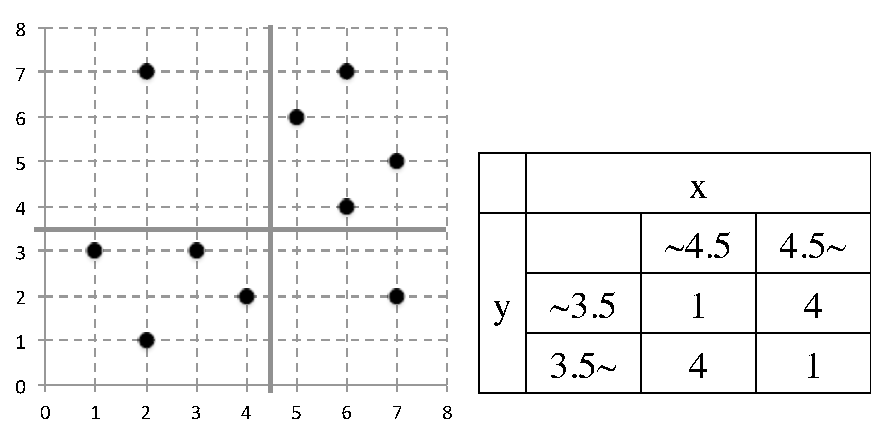
\includegraphics[scale=.50]{figure/mmbucket/split_mbucket.eps}
\end{center}
\caption{One-dimensional partition (mbucket)×2\label{fig:mmbucket_1dim}}
\end{minipage}

\begin{minipage}{0.45\hsize}
\begin{center}
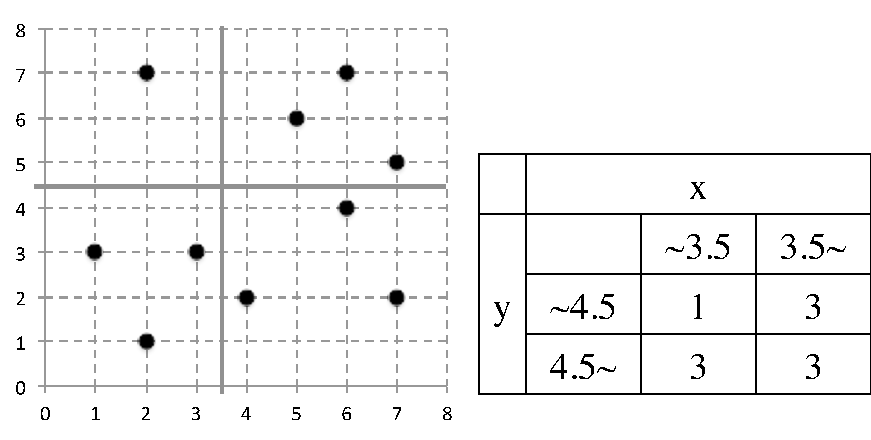
\includegraphics[scale=.50]{figure/mmbucket/split_mmbucket.eps}
\end{center}
\caption{Two-dimensional partition (mmbuket)\label{fig:mmbucket_2dim}}
\end{minipage}

\end{tabular}
\end{center}
\end{figure}


%\begin{figure}[hbt]
%\begin{center}
%\includegraphics[width=20cm,bb=0 0 738 430]{./img/bucket_var.JPG}
%\caption{1次元分割×2による分割と2次元分割による分割の比較}
%\end{center}
%\end{figure}

\subsection*{Precision experiment using on variety of fields}

The following compares the precision of mmbucket and mbucket using real data collected by \href{http://www.pmel.noaa.gov/tao/}{Tropical Atmosphere Ocean (TAO) Project}. The project is designed for the study of year-to-year climate variations related to El Nino the Southern Oscillation (ENSO), and provides provides in-situ data collection of high quality oceanographic and surface meteorological data for monitoring, forecasting, and understanding of climate swings associated with El Nino and La Nina.  Snapshot of the data is shown in the following table. \\



\begin{table}[hbt]
\begin{center}
\caption{Data set used for precision experiment }
{\footnotesize
%\begin{tabular}{p{2em}|p{2.5em}|p{2em}|p{3em}|p{3.5em}|p{4em}|p{4.5em}|p{4.5em}|p{3.5em}|p{3.5em}|p{4.5em}|p{2.5em}}\hline
\begin{tabular}{l|l|l|l|l|l|l|l|l|l|l|l}\hline
%obs  (観測id) & year (年)&month (月)&day (日)&date (日付) &latitude (緯度)&longitude (経度)&zonwinds (東西風速)	&merwinds (南北風速)&humidity (湿度)&air\_temp. (気温)&sstemp (海面温度) \\ \hline
id & year & month & day & date & latitude & longitude & zonwinds & merwinds & humidity & air\_temp. &sstemp \\ \hline
4060 & 93 &5 & 9 & 930509 & -0.02 & -109.96 & -2.1 & 2.1 & 81.2 & 26.8 & 27.02\\
4061 & 93 & 5 & 10 & 930510 & -0.02 & -109.96 & -3.4 & 1.4 & 84.2 & 26.95 & 26.91\\
4062 & 93 & 5 & 11 & 930511 & -0.02 & -109.96 & -3.8 & 2.2 & 84.9 & 26.98 & 26.78\\
4063 & 93 & 5 & 12 & 930512 & -0.02 & -109.96 & -3 & 1.5 & 86.9 & 26.93 & 26.74\\
4064 & 93 & 5 & 13 & 930513 & -0.02 & -109.96 & -4.5 & 1.9 & 87.6 & 27.01 & 26.82\\
4065 & 93 & 5 & 14 & 930514 & -0.02 & -109.96 & -5    & 1.3 & 85.6 & 26.96 & 26.68\\
\hline
\end{tabular}
\\
%latitude:緯度, longitude:経度, zonwinds:東西風速, merwinds:南北風速, humidity:湿度, air\_temp.:気温, sstemp:海面温度
}
\end{center}
\end{table}

The precision experiment uses attributes with numeric values (7 attributes from latitude to sea surface temperature) for bucket partition. The number of record rows is 93,935. Statistics for each attribute is shown in Table 3. "Types of data values" significantly affects computation time of bucket partition.


\begin{table}[hbt]
\begin{center}
\caption{Various statistics of numerical data}
{\footnotesize
\begin{tabular}{c|c|c|c|c|c|c|c} \hline
Measurement & Latitude& Longitude & Zonal wind & North-south wind & Humidity & Temp & Sea surface temp\\ \hline
Type & 482& 924& 228& 206& 385& 1104& 1201\\
Arithmetic average& 0.305& -70.8& -3.35& -0.046& 81.3& 27.1& 27.9\\
Standard deviation & 4.77& 128.7& 3.42& 3.021& 5.28& 1.674& 1.87\\
Minimum & -8.33& -180& -10.7& -10.6& 52.1& 17.5& 18.2\\
Mean & 0.01& -125& -4.1& -0.1& 81.3& 27.5& 28.4\\
Maximum& 9.05& 170.0& 14.3& 13& 99.9& 31.5& 31.0\\ \hline
\end{tabular}
}
\end{center}
\end{table}

The comparison of variance for one-dimensional bucket partition (mbucket) and two-dimensional bucket partition (mmbucket) based on a total of 21 combinations from the 7 attributes are distributed into two columns as shown in Table \ref{tbl:mmbucket_table1}. 

For example, the first row shows the comparison results of bucket partition on “temperature × humidity”, the variance of mbucket is 408274409 and the variance of mmbucket is 406438211, resulting in the ratio of (mmbucket / mbucket) 0.996. The ratio is shown for partitions of 10×10,15×15 and 20×20. The results differs according to the combination of attributes, there are minimal improvements in some combinations such as "humidity × zonal wind speed", improvements can be seen at “latitude x longtitude (15 x 15) with an improvement in accuracy of 19\% (1-0.81).

\begin{table}[hbt]
\begin{center}
\caption{Comparison of two-dimensional partition accuracy of mbucket and mmbucket\label{tbl:mmbucket_table1}}
{\footnotesize
\begin{tabular}{c|c||c|c|c|c|c|c}
\hline
% plastexにてmultirowはNG
%\multirow{2}{*}{項目1} & \multirow{2}{*}{項目2} & \multicolumn{2}{|c|}{分散値(5×5分割)} & \multicolumn{4}{|c}{分散値の比(mmbucket/mbucket)} \\  \cline{3-4}  \cline{5-8}
%                       &  & mbucket  & mmbucket & 5×5 &	10×10 & 15×15 & 20×20  \\ \hline\hline
            &          & \multicolumn{2}{|c|}{Variance (5×5 partition)} & \multicolumn{4}{|c}{Comparison of variance (mmbucket/mbucket)} \\  \cline{3-4}  \cline{5-8}
Item 1       & Item 2    & mbucket  & mmbucket & 5×5  &10×10 &15×15 & 20×20\\ \hline\hline
Temperature        & Humidity     &408274409 &406438211 &0.996 &0.987 &0.988 &0.981 \\
            & Latitude     &374125463 &371258775 &0.992 &0.988 &0.982 &0.964 \\
            & Longitude     &490727955 &454663065 &0.927 &0.949 &0.946 &0.929 \\
            & North-south wind speed &396436813 &394724219 &0.996 &0.991 &0.993 &0.989 \\
            & Sea surface temperature &816199131 &747215787 &0.915 &0.897 &0.883 &0.862 \\
            & Zonal wind speed &382069455 &381225143 &0.998 &0.998 &0.997 &0.996 \\  \hline
Temperature        & Humidity     &368492959 &367941709 &0.999 &0.994 &0.994 &0.990 \\
            & Latitude     &372116309 &370591351 &0.996 &0.991 &0.993 &0.986 \\
            & North-south wind speed &355658757 &355658757 &1.000 &1.000 &1.000 &1.000 \\
            & Sea surface temperature &380382203 &379546293 &0.998 &0.991 &0.991 &0.983 \\
            & Zonal wind speed &357729819 &357697283 &1.000 &1.000 &1.000 &1.000 \\ \hline
Latitude        & Longtitude     &365459223 &361754113 &0.990 &0.923 &0.812 &0.816 \\
            & North-south wind speed &371478669 &370970251 &0.999 &0.988 &0.985 &0.982 \\
            & Sea surface temperature &392810425 &389589403 &0.992 &0.987 &0.979 &0.952 \\
            &  Zonal wind speed &364521077 &364406663 &1.000 &0.999 &0.991 &0.992 \\ \hline
Longtitude        & Latitude &414154185 &408431667 &0.986 &0.976 &0.976 &0.962 \\
            & Sea surface temperature &510979465 &463576537 &0.907 &0.945 &0.939 &0.934 \\
            & Zonal wind speed &400021527 &392710641 &0.982 &0.983 &0.982 &0.973 \\ \hline
North-south wind    & Sea surface temperature &393233841 &392432943 &0.998 &0.995 &0.994 &0.993 \\
            & Zonal wind speed &359290669 &359074015 &0.999 &1.000 &1.000 &0.997 \\ \hline
Sea surface temp    & Zonal wind speed &442877539 &438326669 &0.990 &0.988 &0.984 &0.986 \\ \hline
\end{tabular}
}
\end{center}
\end{table}
 
\subsection*{Speed Comparison}

Next, the experiments are carried out to compare the differences in speed by against different  number of partitions. The execution time is computed using the same data “temperature × sea surface temperature” and “latitude × longitude” with 5 to 40 partitions at increments of 5.  The results are shown in Table \ref{tbl:mmbucket_table2}. The execution time of \verb|mbucket| is consistent regardless of the number of partitions. However, more time is required to compute the number of partitions for two dimensional partitions. This is due to the fact that the algorithm is not efficient in selecting multidimensional orthogonal numeric range required by computation. The partition speed will be noted as possible improvements in the next version. 


\begin{table}[hbt]
\begin{center}
\caption{Sample results of mbucket,mmbucket \label{tbl:mmbucket_table2}}
{\footnotesize
\begin{tabular}{c|c|c|c|c}
\hline
& \multicolumn{2}{|c|}{Temperature×Sea Surface Temperature} & \multicolumn{2}{|c}{Latitude×Longtitude} \\ \hline
Number of buckets &mbucket &mmbucket &mbucket &mmbucket\\ \hline
5 &0.221 &2.21 &0.216 &0.67\\
10 &0.227 &3.90 &0.216 &1.67\\
15 &0.233 &10.4 &0.230 &3.28\\
20 &0.231 &26.1 &0.228 &7.13\\
25 &0.232 &32.9 &0.237 &13.3\\
30 &0.236 &46.7 &0.236 &11.4\\
35 &0.237 &62.3 &0.240 &15.2\\
40 &0.237 &80.1 &0.237 &25.8\\ \hline
\end{tabular}
}
\end{center}
\end{table}

\subsection*{Related Command}
\hyperref[sect:mbucket]{mbucket} : This command processes one-dimensional bucket partition for each field even when more than one field is specified.

%\end{document}




%\documentclass[a4paper]{jsbook}
%\usepackage{mcmd_jp}
%\begin{document}

\section{mminput Display form input screen\label{sect:mminput}}
\index{mminput@mminput}
\underline{Note: This command is a beta. Its specifications may be changed.}

This command displays a data input screen using the text file specified by the \verb|i=| parameter as the screen form. The character strings on the screen form is displayed as is, and the area between square brackets (\verb|[]|) is shown as a freehand input field. There can be two or more input fields. The data entered by the user is output to the CSV file specified by the \verb|o=| parameter. The output data consists of one row. When there are two or more input fields, a multiple-field CSV file is output.
When the command ends with nothing entered in the input frame, null is output. To output a fieldname, use the \verb|f=| parameter. With \verb|f=| omitted, no fieldname header is output. 
The operation is indefinite if the specified coordinate is outside the scope of the terminal.

\subsection*{Format}
\verb/mminput i= [f=] /
\hyperref[sect:option_o]{o=}
\hyperref[sect:option_nfn]{[-nfn]} 
\hyperref[sect:option_nfno]{[-nfno]}  
\hyperref[sect:option_x]{[-x]}
\verb|[--help]|
\verb|[--helpl]|
\verb|[--version]|\\

\subsection*{Parameters}
\begin{table}[htbp]
%\begin{center}
{\small
\begin{tabular}{ll}
\verb|i=| & Specify the text file containing the screen form.\\
\verb|f=| & Specify the output fieldname.\\
\end{tabular} 
}
\end{table} 

\subsection*{Examples}

\subsubsection*{Example 1: Basic example}
A \verb|name| and \verb|address| input screen is displayed. The entered name and address are output to \verb|rsl1.csv| under fieldnames name,address.

\begin{Verbatim}[baselinestretch=0.7,frame=single]
$ more screen.txt

     name   :[               ]
     address:[               ]

$ mminput i=screen.txt f=name,address o=rsl1.csv
$ more rsl1.csv
name,address
Taro,Japan


The following will be displayed:
+--------------------------------------
|
|     name   :[Taro           ]
|     address:[Japan          ]
|
\end{Verbatim}

\subsubsection*{Example 2: Judging end status}
The parameters are the same as in Example 1. This script judges the end status and performs different operations accordingly.

\begin{Verbatim}[baselinestretch=0.7,frame=single]
$ more scp.sh
rm -f rsl3.csv
clear
mminput i=screen.txt f=name,address o=rsl3.csv
if [ $? = 0 ] ; then
  clear ; echo "end by enter key"
else
  clear ; echo "end by escape key"
fi

# Result of typing Taro and Japan and pressing Enter
$ bash scp.sh
end by enter key
$ more rsl3.csv
name,address
Taro,Japan

# Result of typing Taro and Japan and pressing ESC
$ bash scp.sh
end by escape key
$ more rsl3.csv
name,address
Taro,Japan
\end{Verbatim}

\subsection*{Related Commands}
\hyperref[sect:minput] {minput} : Displays the input screen.
\hyperref[sect:mdsp] {mdsp} : Displays a character string at the specified position on the screen.
\hyperref[sect:mseldsp] {mseldsp} : Displays a single-choice input window on the screen.
\hyperref[sect:mmseldsp] {mmseldsp} : Displays a multiple-choice input window on the screen.

%\end{document}


%\documentclass[a4paper]{jsbook}
%\usepackage{mcmd_jp}
%\begin{document}

\section{mmseldsp 複数選択画面入力\label{sect:mmseldsp}}
\index{mmseldsp@mmseldsp}
\underline{注)本コマンドは開発バージョンであり、仕様が変更される可能性があります。}

座標\verb|x=,y=|で指定したターミナル上の位置に\verb|i=|、
もしくは\verb|seldata=|で指定した文字列リストの選択画面を表示し、
ユーザが選んだ文字列を\verb|o=|で指定したファイルに出力する。
\hyperref[sect:mseldsp]{mseldsp}コマンドでは、利用者は一つの選択肢しか選択できないが、
\verb|mmseldsp|は複数の選択肢を選択できる。
選ばれた複数の文字列は、複数行のCSV項目として出力される。
入力枠に何も入力せずに終了した場合は、null値が出力される(すなわち改行だけが出力される)。
\verb|f=|を指定すれば、項目名を出力できる。
\verb|f=|を省略すれば、項目名ヘッダーは出力されない。
選択肢の数が多くて画面をはみ出る場合は、\verb|height=|で
スクロール窓の行数を指定すればよい。

選択画面でエンターキーを押すと、終了ステータス0を返して終了し、
エスケープキーを押すと、終了ステータス1を返して終了する。
いずれのキーで終了しても、選択画面で選ばれた内容はファイルに出力される。

座標は左上が\verb|x=1,y=1|である(エスケープシーケンスの仕様)。
\verb|x=|もしくは\verb|y=|で指定した値が1より小さい場合は、1を指定したものとして動作する。
またターミナルの範囲を超えた座標が指定された場合の動作は不定である。


\subsection*{書式}
\verb/mmseldsp x= y= [f=] [height=] i=|seldata=/
\hyperref[sect:option_o]{o=}
\hyperref[sect:option_nfn]{[-nfn]} 
\hyperref[sect:option_nfno]{[-nfno]}  
\hyperref[sect:option_x]{[-x]}
\hyperref[sect:option_option_tmppath]{[tmpPath=]}
\hyperref[sect:option_precision]{[precision=]}
\verb|[-params]|
\verb|[--help]|
\verb|[--helpl]|
\verb|[--version]|\\

\subsection*{パラメータ}
\begin{table}[htbp]
%\begin{center}
{\small
\begin{tabular}{ll}
\verb|o=|   & 出力ファイル名を指定する。\\
\verb|x=|   & x軸(左から右への横方向)表示開始位置(1以上の値)を指定する。\\
\verb|y=|   & y軸(上から下への縦方向)表示開始位置(1以上の値)を指定する。\\
\verb|height=| & 選択肢を表示する行数。 \\
\verb|i=|   & 選択肢の文字列を項目として持つCSVファイル名 \\
\verb|f=|   & 選択肢の文字列を項目として持つCSVファイル名 \\
\verb|seldata=| & カンマで区切られた選択肢の文字列リスト \\
\end{tabular} 
}
\end{table} 

\subsection*{利用例}

\subsubsection*{例1: 基本例}

ターミナルのx=10,y=2の位置に\verb|sel.txt|の内容を表示し、
利用者が選んだ文字列を\verb|rsl1.txt|に出力する。

\begin{Verbatim}[baselinestretch=0.7,frame=single,commandchars=\\\{\}]
$ more sel.txt
apple
pineapple
grape
orange
$ mmseldsp x=10 y=2 i=sel.txt o=rsl1.txt
# 利用者が一行目を選んだとする。
$ mose rsl1.txt
apple
orange


以下、画面イメージ
+--------------------------------------
|
|          \textColor{red}{black}{apple    }
|          \textColor{white}{black}{pineapple}
|          \textColor{white}{black}{grape}
|          \textColor{red}{black}{orange   }
|
\end{Verbatim}

\subsubsection*{例2: 引数で与える例}

例1と同様で、選択肢の文字列を\verb|seldata=|で与える。

\begin{Verbatim}[baselinestretch=0.7,frame=single,commandchars=\\\{\}]
$ mmseldsp x=10 y=2 seldata=apple,pineapple,grape,orange o=rsl2.txt
# 利用者が二行目を選んだとする。
$ mose rsl2.txt
apple
grape


以下、画面イメージ
+--------------------------------------
|
|
|          \textColor{red}{black}{apple    }
|          \textColor{white}{black}{pineapple}
|          \textColor{red}{black}{grape    }
|          \textColor{white}{black}{orange}
|
\end{Verbatim}

\subsubsection*{例3: 終了ステータスを判定する例}

例2と同じパラメータで実行し、終了ステータスを判定して異なる動作をするスクリプトの例。

\begin{Verbatim}[baselinestretch=0.7,frame=single]
$ more scp.sh
rm -f rsl3.csv
clear
mmseldsp x=10 y=2 seldata=apple,pineapple,grape,orange o=rsl3.csv
if [ $? = 0 ] ; then
  clear ; echo "end by enter key"
else
  clear ; echo "end by escape key"
fi

# appleを選択後enterキーを入力した場合の結果
$ bash scp.sh
end by enter key
$ more rsl3.csv
apple

# appleを選択後escapeキーを入力した場合の結果
$ bash scp.sh
end by escape key
$ more rsl3.csv
apple
\end{Verbatim}

\subsection*{関連コマンド}
\hyperref[sect:minput] {minput} :入力画面を表示する。

\hyperref[sect:mminput] {mminput} : 複数入力枠による入力画面を表示する。

\hyperref[sect:mdsp] {mdsp} : 画面の指定位置に文字列を表示する。

\hyperref[sect:mseldsp] {mseldsp} : 画面に単一選択入力窓を表示する。


%\end{document}


%\begin{document}

\section{mmvavg - Calculate Moving Average\label{sect:mmvavg}}
\index{mmvavg@mmvavg}

Calculate the moving average. The three different ways to calculate moving average include simple moving average ($SMA$), weighted moving average ($WMA$), and exponential moving average ($EMA$). 


\if0 #no help# following sentences will not apear on the help document. \fi

The value of $t$ time is expressed by $x_t$, and period is represented by $m$ as defined in several formulas of moving average (\ref{eq:sma},\ref{eq:wma},\ref{eq:ema}).


\begin{eqnarray}
%\begin{footnotesize}
SMA_t=\frac{1}{m} \sum_{i=0}^{m-1} x_{t-i}
\label{eq:sma}
%\end{footnotesize}
\end{eqnarray}

\begin{eqnarray}
%\begin{footnotesize}
WMA_t=\sum_{i=0}^{m-1} \frac{m-i}{S} x_{t-i},\ \ S=\sum_{i=1}^m i
\label{eq:wma}
%\end{footnotesize}
\end{eqnarray}

\begin{eqnarray}
%\begin{footnotesize}
EMA_t=\alpha x_t + (1-\alpha)EMA_{t-1}
\label{eq:ema}
%\end{footnotesize}
\end{eqnarray}

\subsection*{Format}
\verb/mmvavg [s=] [k=] [n=] f= [t=] [-exp|-w] [alpha=] [skip=]/
\hyperref[sect:option_i]{[i=]}
\hyperref[sect:option_o]{[o=]}
\hyperref[sect:option_assert_diffSize]{[-assert\_diffSize]}
\hyperref[sect:option_assert_nullkey]{[-assert\_nullkey]}
\hyperref[sect:option_assert_nullin]{[-assert\_nullin]}
\hyperref[sect:option_assert_nullout]{[-assert\_nullout]}
\hyperref[sect:option_nfn]{[-nfn]} 
\hyperref[sect:option_nfno]{[-nfno]}  
\hyperref[sect:option_x]{[-x]}
\hyperref[sect:option_q]{[-q]}
\hyperref[sect:option_option_tmppath]{[tmpPath=]}
\hyperref[sect:option_precision]{[precision=]}
\verb|[--help]|
\verb|[--helpl]|
\verb|[--version]|\\

\subsection*{Parameters}
\begin{table}[htbp]
%\begin{center}
{\small
\begin{tabular}{ll}
\verb|s=|    & After the specified field is sorted (multiple fields can be specified), moving average is calculated. \\
             & \verb|s=| parameter is required when \verb|-q| option is not specified. \\
\verb|k=|    & Aggregate records using the specified field name(s) (multiple fields can as unit of calculation. \\
\verb|f=|    & Compute the moving averages of the field(s) (multiple fields can be specified). \\
\verb|t=|    & Interval numbers of integers greater than 1.  \\
             & When \verb|-exp| is used with \verb|alpha=|, the \verb|t=| parameter do not need to be defined. \\
\verb|-w|    & Linear weighted moving average.\\
\verb|-exp|  & Exponential smoothing moving average. \\
\verb|alpha=|& Use a real number as smoothing coefficient when \verb|-exp| is specified. \\
             & The default value of alpha is \verb|alpha=2/(value of = t+1)|。\\
\verb|skip=| & Specify the number of rows to hide from the top in the output. \\
             & Default value: \verb|skip=(value of t= -1)|, \verb|skip=0| when \verb|-exp| is specified.  \\
\end{tabular} 
}
\end{table} 


\subsection*{Examples}
\subsubsection*{Example 1: Basic Example}

The first row is not printed as there is less than the number of required intervals for computation.


\begin{Verbatim}[baselinestretch=0.7,frame=single]
$ more dat1.csv
id,value
1,5
2,1
3,3
4,4
5,4
6,6
7,1
8,4
9,7
$ mmvavg s=id f=value t=2 i=dat1.csv o=rsl1.csv
#END# kgmvavg f=value i=dat1.csv o=rsl1.csv s=id t=2
$ more rsl1.csv
id%0,value
2,3
3,2
4,3.5
5,4
6,5
7,3.5
8,2.5
9,5.5
\end{Verbatim}
\subsubsection*{Example 2: Basic Example 2}

The first row is not printed as there is less than the number of required intervals for computation.


\begin{Verbatim}[baselinestretch=0.7,frame=single]
$ mmvavg s=id f=value t=2 -w i=dat1.csv o=rsl2.csv
#END# kgmvavg -w f=value i=dat1.csv o=rsl2.csv s=id t=2
$ more rsl2.csv
id%0,value
2,2.333333333
3,2.333333333
4,3.666666667
5,4
6,5.333333333
7,2.666666667
8,3
9,6
\end{Verbatim}
\subsubsection*{Example 3: Basic Example 3}

Exponential smoothing moving average (\verb|-exp|) includes the first row in the output.


\begin{Verbatim}[baselinestretch=0.7,frame=single]
$ mmvavg s=id f=value t=2 -exp i=dat1.csv o=rsl3.csv
#END# kgmvavg -exp f=value i=dat1.csv o=rsl3.csv s=id t=2
$ more rsl3.csv
id%0,value
1,5
2,2.333333333
3,2.777777778
4,3.592592593
5,3.864197531
6,5.288065844
7,2.429355281
8,3.47645176
9,5.82548392
\end{Verbatim}
\subsubsection*{Example 4: An example of assigning key}



\begin{Verbatim}[baselinestretch=0.7,frame=single]
$ more dat2.csv
id,key,value
1,a,5
2,a,1
3,a,3
4,a,4
5,a,4
6,b,6
7,b,1
8,b,4
9,b,7
$ mmvavg s=key,id k=key f=value t=2 i=dat2.csv o=rsl4.csv
#END# kgmvavg f=value i=dat2.csv k=key o=rsl4.csv s=key,id t=2
$ more rsl4.csv
id,key,value
2,a,3
3,a,2
4,a,3.5
5,a,4
7,b,3.5
8,b,2.5
9,b,5.5
\end{Verbatim}
\subsubsection*{Example 5: Display all records including those that are less than the defined intervals }



\begin{Verbatim}[baselinestretch=0.7,frame=single]
$ more dat3.csv
key,value
a,1
a,2
a,3
a,4
a,5
b,6
b,1
b,4
b,7
$ mmvavg -q k=key f=value t=2 skip=0 i=dat3.csv o=rsl5.csv
#END# kgmvavg -q f=value i=dat3.csv k=key o=rsl5.csv skip=0 t=2
$ more rsl5.csv
key,value
a,1
a,1.5
a,2.5
a,3.5
a,4.5
b,6
b,3.5
b,2.5
b,5.5
\end{Verbatim}

\subsection*{Related Commands}
\hyperref[sect:mmvstats] {mmvstats} : Specify the average as well as various types of statistics. 

\hyperref[sect:mmvsim] {mmvsim} : Compute bivariate statistics. 

\hyperref[sect:mwindow] {mwindow} : Computes statistics on sliding window data which cannot be computed using \verb|mmvstats|. 

%\end{document}


%\documentclass[a4paper]{jsbook}
%\usepackage{mcmd_jp}
%\begin{document}

\section{mmvsim 移動窓の類似度計算\label{sect:mmvsim}}
\index{mmvsim@mmvsim}

移動窓を設定し、各種類似度(2変量の統計量)を計算する。
\hyperref[sect:msim]{msim}コマンドの移動窓バージョンとして考えればよい。
\verb|msim|との違いは、指定できる類似度は一つだけで、また類似度計算の対象項目は2つのみである。

\subsection*{書式}
\verb|mmvsim [s=] [k=] f= c= a= [t=] [skip=] [-n] |
\hyperref[sect:option_i]{[i=]}
\hyperref[sect:option_o]{[o=]}
\hyperref[sect:option_assert_diffSize]{[-assert\_diffSize]}
\hyperref[sect:option_assert_nullkey]{[-assert\_nullkey]}
\hyperref[sect:option_assert_nullin]{[-assert\_nullin]}
\hyperref[sect:option_assert_nullout]{[-assert\_nullout]}
\hyperref[sect:option_nfn]{[-nfn]} 
\hyperref[sect:option_nfno]{[-nfno]}  
\hyperref[sect:option_x]{[-x]}
\hyperref[sect:option_q]{[-q]}
\hyperref[sect:option_option_tmppath]{[tmpPath=]}
\hyperref[sect:option_precision]{[precision=]}
\verb|[-params]|
\verb|[--help]|
\verb|[--helpl]|
\verb|[--version]|\\

\subsection*{パラメータ}
\begin{table}[htbp]
%\begin{center}
{\small
\begin{tabular}{ll}
\verb|i=|    & 入力ファイル名を指定する。\\
\verb|o=|    & 出力ファイル名を指定する。\\
\verb|s=|    & ここで指定した項目(複数項目指定可)で並べ替えられた後、各種類似度が計算される。\\
             & \verb|-q|オプションを指定しないとき、\verb|s=|パラメータは必須。\\
\verb|k=|    & ここで指定された項目(複数項目指定可)を単位として集計する。 \\
\verb|f=|    & 集計項目名リスト(複数項目指定可)を指定する。\\
\verb|t=|    & 期間数を1以上の整数で指定する。 \\
\verb|c=|    & 類似度(以下のリストから一つだけ)指定する。\\
             & \verb/covar|ucovar|pearson|spearman|kendall|euclid|/\\
             & \verb/cosine|cityblock|hamming|chi|phi|jaccard|support|lift/ \\
             & 詳細な定義は\hyperref[sect:msim]{msim}コマンドを参照のこと。\\
\verb|skip=| & 出力を抑制する最初の行数を指定する。【デフォルト値:\verb|skip=(t=の値-1)|】\\
\verb|a=| & 計算結果の出力として追加される項目の名前を指定する。 \\
\verb|-n| & 期間内にNULL値が1つでも含まれていると結果もNULL値とする。\\
\end{tabular} 
}
\end{table} 

\subsection*{利用例}
\subsubsection*{Example 1: Basic Example}

Calculate the Pearson product-moment correlation coefficient for 3 window intervals for fields \verb|x,y|.


\begin{Verbatim}[baselinestretch=0.7,frame=single]
$ more dat1.csv
t,x,y
1,14,0.17
2,11,0.2
3,32,0.15
4,13,0.33
5,8,0.1
6,19,0.56
$ mmvsim s=t t=3 c=pearson f=x,y a=sim i=dat1.csv o=rsl1.csv
#END# kgmvsim a=sim c=pearson f=x,y i=dat1.csv o=rsl1.csv s=t t=3
$ more rsl1.csv
t%0,x,y,sim
3,32,0.15,-0.8746392857
4,13,0.33,-0.6515529194
5,8,0.1,-0.1164257338
6,19,0.56,0.9986254289
\end{Verbatim}


\subsection*{関連コマンド}
\hyperref[sect:msim] {msim} : 移動窓を設定せずに類似度計算を行う。

\hyperref[sect:mwindow] {mwindow} : 動窓のデータを作成するので、そのデータを使えば\verb|mmvstats|で計算できない統計量も計算可能。

\hyperref[sect:mmvavg] {mmvavg} : 移動平均に限定した計算を行う。

%\end{document}


%\documentclass[a4paper]{jsbook}
%\usepackage{mcmd_jp}
%\begin{document}

\section{mmvstats 移動窓の統計量の計算\label{sect:mmvstats}}
\index{mmvstats@mmvstats}

移動窓を設定し、各種統計量(1変量)を計算する。
\hyperref[sect:mstats]{mstats}コマンドの移動窓バージョンとして考えればよい。

\subsection*{書式}
\verb|mmvstats [s=] [k=] f= [t=] c= [skip=] -n |
\hyperref[sect:option_i]{[i=]}
\hyperref[sect:option_o]{[o=]}
\hyperref[sect:option_assert_diffSize]{[-assert\_diffSize]}
\hyperref[sect:option_assert_nullkey]{[-assert\_nullkey]}
\hyperref[sect:option_assert_nullin]{[-assert\_nullin]}
\hyperref[sect:option_assert_nullout]{[-assert\_nullout]}
\hyperref[sect:option_nfn]{[-nfn]} 
\hyperref[sect:option_nfno]{[-nfno]}  
\hyperref[sect:option_x]{[-x]}
\hyperref[sect:option_q]{[-q]}
\hyperref[sect:option_option_tmppath]{[tmpPath=]}
\hyperref[sect:option_precision]{[precision=]}
\verb|[-params]|
\verb|[--help]|
\verb|[--helpl]|
\verb|[--version]|\\

\subsection*{パラメータ}
\begin{table}[htbp]
%\begin{center}
{\small
\begin{tabular}{ll}
\verb|i=|    & 入力ファイル名を指定する。\\
\verb|o=|    & 出力ファイル名を指定する。\\
\verb|s=|    & ここで指定した項目(複数項目指定可)で並べ替えられた後、各種統計量が計算される。\\
             & \verb|-q|オプションを指定しないとき、\verb|s=|パラメータは必須。\\
\verb|k=|    & ここで指定された項目(複数項目指定可)を単位として集計する。\\
\verb|f=|    & 集計項目名リスト(複数項目指定可)を指定する。\\
\verb|t=|    & 期間数を1以上の整数で指定する。 \\
\verb|c=|    & 統計量(以下のリストから一つだけ指定可)\\
             & \verb/sum|mean|devsq|var|uvar|sd|usd|cv|min|/\\
             & \verb/|max|range|skew|uskew|kurt|ukurt/\\
             & 詳細な定義は\hyperref[sect:mstats]{mstats}コマンドを参照のこと。\\
\verb|skip=| & 出力を抑制する最初の行数\\
\verb|-n| & 期間内にNULL値が1つでも含まれていると結果もNULL値とする。\\
\end{tabular} 
}
\end{table} 


\subsection*{利用例}
\subsubsection*{例1: 基本例}

移動窓の合計を計算する。
最初の行は期数に満たないため出力されない。


\begin{Verbatim}[baselinestretch=0.7,frame=single]
$ more dat1.csv
id,value
1,5
2,1
3,3
4,4
5,4
6,6
7,1
8,4
9,7
$ mmvstats s=id f=value t=2 c=sum i=dat1.csv o=rsl1.csv
#END# kgmvstats c=sum f=value i=dat1.csv o=rsl1.csv s=id t=2
$ more rsl1.csv
id%0,value
2,6
3,4
4,7
5,8
6,10
7,7
8,5
9,11
\end{Verbatim}

\subsection*{関連コマンド}
\hyperref[sect:mmvavg] {mmvavg} : 移動平均に限定した計算を行う。

\hyperref[sect:mwindow] {mwindow} : 動窓のデータを作成するので、そのデータを使えば\verb|mmvstats|で計算できない統計量も計算可能。

\hyperref[sect:mmvsim] {mmvsim} : 移動窓の類似度(2変量統計量)の計算を行う。

%\end{document}


%\begin{document}

\section{mnewnumber - Generate List of Sequential Numbers\label{sect:mnewnumber}}
\index{mnewnumber@mnewnumber}
Define the start value of the alphabetic sequence at the \verb|S=| parameter, set the the interval of alphabet sequence at \verb|I=| parameter, and define the column name of the sequence at \verb|a=| parameter. 
The alphabet sequence uses 26 alphabetic characters in base-26 from A to Z (A,B,$\cdots$,Z,AA,AB,$\cdots$,AZ,BA,BB,$\cdots$,ZZ,AAA,AAB,$\cdots$).



\subsection*{Format}
\verb|mnewnumber a= [I=] [S=] [l=]|
\hyperref[sect:option_o]{[o=]}
\hyperref[sect:option_nfn]{[-nfn]} 
\hyperref[sect:option_nfno]{[-nfno]}  
\hyperref[sect:option_x]{[-x]}
\hyperref[sect:option_q]{[-q]}
\hyperref[sect:option_option_tmppath]{[tmpPath=]}
\verb|[--help]|
\verb|[--helpl]|
\verb|[--version]|\\

\subsection*{Parameters}
\begin{table}[htbp]
%\begin{center}
{\small
\begin{tabular}{ll}
\verb|a=|    & Specify the field name of the list of new serials.\\
             & This parameter is not required when \verb|-nfn,-nfno| option is specified. \\
\verb|I=|    & Interval between the sequence of numbers [default value: 1]\\
\verb|S=|    & Starting value/alphabet(upper case letters) [default value:1]\\
             & Assign either alphabet or numbers as the starting value of the sequence.\\
             & A list of serial numbers is generated when the starting numeric value is specified. \\
             & An alphabet sequence is generated when the starting alphabet is specified (cannot be specified in lowercase). \\
\verb|l=|    & Number of rows to generate [default value:10]\\
\end{tabular} 
}
\end{table} 


\subsection*{Examples}
\subsubsection*{Example 1: Basic Example}

Generate a dataset with 5 sequential numbers starting from 1 incremented by 1. Name the sequence as \verb|No.|.


\begin{Verbatim}[baselinestretch=0.7,frame=single]
$ mnewnumber a=No. I=1 S=1 l=5 o=rsl1.csv
#END# kgNewnumber I=1 S=1 a=No. l=5 o=rsl1.csv
$ more rsl1.csv
No.
1
2
3
4
5
\end{Verbatim}
\subsubsection*{Example 2: Change the starting number and interval }

Generate a dataset consisting of 5 sequential numbers starting from 10 with an incremental interval of 5. Name the sequence as \verb|No.|.


\begin{Verbatim}[baselinestretch=0.7,frame=single]
$ mnewnumber a=No. I=5 S=10 l=5 o=rsl2.csv
#END# kgNewnumber I=5 S=10 a=No. l=5 o=rsl2.csv
$ more rsl2.csv
No.
10
15
20
25
30
\end{Verbatim}
\subsubsection*{Example 3: Generate series of alphabet}

Generate a dataset consisting of 5 alphabet sequence starting from A with 1 alphabet in between. Name the sequence as \verb|No.|.


\begin{Verbatim}[baselinestretch=0.7,frame=single]
$ mnewnumber a=No. I=1 S=A l=5 o=rsl3.csv
#END# kgNewnumber I=1 S=A a=No. l=5 o=rsl3.csv
$ more rsl3.csv
No.
A
B
C
D
E
\end{Verbatim}
\subsubsection*{Example 4: Generate data without header}

Generate a dataset consisting of 11 alphabet sequence starting from B with 3 alphabets in between. Exclude the header from the output.


\begin{Verbatim}[baselinestretch=0.7,frame=single]
$ mnewnumber  -nfn  I=3 l=11 S=B o=rsl4.csv
#END# kgNewnumber -nfn I=3 S=B l=11 o=rsl4.csv
$ more rsl4.csv
B
E
H
K
N
Q
T
W
Z
AC
AF
\end{Verbatim}


\subsection*{Related Commands}
\hyperref[sect:mnewrand] {mnewrand} : Generate a dataset with random numbers. 

\hyperref[sect:mnewstr] {mnewstr} : Generate fixed character strings. 

%\end{document}


%\begin{document}

\section{mnewrand 乱数データの新規生成\label{sect:mnewrand}}
\index{mnewrand@mnewrand}
0.0から1.0の範囲の実数乱数を生成する。
\verb|-int|を指定することで、整数乱数を生成することもできる。

乱数の生成にはメルセンヌ・ツイスター法を利用している
(\href{http://www.math.sci.hiroshima-u.ac.jp/~m-mat/MT/emt.html}{原作者のページ}
, \href{http://www.boost.org/doc/libs/1_54_0/doc/html/boost_random.html}{boostライブラリ})。


\subsection*{書式}
\verb|mnewrand a= [max=] [min=] [S=] [l=] [-int]|
\hyperref[sect:option_o]{[o=]}
\hyperref[sect:option_nfn]{[-nfn]} 
\hyperref[sect:option_nfno]{[-nfno]}  
\hyperref[sect:option_x]{[-x]}
\hyperref[sect:option_option_tmppath]{[tmpPath=]}
\hyperref[sect:option_precision]{[precision=]}
\verb|[-params]|
\verb|[--help]|
\verb|[--helpl]|
\verb|[--version]|\\

\subsection*{パラメータ}
\begin{table}[htbp]
%\begin{center}
{\small
\begin{tabular}{ll}
\verb|o=|      & 出力ファイル名を指定する。\\
\verb|a=|      & 新規に作成するデータの項目名を指定する。\\
               & \verb|-nfn,-nfno|オプション指定時は指定の必要はない。\\
\verb|max=|    & 乱数の最大値を指定する。【デフォルト値:INT\_MAX】\\
               & このパラメータを指定するときは\verb|-int|も指定しなければならない。\\
\verb|min=|    & 乱数の最小値を指定する。【デフォルト値:0】\\
               & このパラメータを指定するときは\verb|-int|も指定しなければならない。\\
\verb|S=|      & 乱数の種を指定する。【デフォルト値:現在時刻】\\
\verb|l=|      & 行数【デフォルト値:10】\\
               & 新規作成する乱数データの行数を指定する。\\
\verb|-int|    & 整数乱数を生成する\\
\end{tabular} 
}
\end{table} 


\subsection*{利用例}
\subsubsection*{Example 1: Basic Example}

Generate 10 rows of random integers. Use a fixed random seed so that it will always return the same sequence of random numbers.


\begin{Verbatim}[baselinestretch=0.7,frame=single]
$ mnewrand a=rand S=1 o=rsl1.csv
#END# kgnewrand S=1 a=rand o=rsl1.csv
$ more rsl1.csv
rand
0.4170219984
0.9971848081
0.7203244893
0.9325573612
0.0001143810805
0.1281244478
0.3023325677
0.9990405154
0.1467558926
0.2360889763
\end{Verbatim}
\subsubsection*{Example 2: Random Integers}

Use random seed 1 to generate 5 rows of random integers with minimum value of 10 and maximum value of 100.


\begin{Verbatim}[baselinestretch=0.7,frame=single]
$ mnewrand a=rand -int max=1000 min=0 l=5 S=1 o=rsl2.csv
#END# kgnewrand -int S=1 a=rand l=5 max=1000 min=0 o=rsl2.csv
$ more rsl2.csv
rand
417
998
721
933
0
\end{Verbatim}
\subsubsection*{Example 3: Generate Output without Header}

Specify \verb|-nfn| option to generate random number data without header.


\begin{Verbatim}[baselinestretch=0.7,frame=single]
$ mnewrand -nfn l=5 S=1 o=rsl3.csv
#END# kgnewrand -nfn S=1 l=5 o=rsl3.csv
$ more rsl3.csv
0.4170219984
0.9971848081
0.7203244893
0.9325573612
0.0001143810805
\end{Verbatim}


\subsection*{関連コマンド}
\hyperref[sect:mnewnumber] {mnewnumber} : 連番を生成する。

\hyperref[sect:mnewstr] {mnewstr} : 固定文字列を生成する。

%\end{document}


%\begin{document}

\section{mnewstr - Generate Fixed String Data\label{sect:mnewstr}}
\index{mnewstr@mnewstr}
Define the character string to generate at \verb|v=| parameter, and pass the new column name at \verb|a=| parameter. Multiple columns can be generated at a time. 


\subsection*{Format}
\verb|mnewstr a= [v=] [l=]|
\hyperref[sect:option_o]{[o=]}
\hyperref[sect:option_nfn]{[-nfn]} 
\hyperref[sect:option_nfno]{[-nfno]}  
\hyperref[sect:option_x]{[-x]}
\hyperref[sect:option_q]{[-q]}
\hyperref[sect:option_option_tmppath]{[tmpPath=]}
\verb|[--help]|
\verb|[--helpl]|
\verb|[--version]|\\

\subsection*{Parameters}
\begin{table}[htbp]
%\begin{center}
{\small
\begin{tabular}{ll}
\verb|a=|    & Field name(s) of the new data. \\
             & Define multiple field names separated with a comma in between the field names. \\
             & This argument is not required when  \verb|-nfn,-nfno| options are specified.\\
\verb|v=|    & Specify the new character string to generate. \\
             & Define multiple field separated with a comma in between the values. \\
             & The number of fields must be the same as the number of field names defined at \verb|a=|.  \\
\verb|l=|    & Number of rows of random data to generate [default value:10]. \\

\end{tabular} 
}
\end{table} 


\subsection*{Examples}
\subsubsection*{Example 1: Basic Example}

Generate a new dataset with characters strings \verb|custNo| and \verb|A0001| printed in 5 rows, and name the fields as \verb|attribute| and \verb|code| respectively.


\begin{Verbatim}[baselinestretch=0.7,frame=single]
$ mnewstr a=attribute,code v=custNo,A0001 l=5 o=rsl1.csv
#END# kgnewstr a=attribute,code l=5 o=rsl1.csv v=custNo,A0001
$ more rsl1.csv
attribute,code
custNo,A0001
custNo,A0001
custNo,A0001
custNo,A0001
custNo,A0001
\end{Verbatim}

\subsection*{Related Commands}
\hyperref[sect:mnewnumber] {mnewnumber} : Generate list of sequential numbers in a new dataset. 

\hyperref[sect:mnewrand] {mnewrand} : Generate random numbers in a new dataset. 

%\end{document}


%\begin{document}

\section{mnjoin - Natural Join with Reference File\label{sect:mnjoin}}
\index{mnjoin@mnjoin}

A natural join selects rows from input data and reference file that have equal values in columns defined at \verb|k=| parameter, the reference file is specified at the \verb|m=| parameter, fields in the reference file specified at \verb|f=| parameter is added through natural join. The difference with \verb|mjoin| command is that key field(s) in the reference field is not unique.  

Given that the input data has $n$ records with a certain key value, and the reference file has $m$ records with the same key value, $n\times m$ records will be generated. In addition, if \verb|f=| is not defined, all fields except the key field will be added. 


\subsection*{Format}
\verb/mnjoin k= [f=] [K=] [-n] [-N] m=|/ 
\hyperref[sect:option_i]{i=}
\hyperref[sect:option_o]{[o=]}
\hyperref[sect:option_bufcount]{[bufcount=]} 
\hyperref[sect:option_nfn]{[-nfn]} 
\hyperref[sect:option_nfno]{[-nfno]}  
\hyperref[sect:option_assert_diffSize]{[-assert\_diffSize]}
\hyperref[sect:option_assert_nullkey]{[-assert\_nullkey]}
\hyperref[sect:option_assert_nullin]{[-assert\_nullin]}
\hyperref[sect:option_assert_nullout]{[-assert\_nullout]}
\hyperref[sect:option_x]{[-x]}
\hyperref[sect:option_q]{[-q]}
\hyperref[sect:option_option_tmppath]{[tmpPath=]}
\verb|[--help]|
\verb|[--helpl]|
\verb|[--version]|\\

\subsection*{Parameters}
\begin{table}[htbp]
%\begin{center}
{\small
\begin{tabular}{ll}
\verb|k=|    & key field name(s) from the input data for matching \\
             & This key field is specified in the input data and at the \verb|K=| parameter.  \\
             & Join rows when this fields matches with the fields from the reference data. \\
\verb|f=|    & Specify the field name(s) to join from the reference file. \\
             & When this parameter is not defined, all fields except the key field will be joined. \\
\verb|m=|    & Reference file name. \\
             & Read from standard input if this parameter is not set. (when \verb|i=| is specified) \\
\verb|K=|    & Key field name(s) from the reference data for matching \\
             & This key field(s) from reference data is compared with the key field(s) from  input data specified at \verb|k=| parameter, \\
             & fields where records with common key are joined. \\
             & This parameter is not required if the field name in reference file is the same as the one defined at the \verb|k=|parameter. \\
\verb|-n|    & Output NULL values when reference data does not consist of input data. \\
\verb|-N|    & Output NULL values when input data does not consist of reference data. \\
\end{tabular} 
}
\end{table} 

\subsection*{Examples}
\subsubsection*{Example 1: Basic Example }

The \verb|item| field in the input file is compared with the \verb|item| field from the reference file, add \verb|cost| field for records with the same value. There are two records where \verb|item=A| in both input file and reference file, therefore, 2$\times$2=4 rows of \verb|item=A| is written to the output file.


\begin{Verbatim}[baselinestretch=0.7,frame=single]
$ more dat1.csv
item,date,price
A,20081201,100
A,20081213,98
B,20081002,400
B,20081209,450
C,20081201,100
$ more ref1.csv
item,cost
A,50
A,70
B,300
E,200
$ mnjoin k=item f=cost m=ref1.csv i=dat1.csv o=rsl1.csv
#END# kgnjoin f=cost i=dat1.csv k=item m=ref1.csv o=rsl1.csv
$ more rsl1.csv
item%0,date,price,cost
A,20081201,100,50
A,20081201,100,70
A,20081213,98,50
A,20081213,98,70
B,20081002,400,300
B,20081209,450,300
\end{Verbatim}
\subsubsection*{Example 2: Ouput unmatched data}

Use \verb|-n| to print records in the input data that do not match with those in the reference file (row where \verb|item="C"|), and use -N to print records in the reference file that do not match with those in the input file (row where \verb|item="E"|).


\begin{Verbatim}[baselinestretch=0.7,frame=single]
$ more ref2.csv
item,cost
A,50
B,300
E,200
$ mnjoin k=item f=cost m=ref2.csv -n -N i=dat1.csv o=rsl2.csv
#END# kgnjoin -N -n f=cost i=dat1.csv k=item m=ref2.csv o=rsl2.csv
$ more rsl2.csv
item%0,date,price,cost
A,20081201,100,50
A,20081213,98,50
B,20081002,400,300
B,20081209,450,300
C,20081201,100,
E,,,200
\end{Verbatim}

\subsection*{Related Commands}
\hyperref[sect:mjoin] {mjoin} :  It is faster to use \verb|mjoin| if the key in the reference file is unique. 

\hyperref[sect:mproduct] {mproduct} : Join combination of all records without using key. Each row in the reference file is joined with all records in the input data.

%\end{document}


%\begin{document}

\section{mnormalize - Normalization\label{sect:mnormalize}}
\index{mnormalize@mnormalize}

Specify the field at the \verb|f=| parameter, and specify the normalization method at \verb|c=| parameter.\\

\subsection*{Format}
\verb|mnormalize c= f= [k=]| 
\hyperref[sect:option_i]{[i=]}
\hyperref[sect:option_o]{[o=]}
\hyperref[sect:option_bufcount]{[bufcount=]} 
\hyperref[sect:option_assert_diffSize]{[-assert\_diffSize]}
\hyperref[sect:option_assert_nullkey]{[-assert\_nullkey]}
\hyperref[sect:option_assert_nullin]{[-assert\_nullin]}
\hyperref[sect:option_assert_nullout]{[-assert\_nullout]}
\hyperref[sect:option_nfn]{[-nfn]} 
\hyperref[sect:option_nfno]{[-nfno]}  
\hyperref[sect:option_x]{[-x]}
\hyperref[sect:option_q]{[-q]}
\hyperref[sect:option_option_tmppath]{[tmpPath=]}
\hyperref[sect:option_precision]{[precision=]}
\verb|[--help]|
\verb|[--helpl]|
\verb|[--version]|\\

\subsection*{Parameters}
\begin{table}[htbp]
%\begin{center}
{\small
\begin{tabular}{ll}
\verb|c=|    & Specify the normalisation method listed as follows.\\
             & \verb|z| : z score : $z_i=(x_i-m)/u$ ($x_i$: $i$number of data, $m$ :arithmetic mean, $u$ :standard deviation)\\
             & \verb|Z| : deviation value : $Z_i=50+10\times z_i$\\
             & \verb|range| : use linear conversion to transform minimum value 0 to maximum value 1 $r_i=(x_i-\min_x)/(\max_x-\min_x)$\\
\verb|f=|    & Specify the field to normalize here. \\
             & Specify the new field name after :(colon). Example: \verb|f=|quantity:quantityNorm\\
\verb|k=|    & Key field name(s) [\hyperref[sect:option_k]{aggregate key break processing}]\\
             & The key field specified is used as the unit for normalization. \\
\end{tabular} 
}
\end{table} 

\subsection*{Examples}
\subsubsection*{例1: 基本例}

「顧客」を単位にして「数量」と「金額」項目を基準化(z得点)し、
「数量基準値」と「金額基準値」という項目名で出力する。


\begin{Verbatim}[baselinestretch=0.7,frame=single]
$ more dat1.csv
顧客,数量,金額
A,1,10
A,2,20
B,1,15
B,3,10
B,1,20
$ mnormalize c=z k=顧客 f=数量:数量基準値,金額:金額基準値 i=dat1.csv o=rsl1.csv
#END# kgnormalize c=z f=数量:数量基準値,金額:金額基準値 i=dat1.csv k=顧客 o=rsl1.csv
$ more rsl1.csv
顧客%0,数量,金額,数量基準値,金額基準値
A,1,10,-0.7071067812,-0.7071067812
A,2,20,0.7071067812,0.7071067812
B,1,15,-0.5773502692,0
B,3,10,1.154700538,-1
B,1,20,-0.5773502692,1
\end{Verbatim}
\subsubsection*{例2: 偏差値}



\begin{Verbatim}[baselinestretch=0.7,frame=single]
$ mnormalize c=Z k=顧客 f=数量:数量基準値,金額:金額基準値 i=dat1.csv o=rsl2.csv
#END# kgnormalize c=Z f=数量:数量基準値,金額:金額基準値 i=dat1.csv k=顧客 o=rsl2.csv
$ more rsl2.csv
顧客%0,数量,金額,数量基準値,金額基準値
A,1,10,42.92893219,42.92893219
A,2,20,57.07106781,57.07106781
B,1,15,44.22649731,50
B,3,10,61.54700538,40
B,1,20,44.22649731,60
\end{Verbatim}
\subsubsection*{例3: 0から1への線形変換}



\begin{Verbatim}[baselinestretch=0.7,frame=single]
$ mnormalize c=range k=顧客 f=数量:数量基準値,金額:金額基準値 i=dat1.csv o=rsl3.csv
#END# kgnormalize c=range f=数量:数量基準値,金額:金額基準値 i=dat1.csv k=顧客 o=rsl3.csv
$ more rsl3.csv
顧客%0,数量,金額,数量基準値,金額基準値
A,1,10,0,0
A,2,20,1,1
B,1,15,0,0.5
B,3,10,1,0
B,1,20,0,1
\end{Verbatim}

\subsection*{Related Command}

%\end{document}


%\documentclass[a4paper]{jsbook}
%\usepackage{mcmd_jp}
%\begin{document}

\section{mnrcommon 参照ファイルの複数範囲条件による行撰択\label{sect:mnrcommon}}
\index{mnrcommon@mnrcommon}
参照ファイルの範囲条件にマッチする入力ファイルの行を選択する。
\verb|k=|パラメータで指定した入力ファイルの項目値と\verb|K=|パラメータで指定した参照ファイルの項目値が同じ行について、
\verb|r=|でパラメータで指定した項目値が\verb|R=|パラメータで指定した2項目の値の範囲条件(項目1以上項目2未満)にマッチすれば選択する。
数値として処理したい場合は\verb|r=|パラメータの項目名のあとに\verb|%n|をつけること。

\subsection*{書式}
\verb/mnrcommon [k=] R= r= [K=] [u=] [-r] m=|/ 
\hyperref[sect:option_i]{i=}
\hyperref[sect:option_o]{[o=]}
\hyperref[sect:option_assert_diffSize]{[-assert\_diffSize]}
\hyperref[sect:option_assert_nullkey]{[-assert\_nullkey]}
\hyperref[sect:option_nfn]{[-nfn]} 
\hyperref[sect:option_nfno]{[-nfno]}  
\hyperref[sect:option_x]{[-x]}
\hyperref[sect:option_q]{[-q]}
\hyperref[sect:option_option_tmppath]{[tmpPath=]}
\hyperref[sect:option_precision]{[precision=]}
\verb|[-params]|
\verb|[--help]|
\verb|[--helpl]|
\verb|[--version]|\\

\subsection*{パラメータ}
\begin{table}[htbp]
%\begin{center}
{\small
\begin{tabular}{ll}
\verb|i=|    & 入力ファイル名を指定する。\\
\verb|o=|    & 出力ファイル名を指定する。\\
\verb|k=|    & 入力データ上の突き合わせる項目名リスト(複数項目指定可)を指定する。\\
             & ここで指定した入力データの項目と\verb|K=|パラメータで指定された参照データの項目が同じ行の項目結合が行われる。\\
\verb|m=|    & 参照ファイル名を指定する。\\
             & このパラメータが省略された時には標準入力が用いられる。(\verb|i=|指定ありの場合)\\
%\verb|R=|    & 参照ファイル上の範囲項目名(start,end)を指定する。【\hyperref[sect:option_k]{結合キーブレイク処理}】\\
\verb|R=|    & 参照ファイル上の範囲項目名(start,end)を指定する。\\
             & 第一項目のNULL値は無限小,第二項目のNULL値は無限大として扱われる。\\
%\verb|r=|    & 範囲比較される入力ファイル上の項目名を指定する。[\%{n}]【\hyperref[sect:option_k]{結合キーブレイク処理}】\\
\verb|r=|    & 範囲比較される入力ファイル上の項目名を指定する。[\%{n}]\\
             & ここで指定した参照データの項目と\verb|k=|パラメータで指定された入力データの項目が同じ行が選択される。\\
             & 数値として処理したい場合は\verb|r=|パラメータの項目名のあとに\%nをつける。\\
\verb|K=|    & 参照データ上の突き合わせる項目名リスト(複数項目指定可)\\
             & ここで指定した参照データの項目と\verb|k=|パラメータで指定された入力データの項目が同じ行の項目結合が行われる。\\
             & 参照データ上に\verb|k=|パラメータで指定した入力データ上の項目と同名の項目が存在する場合は指定する必要はない。\\
\verb|u=|    & 指定の条件に一致しない行を出力するファイル名。\\
\verb|-r|    & 条件反転\\
             & \verb|R=|パラメータで指定した行番号以外の行を選択する。\\
\end{tabular} 
}
\end{table} 

%\subsection*{並べ替え条件}
%\verb|r=,R=|の項目について事前に並べ替えておく必要がある。
%ただし、数値として範囲比較して結合するのであれば、\verb|r=,R=|で指定した何れの項目も数値昇順で並べ替えなければならない。
%\verb|k=,K=|を指定するのであれば、
%それぞれのパラメータで指定した項目リストで文字列昇順で並べ替えておく必要がある。
%例えば、パラメータを\verb|k=key K=Key r=val%n R=range i=dat.csv m=ref.csv|と指定するのであれば、
%\verb|dat.csv|データは、\verb|msortf f=key,val%n|の条件で、また
%\verb|ref.csv|データは、\verb|msortf f=Key,range%n|の条件によって並べ替えておかなければならない。

\subsection*{利用例}
\subsubsection*{例1: 基本例}

日付項目の値が\verb|20080203|で、「金額」項目の値が\verb|5|以上\verb|15|未満の行、および\verb|40|以上\verb|50|未満の行を選択する。


\begin{Verbatim}[baselinestretch=0.7,frame=single]
$ more dat1.csv
日付,金額
20080123,10
20080203,10
20080203,20
20080203,45
200804l0,50
$ more ref1.csv
日付,金額F,金額T
20080203,5,15
20080203,40,50
$ mnrcommon k=日付 m=ref1.csv R=金額F,金額T r=金額%n i=dat1.csv o=rsl1.csv
#END# kgnrcommon R=金額F,金額T i=dat1.csv k=日付 m=ref1.csv o=rsl1.csv r=金額%n
$ more rsl1.csv
日付%0,金額
20080203,10
20080203,45
\end{Verbatim}
\subsubsection*{例2: 条件反転}

\verb|-r|を付けると選択条件は反転する。


\begin{Verbatim}[baselinestretch=0.7,frame=single]
$ mnrcommon k=日付 m=ref1.csv R=金額F,金額T r=金額%n -r i=dat1.csv o=rsl2.csv
#END# kgnrcommon -r R=金額F,金額T i=dat1.csv k=日付 m=ref1.csv o=rsl2.csv r=金額%n
$ more rsl2.csv
日付%0,金額
20080123,10
20080203,20
200804l0,50
\end{Verbatim}

\subsection*{関連コマンド}
\hyperref[sect:mcommon] {mcommon} : 範囲でなく文字列マッチで選択したい場合はこのコマンドを使う。

\hyperref[sect:mnrjoin] {mnrjoin} : 選択ではなく参照ファイルの項目を結合する。

%\end{document}


%\documentclass[a4paper]{jsbook}
%\usepackage{mcmd_jp}
%\begin{document}

\section{mnrjoin 参照ファイルの複数範囲条件による自然結合\label{sect:mnrjoin}}
\index{mnrjoin@mnrjoin}
範囲により参照ファイルの項目を結合(join)する。
\verb|r=|パラメータで指定した項目値が、\verb|m=|パラメータで指定した参照ファイルの
\verb|R=|パラメータで指定した2項目の値の範囲条件(項目1以上項目2未満)に
マッチすれば\verb|f=|パラメータの項目を結合する。
マッチする行が複数あれば、それらの行全てが出力され、ちょうど自然結合のような動きをする。
範囲比較される値は、デフォルトで文字列と見なされる。
数値として処理したい場合は\verb|r=|パラメータの項目名のあとに\%nをつける。

\subsection*{書式}
\verb/mnrjoin  R= r= [k=] [K=] [f=] [-n] [-N] m=|/ 
\hyperref[sect:option_i]{i=}
\hyperref[sect:option_o]{[o=]}
\hyperref[sect:option_assert_diffSize]{[-assert\_diffSize]}
\hyperref[sect:option_assert_nullkey]{[-assert\_nullkey]}
\hyperref[sect:option_assert_nullin]{[-assert\_nullin]}
\hyperref[sect:option_assert_nullout]{[-assert\_nullout]}
\hyperref[sect:option_nfn]{[-nfn]} 
\hyperref[sect:option_nfno]{[-nfno]}  
\hyperref[sect:option_x]{[-x]}
\hyperref[sect:option_q]{[-q]}
\hyperref[sect:option_option_tmppath]{[tmpPath=]}
\hyperref[sect:option_precision]{[precision=]}
\verb|[-params]|
\verb|[--help]|
\verb|[--helpl]|
\verb|[--version]|\\

\subsection*{パラメータ}
\begin{table}[htbp]
%\begin{center}
{\small
\begin{tabular}{ll}
\verb|i=|    & 入力ファイル名を指定する。\\
\verb|o=|    & 出力ファイル名を指定する。\\
\verb|f=|    & 結合する参照ファイル上の項目名リスト(複数項目指定可)を指定する。\\
             & 省略するとK=で指定された項目以外の項目を全て結合する。\\
\verb|m=|    & 参照ファイル名を指定する。\\
             & このパラメータが省略された時には標準入力が用いられる。(\verb|i=|指定ありの場合)\\
%\verb|R=|    & 範囲項目名リスト(二項目限定)【\hyperref[sect:option_k]{結合キーブレイク処理}】\\
\verb|R=|    & 範囲項目名リスト(二項目限定)\\
             & 参照ファイル上の範囲項目名(start,end)を指定する。\\
             & 第一項目のNULL値は無限小,第二項目のNULL値は無限大として扱われる。\\
%\verb|r=|    & 範囲比較される項目名[\%{n}]【\hyperref[sect:option_k]{結合キーブレイク処理}】\\
\verb|r=|    & 範囲比較される項目名[\%{n}]\\
             & 入力ファイル上の項目名を指定する。\\
             & 数値として処理したい場合は\verb|r=|パラメータの項目名のあとに\%nをつける。\\
\verb|k=|    & 入力データ上の突き合わせる項目名リスト(複数項目指定可)\\
             & ここで指定した入力データの項目と\verb|K=|パラメータで指定された参照データの項目が同じ行の項目結合が行われる。\\
%             & 事前に\verb|k=|パラメータで指定する項目順に並べ替えておく必要がある。\\
\verb|K=|    & 参照データ上の突き合わせる項目名リスト(複数項目指定可)\\
             & ここで指定した参照データの項目と\verb|k=|パラメータで指定された入力データの項目が同じ行の項目結合が行われる。\\
             & 参照データ上に\verb|k=|パラメータで指定した入力データ上の項目と同名の項目が存在する場合は指定する必要はない。\\
\verb|-n|    & 参照データにない入力データをNULL値として出力するフラグ。\\
\verb|-N|    & 入力データにない参照データをNULL値として出力するフラグ。\\
\end{tabular} 
}
\end{table} 

%\subsection*{並べ替え条件}
%r=,R=の項目について事前に並べ替えておく必要がある。
%ただし、数値として範囲比較して結合するのであれば、r=,R=で指定した何れの項目も数値昇順で並べ替えなければならない。
%k=,K=を指定するのであれば、
%それぞれのパラメータで指定した項目リストで文字列昇順で並べ替えておく必要がある。

例えば、パラメータを\verb|k=key K=Key r=val%n R=range i=dat.csv m=ref.csv|と指定するのであれば、
\verb|dat.csv|データは、\verb|msortf f=key,val%n|の条件で、また
\verb|ref.csv|データは、\verb|msortf f=Key,range%n|の条件によって並べ替えておかなければならない。

\subsection*{利用例}
\subsubsection*{例1: 基本例}

日付項目の値が\verb|20080203|で、「金額」項目の値が\verb|5|以上\verb|15|未満の入力データ行には\verb|avg=150|を、
\verb|40|以上\verb|50|未満の行には\verb|avg=200|を結合する。


\begin{Verbatim}[baselinestretch=0.7,frame=single]
$ more dat1.csv
date,price
20080123,10
20080123,20
20080203,10
20080203,35
200804l0,50
$ more ref1.csv
date,priceF,priceT,avg
20080203,5,15,150
20080203,40,50,200
$ mnrjoin k=date f=avg m=ref1.csv R=priceF,priceT r=price%n i=dat1.csv o=rsl1.csv
#END# kgnrjoin R=priceF,priceT f=avg i=dat1.csv k=date m=ref1.csv o=rsl1.csv r=price%n
$ more rsl1.csv
date%0,price,avg
20080203,10,150
\end{Verbatim}
\subsubsection*{例2: 未結合データ出力}

\verb|-n|を指定することで、参照ファイルにマッチしない入力ファイルの行(\verb|avg=|がNULL値の行)も出力し、
\verb|-N|を指定することで、入力ファイルにマッチしない参照ファイルの行(\verb|price=|がNULL値の行)も出力する。
いわゆる外部結合である。


\begin{Verbatim}[baselinestretch=0.7,frame=single]
$ mnrjoin k=date f=avg m=ref1.csv R=priceF,priceT r=price%n -n -N i=dat1.csv o=rsl2.csv
#END# kgnrjoin -N -n R=priceF,priceT f=avg i=dat1.csv k=date m=ref1.csv o=rsl2.csv r=price%n
$ more rsl2.csv
date%0,price,avg
20080123,10,
20080123,20,
20080203,10,150
20080203,35,
20080203,,200
200804l0,50,
\end{Verbatim}

\subsection*{関連コマンド}
\hyperref[sect:mrjoin] {mrjoin} : 参照データの結合キー(\verb|K=|項目)に重複がなければ\verb|mrjoin|を使う。

%\end{document}


%\begin{document}

\section{mnullto - Replace NULL Values\label{sect:mnullto}}
\index{mnullto@mnullto}
Replace NULL values in the field(s) specified at \verb|f=| parameter with a character string defined at \verb|v=| parameter. 


\subsection*{Format}
\verb/mnullto f= [v=|-p] [O=] [-A]/
\hyperref[sect:option_i]{[i=]}
\hyperref[sect:option_o]{[o=]}
\hyperref[sect:option_assert_diffSize]{[-assert\_diffSize]}
\hyperref[sect:option_nfn]{[-nfn]} 
\hyperref[sect:option_nfno]{[-nfno]}  
\hyperref[sect:option_x]{[-x]}
\hyperref[sect:option_option_tmppath]{[tmpPath=]}
\verb|[--help]|
\verb|[--helpl]|
\verb|[--version]|\\

\subsection*{Parameters}
\begin{table}[htbp]
%\begin{center}
{\small
\begin{tabular}{ll}
\verb|f=|  & Replace null values in the field(s) (multiple fields can be specified). \\
\verb|v=|  & Replace null values with this string. \\
\verb|-p|  & Replace null values in the previous row. \\
           &  This option cannot be specified with \verb|v=| parameter. \\
\verb|O=|  & String to replace non-null values. \\
		& When this parameter is not specified, non-null values will not be replaced. \\
\verb|-A|  & Add replacement string as new column. \\
           & When \verb|-A| option is specified, define the new field name using a colon (:) after the field name.\\
           & Example: f=quantity:ReplacementFieldName. \\
\end{tabular} 
}
\end{table} 

\subsection*{Examples}
\subsubsection*{Example 1: Basic Example}

Replace NULL values in the ¥verb|birthday| field with the string \verb|“no value”|.


\begin{Verbatim}[baselinestretch=0.7,frame=single]
$ more dat1.csv
customer,birthday
A,19690103
B,
C,19500501
D,
E,
$ mnullto f=birthday v="no value" i=dat1.csv o=rsl1.csv
#END# kgnullto f=birthday i=dat1.csv o=rsl1.csv v=no value
$ more rsl1.csv
customer,birthday
A,19690103
B,no value
C,19500501
D,no value
E,no value
\end{Verbatim}
\subsubsection*{Example 2: Replace non-NULL values}

Replace Null values in the \verb|birthday| field with the string \verb|"no value"| and change non-null values to the string ¥verb|"value"|, and rename the output column as \verb|entry|.


\begin{Verbatim}[baselinestretch=0.7,frame=single]
$ mnullto f=birthday:entry v="no value" O="value" i=dat1.csv o=rsl2.csv
#END# kgnullto O=value f=birthday:entry i=dat1.csv o=rsl2.csv v=no value
$ more rsl2.csv
customer,entry
A,value
B,no value
C,value
D,no value
E,no value
\end{Verbatim}
\subsubsection*{Example 3: Add new column}

Replace Null values in the \verb|birthday| field with the string \verb|"no value"| and change non-null values to the string \verb|"value"|. Output the replacement strings in a new column named \verb|entry|.


\begin{Verbatim}[baselinestretch=0.7,frame=single]
$ mnullto f=birthday:entry v="no value" O="value" -A i=dat1.csv o=rsl3.csv
#END# kgnullto -A O=value f=birthday:entry i=dat1.csv o=rsl3.csv v=no value
$ more rsl3.csv
customer,birthday,entry
A,19690103,value
B,,no value
C,19500501,value
D,,no value
E,,no value
\end{Verbatim}
\subsubsection*{Example 4: Replace values in previous row}



\begin{Verbatim}[baselinestretch=0.7,frame=single]
$ more dat2.csv
id,date
A,19690103
B,
C,19500501
D,
E,
$ mnullto f=date -p i=dat2.csv o=rsl4.csv
#END# kgnullto -p f=date i=dat2.csv o=rsl4.csv
$ more rsl4.csv
id,date
A,19690103
B,19690103
C,19500501
D,19500501
E,19500501
\end{Verbatim}

\subsection*{Related Commands}
\hyperref[sect:mdelnull]{mdelnull} : Remove rows containing NULL values. 

\hyperref[sect:mchgstr]{mchgstr} : Replace NULL value with character strings. 
%\end{document}


%\documentclass[a4paper]{jsbook}
%\usepackage{mcmd_jp}
%\begin{document}

\section{mnumber 連番\label{sect:mnumber}}
\index{mnumber@mnumber}
数字連番もしくはアルファベット連番(A,B,...,Z,AA,AB,...,AZ,BA,BB,...,ZZ,AAA,AAB,...)ををふり、\verb|a=|パラメータで指定した項目名で出力する。

\subsection*{書式}
\verb|mnumber a= [e=] [I=] [k=] [s=] [S=] [-B]|
\hyperref[sect:option_i]{[i=]}
\hyperref[sect:option_o]{[o=]}
\hyperref[sect:option_assert_diffSize]{[-assert\_diffSize]}
\hyperref[sect:option_assert_nullkey]{[-assert\_nullkey]}
\hyperref[sect:option_nfn]{[-nfn]} 
\hyperref[sect:option_nfno]{[-nfno]}  
\hyperref[sect:option_x]{[-x]}
\hyperref[sect:option_q]{[-q]}
\hyperref[sect:option_option_tmppath]{[tmpPath=]}
\hyperref[sect:option_precision]{[precision=]}
\verb|[-params]|
\verb|[--help]|
\verb|[--helpl]|
\verb|[--version]|\\

\subsection*{パラメータ}
\begin{table}[htbp]
%\begin{center}
{\small
\begin{tabular}{ll}
\verb|i=|    & 入力ファイル名を指定する。\\
\verb|o=|    & 出力ファイル名を指定する。\\
\verb|a=|    & 新たに追加される項目の名前を指定する。【但し、-nfn,-nfnoオプション指定時は必要なし】\\
\verb|e=|    & 同Rankの処理方法 \\
             & 同一キー同一ソート項目値への処理方法を指定する。\\
             & 指定しない場合は、デフォルトは\verb|e=seq|である。\\
             & \verb|seq:|同Rankの場合は各行に連番を振るが、その順序は不定である。\\
             & \verb|same:|同Rankの場合は同じNoもしくはアルファベットを付け加える。\\
             & \verb|skip:|同Rankの場合は同じNoを振り、\\
             & 次のNoはスキップするようにNoもしくはアルファベット連番を付け加える。\\
             & (注意)\verb|e={same/skip}|を指定する場合は、\verb|s=|パラメータを同時に指定しなければならない。\\
\verb|I=|    & 連番の間隔を指定する。 \\
\verb|k=|    & 連番もしくは連文字をふる単位となる項目名リスト(複数項目指定可)を指定する。【\hyperref[sect:option_k]{集計キーブレイク処理}】\\
             & (注意)指定する場合は事前に\verb|k=|パラメータで指定する連番、\\
             & もしくは連文字をふる単位となる項目順に並べ替えておく必要がある。\\
\verb|s=|    & ここで指定した項目(複数項目指定可)で並べ替えられた後、連番が追加される。\\
             & \verb|-B|オプション指定時以外は必須。\\
\verb|S=|    & 開始No \\
             & 連番の開始Noを指定する。 \\
             & 大文字のアルファベットが指定された場合はアルファベット連番となる。\\
             & ただし、アルファベット連番の場合、間隔(\verb|I=|)に負の値は指定できない。 \\
 \verb|-B|   & キー毎に連番もしくはアルファベット連番をふる。 \\
             & あるキー内では全行同じNoもしくはアルファベットがふられる。 \\
\end{tabular} 
}
\end{table} 

\subsection*{利用例}
\subsubsection*{Example 1: Sequential numbers}

Generate sequential numbers for each value in ascending order in the \verb|Customer| column. Name the sequence as \verb|No| in a new column.


\begin{Verbatim}[baselinestretch=0.7,frame=single]
$ more dat1.csv
Customer,Val,Sum
A,29,300
B,35,250
C,15,200
D,23,150
E,10,100
$ mnumber s=Customer a=No i=dat1.csv o=rsl1.csv
#END# kgnumber a=No i=dat1.csv o=rsl1.csv s=Customer
$ more rsl1.csv
Customer%0,Val,Sum,No
A,29,300,0
B,35,250,1
C,15,200,2
D,23,150,3
E,10,100,4
\end{Verbatim}
\subsubsection*{Example 2: Serialize the Date column}

Sequentially number items in the \verb|Date| column according to earliest date to latest date. Use same sequence number (\verb|No|) for same \verb|Date|. Save the sequence in a new column named \verb|"No"|.


\begin{Verbatim}[baselinestretch=0.7,frame=single]
$ more dat2.csv
Date
20090101
20090101
20090102
20090103
20090103
$ mnumber k=Date a=No -B i=dat2.csv o=rsl2.csv
#END# kgnumber -B a=No i=dat2.csv k=Date o=rsl2.csv
$ more rsl2.csv
Date%0,No
20090101,0
20090101,0
20090102,1
20090103,2
20090103,2
\end{Verbatim}
\subsubsection*{Example 3: Serialize the Sum column (use same alphabet for same Rank order)}

Create a alphabetical sequence according to the \verb|Sum| column which is arranged in descending order. Save the sequence in a new column named \verb|“Rank”|. Assign the same alphabet character to items with the same values.


\begin{Verbatim}[baselinestretch=0.7,frame=single]
$ more dat3.csv
Customer,Val,Sum
A,3,300
B,1,250
C,2,250
D,1,150
E,1,100
$ mnumber a=Rank e=same s=Sum%nr S=A  i=dat3.csv o=rsl3.csv
#END# kgnumber S=A a=Rank e=same i=dat3.csv o=rsl3.csv s=Sum%nr
$ more rsl3.csv
Customer,Val,Sum%0nr,Rank
A,3,300,A
B,1,250,B
C,2,250,B
D,1,150,C
E,1,100,D
\end{Verbatim}
\subsubsection*{Example 4: Serialize the Sum column (sequential numbers for same Rank order)}

Number records sequentially according to \verb|Sum| column (sum arranged in descending order), and save serials in the \verb|"Rank"| column. For items with same rank order, assign sequential numbers according to sort order.


\begin{Verbatim}[baselinestretch=0.7,frame=single]
$ mnumber a=Rank e=seq s=Sum%nr i=dat3.csv o=rsl4.csv
#END# kgnumber a=Rank e=seq i=dat3.csv o=rsl4.csv s=Sum%nr
$ more rsl4.csv
Customer,Val,Sum%0nr,Rank
A,3,300,0
B,1,250,1
C,2,250,2
D,1,150,3
E,1,100,4
\end{Verbatim}
\subsubsection*{Example 5: Serialize the Sum column (Same No for same Rank)}

Number records sequentially according to \verb|Sum| column (sum arranged in descending order), and save the numbers in the \verb|“Rank”| column. Assign the same No to records with the same Rank order.


\begin{Verbatim}[baselinestretch=0.7,frame=single]
$ mnumber a=Rank e=same s=Sum%nr i=dat3.csv o=rsl5.csv
#END# kgnumber a=Rank e=same i=dat3.csv o=rsl5.csv s=Sum%nr
$ more rsl5.csv
Customer,Val,Sum%0nr,Rank
A,3,300,0
B,1,250,1
C,2,250,1
D,1,150,2
E,1,100,3
\end{Verbatim}
\subsubsection*{Example 6: Serialize the Sum column (duplicate numbers for same Rank and skip number for next record)}

Number records sequentially according to \verb|Sum| column (sum arranged in descending order), and save the numbers is the “Rank” column. Assign same \verb|RankNo| number to records with same rank order, subsequent No is skipped for the following record.


\begin{Verbatim}[baselinestretch=0.7,frame=single]
$ mnumber a=Rank e=skip s=Sum%nr i=dat3.csv o=rsl6.csv
#END# kgnumber a=Rank e=skip i=dat3.csv o=rsl6.csv s=Sum%nr
$ more rsl6.csv
Customer,Val,Sum%0nr,Rank
A,3,300,0
B,1,250,1
C,2,250,1
D,1,150,3
E,1,100,4
\end{Verbatim}
\subsubsection*{Example 7: Number sequence starting from 10}

Serialize the \verb|Sum| column sequentially from 10 with items, where values of sum is arranged in ascending order. Save the serials in the \verb|"Score"| column. Assign same RankNo to records with same Rank order , subsequent No is skipped for the following record.


\begin{Verbatim}[baselinestretch=0.7,frame=single]
$ more dat4.csv
Customer,Val,Sum
A,1,100
B,1,150
C,1,250
D,2,250
E,3,300
$ mnumber a=Score e=same s=Sum%n S=10 i=dat4.csv o=rsl7.csv
#END# kgnumber S=10 a=Score e=same i=dat4.csv o=rsl7.csv s=Sum%n
$ more rsl7.csv
Customer,Val,Sum%0n,Score
A,1,100,10
B,1,150,11
C,1,250,12
D,2,250,12
E,3,300,13
\end{Verbatim}
\subsubsection*{Example 8: Start sequence from 10 with an interval of 5}

Number the \verb|Sum| column sequentially from 10 at an interval of 5, where values of sum is arranged in ascending order. Save the serials in the \verb|“Score”| column. Assign the same number to records with the same Rank order.


\begin{Verbatim}[baselinestretch=0.7,frame=single]
$ mnumber a=Score e=same s=Sum%n S=10 I=5 i=dat4.csv o=rsl8.csv
#END# kgnumber I=5 S=10 a=Score e=same i=dat4.csv o=rsl8.csv s=Sum%n
$ more rsl8.csv
Customer,Val,Sum%0n,Score
A,1,100,10
B,1,150,15
C,1,250,20
D,2,250,20
E,3,300,25
\end{Verbatim}


\subsection*{関連コマンド}
\hyperref[sect:mnewnumber]{mnewnumber} : 新たに連番データを生成する場合に使う。

\hyperref[sect:mbest]{mbest} : 行番号による選択であれば、\verb|mnumber|を使わずともこのコマンドで。

%\end{document}

%\begin{document}

\section{mpadding - Row Padding\label{sect:mpadding}}

Fill in values in between the records specified at \verb|f=| parameter based on the key field specified at \verb|k=| parameter. When \verb|v=| parameter is specified, create  padding records in between records with the specified string other than the fields specified at \verb|k=|,\verb|f=|. Create padding with null values when \verb|-n| option is specified. (Note: previous item value will be used as padding if both \verb|v=| and \verb|-n| parameters are not specified) 
   

\subsection*{Format}
\verb|mpadding [k=] f= [v=] [S=] [E=] [-n] | 
\hyperref[sect:option_i]{[i=]}
\hyperref[sect:option_o]{[o=]}
\hyperref[sect:option_assert_diffSize]{[-assert\_diffSize]}
\hyperref[sect:option_assert_nullkey]{[-assert\_nullkey]}
\hyperref[sect:option_assert_nullin]{[-assert\_nullin]}
\hyperref[sect:option_assert_nullout]{[-assert\_nullout]}
\hyperref[sect:option_nfn]{[-nfn]} 
\hyperref[sect:option_nfno]{[-nfno]}  
\hyperref[sect:option_x]{[-x]}
\hyperref[sect:option_x]{[-q]}
\hyperref[sect:option_option_tmppath]{[tmpPath=]}
\verb|[--help]|
\verb|[--helpl]|
\verb|[--version]|\\


\subsection*{Parameter}
\begin{table}[htbp]
%\begin{center}
{\small
\begin{tabular}{ll}
\verb|k=|    & Specify the key field. \\
\verb|f=|    & Target field name for continuous padding. \\
             & Specify the field name to create padding as continuous values between records. \\
             	 & When creating padding in numerical values, attach \%n as no\%n.\\
	 	& Attach \%d when creating padding for dates, or attach \%t for padding for time. \\
	 & Atttach \%r when creating padding value in descending order as no\%d\%r.\\
	 			 
          
%\verb|type=| & Specify the item type at f=.\\
%             & int:numerical value/date:date/time:time can be specified (it is not possible to specify other types). \\
\verb|v=|    & Specify padding value as character string.\\
             & Create padding with with the specified string other than the fields specified at k=,f=. \\
\verb|S=|    & Starting value\\
             & Specify the starting value of the series in f=.\\
\verb|E=|    & Ending value\\
             & Specify the ending value of the series in f=.\\
\verb|-n|    & Use null value as padding.\\
             & Return null values in fields other than those specified in k=, f=.\\
\end{tabular} 
}
\end{table} 

\subsection*{Examples}
\subsubsection*{Example 1: Basic Example}

Create padding with integer values (\verb|type=int|) between records in \verb|no| column.
Insert \verb|4,5| between \verb|3| and \verb|6|, and \verb|7| between \verb|6| and \verb|8|.


\begin{Verbatim}[baselinestretch=0.7,frame=single]
$ more dat1.csv
no
3
6
8
$ mpadding f=no%n i=dat1.csv o=rsl1.csv
#END# kgpadding f=no%n i=dat1.csv o=rsl1.csv
$ more rsl1.csv
no%0n
3
4
5
6
7
8
\end{Verbatim}
\subsubsection*{Example 2: Specify the starting and ending value}

Insert padding between records as well as before and after the first and last records from the input data.
Specify the starting and ending range at \verb|S=,E=|.


\begin{Verbatim}[baselinestretch=0.7,frame=single]
$ mpadding f=no%n S=1 E=10 i=dat1.csv o=rsl2.csv
#END# kgpadding E=10 S=1 f=no%n i=dat1.csv o=rsl2.csv
$ more rsl2.csv
no%0n
1
2
3
4
5
6
7
8
9
10
\end{Verbatim}
\subsubsection*{Example 3: Padding with date}

Create padding to fill in values between dates (\verb|type=date|) in the \verb|date| column.
Create padding values in columns other than those specified at \verb|k=,f=|.


\begin{Verbatim}[baselinestretch=0.7,frame=single]
$ more dat2.csv
date,dummy
20130929,a
20131002,b
20131004,c
$ mpadding f=date%d i=dat2.csv o=rsl3.csv
#END# kgpadding f=date%d i=dat2.csv o=rsl3.csv
$ more rsl3.csv
date%0,dummy
20130929,a
20130930,a
20131001,a
20131002,b
20131003,b
20131004,c
\end{Verbatim}
\subsubsection*{Example 4: Specify character string for padding}

Specify the character string padding value at \verb|v=|.


\begin{Verbatim}[baselinestretch=0.7,frame=single]
$ mpadding f=date%d v=padding i=dat2.csv o=rsl4.csv
#END# kgpadding f=date%d i=dat2.csv o=rsl4.csv v=padding
$ more rsl4.csv
date%0,dummy
20130929,a
20130930,padding
20131001,padding
20131002,b
20131003,padding
20131004,c
\end{Verbatim}
\subsubsection*{Example 5: Specify NULL value as padding character}

NULL value can be used as padding when the \verb|-n| option is specified.


\begin{Verbatim}[baselinestretch=0.7,frame=single]
$ mpadding f=date%d -n i=dat2.csv o=rsl5.csv
#END# kgpadding -n f=date%d i=dat2.csv o=rsl5.csv
$ more rsl5.csv
date%0,dummy
20130929,a
20130930,
20131001,
20131002,b
20131003,
20131004,c
\end{Verbatim}


\subsection*{Related Command}

%\end{document}


%\documentclass[a4paper]{jsbook}
%\usepackage{mcmd_jp}
%\begin{document}

\section{mpaste 参照ファイル項目の行番号マッチング結合\label{sect:mpaste}}
\index{mpaste@mpaste}
入力ファイルと参照ファイルを行番号でマッチングさせて結合する。
データ件数が異なる場合は、少い方のデータに合わせる。
\verb|-n|や\verb|-N|を指定することでマッチングできな行もNULL値で結合することが可能である。

\subsection*{書式}
\verb/mpaste [f=] -n -N m=|/   
\hyperref[sect:option_i]{i=}
\hyperref[sect:option_o]{[o=]}
\hyperref[sect:option_assert_diffSize]{[-assert\_diffSize]}
\hyperref[sect:option_assert_nullin]{[-assert\_nullin]}
\hyperref[sect:option_assert_nullout]{[-assert\_nullout]}
\hyperref[sect:option_nfn]{[-nfn]} 
\hyperref[sect:option_nfno]{[-nfno]}  
\hyperref[sect:option_x]{[-x]}
\hyperref[sect:option_option_tmppath]{[tmpPath=]}
\hyperref[sect:option_precision]{[precision=]}
\verb|[-params]|
\verb|[--help]|
\verb|[--helpl]|
\verb|[--version]|\\

\subsection*{パラメータ}
\begin{table}[htbp]
%\begin{center}
{\small
\begin{tabular}{ll}
\verb|i=|    & 入力ファイル名を指定する。\\
\verb|o=|    & 出力ファイル名を指定する。\\
\verb|f=|    & 結合する参照ファイル上の項目名リスト(複数項目指定可)。\\
             & 省略するとキー項目を除いた全ての項目が結合される。\\
\verb|m=|    & 参照ファイル名を指定する。\\
             & このパラメータが省略された時には標準入力が用いられる。(\verb|i=|指定ありの場合)\\
\verb|-n|    & 入力ファイルにあって参照ファイルにない場合にNULL値を出力する。\\
\verb|-N|    & 参照ファイルにあって入力ファイルにない場合にNULL値を出力する。\\
\end{tabular} 
}
\end{table} 

\subsection*{利用例}
\subsubsection*{Example 1: Basic Example}



\begin{Verbatim}[baselinestretch=0.7,frame=single]
$ more dat1.csv
id1
1
2
3
4
$ more ref1.csv
id2
a
b
c
d
$ mpaste m=ref1.csv i=dat1.csv o=rsl1.csv
#END# kgpaste i=dat1.csv m=ref1.csv o=rsl1.csv
$ more rsl1.csv
id1,id2
1,a
2,b
3,c
4,d
\end{Verbatim}
\subsubsection*{Example 2: Example of merging data of different sizes}

If the number of rows in the input file is different from the reference file , merge records according to the smaller file.


\begin{Verbatim}[baselinestretch=0.7,frame=single]
$ more ref2.csv
id2
a
b
$ mpaste m=ref2.csv i=dat1.csv o=rsl2.csv
#END# kgpaste i=dat1.csv m=ref2.csv o=rsl2.csv
$ more rsl2.csv
id1,id2
1,a
2,b
\end{Verbatim}
\subsubsection*{Example 3: Outer join}

If there are less number of rows in the reference file, NULL values will be assigned to records that did not match with the input file when \verb|-n| option is specified.


\begin{Verbatim}[baselinestretch=0.7,frame=single]
$ mpaste m=ref2.csv -n i=dat1.csv o=rsl3.csv
#END# kgpaste -n i=dat1.csv m=ref2.csv o=rsl3.csv
$ more rsl3.csv
id1,id2
1,a
2,b
3,
4,
\end{Verbatim}
\subsubsection*{Example 4: Define fields to join}



\begin{Verbatim}[baselinestretch=0.7,frame=single]
$ more ref3.csv
id2,val
a,R0
b,R1
c,R2
d,R3
$ mpaste f=val m=ref3.csv i=dat1.csv o=rsl4.csv
#END# kgpaste f=val i=dat1.csv m=ref3.csv o=rsl4.csv
$ more rsl4.csv
id1,val
1,R0
2,R1
3,R2
4,R3
\end{Verbatim}


\subsection*{関連コマンド}
\hyperref[sect:mjoin]{mjoin} : 行番号でなく、キー項目で結合する。

%\end{document}


%\documentclass[a4paper]{jsbook}
%\usepackage{mcmd_jp}
%\begin{document}

\section{mproduct 参照ファイルの直積結合\label{sect:mproduct}}
\index{mproduct@mproduct}
入力データ1行に対して、\verb|m=|パラメータで指定した参照データの
\verb|f=|パラメータで指定した項目全行を結合する。

\subsection*{書式}
\verb/mproduct [f=] m=|/
\hyperref[sect:option_i]{i=}
\hyperref[sect:option_o]{[o=]}
\hyperref[sect:option_bufcount]{[bufcount=]} 
\hyperref[sect:option_assert_diffSize]{[-assert\_diffSize]}
\hyperref[sect:option_assert_nullin]{[-assert\_nullin]}
\hyperref[sect:option_nfn]{[-nfn]} 
\hyperref[sect:option_nfno]{[-nfno]}  
\hyperref[sect:option_x]{[-x]}
\hyperref[sect:option_option_tmppath]{[tmpPath=]}
\hyperref[sect:option_precision]{[precision=]}
\verb|[-params]|
\verb|[--help]|
\verb|[--helpl]|
\verb|[--version]|\\

\subsection*{パラメータ}
\begin{table}[htbp]
%\begin{center}
{\small
\begin{tabular}{ll}
\verb|i=|    & 入力ファイル名を指定する。\\
\verb|o=|    & 出力ファイル名を指定する。\\
\verb|f=|    & 結合する参照ファイル上の項目名リスト(複数項目指定可)。\\
             & 省略するとキー項目を除いた全ての項目が結合される。\\
\verb|m=|    & 参照ファイル名を指定する。\\
             & このパラメータが省略された時には標準入力が用いられる。(\verb|i=|指定ありの場合)\\
\verb|bufcount=| & バッファのサイズ数を指定する。 \\
\end{tabular} 
}
\end{table} 

\subsection*{利用例}
\subsubsection*{Example 1: Basic Example}

Combine the \verb|date| column from reference file to the \verb|customer| column from the input file.


\begin{Verbatim}[baselinestretch=0.7,frame=single]
$ more dat1.csv
customer
A
B
$ more ref1.csv
date
20090101
20090201
20090301
$ mproduct f=date m=ref1.csv i=dat1.csv o=rsl1.csv
#END# kgproduct f=date i=dat1.csv m=ref1.csv o=rsl1.csv
$ more rsl1.csv
customer,date
A,20090101
A,20090201
A,20090301
B,20090101
B,20090201
B,20090301
\end{Verbatim}

\subsection*{関連コマンド}

\hyperref[sect:mnjoin]{mnjoin} : 結合キーを指定しての\verb|mproduct|のような結合を行う。

%\end{document}


%\documentclass[a4paper]{jsbook}
%\usepackage{mcmd_jp}
%\begin{document}

\section{mrand 擬似乱数\label{sect:mrand}}
\index{mrand@mrand}
0.0から1.0の範囲の実数の擬似乱数、もしくは範囲指定による整数の擬似乱数を生成し、\verb|a=|パラメータで指定した項目名で出力する。

乱数の生成にはメルセンヌ・ツイスター法を利用している
(\href{http://www.math.sci.hiroshima-u.ac.jp/~m-mat/MT/emt.html}{原作者のページ}
, \href{http://www.boost.org/doc/libs/1_54_0/doc/html/boost_random.html}{boostライブラリ})。


\subsection*{書式}
\verb/mrand [k=] a= [max=] [min=] [S=] [-int]/
\hyperref[sect:option_i]{[i=]}
\hyperref[sect:option_o]{[o=]}
\hyperref[sect:option_assert_diffSize]{[-assert\_diffSize]}
\hyperref[sect:option_assert_nullkey]{[-assert\_nullkey]}
\hyperref[sect:option_nfn]{[-nfn]} 
\hyperref[sect:option_nfno]{[-nfno]}  
\hyperref[sect:option_x]{[-x]}
\hyperref[sect:option_q]{[-q]}  
\hyperref[sect:option_option_tmppath]{[tmpPath=]}
\hyperref[sect:option_precision]{[precision=]}
\verb|[-params]|
\verb|[--help]|
\verb|[--helpl]|
\verb|[--version]|\\

\subsection*{パラメータ}
\begin{table}[htbp]
%\begin{center}
{\small
\begin{tabular}{ll}
%\verb|k=|   & 指定したキー項目について、同じキー値には同じ乱数値が振られる。【\hyperref[sect:option_k]{集計キーブレイク処理}】\\
\verb|i=|    & 入力ファイル名を指定する。\\
\verb|o=|    & 出力ファイル名を指定する。\\
\verb|k=|   & 指定したキー項目について、同じキー値には同じ乱数値が振られる。\\
\verb|a=|   & 新たに追加される項目の名前を指定する。【但し、-nfn,-nfnoオプション指定時は必要なし】\\
\verb|max=| & 乱数の最大値【デフォルト値:INT\_MAX】\\
            & 0〜$2^{32}$(約21億)の範囲の整数が指定可能\\
            & このパラメータを指定するときは\verb|-int|も指定しなければならない。\\
\verb|min=| & 整数乱数の最小値【デフォルト値:0】\\
            & 0〜$2^{32}$(約21億)の範囲の整数が指定可能\\
            & このパラメータを指定するときは\verb|-int|も指定しなければならない。\\
\verb|S=|   & 乱数の種【デフォルト値:現在時刻】\\
            & 同じ乱数の種を指定すれば、同じ乱数系列となる。\\
            & \verb|S=|を指定しなければ、時刻(ミリ(1/1000秒単位)に応じた異なる乱数の種が利用される。\\
            & 指定可能な乱数の種(-2147483648〜2147483647)\\
\verb|-int| & 整数乱数を生成\\
\end{tabular} 
}
\end{table} 

\subsection*{利用例}
\subsubsection*{例1: 基本例}

0.0から1.0の範囲の実数乱数を生成する。


\begin{Verbatim}[baselinestretch=0.7,frame=single]
$ more dat1.csv
顧客
A
B
C
D
E
$ mrand a=rand i=dat1.csv o=rsl1.csv
#END# kgrand a=rand i=dat1.csv o=rsl1.csv
$ more rsl1.csv
顧客,rand
A,0.5477480278
B,0.3656605978
C,0.04199989187
D,0.9302980842
E,0.3048081712
\end{Verbatim}
\subsubsection*{例2: 基本例2}

-intで整数乱数


\begin{Verbatim}[baselinestretch=0.7,frame=single]
$ mrand a=rand -int i=dat1.csv o=rsl2.csv
#END# kgrand -int a=rand i=dat1.csv o=rsl2.csv
$ more rsl2.csv
顧客,rand
A,1083858011
B,549225333
C,2044140724
D,114682354
E,65869181
\end{Verbatim}
\subsubsection*{例3: 最小値、最大値を決めた乱数の生成}

最小値が10、最大値が100の整数の乱数を生成し、\verb|rand|という項目名で出力する。


\begin{Verbatim}[baselinestretch=0.7,frame=single]
$ mrand a=rand -int min=10 max=100 S=1 i=dat1.csv o=rsl3.csv
#END# kgrand -int S=1 a=rand i=dat1.csv max=100 min=10 o=rsl3.csv
$ more rsl3.csv
顧客,rand
A,47
B,100
C,75
D,94
E,10
\end{Verbatim}
\subsubsection*{例4: キー単位の乱数生成}

以下の例は、顧客\verb|A,B,C,D|の4人について同じ顧客には同じ乱数値を振る。


\begin{Verbatim}[baselinestretch=0.7,frame=single]
$ more dat2.csv
顧客
A
A
A
B
B
C
D
D
D
$ mrand k=顧客 -int min=0 max=1 a=rand i=dat2.csv o=rsl4.csv
#END# kgrand -int a=rand i=dat2.csv k=顧客 max=1 min=0 o=rsl4.csv
$ more rsl4.csv
顧客%0,rand
A,1
A,1
A,1
B,0
B,0
C,0
D,1
D,1
D,1
\end{Verbatim}


\subsection*{関連コマンド}
\hyperref[sect:mselrand] {mselrand} : ランダムに行を選択する。

\hyperref[sect:mnewrand] {mnewrand} : 入力ファイルなしに、乱数データを新たに生成する。


%\end{document}


%\documentclass[a4paper]{jsbook}
%\usepackage{mcmd_jp}
%\begin{document}

\section{mrjoin 参照ファイルの範囲条件による結合\label{sect:mrjoin}}
\index{mrjoin@mrjoin}
範囲により参照ファイルの項目を結合(join)する。
\verb|r=|パラメータで指定した項目値が、参照ファイル上にある範囲条件(項目値以上、次行の項目値未満)にマッチすれば\verb|f=|パラメータで指定した項目値を結合する。
より複雑な範囲条件で結合したければ\verb|mnrjoin|を使う。
範囲条件数が少なければ\verb|mchgnum|の利用を考えるとよい。

\subsection*{書式}
\verb/mrjoin r= [k=] [K=] [R=] [f=] [-n] [-lo] [m=] /
\hyperref[sect:option_i]{[i=]}
\hyperref[sect:option_o]{[o=]}
\hyperref[sect:option_assert_diffSize]{[-assert\_diffSize]}
\hyperref[sect:option_assert_nullkey]{[-assert\_nullkey]}
\hyperref[sect:option_assert_nullin]{[-assert\_nullin]}
\hyperref[sect:option_assert_nullout]{[-assert\_nullout]}
\hyperref[sect:option_nfn]{[-nfn]} 
\hyperref[sect:option_nfno]{[-nfno]}  
\hyperref[sect:option_x]{[-x]}
\hyperref[sect:option_q]{[-q]}
\hyperref[sect:option_option_tmppath]{[tmpPath=]}
\hyperref[sect:option_precision]{[precision=]}
\verb|[-params]|
\verb|[--help]|
\verb|[--helpl]|
\verb|[--version]|\\

\subsection*{パラメータ}
\begin{table}[htbp]
%\begin{center}
{\small
\begin{tabular}{ll}
\verb|i=|    & 入力ファイル名を指定する。\\
\verb|o=|    & 出力ファイル名を指定する。\\
\verb|f=|    & 結合する参照ファイル上の項目名リスト(複数項目指定可)。\\
             & 省略すると\verb|K=|で指定された項目以外の項目を全て結合する。\\
\verb|m=|    & 参照ファイル名を指定する。\\
             & このパラメータが省略された時には標準入力が用いられる。(\verb|i=|指定ありの場合)\\
%\verb|r=|    & 範囲比較される項目名[\%n]【\hyperref[sect:option_k]{結合キーブレイク処理}】\\
\verb|r=|    & 範囲比較される項目名[\%n]\\
             & 入力ファイル上の項目名を指定する。\\
			 & ここでここで指定した項目(複数項目指定可)で並べ替えられた後、結合が行われる。\\
             & \%nが指定されると、数値範囲として解釈し、指定がなければ文字列範囲として解釈する。\\
             & ここで指定する項目にNULL値があってはならない。NULL値があった場合の動作は不定である。\\
%\verb|R=|    & 参照ファイル上の範囲項目名。【\hyperref[sect:option_k]{結合キーブレイク処理}】\\
\verb|R=|    & 参照ファイル上の範囲項目名。\\
             & 省略時は\verb|r=|パラメータと同名として扱われる。 \\
%\verb|k=|    & 入力データ上の突き合わせる項目名リスト(複数項目指定可)【\hyperref[sect:option_k]{結合キーブレイク処理:文字列昇順}】\\
\verb|k=|    & 入力データ上の突き合わせる項目名リスト(複数項目指定可)\\
             & ここで指定した入力データの項目と\verb|K=|パラメータで指定された
               参照データの項目が同じ行の項目結合が行われる。\\
%\verb|K=|    & 参照データ上の突き合わせる項目名スト(複数項目指定可)【\hyperref[sect:option_k]{結合キーブレイク処理:文字列昇順}】\\
\verb|K=|    & 参照データ上の突き合わせる項目名リスト(複数項目指定可)\\
             & ここで指定した参照データの項目と\verb|k=|パラメータで指定された
               入力データの項目が同じ行の項目結合が行われる。\\
             & 参照データ上に\verb|k=|パラメータで指定した入力データ上の
               項目と同名の項目が存在する場合は指定する必要はない。\\
%\verb|v=|パラメータと同名の場合は指定する必要はない。\\
%             & 範囲項目名の範囲条件:項目値以上、次行の項目値未満。\\
\verb|-n|    & 参照データにない入力データをNULL値として出力するフラグ。\\
\verb|-lo|   & left open interval\\
             &\verb|R=| パラメータで指定した範囲を左半開区間(より大きい~以下)と解釈する。\\
\end{tabular} 
}
\end{table} 

%\subsection*{並べ替え条件}
%\verb|r=,R=|の項目について事前に並べ替えておく必要がある。
%ただし、数値として範囲比較して結合するのであれば、\verb|r=,R=|で指定した何れの項目も数値昇順で並べ替えなければならない。
%\verb|k=,K=|を指定するのであれば、
%それぞれのパラメータで指定した項目リストで文字列昇順で並べ替えておく必要がある。
%例えば、パラメータを\verb|k=key K=Key r=val%n R=range i=dat.csv m=ref.csv|と指定するのであれば、
%\verb|dat.csv|データは、\verb|msortf f=key,val%n|の条件で、また
%\verb|ref.csv|データは、\verb|msortf f=Key,range%n|の条件によって並べ替えておかなければならない。

\subsection*{利用例}
\subsubsection*{例1: 基本例}

\verb|price|を範囲で
分類項目\verb|low、middle、high|を結合する。


\begin{Verbatim}[baselinestretch=0.7,frame=single]
$ more dat1.csv
price
8
15
35
50
90
200
$ more ref1.csv
range,category
10,low
35,middle
80,high
100,
$ mrjoin r=price%n m=ref1.csv R=range f=category i=dat1.csv o=rsl1.csv
#END# kgrjoin R=range f=category i=dat1.csv m=ref1.csv o=rsl1.csv r=price%n
$ more rsl1.csv
price%0n,category
15,low
35,middle
50,middle
90,high
\end{Verbatim}
\subsubsection*{例2: 基本例2}



\begin{Verbatim}[baselinestretch=0.7,frame=single]
$ mrjoin -lo r=price%n m=ref1.csv R=range f=category i=dat1.csv o=rsl2.csv
#END# kgrjoin -lo R=range f=category i=dat1.csv m=ref1.csv o=rsl2.csv r=price%n
$ more rsl2.csv
price%0n,category
15,low
35,low
50,middle
90,high
\end{Verbatim}
\subsubsection*{例3: 基本例3}



\begin{Verbatim}[baselinestretch=0.7,frame=single]
$ mrjoin -n r=price%n m=ref1.csv R=range f=category i=dat1.csv o=rsl3.csv
#END# kgrjoin -n R=range f=category i=dat1.csv m=ref1.csv o=rsl3.csv r=price%n
$ more rsl3.csv
price%0n,category
8,
15,low
35,middle
50,middle
90,high
200,
\end{Verbatim}
\subsubsection*{例4: 商品別に異なる範囲を設定して結合}



\begin{Verbatim}[baselinestretch=0.7,frame=single]
$ more dat2.csv
item,price
A,10
A,20
B,10
B,20
$ more ref2.csv
item,price,category
A,10,low
A,15,high
A,100,
B,10,low
B,35,high
B,100,
$ mrjoin k=item r=price%n m=ref2.csv f=category i=dat2.csv o=rsl4.csv
#END# kgrjoin f=category i=dat2.csv k=item m=ref2.csv o=rsl4.csv r=price%n
$ more rsl4.csv
item%0,price%1n,category
A,10,low
A,20,high
B,10,low
B,20,low
\end{Verbatim}

\subsection*{関連コマンド}
\hyperref[sect:mchgnum]{mchgnum} : 数値範囲を指定して値を置換/追加する。

\hyperref[sect:mjoin]{mjoin} : 数値範囲ではなく文字列一致による結合の場合はこのコマンドを使う。

\hyperref[sect:mnrcommon]{mnrcommon} : 結合ではなく選択する場合はこのコマンドを使う。

%\end{document}



%\begin{document}

\section{msed - Replace String Matching Regular Expression\label{sect:msed}}
\index{msed@msed}
Replace string in the fields specified in the \verb|f=| parameter with a string specified in the \verb|v=| parameter for content that matches the regular expression specified in the \verb|c=| parameter . 


\subsection*{Format}
\verb|msed c= f= v= [-A] [-g] [-W] |     
\hyperref[sect:option_i]{[i=]}
\hyperref[sect:option_o]{[o=]}
\hyperref[sect:option_assert_diffSize]{[-assert\_diffSize]}
\hyperref[sect:option_assert_nullin]{[-assert\_nullin]}
\hyperref[sect:option_assert_nullout]{[-assert\_nullout]}
\hyperref[sect:option_nfn]{[-nfn]} 
\hyperref[sect:option_nfno]{[-nfno]}  
\hyperref[sect:option_x]{[-x]}
\hyperref[sect:option_q]{[-q]}
\hyperref[sect:option_option_tmppath]{[tmpPath=]}
\verb|[--help]|
\verb|[--helpl]|
\verb|[--version]|\\

\subsection*{Parameters}
\begin{table}[htbp]
%\begin{center}
{\small
\begin{tabular}{ll}
\verb|f=|  & specify the target list of field name(s) (multiple fields can be specified) for parsing.\\
\verb|c=|  & Define the regular expression for string substitution. \\
           & Refer to usage of  regular expressions.\\
\verb|v=|  & Specify the string to replace the substring that matches with the regular expression specified in the \verb|c=| parameter. \\
           & It is possible to substitute match result with the following methods: \\
           & \verb|$&| : Matched string\\
           & \verb|$`| : Search for the string from the beginning of the target replacement character string, until a  string is matched. \\
           & \verb|$'| : After a matched string, substitute target replacement string with matched string till the end. \\
           & \verb|$N| : partial string match for the N-th occurrance (\verb|N>=1|).\\
\verb|-A|  & Instead of replacing the specified field, add field as a new column. \\
\verb|-g|  & Replace all matches of the regular expression. \\
\verb|-W|  & Replace wide character matches of the regular expression. \\
\end{tabular} 
}
\end{table} 


\subsection*{Using regular expressions}
List of regular expression specified in the \verb|c=| parameter  is shown from Table \ref{tbl:msed_regex1}  to Table \ref{tbl:msed_regex4}.

\begin{table}[htbp]
\begin{center}
{\small
\caption{Regular expression match with 1 character\label{tbl:msed_regex1}}
\begin{tabular}{l|l|l|l|l}
\hline
Regular expression      & Description                                      & Example of pattern             & Example of \verb|c=,v=|        & Result \\
\hline
\verb|.|      & Any character                              & \verb|abbbcc|   & \verb|c=. v=X -g|      & \verb|XXXXXX| \\
\verb|[abc]|	& either \verb|a,b, or c| character              & \verb|abbbcc|   & \verb|c=[ac] v=X -g|   & \verb|XbbbXX| \\
\verb|[^abc]| & Any character other than \verb|a,b,c|             & \verb|abbbcc|   & \verb|c=[^ac] v=X -g|  & \verb|aXXXcc| \\
\verb|[a-z]|  & Any character from \verb|a| to \verb|z|   & \verb|abbbcc|   & \verb|c=[a-b] v=X -g|  & \verb|XXXXcc| \\
\verb|[^a-z]| & Any character outside the range of \verb|a| to \verb|z| & \verb|abbbcc|   & \verb|c=[^a-b] v=X -g| & \verb|abbbXX| \\
\verb|\t|     & Tab character                                   &                 &                        & \\
\verb|\w|     & Word string (\verb|[0-9a-zA-Z_]|)          & \verb|ab#cd&ef| & \verb|c=\w v=X -g|     & \verb|XX#XX&XX| \\
\verb|\W|     & Characters other than Word string                           & \verb|ab#cd&ef| & \verb|c=\w v=X -g|     & \verb|abXcdXef| \\
\verb|\s|     & Space character (\verb|[ \t]|)                     & \verb|ab cd ef| & \verb|c=\s v=X -g|     & \verb|abXcdXef|\\
\verb|\S|     & Non-whitespace character                              & \verb|ab cd ef| & \verb|c=\s v=X -g|     & \verb|XX XX XX|\\
\verb|\d|     & Numeric constituent characters (\verb|[0-9]|)             & \verb|ab12c0|   & \verb|c=\d v=X -g|     & \verb|abXXcX|\\
\verb|\D|     & Non-numeric constituent characters                       & \verb|ab12c0|   & \verb|c=\d v=X -g|     & \verb|XX12X0|\\
\hline
\end{tabular} 
}
\end{center}
\end{table} 


\begin{table}[htbp]
\begin{center}
{\small
\caption{Repetition of regular expressions\label{tbl:msed_regex2}}
\begin{tabular}{l|l|l|l|l}
\hline
Regular expression      & Description                                 & Example of pattern           & Example of \verb|c=,v=|          & Result\\
\hline
\verb|a*|     & Zero or more repetition of \verb|a|          & \verb|abbbcc|   & \verb|c=ab* v=X|        & \verb|Xcc|   \\
\verb|a+|     & Repetition of one or more \verb|a|          & \verb|abbbcc|   & \verb|c=ab+ v=X|        & \verb|Xcc|   \\
\verb|a?|     & Single occurrence of \verb|a|        & \verb|abbbcc|   & \verb|c=ab? v=X|        & \verb|Xbbcc| \\
\verb|a{M,N}| & Repetition of \verb|a| more than M and less than N   & \verb|abbbbbcc| & \verb|c=ab{3,4} v=X|    & \verb|Xbcc|  \\
\verb|a{M}|   & Repetition of \verb|a| more than M times          & \verb|abbbbbcc| & \verb|c=ab{3} v=X|      & \verb|Xbbcc| \\
\verb/a|b/   & \verb|a| or \verb|b|               & \verb|abbbc|    & \verb/c=(ab)|(bc) v=X/ & \verb|XbX|   \\
\verb|?|      & Shortest match after the repeat sign & \verb|abbbc|    & \verb|c=ab*? v=X|       & \verb|Xbbbc| \\
\hline
\end{tabular} 
}
\end{center}
\end{table} 

\begin{table}[htbp]
\begin{center}
{\small
\caption{Position of regular expression\label{tbl:msed_regex3}}
\begin{tabular}{l|l|l|l|l}
\hline
Regular expression  & Description                      & Example of pattern                 & Example of \verb|c=,v=|      & Result\\
\hline
\verb|^|  & Match from the beginning          & \verb|abac|          & \verb|c=^a v=X -g|  & \verb|Xbac|\\
\verb|$|  & Match till the end        & \verb|acac|          & \verb|c=c$ v=X -g|  & \verb|acaX|\\
\verb|\b| & Match starting characters of string & \verb|aac ba ac bac| & \verb|c=\ba v=X -g| & \verb|Xac bX Xc bac|\\
\verb|\B| & Match within the string             & \verb|aac ba ac bac| & \verb|c=\Ba v=X -g| & \verb|aXc ba ac bXc|\\
\hline
\end{tabular} 
}
\end{center}
\end{table} 

\begin{table}[htbp]
\begin{center}
{\small
\caption{Others\label{tbl:msed_regex4}}
\begin{tabular}{l|l|l|l|l}
\hline
Regular expression        & Description                                      & Example of pattern            & Example of \verb|c=,v=|         & Result \\
\hline
(expr)          & Grouping                                &&& \\			
\verb|\1,..,\9| & Back reference                                  & \verb|abbcababc| &\verb|c=(ab)(bc)\1 v=x| & \verb|Xabc| \\
\verb|(?=expr)| & Position before matched string at \verb|expr|   &&& \\
\verb|(?!expr)| & Position before unmatched string at \verb|expr|  &&& \\
\hline
\end{tabular} 
}
\end{center}
\end{table} 


\subsection*{Examples}
\subsubsection*{例1: 基本例}

\verb|zipCode|項目の値が00から始まる4桁文字列を\verb|####|に置換する。


\begin{Verbatim}[baselinestretch=0.7,frame=single]
$ more dat1.csv
customer,zipCode
A,6230041
B,6240053
C,6330032
D,6230087
E,6530095
$ msed f=zipCode c=00.. v=#### i=dat1.csv o=rsl1.csv
#END# kgsed c=00.. f=zipCode i=dat1.csv o=rsl1.csv v=####
$ more rsl1.csv
customer,zipCode
A,623####
B,624####
C,633####
D,623####
E,653####
\end{Verbatim}
\subsubsection*{例2: 項目名指定}

\verb|zipCode|の値が00から始まる4桁の数字を\verb|####|に置換し、\verb|zipCode4|という項目名で出力する。


\begin{Verbatim}[baselinestretch=0.7,frame=single]
$ msed f=zipCode:zipCode4 c='00\d\d' v=#### i=dat1.csv o=rsl2.csv
#END# kgsed c=00\d\d f=zipCode:zipCode4 i=dat1.csv o=rsl2.csv v=####
$ more rsl2.csv
customer,zipCode4
A,623####
B,624####
C,633####
D,623####
E,653####
\end{Verbatim}
\subsubsection*{例3: グローバル置換}

\verb|zipCode|の値が\verb|0|を全て\verb|-|にグローバル置換する。


\begin{Verbatim}[baselinestretch=0.7,frame=single]
$ msed f=zipCode c=0 v=- -g i=dat1.csv o=rsl3.csv
#END# kgsed -g c=0 f=zipCode i=dat1.csv o=rsl3.csv v=-
$ more rsl3.csv
customer,zipCode
A,623--41
B,624--53
C,633--32
D,623--87
E,653--95
\end{Verbatim}
\subsubsection*{例4: 部分置換}

\verb|item|の先頭の\verb|fruit|を削除する。
先頭一致(\verb|^|)を指定しているので、最後の行の\verb|grapefruit|は削除されていないことに注意する。


\begin{Verbatim}[baselinestretch=0.7,frame=single]
$ more dat2.csv
item,price
fruit:apple,100
fruit:peach,250
fruit:pineapple,300
fruit:orange,450
fruit:grapefruit,500
$ msed f=item c='^fruit' v= -g i=dat2.csv o=rsl4.csv
#END# kgsed -g c=^fruit f=item i=dat2.csv o=rsl4.csv v=
$ more rsl4.csv
item,price
:apple,100
:peach,250
:pineapple,300
:orange,450
:grapefruit,500
\end{Verbatim}
\subsubsection*{例5: マッチ結果を用いた置換}

\verb|v=|の中で\verb|$&|を用いれば、マッチした文字列(連続した\verb|b|)に置き換わる。


\begin{Verbatim}[baselinestretch=0.7,frame=single]
$ more dat3.csv
str1
abc
abbc
ac
$ msed f=str1 c='b+' v='#$&#' i=dat3.csv o=rsl5.csv
#END# kgsed c=b+ f=str1 i=dat3.csv o=rsl5.csv v=#$&#
$ more rsl5.csv
str1
a#b#c
a#bb#c
ac
\end{Verbatim}
\subsubsection*{例6: グローバルマッチとの組み合せ}

グローバルマッチにすると、個々のマッチ毎に\verb|v=|の内容が評価される。


\begin{Verbatim}[baselinestretch=0.7,frame=single]
$ msed f=str1 c=b v='#$&#' -g i=dat3.csv o=rsl6.csv
#END# kgsed -g c=b f=str1 i=dat3.csv o=rsl6.csv v=#$&#
$ more rsl6.csv
str1
a#b#c
a#b##b#c
ac
\end{Verbatim}
\subsubsection*{例7: プレフィックス置換}

\verb|$`|にて、マッチした箇所の前の文字列(プレフィックス)に置換される。


\begin{Verbatim}[baselinestretch=0.7,frame=single]
$ msed f=str1 c=b v='#$`#' i=dat3.csv o=rsl7.csv
#END# kgsed c=b f=str1 i=dat3.csv o=rsl7.csv v=#$`#
$ more rsl7.csv
str1
a#a#c
a#a#bc
ac
\end{Verbatim}
\subsubsection*{例8: サフィックス置換}

\verb|$'|にて、マッチした箇所の後の文字列(サフィックス)に置換される。


\begin{Verbatim}[baselinestretch=0.7,frame=single]
$ msed f=str1 c=b v="#$'#" i=dat3.csv o=rsl8.csv
#END# kgsed c=b f=str1 i=dat3.csv o=rsl8.csv v=#$'#
$ more rsl8.csv
str1
a#c#c
a#bc#bc
ac
\end{Verbatim}

\subsection*{Related Commands}
\hyperref[sect:mchgstr] {mchgstr} : Use this command to replace with a simple string match.

\hyperref[sect:mcal] {mcal} :  Include several functions to handle the regular expression.

%\end{document}


%\begin{document}

\section{msel - Select Records with Conditions\label{sect:msel}}
\index{msel@msel}
Define the computation criteria at \verb|c=| parameter, the record is selected if condition returns true. 
All operators and functions available in mcal command can be used in the conditional function. For more details, please refer to \hyperref[sect:mcal]{mcal}.

\subsection*{Format}
\verb|msel c=  [u=] [-r]|
\hyperref[sect:option_i]{[i=]}
\hyperref[sect:option_o]{[o=]}
\hyperref[sect:option_assert_diffSize]{[-assert\_diffSize]}
\hyperref[sect:option_nfn]{[-nfn]} 
\hyperref[sect:option_nfno]{[-nfno]}  
\hyperref[sect:option_x]{[-x]}
\hyperref[sect:option_q]{[-q]}
\hyperref[sect:option_option_tmppath]{[tmpPath=]}
\verb|[--help]|
\verb|[--helpl]|
\verb|[--version]|\\


\subsection*{Parameters}
\begin{table}[htbp]
%\begin{center}
{\small
\begin{tabular}{ll}
\verb|c=|    & Define the expression using combinations of operators and functions.  \\
             & Refer to \hyperref[sect:mcal]{mcal} for more details. \\
\verb|o=|    & Records matching the condition will be printed to this output file. \\
\verb|u=|    & Records that do not match the condition will be printed to this output file.\\
\verb|-r|    & Reverse selection\\
             & Select records excluded from the selection condition defined in \verb|c=|\\
\end{tabular} 
}
\end{table} 



\subsection*{Examples}
\subsubsection*{例1: 基本例}

「金額」項目の値が40より大きい行を選択する。
それ以外のデータは\verb|unmatch1.csv|に出力する。


\begin{Verbatim}[baselinestretch=0.7,frame=single]
$ more dat1.csv
顧客,数量,金額
A,1,10
A,2,20
B,1,30
B,3,40
B,1,50
$ msel c='${金額}>40' u=unmatch1.csv i=dat1.csv o=match1.csv
#END# kgsel c=${金額}>40 i=dat1.csv o=match1.csv u=unmatch1.csv
$ more match1.csv
顧客,数量,金額
B,1,50
$ more unmatch1.csv
顧客,数量,金額
A,1,10
A,2,20
B,1,30
B,3,40
\end{Verbatim}
\subsubsection*{例2: NULL値の選択規制}

\verb|msel|コマンドでは\verb|c=|で与えられた式を評価した結果がNULL値の場合その行は選択されない。
また、アンマッチ出力ファイルが\verb|u=|によって指定されていれば、そのファイルに出力される。
以下の例では項目\verb|b|に\verb|-1|、NULL値、\verb|1|を持つ3行のデータについて、0より大きい行を選択しているが、
NULL値を含む行はアンマッチ出力ファイルへと出力される。


\begin{Verbatim}[baselinestretch=0.7,frame=single]
$ more dat2.csv
a,b
A,-1
B,
C,1
$ msel c='${b}>0' i=dat2.csv o=match2.csv u=unmatch2.csv
#END# kgsel c=${b}>0 i=dat2.csv o=match2.csv u=unmatch2.csv
$ more match2.csv
a,b
C,1
$ more unmatch2.csv
a,b
A,-1
B,
\end{Verbatim}
\subsubsection*{例3: -rオプション指定}

真偽は逆転するがNULL値の評価に変わりはない。
すなわちNULL値の行は選択されない。
以下の例では、上の例と同様のデータおよび選択条件で\verb|-r|をつけている。
真偽の選択条件は逆転しているが、NULL値を含む行は上記の例と同様にアンマッチファイルへと出力されていることがわかる。


\begin{Verbatim}[baselinestretch=0.7,frame=single]
$ msel -r c='${b}>0' i=dat2.csv o=match3.csv u=unmatch3.csv
#END# kgsel -r c=${b}>0 i=dat2.csv o=match3.csv u=unmatch3.csv
$ more match3.csv
a,b
A,-1
$ more unmatch3.csv
a,b
B,
C,1
\end{Verbatim}


\subsection*{Related Commands}
\hyperref[sect:mselnum]{mselnum} : Select records with simple numeric range. 

\hyperref[sect:mselstr]{mselstr} : Select records matching query string

\hyperref[sect:mcal]{mcal} : Return the calculated results instead of selecting records. 

%\end{document}


%\documentclass[a4paper]{jsbook}
%\usepackage{mcmd_jp}
%\begin{document}

\section{mseldsp Display option selection screen\label{sect:mseldsp}}
\index{mseldsp@mseldsp}
\underline{Note: This command is a beta. Its specifications may be changed.}

This command displays a list of character strings to choose from at the position on the terminal specified by coordinate \verb|x=,y=|. The list is specified by the \verb|i=| or \verb|seldata=| parameter. 
The user can choose only one from the list. To allow multiple choice, use the \hyperref[sect:mmseldsp]{mmseldsp} command. 
The output CSV file contains one row and one field. When the command ends with nothing entered in the input frame, null is output (that is, only a line feed is output). To output a fieldname, use the \verb|f=| parameter. With \verb|f=| omitted, no fieldname header is output. 
If there are too many choices to fit into the screen, use the \verb|height=| parameter to specify the number of rows shown in a scroll window.
When the Enter key is pressed on the selection screen, the command returns end status 0 and ends. When the ESC key is pressed on the screen, the command returns end status 1 and ends. In either case, the choice made on the selection screen is output to a file.
In the coordinate system, the top left is \verb|x=1,y=1| (escape sequence specifications). If the value specified for \verb|x=| or \verb|y=| is smaller than 1, the command assumes 1 and operates. The operation is indefinite if the specified coordinate is outside the scope of the terminal.

\subsection*{Format}
\verb/mseldsp x= y= [height=] i=|seldata=/
\hyperref[sect:option_o]{o=}
\hyperref[sect:option_nfn]{[-nfn]} 
\hyperref[sect:option_nfno]{[-nfno]}  
\hyperref[sect:option_x]{[-x]}
\verb|[--help]|
\verb|[--helpl]|
\verb|[--version]|\\

\subsection*{Parameters}
\begin{table}[htbp]
%\begin{center}
{\small
\begin{tabular}{ll}
\verb|x=|   & Specify the display start position (1 or greater) on the x axis (horizontal, left to right)\\
\verb|y=|   & Specify the display start position (1 or greater) on the y axis (vertical, top to bottom)\\
\verb|height=| & Specify the number of rows in which the choices are shown.\\
\verb|i=|   & Specify the name of the CSV file containing the choice character strings as fields.\\
\verb|f=|   & Specify the name of the CSV file containing the choice character strings as fields.\\
\verb|seldata=| & Specify the list of character strings to choose from, using commas ad delimiters.\\
\end{tabular} 
}
\end{table} 

\subsection*{Examples}

\subsubsection*{Example 1: Basic example}
The contents of \verb|sel.txt| are displayed at x=10,y=3 on the terminal, and the character string selected by the user is output to \verb|rsl1.txt|.

%\begin{Verbatim}[baselinestretch=0.7,frame=single,commandchars=\\\{\}]
\begin{Verbatim}[baselinestretch=0.7,frame=single]
$ more sel.txt
1:I agree.
2:I do not know.
3:I disagree.
$ mseldsp x=10 y=3 i=sel.txt o=rsl1.txt
# Assume that the user has selected the first row.
$ mose rsl1.txt
1:I agree.

The following will be displayed:
+--------------------------------------
|
|
|          \textColor{red}{black}{1:I agree.}
|          \textColor{white}{black}{2:I do not know.}
|          \textColor{white}{black}{3:I disagree.}
|
\end{Verbatim}

\subsubsection*{Example 2: Using arguments to specify the character strings}
This script works in the same way as Example 1, but the option character strings are specified by \verb|seldata=|.

%\begin{Verbatim}[baselinestretch=0.7,frame=single,commandchars=\\\{\}]
\begin{Verbatim}[baselinestretch=0.7,frame=single]
$ mseldsp x=10 y=3 seldata=1:I agree.,2:I do not know.,3:I disagree. o=rsl2.txt
# Assume that the user has selected the second row.
$ mose rsl2.txt
2:I do not know.

The following will be displayed:
+--------------------------------------
|
|
|          \textColor{white}{black}{1:I agree.}
|          \textColor{red}{black}{2:I do not know.}
|          \textColor{white}{black}{3:I disagree.}
|
\end{Verbatim}

\subsubsection*{Example 3: Judging end status}
The parameters are the same as in Example 1. This script judges the end status and performs different operations accordingly.

\begin{Verbatim}[baselinestretch=0.7,frame=single]
$ more scp.sh
rm -f rsl3.csv
clear
mseldsp x=10 y=3 seldata=aaaa,bbbb,cccc o=rsl3.csv
if [ $? = 0 ] ; then
  clear ; echo "end by enter key"
else
  clear ; echo "end by escape key"
fi

# Result of selecting aaaa and pressing Enter
$ bash scp.sh
end by enter key
$ more rsl3.csv
aaaa

# Result of selecting bbbb and pressing ESC
$ bash scp.sh
end by escape key
$ more rsl3.csv
bbbb
\end{Verbatim}

\subsection*{Related Commands}
\hyperref[sect:minput] {minput} : Displays the input screen.
\hyperref[sect:mminput] {mminput} :Displays the input screen with multiple input frames.
\hyperref[sect:mdsp] {mdsp} : Displays a character string at a specified position on the screen.
\hyperref[sect:mmseldsp] {mmseldsp} : Displays a multiple-choice input window on the screen.

%\end{document}


%\documentclass[a4paper]{jsbook}
%\usepackage{mcmd_jp}
%\begin{document}

\section{mselnum 数値範囲による行選択\label{sect:mselnum}}
\index{mselnum@mselnum}
\verb|f=|で指定した項目の値が、
\verb|c=|で指定した数値範囲にマッチする行を選択する。
以下に示すように多様な選択条件を指定することが可能である。
このコマンドで指定できないより複雑な条件(文字列マッチとの組み合せなど)
を設定するのであれば\hyperref[sect:msel]{msel}コマンドを利用すればよい。
OR条件、AND条件およびキー指定についての詳細は\verb|mselstr|コマンドを参照されたい。

\begin{itemize}
\item 開区間、閉区間、半開区間、無限区間の制定が可能である。
\item \verb|c=|に複数の範囲を指定すれば、いずれかの範囲にマッチすれば選択される(OR条件)。
\item \verb|f|=に複数項目を指定すれば、いずれかの項目の値がマッチすれば選択される(OR条件)。
\item \verb|f=|のOR条件をAND条件に変更することも可能(\verb|-F|オプション)。
\item \verb|k=|を指定することでキー単位で選択することが可能。
\item キー単位選択の場合、複数レコードのAND条件を指定可能(\verb|-R|オプション)。
\end{itemize}

\if0 #no help# following sentences will not apear on the help document. \fi
典型的な例を表\ref{tbl:mselnum_input}〜\ref{tbl:mselnum_out3}に示す。

\begin{table}[htbp]
\begin{center}
\begin{tabular}{ccc}

\begin{minipage}{0.18\hsize}
\begin{center}
\caption{入力データ\label{tbl:mselnum_input}}
{\small
\begin{tabular}{cc}
\hline
key&val \\
\hline
a&1 \\
a&-3 \\
b&3 \\
b&6 \\
\hline

\end{tabular}
}
\end{center}
\end{minipage}

\begin{minipage}{0.38\hsize}
\begin{center}
\caption{val項目が1以上3以下の行を選択\label{tbl:mselnum_out1}}
\verb|mselnum f=val c='[1,3]' | \\
{\small
\begin{tabular}{ccc}
\hline
key&val \\
\hline
a&1 \\
b&3 \\
\hline
\end{tabular}
}
\end{center}
\end{minipage}

\begin{minipage}{0.38\hsize}
\begin{center}
\caption{val項目が1以上3未満の行を選択\label{tbl:mselnum_out2}}
\verb|mselnum f=val c='[1,3)'| \\
{\small
\begin{tabular}{ccc}
\hline
key&val \\
\hline
a&1 \\
\hline
\end{tabular}
}
\end{center}
\end{minipage}

\end{tabular}
\end{center}
\end{table}

\begin{table}[htbp]
\begin{center}
\begin{tabular}{ccc}

\begin{minipage}{0.4\hsize}
\begin{center}
\caption{5以上の行を選択\label{tbl:mselnum_out3}}
\verb|mselnum f=val c='[5,)'| \\
{\small
\begin{tabular}{ccc}
\hline
key&val \\
\hline
b&6 \\
\hline
\end{tabular}
}
\end{center}
\end{minipage}

\begin{minipage}{0.4\hsize}
\begin{center}
\caption{1以下もしくは5以上の行を選択\label{tbl:mselnum_out4}}
\verb|mselnum f=val c='(,1],[5,)'| \\
{\small
\begin{tabular}{ccc}
\hline
key&val \\
\hline
a&1 \\
a&-3 \\
b&6 \\
\hline
\end{tabular}
}
\end{center}
\end{minipage}

\end{tabular}
\end{center}
\end{table}

\subsection*{書式}
\verb|mselnum f= c= [k=] [u=] [-F] [-r] [-R]|
\hyperref[sect:option_i]{[i=]}
\hyperref[sect:option_o]{[o=]}
\hyperref[sect:option_bufcount]{[bufcount=]} 
\hyperref[sect:option_assert_diffSize]{[-assert\_diffSize]}
\hyperref[sect:option_assert_nullkey]{[-assert\_nullkey]}
\hyperref[sect:option_assert_nullin]{[-assert\_nullin]}
\hyperref[sect:option_nfn]{[-nfn]} 
\hyperref[sect:option_nfno]{[-nfno]}  
\hyperref[sect:option_x]{[-x]}
\hyperref[sect:option_q]{[-q]}
\hyperref[sect:option_option_tmppath]{[tmpPath=]}
\hyperref[sect:option_precision]{[precision=]}
\verb|[-params]|
\verb|[--help]|
\verb|[--helpl]|
\verb|[--version]|\\

\subsection*{パラメータ}
%\begin{table}[htbp]
%\begin{center}
%{\small
\begin{tabular}{ll}
\verb|i=|    & 入力ファイル名を指定する。\\
\verb|f=|    & 検索対象となる項目名リスト(複数項目指定可)を指定する。\\
\verb|c=|    & \verb|f=|パラメータで指定した項目の値が、ここで指定した文字列リスト(複数範囲指定可)の1つにマッチすれば選択される。 \\
\verb|k=|    & 撰択する単位となるキー項目(複数項目指定可)を指定する。\\
%\verb|k=|    & 撰択する単位となるキー項目(複数項目指定可)を指定する。【\hyperref[sect:option_k]{集計キーブレイク処理}】\\
%             & (注意)指定する場合は事前に\verb|k=|パラメータで指定する選択の単位となる項目順に並べ替えておく必要がある。\\
\verb|o=|    & 指定の条件に一致する行を出力するファイル名を指定する。 \\
\verb|u=|    & 指定の条件に一致しない行を出力するファイル名を指定する。\\
\verb|-F|    & \verb|f=|パラメータで複数項目を指定した場合、その全ての値がマッチする行を撰択する。\\
\verb|-r|    & 条件反転\\
             & 選択ではなく削除する。\\
\verb|-R|    & \verb|k=|パラメータを指定した場合、その全ての行がマッチすれば行を撰択する。\\
\verb|bufcount=| & バッファのサイズ数を指定する。 \\
\end{tabular} 
%}
%\end{table} 

\subsection*{利用例}
\subsubsection*{Example 1: Basic Example}

Select rows where \verb|val| is greater than 2 and below 5, i.e. records matching \verb|id=2,5| are selected.


\begin{Verbatim}[baselinestretch=0.7,frame=single]
$ more dat1.csv
id,val
1,5.1
2,5
3,-2.0
4,
5,2.0
$ mselnum f=val c='[2,5]' i=dat1.csv o=rsl1.csv
#END# kgselnum c=[2,5] f=val i=dat1.csv o=rsl1.csv
$ more rsl1.csv
id,val
2,5
5,2.0
\end{Verbatim}
\subsubsection*{Example 2: Greater than range}

Select rows where \verb|val| is greater than 2, i.e. records where \verb|id=1,2,5|.


\begin{Verbatim}[baselinestretch=0.7,frame=single]
$ mselnum f=val c='[2,]' i=dat1.csv o=rsl2.csv
#END# kgselnum c=[2,] f=val i=dat1.csv o=rsl2.csv
$ more rsl2.csv
id,val
1,5.1
2,5
5,2.0
\end{Verbatim}

\subsection*{関連コマンド}
\hyperref[sect:msel]{msel} : 複雑な条件指定による選択を行う場合に利用する。

\hyperref[sect:mselstr]{mselstr} : 文字列マッチによる選択。

%\end{document}


%\documentclass[a4paper]{jsbook}
%\usepackage{mcmd_jp}
%\begin{document}

\section{mselrand ランダムに行を選択\label{sect:mselrand}}
\index{mselrand@mselrand}
\verb|c=|パラメータもしくは\verb|p=|パラメータで指定した行数をランダムに選択する(非復元抽出)。
\verb|k=|を指定した場合、同一キーの行から指定の行数をランダムに選択し、
また同時に\verb|-B|オプションを指定すると、キー単位で選択する。

乱数の生成にはメルセンヌ・ツイスター法を利用している
(\href{http://www.math.sci.hiroshima-u.ac.jp/~m-mat/MT/emt.html}{原作者のページ}
, \href{http://www.boost.org/doc/libs/1_54_0/doc/html/boost_random.html}{boostライブラリ})。


\subsection*{書式}
\verb/mselrand c=|p= [k=] [S=] [u=] [-B]/
\hyperref[sect:option_i]{[i=]}
\hyperref[sect:option_o]{[o=]}
\hyperref[sect:option_assert_diffSize]{[-assert\_diffSize]}
\hyperref[sect:option_assert_nullkey]{[-assert\_nullkey]}
\hyperref[sect:option_nfn]{[-nfn]} 
\hyperref[sect:option_nfno]{[-nfno]}  
\hyperref[sect:option_x]{[-x]}
\hyperref[sect:option_q]{[-q]}
\hyperref[sect:option_option_tmppath]{[tmpPath=]}
\hyperref[sect:option_precision]{[precision=]}
\verb|[-params]|
\verb|[--help]|
\verb|[--helpl]|
\verb|[--version]|\\

\subsection*{パラメータ}
\begin{table}[htbp]
%\begin{center}
{\small
\begin{tabular}{ll}
\verb|i=|    & 入力ファイル名を指定する。\\
\verb|o=|    & 出力ファイル名を指定する。\\
\verb|c=|    & 各キーの値毎に選択する行数を指定する。\\
             & \verb|p=|パラメータを指定しない場合の指定は必ず指定する必要がある。 \\
\verb|p=|    & 各キーの値毎に選択する割合をパーセントで指定する。 \\
             & \verb|c=|パラメータを指定しない場合の指定は必ず指定する必要がある。 \\
\verb|k=|    & 指定する項目(複数項目指定可)の値が同じ行から、一定行数ランダムに選択する。 \\
%\verb|k=|    & 指定する項目(複数項目指定可)の値が同じ行から、一定行数ランダムに選択する。【\hyperref[sect:option_k]{集計キーブレイク処理}】 \\
%             & (注意)指定する場合は事前に\verb|k=|パラメータで指定する選択の単位となる項目順に並べ替えておく必要がある。 \\
\verb|S=|    & 同じ乱数の種は同じシーケンスの乱数をふる。 \\
             & 指定しない場合は、時刻に応じた異なる乱数の種が利用される。 \\
             & 指定可能な乱数の種(-2147483648〜2147483647)\\
\verb|u=|    & 指定の条件に一致しない行を出力するファイル名を指定する。\\
\verb|-B|    & キー単位選択\\
\end{tabular} 
}
\end{table} 

\subsection*{利用例}
\subsubsection*{例1: 基本例}

一人の顧客につきランダムに1行を選択する。


\begin{Verbatim}[baselinestretch=0.7,frame=single]
$ more dat1.csv
顧客,日付,金額
A,20081201,10
A,20081207,20
A,20081213,30
B,20081002,40
B,20081209,50
$ mselrand k=顧客 c=1 S=1 i=dat1.csv o=rsl1.csv
#END# kgselrand S=1 c=1 i=dat1.csv k=顧客 o=rsl1.csv
$ more rsl1.csv
顧客%0,日付,金額
A,20081201,10
B,20081002,40
\end{Verbatim}
\subsubsection*{例2: ランダムに一定割合の行を選択}

一人の顧客につきランダムに50\%の行を選択する。
また、それ以外の不一致データは\verb|oth2.csvと|いうファイルに出力する。


\begin{Verbatim}[baselinestretch=0.7,frame=single]
$ mselrand k=顧客 p=50 S=1 u=oth2.csv i=dat1.csv o=rsl2.csv
#END# kgselrand S=1 i=dat1.csv k=顧客 o=rsl2.csv p=50 u=oth2.csv
$ more rsl2.csv
顧客%0,日付,金額
A,20081201,10
B,20081002,40
$ more oth2.csv
顧客%0,日付,金額
A,20081207,20
A,20081213,30
B,20081209,50
\end{Verbatim}
\subsubsection*{例3: キー単位の選択}

以下の例は、顧客\verb|A,B,C,D|の4人からランダムに2人を選ぶ。
顧客\verb|D|が選ばれると、顧客\verb|D|の行は全て出力される。


\begin{Verbatim}[baselinestretch=0.7,frame=single]
$ more dat2.csv
顧客,日付,金額
A,20081201,10
A,20081207,20
A,20081213,30
B,20081002,40
B,20081209,50
C,20081210,60
D,20081201,70
D,20081205,80
D,20081209,90
$ mselrand k=顧客 c=2 S=1 -B i=dat2.csv o=rsl3.csv
#END# kgselrand -B S=1 c=2 i=dat2.csv k=顧客 o=rsl3.csv
$ more rsl3.csv
顧客%0,日付,金額
C,20081210,60
D,20081201,70
D,20081205,80
D,20081209,90
\end{Verbatim}


\subsection*{関連コマンド}
\hyperref[sect:msel]{msel} : 正規乱数も使える。

\hyperref[sect:mrand]{mrand} : ランダム選択でなく、乱数項目を付け加える。

%\end{document}


%\documentclass[a4paper]{book}
%\usepackage{mcmd}
%\begin{document}
%\usepackage{comment}

\section{mselstr - Select Records Matching Query String\label{sect:mselstr}}
\index{mselstr@mselstr}
For records where the values in fields \verb|f=| match with the string specified at \verb|v=| are selected.

%\begin{comment}
Commonly used examples are shown in \ref{tbl:mselstr_input} - \ref{tbl:mselstr_out2}. 
In table \ref{tbl:mselstr_out1}, select records where \verb|val| is \verb|"y"| regardless of the value of \verb|key|. 
In table \ref{tbl:mselstr_out2}, if any of the record contains the value \verb|"x"| in \verb|val|, records with the same key value will be selected.  i.e. all records with value \verb|"a"| in \verb|key| column are selected. Since none of the  records with key value \verb|"b"| contains value \verb|"x"|, none records are selected. 

\begin{table}[htbp]
\begin{center}
\begin{tabular}{ccc}

\begin{minipage}{0.2\hsize}
\begin{center}
\caption{Input data\label{tbl:mselstr_input}}
{\small
\begin{tabular}{cc}
\hline
key & val \\
\hline
a & x \\
a & y \\
b & y \\
b & z \\
\hline

\end{tabular}
}
\end{center}
\end{minipage}

\begin{minipage}{0.3\hsize}
\begin{center}
\caption{f=val v=y\label{tbl:mselstr_out1}}
{\small
\begin{tabular}{ccc}
\hline
key&val \\
\hline
a&y \\
b&y \\
\hline
\end{tabular}
}
\end{center}
\end{minipage}

\begin{minipage}{0.30\hsize}
\begin{center}
\caption{k=key f=val v=x\label{tbl:mselstr_out2}}
{\small
\begin{tabular}{ccc}
\hline
key&val \\
\hline
a&x \\
a&y \\
\hline
\end{tabular}
}
\end{center}
\end{minipage}

\end{tabular}
\end{center}
\end{table}

Various selection criteria can be carried out with the parameters below.  
Use \hyperref[sect:msel]{msel} command to build complex conditions using regular expressions and operators which cannot be specified in this command.

\begin{itemize}
\item \verb|v=| Match any character string from the list of string(s) specified. 
\item \verb|f=| Match character string from the column(s) specified. 
\item AND operator can be used to match values multiple fields (\verb|-F| option).
\item Matching for exact, start, middle or partial string can be specified (\verb|-head,-tail,-sub| option). 
\item \verb|k=| Select records related to the defined key. 
\item Select records that matches all conditions by the key field (\verb|-R| option). 
\end{itemize}

Sample data with same key, containing two records and two columns is shown in (Table\ref{tbl:mselstr_input2}).
\begin{Verbatim}[baselinestretch=0.7,frame=single,fontsize=\small]
mselstr k=key f=fld1,fld2 v=s1,s2
\end{Verbatim}
Matching criteria without \verb|-R,-F| options are shown in \ref{tbl:mselstr_cond}. 

\begin{table}[htbp]
\begin{center}

\caption{Input data\label{tbl:mselstr_input2}}
{\small
\begin{tabular}{ccc}
\hline
$\verb|key|$ & $\verb|fld1|$ & $\verb|fld2|$ \\
\hline
k & $v_{a1}$ & $v_{a2}$ \\
k & $v_{b1}$ & $v_{b2}$ \\
\hline

\end{tabular}
}
\end{center}
\end{table}

\begin{table}[htbp]
\begin{center}
\caption{Using the input data shown in Table \ref{tbl:mselstr_input2}, the query results of the command 
mselstr k=key f=fld1,fld2 v=v1,v2 with and without -R and F options differs accordingly.  
If query matches all conditions, the output will print all rows (2 rows), when there is no matched records, no records will returned. \label{tbl:mselstr_cond}}

{\footnotesize
\begin{tabular}{ccl}
\hline
\verb|-F| & \verb|-R| & Matching conditions  \\
\hline
   &    &
(($v_{a1}$ \verb|==| s1 or $v_{a1}$ \verb|==| s2)  or
 ($v_{a2}$ \verb|==| s1 or $v_{a2}$ \verb|==| s2)) or
(($v_{b1}$ \verb|==| s1 or $v_{b1}$ \verb|==| s2)  or
 ($v_{b2}$ \verb|==| s1 or $v_{b2}$ \verb|==| s2)) \\
-F &    &
(($v_{a1}$ \verb|==| s1 or $v_{a1}$ \verb|==| s2)  and
 ($v_{a2}$ \verb|==| s1 or $v_{a2}$ \verb|==| s2)) or
(($v_{b1}$ \verb|==| s1 or $v_{b1}$ \verb|==| s2)  and
 ($v_{b2}$ \verb|==| s1 or $v_{b2}$ \verb|==| s2)) \\
   & -R & 
(($v_{a1}$ \verb|==| s1 or $v_{a1}$ \verb|==| s2)  or
 ($v_{a2}$ \verb|==| s1 or $v_{a2}$ \verb|==| s2)) and
(($v_{b1}$ \verb|==| s1 or $v_{b1}$ \verb|==| s2)  or
 ($v_{b2}$ \verb|==| s1 or $v_{b2}$ \verb|==| s2)) \\
-F & -R & 
(($v_{a1}$ \verb|==| s1 or $v_{a1}$ \verb|==| s2)  and
 ($v_{a2}$ \verb|==| s1 or $v_{a2}$ \verb|==| s2)) and
(($v_{b1}$ \verb|==| s1 or $v_{b1}$ \verb|==| s2)  and
 ($v_{b2}$ \verb|==| s1 or $v_{b2}$ \verb|==| s2)) \\
\hline
\end{tabular}
}

\end{center}
\end{table}
%\end{comment}

\subsection*{Format}
\verb|mselstr f= v= [k=]  [u=] [-F] [-r] [-R] [-sub] [-head] [-tail] [-W]|
\hyperref[sect:option_i]{[i=]}
\hyperref[sect:option_o]{[o=]}
\hyperref[sect:option_bufcount]{[bufcount=]} 
\hyperref[sect:option_assert_diffSize]{[-assert\_diffSize]}
\hyperref[sect:option_assert_nullkey]{[-assert\_nullkey]}
\hyperref[sect:option_assert_nullin]{[-assert\_nullin]}
\hyperref[sect:option_nfn]{[-nfn]} 
\hyperref[sect:option_nfno]{[-nfno]}  
\hyperref[sect:option_x]{[-x]}
\hyperref[sect:option_q]{[-q]}
\hyperref[sect:option_option_tmppath]{[tmpPath=]}
\verb|[--help]|
\verb|[--helpl]|
\verb|[--version]|\\

\subsection*{Parameters}
\begin{table}[htbp]
%\begin{center}
{\small
\begin{tabular}{ll}
\verb|f=|    & Target field name for query (allow multiple fields).\\
\verb|v=|    & Select rows(s) where the string specified at \verb|f=| parameter matches any of the specified string(s) (allow multiple fields). \\
\verb|k=|    & Select records based on the defined key field  (allow multiple fields).  \\
\verb|o=|    & Print record(s) matching query to specified output file.   \\
\verb|u=|    &  Print unmatched record(s) to this output file. \\
\verb|-F|    &  Match all character strings specified at the \verb|f=| parameter. \\
\verb|-r|    & Reverse selection \\
             & Remove record matching records. \\
\verb|-R|    & Returns rows that match all character strings specified at the \verb|k=| parameter.\\
\verb|-sub|  & Search for substring that matches the part of the string pattern.  \\
             & Select records based on substring match specified in \verb|v=| parameter, \\	
             & against the string specified column(s) at the \verb|f=| parameter. \\
\verb|-head| & Match beginning of string \\
\verb|-tail| & Match end of string  \\
\verb|-W|    & Match a sequence of wide-character substring when \verb|-sub|,\verb|-head|,\verb|-tail| option is specified. \\

\end{tabular} 
}
\end{table} 

\subsection*{Examples}
\subsubsection*{Example 1: Basic example}

Select records matching \verb|apple| and \verb|orange| in the Product field , print matching results to \verb|rsl1.csv| file. Unmatched records such as \verb|pineapplejuice| will be saved to other.csv file using the parameter \verb|u=oth1.csv|.


\begin{Verbatim}[baselinestretch=0.7,frame=single]
$ more dat1.csv
Product,Amount
apple,100
milk,350
orange,100
pineapplejuice,500
wine,1000
$ mselstr f=Product v=apple,orange u=oth1.csv i=dat1.csv o=rsl1.csv
#END# kgselstr f=Product i=dat1.csv o=rsl1.csv u=oth1.csv v=apple,orange
$ more rsl1.csv
Product,Amount
apple,100
orange,100
$ more oth1.csv
Product,Amount
milk,350
pineapplejuice,500
wine,1000
\end{Verbatim}
\subsubsection*{Example 2: Remove records}

Contrary to example 1, remove records matching keywords \verb|apple| and \verb|orange| using the \verb|-r| option, the output is saved to \verb|rsl2.csv| file.


\begin{Verbatim}[baselinestretch=0.7,frame=single]
$ mselstr f=Product  v=apple,orange -r i=dat1.csv o=rsl2.csv
#END# kgselstr -r f=Product i=dat1.csv o=rsl2.csv v=apple,orange
$ more rsl2.csv
Product,Amount
milk,350
pineapplejuice,500
wine,1000
\end{Verbatim}
\subsubsection*{Example 3: Select based on the key unit}

Select all records of customer who have purchased oranges by specifying \verb|Customer| at the \verb|k=| parameter. Save unmatched records to \verb|oth2.csv|.


\begin{Verbatim}[baselinestretch=0.7,frame=single]
$ more dat2.csv
Customer,Product,Amount
A,apple,100
A,milk,350
B,orange,100
B,orange,100
B,pineapple,500
B,wine,1000
C,apple,100
C,orange,100
$ mselstr k=Customer f=Product v=orange u=oth2.csv i=dat2.csv o=rsl3.csv
#END# kgselstr f=Product i=dat2.csv k=Customer o=rsl3.csv u=oth2.csv v=orange
$ more rsl3.csv
Customer%0,Product,Amount
B,orange,100
B,orange,100
B,pineapple,500
B,wine,1000
C,apple,100
C,orange,100
$ more oth2.csv
Customer%0,Product,Amount
A,apple,100
A,milk,350
\end{Verbatim}
\subsubsection*{Example 4: Partial match}

Select records where the \verb|Product| field contain the keyword \verb|apple|, and save the output to a file named  \verb|rsl4.csv|. Records with partial match such as \verb|pine(apple)juice| will also be saved in the output file \verb|rsl4.csv|.


\begin{Verbatim}[baselinestretch=0.7,frame=single]
$ mselstr f=Product v=apple -sub i=dat1.csv o=rsl4.csv
#END# kgselstr -sub f=Product i=dat1.csv o=rsl4.csv v=apple
$ more rsl4.csv
Product,Amount
apple,100
pineapplejuice,500
\end{Verbatim}
\subsubsection*{Example 5: Wide character substring match}

Select records where the \verb|Product| field contains wide characters  "柿", "桃", and "葡萄".

Matching maybe based on single byte character if the query string includes wide character, the query string maybe interpreted as multibyte character for matching. Therefore, it is necessary indicate wide character in the query string with \verb|-W| option.


\begin{Verbatim}[baselinestretch=0.7,frame=single]
$ more dat3.csv
Product,Amount
fruit:柿,100
fruit:桃,250
fruit:葡萄,300
fruit:梨,450
fruit:苺,500
$ mselstr f=Product v=柿,桃,葡萄 -sub -W i=dat3.csv o=rsl5.csv
#END# kgselstr -W -sub f=Product i=dat3.csv o=rsl5.csv v=柿,桃,葡萄
$ more rsl5.csv
Product,Amount
fruit:柿,100
fruit:桃,250
fruit:葡萄,300
\end{Verbatim}
\subsubsection*{Example 6: Select product(s) with consecutive purchases in 2013.}

Use the \verb|-F| option to select transactions where the date of purchase and the previous date of purchase for the product both took place in 2013.  Save the query results to an output file \verb|rsl6.csv|. Save unmatched records to \verb|oth3.csv|.



\begin{Verbatim}[baselinestretch=0.7,frame=single]
$ more dat4.csv
Customer,Product,Amount,Gender,Date,PreviousDate
A,apple,100,1,2013/01/04,2013/01/01
A,milk,350,1,2013/04/04,2011/05/06
B,orange,100,2,2012/11/11,2011/12/12
B,orange,100,2,2013/05/30,2012/11/11
B,pineapple,500,2,2013/04/15,2013/04/01
B,wine,1000,2,2012/12/24,2011/12/24
C,apple,100,2,2013/02/14,NULL
C,orange,100,2,2013/02/14,2013/01/31
D,orange,100,2,2011/10/28,NULL
$ mselstr f=Date,PreviousDate -F -sub v=2013 u=oth3.csv i=dat4.csv o=rsl6.csv
#END# kgselstr -F -sub f=Date,PreviousDate i=dat4.csv o=rsl6.csv u=oth3.csv v=2013
$ more rsl6.csv
Customer,Product,Amount,Gender,Date,PreviousDate
A,apple,100,1,2013/01/04,2013/01/01
B,pineapple,500,2,2013/04/15,2013/04/01
C,orange,100,2,2013/02/14,2013/01/31
$ more oth3.csv
Customer,Product,Amount,Gender,Date,PreviousDate
A,milk,350,1,2013/04/04,2011/05/06
B,orange,100,2,2012/11/11,2011/12/12
B,orange,100,2,2013/05/30,2012/11/11
B,wine,1000,2,2012/12/24,2011/12/24
C,apple,100,2,2013/02/14,NULL
D,orange,100,2,2011/10/28,NULL
\end{Verbatim}
\subsubsection*{Example 7: Extract all transactions of customers who have consecutive purchases in 2013}

Use \verb|k=| parameter to select all transactions of customers who have purchased a product with date of purchase and date of previous purchase both took place in 2013. Save unmatched records to a file \verb|oth4.csv|.


\begin{Verbatim}[baselinestretch=0.7,frame=single]
$ mselstr k=Customer f=Date,PreviousDate -F -sub v=2013 u=oth4.csv i=dat4.csv o=rsl7.csv
#END# kgselstr -F -sub f=Date,PreviousDate i=dat4.csv k=Customer o=rsl7.csv u=oth4.csv v=2013
$ more rsl7.csv
Customer%0,Product,Amount,Gender,Date,PreviousDate
A,apple,100,1,2013/01/04,2013/01/01
A,milk,350,1,2013/04/04,2011/05/06
B,orange,100,2,2012/11/11,2011/12/12
B,orange,100,2,2013/05/30,2012/11/11
B,pineapple,500,2,2013/04/15,2013/04/01
B,wine,1000,2,2012/12/24,2011/12/24
C,apple,100,2,2013/02/14,NULL
C,orange,100,2,2013/02/14,2013/01/31
$ more oth4.csv
Customer%0,Product,Amount,Gender,Date,PreviousDate
D,orange,100,2,2011/10/28,NULL
\end{Verbatim}
\subsubsection*{Example 8: Select new customer(s) who purchased in 2013}

Use the \verb|-R| option to select all transactions of new customer(s) who made their first purchase in 2013, where date of previous purchase is NULL.
Write the query results to an output file ¥verb|rsl8.csv|, and save unmatched records to \verb|oth5.csv|. 



\begin{Verbatim}[baselinestretch=0.7,frame=single]
$ mselstr k=Customer f=Date,PreviousDate -F -R -sub v=2013,NULL u=oth5.csv i=dat4.csv o=rsl8.csv
#END# kgselstr -F -R -sub f=Date,PreviousDate i=dat4.csv k=Customer o=rsl8.csv u=oth5.csv v=2013,NULL
$ more rsl8.csv
Customer%0,Product,Amount,Gender,Date,PreviousDate
C,apple,100,2,2013/02/14,NULL
C,orange,100,2,2013/02/14,2013/01/31
$ more oth5.csv
Customer%0,Product,Amount,Gender,Date,PreviousDate
A,apple,100,1,2013/01/04,2013/01/01
A,milk,350,1,2013/04/04,2011/05/06
B,orange,100,2,2012/11/11,2011/12/12
B,orange,100,2,2013/05/30,2012/11/11
B,pineapple,500,2,2013/04/15,2013/04/01
B,wine,1000,2,2012/12/24,2011/12/24
D,orange,100,2,2011/10/28,NULL
\end{Verbatim}


\subsection*{Related Commands}
\hyperref[sect:msel] {msel} : Select records with more complex criteria. 

\hyperref[sect:mcommon] {mcommon} : When selecting a large number of target strings use \verb|mcommon| command. 


%\end{document}


%\documentclass[a4paper]{jsbook}
%\usepackage{mcmd_jp}
%\begin{document}

\section{msep レコードの分割\label{sect:msep}}
\index{msep@msep}
\verb|d=|パラメータで指定したファイル名のデータに各レコードを出力する。
指定するファイル名に項目名を埋め込むことができるので、結果としてレコード分割することになる。
埋め込むファイル名は\verb|${項目名}|によって指定する。
例えば、\verb|d=./out/${date}.csv|と指定すれば、カレントディレクトリの下の\verb|out|ディレクトリの下に、
\verb|date|項目の値別にファイルが作成されることになる。

内部的には、埋め込んだ項目の値をキーとして認識し、並べ替えが行われた後レコードが分割される。

\subsection*{書式}
\verb|msep d= [-p] [f=] |  
\hyperref[sect:option_i]{[i=]}
\hyperref[sect:option_assert_nullin]{[-assert\_nullin]}
\hyperref[sect:option_nfn]{[-nfn]} 
\hyperref[sect:option_nfno]{[-nfno]}  
\hyperref[sect:option_x]{[-x]}
\hyperref[sect:option_q]{[-q]}
\hyperref[sect:option_option_tmppath]{[tmpPath=]}
\hyperref[sect:option_precision]{[precision=]}
\verb|[-params]|
\verb|[--help]|
\verb|[--helpl]|
\verb|[--version]|\\

\subsection*{パラメータ}
\begin{table}[htbp]
%\begin{center}
{\small
\begin{tabular}{ll}
\verb|i=|    & 入力ファイル名を指定する。\\
\verb|d=|    & 異なるデータファイルに分割する項目名を指定する。\\
             & ここで指定した文字列をファイル名として各レコードが追記されていく。\\
             & 項目名は\verb|${項目名}|によって埋め込む。\\
\verb|f=|		 & 出力する項目名を指定する。 \\
\verb|-p|    & \verb|d=| パラメータで指定したディレクトリ名が存在しなければ作成する。\\
\end{tabular} 
}
\end{table} 


\subsection*{利用例}
\subsubsection*{例1: 基本例}

\verb|dat|という名前のディレクトリを作成し、
そのディレクトリに日付項目値\verb|date|ごとに異なるファイルに出力する。


\begin{Verbatim}[baselinestretch=0.7,frame=single]
$ more dat1.csv
item,date,quantity,price
A,20081201,1,10
B,20081201,4,40
A,20081202,2,20
A,20081203,3,30
B,20081203,5,50
$ msep d='./dat/${date}.csv' -p i=dat1.csv
#END# kgsep -p d=./dat/${date}.csv i=dat1.csv
$ ls ./dat
20081201.csv
20081202.csv
20081203.csv
$ more ./dat/20081201.csv
item,date%0,quantity,price
A,20081201,1,10
B,20081201,4,40
$ more ./dat/20081202.csv
item,date%0,quantity,price
A,20081202,2,20
$ more ./dat/20081203.csv
item,date%0,quantity,price
A,20081203,3,30
B,20081203,5,50
\end{Verbatim}


\subsection*{関連コマンド}
\hyperref[sect:msep2]{msep2} : \verb|msep|と同じような機能だが、ファイル名は連番で出力し、キー項目との対応表を別途ファイルに出力する。

\hyperref[sect:mcat] {mcat} : \verb|msep|で分割したファイルをこのコマンドで併合すると元に戻る。

%\end{document}


%\begin{document}

\section{msep2 - Separate Records And Return Fields Table \label{sect:msep2}}
\index{msep2@msep2}
Separate the data according to the value of the field(s) specified in \verb|k=|. Partitioned data is automatically stored in numbered file name sequence. A table is created with the list of keys specified at \verb|k=|  and the corresponding file name for each key. 


\subsection*{Format}
\verb|msep2 k= O= a= [-p]|
\hyperref[sect:option_i]{[i=]}
\hyperref[sect:option_o]{[o=]}
\hyperref[sect:option_assert_nullkey]{[-assert\_nullkey]}
\hyperref[sect:option_nfn]{[-nfn]} 
\hyperref[sect:option_nfno]{[-nfno]}  
\hyperref[sect:option_x]{[-x]}
\hyperref[sect:option_q]{[-q]}
\hyperref[sect:option_option_tmppath]{[tmpPath=]}
\verb|[--help]|
\verb|[--helpl]|
\verb|[--version]|\\

\subsection*{Parameters}
\begin{table}[htbp]
%\begin{center}
{\small
\begin{tabular}{ll}
\verb|k=|    & List of field name(s) as unit of division. \\
\verb|O=|    & Create list of sequentially numbered file (serial number starting from 0) in the specified directory.\\
\verb|o=|    & Correspondence table with sequentially numbered file names and  values specified as key at \verb|k=| is output as CSV file. \\
		& Output is printed to standard output if this parameter is not specified. \\
\verb|a=|    & Field name of the path of output specified at \verb|o=|.\\
\verb|-p|    & Force create directory specified by pathname at  \verb|O=|.\\

\end{tabular} 
}
\end{table} 


\subsection*{Examples}
\subsubsection*{例1: 基本例}

\verb|item|項目別にデータを分割する。
出力ファイル名は0から始まる連番であり、どの番号がどのキーに対応しているかが\verb|table.csv|に出力される。


\begin{Verbatim}[baselinestretch=0.7,frame=single]
$ more dat1.csv
item,no
A,1
A,1
A,2
B,1
B,2
$ msep2 k=item O=./output a=fileName o=table.csv i=dat1.csv
#END# kgsep2 O=./output a=fileName i=dat1.csv k=item o=table.csv
$ ls ./output
0
1
$ more table.csv
item%0,fileName
A,./output/0
B,./output/1
$ more output/0
item%0,no
A,1
A,1
A,2
$ more output/1
item%0,no
B,1
B,2
\end{Verbatim}
\subsubsection*{例2: 複数キー項目}

複数のキー項目\verb|item,no|を設定しても同様に各ファイル名は連番で作成される。
\verb|table.csv|に複数のキー項目と番号の対応表が出力されている。


\begin{Verbatim}[baselinestretch=0.7,frame=single]
$ more dat1.csv
item,no
A,1
A,1
A,2
B,1
B,2
$ msep2 k=item,no O=./output2 a=fileName o=table.csv i=dat1.csv
#END# kgsep2 O=./output2 a=fileName i=dat1.csv k=item,no o=table.csv
$ ls ./output2
0
1
2
3
$ more table.csv
item%0,no%1,fileName
A,1,./output2/0
A,2,./output2/1
B,1,./output2/2
B,2,./output2/3
$ more output/0
item%0,no
A,1
A,1
A,2
\end{Verbatim}

\subsection*{Related Command}
\hyperref[sect:msep] {msep} : Use this command to include the field header name in file name.

%\end{document}


%\documentclass[a4paper]{jsbook}
%\usepackage{mcmd_jp}
%\begin{document}

\section{msetstr 文字列項目の追加\label{sect:msetstr}}
\index{msetstr@msetstr}
指定した文字列を項目として全行に追加する。複数項目の追加も可能。

\subsection*{書式}
\verb|msetstr v= a= |
\hyperref[sect:option_i]{[i=]}
\hyperref[sect:option_o]{[o=]}
\hyperref[sect:option_assert_diffSize]{[-assert\_diffSize]}
\hyperref[sect:option_nfn]{[-nfn]} 
\hyperref[sect:option_nfno]{[-nfno]}  
\hyperref[sect:option_x]{[-x]}
\hyperref[sect:option_option_tmppath]{[tmpPath=]}
\hyperref[sect:option_precision]{[precision=]}
\verb|[-params]|
\verb|[--help]|
\verb|[--helpl]|
\verb|[--version]|\\

\subsection*{パラメータ}
\begin{table}[htbp]
%\begin{center}
{\small
\begin{tabular}{ll}
\verb|i=| & 入力ファイル名を指定する。\\
\verb|o=| & 出力ファイル名を指定する。\\ 
\verb|v=| & 追加する文字列リスト。\\
          & 値を何も指定しないとNULL値が追加される。\\
\verb|a=| & 追加する項目名。\\
          & \verb|v=|で指定した文字列の個数と同数の項目名を指定しなければならない。\\
\end{tabular}
}
\end{table}


\subsection*{利用例}
\subsubsection*{例1: 基本例}

日付計算で必要となる基準日を(2007年01月01日と定義した場合)すべての行に「\verb|20070101|」という文字列を追加し「基準日」という項目名で出力する。


\begin{Verbatim}[baselinestretch=0.7,frame=single]
$ more dat1.csv
顧客,日付
A,20081202
A,20081204
B,20081203
$ msetstr v=20070101 a=基準日 i=dat1.csv o=rsl1.csv
#END# kgsetstr a=基準日 i=dat1.csv o=rsl1.csv v=20070101
$ more rsl1.csv
顧客,日付,基準日
A,20081202,20070101
A,20081204,20070101
B,20081203,20070101
\end{Verbatim}
\subsubsection*{例2: 複数項目を追加}



\begin{Verbatim}[baselinestretch=0.7,frame=single]
$ msetstr v=20070101,20070201 a=基準日1,基準日2 i=dat1.csv o=rsl2.csv
#END# kgsetstr a=基準日1,基準日2 i=dat1.csv o=rsl2.csv v=20070101,20070201
$ more rsl2.csv
顧客,日付,基準日1,基準日2
A,20081202,20070101,20070201
A,20081204,20070101,20070201
B,20081203,20070101,20070201
\end{Verbatim}
\subsubsection*{例3: null値項目追加}



\begin{Verbatim}[baselinestretch=0.7,frame=single]
$ msetstr v= a=追加項目 i=dat1.csv o=rsl3.csv
#END# kgsetstr a=追加項目 i=dat1.csv o=rsl3.csv v=
$ more rsl3.csv
顧客,日付,追加項目
A,20081202,
A,20081204,
B,20081203,
\end{Verbatim}

\subsection*{関連コマンド}
\hyperref[sect:mcal]{mcal} : \verb|if|関数を使えば、行ごとに条件を判定して異なる固定文字列を追加できる。

%\end{document}



%\documentclass[a4paper]{jsbook}
%\usepackage{mcmd_jp}
%\begin{document}

\section{mshare 構成比の計算\label{sect:mshare}}
\index{mshare@mshare}
\verb|f=|パラメータで指定した項目の構成比を計算し、新しい項目として追加する。\\

\subsection*{書式}
\verb|mshare f= [k=] |
\hyperref[sect:option_i]{[i=]}
\hyperref[sect:option_o]{[o=]}
\hyperref[sect:option_assert_diffSize]{[-assert\_diffSize]}
\hyperref[sect:option_assert_nullkey]{[-assert\_nullkey]}
\hyperref[sect:option_assert_nullin]{[-assert\_nullin]}
\hyperref[sect:option_assert_nullout]{[-assert\_nullout]}
\hyperref[sect:option_nfn]{[-nfn]} 
\hyperref[sect:option_nfno]{[-nfno]}  
\hyperref[sect:option_x]{[-x]}
\hyperref[sect:option_x]{[-q]}
\hyperref[sect:option_option_tmppath]{[tmpPath=]}
\hyperref[sect:option_precision]{[precision=]}
\verb|[-params]|
\verb|[--help]|
\verb|[--helpl]|
\verb|[--version]|\\

\subsection*{パラメータ}
\begin{table}[htbp]
%\begin{center}
{\small
\begin{tabular}{ll}
\verb|i=|    & 入力ファイル名を指定する。\\
\verb|o=|    & 出力ファイル名を指定する。\\ 
\verb|f=|    & ここで指定された項目(複数項目指定可)の値のシェアが計算される。 \\
             & :(コロン)で新項目名を指定する必要がある。例)f=数量:数量シェア\\
%\verb|k=|    & シェア計算の単位となる項目名リスト(複数項目指定可)を指定する。【\hyperref[sect:option_k]{集計キーブレイク処理}】\\
\verb|k=|    & シェア計算の単位となる項目名リスト(複数項目指定可)を指定する。\\
             & 省略すると全行同じキーの値として処理される。\\
\end{tabular} 
}
\end{table} 

\subsection*{利用例}
\subsubsection*{Example 1: Basic Example}

Calculate the share of "quantity" and "amount" fields for each "customer". Save the output in columns "volume share" and "share amount”.


\begin{Verbatim}[baselinestretch=0.7,frame=single]
$ more dat1.csv
customer,quantity,amount
A,1,10
A,2,20
B,1,15
B,3,10
B,1,20
$ mshare k=customer f=quantity:qtyShare,amount:amountShare i=dat1.csv o=rsl1.csv
#END# kgshare f=quantity:qtyShare,amount:amountShare i=dat1.csv k=customer o=rsl1.csv
$ more rsl1.csv
customer%0,quantity,amount,qtyShare,amountShare
A,1,10,0.3333333333,0.3333333333
A,2,20,0.6666666667,0.6666666667
B,1,15,0.2,0.3333333333
B,3,10,0.6,0.2222222222
B,1,20,0.2,0.4444444444
\end{Verbatim}

\subsection*{関連コマンド}

%\end{document}


%\documentclass[a4paper]{jsbook}
%\usepackage{mcmd_jp}
%\begin{document}

\section{mshuffle Partition records\label{sect:mshuffle}}
\index{mshuffle@mshuffle}
This command partitions the input file into multiple files. The number of files is determined by the hash value of the field specified by the \verb|f=| parameter. With the number of divisions (hash size) being $n$, the hash value of the field value $v$ specified by \verb|f=| is calculated as the remainder of $n$ ($v$\ mod\ $n$). The field value is calculated as the total value of the character codes in bytes, with the data considered as character strings. When \verb|f=| is not specified, the row number is used as the field value. Then, each row is output to the file whose name contains the obtained hash value. This scheme ensures that the rows containing the same field data are output to the same file. 
You can assign multiple hash values to the partitioned files by using the \verb|v=| parameter to specify a weight. For instance, specify \verb|n=3,v=2,1,3|. The hash size will be $6$, which is the total of the weights ($2+1+3=6$). Two hash values (0 and 1) will be output to partitioned file 0, one hash value (2) to partitioned file 1, and three hash values (3, 4, and 5) to partitioned file 2. Note that the weight refers to the number of hash value allocations, not to the number of output rows.

\subsection*{Format}
\verb/mshuffle n=|v= d= [f=]/
\hyperref[sect:option_i]{[i=]}
\hyperref[sect:option_nfn]{[-nfn]} 
\hyperref[sect:option_nfno]{[-nfno]}  
\hyperref[sect:option_x]{[-x]}
\hyperref[sect:option_q]{[-q]}
\hyperref[sect:option_tmpPath]{[tmpPath=]} 
\verb|[--help]|
\verb|[--helpl]|
\verb|[--version]|\\

\subsection*{Parameters}
\begin{table}[htbp]
%\begin{center}
{\small
\begin{tabular}{ll}
\verb|d=|      & Specify the prefix to the output filename.\\
               & The actual output filename will be the value specified here + a serial number (hash value).\\
\verb|f=|      & Specify the key used as the unit of partitioning.\\
               & Those that have the same values in the field specified here are output to the same file.\\
\verb|n=|      & Specify the number of partitioned files.\\
\verb|v=|      & Specify the weight of the data amount for each of the partitioned files.\\
\end{tabular} 
}
\end{table} 

%\subsection*{備考}
%\begin{itemize}
%\item 重みを指定しなかった場合すべて同じ重みとなる。f=に指定した項目値によっては指定した重み通りの結果にならない場合がある
%\end{itemize}

\subsection*{Examples}
\subsubsection*{Example 1: Example 1: Basic example}

The input file is partitioned into two, so that the rows are output to the same file as long as the value of the specified field (customer) is the same.


\begin{Verbatim}[baselinestretch=0.7,frame=single]
$ more dat2.csv
customer,date,amount
A,20081201,10
A,20081207,20
A,20081213,30
B,20081002,40
B,20081209,50
C,20081003,60
C,20081219,20
$ mshuffle f=customer d=./dat/d n=2 i=dat2.csv
#END# kgshuffle d=./dat/d f=customer i=dat2.csv n=2
$ ls ./dat
d_0
d_1
$ more ./dat/d_0
customer,date,amount
B,20081002,40
B,20081209,50
$ more ./dat/d_1
customer,date,amount
A,20081201,10
A,20081207,20
A,20081213,30
C,20081003,60
C,20081219,20
\end{Verbatim}
\subsubsection*{Example 2: Example 2: Not specifying f=}

The f= parameter is not specified and the input file is partitioned into two. As row number hash values are used, the two files will have almost the same numbers of rows.


\begin{Verbatim}[baselinestretch=0.7,frame=single]
$ more dat2.csv
customer,date,amount
A,20081201,10
A,20081207,20
A,20081213,30
B,20081002,40
B,20081209,50
C,20081003,60
C,20081219,20
$ mshuffle d=./dat/d n=2 i=dat2.csv
#END# kgshuffle d=./dat/d i=dat2.csv n=2
$ ls ./dat
d_0
d_1
$ more ./dat/d_0
customer,date,amount
A,20081207,20
B,20081002,40
C,20081003,60
$ more ./dat/d_1
customer,date,amount
A,20081201,10
A,20081213,30
B,20081209,50
C,20081219,20
\end{Verbatim}
\subsubsection*{Example 3: Example 3: Specifying v=,f=}

With v=2,1 specified, the input file is partitioned into two. Two hash values are allocated to file 0 (d\_0) and one hash value is allocated to file 1 (d\_1).


\begin{Verbatim}[baselinestretch=0.7,frame=single]
$ more dat2.csv
customer,date,amount
A,20081201,10
A,20081207,20
A,20081213,30
B,20081002,40
B,20081209,50
C,20081003,60
C,20081219,20
$ mshuffle f=customer d=./dat/d v=2,1 i=dat2.csv
#END# kgshuffle d=./dat/d f=customer i=dat2.csv v=2,1
$ ls ./dat
d_0
d_1
$ more ./dat/d_0
customer,date,amount
B,20081002,40
B,20081209,50
C,20081003,60
C,20081219,20
$ more ./dat/d_1
customer,date,amount
A,20081201,10
A,20081207,20
A,20081213,30
\end{Verbatim}
\subsubsection*{Example 4: Example 4: Specifying v=}

The script of Example 3 is run without the f= parameter specified. As row number hash values are used, the ratio of the numbers of output rows will be almost the same as the ratio of the weights.


\begin{Verbatim}[baselinestretch=0.7,frame=single]
$ more dat2.csv
customer,date,amount
A,20081201,10
A,20081207,20
A,20081213,30
B,20081002,40
B,20081209,50
C,20081003,60
C,20081219,20
$ mshuffle d=./dat/d v=2,1 i=dat2.csv
#END# kgshuffle d=./dat/d i=dat2.csv v=2,1
$ ls ./dat
d_0
d_1
$ more ./dat/d_0
customer,date,amount
A,20081201,10
A,20081213,30
B,20081002,40
C,20081003,60
C,20081219,20
$ more ./dat/d_1
customer,date,amount
A,20081207,20
B,20081209,50
\end{Verbatim}


\subsection*{Related Command}
\hyperref[sect:msep]{msep}: Partitions records according to field values.

%\end{document}



%\documentclass[a4paper]{jsbook}
%\usepackage{mcmd_jp}
%\begin{document}

\section{msim 二変数間の類似度の計算\label{sect:msim}}
\index{msim@msim}
\verb|f=|パラメータで指定した項目の二変数間の類似度(距離)を
\verb|c=|パラメータで指定した類似度(距離)関数で計算し類似度行列として出力する。

\subsection*{書式}
\verb/msim c= f= [a=] [k=] [-n] [-d]/
\hyperref[sect:option_i]{[i=]}
\hyperref[sect:option_o]{[o=]}
\hyperref[sect:option_bufcount]{[bufcount=]} 
\hyperref[sect:option_assert_diffSize]{[-assert\_diffSize]}
\hyperref[sect:option_assert_nullkey]{[-assert\_nullkey]}
\hyperref[sect:option_assert_nullin]{[-assert\_nullin]}
\hyperref[sect:option_assert_nullout]{[-assert\_nullout]}
\hyperref[sect:option_nfn]{[-nfn]} 
\hyperref[sect:option_nfno]{[-nfno]}  
\hyperref[sect:option_x]{[-x]}
\hyperref[sect:option_x]{[-q]}
\hyperref[sect:option_option_tmppath]{[tmpPath=]}
\hyperref[sect:option_precision]{[precision=]}
\verb|[-params]|
\verb|[--help]|
\verb|[--helpl]|
\verb|[--version]|\\

\subsection*{パラメータ}
\begin{table}[htbp]
%\begin{center}
{\small
\begin{tabular}{ll}
%\verb|k=|    & ここで指定された項目(複数項目指定可)を単位として求める。【\hyperref[sect:option_k]{集計キーブレイク処理}】 \\
\verb|i=|    & 入力ファイル名を指定する。\\
\verb|o=|    & 出力ファイル名を指定する。\\ 
\verb|k=|    & ここで指定された項目(複数項目指定可)を単位として求める。 \\
\verb|f=|    & ここで指定された項目全ての二項目間の類似度を求める。\\
\verb|c=|    & 類似度(距離)名リスト(複数項目指定可)\\
             & 次項に示した類似度(距離)名を指定する。\\
             & 項目名は以下のように,(:)コロンに続けて指定して変更可能。\\
             & コロンに続く名称を省略した場合は類似度(距離)関数名がそのまま項目名として利用される。\\
             & 例) \verb|msim f=x,y,z c=pearson:ピアソン積率相関係数,euclid:ユークリッド距離,cosine:コサイン|\\
             & 類似度\verb/=covar|ucovar|pearson|spearman|kendall|euclid|cosine|/\\
             &       ~~\verb/cityblock|hamming|chi|phi|jaccard|supportr|lift|confMax|/\\
             &       ~~\verb/confMin|yuleQ|yuleY|kappa|oddsRatio|convMax|convMin/\\
\verb|a=|    & 2変数の名称を示す項目名を指定する。カンマで区切って2つ指定する。\\
             & 省略すると\verb|fld1,fld2|が使われる。\\
\verb|-d|    & 対角行列、上三角行列を出力する。\\
             & \verb|-d|オプションが指定されないと類似度行列の下三角行列のみ出力されるが、\\
             & \verb|-d|オプションを指定することにより対角行列及び上三角行列も出力される。\\
\verb|-n|    & NULL値が1つでも含まれていると結果もNULL値とする。\\
\verb|bufcount=| & バッファのサイズ数を指定する。 \\
\end{tabular} 
}
\end{table} 

\subsection*{類似度(距離)の定義}

\subsubsection*{実数ベクトル}
サイズが同じ2つの実数ベクトル${\bf x}=(x_1,x_2,\cdots,x_n),{\bf y}=(x_1,x_2,\cdots,x_n)$に関する類似度(もしくは距離)
の定義を表\ref{tbl:simReal}に示す。

\begin{table}[htbp]
\begin{center}
\caption{実数ベクトルの類似度一覧\label{tbl:simReal}}
{\small 
\renewcommand{\arraystretch}{2.0}
\begin{tabular}{lllll}
\hline
パラメータ値 & 内容 & 距離/類似度 & 定義式 & 範囲\\
\hline
covar	& 共分散	& 類似度 & 
$
\frac{1}{n}\sum_{i=1}^n~(x_i-\bar{x})(y_i-\bar{y})
$
 & $-\infty$ 〜 $\infty$\\

ucovar	& 不偏共分散	& 類似度 & 
$
\frac{1}{n-1}\sum_{i=1}^n~(x_i-\bar{x})(y_i-\bar{y})
$
 & $-\infty$ 〜 $\infty$\\

pearson	& ピアソンの積率相関係数	& 類似度 & 
$
\frac{\frac{1}{n}\sum_{i=1}^n~(x_i-\bar{x})(y_i-\bar{y})}{\sqrt{\frac{1}{n}\sum_{i=1}^n~(x_i-\bar{x})^2}\sqrt{\frac{1}{n}\sum_{i=1}^n~(y_i-\bar{y})^2}}~
$
 & $-1.0$ 〜 $1.0$ \\

spearman & スピアマンの順位相関係数	& 類似度 &
$\bf{x},\bf{y}$を順位に変換しての積率相関係数 
 & $-1.0$ 〜 $1.0$ \\

kendall  & ケンドールの順位相関係数	& 類似度 &
$
\frac{c-d}{\frac{1}{2}n(n-1)} ^{注1,2)}
$
 & $-1.0$ 〜 $1.0$ \\

euclid   & ユークリッド距離(数値)   & 距離 & 
$
\sqrt{\sum_{i=1}^n~(x_i-y_i)^2}~
$
 & $0$ 〜 $\infty$ \\

cosine   & コサイン   & 類似度 & 
$
\frac{\bf{x}\cdot~\bf{y}}{\mid\bf{x}\mid\mid\bf{y}\mid}=\frac{\sum_{i=1}^n~x_i~y_i}{\sqrt{\sum_{i=1}^n~x_i^2}\sqrt{\sum_{i=1}^n~y_i^2}}
$
 & $-1.0$ 〜 $1.0$ \\

cityblock   & 都市ブロック距離   & 距離 & 
$
\sum_{i=1}^n~\mid~x_i-y_i\mid
$
 & $-\infty$ 〜 $\infty$\\

hamming   & ハミング距離   & 距離 & 
$
\mid\{i \mid x_i\ne y_i, i=1,2,\cdots,n\}\mid
$
 & $0$ 〜 $n$\\

\hline
\end{tabular}
}
{\footnotesize
\\
注1)
$c=|\{(i,j)|(x_i>x_j ~{\rm and}~ y_i>y_j) ~{\rm or}~ (x_i<x_j ~{\rm and}~ y_i<y_j), i>j, i=1,2,\cdots,n, j=1,2,\cdots,n\}|$\\
注2)
$d=|\{(i,j)|(x_i>x_j ~{\rm and}~ y_i<y_j) ~{\rm or}~ (x_i<x_j ~{\rm and}~ y_i>y_j), i>j, i=1,2,\cdots,n, j=1,2,\cdots,n\}|$
}

\end{center}
\end{table}

\subsubsection*{0-1ベクトル}
値として0もしくは1をとる2つの0-1ベクトル${\bf a}=(a_1,a_2,\cdots,a_n),{\bf b}=(b_1,b_2,\cdots,b_n)$に関する類似度
の定義を表\ref{tbl:sim01}に示す。
表の中で使われている記号$f_{jk}$は、
$a_i,b_i$がとる値(0,1)の組み合せ別の件数で、
表\ref{tbl:matrix}に示されている。

\begin{table}[htbp]
\begin{center}
\caption{2変数の値の組みわせによる$2\times 2$分割表\label{tbl:matrix}}
{\small 
\begin{tabular}{l|ll|l}
\hline
 & $b_i=1$ & $b_i=0$ & 計\\
\hline
$a_i=1$ & $f_{11}$ & $f_{10}$ & $f_{1.}$\\
$a_i=0$ & $f_{01}$ & $f_{00}$ & $f_{0.}$\\
\hline
計 & $f_{.1}$ & $f_{.0}$ & $f_{..}$\\
\hline
\end{tabular}
}
\end{center}
\end{table}

また$P(\cdot)$の意味は以下に示すとおりである。
\begin{table}[htbp]
\begin{center}
{\small 
\begin{tabular}{l}
\hline
$P(a)=f_{1.}/f_{..}$\\
$P(b)=f_{.1}/f_{..}$\\
$P({\bar a})=f_{0.}/f_{..}$\\
$P(a,b)=f_{11}/f_{..}$\\
$P(a|b)=f_{11}/f_{.1}$\\
\hline
\end{tabular}
}
\end{center}
\end{table}


\begin{table}[htbp]
\begin{center}
\caption{0-1ベクトルの類似度一覧\label{tbl:sim01}}
{\small 
\renewcommand{\arraystretch}{2.0}
\begin{tabular}{lllll}
\hline
パラメータ値 & 内容 & 距離/類似度 & 定義式 & 範囲\\
\hline

chi   & カイ2乗値   & 類似度 & 
$
\sum_{i=0}^1~\sum_{j=0}^1~\frac{f_{ij}-e_{ij}}{e_{ij}}~ ^{注1)}
$
 & $0$ 〜 $\infty$\\


phi   & ファイ係数   & 類似度 & 
$
\frac{f_{11}f_{00}-f_{10}f_{01}}{\sqrt{f_{1.}f_{0.}f_{.1}f_{.0}}}
$
 & $-1.0$ 〜 $1.0$ \\

jaccard   & ジャックカード係数   & 類似度 & 
$
\frac{P(a,b)}{P(a)+P(b)-P(a,b)}
$
 & $0.0$ 〜 $1.0$ \\

support   & 支持度   & 類似度 & 
$
P(a,b)
$
 & $0.0$ 〜 $1.0$ \\

lift   & リフト値   & 類似度 & 
$
\frac{P(a,b)}{P(a)P(b)}
$
 & $0$ 〜 $\infty$\\

confMax  & 最大確信度   & 類似度 & 
$
\max(P(a|b),P(b|a))
$
 & $0.0$ 〜 $1.0$ \\

confMin  & 最小確信度   & 類似度 & 
$
\min((P(a|b),P(b|a))
$
 & $0.0$ 〜 $1.0$ \\

yuleQ  & yuleの連関係数(Q)  & 類似度 & 
$
\frac{\alpha-1}{\alpha+1} ^{注2)}
$
 & $-1.0$ 〜 $1.0$ \\

yuleY  & yuleの連関係数(Y)  & 類似度 & 
$
\frac{\sqrt{\alpha}-1}{\sqrt{\alpha}+1} ^{注2)}
$
 & $-1.0$ 〜 $1.0$ \\

kappa  & kappa & 類似度 & 
$
\frac{P(a,b)+P(\bar{a},\bar{b})-P(a)P(b)-P(\bar{a})P(\bar{b})}{1-P(a)P(b)-P(\bar{a})P(\bar{b})}
$
 & $-1.0$ 〜 $1.0$ \\

oddsRatio  & oddsRatio & 類似度 & 
$
\frac{P(a,b)P(\bar{a},\bar{b})}{P(a,\bar{b})P(\bar{a},b)}
$
 & $0$ 〜 $\infty$\\

convMax  & 最大conviction & 類似度 & 
$
\max(\frac{P(a)P(\bar{b})}{P(a,\bar{b})},\frac{P(\bar{a})P(b)}{P(\bar{a},b)})
$
 & $0.5$ 〜 $\infty$\\

convMin  & 最小conviction & 類似度 & 
$
\min(\frac{P(a)P(\bar{b})}{P(a,\bar{b})},\frac{P(\bar{a})P(b)}{P(\bar{a},b)})
$
 & $0.5$ 〜 $\infty$\\


\hline
\end{tabular}
}

{\footnotesize
注1) $e_{ij}=\frac{f_{i.}f_{.j}}{f_{..}}$
注2) $\alpha=\frac{f_{11}f_{00}}{f_{10}f_{01}}$
}
\end{center}
\end{table}


\subsection*{利用例}
\subsubsection*{Example 1: Basic Example}

Calculate the cosine and Pearson's product-moment correlation coefficient for the combination of two items among \verb|x, y, z| fields.


\begin{Verbatim}[baselinestretch=0.7,frame=single]
$ more dat1.csv
x,y,z
14,0.17,-14
11,0.2,-1
32,0.15,-2
13,0.33,-2
$ msim c=pearson,cosine f=x,y,z i=dat1.csv o=rsl1.csv
#END# kgsim c=pearson,cosine f=x,y,z i=dat1.csv o=rsl1.csv
$ more rsl1.csv
fld1,fld2,pearson,cosine
x,y,-0.5088704666,0.7860308044
x,z,0.1963041929,-0.5338153343
y,z,0.3311001423,-0.5524409416
\end{Verbatim}
\subsubsection*{Example 2: Output diagonal matrix, the upper triangular matrix}

Calculate the cosine and Pearson's product-moment correlation coefficient for the combination of two items between \verb|x, y, z|  fields (with d option).


\begin{Verbatim}[baselinestretch=0.7,frame=single]
$ msim c=pearson,cosine f=x,y,z -d i=dat1.csv o=rsl2.csv
#END# kgsim -d c=pearson,cosine f=x,y,z i=dat1.csv o=rsl2.csv
$ more rsl2.csv
fld1,fld2,pearson,cosine
x,x,1,1
x,y,-0.5088704666,0.7860308044
x,z,0.1963041929,-0.5338153343
y,x,-0.5088704666,0.7860308044
y,y,1,1
y,z,0.3311001423,-0.5524409416
z,x,0.1963041929,-0.5338153343
z,y,0.3311001423,-0.5524409416
z,z,1,1
\end{Verbatim}
\subsubsection*{Example 3: Calculation based on key unit}

Calculate using \verb|key| field as unit.


\begin{Verbatim}[baselinestretch=0.7,frame=single]
$ more dat2.csv
key,x,y,z
A,14,0.17,-14
A,11,0.2,-1
A,32,0.15,-2
B,13,0.33,-2
B,10,0.8,-5
B,15,0.45,-9
$ msim k=key c=pearson,cosine f=x,y,z i=dat2.csv o=rsl3.csv
#END# kgsim c=pearson,cosine f=x,y,z i=dat2.csv k=key o=rsl3.csv
$ more rsl3.csv
key%0,fld1,fld2,pearson,cosine
A,x,y,-0.8746392857,0.8472573627
A,x,z,0.3164384831,-0.521983618
A,y,z,0.1830936883,-0.6719258683
B,x,y,-0.7919009884,0.8782575583
B,x,z,-0.471446429,-0.9051543403
B,y,z,-0.1651896746,-0.8514129252
\end{Verbatim}
\subsubsection*{Example 4: Specify the type of degree of similarity}

Using the data with 01 values, compute the phi coefficient and Hamming distance.


\begin{Verbatim}[baselinestretch=0.7,frame=single]
$ more dat3.csv
x,y,z
1,1,0
1,0,1
1,0,1
0,1,1
$ msim c=hamming,phi f=x,y,z i=dat3.csv o=rsl4.csv
#END# kgsim c=hamming,phi f=x,y,z i=dat3.csv o=rsl4.csv
$ more rsl4.csv
fld1,fld2,hamming,phi
x,y,0.75,-0.5773502692
x,z,0.5,-0.3333333333
y,z,0.75,-0.5773502692
\end{Verbatim}
\subsubsection*{Example 5: Rename the column containing degree of similarity}

Using the data with 01 values, compute the phi coefficient and Hamming distance and change the output field name.


\begin{Verbatim}[baselinestretch=0.7,frame=single]
$ msim c=hamming:HammingDist,phi:PhiCoeff a=variable1,variable2 f=x,y,z i=dat3.csv o=rsl5.csv
#END# kgsim a=variable1,variable2 c=hamming:HammingDist,phi:PhiCoeff f=x,y,z i=dat3.csv o=rsl5.csv
$ more rsl5.csv
variable1,variable2,HammingDist,PhiCoeff
x,y,0.75,-0.5773502692
x,z,0.5,-0.3333333333
y,z,0.75,-0.5773502692
\end{Verbatim}

\subsection*{関連コマンド}
\hyperref[sect:mstats]{mstats} : 1変量の統計量を計算するときはこちら。

\hyperref[sect:mmvsim]{mmvsim} : 移動窓を設定した類似度計算。

%\end{document}


% how to compile: platex xxx.tex ; dvipdfmx xxx.dvi

\documentclass[a4paper]{jarticle}

%--余白の設定
\setlength{\topmargin}{20mm}
\addtolength{\topmargin}{-1in}
\setlength{\oddsidemargin}{20mm}
\addtolength{\oddsidemargin}{-1in}
\setlength{\evensidemargin}{15mm}
\addtolength{\evensidemargin}{-1in}
\setlength{\textwidth}{170mm}
\setlength{\textheight}{254mm}
\setlength{\headsep}{0mm}
\setlength{\headheight}{0mm}
\setlength{\topskip}{0mm}

%--ハイバーリンクを可能にするパッケージ
\usepackage[dvipdfmx,%
 bookmarks=true,%
 bookmarksnumbered=true,%
 colorlinks=true,%
 setpagesize=false,%
 pdftitle={mcat},%
 pdfauthor={BMRC},%
 pdfkeywords={TeX; dvipdfmx; hyperref; color;}]{hyperref}

\begin{document}

\setlength{\baselineskip}{4mm}

\section*{mslide (slide data series) command}
Shift data series in a column to a new column by specified number of times. 
For example, the function can be used to calculate difference between data items in the same field such as deriving the rate of return using daily stock price data (today's stock price/previous day's stock price)

Table \ref{tbl:input}〜\ref{tbl:out3} below highlights a typical example.

\renewcommand{\tablename}{Table.}

\begin{table}[htbp]
\begin{center}
\begin{tabular}{ccc}

\begin{minipage}{0.2\hsize}
\begin{center}
\caption{input data\label{tbl:input}}
{\small
\begin{tabular}{cc}
\hline
date&val \\
\hline
4/6&1 \\
4/7&2 \\
4/8&3 \\
4/9&4 \\
\hline

\end{tabular}
}
\end{center}
\end{minipage}

\begin{minipage}{0.25\hsize}
\begin{center}
\caption{f=val:nextVal\label{tbl:out1}}
{\small
\begin{tabular}{ccc}
\hline
date&val&nextVal \\
\hline
4/6&1&2 \\
4/7&2&3 \\
4/8&3&4 \\
\hline
\end{tabular}
}
\end{center}
\end{minipage}

\begin{minipage}{0.25\hsize}
\begin{center}
\caption{f=val:nextVal -r\label{tbl:out2}}
{\small
\begin{tabular}{ccc}
\hline
date&val&nextVal \\
\hline
4/7&2&1 \\
4/8&3&2 \\
4/9&4&3 \\
\hline
\end{tabular}
}
\end{center}
\end{minipage}

\begin{minipage}{0.30\hsize}
\begin{center}
\caption{f=val t=2\label{tbl:out3}}
{\small
\begin{tabular}{cccc}
\hline
date&val&val1&val2 \\
\hline
4/6&1&2&3 \\
4/7&2&3&4 \\
\hline
\end{tabular}
}
\end{center}
\end{minipage}

\end{tabular}
\end{center}
\end{table}

Table \ref{tbl:input} shows the input data which contains total daily values of four consecutive days. The figures could represent the changes in supermarket sales  and stock price trends. 
Calculate the rate of increase between two days (for simplicity, assume \emph{ rate of increase =  rate of day2/rate of day1}).

The input data contains data series from 4/6 to 4/9. In Table \ref{tbl:out1}, the data series is shifted up by one line and stored in a new column (newVal). The rate of increase is calculated from nextVal/val using mcal command. After the records have shifted, the last record in the input data dated 4/9 is not longer available. In this case, the \emph{-n} parameter can be used to print a null value.

Table \ref{tbl:out1} shows the data output when sliding up the data series by one row, it is also possible to slide in reverse order by sliding the first row to a new column as shown in (Table \ref{tbl:out2}).

Furthermore, \emph{t=} allows user to specify the number of times to slide up or down. Table \ref{tbl:out3} shows how the data looks like when t=2. The function is the same as using mslide consecutively:
 
"\verb&mslide f=val:val1 | mslide f=val1:val2&". 

When \emph{t=} parameter is used, field names are created for each new column based on the field name specified at \emph{f=} followed by an incremental value. When \emph{t=} parameter is used with \emph{-l} option, data from the initial column and the last column is displayed. 

Function of mwindow and mslide are similar. The difference between the two is that mslide is used for calculation between data items, and the command is often followed by mcal and msel.  mwindow is used for calculation by row, which is usually followed by msum and mavg commands. 


\subsection*{Format}

mslide f= [k=key] [t=] [-r] [-n] [-l] [i=] [o=] [\href{run:nfn.pdf}{-nfn}] [\href{run:nfno.pdf}{-nfno}] [\href{run:x.pdf}{-x}] [--help]

\begin{table}[htbp]
%\begin{center}
{\small
\begin{tabular}{ll}
\verb|f=|    & Field name for sliding records. Multiple fields can be specified. 【required parameter】 \\
             & The If you do not specify \verb|t=|, the new field name can be specified by f=fieldname:newfieldname. \\
\verb|t=|    & Number of times (rows) to shift. Default value is 1 if \emph{t=} is not defined. \\
\verb|-r|    & Shift records in the opposite direction (shift the first record to a new column).\\
\verb|-n|    & Print a null value if next (previous) line is not available. \\
\verb|-l|    & Print results from the final shift (if t is more than 1) .\\
\verb|k=|    & Shift records based on key item. \\
\verb|i=|    & Input file name \\
\verb|-nfn|  & Data without header.  Field names not available in the first line of input data.  \\
\verb|-nfno| & Header in the input file will be removed in the output file. \\
\end{tabular} 
}
\end{table} 

\subsection*{Examples}
\subsubsection*{Example 1 Basic application}

\begin{verbatim}
------------------------------------------------
# dat1.csv
date,val
20130406,1
20130407,2
20130408,3
20130409,4

$ mslide f=val:newVal i=dat1.csv o=rsl1.csv

# rsl1.csv
date,val,newVal
20130406,1,2
20130407,2,3
20130408,3,4
------------------------------------------------
\end{verbatim}

\subsubsection*{Example 2 Slide rows in reverse direction}

\begin{verbatim}
------------------------------------------------
# dat1.csv
date,val
20130406,1
20130407,2
20130408,3
20130409,4

$ mslide f=val:newVal -r i=dat1.csv o=rsl2.csv

# rsl2.csv
date,val,newVal
20130407,2,1
20130408,3,2
20130409,4,3
------------------------------------------------
\end{verbatim}

\subsubsection*{Example 3 Slide records more than once}

\begin{verbatim}
------------------------------------------------
# dat1.csv
date,val
20130406,1
20130407,2
20130408,3
20130409,4

$ mslide f=val t=2 i=dat1.csv o=rsl3.csv

# rsl3.csv
date,val,val1,val2
20130406,1,2,3
20130407,2,3,4
------------------------------------------------
\end{verbatim}

\subsubsection*{Example 4 Display output from the last column }

\begin{verbatim}
------------------------------------------------
# dat1.csv
date,val
20130406,1
20130407,2
20130408,3
20130409,4

$ mslide f=val t=2 -l i=dat1.csv o=rsl4.csv

# rsl4.csv
date,val,val2
20130406,1,3
20130407,2,4
------------------------------------------------
\end{verbatim}

\subsubsection*{Example 5 Slide records more than once and change multiple field names }

\begin{verbatim}
------------------------------------------------
# dat1.csv
date,val
20130406,1
20130407,2
20130408,3
20130409,4

$ mslide f=date:d_,val:v_ t=2 i=dat1.csv o=rsl5.csv

# rsl5.csv
date,val,d_1,d_2,v_1,v_2
20130406,1,20130407,20130408,2,3
20130407,2,20130408,20130409,3,4
------------------------------------------------
\end{verbatim}

\subsection*{related command}
\begin{itemize}
\item \href{run:mwindow.pdf}{mwindow}: generate sliding window
\end{itemize}

\end{document}

%\documentclass[a4paper]{book}
%\usepackage{mcmd}

%\begin{document}

\section{msortf - Sort Records\label{sect:msortf}}
\index{msortf@msortf}
Sort records according to the field defined at \verb|f=| parameter.\\
This commands uses quicksort algorithm and it is not a stable sort (original order is retained for rows with same key value).  \\

\subsection*{Format}
\verb|msortf f= [pways=] [maxlines=] [blocks=] [threadCnt=] [-noflg]|
\hyperref[sect:option_i]{[i=]}
\hyperref[sect:option_o]{[o=]}
\hyperref[sect:option_assert_diffSize]{[-assert\_diffSize]}
\hyperref[sect:option_nfn]{[-nfn]} 
\hyperref[sect:option_nfno]{[-nfno]}  
\hyperref[sect:option_x]{[-x]}
\hyperref[sect:option_q]{[-q]}
\hyperref[sect:option_tmpPath]{[tmpPath=]} 
\verb|[--help]|
\verb|[--helpl]|
\verb|[--version]|\\
\renewcommand{\figurename}{Figure }

\subsection*{Parameters}
\begin{table}[htbp]
%\begin{center}
{\small
\begin{tabular}{ll}
\verb|f=|     & Specify the column name where record values will be sorted accordingly. \\
             	& Four types of sequence order can be specified namely numeric, string, ascending, descending. \\
       		    & Specify \verb|%n| after the field name, followed by \verb|n| or \verb|r|. \\
		          & Character string ascending order:\verb|field name| (\verb|%| is not specified), character string descending order:\verb|f=field%r|, \\
		          & numeric ascending order:\verb|f=field%n|, numeric descending order:\verb|f=field%nr|.\\
\verb|-noflg| & Do not attach sorting marks (\verb |%0,%0n| etc.) to the output CSV header.\\
\end{tabular} 
}
\end{table} 

\subsection*{Remarks}
\begin{enumerate}
\item Character string fields specified at \verb|k=| may not be sorted correct when \verb|%n| is specified. 
\item When \verb|k=| is not specified, specify the files in merging order at \verb|i=| (same as \hyperref[sect:mcat]{mcat}).
\item When key field include NULL values, NULL value is treated as a value less than any value. 
\item Field names of all input data specified at \verb|i=| is assumed to have the same field names, whereas \verb|mcat| has more flexibility in field names. 
\end{enumerate}



\subsection*{Examples}
\subsubsection*{例1: 基本例}

\verb|item、date|順に並べ替える。


\begin{Verbatim}[baselinestretch=0.7,frame=single]
$ more dat1.csv
item,date,quantity,price
B,20081201,4,40
A,20081201,10,200
A,20081201,10,100
B,20081203,5,50
B,20081201,2,500
A,20081201,3,300
$ msortf f=item,date i=dat1.csv o=rsl1.csv
#END# kgsortf f=item,date i=dat1.csv o=rsl1.csv
$ more rsl1.csv
item%0,date%1,quantity,price
A,20081201,10,200
A,20081201,10,100
A,20081201,3,300
B,20081201,4,40
B,20081201,2,500
B,20081203,5,50
\end{Verbatim}
\subsubsection*{例2: 数量(quantity)降順,金額(price)昇順に並べ替える例}



\begin{Verbatim}[baselinestretch=0.7,frame=single]
$ msortf f=quantity%nr,price%n i=dat1.csv o=rsl2.csv
#END# kgsortf f=quantity%nr,price%n i=dat1.csv o=rsl2.csv
$ more rsl2.csv
item,date,quantity%0nr,price%1n
A,20081201,10,100
A,20081201,10,200
B,20081203,5,50
B,20081201,4,40
A,20081201,3,300
B,20081201,2,500
\end{Verbatim}


\subsection*{Advanced parameters}
\begin{table}[htbp]
%\begin{center}
{\small
\begin{tabular}{ll}
\verb|pways=|    & Merge multiple files simultaneously ([2-100]:default 32) [Optional]\\
                 & Specify  number of files to merge at a time while sorting multiple files. \\
\verb|blocks=|   & Number of buffer block ([1-1000]: default 100 1blk=400KB) [Optional]\\
                 & Specify memory size limit in the block size when sorting in memory.\\
                 & Maximum size for 1 block is × 4. Default = 400KB. \\
\verb|maxlines=| & Row fetch limit of memory sort ([100-10,000,000]: 500,000 defaults) [Optional]\\
                 & Specify the maximum number of records sorted at once in memory.\\
                 & Set -block limit and -maxlines limit depending on the average size of record in the data.\\
\verb|threadCnt=|& Number of threads to use when sorting in memory ([1-50] Default: 8) [Optional]\\
                 & Specify the number of threads for sorting through multi-threading function. \\
\end{tabular} 
}
\end{table} 

\subsection*{Notes on sorting order of CSV special characters}
msortf interprets and sorts CSV special characters (e.g. comma and double quotes) differently than the sort command in UNIX. The data fields/columns are separated by comma character. For example, the values in the first column (f1) from the first row onwards are represented by the following ASCII characters: 
a -> (0x61)
null -> (0x00)
space -> (0x20)
+ -> (0x2b)
- -> (0x2d)
, -> (0x2c) 
" -> (0x22)
Comma and double quotes is treated as special characters in CSV is enclosed in double quotes. 
For ease of illustration, "x" is populated in the second column f2 for all records as follows. \\

\begin{verbatim}[baselinestretch=0.7,frame=single,fontsize=\small]
------------------------------------------------
f1,f2
a,x
,x
 ,x
+,x
-,x
",",x
"""",x
------------------------------------------------
\end{verbatim}

The statement \verb|"msortf f=f1"| sorts the data as follows.  The sort order for CSV format special characters (null, space, double quotation, +, comma,-, a) is explained. 

\begin{verbatim}
------------------------------------------------
f1,f2
,x
 ,x
"""",x
+,x
",",x
-,x
a,x
------------------------------------------------
\end{verbatim}

\subsection*{Benchmark Test}
The benchmark test described here shows the performance of msort and msortf. 
The input data consist of 6 fields and all data values are uniform random numbers. \\

\begin{verbatim}
------------------------------------------------
key,fld1,fld2,fld3,fld4,fldn
95547922,162,159,192,118,74
81438069,138,157,155,122,58
26885062,129,199,133,198,75
32651684,180,107,123,170,-14
10245631,164,103,159,154,-63
15145156,182,191,175,107,-60
29254245,188,185,129,124,5
85423170,116,164,175,113,57
55155879,105,163,195,167,25
66997216,195,139,195,113,39
.
.
------------------------------------------------
\end{verbatim}

\subsection*{Compare number of key types and values}
The sample data size is 1 million, the following table shows the results according to variation in types of key values at 2,10,100,1000,10000.
Data in the "random number" column is generated using the maximum limit of the random number as key. 
Data is sorted according to the values in "random number ascending / descending order" column before the benchmark test. 
The comparison table shows the processing results of msort, MUSASHI xtsort command, and UNIX sort command against the msortf command.
The sort command sort one or more sort keys extracted from each line of input, whereas "sort -k1" sorts data on the first column. 
The last 3 rows of the table show the result of  msortf, xtsort and sort sorted on numeric value stored in the first key field.
※ Input data size: about 28MB.\\
※ Unit: seconds. Measurement in real time from beginning to end of program using the time command. \\
※ Environment: iMac, Mac OS X 10.5 Leopard, 2.8GHz Intel Core 2 Duo, 4GB memory \\

%\begin{table}[hbt]
\begin{center}
\caption{Comparison of types of key values and its condition among various sort commands}
\begin{tabular}{clrrrrrrrr}
\hline
No. & Command & 2 Types & 10 Types & 100 Types & 1000 Types & 10000 Types & Rand & Rand Asc & Rand Desc \\
\hline
(1)&msortf f=key&0.29&0.33&0.37&0.40&0.43&0.50&0.29&0.28 \\
(2)&xtsort -k key&1.25&1.24&1.22&1.20&1.19&1.12&0.85&1.00 \\
(3)&sort -k1&16.96&16.63&16.05&15.56&15.08&13.68&6.85&7.13 \\
\hline
(4)&msortf f=key\%n&0.46&0.56&0.65&0.72&0.79&1.02&0.59&0.59 \\
(5)&xtsort -k key\%n&2.52&2.72&2.96&3.16&3.21&3.22&2.31&2.32 \\
(6)&sort -k1 -n&16.65&14.52&11.54&8.56&5.71&0.95&0.33&0.36 \\
\hline
\end{tabular}
\end{center}
\end{table}

\begin{table}[hbt]
\begin{center}
\caption{Comparison of types of key values and its condition among various sort commands}
\begin{tabular}{clrrrrrrrr}
\hline
No. & Command & 2 Types & 10 Types & 100 Types & 1000 Types & 10000 Types & Rand & Rand Asc & Rand Desc \\
\hline
(1)&msortf f=key&0.29&0.33&0.37&0.40&0.43&0.50&0.29&0.28 \\
(2)&xtsort -k key&1.25&1.24&1.22&1.20&1.19&1.12&0.85&1.00 \\
(3)&sort -k1&16.96&16.63&16.05&15.56&15.08&13.68&6.85&7.13 \\
\hline
(4)&msortf f=key\%n&0.46&0.56&0.65&0.72&0.79&1.02&0.59&0.59 \\
(5)&xtsort -k key\%n&2.52&2.72&2.96&3.16&3.21&3.22&2.31&2.32 \\
(6)&sort -k1 -n&16.65&14.52&11.54&8.56&5.71&0.95&0.33&0.36 \\
\hline
\end{tabular}
\end{center}
\end{table}


%The graph of item (1) and (2) in the above table is shown below. 
\begin{figure}[hbt]
\begin{center}
\includegraphics[scale=.8]{figure/msortf/key.eps}
\end{center}
\vspace{10 mm}
\caption{Compare sort results on character strings with msort, msortf, xtsort on various key types. (x-axis: number of the key types, y-axis: seconds)\label{fig:msortf:bench1}}
\end{figure}

%The graph of item (4) and (5) in the above table is shown below. 
\begin{figure}[hbt]
\begin{center}
\includegraphics[scale=.8]{figure/msortf/num.eps}
\end{center}
\vspace{10 mm}
\caption{Compare sort results on numerical values with msortf,xtsort on various key types (x-axis: number of key types, y-axis: seconds)\label{fig:msortf:bench2}}
\end{figure}

msortf is 2 to 5 times faster than xtsort. In relation to sort, it can be more than ten times faster depending on the conditions. This command uses the exactly the same quick sort algorithm as in MUSASHI, however, in MCMD multi-threading is used for the parallel processing of sort in separate threads. The impact of the difference is shown. 

Next, the experiment shows the change in speed of character string sorting from 1 million records to 10 million records given the number of key types is set as 100 and the maximum value. 
The comparison of the two commands msortf and xtsort is shown in Figure \ref{fig:msortf:bench3}, \ref{fig:msortf:bench4}. 


%As shown in the benchmark test, msort is 1.5 times faster than MUSASHI xtsort. Even though both commands uses the same quicksort algorithm, msort leverages on multi-threaded sort processing using kgmod which runs 1.5 times faster. 
%msort performs better than msortf on data with irregular keys that is sorted beforehand, as sorting is done by line without dividing the data. Thus, small variation in key types for the first item makes it difficult for comparison as the correlation magnitude has not been established.  The need for comparison created a higher overhead. 
%In addition, the msort command process faster than msortf on data with multiple columns.  However, using msort to sort the key field of input data for other commands may yield different results if the command is executed incorrectly. For more information, refer to msort command. \\

%The results also show that msortf is two times more efficient than xtsort in sorting numeric fields.
%Next, the sorting speed is compared amongst msortf, msort, and xtsort on data with a sample size of 10 million with 2 to 100 different key values. The results are shown as follows: \\

\begin{figure}[hbt]
\begin{center}
\includegraphics[scale=.8]{figure/msortf/line_100.eps}
\end{center}
\vspace{10 mm}
\caption{Sorting results with 100 key types (x-axis: number of records, y-axis: seconds)\label{fig:msortf:bench3}}
\end{figure}

\begin{figure}[hbt]
\begin{center}
\includegraphics[scale=.8]{figure/msortf/line_rand.eps}
\end{center}
\vspace{10 mm}
\caption{Sorting results with different key types using random number (maximum) (x-axis: number of records, y-axis: seconds)\label{fig:msortf:bench4}}
\end{figure}

\subsection*{Related Command}


%\end{document}


%\begin{document}

\section{msplit 区切り文字による項目分割\label{sect:msplit}}
\index{msplit@msplit}
区切り文字によって項目を分割する。

\subsection*{書式}
\verb|msplit f= a= [-r] [delim=]|
\hyperref[sect:option_i]{[i=]}
\hyperref[sect:option_o]{[o=]}
\hyperref[sect:option_assert_diffSize]{[-assert\_diffSize]}
\hyperref[sect:option_assert_nullin]{[-assert\_nullin]}
\hyperref[sect:option_assert_nullout]{[-assert\_nullout]}
\hyperref[sect:option_nfn]{[-nfn]} 
\hyperref[sect:option_nfno]{[-nfno]}  
\hyperref[sect:option_x]{[-x]}
\hyperref[sect:option_option_tmppath]{[tmpPath=]}
\hyperref[sect:option_precision]{[precision=]}
\verb|[-params]|
\verb|[--help]|
\verb|[--helpl]|
\verb|[--version]|\\

\subsection*{パラメータ}
\begin{table}[htbp]
%\begin{center}
{\small
\begin{tabular}{ll}
\verb|i=|    & 入力ファイル名を指定する。\\
\verb|o=|    & 出力ファイル名を指定する。\\ 
\verb|f=|    & 区切り文字で分割するデータの項目名を指定する\\
\verb|a=|    & 新項目を指定する\\
             & ここで指定した項目名分分割される。足りない分はNULLとなる\\
\verb|delim=| & 新しい区切り文字を指定する。デフォルト値は半角スペース。\\
\verb|-r|    & \verb|f=|で指定した項目を取り除く\\
\end{tabular} 
}
\end{table} 

\subsection*{利用例}
\subsubsection*{例1: 基本例}

 半角スペースで分割


\begin{Verbatim}[baselinestretch=0.7,frame=single]
$ more dat1.csv
id,data
A,1 10 2
A,2 20 3
B,1 15 5
B,3 10 4
B,1 20 6
$ msplit f=data a=d1,d2,d3 i=dat1.csv o=rsl1.csv
#END# kgsplit a=d1,d2,d3 f=data i=dat1.csv o=rsl1.csv
$ more rsl1.csv
id,data,d1,d2,d3
A,1 10 2,1,10,2
A,2 20 3,2,20,3
B,1 15 5,1,15,5
B,3 10 4,3,10,4
B,1 20 6,1,20,6
\end{Verbatim}
\subsubsection*{例2: -r利用}

\verb|-r|を指定することで、\verb|f=|で項目を削除できる。


\begin{Verbatim}[baselinestretch=0.7,frame=single]
$ msplit f=data a=d1,d2,d3 -r i=dat1.csv o=rsl2.csv
#END# kgsplit -r a=d1,d2,d3 f=data i=dat1.csv o=rsl2.csv
$ more rsl2.csv
id,d1,d2,d3
A,1,10,2
A,2,20,3
B,1,15,5
B,3,10,4
B,1,20,6
\end{Verbatim}
\subsubsection*{例3: 分割数不一致}

\verb|a=|で指定した項目数よりも分割できる項目数が少ない場合は、NULLが追加され、
多い場合、先頭から指定した分割数まで出力する


\begin{Verbatim}[baselinestretch=0.7,frame=single]
$ more dat2.csv
id,data
A,1 10 2
A,2 20 3
B,1 15 5
B,3 4
B,1
$ msplit f=data a=d1,d2 i=dat2.csv o=rsl3.csv
#END# kgsplit a=d1,d2 f=data i=dat2.csv o=rsl3.csv
$ more rsl3.csv
id,data,d1,d2
A,1 10 2,1,10
A,2 20 3,2,20
B,1 15 5,1,15
B,3 4,3,4
B,1,1,
\end{Verbatim}
\subsubsection*{例4: delim指定}

\verb|delim=|を使用して半角スペース以外の文字で分割する


\begin{Verbatim}[baselinestretch=0.7,frame=single]
$ more dat3.csv
id,data
A,1_10_3
A,2_20_5
B,1_15_6
B,3_10_7
B,1_20_8
$ msplit f=data a=d1,d2,d3 delim=_ i=dat3.csv o=rsl4.csv
#END# kgsplit a=d1,d2,d3 delim=_ f=data i=dat3.csv o=rsl4.csv
$ more rsl4.csv
id,data,d1,d2,d3
A,1_10_3,1,10,3
A,2_20_5,2,20,5
B,1_15_6,1,15,6
B,3_10_7,3,10,7
B,1_20_8,1,20,8
\end{Verbatim}

\subsection*{関連コマンド}

%\end{document}


%\documentclass[a4paper]{book}
%\usepackage{mcmd}
%\begin{document}

\section{mstats - Calculate Statistics of 1 Variable\label{sect:mstats}}
\index{mstats@mstats}

Specify the numeric fields in the parameter \verb|f=|, and calculate the statistics specified in the parameter \verb|c=|. Specify the aggregate key unit at \verb|k=|. NULL value in the specified field(s) at \verb|f=| are ignored. However, if all records include NULL values, NULL values will be included in the output.


\subsection*{Format}
\verb|mstats c= f= [k=] [-n] | 
\hyperref[sect:option_i]{[i=]}
\hyperref[sect:option_o]{[o=]}
\hyperref[sect:option_assert_diffSize]{[-assert\_diffSize]}
\hyperref[sect:option_assert_nullkey]{[-assert\_nullkey]}
\hyperref[sect:option_assert_nullin]{[-assert\_nullin]}
\hyperref[sect:option_assert_nullout]{[-assert\_nullout]}
\hyperref[sect:option_nfn]{[-nfn]} 
\hyperref[sect:option_nfno]{[-nfno]}  
\hyperref[sect:option_x]{[-x]}
\hyperref[sect:option_q]{[-q]}
\hyperref[sect:option_option_tmppath]{[tmpPath=]}
\hyperref[sect:option_precision]{[precision=]}
\verb|[--help]|
\verb|[--helpl]|
\verb|[--version]|\\


\subsection*{Parameters}
\begin{table}[htbp]
%\begin{center}
{\small
\begin{tabular}{ll}
\verb|k=|    & Compute aggregate statistics on the key field(s) specified (multiple fields can be specified). \\

\verb|f=|    & Fields for which statistics are computed (multiple fields can be specified).\\
\verb|c=|    & Statistics (select one from the list below)\\
             & \verb/sum|mean|count|ucount|devsq|var|uvar|sd|usd|USD|cv|min|qtile1|/\\
             & \verb/median|qtile3|max|range|qrange|mode|skew|uskew|kurt|ukurt/\\
\verb|-n|    & Flag to be NULL if null data.\\
\end{tabular} 
}
\end{table} 

\subsection*{List of statistics}
\begin{table}[t]
%\begin{center}
{\small
\renewcommand{\arraystretch}{1.5}
\begin{tabular}{lp{4cm}lp{4cm}lp{3cm}l}
\hline
Value of \verb|c=| & Description & Equation & Remarks \\
\hline
count  & Count (Except NULL value) & $n$: Number of non-NULL records & It can not be applied to character string field.\\
ucount & Unique count     & $un$: Number of duplicate values removed &  It can not be applied to character string field. \\
sum    & Total             & $sum=\sum_{i=1}^n x_i$ & \\
mean   & Arithmetic mean         & $m=\frac{1}{n}\sum_{i=1}^n x_i$ & \\
devsq  & Sum of squared deviation       & $S=\sum_{i=1}^n(x_i-m)^2$ & \\
var    & Variance             & $s^2=\frac{1}{n}S$ & \\
uvar   & Variance (unbiased estimate) & $u^2=\frac{1}{n-1}S$ & \\
sd     & Standard deviation         & $s=\sqrt{s^2}$ & \\
usd    & Standard deviation (unbiased variance) & $u=\sqrt{u^2}$ & commonly used standard deviation\\
USD    & Unbiased standard deviation     & Omission              & Accurate unbiased estimation \\
cv     & Coefficient of variation  & $cv=s/mx100\%$ & \\
mode   & Mode           & $mode$: Most frequent value & Print the value of the smaller value if the frequency is same \\
       &                  &                   & Print NULL if values are different.\\
min    & Minimum value           & $min=\min_i x_i$ & \\
max    & Maximum value           & $max=\max_i x_i$ & \\
range  & Range             & $r=max-min$  & \\
median & Median           & $Q2=Second quartile when sorted in ascending order$ & \\
qtile1 & First quartile      & $Q1=First quartile when sorted in ascending order$ & \\
%qtile1 & 第1四分位点      & $Q1$ 第1四分位順位が自然数でない場合:$Q1=(\lceil t\rceil -t)x\lfloor t\rfloor +(t-\lfloor t \rfloor)x\lceil t\rceil$ただし,$t=1+0.25(n-1)$ & \\
qtile3 & Third quartile      & $Q3=Third quartile when sorted in ascending order$ & \\
% 第3四分位順位が自然数でない場合:$Q3=(\lceil t\rceil -t)x\lfloor t\rfloor +(t-\lfloor t \rfloor)x\lceil t\rceil$ただし,$t=1+0.75(n-1)$ \\
qrange & Interquartile range      & $rq=Q3-Q1$ & \\
skew   & Skewness             & $\frac{\frac{1}{n}\sum_{i=1}^n (x_i-m)^3}{s^3}$ & \\
uskew  & Skewness (unbiased estimate) & omitted & \\
kurt   & Kurtosis             & $\frac{\frac{1}{n}\sum_{i=1}^n (x_i-m)^4}{s^4}-3.0$ & \\
ukurt  & Kurtosis (unbiased estimated) & omitted & \\
\hline \\
\end{tabular}
}
\end{table}

\subsection*{Examples}
\subsubsection*{例1: 基本例}

「顧客」項目を単位に「数量」と「金額」項目の
各統計量合計値を計算する。


\begin{Verbatim}[baselinestretch=0.7,frame=single]
$ more dat1.csv
顧客,数量,金額
A,1,10
B,5,20
B,2,10
C,1,15
C,3,10
C,1,21
$ mstats k=顧客 f=数量,金額 c=sum i=dat1.csv o=rsl1.csv
#END# kgstats c=sum f=数量,金額 i=dat1.csv k=顧客 o=rsl1.csv
$ more rsl1.csv
顧客%0,数量,金額
A,1,10
B,7,30
C,5,46
\end{Verbatim}
\subsubsection*{例2: 基本例2}

各統計量最大値を計算する。


\begin{Verbatim}[baselinestretch=0.7,frame=single]
$ mstats k=顧客 f=数量,金額 c=max i=dat1.csv o=rsl2.csv
#END# kgstats c=max f=数量,金額 i=dat1.csv k=顧客 o=rsl2.csv
$ more rsl2.csv
顧客%0,数量,金額
A,1,10
B,5,20
C,3,21
\end{Verbatim}

\subsection*{Related Commands}
\hyperref[sect:msim]{msim} : Find out the bivariate statistics.

\hyperref[sect:mavg] {mavg} : Commands specific to\verb|c=avg|.

\hyperref[sect:msum] {msum} : Commands specific to \verb|c=sum|.

\hyperref[sect:mcount] {mcount} : Unlike \verb|c=count|, this count the number of rows for each aggregate key.

%\end{document}


%\begin{document}

\section{msum - Sum of Column\label{sect:msum}}
\index{msum@msum}

Aggregate the sum of values in the records at the specified field defined at \verb|f=| parameter for records with the same key value defined at \verb|k=|. \\

\subsection*{Format}
\verb|msum f= [k=] [-n]| 
\hyperref[sect:option_i]{[i=]}
\hyperref[sect:option_o]{[o=]}
\hyperref[sect:option_assert_diffSize]{[-assert\_diffSize]}
\hyperref[sect:option_assert_nullkey]{[-assert\_nullkey]}
\hyperref[sect:option_assert_nullin]{[-assert\_nullin]}
\hyperref[sect:option_assert_nullout]{[-assert\_nullout]}
\hyperref[sect:option_nfn]{[-nfn]} 
\hyperref[sect:option_nfno]{[-nfno]}  
\hyperref[sect:option_x]{[-x]}
\hyperref[sect:option_q]{[-q]}
\hyperref[sect:option_tmpPath]{[tmpPath=]} 
\hyperref[sect:option_precision]{[precision=]}
\verb|[--help]|
\verb|[--helpl]|
\verb|[--version]|\\

\subsection*{Parameters}
\begin{table}[htbp]
%\begin{center}
{\small
\begin{tabular}{ll}
\verb|k=|    & Specify list of field name(s) (multiple fields can be specified) as aggregate unit. \\

\verb|f=|    & Aggregate the values specified at the field(s) (multiple items can be specified). Records with NULL values are ignored. \\
\verb|-n|    & If NULL exist in the field defined at \verb|f=|, the result will return NULL. \\
\end{tabular} 
}
\end{table} 

\subsection*{Examples}
\subsubsection*{Example 1: Basic Example}

Calculate the total value of "quantity" and "amount" for each "customer".  Save the output with field names "total quantity" and "total amount".


\begin{Verbatim}[baselinestretch=0.7,frame=single]
$ more dat1.csv
customer,quantity,amount
A,1,10
A,2,20
B,1,15
B,3,10
B,1,20
$ msum k=customer f=quantity:quantitySum,amount:amountSum i=dat1.csv o=rsl1.csv
#END# kgsum f=quantity:quantitySum,amount:amountSum i=dat1.csv k=customer o=rsl1.csv
$ more rsl1.csv
customer%0,quantitySum,amountSum
A,3,30
B,5,45
\end{Verbatim}

\subsection*{Related Commands}
\hyperref[sect:mhashsum]{mhashsum} : Compute sum without sorting by aggregate key in advance. 

\hyperref[sect:mavg]{mavg} : Compute average. 

\hyperref[sect:mstats]{mstats} : Compute a variety of statistics.

%\end{document}


%\begin{document}

\section{msummary Calculate Statistics for 1 Variable \label{sect:msummary}}
\index{msummary@msummary}
Calculate the type of statistics specified at \verb|c=| parameter for fields specified at  \verb|f=| parameter. \\

\subsection*{Format}
\verb|msummary c= f= [a=] [k=] [-n] | 
\hyperref[sect:option_i]{[i=]}
\hyperref[sect:option_o]{[o=]}
\hyperref[sect:option_assert_diffSize]{[-assert\_diffSize]}
\hyperref[sect:option_assert_nullkey]{[-assert\_nullkey]}
\hyperref[sect:option_assert_nullin]{[-assert\_nullin]}
\hyperref[sect:option_assert_nullout]{[-assert\_nullout]}
\hyperref[sect:option_nfn]{[-nfn]} 
\hyperref[sect:option_nfno]{[-nfno]}  
\hyperref[sect:option_x]{[-x]}
\hyperref[sect:option_q]{[-q]}
\hyperref[sect:option_option_tmppath]{[tmpPath=]}
\hyperref[sect:option_precision]{[precision=]}
\verb|[--help]|
\verb|[--helpl]|
\verb|[--version]|\\

\subsection*{Parameters}
\begin{table}[htbp]
%\begin{center}
{\small
\begin{tabular}{ll}
\verb|k=|    & Compute statistics based on the key field(s) specified (multiple fields can be specified). \\


\verb|f=|    & Field lists for computation of statistical summary (multiple fields can be specified). \\

			 & When \verb|-x|,\verb|-nfn| option is specified, specify the field number  (0~). \\
\verb|c=|    & Statistics (multiple fields can be specified) \\
             & Specify list of statistics delimited by comma. \\
			 & Statistics list: \\
			 & \verb|sum/mean/count/ucount/devsq/var/uvar/sd/usd/cv/min/qtile1/median/qtile3/max/| \\
			 & \verb|range/qrange/mode/skew/uskew/kurt/ukurt| \\
\verb|-a|    & New column name. \\
             & Results from calculation on column(s) specified at \verb|f=| parameter (default is fld).  \\
\end{tabular} 
}
\end{table} 

\subsection*{List of Statistics }

The list of statistics specified at \verb|c=| parameter is shown in Table \ref{tbl:msummary}. 

\begin{table}[t]
%\begin{center}
\caption{List of Statistics \label{tbl:msummary}}
{\small
\renewcommand{\arraystretch}{1.5}
\begin{tabular}{lp{4cm}lp{4cm}lp{3cm}l}
\hline
Value of \verb|c=| & Description & Equation & Remarks \\  
\hline
count  & Count (Except NULL value) & $n$: Number of non-NULL records & It can not be applied to character string field.\\
ucount & Unique count     & $un$: Number of duplicate values removed &  It can not be applied to character string field. \\
sum    & Total             & $sum=\sum_{i=1}^n x_i$ & \\
mean   & Arithmetic mean           & $m=\frac{1}{n}\sum_{i=1}^n x_i$ & \\
devsq  & Sum of squared deviation       & $S=\sum_{i=1}^n(x_i-m)^2$ & \\
var    & Variance             & $s^2=\frac{1}{n}S$ & \\
uvar   & Variance (unbiased estimate) & $u^2=\frac{1}{n-1}S$ & \\
sd     & Standard deviation         & $s=\sqrt{s^2}$ & \\
usd    & Standard deviation (sort of unbiased variance) & $u=\sqrt{u^2}$ & commonly used standard deviation \\  
cv     & Coefficient of variation       & $cv=s/m100\%$ & \\
mode   & Mode           & $mode$: Most frequent value & Print the value of the smaller value\\
       &                  &                   & if the frequency is same. \\
min    & Minimum value            & $min=\min_i x_i$ & \\
max    & Maximum value          & $max=\max_i x_i$ & \\
range  & Range            & $r=max-min$  & \\
median & Median           & $Q2=Second quartile when sorted in ascending order$ & \\
qtile1 & First quartile      & $Q1=First quartile when sorted in ascending order$ & \\
%qtile1 & 第1四分位点      & $Q1$ 第1四分位順位が自然数でない場合:$Q1=(\lceil t\rceil -t)x\lfloor t\rfloor +(t-\lfloor t \rfloor)x\lceil t\rceil$ただし,$t=1+0.25(n-1)$ & \\
qtile3 & Third quartile      & $Q3=Third quartile when sorted in ascending order$ & \\
% 第3四分位順位が自然数でない場合:$Q3=(\lceil t\rceil -t)x\lfloor t\rfloor +(t-\lfloor t \rfloor)x\lceil t\rceil$ただし,$t=1+0.75(n-1)$ \\
qrange & Interquartile range       & $rq=Q3-Q1$ & \\
skew   & Skewness             & $\frac{\frac{1}{n}\sum_{i=1}^n (x_i-m)^3}{s^3}$ & \\
uskew  & Skewness (unbiased estimate) & omitted & \\
kurt   & Kurtosis             & $\frac{\frac{1}{n}\sum_{i=1}^n (x_i-m)^4}{s^4}-3.0$ & \\
ukurt  & Kurtosis (unbiased estimate) & omitted & \\
\hline \\
\end{tabular}
}
\end{table}


\subsection*{Examples}
\subsubsection*{Example 1: Basic Example}

Find out the median and average "quantity" and "amount" by each customer.
Save the output in a new column named "type".


\begin{Verbatim}[baselinestretch=0.7,frame=single]
$ more dat1.csv
customer,quantity,amount
A,1,10
A,2,20
B,1,15
B,3,10
B,1,20
$ msummary k=customer f=quantity,amount c=median:medianval,mean:meanval a=type i=dat1.csv o=rsl1.csv
#END# kgsummary a=type c=median:medianval,mean:meanval f=quantity,amount i=dat1.csv k=customer o=rsl1.csv
$ more rsl1.csv
customer%0,type,medianval,meanval
A,quantity,1.5,1.5
A,amount,15,15
B,quantity,1,1.666666667
B,amount,15,15
\end{Verbatim}

\subsection*{Related Commands}
\hyperref[sect:mstats]{mstats} : Compute one type of statistics. 

%\end{document}


%\documentclass[a4paper]{jsbook}
%\usepackage{mcmd_jp}
%\begin{document}

\section{mtab2csv TSVからCSVデータへの変換\label{sect:mtab2csv}}
\index{mtab2csv@mtab2csv}
タブ区切りデータをCSVデータへ変換する。
\verb|d=|で区切り文字を指定することで、タブ以外の区切り文字のテキストファイルも
変換することが可能である。 
変換後の項目数に違いある場合には、その直前行まで出力され、
その後エラー終了する。


\subsection*{書式}
\verb|mtab2csv [d=] [-r] |
\hyperref[sect:option_i]{[i=]}
\hyperref[sect:option_o]{[o=]}
\hyperref[sect:option_assert_diffSize]{[-assert\_diffSize]}
\hyperref[sect:option_nfn]{[-nfn]} 
\hyperref[sect:option_nfno]{[-nfno]}  
\hyperref[sect:option_x]{[-x]}
\hyperref[sect:option_option_tmppath]{[tmpPath=]}
\hyperref[sect:option_precision]{[precision=]}
\verb|[-params]|
\verb|[--help]|
\verb|[--helpl]|
\verb|[--version]|\\

\subsection*{パラメータ}
\begin{table}[htbp]
%\begin{center}
{\small
\begin{tabular}{ll}
\verb|i=|    & 入力ファイル名を指定する。\\
\verb|o=|    & 出力ファイル名を指定する。\\
\verb|d=|    & 区切り文字の指定(1バイト文字のみ指定可)。\\
\verb|-r|    & 改行コード(CR:\verb|\r|)を取り除く。\\
             & MCMDが扱うCSVは改行コードがLF(\verb|\n|)固定であるため、\\
             & Windowsのテキスト改行CR+LF(\verb|\r\n|)やMacのテキスト改行CR(\verb|\r|)があれば、\\
             & 単なる文字列として扱ってしまい、変換後に不具合が生じる。\\
             & この問題を回避するためのオプションである。\\
\end{tabular} 
}
\end{table} 

\subsection*{利用例}
\subsubsection*{例1: 基本例}

 タブ区切りデータをcsvへ変換


\begin{Verbatim}[baselinestretch=0.7,frame=single]
$ more dat1.tab
id	data	data2
A	1102	a
A	2203	aaa
B	1155	bbbb
B	3104	c
B	1206	de
$ mtab2csv i=dat1.tab o=rsl1.csv
#END# kgtab2csv i=dat1.tab o=rsl1.csv
$ more rsl1.csv
id,data,data2
A,1102,a
A,2203,aaa
B,1155,bbbb
B,3104,c
B,1206,de
\end{Verbatim}
\subsubsection*{例2: d=指定}

\verb|d=|を使用してtab以外の区切り文字を使う


\begin{Verbatim}[baselinestretch=0.7,frame=single]
$ more dat2.bar
id-data-data2
A-1102-a
A-2203-aaa
B-1155-bbbb
B-3104-c
B-1206-de
$ mtab2csv d=- i=dat2.bar o=rsl2.csv
#END# kgtab2csv d=- i=dat2.bar o=rsl2.csv
$ more rsl2.csv
id,data,data2
A,1102,a
A,2203,aaa
B,1155,bbbb
B,3104,c
B,1206,de
\end{Verbatim}

\subsection*{関連コマンド}
\hyperref[sect:mxml2csv]{mxml2csv}:XMLデータをCSVデータへ変換する

\hyperref[sect:msplit]{msplit}:項目値の区切り文字によるデータ分割
%\end{document}


%\begin{document}

\section{mtee - Copy to Multiple Output Files\label{sect:mtee}}
Contents of input data are copied directly to multiple files and standard output. 


\subsection*{Format}
\verb|mtee [o=] [-nostdout]|
[\hyperref[sect:option_i]{i=}] 
[\hyperref[sect:option_nfn]{-nfn}] 
[\hyperref[sect:option_nfno]{-nfno}]  
[\hyperref[sect:option_x]{-x}] 
\hyperref[sect:option_q]{[-q]}
\hyperref[sect:option_option_tmppath]{[tmpPath=]}
\verb|[--help]|
\verb|[--helpl]|
\verb|[--version]|\\

\subsection*{Parameters}
\begin{table}[htbp]
%\begin{center}
{\small
\begin{tabular}{ll}
\verb|o=|        & Output file names. The contents in the input file is duplicated into multiple files. \\
			& When this parameter is not defined, \verb|mtee| copies input to standard output.\\
\verb|-nostdout| & Copy to output file but not to standard output.\\
\end{tabular} 
}
\end{table} 

\subsection*{Examples}
\subsubsection*{例1: 基本例}

\verb|dat1.csv|ファイルを\verb|rsl1.csv|と\verb|rsl2.csv|という2つのファイルにコピーする。
また、標準出力に出力されるので、画面上に内容が出力される。


\begin{Verbatim}[baselinestretch=0.7,frame=single]
$ more dat1.csv
customer,quantity,price
A,1,10
A,2,20
B,1,15
$ mtee i=dat1.csv o=rsl1.csv,rsl2.csv
customer,quantity,price
A,1,10
A,2,20
B,1,15
#END# kgtee i=dat1.csv o=rsl1.csv,rsl2.csv
$ more rsl1.csv
customer,quantity,price
A,1,10
A,2,20
B,1,15
$ more rsl2.csv
customer,quantity,price
A,1,10
A,2,20
B,1,15
\end{Verbatim}
\subsubsection*{例2: 標準出力なし}

\verb|-nostdout|を指定すると、\verb|rsl1.csv|と\verb|rsl2.csv|という2つのファイルにコピーのみ行い、
標準出力には出力しない。


\begin{Verbatim}[baselinestretch=0.7,frame=single]
$ mtee i=dat1.csv o=rsl1.csv,rsl2,csv -nostdout
#END# kgtee -nostdout i=dat1.csv o=rsl1.csv,rsl2,csv
\end{Verbatim}


\subsection*{Related Command}

%\end{document}


%\begin{document}

\section{mtonull - Substitute Value for NULL\label{sect:mtonull}}
\index{mtonull@mtonull}
Specify the target field parameter at \verb|f=| , substitute the value at the \verb|v=| parameter with NULL in the data. Select the methods for finding patterns using exact string matching (the default) or substring matching (\verb|-sub| option). 


\subsection*{Format}
\verb|mtonull f= v= [-sub] [-W]|
\hyperref[sect:option_i]{[i=]}
\hyperref[sect:option_o]{[o=]}
\hyperref[sect:option_assert_diffSize]{[-assert\_diffSize]}
\hyperref[sect:option_assert_nullin]{[-assert\_nullin]}
\hyperref[sect:option_nfn]{[-nfn]} 
\hyperref[sect:option_nfno]{[-nfno]}  
\hyperref[sect:option_x]{[-x]}
\hyperref[sect:option_q]{[-q]}
\hyperref[sect:option_option_tmppath]{[tmpPath=]}
\verb|[--help]|
\verb|[--helpl]|
\verb|[--version]|\\

\subsection*{Parameters}
\begin{table}[htbp]
%\begin{center}
{\small
\begin{tabular}{ll}
\verb|f=|  & specify list of field name(s) (multiple fields can be specified) where the values are replaced .\\
\verb|v=|  & Specify the character string value (multiple items can be specified) for matching the field defined at \verb|f=| parameter. \\
           & Replace the matched values with NULL.\\
\end{tabular} 
}
\end{table} 

\subsection*{Options}
\begin{table}[htbp]
%\begin{center}
{\small
\begin{tabular}{ll}
\verb|-sub|    & Rather than matching the exact string, \\
		& compare character substring with the values in the field specified in the \verb|f=| parameter \\
		& and replace the value defined in the \verb|v=| parameter containing the substring with NULL value.\\
\verb|-W|      & Substring match for wide character strings when the \verb|-sub| option is specified. \\
\end{tabular} 
}
\end{table} 

\subsection*{Examples}
\subsubsection*{Example 1: Basic Example}

Replace 0 with NULL value in columns \verb|quantity| and \verb|price|.


\begin{Verbatim}[baselinestretch=0.7,frame=single]
$ more dat1.csv
item,quantity,price
A,0,1
B,1,0
C,2,200
D,3,0
E,0,298
$ mtonull f=quantity,price v=0 i=dat1.csv o=rsl1.csv
#END# kgtonull f=quantity,price i=dat1.csv o=rsl1.csv v=0
$ more rsl1.csv
item,quantity,price
A,,1
B,1,
C,2,200
D,3,
E,,298
\end{Verbatim}
\subsubsection*{Example 2: Replace a specified number with NULL value}

Replace 0 or 1 with NULL value in columns \verb|quantity| and \verb|price|.


\begin{Verbatim}[baselinestretch=0.7,frame=single]
$ mtonull f=quantity,price v=0,1 i=dat1.csv o=rsl2.csv
#END# kgtonull f=quantity,price i=dat1.csv o=rsl2.csv v=0,1
$ more rsl2.csv
item,quantity,price
A,,
B,,
C,2,200
D,3,
E,,298
\end{Verbatim}
\subsubsection*{Example 3: Substitute substring match}

Replace with a NULL value where \verb|quantity| and \verb|price| columns contain 0.


\begin{Verbatim}[baselinestretch=0.7,frame=single]
$ mtonull -sub f=quantity,price v=0 i=dat1.csv o=rsl3.csv
#END# kgtonull -sub f=quantity,price i=dat1.csv o=rsl3.csv v=0
$ more rsl3.csv
item,quantity,price
A,,1
B,1,
C,2,
D,3,
E,,298
\end{Verbatim}
\subsubsection*{Example 4: Substitute character string}

Replace the string in the \verb|item| field that matches character string \verb|apple, orange, pineapple| with NULL value.


\begin{Verbatim}[baselinestretch=0.7,frame=single]
$ more dat2.csv
item,price
fruit:apple,100
fruit:peach,250
fruit:grape,300
fruit:pineapple,450
fruit:orange,500
$ mtonull f=item v=apple,orange,pineapple -sub i=dat2.csv o=rsl4.csv
#END# kgtonull -sub f=item i=dat2.csv o=rsl4.csv v=apple,orange,pineapple
$ more rsl4.csv
item,price
,100
fruit:peach,250
fruit:grape,300
,450
,500
\end{Verbatim}

\subsection*{Related Command}
\hyperref[sect:mnullto]{mnullto} : Reversely, replace NULL value with a character string.

%\end{document}


%\begin{document}

\section{mtra - Convert Vertical Data to Vector\label{sect:mtra}}
\index{mtra@mtra}
Connect the items from the specified fields in \verb|f=|,  and save the string of items as a vector in a new column (referred to as transaction field). 
Specify the delimiter character of the items at \verb|delim=|.


\subsection*{Format}
\verb|mtra f= [s=] [k=] [delim=] [-r]  | 
\hyperref[sect:option_i]{[i=]}
\hyperref[sect:option_o]{[o=]}
\hyperref[sect:option_assert_diffSize]{[-assert\_diffSize]}
\hyperref[sect:option_assert_nullkey]{[-assert\_nullkey]}
\hyperref[sect:option_assert_nullin]{[-assert\_nullin]}
\hyperref[sect:option_assert_nullout]{[-assert\_nullout]}
\hyperref[sect:option_nfn]{[-nfn]} 
\hyperref[sect:option_nfno]{[-nfno]}  
\hyperref[sect:option_x]{[-x]}
\hyperref[sect:option_q]{[-q]}
\hyperref[sect:option_option_tmppath]{[tmpPath=]}
\verb|[--help]|
\verb|[--helpl]|
\verb|[--version]|\\

\subsection*{Parameters}
\begin{table}[htbp]
%\begin{center}
{\small
\begin{tabular}{ll}
\verb|f=|        & Specify field(s) (multiple fields can be specified) where the transaction fields are connected as an item.\\
                 & NULL values will not be included in the vector.\\
\verb|k=|        &  Key field name(s) (multiple items can be specified) of the character string pattern. \\
                 & \verb|-r| option cannot be specified with this parameter. \\
\verb|delim=|    & Specify the delimiting character (Space is used as the default delimiter).\\
\verb|-r|        & Reverse conversion\\
                 & Convert transaction items column to vertically structured data.\\
\end{tabular} 
}
\end{table} 

\subsection*{Examples}
\subsubsection*{例1: 基本例}

\verb|customer|を単位に\verb|item|をスペース区切りで結合し、
\verb|transaction|という項目名で出力する。


\begin{Verbatim}[baselinestretch=0.7,frame=single]
$ more dat1.csv
customer,item
A,a
A,b
B,c
B,d
B,e
$ mtra k=customer f=item:transaction i=dat1.csv o=rsl1.csv
#END# kgtra f=item:transaction i=dat1.csv k=customer o=rsl1.csv
$ more rsl1.csv
customer%0,transaction
A,a b
B,c d e
\end{Verbatim}
\subsubsection*{例2: アイテムの区切り文字を-(ハイフン)で実行}



\begin{Verbatim}[baselinestretch=0.7,frame=single]
$ mtra k=customer f=item:transaction delim=- i=dat1.csv o=rsl2.csv
#END# kgtra delim=- f=item:transaction i=dat1.csv k=customer o=rsl2.csv
$ more rsl2.csv
customer%0,transaction
A,a-b
B,c-d-e
\end{Verbatim}
\subsubsection*{例3: アイテムを降順に並べ替えてから変換}



\begin{Verbatim}[baselinestretch=0.7,frame=single]
$ mtra k=customer s=item%r f=item:transaction i=dat1.csv o=rsl3.csv
#END# kgtra f=item:transaction i=dat1.csv k=customer o=rsl3.csv s=item%r
$ more rsl3.csv
customer%0,transaction
A,b a
B,e d c
\end{Verbatim}

\subsection*{Related Commands}
\hyperref[sect:mvsort]{mvsort} : Vector based transaction data can be processed by a set of commands  (with \verb|mv| as prefix) which handles vector data. 

\hyperref[sect:mcross]{mcross} : Rather than converting as transaction data, every item is saved separately as individual field in the output. 

\hyperref[sect:mtrafld]{mtrafld} :  Create transaction data using “field name=value”.

\hyperref[sect:mtraflg]{mtraflg} : Create transaction data as item with field names.

%\end{document}


%\documentclass[a4paper]{jsbook}
%\usepackage{mcmd_jp}
%\begin{document}

\section{mtrafld クロス表をトランザクション項目に変換\label{sect:mtrafld}}
\index{mtrafld@mtrafld}
\verb|f=|で指定した項目値とその値のペアのアイテムを作成し、
それらのアイテムを連結し新しいベクトル項目(トランザクション項目とも呼ぶ)として出力する。

\subsection*{書式}
\verb|mtrafld a= [f=] [delim=] [delim2=] [-r] [-valOnly] |   
\hyperref[sect:option_i]{[i=]}
\hyperref[sect:option_o]{[o=]}
\hyperref[sect:option_assert_diffSize]{[-assert\_diffSize]}
\hyperref[sect:option_assert_nullin]{[-assert\_nullin]}
\hyperref[sect:option_assert_nullout]{[-assert\_nullout]}
\hyperref[sect:option_nfn]{[-nfn]} 
\hyperref[sect:option_nfno]{[-nfno]}  
\hyperref[sect:option_x]{[-x]}
\hyperref[sect:option_option_tmppath]{[tmpPath=]}
\hyperref[sect:option_precision]{[precision=]}
\verb|[-params]|
\verb|[--help]|
\verb|[--helpl]|
\verb|[--version]|\\

\subsection*{パラメータ}
\begin{table}[htbp]
%\begin{center}
{\small
\begin{tabular}{ll}
\verb|i=|    & 入力ファイル名を指定する。\\
\verb|o=|    & 出力ファイル名を指定する。\\
\verb|a=|      & トランザクション項目名を指定する。\\
\verb|f=|      & 項目名リスト(複数項目指定可)【\verb|-r|指定時必須、それ以外は任意】\\
               & ここで指定された項目名と値とを連結したアイテムを作成し\\
               & トランザクション項目として出力される。\\
               & \verb|-r|オプションの指定がある時は\\
               & トランザクションデータから抜き出す項目名を指定する。\\
               & \verb|-r|オプションが指定されたとき,このパラメータは省略可能である。\\
               & 省略すると、全ての項目名と値ペアを処理対象とする。\\
               & ただし、\verb|f=|パラメータを省略すると標準入力(パイプ入力)は利用できない。\\
\verb|delim=|  & トランザクション項目のアイテムを区切る文字を指定する(省略時はスペース)。\\
\verb|delim2=| & 項目名と値ペアとを区切る文字を指定する(省略時は=)。\\
\verb|-r|      & 条件反転\\
               & トランザクション項目をクロス表に変換する。\\
\verb|-valOnly|& このオプションが指定されると、アイテムとして「項目名=」は出力しない。\\
\end{tabular} 
}
\end{table} 

\subsection*{利用例}
\subsubsection*{例1: 基本例}

\verb|price|と\verb|quantity|項目を1つの文字列として連結し、
\verb|transaction|という項目名で出力する。


\begin{Verbatim}[baselinestretch=0.7,frame=single]
$ more dat1.csv
customer,price,quantity
A,198,1
B,325,2
C,200,3
D,450,2
E,100,1
$ mtrafld a=transaction f=price,quantity i=dat1.csv o=rsl1.csv
#END# kgtrafld a=transaction f=price,quantity i=dat1.csv o=rsl1.csv
$ more rsl1.csv
customer,transaction
A,price=198 quantity=1
B,price=325 quantity=2
C,price=200 quantity=3
D,price=450 quantity=2
E,price=100 quantity=1
\end{Verbatim}
\subsubsection*{例2: 基本例2}

出力された結果を\verb|-r|をつけて再実行し元に戻す。


\begin{Verbatim}[baselinestretch=0.7,frame=single]
$ mtrafld -r a=transaction f=price,quantity i=rsl1.csv o=rsl2.csv
#END# kgtrafld -r a=transaction f=price,quantity i=rsl1.csv o=rsl2.csv
$ more rsl2.csv
customer,price,quantity
A,198,1
B,325,2
C,200,3
D,450,2
E,100,1
\end{Verbatim}
\subsubsection*{例3: 区切り文字の指定}

\verb|price|と数量\verb|quantity|項目を\_(アンダーバー)で区切り1つの文字列として連結し、
項目名とデータは:(コロン)で区切り\verb|transaction|という項目名で出力する。


\begin{Verbatim}[baselinestretch=0.7,frame=single]
$ mtrafld a=transaction f=price,quantity delim=_ delim2=':' i=dat1.csv o=rsl3.csv
#END# kgtrafld a=transaction delim2=: delim=_ f=price,quantity i=dat1.csv o=rsl3.csv
$ more rsl3.csv
customer,transaction
A,price:198_quantity:1
B,price:325_quantity:2
C,price:200_quantity:3
D,price:450_quantity:2
E,price:100_quantity:1
\end{Verbatim}
\subsubsection*{例4: NULL値を含む場合}



\begin{Verbatim}[baselinestretch=0.7,frame=single]
$ more dat2.csv
customer,price,quantity
A,198,1
B,,2
C,200,
D,450,2
E,,
$ mtrafld a=transaction f=price,quantity i=dat2.csv o=rsl4.csv
#END# kgtrafld a=transaction f=price,quantity i=dat2.csv o=rsl4.csv
$ more rsl4.csv
customer,transaction
A,price=198 quantity=1
B,quantity=2
C,price=200
D,price=450 quantity=2
E,
\end{Verbatim}
\subsubsection*{例5: NULL値を含む場合2}

出力された結果を\verb|-r|をつけて再実行し元に戻す。


\begin{Verbatim}[baselinestretch=0.7,frame=single]
$ mtrafld -r a=transaction f=price,quantity i=rsl4.csv o=rsl5.csv
#END# kgtrafld -r a=transaction f=price,quantity i=rsl4.csv o=rsl5.csv
$ more rsl5.csv
customer,price,quantity
A,198,1
B,,2
C,200,
D,450,2
E,,
\end{Verbatim}
\subsubsection*{例6: -valOnlyの指定}



\begin{Verbatim}[baselinestretch=0.7,frame=single]
$ mtrafld -valOnly f=price,quantity a=transaction i=dat2.csv o=rsl6.csv
#END# kgtrafld -valOnly a=transaction f=price,quantity i=dat2.csv o=rsl6.csv
$ more rsl6.csv
customer,transaction
A,198 1
B,2
C,200
D,450 2
E,
\end{Verbatim}

\subsection*{関連コマンド}
\hyperref[sect:mvsort] {mvsort} : トランザクションデータはベクトル型データを処理する一連の処理コマンド(\verb|mv|から始まる)によって加工できる。

\hyperref[sect:mcross] {mcross} : トランザクションデータとしてではなく、個々のアイテムを独立した項目として出力し、その出現件数を出力する。

\hyperref[sect:mtra] {mtra} : 項目の値をアイテムとしてトランザクションデータを作成する。

\hyperref[sect:mtraflg] {mtraflg} : 項目名をアイテムとしてトランザクションデータを作成する。

%\end{document}


%\documentclass[a4paper]{jsbook}
%\usepackage{mcmd_jp}
%\begin{document}

\section{mtraflg クロス表をトランザクション項目に変換\label{sect:mtraflg}}
\index{mtraflg@mtraflg}
\verb|f=|パラメータで指定した項目値がNULL値かどうかをチェックし、
NULL値以外であれば,それらの項目名を1つのアイテムとして連結し
新しいベクトル項目(トランザクション項目とも呼ぶ)として出力する。

\subsection*{書式}
\verb|mtraflg a= f= [delim=] [-r]  | 
\hyperref[sect:option_i]{[i=]}
\hyperref[sect:option_o]{[o=]}
\hyperref[sect:option_assert_diffSize]{[-assert\_diffSize]}
\hyperref[sect:option_assert_nullin]{[-assert\_nullin]}
\hyperref[sect:option_assert_nullout]{[-assert\_nullout]}
\hyperref[sect:option_nfn]{[-nfn]} 
\hyperref[sect:option_nfno]{[-nfno]}  
\hyperref[sect:option_x]{[-x]}
\hyperref[sect:option_option_tmppath]{[tmpPath=]}
\hyperref[sect:option_precision]{[precision=]}
\verb|[-params]|
\verb|[--help]|
\verb|[--helpl]|
\verb|[--version]|\\

\subsection*{パラメータ}
\begin{table}[htbp]
%\begin{center}
{\small
\begin{tabular}{ll}
\verb|i=|    & 入力ファイル名を指定する。\\
\verb|o=|    & 出力ファイル名を指定する。\\
\verb|a=|      & トランザクション項目名を指定する。\\
\verb|f=|      & ここで指定された項目値(複数項目指定可)をチェックし、トランザクションデータを作成する。\\
               & (\verb|-r|オプションの指定がある時はトランザクションデータから項目名として抜き出す値のリスト)\\
\verb|delim=|  & ここで指定した文字をトランザクション項目のアイテム間の区切りとする(省略時はスペース)。\\
               & 文字列の指定はできない。1バイト文字のみ指定可能。\\
\verb|-r|      & 条件反転\\
               & トランザクション型から縦型へデータを変換する。\\
\end{tabular} 
}
\end{table} 

\subsection*{利用例}
\subsubsection*{Example 1: Basic Example}

Create a string of vector from the list of non-null values in column \verb|egg| and \verb|milk|.


\begin{Verbatim}[baselinestretch=0.7,frame=single]
$ more dat1.csv
customer,egg,milk
A,1,1
B,,1
C,1,
D,1,1
$ mtraflg f=egg,milk a=transaction i=dat1.csv o=rsl1.csv
#END# kgtraflg a=transaction f=egg,milk i=dat1.csv o=rsl1.csv
$ more rsl1.csv
customer,transaction
A,egg milk
B,milk
C,egg
D,egg milk
\end{Verbatim}
\subsubsection*{Example 2: Basic Example 2}

Use \verb|-r| option to revert the output results back to the original data.


\begin{Verbatim}[baselinestretch=0.7,frame=single]
$ mtraflg -r f=egg,milk a=transaction i=rsl1.csv o=rsl2.csv
#END# kgtraflg -r a=transaction f=egg,milk i=rsl1.csv o=rsl2.csv
$ more rsl2.csv
customer,egg,milk
A,1,1
B,,1
C,1,
D,1,1
\end{Verbatim}
\subsubsection*{Example 3: Specify the delimiter}

Combine items using the “-” (hyphen) as delimiter. Save output in column named \verb|transaction|.


\begin{Verbatim}[baselinestretch=0.7,frame=single]
$ mtraflg f=egg,milk a=transaction delim=- i=dat1.csv o=rsl3.csv
#END# kgtraflg a=transaction delim=- f=egg,milk i=dat1.csv o=rsl3.csv
$ more rsl3.csv
customer,transaction
A,egg-milk
B,milk
C,egg
D,egg-milk
\end{Verbatim}

\subsection*{関連コマンド}
\hyperref[sect:mvsort] {mvsort} : トランザクションデータはベクトル型データを処理する一連の処理コマンド(\verb|mv|から始まる)によって加工できる。

\hyperref[sect:mcross] {mcross} : トランザクションデータとしてではなく、個々のアイテムを独立した項目として出力し、その出現件数を出力する。

\hyperref[sect:mtra] {mtra} : 項目の値をアイテムとしてトランザクションデータを作成する。

\hyperref[sect:mtrafld] {mtrafld} : 「項目名=値」の形式でトランザクションデータを作成する。

%\end{document}


%\documentclass[a4paper]{jsbook}
%\usepackage{mcmd_jp}
%\begin{document}

\section{muniq レコードの単一化\label{sect:muniq}}
\index{muniq@muniq}
値が重複した行を単一化する。

\subsection*{書式}
\verb|muniq [k=] |
\hyperref[sect:option_i]{[i=]}
\hyperref[sect:option_o]{[o=]}
\hyperref[sect:option_assert_diffSize]{[-assert\_diffSize]}
\hyperref[sect:option_assert_nullkey]{[-assert\_nullkey]}
\hyperref[sect:option_nfn]{[-nfn]} 
\hyperref[sect:option_nfno]{[-nfno]}  
\hyperref[sect:option_x]{[-x]}
\hyperref[sect:option_q]{[-q]}
\hyperref[sect:option_option_tmppath]{[tmpPath=]}
\hyperref[sect:option_precision]{[precision=]}
\verb|[-params]|
\verb|[--help]|
\verb|[--helpl]|
\verb|[--version]|\\

\subsection*{パラメータ}
\begin{table}[htbp]
%\begin{center}
{\small
\begin{tabular}{ll}
%\verb|k=|    & 行を単一化する単位となる項目名リストを指定する。【\hyperref[sect:option_k]{集計キーブレイク処理}】\\
\verb|i=|    & 入力ファイル名を指定する。\\
\verb|o=|    & 出力ファイル名を指定する。\\
\verb|k=|    & 行を単一化する単位となる項目名リストを指定する。\\
\end{tabular} 
}
\end{table} 

\subsection*{利用例}
\subsubsection*{Example 1: Basic Example}

Remove duplicate records in the \verb|date| field.


\begin{Verbatim}[baselinestretch=0.7,frame=single]
$ more dat1.csv
date,customer
20081201,A
20081202,A
20081202,B
20081202,B
20081203,C
$ muniq k=date i=dat1.csv o=rsl1.csv
#END# kguniq i=dat1.csv k=date o=rsl1.csv
$ more rsl1.csv
date%0,customer
20081201,A
20081202,B
20081203,C
\end{Verbatim}
\subsubsection*{Example 2: Delete duplicate rows in multiple columns}

Remove duplicate records based on unique values in \verb|date| and \verb|customer| field.


\begin{Verbatim}[baselinestretch=0.7,frame=single]
$ muniq k=date,customer i=dat1.csv o=rsl2.csv
#END# kguniq i=dat1.csv k=date,customer o=rsl2.csv
$ more rsl2.csv
date%0,customer%1
20081201,A
20081202,A
20081202,B
20081203,C
\end{Verbatim}

\subsection*{関連コマンド}
\hyperref[sect:mbest]{mbest} : 同一キーの中で何番目の行を選択するかを指定したい場合は\verb|mbest|コマンドを使う。

%\end{document}

%
%\begin{document}

\section*{mvcal operations on vector }
Performs various operations on vector .

\begin{table}[htbp]
\begin{center}
\caption{list of vector operation\label{tbl:ope}}
\begin{tabular}{ccc}
\hline
operator&signification \\
\hline
1&a b c \\
2&a d \\
3&b f e f \\
4&f c d \\
\hline
\end{tabular}
\end{center}
\end{table}

Table \ref{tbl:input} shows the string sequence under the items column. Each element in the string is separated by a space. 

Some examples are shown in Table \ref{tbl:input}〜\ref{tbl:out3}.

\begin{table}[htbp]
\begin{center}
\begin{tabular}{ccc}

\begin{minipage}{0.3\hsize}
\begin{center}
\caption{Input data\label{tbl:input}}
\verb|in.csv| \\
{\small
\begin{tabular}{cl}
\hline
no&items \\
\hline
1&a b c \\
2&a d \\
3&b f e f \\
4&f c d \\
\hline

\end{tabular}
}
\end{center}
\end{minipage}

\begin{minipage}{0.3\hsize}
\begin{center}
\caption{Reference file\label{tbl:ref}}
\verb|ref.csv| \\
{\small
\begin{tabular}{cc}
\hline
item&taxo \\
\hline
a&X \\
b&Y \\
c&Z \\
e&X \\
f&Z \\
\hline
\end{tabular}
}
\end{center}
\end{minipage}
\end{tabular}
\end{center}
\end{table}

\begin{table}[htbp]
\begin{center}
\begin{tabular}{ccc}

\begin{minipage}{0.5\hsize}
\begin{center}
\caption{Basic example\label{tbl:out2}}
\verb|vf=items m=ref.csv K=item f=taxo|
{\small
\begin{tabular}{ll}
\hline
no&items \\
\hline
1&a b c X Y Z \\
2&a d X \\
3&b f e f Y Z X Z \\
4&f c d Z Z \\
\hline

\end{tabular}
}
\end{center}
\end{minipage}

\begin{minipage}{0.50\hsize}
\begin{center}
\caption{the example of specification of an unmatched item.\label{tbl:out3}}
\verb|vf=items m=ref.csv K=item f=taxo n=* | \\
{\small
\begin{tabular}{ll}
\hline
no&items \\
\hline
1&a b c X Y Z \\
2&a d X * \\
3&b f e f Y Z X Z \\
4&f c d Z Z * \\
\hline
\end{tabular}
}
\end{center}
\end{minipage}

\end{tabular}
\end{center}
\end{table}

Since the \verb|mvjoin| command once sets reference file data to a memory altogether, when a huge reference file is specified, it is cautious of a memory being used up. 

\subsection*{format}
\verb|mvjoin vf= [K=] m= f= [n=]|
[\href{run:delim.pdf}{delim=}]
[\href{run:input.pdf}{i=}]
[\href{run:output.pdf}{o=}]
[\href{run:nfn.pdf}{-nfn}]
[\href{run:nfno.pdf}{-nfno}]
[\href{run:x.pdf}{-x}] [--help]

\begin{table}[htbp]
%\begin{center}
{\small
\begin{tabular}{ll}
\verb|vf=| & The item name of the item set used as a joint key (\verb|i=|on a file) is specified. 
This parameter is mandatory.\\
           & Multiple items can be specified. Sorting of the item does not have to be carried out.  \\
\verb|m=|  & A reference file is specified. \\
\verb|K=|  & The item name of the item used as the joint key on reference file(\verb|m=|) is specified. 
This parameter is mandatory.\\
\verb|f=|  & The item (set) item name to combine is specified. 
This parameter is mandatory.\\
\verb|n=|  & The character string combined when the item of vf= and K= does not match is specified.  \\
           & When it omits, combination of the target item is not performed. 
 \\
\end{tabular}
}
\end{table} 

\subsection*{Usage examples}
\subsubsection*{Example 1 the example combined to multiple items}
\begin{verbatim}
------------------------------------------------
# dat1.csv
items1,items2
b a c,b b
c c,a d
e a a,a a

# ref.csv
item,taxo
a,X
b,X
c,X
d,Y
e,Y

$ mvjoin vf=items1,items2 m=ref.csv f=taxo i=dat1.csv o=rsl1.csv

# rsl1.csv
items1,items2
b a c X X X,b b X X
c c X X,a d X Y
e a a Y X X,a a X X
------------------------------------------------
\end{verbatim}

\subsection*{related command}
\begin{itemize}
\item \href{run:mvcommon.pdf}{mvcommon}: selection of the vector element by a reference file 

\end{itemize}

\end{document}



%\begin{document}
%\usepackage{comment}

\section{mvcat - Combine Vectors\label{sect:mvcat}}
\index{mvcat@mvcat}
Merge multiple vectors into one vector. 

%\begin{comment}
Examples are shown in Table \ref{tbl:mvcat_input},  \ref{tbl:mvcat_out1} and \ref{tbl:mvcat_out2}. 

\begin{table}[htbp]
\begin{center}
\begin{tabular}{ccc}

\begin{minipage}{0.3\hsize}
\begin{center}
\caption{Input data\label{tbl:mvcat_input}}
\verb|in.csv| \\
{\small
\begin{tabular}{cll}
\hline
no&items1,items2 \\
\hline
1&a c,b \\
2&a d,a e \\
3&b f, \\
4&e,e \\
\hline

\end{tabular}
}
\end{center}
\end{minipage}

\begin{minipage}{0.5\hsize}
\begin{center}
\caption{Basic example\label{tbl:mvcat_out1}}
\verb|mvcat vf=item1,items2 a=catItems i=in.csv| \\
{\small
\begin{tabular}{lll}
\hline
no&catItems \\
\hline
1&a c b \\
2&a d a e \\
3&b f \\
4&e e \\
\hline
\end{tabular}
}
\end{center}
\end{minipage}


\end{tabular}
\end{center}
\end{table}

\begin{table}[htbp]
\begin{center}
\begin{tabular}{ccc}

\begin{minipage}{0.5\hsize}
\begin{center}
\caption{Retain original vectors before merging\label{tbl:mvcat_out2}}
\verb|mvcat vf=item1,items2 -A i=in.csv| \\
{\small
\begin{tabular}{lll}
\hline
no&items1,items2,new \\
\hline
1&a c,b,a c b \\
2&a d,a e,a d a e \\
3&b f,,b f \\
4&e,e,e e \\
\hline
\end{tabular}
}
\end{center}
\end{minipage}

\end{tabular}
\end{center}
\end{table}
%\end{comment}

\subsection*{Format}
\verb|mvcat vf= a= [-A]|
\hyperref[sect:option_i]{[i=]}
\hyperref[sect:option_o]{[o=]}
\hyperref[sect:option_delim]{[delim=]} 
\hyperref[sect:option_assert_diffSize]{[-assert\_diffSize]}
\hyperref[sect:option_assert_nullin]{[-assert\_nullin]}
\hyperref[sect:option_assert_nullout]{[-assert\_nullout]}
\hyperref[sect:option_nfn]{[-nfn]} 
\hyperref[sect:option_nfno]{[-nfno]}  
\hyperref[sect:option_x]{[-x]}
\hyperref[sect:option_q]{[-q]}
\hyperref[sect:option_option_tmppath]{[tmpPath=]}
\verb|[--help]|
\verb|[--helpl]|
\verb|[--version]|\\

\subsection*{Parameters}
\begin{table}[htbp]
%\begin{center}
{\small
\begin{tabular}{ll}
\verb|vf=| & Merge specified field names of vectors (from the input file \verb|i=|).\\
           & Wildcard can be substituted for a character within the field name.\\
\verb|a=|  & Field name of the merged vector. \\
\verb|-A|  & Add results as a new field. If this option is not specified, the original field (\verb|vf=|) will be removed. \\
\end{tabular}
}
\end{table} 


\subsection*{Examples}
\subsubsection*{例1: ワイルドカードを利用した例}



\begin{Verbatim}[baselinestretch=0.7,frame=single]
$ more dat1.csv
items1,items2,items3,items4
b a c,b,x,y
c c,,x,y
e a a,a a a,x,y
$ mvcat vf=items* a=items i=dat1.csv o=rsl1.csv
#END# kgvcat a=items i=dat1.csv o=rsl1.csv vf=items*
$ more rsl1.csv
items
b a c b x y
c c x y
e a a a a a x y
\end{Verbatim}


\subsection*{Related command}


%\end{document}


% how to compile: platex xxx.tex ; dvipdfmx xxx.dvi

\documentclass[a4paper]{jarticle}

%--余白の設定
\setlength{\topmargin}{20mm}
\addtolength{\topmargin}{-1in}
\setlength{\oddsidemargin}{20mm}
\addtolength{\oddsidemargin}{-1in}
\setlength{\evensidemargin}{15mm}
\addtolength{\evensidemargin}{-1in}
\setlength{\textwidth}{170mm}
\setlength{\textheight}{254mm}
\setlength{\headsep}{0mm}
\setlength{\headheight}{0mm}
\setlength{\topskip}{0mm}

%--ハイバーリンクを可能にするパッケージ
\usepackage[dvipdfmx,%
 bookmarks=true,%
 bookmarksnumbered=true,%
 colorlinks=true,%
 setpagesize=false,%
 pdftitle={mcat},%
 pdfauthor={BMRC},%
 pdfkeywords={TeX; dvipdfmx; hyperref; color;}]{hyperref}

\begin{document}

\renewcommand{\tablename}{Table }

\setlength{\baselineskip}{4mm}

\section*{mvcommon select common elements of vector}
Select common elements in reference file from vector. 
See examples in Table \ref{tbl:input}〜\ref{tbl:out3}.

\begin{table}[htbp]
\begin{center}
\begin{tabular}{ccc}

\begin{minipage}{0.3\hsize}
\begin{center}
\caption{Input data\label{tbl:input}}
\verb|in.csv| \\
{\small
\begin{tabular}{cl}
\hline
no&items \\
\hline
1&a b c \\
2&a d \\
3&b f e f \\
4&f c d \\
\hline

\end{tabular}
}
\end{center}
\end{minipage}

\begin{minipage}{0.3\hsize}
\begin{center}
\caption{Reference file\label{tbl:ref}}
\verb|ref.csv| \\
{\small
\begin{tabular}{c}
\hline
item \\
\hline
a \\
c \\
e \\
\hline
\end{tabular}
}
\end{center}
\end{minipage}
\end{tabular}
\end{center}
\end{table}

\begin{table}[htbp]
\begin{center}
\begin{tabular}{ccc}

\begin{minipage}{0.5\hsize}
\begin{center}
\caption{Basic example\label{tbl:out2}}
\verb|vf=items m=ref.csv K=item| \\
{\small
\begin{tabular}{ll}
\hline
no&items \\
\hline
1&a c \\
2&a \\
3&e \\
4&c \\
\hline

\end{tabular}
}
\end{center}
\end{minipage}

\begin{minipage}{0.50\hsize}
\begin{center}
\caption{Selection of unmatched items. \label{tbl:out3}}
\verb|vf=items m=ref.csv K=item -r| \\
{\small
\begin{tabular}{ll}
\hline
no&items \\
\hline
1&b \\
2&d \\
3&b f f \\
4&f d \\
\hline
\end{tabular}
}
\end{center}
\end{minipage}

\end{tabular}
\end{center}
\end{table}

 Take note that huge reference file may use massive amount of memory, since the \verb|mvcommon| command reads the whole reference file at once in memory.


\subsection*{Format}
\verb|mvjoin vf= [K=] m= [-r]|
[\href{run:delim.pdf}{delim=}]
[\href{run:input.pdf}{i=}]
[\href{run:output.pdf}{o=}]
[\href{run:nfn.pdf}{-nfn}]
[\href{run:nfno.pdf}{-nfno}]
[\href{run:x.pdf}{-x}] [--help]

\begin{table}[htbp]
%\begin{center}
{\small
\begin{tabular}{ll}

\verb|vf=| & Specify the field name of vector (from \emph{i=} input file) as join key. 【required parameter】\\
           & Multiple fields can be specified. Sorting on vectors is not required. \\
           & Output of vector series can be defined with ':' followed after the vector name. \\
\verb|m=|  & Reference file. 【required parameter】 \\
\verb|K=|  &  Join key in reference file (\verb|m=|) where corresponding taxonomy elements are joined to the vector. 【required parameter】\\
\verb|-r|  & Select records where key elements that do no match in \emph{vf=} and \emph{K=} .   \\
\end{tabular}
}
\end{table} 

\subsection*{Examples}
\subsubsection*{Example 1 Match common elements in multiple vectors }
\begin{verbatim}
------------------------------------------------
# dat1.csv
items1,items2
b a c,b b
c c,a d
e a a,a a

# ref.csv
item
a
c
e

$ mvcommon vf=items1,items2 K=item m=ref.csv i=dat1.csv o=ref.csv

# rsl1.csv
items1,items2
a c,
c c,a
e a a,a a
------------------------------------------------
\end{verbatim}

\subsubsection*{Example 2 Print outputs in new column }
Define new column name  \verb|new2| for \verb|item2|. 
\begin{verbatim}
------------------------------------------------
# dat1.csv
items1,items2
b a c,b b
c c,a d
e a a,a a

# ref.csv
item
a
c
e

$ mvcommon vf=items1,items2:new2 K=item m=ref.csv i=dat1.csv o=rsl1.csv

# rsl2.csv
items1,items2,new2
a c,b b,
c c,a d,a
e a a,a a,a a
------------------------------------------------
\end{verbatim}


\subsection*{related command}
\begin{itemize}
\item \href{run:mvjoin.pdf}{mvjoin}: Join reference element to vector
\end{itemize}

\end{document}


%\documentclass[a4paper]{jsbook}
%\usepackage{mcmd_jp}
%\begin{document}

\section{mvcount ベクトルサイズの計算\label{sect:mvcount}}
\index{mvcount@mvcount}
ベクトルのサイズ(ベクトルの要素数)を計算する。

\if0 #no help# following sentences will not apear on the help document. \fi
典型的な例を表\ref{tbl:mvcount_input}〜\ref{tbl:mvcount_out3}に示す。

\begin{table}[htbp]
\begin{center}
\begin{tabular}{ccc}

\begin{minipage}{0.3\hsize}
\begin{center}
\caption{入力データ\label{tbl:mvcount_input}}
\verb|in.csv| \\
{\small
\begin{tabular}{cl}
\hline
no&items \\
\hline
1&a b c \\
2&a d \\
3&b f e f \\
4& \\
\hline

\end{tabular}
}
\end{center}
\end{minipage}

\begin{minipage}{0.5\hsize}
\begin{center}
\caption{基本例\label{tbl:mvcount_out1}}
\verb|mvcount vf=items:size i=in.csv| \\
{\small
\begin{tabular}{lll}
\hline
no&items&size \\
\hline
1&a b c&3 \\
2&a d&2 \\
3&b f e f&4 \\
4& &0\\
\hline

\end{tabular}
}
\end{center}
\end{minipage}

\end{tabular}
\end{center}
\end{table}

\subsection*{書式}
\verb|mvcount vf=|
\hyperref[sect:option_i]{[i=]}
\hyperref[sect:option_o]{[o=]}
\hyperref[sect:option_delim]{[delim=]} 
\hyperref[sect:option_assert_diffSize]{[-assert\_diffSize]}
\hyperref[sect:option_assert_nullin]{[-assert\_nullin]}
\hyperref[sect:option_nfn]{[-nfn]} 
\hyperref[sect:option_nfno]{[-nfno]}  
\hyperref[sect:option_x]{[-x]}
\hyperref[sect:option_option_tmppath]{[tmpPath=]}
\hyperref[sect:option_precision]{[precision=]}
\verb|[-params]|
\verb|[--help]|
\verb|[--helpl]|
\verb|[--version]|\\

\subsection*{パラメータ}
\begin{table}[htbp]
%\begin{center}
{\small
\begin{tabular}{ll}
\verb|i=|    & 入力ファイル名を指定する。\\
\verb|o=|    & 出力ファイル名を指定する。\\
\verb|vf=| & 要素数をカウントするベクトルの項目名(\verb|i=|ファイル上)を指定する。\\
           & 結果項目を\verb|:|に続けて複数項目指定可能。\\
           & 複数項目指定可能。\\
\verb|delim=| & ベクトル型データの区切り文字を指定する。\\
\end{tabular}
}
\end{table} 

\subsection*{利用例}
\subsubsection*{Example 1: Count multiple vectors}



\begin{Verbatim}[baselinestretch=0.7,frame=single]
$ more dat1.csv
items1,items2
b a c,b
c c,
e a a,a a a
$ mvcount vf=items1:size1,items2:size2 i=dat1.csv o=rsl1.csv
#END# kgvcount i=dat1.csv o=rsl1.csv vf=items1:size1,items2:size2
$ more rsl1.csv
items1,items2,size1,size2
b a c,b,3,1
c c,,2,0
e a a,a a a,3,3
\end{Verbatim}

\subsection*{関連コマンド}

%\end{document}


%\begin{document}
%\usepackage{comment}

\section{mvdelim - Change Vector Delimiter\label{sect:mvdelim}}
\index{mvdelim@mvdelim}
Change delimiter used to separate between string of characters in a vector. However, the delimiter will be removed if an empty string is specified as the delimiter. 

%\begin{comment}
Some examples are shown in Table \ref{tbl:mvdelim_input} - \ref{tbl:mvdelim_out4}. When comma is used as delimiter, a pair of double quotation marks is added to the vector (Table\ref{tbl:mvdelim_out2}). If a null character is specified as delimiter at \verb|v=|, the delimiter between characters will be removed (Table \ref{tbl:mvdelim_out3}).   

Alphabet and chinese characters can be used as delimiter as shown in Table \ref{tbl:mvdelim_out4}. Since the character type delimiter is read as character string as part of the vector by other commands such as mvsort, character type delimiter can be specified in \verb|delim=|. 


\begin{table}[htbp]
\begin{center}
\begin{tabular}{ll}

\begin{minipage}{0.20\hsize}
\begin{center}
\caption{input data\label{tbl:mvdelim_input}}
\verb|in.csv|\\
{\small
\begin{tabular}{cll}
\hline
no&items \\
\hline
1&b a a \\
2&a a b b \\
3&a b b a \\
4&a b c \\
\hline

\end{tabular}
}
\end{center}
\end{minipage}

\begin{minipage}{0.40\hsize}
\begin{center}
\caption{Basic example : Replace space delimiter with minus character. \label{tbl:mvdelim_out1}}

\verb|vf=items v=- i=in.csv|\\
{\small
\begin{tabular}{ll}
\hline
no&items \\
\hline
1&b-a-a \\
2&a-a-b-b \\
3&a-b-b-a \\
4&a-b-c \\
\hline
\end{tabular}
}
\end{center}
\end{minipage}

\begin{minipage}{0.40\hsize}
\begin{center}
\caption{Use comma as a delimiter. \label{tbl:mvdelim_out2}}
\verb|vf=items v=, i=in.csv|\\
{\small
\begin{tabular}{ll}
\hline
no&items \\
\hline
1&"b,a,a" \\
2&"a,a,b,b" \\
3&"a,b,b,a" \\
4&"a,b,c" \\
\hline
\end{tabular}
}
\end{center}
\end{minipage}

\end{tabular}
\end{center}
\end{table}


\begin{table}[htbp]
\begin{center}
\begin{tabular}{ll}

\begin{minipage}{0.4\hsize}
\begin{center}
\caption{Remove delimiter between characters in a vector \label{tbl:mvdelim_out3}}
\verb|vf=items v= i=in.csv| \\
{\small
\begin{tabular}{ll}
\hline
no&items \\
\hline
1&baa \\
2&aabb \\
3&abba \\
4&abc \\
\hline
\end{tabular}
}
\end{center}
\end{minipage}

\begin{minipage}{0.4\hsize}
\begin{center}
\caption{Specify more than one character \label{tbl:mvdelim_out4}}
\verb|vf=items v=xx i=in.csv| \\
{\small
\begin{tabular}{ll}
\hline
no&items \\
\hline
1&bxxaxxa \\
2&axxaxxbxxb \\
3&axxbxxbxxa \\
4&axxbxxc \\
\hline
\end{tabular}
}
\end{center}
\end{minipage}


\end{tabular}
\end{center}
\end{table}
%\end{comment}

\subsection*{Format}
\verb|mvdelim vf= v= [-A] |
\hyperref[sect:option_i]{[i=]}
\hyperref[sect:option_o]{[o=]}
\hyperref[sect:option_delim]{[delim=]} 
\hyperref[sect:option_assert_diffSize]{[-assert\_diffSize]}
\hyperref[sect:option_assert_nullin]{[-assert\_nullin]}
\hyperref[sect:option_assert_nullout]{[-assert\_nullout]}
\hyperref[sect:option_nfn]{[-nfn]} 
\hyperref[sect:option_nfno]{[-nfno]}  
\hyperref[sect:option_x]{[-x]}
\hyperref[sect:option_q]{[-q]}
\hyperref[sect:option_option_tmppath]{[tmpPath=]}
\verb|[--help]|
\verb|[--helpl]|
\verb|[--version]|\\

\subsection*{Parameters}
\begin{table}[htbp]
%\begin{center}
{\small
\begin{tabular}{ll}
\verb|vf=|   & Field name of vector to replace the delimiter. Multiple fields can be specified. \\
\verb|v=|    & Define new delimiter. If the parameter is not defined, the delimiter is treated as an empty character.  \\
\end{tabular}
}
\end{table} 

\subsection*{Examples}
\subsubsection*{例1: 基本例}

ベクトル型要素のデフォルトの区切り文字である半角スペースを\verb|_|(アンダーバー)に置換する。


\begin{Verbatim}[baselinestretch=0.7,frame=single]
$ more dat1.csv
item1
b a c
c c
e a a
$ mvdelim vf=item1 v=_ i=dat1.csv o=rsl1.csv
#END# kgvdelim i=dat1.csv o=rsl1.csv v=_ vf=item1
$ more rsl1.csv
item1
b_a_c
c_c
e_a_a
\end{Verbatim}
\subsubsection*{例2: カンマ}

CSVの区切り文字であるカンマに置換すると、CSVの区切り文字との区別を付けるために、
ベクトル全体がダブルクオーツで囲われる。


\begin{Verbatim}[baselinestretch=0.7,frame=single]
$ mvdelim vf=item1 v=, i=dat1.csv o=rsl2.csv
#END# kgvdelim i=dat1.csv o=rsl2.csv v=, vf=item1
$ more rsl2.csv
item1
"b,a,c"
"c,c"
"e,a,a"
\end{Verbatim}


\subsection*{Related command}


%\end{document}


%\begin{document}

\section{mvdelnull - Remove a NULL Element in Vector \label{sect:mvdelnull}}
\index{mvreplace@mvreplace}
Remove all NULL elements in the vector. 
If NULL element exist in vector, there will be consecutive delimiters of the elements. 
All vectors shown below contains NULL elements. 
However, for ease of reading, \verb|`\n'| is added at the end of each vector. 
Reading from the top row, the 3rd element, 1st element, 4th element are NULL. 

\begin{Verbatim}[baselinestretch=0.7,frame=single]
a b  c\n
 a b\n
a b c \n
\end{Verbatim}

\subsection*{Format}
\verb/mvdelnull vf= [-A] /
\hyperref[sect:option_i]{i=}
\hyperref[sect:option_o]{[o=]}
\hyperref[sect:option_delim]{[delim=]} 
\hyperref[sect:option_assert_diffSize]{[-assert\_diffSize]}
\hyperref[sect:option_assert_nullin]{[-assert\_nullin]}
\hyperref[sect:option_assert_nullout]{[-assert\_nullout]}
\hyperref[sect:option_nfn]{[-nfn]} 
\hyperref[sect:option_nfno]{[-nfno]}  
\hyperref[sect:option_x]{[-x]}
\hyperref[sect:option_q]{[-q]}
\hyperref[sect:option_option_tmppath]{[tmpPath=]}
\verb|[--help]|
\verb|[--helpl]|
\verb|[--version]|\\

\subsection*{Parameters}
\begin{table}[htbp]
%\begin{center}
{\small
\begin{tabular}{ll}
\verb|vf=| & Specify the field name (from input file \verb|i=| ) which contains NULL element for removal. \\
           & Multiple files can be specified. \\
\verb|-A|  & Instead of replacing the specified item, this option\\
           &  adds output as a new field.\\
           & When -A open is specified, the new field name must be specified after :(colon).\\
           & Example:  f=quantity:substitution field name \\

\end{tabular}
}
\end{table} 

\subsection*{Examples}
\subsubsection*{Example 1: Example 1: Basic example of removing null characters}



\begin{Verbatim}[baselinestretch=0.7,frame=single]
$ more dat1.csv
items
b a  c
 c c
e a   b 
$ mvdelnull vf=items i=dat1.csv o=rsl1.csv
#END# kgvdelnull i=dat1.csv o=rsl1.csv vf=items
$ more rsl1.csv
items
b a c
c c
e a b
\end{Verbatim}
\subsubsection*{Example 2: Example 2: Example of using .(dot) as delimiting character}



\begin{Verbatim}[baselinestretch=0.7,frame=single]
$ more dat2.csv
items
b.a..c
.c.c
e.a...b.
$ mvdelnull vf=items delim=. i=dat2.csv o=rsl2.csv
#END# kgvdelnull delim=. i=dat2.csv o=rsl2.csv vf=items
$ more rsl2.csv
items
b.a.c
c.c
e.a.b
\end{Verbatim}
\subsubsection*{Example 3: Example 3: Change field name and output }



\begin{Verbatim}[baselinestretch=0.7,frame=single]
$ mvdelnull vf=items:new i=dat1.csv o=rsl3.csv
#END# kgvdelnull i=dat1.csv o=rsl3.csv vf=items:new
$ more rsl3.csv
new
b a c
c c
e a b
\end{Verbatim}
\subsubsection*{Example 4: Example 3: Add output as an new field by specifying -A}



\begin{Verbatim}[baselinestretch=0.7,frame=single]
$ mvdelnull vf=items:new -A i=dat1.csv o=rsl4.csv
#END# kgvdelnull -A i=dat1.csv o=rsl4.csv vf=items:new
$ more rsl4.csv
items,new
b a  c,b a c
 c c,c c
e a   b ,e a b
\end{Verbatim}


\subsection*{Related Command}
\hyperref[sect:mvnullto]{mvnullto} : Replace NULL element to any value. 

%\end{document}


%\begin{document}
%\usepackage{comment}

\section{mvjoin - Join Reference Vector Elements \label{sect:mvjoin}}
\index{mvjoin@mvjoin}
Join vector elements with corresponding taxonomy elements from reference file with the same key. A vector field  is shown in Table \ref{tbl:mvjoin_input} where the column item includes multiple elements separated by a space delimiter. 

%\begin{comment}
Table \ref{tbl:mvjoin_input} - \ref{tbl:mvjoin_out3} highlights some examples.

\begin{table}[htbp]
\begin{center}
\begin{tabular}{ccc}

\begin{minipage}{0.3\hsize}
\begin{center}
\caption{Input data\label{tbl:mvjoin_input}}
\verb|in.csv| \\
{\small
\begin{tabular}{cl}
\hline
no&items \\
\hline
1&a b c \\
2&a d \\
3&b f e f \\
4&f c d \\
\hline

\end{tabular}
}
\end{center}
\end{minipage}

\begin{minipage}{0.3\hsize}
\begin{center}
\caption{Reference file\label{tbl:mvjoin_ref}}
\verb|ref.csv| \\
{\small
\begin{tabular}{cc}
\hline
item&taxo \\
\hline
a&X \\
b&Y \\
c&Z \\
e&X \\
f&Z \\
\hline
\end{tabular}
}
\end{center}
\end{minipage}
\end{tabular}
\end{center}
\end{table}

\begin{table}[htbp]
\begin{center}
\begin{tabular}{ccc}

\begin{minipage}{0.5\hsize}
\begin{center}
\caption{Basic example\label{tbl:mvjoin_out2}}
\verb|vf=items m=ref.csv K=item f=taxo| \\
{\small
\begin{tabular}{ll}
\hline
no&items \\
\hline
1&a b c X Y Z \\
2&a d X \\
3&b f e f Y Z X Z \\
4&f c d Z Z \\
\hline

\end{tabular}
}
\end{center}
\end{minipage}

\begin{minipage}{0.50\hsize}
\begin{center}
\caption{An example defining unmatched taxonomy elements\label{tbl:mvjoin_out3}}
\verb|vf=items m=ref.csv K=item f=taxo n=* | \\
{\small
\begin{tabular}{ll}
\hline
no&items \\
\hline
1&a b c X Y Z \\
2&a d X * \\
3&b f e f Y Z X Z \\
4&f c d Z Z * \\
\hline
\end{tabular}
}
\end{center}
\end{minipage}

\end{tabular}
\end{center}
\end{table}


Take note that the \verb|mvjoin| common read the whole reference file at once into memory, thus huge  reference file may consume massive amounts of memory.
%\end{comment}

\subsection*{Format}
\verb/mvjoin vf= [-A] K= f= [n=] m=|/
\hyperref[sect:option_i]{i=}
\hyperref[sect:option_o]{[o=]}
\hyperref[sect:option_delim]{[delim=]} 
\hyperref[sect:option_assert_diffSize]{[-assert\_diffSize]}
\hyperref[sect:option_assert_nullin]{[-assert\_nullin]}
\hyperref[sect:option_assert_nullout]{[-assert\_nullout]}
\hyperref[sect:option_nfn]{[-nfn]} 
\hyperref[sect:option_nfno]{[-nfno]}  
\hyperref[sect:option_x]{[-x]}
\hyperref[sect:option_q]{[-q]}
\hyperref[sect:option_option_tmppath]{[tmpPath=]}
\verb|[--help]|
\verb|[--helpl]|
\verb|[--version]|\\

\subsection*{Parameters}
\begin{table}[htbp]
%\begin{center}
{\small
\begin{tabular}{ll}
\verb|vf=| & Field name of vector (from \verb|i=| input file) for joining. \\
           & Multiple fields can be specified. Sorting of the vectors is not required. \\
\verb|m=|  & Reference file. \\
\verb|K=|  &  Specify key field in reference file (\verb|m=|) where corresponding taxonomy elements are joined to the vector.  \\
           & The sequence of vector should be unique, sorting is not required. \\
           & The output may differ if the string sequence is not unique. \\
\verb|f=|  &  Field name of vector (element) for joining. \\
\verb|n=|  & Specify the replacement character when the key elements do not match in \verb|vf=| and \verb|K=| . \\
           & The vector (element) will not be joined with the reference file when this option not specified.  \\
\end{tabular}
}
\end{table} 


\subsection*{Examples}
\subsubsection*{例1: ベクトルを結合する例}



\begin{Verbatim}[baselinestretch=0.7,frame=single]
$ more dat1.csv
items
b a c
c c
e a a
$ more ref1.csv
item,taxo
a,X Y
b,X
c,Z Z
$ mvjoin vf=items K=item m=ref1.csv f=taxo i=dat1.csv o=rsl1.csv
#END# kgVjoin K=item f=taxo i=dat1.csv m=ref1.csv o=rsl1.csv vf=items
$ more rsl1.csv
items
b a c X X Y Z Z
c c Z Z Z Z
e a a X Y X Y
\end{Verbatim}
\subsubsection*{例2: 複数項目に対して適用する例}



\begin{Verbatim}[baselinestretch=0.7,frame=single]
$ more dat2.csv
items1,items2
b a c,b b
c c,a d
e a a,a a
$ more ref2.csv
item,taxo
a,X
b,X
c,Y
d,Y
$ mvjoin vf=items1,items2 K=item m=ref2.csv f=taxo i=dat2.csv o=rsl2.csv
#END# kgVjoin K=item f=taxo i=dat2.csv m=ref2.csv o=rsl2.csv vf=items1,items2
$ more rsl2.csv
items1,items2
b a c X X Y,b b X X
c c Y Y,a d X Y
e a a X X,a a X X
\end{Verbatim}


\subsection*{related command}
\hyperref[sect:mvcommon]{mvcommon} : Use this command to select common elements of vector. 

%\end{document}

%\documentclass[a4paper]{book}
%\usepackage{mcmd}

\section{mvnullto - Replace NULL in vector elements\label{sect:mvnullto}}
\index{mvreplace@mvreplace}
Replace NULL elements in the vector with an ad hoc value. 
If NULL element exist in the vector, there will be consecutive delimiters of the elements. 
All the vectors described below contain NULL element.
However, for ease of reading, \verb|`\n'| is added at the end of each vector. 
Reading from the top row, the 3rd element, 1st element, and 4th element are NULL.
\begin{Verbatim}[baselinestretch=0.7,frame=single]
a b  c\n
 a b\n
a b c \n
\end{Verbatim}

\subsection*{Format}
\verb/mvnullto vf= [v=|-p] [O=] [-A] /
\hyperref[sect:option_i]{i=}
\hyperref[sect:option_o]{[o=]}
\hyperref[sect:option_delim]{[delim=]} 
\hyperref[sect:option_assert_diffSize]{[-assert\_diffSize]}
\hyperref[sect:option_assert_nullin]{[-assert\_nullin]}
\hyperref[sect:option_assert_nullout]{[-assert\_nullout]}
\hyperref[sect:option_nfn]{[-nfn]} 
\hyperref[sect:option_nfno]{[-nfno]}  
\hyperref[sect:option_x]{[-x]}
\hyperref[sect:option_q]{[-q]}
\hyperref[sect:option_option_tmppath]{[tmpPath=]}
\verb|[--help]|
\verb|[--helpl]|
\verb|[--version]|\\

\subsection*{Parameters}
\begin{table}[htbp]
%\begin{center}
{\small
\begin{tabular}{ll}
\verb|vf=| & Specify the field name (\verb|i=|on file) to replace NULL.\\
           & Multiple items can be specified.\\
\verb|-A|  & Instead of replacing the specified item, this option adds output as a new field. \\
\verb|v=|  & Specify the replacement string.\\
\verb|-p|  & Replace NULL with the previous element. It can not be specified with v=.\\
\verb|O=|  & Replace all non-NULL elements with the string specified here.\\
           & Non-NULL value will not be replaced unless specified.\\
           & When -A open is specified, the new field name must be specified after :(colon).\\
           & Example:  f=quantity:substitution field name\\

\end{tabular}
}
\end{table} 

\subsection*{Examples}
\subsubsection*{例1: nullを文字列`null'に置換する例}



\begin{Verbatim}[baselinestretch=0.7,frame=single]
$ more dat1.csv
items
b a  c
 c c
e a   b 
$ mvnullto vf=items v=null i=dat1.csv o=rsl1.csv
#END# kgvnullto i=dat1.csv o=rsl1.csv v=null vf=items
$ more rsl1.csv
items
b a null c
null c c
e a null null b null
\end{Verbatim}
\subsubsection*{例2: 分かりやすく区切り文字を.(ドット)にした例}



\begin{Verbatim}[baselinestretch=0.7,frame=single]
$ more dat2.csv
items
b.a..c
.c.c
e.a...b.
$ mvnullto vf=items v=null delim=. i=dat2.csv o=rsl2.csv
#END# kgvnullto delim=. i=dat2.csv o=rsl2.csv v=null vf=items
$ more rsl2.csv
items
b.a.null.c
null.c.c
e.a.null.null.b.null
\end{Verbatim}
\subsubsection*{例3: nullを直前の値に置換する例}



\begin{Verbatim}[baselinestretch=0.7,frame=single]
$ mvnullto vf=items -p i=dat1.csv o=rsl3.csv
#END# kgvnullto -p i=dat1.csv o=rsl3.csv vf=items
$ more rsl3.csv
items
b a a c
 c c
e a a a b b
\end{Verbatim}
\subsubsection*{例4: O=を指定することで、null以外は全て指定の値に置換される}



\begin{Verbatim}[baselinestretch=0.7,frame=single]
$ mvnullto vf=items v=null O=X i=dat1.csv o=rsl4.csv
#END# kgvnullto O=X i=dat1.csv o=rsl4.csv v=null vf=items
$ more rsl4.csv
items
X X null X
null X X
X X null null X null
\end{Verbatim}


\subsection*{Related command}
\hyperref[sect:mvdelnull]{mvdelnull} : Delete a NULL element.

%\end{document}


%\begin{document}
%\usepackage{comment}

\section{mvreplace - Replace an Element in Vector\label{sect:mvreplace}}
\index{mvreplace@mvreplace}
Replace vector data with corresponding taxonomy character in the reference file joined by key. Table \ref{tbl:mvreplace_input} shows items in a vector with sequential elements separated by a space.

%\begin{comment}
 The examples are highlighted in Table \ref{tbl:mvreplace_input} - \ref{tbl:mvreplace_out3}.

\begin{table}[htbp]
\begin{center}
\begin{tabular}{ccc}

\begin{minipage}{0.3\hsize}
\begin{center}
\caption{Input data\label{tbl:mvreplace_input}}
\verb|in.csv| \\
{\small
\begin{tabular}{cl}
\hline
no&items \\
\hline
1&a b c \\
2&a d \\
3&b f e f \\
4&f c d \\
\hline

\end{tabular}
}
\end{center}
\end{minipage}

\begin{minipage}{0.3\hsize}
\begin{center}
\caption{Reference file\label{tbl:mvreplace_ref}}
\verb|ref.csv| \\
{\small
\begin{tabular}{cc}
\hline
item&taxo \\
\hline
a&X \\
b&Y \\
c&Z \\
e&X \\
f&Z \\
\hline
\end{tabular}
}
\end{center}
\end{minipage}
\end{tabular}
\end{center}
\end{table}

\begin{table}[htbp]
\begin{center}
\begin{tabular}{ccc}

\begin{minipage}{0.5\hsize}
\begin{center}
\caption{Basic example\label{tbl:mvreplace_out2}}
\verb|vf=items m=ref.csv K=item f=taxo| \\
{\small
\begin{tabular}{ll}
\hline
no&items \\
\hline
1&X Y Z \\
2&X d \\
3&Y Z X Z \\
4&Z Z d \\
\hline

\end{tabular}
}
\end{center}
\end{minipage}

\begin{minipage}{0.50\hsize}
\begin{center}
\caption{Define unmatched elements \label{tbl:mvreplace_out3}}
\verb|vf=items m=ref.csv K=item f=taxo n=* | \\
{\small
\begin{tabular}{ll}
\hline
no&items \\
\hline
1&X Y Z \\
2&X * \\
3&Y Z X Z \\
4&Z Z * \\
\hline
\end{tabular}
}
\end{center}
\end{minipage}

\end{tabular}
\end{center}
\end{table}

Since the \verb|mvreplace| command reads the whole reference file at once in memory, note that huge reference file may consume massive amount of memory, .
%\end{comment}

\subsection*{Format}
\verb/mvreplace vf= K= f= [n=] m= [-A] /
\hyperref[sect:option_i]{i=}
\hyperref[sect:option_o]{[o=]}
\hyperref[sect:option_delim]{[delim=]} 
\hyperref[sect:option_assert_diffSize]{[-assert\_diffSize]}
\hyperref[sect:option_assert_nullin]{[-assert\_nullin]}
\hyperref[sect:option_assert_nullout]{[-assert\_nullout]}
\hyperref[sect:option_nfn]{[-nfn]} 
\hyperref[sect:option_nfno]{[-nfno]}  
\hyperref[sect:option_x]{[-x]}
\hyperref[sect:option_q]{[-q]}
\hyperref[sect:option_option_tmppath]{[tmpPath=]}
\verb|[--help]|
\verb|[--helpl]|
\verb|[--version]|\\

\subsection*{Parameters}
\begin{table}[htbp]
%\begin{center}
{\small
\begin{tabular}{ll}
\verb|vf=| & Specify the field name of vector (from input file \verb|i=|). \\
           & Multiple fields can be specified. Sorting on vectors is not required. \\
\verb|m=|  & Reference file  \\
\verb|K=|  &  Key field in reference file (\verb|m=|) where corresponding taxonomy elements are joined with vector items. \\
           & The sequence of the vector is unique, sorting is not required. \\
           & The output may differ if the string sequence is not unique.  \\ 
\verb|f=|  & Field name of vector for joining.\\
\verb|n=|  & Specify the replacement character when the elements that do not match in \verb|vf=| and \verb|K=| . \\
& The element will not be joined with the reference file when this option not specified.  \\
\end{tabular}
}
\end{table} 


\subsection*{Examples}
\subsubsection*{例1: ベクトルで置換する例}



\begin{Verbatim}[baselinestretch=0.7,frame=single]
$ more dat1.csv
items
b a c
c c
e a a
$ more ref1.csv
item,taxo
a,X Y
b,X
c,Z Z
$ mvreplace vf=items K=item m=ref1.csv f=taxo i=dat1.csv o=rsl1.csv
#END# kgvreplace K=item f=taxo i=dat1.csv m=ref1.csv o=rsl1.csv vf=items
$ more rsl1.csv
items
X X Y Z Z
Z Z Z Z
e X Y X Y
\end{Verbatim}
\subsubsection*{例2: 複数項目に対して適用する例}



\begin{Verbatim}[baselinestretch=0.7,frame=single]
$ more dat2.csv
items1,items2
b a c,b b
c c,a d
e a a,a a
$ more ref2.csv
item,taxo
a,X
b,X
c,Y
d,Y
$ mvreplace vf=items1,items2 K=item m=ref2.csv f=taxo i=dat2.csv o=rsl2.csv
#END# kgvreplace K=item f=taxo i=dat2.csv m=ref2.csv o=rsl2.csv vf=items1,items2
$ more rsl2.csv
items1,items2
X X Y,X X
Y Y,X Y
e X X,X X
\end{Verbatim}


\subsection*{Related Command}
\hyperref[sect:mvjoin]{mvjoin} : Use \verb|mvjoin| to combine the elements instead of replacing elements. 

%\end{document}


% how to compile: platex xxx.tex ; dvipdfmx xxx.dvi

\documentclass[a4paper]{jarticle}

%--余白の設定
\setlength{\topmargin}{20mm}
\addtolength{\topmargin}{-1in}
\setlength{\oddsidemargin}{20mm}
\addtolength{\oddsidemargin}{-1in}
\setlength{\evensidemargin}{15mm}
\addtolength{\evensidemargin}{-1in}
\setlength{\textwidth}{170mm}
\setlength{\textheight}{254mm}
\setlength{\headsep}{0mm}
\setlength{\headheight}{0mm}
\setlength{\topskip}{0mm}

%--ハイバーリンクを可能にするパッケージ
\usepackage[dvipdfmx,%
 bookmarks=true,%
 bookmarksnumbered=true,%
 colorlinks=true,%
 setpagesize=false,%
 pdftitle={mcat},%
 pdfauthor={BMRC},%
 pdfkeywords={TeX; dvipdfmx; hyperref; color;}]{hyperref}

\begin{document}

\renewcommand{\tablename}{Table }

\setlength{\baselineskip}{4mm}

\section*{mvsort sorting vectors }
This command sort series of vectors. 
The items in Table \ref{tbl:input} shows multiple character strings separated by space. 
Table \ref{tbl:input}〜\ref{tbl:out3} highlight examples sorting vectors. In Table  \ref{tbl:out1}, character strings are arranged in ascending order by default. The character strings can be sorted in ascending order by including \verb|n| after \verb|%| behind an item name (see Table \ref{tbl:out2}), and in reverse order by specifying \verb|r| behind an item name (Table \ref{tbl:out3}).  

\begin{table}[htbp]
\begin{center}
\begin{tabular}{lrrr}

\begin{minipage}{0.20\hsize}
\begin{center}
\caption{Input data\label{tbl:input}}
\verb|in.csv| \\
{\small
\begin{tabular}{cll}
\hline
no&items \\
\hline
1&2 1 13 \\
2&4 5 2 5 \\
3&112 14 \\
4&5 31 \\
\hline

\end{tabular}
}
\end{center}
\end{minipage}

\begin{minipage}{0.25\hsize}
\begin{center}
\caption{Basic usage: Sort character string elements in vector in ascending order. 
\label{tbl:out1}}
\verb|vf=items| \\
{\small
\begin{tabular}{ll}
\hline
no&items \\
\hline
1&1 13 2 \\
2&2 4 5 5 \\
3&112 14 \\
4&31 5 \\
\hline
\end{tabular}
}
\end{center}
\end{minipage}

\begin{minipage}{0.25\hsize}
\begin{center}
\caption{Sort numerical in ascending order. 
\label{tbl:out2}}
\verb|vf=items%n| \\
{\small
\begin{tabular}{ll}
\hline
no&items \\
\hline
1&1 2 13 \\
2&2 4 5 5 \\
3&14 112 \\
4&5 31 \\
\hline
\end{tabular}
}
\end{center}
\end{minipage}

\begin{minipage}{0.25\hsize}
\begin{center}
\caption{Sort numerical in descending order. 
\label{tbl:out3}}
\verb|vf=items%nr| \\
{\small
\begin{tabular}{ll}
\hline
no&items \\
\hline
1&13 2 \\
2&5 5 4 2 \\
3&112 14 \\
4&31 5 \\
\hline
\end{tabular}
}
\end{center}
\end{minipage}

\end{tabular}
\end{center}
\end{table}

\subsection*{format}
\verb|mvsort vf= [-r] [-n]|
[\href{run:delim.pdf}{delim=}]
[\href{run:input.pdf}{i=}]
[\href{run:output.pdf}{o=}]
[\href{run:nfn.pdf}{-nfn}]
[\href{run:nfno.pdf}{-nfno}]
[\href{run:x.pdf}{-x}] [--help]

\begin{table}[htbp]
%\begin{center}
{\small
\begin{tabular}{ll}
\verb|vf=|   &  Specify the field name(s) of vectors for sorting. Multiple fields can be specified.【required parameter】\\
             & Add \verb|n%| after field name to sort in ascending numerical order. \\
             & Add \verb|r%| after field name to sort in reverse order. \\
             & Add both \verb|`n' and `r'| after field name to sort in descending numerical order. \\
\end{tabular}
}
\end{table} 

\subsection*{Examples}
\subsubsection*{Example 1 Sort multiple vectors  }
Sort item1 data series in ascending order and item2 in numerical ascending order.   

\begin{verbatim}
------------------------------------------------
# dat1.csv
items1,items2
b a c,10 2
c c,2 5 3
e a a,1

$ mvsort vf=items1%r,items2%n i=dat1.csv o=rsl1.csv

# rsl1.csv
items1,items2
c b a,2 10
c c,2 3 5
e a a,1
------------------------------------------------
\end{verbatim}


\subsection*{related command}
\begin{itemize}
\item \href{run:mvselstr.pdf}{mvselstr} : select a vector element 
\end{itemize}

\end{document}


%\documentclass[a4paper]{jsbook}
%\usepackage{mcmd_jp}
%\begin{document}

\section{mvuniq ベクトル要素の単一化\label{sect:mvuniq}}
\index{mvuniq@mvuniq}

ベクトル型の項目の要素を単一化する。
内部的にはtree構造を利用して単一化をしているので、
出力される要素の順序は文字列昇順に並び変わる。

一方で、\verb|-n|オプションを指定すると、
ベクトルを系列として考え、
要素を先頭から順番に走査し、互いに隣接した要素のみを単一化し出力する。
%よって、\verb|mvsort|コマンドにてソーティングさせた後に、
%\verb|-n|オプションを指定して本コマンドを利用するとすよって、ベクトル内の全要素を対象に単一化したい場合は事前に
%ておく必要がある。

\if0 #no help# following sentences will not apear on the help document. \fi
典型的な例を表\ref{tbl:mvuniq_out1},\ref{tbl:mvuniq_out2}に示す。
表\ref{tbl:mvuniq_out1}では、全ての要素が単一化されているのが分かる。
一方で、\verb|-n|オプションを指定して実行すると、
表\ref{tbl:mvuniq_out2}の3行目に見られるように、
互いに隣接する\verb|b|のみが単一化される。
%の1行目では、\verb|a|が2つ連続しているので
%入力データ(表\ref{tbl:mvuniq_input})の1行目では、\verb|a|が2つ連続しているので
%1つの\verb|a|に単一化される。
%3行目は、\verb|a|が2つ出現するが連続していないので単一化されない。
%一方で\verb|b|は連続しているので単一化される。

\begin{table}[htbp]
\begin{center}
\begin{tabular}{ccc}

\begin{minipage}{0.28\hsize}
\begin{center}
\caption{入力データ\label{tbl:mvuniq_input}}
\verb|in.csv| \\
{\small
\begin{tabular}{cll}
\hline
no&items \\
\hline
1&b a a \\
2&a a b b b \\
3&a b b a \\
4&a b c \\
\hline

\end{tabular}
}
\end{center}
\end{minipage}

\begin{minipage}{0.33\hsize}
\begin{center}
\caption{基本的な例\label{tbl:mvuniq_out1}}
\verb|vf=items i=in.csv| \\
{\small
\begin{tabular}{ll}
\hline
no&items \\
\hline
1&a b \\
2&a b \\
3&a b \\
4&a b c \\
\hline
\end{tabular}
}
\end{center}
\end{minipage}

\begin{minipage}{0.33\hsize}
\begin{center}
\caption{ベクトルを系列と考え、互いに隣り合う同じ要素のみを単一化する例\label{tbl:mvuniq_out2}}
\verb|vf=items -n i=in.csv| \\
{\small
\begin{tabular}{ll}
\hline
no&items \\
\hline
1&b a \\
2&a b \\
3&a b a \\
4&a b c \\
\hline
\end{tabular}
}
\end{center}
\end{minipage}

\end{tabular}
\end{center}
\end{table}

\subsection*{書式}
\verb|mvuniq vf= [-A] [-n]|
\hyperref[sect:option_i]{[i=]}
\hyperref[sect:option_o]{[o=]}
\hyperref[sect:option_delim]{[delim=]} 
\hyperref[sect:option_assert_diffSize]{[-assert\_diffSize]}
\hyperref[sect:option_assert_nullin]{[-assert\_nullin]}
\hyperref[sect:option_assert_nullout]{[-assert\_nullout]}
\hyperref[sect:option_nfn]{[-nfn]} 
\hyperref[sect:option_nfno]{[-nfno]}  
\hyperref[sect:option_x]{[-x]}
\hyperref[sect:option_option_tmppath]{[tmpPath=]}
\hyperref[sect:option_precision]{[precision=]}
\verb|[-params]|
\verb|[--help]|
\verb|[--helpl]|
\verb|[--version]|\\

\begin{table}[htbp]
%\begin{center}
{\small
\begin{tabular}{ll}
\verb|i=|    & 入力ファイル名を指定する。\\
\verb|o=|    & 出力ファイル名を指定する。\\
\verb|vf=| & 単一化する対象項目名を指定する。複数項目指定可能。 \\
           & 結果の項目名を変更したいときは、:(コロン)に続けて新項目名を指定する。\\
\verb|-A|  & \verb|vf=|で:(コロン)に続けて指定した項目名で、新たな項目が追加される。\\
           & なお\verb|-A|オプションを指定した場合、\verb|vf=|パラメータで指定するすべての\\
           & 項目に新項目名を指定しなければならない。\\
\verb|-n|  & ベクトルを系列と考え隣接する同一要素のみ単一化する \\
\verb|delim=| & ベクトル型データの区切り文字を指定する。\\
\end{tabular}
}
\end{table} 

\subsection*{利用例}
\subsubsection*{Example 1: Merges vector elements in multiple fields}



\begin{Verbatim}[baselinestretch=0.7,frame=single]
$ more dat1.csv
items1,items2
b a c,1 1
c c,2 2 3
e a a,3 1
$ mvuniq vf=items1,items2 i=dat1.csv o=rsl1.csv
#END# kgvuniq i=dat1.csv o=rsl1.csv vf=items1,items2
$ more rsl1.csv
items1,items2
a b c,1
c,2 3
a e,1 3
\end{Verbatim}

\subsection*{関連コマンド}

%\end{document}


% how to compile: platex xxx.tex ; dvipdfmx xxx.dvi

\documentclass[a4paper]{jarticle}

%--余白の設定
\setlength{\topmargin}{20mm}
\addtolength{\topmargin}{-1in}
\setlength{\oddsidemargin}{20mm}
\addtolength{\oddsidemargin}{-1in}
\setlength{\evensidemargin}{15mm}
\addtolength{\evensidemargin}{-1in}
\setlength{\textwidth}{170mm}
\setlength{\textheight}{254mm}
\setlength{\headsep}{0mm}
\setlength{\headheight}{0mm}
\setlength{\topskip}{0mm}

%--ハイバーリンクを可能にするパッケージ
\usepackage[dvipdfmx,%
 bookmarks=true,%
 bookmarksnumbered=true,%
 colorlinks=true,%
 setpagesize=false,%
 pdftitle={mcat},%
 pdfauthor={BMRC},%
 pdfkeywords={TeX; dvipdfmx; hyperref; color;}]{hyperref}

\begin{document}

\setlength{\baselineskip}{4mm}

\section*{mwindow (generate sliding window) command}
Replicate original records and shift specified fields for used in calculating moving averages for time series data. The first element of moving average is obtained by taking the average of the initial fixed subset of the number series. The subset is shifted forward and included the next number following the original subset in the series. This creates a new subset of numbers which is averaged. The process is repeated over the entire data series. This method is known as sliding window calculation. 

An example is shown in Table \ref{tbl:input}〜\ref{tbl:out3}.

\renewcommand{\tablename}{Table.}

\begin{table}[htbp]
\begin{center}
\begin{tabular}{ccc}

\begin{minipage}{0.2\hsize}
\begin{center}
\caption{input data\label{tbl:input}}

{\small
\begin{tabular}{cc}
\hline
date&val \\
\hline
4/6&1 \\
4/7&2 \\
4/8&3 \\
4/9&4 \\
\hline

\end{tabular}
}
\end{center}
\end{minipage}

\begin{minipage}{0.3\hsize}
\begin{center}
\caption{wk=date:win t=2\label{tbl:out1}}
{\small
\begin{tabular}{ccc}
\hline
win&date&val \\
\hline
4/7&4/6&1 \\
4/7&4/7&2 \\
4/8&4/7&2 \\
4/8&4/8&3 \\
4/9&4/8&3 \\
4/9&4/9&4 \\
\hline
\end{tabular}
}
\end{center}
\end{minipage}

\begin{minipage}{0.30\hsize}
\begin{center}
\caption{wk=date:win t=2 -r\label{tbl:out2}}
{\small
\begin{tabular}{ccc}
\hline
win&date&val \\
\hline
4/6&4/6&1 \\
4/6&4/7&2 \\
4/7&4/7&2 \\
4/7&4/8&3 \\
4/8&4/8&3 \\
4/8&4/9&4 \\
\hline
\end{tabular}
}
\end{center}
\end{minipage}

\begin{minipage}{0.20\hsize}
\begin{center}
\caption{mavg+mcut\label{tbl:out3}}
{\small
\begin{tabular}{cc}
\hline
win&val \\
\hline
4/7&1.5 \\
4/8&2.5 \\
4/9&3.5 \\
\hline
\end{tabular}
}
\end{center}
\end{minipage}



\end{tabular}
\end{center}
\end{table}


Table \ref{tbl:input} shows the input data which contains total daily values of four consecutive days. The figures could represent the changes in sales in supermarket and stock price trends. 

This example calculates the moving average from 4/6 to 4/9 with a subset size of 2 for each window. Three window intervals [(4/6,1),(4/7,2)], [(4/7,2),(4/8,3)], [(4/8,3),(4/9,4)] are generated, where [ ] indicates a window, and ( ) indicates a line.  

Based on the unique key of each windows (referred as "window key"), the output prints the maximum value of the window (the last row of item can be specified by \emph{wk=} parameter) and the field name based (Table \ref{tbl:out1}).  \emph{-r} option is used as the minimum value (using the first row of data) of each window (table \ref{tbl:out2}). The command can be followed by using \verb|mavg| to calculate the averages of the data series (Table \ref{tbl:out3}). 

The mmvag command is equivalent to processing the data with \verb|mwindow|+\verb|mavg| as described above. However, mmvag is  3.5 times faster when experimented with a data set of 200MB for 10 million records with a subset size of 10 for each window. 


\subsection*{Format}
mwindow wk= t= [k=key] [-r] [-n] [i=] [o=] [\href{run:nfn.pdf}{-nfn}] [\href{run:nfno.pdf}{-nfno}] [\href{run:x.pdf}{-x}] [--help]

\begin{table}[htbp]
%\begin{center}
{\small
\begin{tabular}{ll}

\verb|wk=|   & Specify an unique window key to identify the value from the field name in input data. 【required parameter】\\
                      & Define the field name of window key after a colon. Multiple fields can be specified.  \\
\verb|t=| & Specify the window size (number of rows). 【required parameter】 \\
\verb|k=|    & Specify the unit value for the window \\
\verb|-r|    & Use the first row of data as baseline of the window. By default, the last row of data is used as baseline.  \\
\verb|-n|    & Print all window intervals even though the window size less than the defined parameter at  \verb|t=|. \\
\verb|i=|    & Input file name\\
\verb|-nfn|  & Field names not available in the first line of input data.\\
\verb|-nfno| & Header in the input file will be removed in the output file.\\
\end{tabular} 
}
\end{table} 

\subsection*{Examples}
\subsubsection*{Example1 Basic application}

\begin{verbatim}
------------------------------------------------
# dat1.csv
date,val
20130406,1
20130407,2
20130408,3
20130409,4

$ mwindow wk=date:win t=2 i=dat1.csv o=rsl1.csv

# rsl1.csv
win,date,val
20130407,20130406,1
20130407,20130407,2
20130408,20130407,2
20130408,20130408,3
20130409,20130408,3
20130409,20130409,4
------------------------------------------------
\end{verbatim}

\subsubsection*{Example 2 Prepare the baseline data}

\begin{verbatim}
------------------------------------------------
# dat1.csv
date,val
20130406,1
20130407,2
20130408,3
20130409,4

$ mwindow wk=date:win t=3 -r i=dat1.csv o=rsl2.csv

# rsl2.csv
win,date,val
20130406,20130406,1
20130406,20130407,2
20130406,20130408,3
20130407,20130407,2
20130407,20130408,3
20130407,20130409,4
------------------------------------------------
\end{verbatim}

\subsubsection*{Example 3 Print all window intervals even if the window size is less than the defined parameter}

\begin{verbatim}
------------------------------------------------
# dat1.csv
date,val
20130406,1
20130407,2
20130408,3
20130409,4

$ mwindow wk=date:win t=3 -r -n i=dat1.csv o=rsl3.csv

# rsl3.csv
win,date,val
20130406,20130406,1
20130406,20130407,2
20130406,20130408,3
20130407,20130407,2
20130407,20130408,3
20130407,20130409,4
20130408,20130408,3
20130408,20130409,4
20130409,20130409,4
------------------------------------------------
\end{verbatim}

\subsubsection*{Example 4 Define a key field}

\begin{verbatim}
------------------------------------------------
# dat1.csv
store,date,val
a,20130406,1
a,20130407,2
a,20130408,3
a,20130409,4
b,20130406,11
b,20130407,12
b,20130408,13
b,20130409,14

$ mwindow k=store wk=date:win t=2 i=dat1.csv o=rsl4.csv

# rsl4.csv
win,store,date,val
20130407,a,20130406,1
20130407,a,20130407,2
20130408,a,20130407,2
20130408,a,20130408,3
20130409,a,20130408,3
20130409,a,20130409,4
20130407,b,20130406,11
20130407,b,20130407,12
20130408,b,20130407,12
20130408,b,20130408,13
20130409,b,20130408,13
20130409,b,20130409,14
------------------------------------------------
\end{verbatim}

\subsubsection*{Example 5 Find out the moving averages of differences between current day and previous day  }
In the above example, moving average is calculated based on the last day of the window. There are instances to calculate the moving averages of current day and previous day. \verb|mslide| can be used for this purpose. The example is as follows:

\begin{verbatim}
------------------------------------------------
# dat1.csv
date,val
20130406,1
20130407,2
20130408,3
20130409,4

$ mslide f=date:date2 i=dat1.csv o=rsl5.csv

# rsl5.csv
date,val,date2
20130406,1,20130407
20130407,2,20130408
20130408,3,20130409

$ mwindow wk=date2:win t=2 i=rsl5.csv o=rsl6.csv

# rsl6.csv
win,date,val,date2
20130408,20130406,1,20130407
20130408,20130407,2,20130408
20130409,20130407,2,20130408
20130409,20130408,3,20130409
------------------------------------------------
\end{verbatim}

\subsection*{related command}
\begin{itemize}
\item \href{run:mslide.pdf}{mslide}: slide data series
\item \href{run:mmvavg.pdf}{mmvavg}: moving average
\item \href{run:mmvsd.pdf}{mmvsd}: moving standard deviation 
\item \href{run:mmvcorvar.pdf}{mmvsd}: moving covariance
\end{itemize}

\end{document}

%\begin{document}

\section{mxml2csv - Convert XML to CSV \label{sect:mxml2csv}}
\index{mxml2csv@mxml2csv}
Convert XML formatted data to CSV.
The basic rule of conversion is by specifying the element as unit of each record (XML tag) and the element corresponding to the column (or attribute) at the parameters \verb|k=|, \verb|f=|.
The value of the column can be specified in four ways :  text bounded by elements, presence of elements, the value of the attribute, presence of attributes.

When SAX is used as the parser of XML, there is no size constraints of XML.
If  other encoding besides UTF-8 is used in the XML file, the XML file is converted to UTF-8 and output as CSV.
XML data should be structured in a complete, well-formed XML document. Otherwise, the program may return unexpected processing results.

Table \ref{tbl:mxml2csv_input} shows a typical format of XML data.
More details are explained in the next section, however, a brief outline is illustrated as follows.

Table \ref{tbl:mxml2csv_out1} shows the returned output. Element  \verb|<b>| is used as the key unit of each record  (the element is referred to as "key element"). The column is defined by the attribute of element \verb|b| for the value of \verb|att|  (CSV column name \verb|b_att|). The attributes of element \verb|c| includes the value of \verb|p| (\verb|b_p|) and flag (\verb|b_p_f|), as well as the text inside element \verb|d| and \verb|a| (\verb|d|, \verb|a|).  

Here, the flag indicates the presence of specified elements or attributes by the value 0-1 in the output.
The text output of the element includes the concatenation of all strings in the range within specified element. However, note that the spaces and the control characters are not included in the output.

\begin{table}[htbp]
\begin{center}
\begin{tabular}{cc}

\begin{minipage}{0.4\hsize}
\caption{input XML data\label{tbl:mxml2csv_input}}
\begin{verbatim}
<a att="aa">
  <b att="bb1">
    <c p="pp1" q="qq1"/>
    <d>text1</d>
  </b>
  <b att="bb2">
    <c q="qq2"></c>
    <d>text2</d>
  </b>
  <b>
    <c p="pp3"/>
    <d>text3</d>
  </b>
</a>
\end{verbatim}
\end{minipage}

\begin{minipage}{0.4\hsize}
\begin{center}
\caption{key:/a/b, item:b@att,c@p,d,/a\label{tbl:mxml2csv_out1}}
{\small
\begin{tabular}{lllll}
\hline
b\_att&c\_p&c\_p\_f&d&a \\
\hline
bb1&pp1&1&text1&text1 \\
bb2&&&text2&text1text2 \\
&pp3&1&text3&text1text2text3 \\

\hline

\end{tabular}
}
\end{center}
\end{minipage}

\end{tabular}
\end{center}
\end{table}

\subsubsection*{Specifying the key element}
Specify the key element as the key unit of each record  (specified in the parameter \verb|k=|) with an absolute path.
The absolute path is defined from the root directory starting from the symbol (\verb|'/'|), the hierarchy of elements is separated by the sign \verb|'/'|. The role of the key elements in this command is to perform the following two functions corresponding to the end tag of the key elements.

\begin{itemize}
\item Output one row of column data. In the example above, the end tag of the key elements \verb|</b>|  has appeared three times, one row of CSV data is inserted as a new line for every instance in the output.

\item Initialize the column data. However, it does not initialize the column elements outside the key elements in the output data.
In Table \ref{tbl:mxml2csv_out1},  the text in the output of element \verb|a| will be consolidated, even when the end tag of the key elements has emerged, the element \verb|/a| is outside the key elements \verb|/a/b|. As a result, the output data is not initialized.
\end{itemize}

\subsubsection*{Specifying the elements in output column }
If the element defined at \verb|f=| is returned as a CSV field in the output, follow the format shown below. 

\verb|Element path[%flag]: CSV field name|

"Field name" is the column name in the CSV output which must be specified.

There are two methods to display elements as columns in the output.
The first method is to return the text enclosed by the opening and closing tags of the specified element.
The other method is to return 0-1 value to indicate whether the specified element exists.
The target element path is defined in the former method, and the the flag \verb|%f| is added when using the latter method.

The two methods of specifying the element path include absolute and relative paths. 
A relative path can be specified by defining the path from elements at k=.
Table \ref{tbl:mxml2csv_input} shows examples on how to specify the element paths of the XML data. 

\begin{itemize}
\item Given \verb|k=/a/b|, when \verb|f=:B| is specified, the key elements is the same when relative path is nil. \verb|B| is the column name of CSV.

\item Given \verb|k=/a/b|, \verb|f=c:C| and \verb|f=/a/b/c:C| performs the same function. The former is specified by relative path, while the latter by an absolute path. The CSV field name is defined as \verb|C| for both methods.

\item \verb|f=d:D| returns the text within the element \verb|d|.
\verb|f=d%f:D returns output when element \verb|d| exists. The field name of CSV is \verb|D|.

\item When \verb|k=/a/b|, it is assumed that \verb|f=/a:A|, the column element is outside the key element, the text contained in the element \verb|a| are combined in sequential order.
The end tag of the key element exists, however, the end tag of the field element does not exists, this is because data is not cleared at the time.
\end{itemize}

\subsubsection*{Specifying attributes in output column}
If the attribute  defined at \verb|f=| is returned as a CSV column, use the format shown below.

\verb|Element path@Element name[%flag]:CSV field name|

"Field name" is the column name in the CSV output which must be specified.

The method of specifying the element path is the same as specifying the elements in the output field. The attribute name is specified after the element path connected with \verb|@|. By adding \verb|%f| after the element name, the presence of the element can be indicated by 0-1 value in the output.

\subsection*{Format}
\verb|mxml2csv k= f= [i=]|
\hyperref[sect:option_o]{[o=]}
\hyperref[sect:option_nfn]{[-nfn]} 
\hyperref[sect:option_nfno]{[-nfno]}  
\hyperref[sect:option_x]{[-x]}
\hyperref[sect:option_q]{[-q]}
\hyperref[sect:option_option_tmppath]{[tmpPath=]}
\verb|[--help]|
\verb|[--helpl]|
\verb|[--version]|\\

\subsection*{Parameter}
\begin{table}[htbp]
%\begin{center}
{\small
\begin{tabular}{ll}
\verb|k=|    & Specify the pathname from the root based on the element as the unit of records.\\
             & The path starts from the root symbol '/', and the specified elements are connected with '/'.\\
             & Example: /article/sentence/chunk \\
\verb|f=|    & Specify the element or attribute as fields in the output by delimiting the field names with comma.\\
             & Format is as follows. \\
             & \verb|Element path[%flag]:CSV field name|\\
             & \verb|Element path@Element name[%flag]:CSV field name|\\
\verb|i=|    & Specify the file name of XML data. The input is read from standard input by default when the input file is not specified.\\
\end{tabular} 
}
\end{table} 

\subsection*{Examples}
\subsubsection*{Example 1: Example 1: Basic example}

The example below is illustrated in the summary above. Output the 5 CSV fields with /a/b set as the key elements.


\begin{Verbatim}[baselinestretch=0.7,frame=single]
$ more dat1.xml
<a att="aa">
  <b att="bb1">
    <c p="pp1" q="qq1"/>
    <d>text1</d>
  </b>
  <b att="bb2">
    <c q="qq2"></c>
    <d>text2</d>
  </b>
  <b>
    <c p="pp3"/>
    <d>text3</d>
  </b>
</a>
$ mxml2csv k=/a/b f=@att:b_att,c@p:c_p,c@p%f:c_p_f,d:d,/a:a i=dat1.xml  o=rsl1.csv
#END# kgxml2csv f=@att:b_att,c@p:c_p,c@p%f:c_p_f,d:d,/a:a i=dat1.xml k=/a/b o=rsl1.csv
$ more rsl1.csv
b_att,c_p,c_p_f,d,a
bb1,pp1,1,text1,text1
bb2,,,text2,text1text2
,pp3,1,text3,text1text2text3
\end{Verbatim}
\subsubsection*{Example 2: Example 2: Absolute path}

Specification of same element as in the basic example with an absolute path. Output the 5 CSV fields with /a/b as the key elements.


\begin{Verbatim}[baselinestretch=0.7,frame=single]
$ mxml2csv k=/a/b f=/a/b@att:b_att,/a/b/c@p:c_p,/a/b/c@p%f:c_p_f,/a/b/d:d,/a:a i=dat1.xml  o=rsl2.csv
#END# kgxml2csv f=/a/b@att:b_att,/a/b/c@p:c_p,/a/b/c@p%f:c_p_f,/a/b/d:d,/a:a i=dat1.xml k=/a/b o=rsl2.csv
$ more rsl2.csv
b_att,c_p,c_p_f,d,a
bb1,pp1,1,text1,text1
bb2,,,text2,text1text2
,pp3,1,text3,text1text2text3
\end{Verbatim}
\subsubsection*{Example 3: Example 3: Changing key elements}

Example of changing a key element to a using an absolute path. Since there is only one end tag a, one row of record will be returned as output. /a/b@att specified at f= appeared twice, the last value is returned as output.


\begin{Verbatim}[baselinestretch=0.7,frame=single]
$ mxml2csv k=/a f=/a/b@att:b_att,/a/b/c@p:c_p,/a/b/c@p%f:c_p_f,/a/b/d:d,/a:a i=dat1.xml o=rsl3.csv
#END# kgxml2csv f=/a/b@att:b_att,/a/b/c@p:c_p,/a/b/c@p%f:c_p_f,/a/b/d:d,/a:a i=dat1.xml k=/a o=rsl3.csv
$ more rsl3.csv
b_att,c_p,c_p_f,d,a
bb2,pp3,1,text3,text1text2text3
\end{Verbatim}

\subsection*{Related command}

%\end{document}


\chapter{mcal\label{chapter:mcal}}
\verb|mcal|コマンドは、項目間の演算を行うことを主目的に開発されたコマンドである。
mcal以外のコマンドは行志向の処理を行い、mcalが項目志向の処理を担当すると考えればよい。
mcalには100以上の関数/演算子が実装されており、それらを組み合わせることで多様な処理を実現できるようになっている。


%\documentclass[a4paper]{book}
%\usepackage{mcmd}
%\begin{document}

\section{mcal - Computation Between Columns\label{sect:mcal}}
\index{mcal@mcal}

Define the computation formula at the \verb|c=| parameter, and name the new data attribute at the \verb|a=| parameter. The output of \verb|mcal| is limited to 1 result without exception to simplify the program. For details of the calculation formula, please refer to the section on “Components in the expression".


\subsection*{Format}
\verb|mcal a= c=|
\hyperref[sect:option_i]{[i=]}
\hyperref[sect:option_o]{[o=]}
\hyperref[sect:option_assert_diffSize]{[-assert\_diffSize]}
\hyperref[sect:option_assert_nullkey]{[-assert\_nullkey]}
\hyperref[sect:option_assert_nullin]{[-assert\_nullin]}
\hyperref[sect:option_assert_nullout]{[-assert\_nullout]}
\hyperref[sect:option_nfn]{[-nfn]} 
\hyperref[sect:option_nfno]{[-nfno]}  
\hyperref[sect:option_x]{[-x]}
\hyperref[sect:option_q]{[-q]}
\hyperref[sect:option_option_tmppath]{[tmpPath=]}
\hyperref[sect:option_precision]{[precision=]}
\verb|[--help]|
\verb|[--helpl]|
\verb|[--version]|\\

\subsection*{Parameters}
\begin{table}[hb]
%\begin{center}
{\small
\begin{tabular}{ll}
	\verb|a=|    & Specify the new column name to store the calculated field.\\
	\verb|c=|    & Define an expression with a combination of calculation functions available. \\
\end{tabular} 
}
\end{table} 

\subsection*{Examples}
Basic usage of \verb|mcal| is illustrated in the following example. For more information on the explanation and usage of individual functions and operators, please refer to the corresponding reference. 


\begin{Verbatim}[baselinestretch=0.7,frame=single,fontsize=\small]
# Input data (dat1.csv)
customer,quantity,unitprice
A,3,10
B,1,15
C,2,20

$ mcal c='${quantity}*${unitprice}' a=amount i=dat1.csv
customer,unit price,amount
A,3,10,30
B,1,15,15
C,2,20,40

$ mcal c='${quantity}*${unitprice}<=30' a=amountbelow30 i=dat1.csv
customer,unit price,amountbelow30
A,3,10,1
B,1,15,1
C,2,20,0

$ mcal c='if(top(),${unit price},#{}+${unitprice})' a=AccumUnitprice i=dat1.csv
customer,unitprice,AccumUnitprice
A,3,10,10
B,1,15,25
C,2,20,45
\end{Verbatim}


%\subsection*{データ形式}
%mcalは用意された関数を組合せて柔軟な計算を行うことができるコマンドである。\\
%その際、入出力のデータの型には注意する必要がある。\\
%例えば2008年8月15日を"20080815"と表している日付データに対して、
%17日を加えると結果は"20080901"となるが、数値として17を加えると結果は"20080832"となるからである。\\
%mcalには、数値、文字、日付("20080815"など)、時刻("20080815235959"など)、
%論理("真"あるいは"偽")の5つの型がある。\\

\subsection*{Considerations when using shell }

When using BASH shell on UNIX operating systems, the symbol of operators often have special meaning to the shell. For example, a shell variable is represented by the \verb|$| symbol followed by a character string. On the other hand, mcmd uses the \verb|$| symbol to refers to the value of the data field. Thus, mcmd variables is enclosed in squiggly brackets preceded by the \verb|$| symbol in order not to be misinterpreted as shell variables. 

\verb|$ mcal c='${date}-10'|

\subsection*{Error message}

\verb|#ERROR# unknown function or operator|

This error message appears when there is an error in the specified operator or function. For instance, refer to the error message from the concatenation of strings function \verb|cat|. 


\begin{Verbatim}[baselinestretch=0.7,frame=single,fontsize=\small]
 $ mcal c='cat("-",1,2)'
 ERROR : unknown function or operator: cat_SNN(cat_SN) (kgcal)
\end{Verbatim}

The string before underscore character in "cat\_SNN" indicates the function name \verb|cat|, subsequently, SNN refers to the type of the argument. S refers to string type, N refers to number type, D refers to date type, and T is the time type, B refers to boolean type. The 3 characters (SNN) specifies 3 arguments. Thus, this error message means “arguments SNN of cat function” is not registered. The second and third argument is converted to string as follows. 

\begin{Verbatim}[baselinestretch=0.7,frame=single,fontsize=\small]
 $ mcal c='cat("-","1","2")'
\end{Verbatim}

The above returns an error message with 2 characters in parenthesis (SN), this refers to specification of variable or number at the first two parameters, however, only 1 variable is expressed correctly in the function.  

%\begin{Verbatim}[baselinestretch=0.7,frame=single,fontsize=\small]
% $ mcal c='cat(${商品ID},${単価},"-")' a=商品ID-単価 i=dat1.csv o=rsl1.csv
%\end{Verbatim}

\subsection*{Related Commands}
\hyperref[sect:msel]{msel} :  Use this command to select the row from the computation result.



\section{Components in the expression\label{sec:elem}}

The four key components in \verb|mcal| includes constants, item value, operator, and function. In every component, it is important for user to understand the application of data type. \verb|mcal| handles CSV text data, all values are expressed as character strings, user can define the data type to be handled in mcal. There are five string types in mcal, they are string type ($str$), numeric type ($num$), date type ($date$), time type ($time$), boolean  type ($bool$). The following sessions illustrates how each component constitutes to the expression and how to treat the data types.  


\section{Constant}
\begin{table}[!hb]
\begin{center}
\caption{Summary of constant attributes }
{\small
  \begin{tabular}{l|l|p{5cm}l|l} \hline
Data type&Format&Description&Example\\ \hline
Numerical Value($num$)   & integer, real number string& Double precision floating point numbers is used internally            & \verb|20, 0.55, 1.5*e10|\\
Character string($str$) & "Character string"         & Character string enclosed in double quotes         & \verb|"abc" "日本語"|\\
Date ($date$)  & 0dyyyymmdd       & Add "0d" before fixed length year month day                 & \verb|0d20080923| \\
Time ($time$)  & 0tyyyymmddHHMMSS & Add "0t" before fixed length year, month, date,          & \verb|0t20080923121115|\\
		& & time, minute and second & \\
              & 0tHHMMSS         & add "0t" before fixed length time, minute and second              & \verb|0t121115|\\
              &                  & (current date stored internally)              & \\
Boolean ($bool$)  & 0b1, 0b0         & Add "0b" before "1"(true) and "0"(false) & \verb|0b1, 0b0| \\

\hline
  \end{tabular}
  }
  \end{center}
\end{table}


\section{Field value}
 Table \ref{tbl:mcal_fld} shows the different data formats in the data field, the type of CSV data varies depends on how it is used and defined by the user.

\begin{table}[!hb]
\begin{center}
\caption{Format of field\label{tbl:mcal_fld}}
{\small
  \begin{tabular}{l|l|p{5cm}l|l} \hline
Data&Format&Content of CSV Data&Example\\ \hline
Numerical value($num$)   & \$\{fieldname\}  & Integer, real number (including floating Numerical string            & \verb|${amount}, ${stockprice}|\\
Character string($str$) & \$s\{fieldname\} & Character string                                           & \verb|$s{gender}, $s{gender}|\\
Date($date$)  & \$d\{fieldname\} & Fixed length year month day (yyyymmdd)                           & \verb|$d{date}, $d{orderdate}| \\
Time($time$)  & \$t\{fieldname\} & Fixed length year month day minute second (yyyymmddHHMMSS)             & \verb|$d{time}, $d{departuretime}| \\
              &               & Fixed length hour minute second (HHMMSS)                           &\\
              &               & (current date stored internally)                 &\\
Boolean($bool$)  & \$b\{fieldname\} & The value is expressed as "1" if true and "0"  if false、& \verb|$b{condition}, $b{condition}| \\
              &               & Other cases treated as NULL               & \\

\hline
  \end{tabular}
  }
  \end{center}
\end{table}

\section{Wildcard}
Wildcard can be used in field names. For example, when using the sum function to compute the total across multiple fields with numeric labels, wildcard can be use to simplify the listing of all fields as one label. For example, if there are three columns are named \verb|A1,A2,A3| in the input data, the total sum of \verb|A1,A2,A3| can be calculated as \verb|sum(${A*})|. It is also possible to specify multiple wildcard such as the expression \verb|sum(${A*},${B*})|. 


\section{Value from Previous Row }
Use the \verb|#| symbol instead of \verb|$| to refer to values from a field in the previous row. However, the function will return null when used on the first record since there is no record preceding the first record. The specification of each data type is shown in \ref{tbl:mcal_prev} below.  


\begin{table}[!hb]
\begin{center}
\caption{Specification of retrieving values from previous row\label{tbl:mcal_prev}}
{\small
  \begin{tabular}{l|lll|} \hline
Data type&Format&Example\\ \hline
Numeric($num$)   & \#\{fieldname\}  & \verb|#{amount}, #{stockprice}|\\
Character string($str$) & \#s\{fieldname\} & \verb|#s{gender}, #s{gender}|\\
Date($date$)  & \#d\{fieldname\} & \verb|#d{date}, #d{releasedate}| \\
Time($time$)  & \#t\{fieldname\} & \verb|#d{time}, #d{departuretime}| \\
Boolean($bool$)  & \#b\{fieldname\} & \verb|#b{condition}, #b{condition}| \\

\hline
  \end{tabular}
  }
  \end{center}
\end{table}

\section{Values from Next Row}
Use the expression to obtain value from the previous record without specifying the field name to obtain the value in the next record.  The specification of the data types are shown in \ref{tbl:mcal_prev_rsl}. 

It is possible to calculate total by combining \verb|if| function with \verb|top()| function. The cumulative calculation on the amount field is shown below.  


\verb|$ mcal c='if(top(),${amount},${amount}+#{})' a=cumulativeAmount|


\begin{table}[!hb]
\begin{center}
\caption{Specification to retrieve values from previous row\label{tbl:mcal_prev_rsl}}
{\small
  \begin{tabular}{l|l|l} \hline
Data Type&Format&Example\\ \hline
Numeric($num$)   & \#\{\}  & \verb|#{}|\\
Character String($str$) & \#s\{\} & \verb|#s{}|\\
Date($date$)  & \#d\{\} & \verb|#d{}| \\
Time($time$)  & \#t\{\} & \verb|#d{}| \\
Boolean($bool$)  & \#b\{\} & \verb|#b{}| \\

\hline
  \end{tabular}
  }
  \end{center}
\end{table}


\section{Arithmetic Operators}
The \verb|+| and \verb|-| arithmetic operators can be used on numeric format strings as well as date and character format strings. The data format is shown in Table \ref{tbl:mcal_ope}. 

\begin{table}[!hb]
\begin{center}
\caption{Summary of arithmetic operators \label{tbl:mcal_ope}}
{\small
  \begin{tabular}{l|l|l|l} \hline
Operator&Format&Description&Example\\
\hline
Addition(+) & $num_1+num_2$ & Addition of numeric values   & \verb|1.5+2.3 (3.8)|\\
        & $str_1+str_2$ & Join character strings    & \verb|"150"+"円" ("150円")|\\
        & $date+num$    & $num$ days after date & \verb|0d20121130+2 (0d20121202)|\\
        & $time+num$    & $num$ seconds after time & \verb|0t095959+2 (0t100001)|\\
\hline
Substraction(-) & $num_1-num_2$   & Subtraction of numeric values      & \verb|1.5-2.3 (-1.8)|\\
        & $str_1-str_2$   & Remove substring   & \verb|"aababa"-"a"| (\verb|"bb"|)\\
        &                 & (by greedy match algorithm) & \verb|"aababa"-"aba"| (\verb|"aba"|)\\
        & $date-num$      & $num$ days before date    & \verb|0d20121202-2 (0d20121130)|\\
        & $time-num$      & $num$ seconds before time    & \verb|0t100001-2 (0t095959)|\\
        & $date_1-date_2$ & Date difference             & \verb|0d20121202-0d20121130 (2)|\\
        & $time_1-time_2$ & Time difference             & \verb|0t095959-0t100001 (-2)|\\
\hline
Multiplication (*) & $num_1*num_2$ & multiply & \verb|10*2 (20)|\\
\hline
Division (/) & $num_1/num_2$ & divide & \verb|10/2 (5)|\\
\hline
Remainder (\%) & $num_1\%num_2$ & remainder & \verb|10%3 (1)|\\
\hline
Power (\^{}) & $num_1$\^{}$num_2$ & power & \verb|10^3 (1000)|\\

\hline
  \end{tabular}
\\The results of the examples are shown in parentheses (the content is shown using constant numbers).
  }
  \end{center}
\end{table}

\section{Comparison Operators }
The comparison operators can only be used on data of the same type. Table \ref{tbl:mcal_ope_comp} shows the list of operators for numeric format data. Similarly, the operators shown in the table below can be applied to character format, date format, time format data.  


\begin{table}[!hb]
\begin{center}
\caption{Summary of comparison operators \label{tbl:mcal_ope_comp}}
{\small
  \begin{tabular}{l|l|l} \hline
Details of comparison&Format&Example\\
\hline
Equal   & $num_1==num_2$ & \verb|1.5==1.5(0b1), "abc"=="abcd" (0b0)|\\
Not equal & $num_1!=num_2$ & \verb|1.5!=1.5(0b0), "abc"=="abcd" (0b1)|\\
Greater than & $num_1>num_2$  & \verb|10>5(0b1), "abc">"abcd" (0b0)|\\
Less than & $num_1<num_2$  & \verb|10<5(0b0), "abc"<"abcd" (0b1)|\\
Above       & $num_1>=num_2$ & \verb|10>=10(0b1), "a">"" (0b1) |\\
Below      & $num_1<=num_2$ & \verb|8<=9(0b1), "a"<="a" (0b1)| \\
\hline
  \end{tabular}
\\The results of the examples are shown in parentheses (the content is shown using constant numbers).  }
  \end{center}
\end{table}


\section{Logical Operator}
The usage of the three logical operators (conjunction, disjunction, exclusive or) is shown in Table \ref{tbl:mcal_bool}. In addition the results of the combination of boolean values (1:true, 0:false)  are shown in Table \ref{tbl:mcal_and},Table \ref{tbl:mcal_or} and Table \ref{tbl:mcal_xor}. 


\begin{table}[!hb]
\begin{center}
\caption{Summary of logical operators\label{tbl:mcal_bool}}
{\small
  \begin{tabular}{l|l|l} \hline
Description&Format&Example\\
\hline
Conjunction       & $bool_1 \&\& bool_2$ & \verb|"abc"=="abc" && "xyz"=="abc" (0b0)|\\
Disjunction       & $bool_1 ||   bool_2$ & \verb/"abc"=="abc" || "xyz"=="abc" (0b1)/\\
Exclusive or	& $bool_1$ \^{}\^{} $bool_2$ & \verb|"abc"=="abc" ^^ "xyz"=="abc" (0b1)|\\
\hline
  \end{tabular}
\\The results of the examples are shown in parentheses (the content is shown using constant numbers).
  }
  \end{center}
\end{table}

\begin{table}[!hb]
\begin{center}
\begin{tabular}{ccc}

\begin{minipage}{0.3\hsize}
\begin{center}
\caption{Conjunction\label{tbl:mcal_and}}
{\small
\begin{tabular}{ccc}
\hline
$bool_1$ & $bool_2$ & Result \\
\hline
1  & 1  & 1 \\
1  & 0  & 0 \\
0  & 1  & 0 \\
0  & 0  & 0 \\
null & 1  & null \\
null & 0  & 0 \\
null & null & null \\
\hline

\end{tabular}
}
\end{center}
\end{minipage}

\begin{minipage}{0.3\hsize}
\begin{center}
\caption{Disjunction\label{tbl:mcal_or}}
{\small
\begin{tabular}{ccc}
\hline
$bool_1$ & $bool_2$ & Result \\
\hline
1  & 1  & 1 \\
1  & 0  & 1 \\
0  & 1  & 1 \\
0  & 0  & 0 \\
null & 1  & 1 \\
null & 0  & null \\
null & null & null \\
\hline
\end{tabular}
}
\end{center}
\end{minipage}

\begin{minipage}{0.30\hsize}
\begin{center}
\caption{Exclusive Or\label{tbl:mcal_xor}}
{\small
\begin{tabular}{ccc}
\hline
$bool_1$ & $bool_2$ & Result \\
\hline
1  & 1  & 0 \\
1  & 0  & 1 \\
0  & 1  & 1 \\
0  & 0  & 0 \\
null & 1  & null \\
null & 0  & null \\
null & null & null \\
\hline
\end{tabular}
}
\end{center}
\end{minipage}

\end{tabular}
\end{center}
\end{table}

\section{Operator Precedence}
The operators in Table \ref{tbl:mcal_pri_ope} are listed according to precedence order.  

The order of precedence starts from the top, operators on the same line with equal precedence are evaluated from left to right. When operators of equal precedence appear in the same expression, use parentheses to change to operator precedence and the expression to evaluated first. 

\begin{table}[!hb]
\begin{center}
\caption{Precedence of operators\label{tbl:mcal_pri_ope}}
{\small
  \begin{tabular}{c|l} \hline
Order&Operator\\ \hline
1 & \verb|*,/,%,^| \\
2 & \verb|+,-|  \\
3 & \verb|>,<,>=,<=| \\ 
4 & \verb|== ,!=|  \\
5 & \verb|&&|  \\
6 & \verb/||,^^/  \\
\hline
  \end{tabular}
  }
  \end{center}
\end{table}


\section{Function}
The following highlights the 9 types of functions in relation to numeric strings (\ref{tbl_mcal_func_num}), trigonometric function (\label{tbl:mcal_sankaku}), character strings (\ref{tbl:mcal_char}), regular expression (\ref{tbl:mcal_regex}), date / time (\ref{tbl:mcal_date}), logical (\ref{tbl:mcal_logical}), row/column information (\ref{tbl:mcal_line}), Null value (\ref{tbl:mcal_null}), data type conversion (\ref{tbl:mcal_cast}). 


\begin{table}[!hb]
\begin{center}
\caption{Summary of numerical functions \label{tbl_mcal_func_num}}
{\small
  \begin{tabular}{l|l|l|l} \hline
Section&Function name&Function&Output type\\ \hline

\ref{sect:sum}& sum($num_1,num_2,\cdots$)&
Sum&
$num$\\

\ref{sect:avg}& avg($num_1,num_2,\cdots$)&
Average&
$num$\\

\ref{sect:sqsum}& sqsum($num_1,num_2,\cdots$)&
Sum of squares&
$num$\\

\ref{sect:min}& min($num_1,num_2,\cdots$)&
Minimum value&
$num$\\

\ref{sect:max}& max($num_1,num_2,\cdots$)&
Maximum value&
$num$\\

\ref{sect:product}& product($num_1,num_2,\cdots$)&
Product&
$num$\\

\ref{sect:factorial}& factorial($num$)&
Factorial&
$num$\\

\ref{sect:gcd}& gcd($num_1$,$num_2$)&
Greatest common divisor&
$num$\\

\ref{sect:lcm}& lcm($num_1$,$num_2$)&
Least common multiple&
$num$\\

\ref{sect:sqrt}& sqrt($num$)&
Square root&
$num$\\

\ref{sect:abs}& abs($num$)&
Absolute value&
$num$\\

\ref{sect:sign}& sign($num$)&
Sign&
$num$\\

\ref{sect:int}& int($num$)&
Integer part&
$num$\\

\ref{sect:fract}& fract($num$)&
Fraction part&
$num$\\

%\ref{sect:minf}& minf()&
%利用可能な最小の実数値&
%数値\\

%\ref{sect:maxf}& maxf()&
%利用可能な最大の実数値&
%数値\\

\ref{sect:round}& round($num$,nominal value)&
Rounding up&
$num$\\

\ref{sect:floor}& floor($num$,nominal value)&
Rounding down&
$num$\\

\ref{sect:ceil}& ceil($num$,nominal value)&
Ceiling&
$num$\\

\ref{sect:power}& power($num$,exponent)&
Power&
$num$\\

\ref{sect:exp}& exp($num$)&
Exponential function&
$num$\\

\ref{sect:log}& log($num$,base)&
 logarithm &
$num$\\

\ref{sect:ln}& ln($num$)&
Natural logarithm &
$num$\\

\ref{sect:log2}& log2($num$)&
Binary logarithm&
$num$\\

\ref{sect:log10}& log10($num$)&
Common logarithm&
$num$\\

\ref{sect:dist}& dist(type,$num_1,num_2,\cdots$)&
Distance&
$num$\\

\ref{sect:distgps}& distgps(latitude1,longtitude1,latitude2,longtitude2)&
GPS distance &
$num$\\


\ref{sect:heron}& heron($num_1,num_2,\cdots$)&
Heron’s formula &
$num$\\

\ref{sect:rand}& rand([random seed])&
Uniform random number &
$num$\\

\ref{sect:randi}& randi(minimum value, maximum value[, random seed])&
Uniform random number&
$num$\\

\ref{sect:nrand}& nrand(minimum value, maximum value[, random seed])&
Normal random number&
$num$\\

\ref{sect:pi}& pi()&
Pi&
$num$\\

\ref{sect:e}& e()&
Napier's constant&
$num$\\

\ref{sect:format}& format()&
Format output&
$str$\\

\hline
  \end{tabular}
  }
  \end{center}
\end{table}


\begin{table}[!hb]
\begin{center}
\caption{List of trigonometric functions \label{tbl:mcal_sankaku}}
{\small
  \begin{tabular}{l|l|l|l} \hline
Section&Function Name&Function&Output range\\ \hline

\ref{sect:acos}& acos($num$)&
Inverse cosine &
$0\sim\pi$\\

\ref{sect:asin}& asin($num$)&
Inverse sine&
$-\pi\sim\pi$\\

\ref{sect:atan}& atan($num$)&
Inverse tangent&
$-\pi\sim\pi$\\

\ref{sect:atan2}& atan2($num_1$,$num_2$)&
Angle of coordinates ($num_1,num_2$)&
$-\pi\sim\pi$\\

\ref{sect:cos}& cos($r$)&
Cosine&
$-1.0\sim 1.0$\\

\ref{sect:sin}& sin($r$)&
Sine&
$-1.0\sim 1.0$\\

\ref{sect:tan}& tan($r$)&
Tangent&
$-\infty\sim\infty$\\

\ref{sect:degree}& degree($r$)&
Degree&
$-\pi\sim\pi$\\

\ref{sect:radian}& radian(angle)&
Enter angle as input, return radian as output &
$-\pi\sim\pi$\\

\ref{sect:cosh}& cosh($r$)&
Hyperbolic cosine&
$0\sim\infty$\\

\ref{sect:sinh}& sinh($r$)&
Hyperbolic sine&
$-\infty\sim\infty$\\

\ref{sect:tanh}& tanh($r$)&
Hyperbolic tangent&
$-1.0\sim 1.0$\\

\hline
  \end{tabular}
	\\Radian is represented by the variable $r$.
  }
  \end{center}
\end{table}


\begin{table}[!hb]
\begin{center}
\caption{Character string related functions\label{tbl:mcal_char}}
{\small
  \begin{tabular}{l|l|l|l} \hline
Section&Function name&Function&Output format\\ \hline

\ref{sect:cat}& cat($token, str_1, str_2, \cdots$)&
Merge character string&
$str$\\

\ref{sect:length}& length($str$)&
Length of character string&
$num$\\

%\ref{sect:lengthw}& lengthw($str$)&
%文字列長(ワイド文字)&
%$num$\\

\ref{sect:fixlen}& fixlen($str$,length,position,padding character)&
Fixed length conversion&
$str$\\

%\ref{sect:fixlenw}& fixlenw($str$, 長さ, 位置, padding文字)&
%固定長変換(ワイド文字)&
%$str$\\

\ref{sect:right}& right($str$,length)&
Extract substring from the end&
$str$\\
%\ref{sect:rightw}& rightw($str$,長さ)&
%文字列末尾切り出し(ワイド文字)&
%$str$\\
\ref{sect:left}& left($str$,length)&
Extract substring from the beginning&
$str$\\
%\ref{sect:leftw}& leftw($str$,長さ)&
%文字列先頭切り出し(ワイド文字)&
%$str$\\
\ref{sect:mid}& mid($str$,starting position,length)&
Extract substring  &
$str$\\
%\ref{sect:midw}& midw($str$, 開始位置, 長さ)&
%部分文字列切り出し(ワイド文字) &
%$str$\\
\ref{sect:toupper}& toupper($str$)&
Convert characters from lowercase to uppercase &
$str$\\
\ref{sect:tolower}& tolower($str$)&
Converts characters from uppercase to lowercase &
$str$\\
\ref{sect:capitalize}& capitalize($str$)&
Capitalize the first character &
$str$\\
\ref{sect:match}& match(search string,$str_1,str_2,\cdots$)&
Search for matched strings&
$bool$\\

%\ref{sect:match}& matcha(検索文字列,$str_1,str_2,\cdots$)&
%AND検索&
%$bool$\\
%\ref{sect:match}& matchs(検索文字列,$str_1,str_2,\cdots$)&
%OR部分検索&
%$bool$\\
%\ref{sect:match}& matchas(検索文字列,$str_1,str_2,\cdots$)&
%AND部分検索&
%$bool$\\

\ref{sect:hasspace}& hasspace($str$)&
Search for white-space characters&
$bool$\\

\hline
  \end{tabular}
  }
  \end{center}
\end{table}

\begin{table}[!hb]
\begin{center}
\caption{Regular expression related functions \label{tbl:mcal_regex}}
{\small
  \begin{tabular}{l|l|l|l} \hline
Section&Function name&Function&Output format\\ \hline

%\ref{sect:regexs}& regexs(文,正規表現)&
%正規表現にマッチする部分文字列が存在すれば真&文字列,文字列&論理\\
\ref{sect:regexm}& regexm($str$,regular expression)&
Match whole string&
$bool$\\

\ref{sect:regexs}& regexs($str$,regular expression)&
Match&
$bool$\\


\ref{sect:regexrep}& regexrep($str$,regular expression,replacement string)&
Replace matching character string &$str$\\

\ref{sect:regexlen}& regexlen($str$,regular expression)&
Match number of characters&
$num$\\

\ref{sect:regexpos}& regexpos($str$,regular expression)&
Start position of character&
$num$\\

\ref{sect:regexstr}& regexstr($str$,regular expression)&
Match character string&
$str$\\

\ref{sect:regexpfx}& regexpfx($str$,regular expression)&
Match prefix of character string&
$str$\\

\ref{sect:regexsfx}& regexsfx($str$,regular expression)&
Match suffix of character string &
$str$\\
 
\hline
  \end{tabular}
  }
  \end{center}
\end{table}


\begin{table}[!hb]
\begin{center}
\caption{Date and Time Related Functions\label{tbl:mcal_date}}
{\small
  \begin{tabular}{l|l|l|l} \hline
Section&Function Name&Function&Output\\ \hline

\ref{sect:today}& today()&
Today’s date&$date$\\

\ref{sect:now}& now()&
Current time&$time$\\

\ref{sect:tseconds}& tseconds($time$)&
Seconds elapsed &$num$\\

\ref{sect:leapyear}& leapyear($dt$)&
Decide leap year&$bool$\\

\ref{sect:year}& year($dt$)&
Gregorian calendar &$num$\\

\ref{sect:month}& month($dt$)&
Month&$num$\\

\ref{sect:day}& day($dt$)&
Day&$num$\\

\ref{sect:week}& week($dt$)&
Week number&$num$\\

\ref{sect:dow}& dow($dt$)&
Day of week&$num$\\

\ref{sect:time}& time($time$)&
Hour minute second&$str$\\

\ref{sect:date}& date($time$)&
Year month day&$str$\\

\ref{sect:hour}& hour($time$)&
Hour&$num$\\

\ref{sect:minute}& minute($time$)&
Minute&$num$\\

\ref{sect:second}& second($time$)&
Second&$num$\\

\ref{sect:age}& age($dt_1,dt_2$)&
Age&$num$\\

\ref{sect:diff}& diff($dt_1,dt_2$)&
Period&$num$\\

\ref{sect:uxt}& uxt($dt$)&
Convert to UNIX time&$num$(UNIX time)\\

%\ref{sect:uxt}& t2uxt($time$)&
%$time\rightarrow$UNIX時変換&$num$(UNIX時刻)\\

%\ref{sect:uxt}& uxt2d($num$)&
%UNIX時$\rightarrow date$変換&$date$\\

%\ref{sect:uxt}& uxt2t($num$)&
%UNIX時$\rightarrow time$変換&$time$\\

\ref{sect:julian}& julian($dt$)&
Convert to Julian day&$num$(Julian day)\\

%\ref{sect:julian}& t2julian($time$)&
%$time\rightarrow$ユリウス通日変換&$num$(ユリウス通日)\\

%\ref{sect:julian}& julian2d($num$)&
%ユリウス通日$\rightarrow date$変換&$date$\\

%\ref{sect:julian}& julian2t($num$)&
%ユリウス通日$\rightarrow time$変換&$time$\\

\hline
  \end{tabular}
	\\$dt$ represents either $date$ or $time$.
  }
  \end{center}
\end{table}

\begin{table}[!hb]
\begin{center}
\caption{Logical Functions\label{tbl:mcal_logical}}
{\small
  \begin{tabular}{l|l|l|l} \hline
Section&Function Name&Function&Output\\ \hline

\ref{sect:and}& and($bool_1,bool_2,\cdots)$& Conjunction&$bool$\\
\ref{sect:or}& or($bool_1,bool_2,\cdots)$  & Disjunction &$bool$\\
\ref{sect:not}& not($bool)$                & NOT   &$bool$\\
\hline
\ref{sect:if}& if($bool,num_1,num_2$)      &Check logical condition& $num$\\
\ref{sect:if}& if($bool,str_1,str_2$)      &        & $str$\\
\ref{sect:if}& if($bool,date_1,date_2)$    &        & $date$\\
\ref{sect:if}& if($bool,time_1,time_2)$    &        & $time$\\

\hline
  \end{tabular}
  }
  \end{center}
\end{table}

\begin{table}[!hb]
\begin{center}
\caption{Row/column related functions \label{tbl:mcal_line}}

{\small
  \begin{tabular}{l|l|l|l} \hline
Section&Function Name&Function&Output Format\\ \hline

\ref{sect:line}   & line()   & Return the processing line number &$num$\\
\ref{sect:top}    & top()    & Top row &$bool$\\
\ref{sect:bottom} & bottom() &Last row&$bool$\\
\ref{sect:fldsize}& fldsize()&Number of fields&$num$\\
\ref{sect:argsize}& argsize($str_1,str_2,\cdots$)&Number of arguments &$num$\\

\hline
  \end{tabular}
  }
  \end{center}
\end{table}

\begin{table}[!hb]
\begin{center}
\caption{NULL value related functions\label{tbl:mcal_null}}
{\small
  \begin{tabular}{l|l|l|l} \hline
Section&Function Name&Function&Output Format\\ \hline

\ref{sect:null}& nulln()&NULL value& $num$ \\
\ref{sect:null}& nulls()&      & $str$ \\
\ref{sect:null}& nulld()&      & $date$ \\
\ref{sect:null}& nullt()&      & $time$ \\
\ref{sect:null}& nullb()&      & $bool$ \\
\hline
\ref{sect:isnull}& isnull($num$)&NULL value check& $bool$\\
\ref{sect:isnull}& isnull($str$)&          & $bool$\\
\ref{sect:isnull}& isnull($date$)&         & $bool$\\
\ref{sect:isnull}& isnull($time$)&         & $bool$\\
\ref{sect:isnull}& isnull($bool$)&         & $bool$\\
\hline
\ref{sect:countnull}& countnull($num_1,num_2,\cdots$)& Number of NULL values & $num$\\
\ref{sect:countnull}& countnull($str_1,str_2,\cdots$)& & $num$\\
\ref{sect:countnull}& countnull($date_1,date_2,\cdots$)& & $num$\\
\ref{sect:countnull}& countnull($time_1,time_2,\cdots$)& & $num$\\
\ref{sect:countnull}& countnull($bool_1,bool_2,\cdots$)& & $num$\\

\hline
  \end{tabular}
  }
  \end{center}
\end{table}


\begin{table}[!hb]
\begin{center}
\caption{Type conversion related functions \label{tbl:mcal_cast}}
{\small
\begin{tabular}{l|l|l|l|l|l} \hline
\ref{sect:cast} & $num$       & $str$       & $date$     & $time$     & $bool$     \\
\hline
\hline
$num$  &             & n2s($num$)  &            &            & n2b($num$) \\
\hline
$str$  & s2n($str$)  &             & s2d($str$) & s2t($str$) & s2b($str$) \\
\hline
$date$ &             & d2s($date$) &            & d2t($date$)& \\
\hline
$time$ &             & t2s($time$) & t2d($time$)&            & \\
\hline
$bool$ & b2n($bool$) & b2s($bool$) &            &            & \\
\hline
  \end{tabular}
 
Each cell corresponds to the conversion function from the labels in the top row  to labels in the left column. 
\\Empty cells means that conversion function is not available. 

  }
  \end{center}
\end{table}

\section{Date and Time Format\label{sect:datetime}}
There are two data types in \verb|mcal|, namely date and time format. One is the date type and the other are date type. Time formatted data is represented with date formatted data as a set. The command uses date\_time library of boost C + + library based on the Gregorian calendar, date type uses class boost::gregorian::date, and time type uses class boost::posix\_time::ptime. For more details, refer to documentation in \href{http://www.boost.org/}{boost.org}. 

Date class is managed as a 32-bit integer internally, and supports dates ranging from January 1,1400 to December 31, 9999. Operations on date is based on the Gregorian calendar. NULL value will be returned on invalid date (for example, 2013/2/29 or 1399/12/31).

On the other hand, class ptime is managed as 64 bit. It is a time system with nano-second/micro-second resolution. The mcal command do not have an interface for time point manipulation. Class ptime is dependent on gregorian::date for the interface to the date portion of a time point, thereby enable time calculations across different dates. NULL value is returned on invalid time (e.g.18:62:11).  

MCMD deals with CSV text, date/time must be assigned as character string in the data. The command then converts character string to date and time type for processing various operations.The final result converted back to character string in the output. The string format is expressed as 8-digit fixed-length string for date (e.g. "20130911"), 14-digit fixed-length string  for time (e.g. "20130911110528") or the standard 6-digit fixed-length string (for example, "110528").

Figure \ref{fig:mcal_datetime} below shows the relationship of date type, time type and various functions. 


\begin{figure}[t!]
\begin{center}
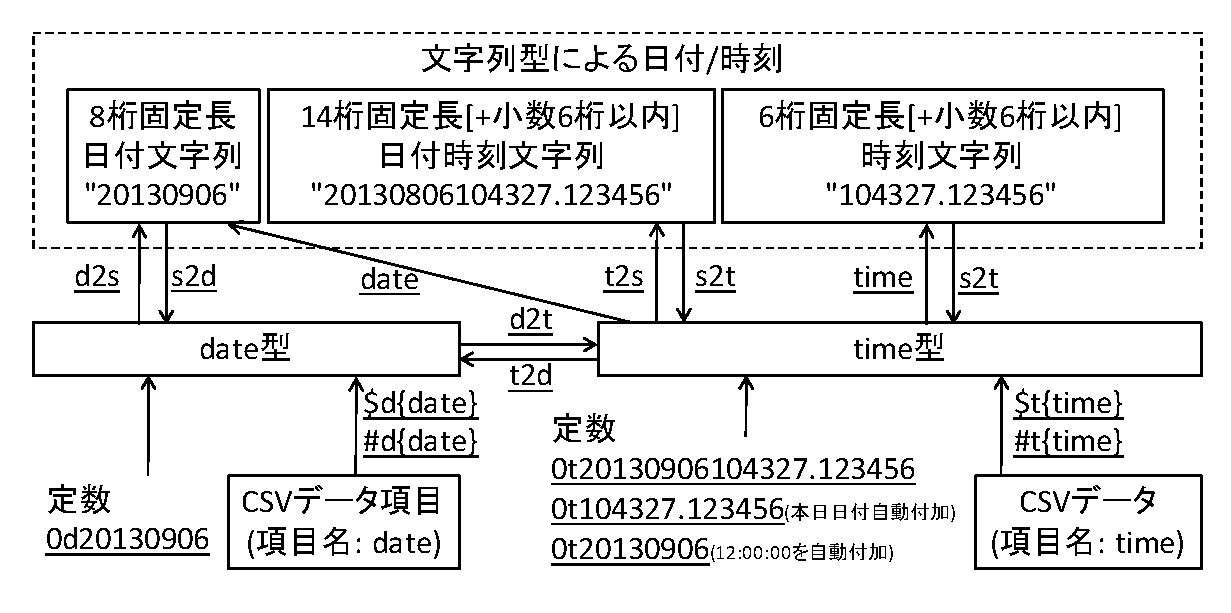
\includegraphics[scale=.50]{figure/datetime/datetime.eps}
\caption{The relationship among time type, date type and various functions using September 6, 2013 at 43 minutes, 27 seconds. The solid line box indicates actual data, the dotted line indicate the functions. \label{fig:mcal_datetime}}
\end{center}
\end{figure}

Other than using fixed length character string as a standard for date/time, user can use Julian day (e.g. continuous count of days since Julian period such as January 1, 4713 BC) or UNIX time (e.g. number of seconds that have elapsed since 00:00:00 Coordinated Universal Time (UTC), Thursday, 1 January 1970) as a signed integer to represent date and time.  The command supports Julian day and UNIX time, as well as conversion functions of date and time data type.   

The mcal command uses an internal date/time format which is based on the Gregorian calendar, thus the date range is limited from January 1,1400 to December 31,9999. Since UNIX time is a signed integer data type of 32 bits, the  furthest time that can be represented this way is 03:14:07 UTC on Tuesday, 19 January 2038, date beyond this point will be interpreted incorrectly due to integer overflow. The drawback of using UNIX time and Julian day is that one will not be able to tell the date and time by looking at the number. 

%\end{document}

%\section{関数リファレンス}

%\begin{document}

\section{abs - Absolute value\label{sect:abs}}
\index{abs@abs}

Format: abs($num$)

Compute absolute value of $num$.

\subsection*{Example}
\subsubsection*{例1: 基本例}



\begin{Verbatim}[baselinestretch=0.7,frame=single]
$ more dat1.csv
id,val
1,1.0
2,-2.5
3,
4,0
$ mcal c='abs(${val})' a=rsl i=dat1.csv o=rsl1.csv
#END# kgcal a=rsl c=abs(${val}) i=dat1.csv o=rsl1.csv
$ more rsl1.csv
id,val,rsl
1,1.0,1
2,-2.5,2.5
3,,
4,0,0
\end{Verbatim}


%\end{document}



%\begin{document}

\section{acos - Inverse Cosine (arccosine)\label{sect:acos}}
\index{acos@acos}

Format: acos($num$)

Compute arccosine (inverse cosine). The function evaluates the principal value ranges of  $-1.0\sim 1.0$, and returns values within the parameter of $0.0\sim \pi$.


\subsection*{Example}
\input{examples/tex/func_acos_ex}

%\end{document}



%\begin{document}

\section{age 年令\label{sect:age}}
\index{age@age}

書式1: age(生年月日,$date$)

書式2: age(生年月日,$time$)

日付$date$(書式1)もしくは時刻$time$(書式2)における年令を返す。
生年月日は書式1,2によって日付型/時刻型を指定する。

\subsection*{利用例}
\subsubsection*{Example 1: Basic Example}

Compute the age from date of birth to a fixed point on calendar on September 1, 2013.


\begin{Verbatim}[baselinestretch=0.7,frame=single]
$ more dat1.csv
id,dob
1,19641010
2,20000101
3,
4,19770812
$ mcal c='age($d{dob},0d20130901)' a=rsl i=dat1.csv o=rsl1.csv
#END# kgcal a=rsl c=age($d{dob},0d20130901) i=dat1.csv o=rsl1.csv
$ more rsl1.csv
id,dob,rsl
1,19641010,48
2,20000101,13
3,,
4,19770812,36
\end{Verbatim}


%\end{document}



%\begin{document}

\section{and 論理積\label{sect:and}}
\index{and@and}

書式: and($bool_1,bool_2,\cdots$)

$bool_i$で与えられた真偽値全ての論理積を計算する。
NULL値を含めた真偽値表は表\ref{tbl:mcal_and}を参照のこと。

\subsection*{利用例}
\subsubsection*{Example 1: Basic Example}



\begin{Verbatim}[baselinestretch=0.7,frame=single]
$ more dat1.csv
id,b1,b2,b3
1,1,0,1
2,1,1,1
3,1,,1
4,1,1,1
$ mcal c='and($b{b1},$b{b2},$b{b3})' a=rsl i=dat1.csv o=rsl1.csv
#END# kgcal a=rsl c=and($b{b1},$b{b2},$b{b3}) i=dat1.csv o=rsl1.csv
$ more rsl1.csv
id,b1,b2,b3,rsl
1,1,0,1,0
2,1,1,1,1
3,1,,1,
4,1,1,1,1
\end{Verbatim}
\subsubsection*{Example 2: Example of using wildcard}

Specify columns names that start with \verb|b| as in (\verb|b1,b2,b3|) using a wildcard in column name such as "\verb|b*|".


\begin{Verbatim}[baselinestretch=0.7,frame=single]
$ mcal c='and($b{b*})' a=rsl i=dat1.csv o=rsl2.csv
#END# kgcal a=rsl c=and($b{b*}) i=dat1.csv o=rsl2.csv
$ more rsl2.csv
id,b1,b2,b3,rsl
1,1,0,1,0
2,1,1,1,1
3,1,,1,
4,1,1,1,1
\end{Verbatim}


%\end{document}



%\begin{document}

\section{argsize 引数の数\label{sect:argsize}}
\index{argsize@argsize}

書式1: argsize($str_1,str_2,\cdots$)

$str_i$で与えられた文字列の数を返す。
ワイルドカードをで項目名を指定することで意味が出てくる。
すなわちワイルドカード条件を満たす多数の項目の数をカウントすることができる。
データ型としては文字列型のみに対応していることに注意する。

\subsection*{利用例}
\subsubsection*{Example 1: Basic Example}

Count the number of column names that start with \verb|"v"|.


\begin{Verbatim}[baselinestretch=0.7,frame=single]
$ more dat1.csv
id,v1,v2,v3
1,1,2,3
2,-5,2,1
3,1,,3
4,,,
$ mcal c='argsize($s{v*})' a=rsl i=dat1.csv o=rsl1.csv
#END# kgcal a=rsl c=argsize($s{v*}) i=dat1.csv o=rsl1.csv
$ more rsl1.csv
id,v1,v2,v3,rsl
1,1,2,3,3
2,-5,2,1,3
3,1,,3,3
4,,,,3
\end{Verbatim}


%\end{document}



%\begin{document}

\section{asin サインの逆関数\label{sect:asin}}
\index{asin@asin}

書式: asin($num$)

アークサイン(サインの逆関数)を計算する。
パラメータの範囲は$-1.0\sim 1.0$で戻り値の範囲は$-\pi/2\sim \pi/2$である。

\subsection*{利用例}
\subsubsection*{Example 1: Basic Example}



\begin{Verbatim}[baselinestretch=0.7,frame=single]
$ more dat1.csv
id,val
1,-1.0
2,0
3,1.0
4,
5,2
$ mcal c='asin(${val})' a=rsl i=dat1.csv o=rsl1.csv
#END# kgcal a=rsl c=asin(${val}) i=dat1.csv o=rsl1.csv
$ more rsl1.csv
id,val,rsl
1,-1.0,-1.570796327
2,0,0
3,1.0,1.570796327
4,,
5,2,
\end{Verbatim}


%\end{document}



%\begin{document}

\section{atan タンジェントの逆関数\label{sect:atan}}
\index{atan@atan}

書式: atan($num$)

アークタンジェント(タンジェントの逆関数)を計算する。
パラメータの範囲は$-\infty\sim \infty$で戻り値の範囲は$-\pi/2 \sim \pi/2$である。

\subsection*{利用例}
\subsubsection*{例1: 基本例}



\begin{Verbatim}[baselinestretch=0.7,frame=single]
$ more dat1.csv
id,val
1,-1.0
2,0
3,1.0
4,
5,1.0e+10
$ mcal c='atan(${val})' a=rsl i=dat1.csv o=rsl1.csv
#END# kgcal a=rsl c=atan(${val}) i=dat1.csv o=rsl1.csv
$ more rsl1.csv
id,val,rsl
1,-1.0,-0.7853981634
2,0,0
3,1.0,0.7853981634
4,,
5,1.0e+10,1.570796327
\end{Verbatim}


%\end{document}



%\begin{document}

\section{atan2 座標の角度\label{sect:atan2}}
\index{atan2@atan2}

書式: atan2($num_1,num_2$)

$x,y$座標$(num_1,num_2)$と原点を結ぶ線分と$x$軸とが作る角度をラジアンで返す。

\subsection*{利用例}
\subsubsection*{例1: 基本例}



\begin{Verbatim}[baselinestretch=0.7,frame=single]
$ more dat1.csv
id,x,y
1,5,10
2,10,20
3,-1,0
4,0,0
5,,
$ mcal c='atan2(${x},${y})' a=rsl i=dat1.csv o=rsl1.csv
#END# kgcal a=rsl c=atan2(${x},${y}) i=dat1.csv o=rsl1.csv
$ more rsl1.csv
id,x,y,rsl
1,5,10,1.107148718
2,10,20,1.107148718
3,-1,0,3.141592654
4,0,0,0
5,,,
\end{Verbatim}


%\end{document}



%\begin{document}

\section{avg 平均\label{sect:avg}}
\index{avg@avg}

書式1: avg($num_1,num_2,\cdots$)

書式2: avg($num_1,num_2,\cdots,str$)

$num_i$で与えられた数値の平均を計算する。
書式1では、NULL値は無視されるが、全てがNULL値であれば結果もNULLとなる。

書式2において最後の引数として"-n"を与えると、
NULL値に対する扱いが変わり、
項目値に一つでもNULL値がある場合は、結果もNULL値となる。

\subsection*{利用例}
\subsubsection*{Example 1: Basic Example}



\begin{Verbatim}[baselinestretch=0.7,frame=single]
$ more dat1.csv
id,v1,v2,v3
1,1,2,3
2,-5,2,1
3,1,,3
4,,,
$ mcal c='avg(${v1},${v2},${v3})' a=rsl i=dat1.csv o=rsl1.csv
#END# kgcal a=rsl c=avg(${v1},${v2},${v3}) i=dat1.csv o=rsl1.csv
$ more rsl1.csv
id,v1,v2,v3,rsl
1,1,2,3,2
2,-5,2,1,-0.6666666667
3,1,,3,2
4,,,,
\end{Verbatim}
\subsubsection*{Example 2: Example of using wildcard}

Specify columns names that start with \verb|v| (\verb|v1,v2,v3|) using a wildcard in column name such as \verb|v*|.


\begin{Verbatim}[baselinestretch=0.7,frame=single]
$ mcal c='avg(${v*})' a=rsl i=dat1.csv o=rsl2.csv
#END# kgcal a=rsl c=avg(${v*}) i=dat1.csv o=rsl2.csv
$ more rsl2.csv
id,v1,v2,v3,rsl
1,1,2,3,2
2,-5,2,1,-0.6666666667
3,1,,3,2
4,,,,
\end{Verbatim}


%\end{document}


%\begin{document}

\section{binomdist 二項分布の累積確率\label{sect:binomdist}}
\index{binomdist@binomdist}

書式: binomdist(成功回数$k$,試行回数$n$,成功確率$p$)

試行回数$n$、成功確率$p$の二項分布$B(n,p)$に従う確率変数$X$について、
累積確率$P[X\le k]$を計算する。
$k,n,p$は、定数としても項目として与えることができる。
なお、$k>n$や$p<0,p>1$の場合の計算結果はnullとなる。

\subsection*{利用例}
\input{examples/tex/func_binomdist_ex}

%\end{document}

 % added from ver.3.0

%\begin{document}

\section{berrand ベルヌーイ乱数\label{sect:berrand}}
\index{berrand@berrand}

書式: berrand(確率[, 乱数の種])

ベルヌーイ分布$f(x)=p^x(1-p)^{1-x} x=0,1$について、指定された確率$p$における$x$の乱数を生成する。
本関数では、$x=0$をfalse、$x=1$をtrueとした論理型として値を返す。
また確率$p$は定数としてのみ指定可能で、項目名を指定することはできない。

同じ乱数の種を指定すれば、同じ乱数系列となる。
指定可能な乱数の種の範囲は-2147483648〜2147483647である。
乱数の種を省略すると、
時刻(1/1000秒単位)に応じた異なる乱数の種が利用される。

乱数の生成にはメルセンヌ・ツイスター法を利用している
(\href{http://www.math.sci.hiroshima-u.ac.jp/~m-mat/MT/emt.html}{原作者のページ}
, \href{http://www.boost.org/doc/libs/1_54_0/doc/html/boost_random.html}{boostライブラリ})。

\subsection*{利用例}
\input{examples/tex/func_berrand_ex}

%\end{document}

 % added from ver.3.0

%\begin{document}

\section{bottom - Last row\label{sect:bottom}}
\index{bottom@bottom}

Format: bottom()

Return true if record is positioned in the last row, otherwise return false. 


\subsection*{Example}
\subsubsection*{Example 1: Basic Example}



\begin{Verbatim}[baselinestretch=0.7,frame=single]
$ more dat1.csv
val
1
2
3
4
$ mcal c='bottom()' a=rsl i=dat1.csv o=rsl1.csv
#END# kgcal a=rsl c=bottom() i=dat1.csv o=rsl1.csv
$ more rsl1.csv
val,rsl
1,0
2,0
3,0
4,1
\end{Verbatim}


%\end{document}



%\begin{document}

\section{capitalize 先頭文字大文字変換\label{sect:capitalize}}
\index{capitalize@capitalize}

書式: capitalize($str$)

文字列の先頭文字のみ大文字に変更する。 
アルファベット26文字以外の文字については何の影響もない。

\subsection*{利用例}
\subsubsection*{例1: 基本例}

$str$項目の先頭文字を大文字に変換する。


\begin{Verbatim}[baselinestretch=0.7,frame=single]
$ more dat1.csv
id,str
1,abc
2,aBd
3,
4,#abc
$ mcal c='capitalize($s{str})' a=rsl i=dat1.csv o=rsl1.csv
#END# kgcal a=rsl c=capitalize($s{str}) i=dat1.csv o=rsl1.csv
$ more rsl1.csv
id,str,rsl
1,abc,Abc
2,aBd,ABd
3,,
4,#abc,#abc
\end{Verbatim}


%\end{document}



%\begin{document}

\section{cat - Concatenate Character String\label{sect:cat}}
\index{cat@cat}

Format: cat($token,str_1,str_2,\cdots$)

Concatenate the specified $str_i$ in order using $token$ as the delimiter to create a character string. If an empty character \verb|""| is specified, the list of strings are simply concatenated. 


\subsection*{Examples}
\subsubsection*{例1: 基本例}

3つの項目str1,str2,str3を\verb|"#"|の区切り文字を挿入して併合する。


\begin{Verbatim}[baselinestretch=0.7,frame=single]
$ more dat1.csv
id,str1,str2,str3
1,abc,def,ghi
2,A,,CDE
3,,,
4,,,XY
$ mcal c='cat("#",$s{str1},$s{str2},$s{str3})' a=rsl i=dat1.csv o=rsl1.csv
#END# kgcal a=rsl c=cat("#",$s{str1},$s{str2},$s{str3}) i=dat1.csv o=rsl1.csv
$ more rsl1.csv
id,str1,str2,str3,rsl
1,abc,def,ghi,abc#def#ghi
2,A,,CDE,A##CDE
3,,,,##
4,,,XY,##XY
\end{Verbatim}
\subsubsection*{例2: tokenが空文字の場合}



\begin{Verbatim}[baselinestretch=0.7,frame=single]
$ mcal c='cat("",$s{str1},$s{str2},$s{str3})' a=rsl i=dat1.csv o=rsl2.csv
#END# kgcal a=rsl c=cat("",$s{str1},$s{str2},$s{str3}) i=dat1.csv o=rsl2.csv
$ more rsl2.csv
id,str1,str2,str3,rsl
1,abc,def,ghi,abcdefghi
2,A,,CDE,ACDE
3,,,,
4,,,XY,XY
\end{Verbatim}
\subsubsection*{例3: ワイルドカードを利用した例}

\verb|str|から始まる項目(\verb|str1,str2,str3|)をワイルドカード「\verb|str*|」によって指定している。


\begin{Verbatim}[baselinestretch=0.7,frame=single]
$ mcal c='cat("",$s{str*})' a=rsl i=dat1.csv o=rsl3.csv
#END# kgcal a=rsl c=cat("",$s{str*}) i=dat1.csv o=rsl3.csv
$ more rsl3.csv
id,str1,str2,str3,rsl
1,abc,def,ghi,abcdefghi
2,A,,CDE,ACDE
3,,,,
4,,,XY,XY
\end{Verbatim}


%\end{document}



%\begin{document}

\section{ceil - Ceiling\label{sect:ceil}}
\index{ceil@ceil}

Format: ceil($num$,base)

Round up $num$ based on multiples of the base number, and returns the smallest integer that is greater than or equal to $num$. 

For example, given ceil(3.42,05), the numerical value will be rounded up by scales of 0.5 that is greater than 3.42. Thus, the rounded number at base 0.5 becomes 3.5. When base is not specified as an argument, the default base is set at 1. 
This is equivalent to rounding up to the nearest integer after the decimal. 
 

\subsection*{Examples}
\subsubsection*{例1: 基本例}

小数点以下一桁目を切り捨てる。


\begin{Verbatim}[baselinestretch=0.7,frame=single]
$ more dat1.csv
id,val
1,3.28
2,3.82
3,
4,-0.6
$ mcal c='floor(${val})' a=rsl i=dat1.csv o=rsl1.csv
#END# kgcal a=rsl c=floor(${val}) i=dat1.csv o=rsl1.csv
$ more rsl1.csv
id,val,rsl
1,3.28,3
2,3.82,3
3,,
4,-0.6,-1
\end{Verbatim}
\subsubsection*{例2: 基本例}

小数点以下二桁目を切り捨てる。


\begin{Verbatim}[baselinestretch=0.7,frame=single]
$ mcal c='floor(${val},0.1)' a=rsl i=dat1.csv o=rsl2.csv
#END# kgcal a=rsl c=floor(${val},0.1) i=dat1.csv o=rsl2.csv
$ more rsl2.csv
id,val,rsl
1,3.28,3.2
2,3.82,3.8
3,,
4,-0.6,-0.6
\end{Verbatim}
\subsubsection*{例3: 基数0.5の例}

0.5を基数として切り捨てる。


\begin{Verbatim}[baselinestretch=0.7,frame=single]
$ mcal c='floor(${val},0.5)' a=rsl i=dat1.csv o=rsl3.csv
#END# kgcal a=rsl c=floor(${val},0.5) i=dat1.csv o=rsl3.csv
$ more rsl3.csv
id,val,rsl
1,3.28,3
2,3.82,3.5
3,,
4,-0.6,-1
\end{Verbatim}
\subsubsection*{例4: 基数10の例}

一桁目を切り捨てる。


\begin{Verbatim}[baselinestretch=0.7,frame=single]
$ more dat2.csv
id,val
1,1341.28
2,188
3,1.235E+3
4,-1.235E+3
$ mcal c='floor(${val},10)' a=rsl i=dat2.csv o=rsl4.csv
#END# kgcal a=rsl c=floor(${val},10) i=dat2.csv o=rsl4.csv
$ more rsl4.csv
id,val,rsl
1,1341.28,1340
2,188,180
3,1.235E+3,1230
4,-1.235E+3,-1240
\end{Verbatim}


%\end{document}



%\begin{document}

\section{cos - Cosine\label{sect:cos}}
\index{cos@cos}

Format: cos($r$)

Compute radians of $r$ using cosine function. 

\subsection*{Example}
\input{examples/tex/func_cos_ex}

%\end{document}



%\begin{document}

\section{cosh 双曲線余弦\label{sect:cosh}}
\index{cosh@cosh}

書式: cosh($r$)

双曲線余弦 (ハイパーボリック コサイン) を計算する。

\subsection*{利用例}
\subsubsection*{例1: 基本例}



\begin{Verbatim}[baselinestretch=0.7,frame=single]
$ more dat1.csv
id,val
1,3.141592
2,-1.047197
3,
4,6.283185
$ mcal c='cosh(${val})' a=rsl i=dat1.csv o=rsl1.csv
#END# kgcal a=rsl c=cosh(${val}) i=dat1.csv o=rsl1.csv
$ more rsl1.csv
id,val,rsl
1,3.141592,11.59194573
2,-1.047197,1.600286169
3,,
4,6.283185,267.7466792
\end{Verbatim}


%\end{document}



%\begin{document}

\section{countnull 合計\label{sect:countnull}}
\index{countnull@countnull}

書式1: countnull($num_1,num_2,\cdots$)

書式2: countnull($str_1,str_2,\cdots$)

書式3: countnull($date_1,date_2,\cdots$)

書式4: countnull($time_1,time_2,\cdots$)

書式5: countnull($bool_1,bool_2,\cdots$)

$num_i$(その他の型も同様)で与えられた数値の中でNULL値の数を返す。

\subsection*{利用例}
\subsubsection*{Example 1: Basic Example}



\begin{Verbatim}[baselinestretch=0.7,frame=single]
$ more dat1.csv
a,b,c,d
1,,3,4
1,,,
,,,
$ mcal c='countnull(${a},${b},${c},${d})' a=rsl i=dat1.csv o=rsl1.csv
#END# kgcal a=rsl c=countnull(${a},${b},${c},${d}) i=dat1.csv o=rsl1.csv
$ more rsl1.csv
a,b,c,d,rsl
1,,3,4,1
1,,,,3
,,,,4
\end{Verbatim}
\subsubsection*{Example 2: Specify other types of data format in field with wildcard character}



\begin{Verbatim}[baselinestretch=0.7,frame=single]
$ mcal c='countnull($s{*})' a=rsl i=dat1.csv o=rsl2.csv
#END# kgcal a=rsl c=countnull($s{*}) i=dat1.csv o=rsl2.csv
$ more rsl2.csv
a,b,c,d,rsl
1,,3,4,1
1,,,,3
,,,,4
\end{Verbatim}


%\end{document}



%\begin{document}

\section{d2julian: date-Change date to a Julian day\label{sect:d2julian}}
\index{d2julian@d2julian}

Format: d2julian($date$)
Use this function to obtain a Julian day from the date.
\begin{verbatim}
A Julian day is the number of days from noon of January 1, 4713 B.C. (universal time).
The effective range of the Gregorian calendar, however, is 1400-1-1 to 9999-12-31, so the corresponding range of the Julius days is 2232300 to 5373484.
NULL is output if the result is outside the range.
\end{verbatim}

\subsection*{Usage}
\begin{verbatim}
c=d2julian(0d20080822)
\end{verbatim}

\subsection*{Example}

\begin{table}[hbt]
\begin{center}
 \caption{Input data}
  \begin{tabular}{|c|c|c|} \hline
Date&Time&Number\\ \hline\hline
20020824&20020824145408&10660\\ \hline
20020622&20020622173449&22740\\ \hline
20020824&20020824145408&14800\\ \hline
20021009&20021009095743&54510\\ \hline
20020121&20020121173449&18750\\ \hline
  \end{tabular}
  \end{center}
\end{table}

Examples based on the above data are shown below.

\subsubsection*{Execution example1)}
The value in the “Date” field is input and converted into a Julian day. A “Julian day” field is newly created, and the result is output.
\begin{verbatim}
------------------------------------------------
mcal c='d2julian($d{Date})' a="Julian day" i=date.csv o=od2julian.csv
------------------------------------------------
\end{verbatim}

\begin{table}[hbt]
\begin{center}
 \caption{Output file(od2julian.csv)}
  \begin{tabular}{|c|c|c|c|} \hline
Date&Time&Number&Julian day\\ \hline\hline
20020824&20020824145408&10660&2452511\\ \hline
20020622&20020622173449&22740&2452448\\ \hline
20020824&20020824145408&14800&2452511\\ \hline
20021009&20021009095743&54510&2452557\\ \hline
20020121&20020121173449&18750&2452296\\ \hline
  \end{tabular}
  \end{center}
\end{table}

\href{run:hizuke.pdf}{Return to mcal - date related}\\
%\end{document}

 % added from ver.3.0

%\begin{document}

\section{day - Day\label{sect:day}}
\index{day@day}

Format 1: day($date$)

Format 2: day($time$)

Format 3: days($date$)

Format 4: days($time$)


Extract day from $time$ or $date$. The function shown in format 1 and 2 returns the numeric value, the function in format 3 and 4 returns 2-digit fixed-length string.


\subsection*{Examples}
\subsubsection*{Example 1: Basic Example}



\begin{Verbatim}[baselinestretch=0.7,frame=single]
$ more dat1.csv
id,date
1,20000101
2,20121021
3,
4,19770812
$ mcal c='day($d{date})' a=rsl i=dat1.csv o=rsl1.csv
#END# kgcal a=rsl c=day($d{date}) i=dat1.csv o=rsl1.csv
$ more rsl1.csv
id,date,rsl
1,20000101,1
2,20121021,21
3,,
4,19770812,12
\end{Verbatim}
\subsubsection*{Example 2: Time format}



\begin{Verbatim}[baselinestretch=0.7,frame=single]
$ more dat2.csv
id,time
1,20000101000000
2,20121021111213
3,
4,19770812122212
$ mcal c='day($t{time})' a=rsl i=dat2.csv o=rsl2.csv
#END# kgcal a=rsl c=day($t{time}) i=dat2.csv o=rsl2.csv
$ more rsl2.csv
id,time,rsl
1,20000101000000,1
2,20121021111213,21
3,,
4,19770812122212,12
\end{Verbatim}


%\end{document}



%\begin{document}

\section{date - Year Month Day\label{sect:date}}
\index{date@date}

Format: date($time$)

Extract 8-digit fixed length string of Year Month Day (YYYMMDD) from $time$. 

\subsection*{Example}
\subsubsection*{Example 1: Basic Example}



\begin{Verbatim}[baselinestretch=0.7,frame=single]
$ more dat1.csv
id,time
1,20000101000000
2,20121021111213
3,
4,19770812122212
$ mcal c='date($t{time})' a=rsl i=dat1.csv o=rsl1.csv
#END# kgcal a=rsl c=date($t{time}) i=dat1.csv o=rsl1.csv
$ more rsl1.csv
id,time,rsl
1,20000101000000,20000101
2,20121021111213,20121021
3,,
4,19770812122212,19770812
\end{Verbatim}


%\end{document}



%\begin{document}

\section{degree 角度\label{sect:degree}}
\index{degree@degree}

書式: degree($r$)

ラジアン$r$に対応する角度を計算する。

\subsection*{利用例}
\input{examples/tex/func_degree_ex}

%\end{document}



%\begin{document}

\section{diff - Calculate Interval\label{sect:diff}}
\index{diff@diff}

Format 1: diffyear($date_1,date_2$)

Format 2: diffyear($time_1,time_2$)

Format 3: diffmonth($date_1,date_2$)

Format 4: diffmonth($time_1,time_2$)

Format 5: diffday($date_1,date_2$)

Format 6: diffday($time_1,time_2$)

Format 7: diffhour($time_1,time_2$)

Format 8: diffminute($time_1,time_2$)

Format 9: diffsecond($time_1,time_2$)

Format 10: diffusecond($time_1,time_2$)

If the two arguments are date types, compute the interval between $date_1$ and $date_2$ ($date_1$ - $date_2$), where the interval is measured in terms of years (diffyear), months (diffmonth), days (diffday). 
If the two arguments are time types, compute the interval between $time_1$ and $time_2$ ($time_1$ - $time_2$), where the interval is measured in terms of years (diffyear), months (diffmonth), days (diffday), hours (diffhour), minutes (diffminute) , seconds (diffsecond), and microseconds (diffusecond).
Fractions are rounded up.

\subsection*{Examples}
\subsubsection*{例1: 月単位での期間}

\verb|date|項目から2013年9月1日までの経過期間を日数で計算する。


\begin{Verbatim}[baselinestretch=0.7,frame=single]
$ more dat1.csv
id,date
1,19641010
2,20000101
3,20130831
4,20130901
5,20130902
$ mcal c='diffday(0d20130901,$d{date})' a=rsl i=dat1.csv o=rsl1.csv
#END# kgcal a=rsl c=diffday(0d20130901,$d{date}) i=dat1.csv o=rsl1.csv
$ more rsl1.csv
id,date,rsl
1,19641010,17858
2,20000101,4992
3,20130831,1
4,20130901,0
5,20130902,-1
\end{Verbatim}
\subsubsection*{例2: 分単位での期間}

\verb|time|項目から2012年1月1日 00時00分00秒までの経過期間を分単位で計算する。


\begin{Verbatim}[baselinestretch=0.7,frame=single]
$ more dat2.csv
id,time
1,20120101000000
2,20120101011112
3,
4,20111231235000
5,20111231235000.123456
$ mcal c='diffmonth(0t20120101000000,$t{time})' a=rsl i=dat2.csv o=rsl2.csv
#END# kgcal a=rsl c=diffmonth(0t20120101000000,$t{time}) i=dat2.csv o=rsl2.csv
$ more rsl2.csv
id,time,rsl
1,20120101000000,0
2,20120101011112,-1
3,,
4,20111231235000,0
5,20111231235000.123456,0
\end{Verbatim}
\subsubsection*{例3: マイクロ秒単位での期間}

\verb|time|項目から2012年1月1日 00時00分00秒までの経過期間を秒単位およびマイクロ秒単位で計算する。


\begin{Verbatim}[baselinestretch=0.7,frame=single]
$ mcal c='diffsecond(0t20120101000000,$t{time})' a=rsl i=dat2.csv o=rsl3.csv
#END# kgcal a=rsl c=diffsecond(0t20120101000000,$t{time}) i=dat2.csv o=rsl3.csv
$ more rsl3.csv
id,time,rsl
1,20120101000000,0
2,20120101011112,-4272
3,,
4,20111231235000,600
5,20111231235000.123456,599
$ mcal c='diffusecond(0t20120101000000,$t{time})' a=rsl i=dat2.csv o=rsl4.csv
#END# kgcal a=rsl c=diffusecond(0t20120101000000,$t{time}) i=dat2.csv o=rsl4.csv
$ more rsl4.csv
id,time,rsl
1,20120101000000,0
2,20120101011112,-4272
3,,
4,20111231235000,600
5,20111231235000.123456,599.876544
\end{Verbatim}


%\end{document}



%\begin{document}

\section{dist - Distance\label{sect:dist}}
\index{dist@dist}

Format: dist(type,$num_1,num_2,\cdots,n_k,num_{k+1},num_{k+2},\cdots,num_{2k}$)

Compute the distance between two dimension vectors ($num_1,num_2,\cdots,n_k),(num_{k+1},num_{k+2},\cdots,num_{2k}$). Refer to \verb|msim| for detailed definitions.


\begin{itemize}
\item \verb|euclid|: Euclidean distance 
\item \verb|cityblock|: City Block distance 
\item \verb|hamming|: Hamming distance
\end{itemize}


Hamming distance must be specified in character string format(refer to the example below). 

\subsection*{Examples}
\subsubsection*{例1: ユークリッド距離}



\begin{Verbatim}[baselinestretch=0.7,frame=single]
$ more dat1.csv
id,x1,y1,x2,y2
1,0,0,1,1
2,0,1,2,0
3,,,,
$ mcal c='dist("euclid",${x1},${y1},${x2},${y2})' a=rsl i=dat1.csv o=rsl1.csv
#END# kgcal a=rsl c=dist("euclid",${x1},${y1},${x2},${y2}) i=dat1.csv o=rsl1.csv
$ more rsl1.csv
id,x1,y1,x2,y2,rsl
1,0,0,1,1,1.414213562
2,0,1,2,0,2.236067977
3,,,,,
\end{Verbatim}
\subsubsection*{例2: 都市ブロック距離}



\begin{Verbatim}[baselinestretch=0.7,frame=single]
$ mcal c='dist("cityblock",${x1},${y1},${x2},${y2})' a=rsl i=dat1.csv o=rsl2.csv
#END# kgcal a=rsl c=dist("cityblock",${x1},${y1},${x2},${y2}) i=dat1.csv o=rsl2.csv
$ more rsl2.csv
id,x1,y1,x2,y2,rsl
1,0,0,1,1,2
2,0,1,2,0,3
3,,,,,
\end{Verbatim}
\subsubsection*{例3: ハミング距離}

ハミング距離の計算では、値を文字列として指定していることに注意する。


\begin{Verbatim}[baselinestretch=0.7,frame=single]
$ more dat2.csv
id,x1,y1,x2,y2
1,a,b,a,c
2,0,1,0,1
3,,,,
$ mcal c='dist("hamming",$s{x1},$s{y1},$s{x2},$s{y2})' a=rsl i=dat2.csv o=rsl3.csv
#END# kgcal a=rsl c=dist("hamming",$s{x1},$s{y1},$s{x2},$s{y2}) i=dat2.csv o=rsl3.csv
$ more rsl3.csv
id,x1,y1,x2,y2,rsl
1,a,b,a,c,1
2,0,1,0,1,2
3,,,,,
\end{Verbatim}


%\end{document}



%\documentclass{article}
%\begin{document} 

\section{distgps - GPS Distance\label{sect:distgps}}
\index{distgps@distgps}

Format: distgps(latitude1,longitude1,latitude2,longitude2[,orientation])

Find out the straight-line / direct distance (km unit) between two points based on the latitude and longtitude coordinates. The latitude and longitude can be expressed in signed decimal degrees without compass direction, where positive indicates north/east, negative indicates west/south, on the basis of a spherical earth.  The latitude and longtitude is represent in heading of 60 degrees, and the format is expressed as degree, minute, second ($d,m,s$). The values must be converted to base of 10 for use with this function. 
Base of 10 coordinates can be calculated by $d+m/60+s/60/60$.  

For example, the distance between Osaka (north latitude 34.702398,east longitude 135.495188) and Tokyo (north latitude 35.681391,east longitude 139.766103) is calculated as follows. 

\begin{verbatim}
distgps(34.702398,135.495188,35.681391,139.766103)
\end{verbatim}
In addition, the distance from Everest (north latitude 32.655556,east longitude 79.015833) to Aconcagua (southern latitude 27.987778,west longitude 86.944444) is specified as follows. 
\begin{verbatim}
distgps(32.655556,79.015833,-27.987778,-86.944444)
\end{verbatim}

%Fuji        & 35$^\circ$21'38"N & 138-43-39E & 35.360628N & 138.727365E
%Kilimanjaro & 03$^\circ$04'33"S &  37-21-12E &  3.07583S  &  37.35333E
%Denali      & 63-4-10N  & 151-0-26W 
%Aconcagua   & 32.39.20S & 79.00.57W

\subsection*{Example}
\subsubsection*{Example 1: Basic Example}



\begin{Verbatim}[baselinestretch=0.7,frame=single]
$ more dat1.csv
point1,point2,lat1,lon1,lat2,lon2
osaka,tenma,34.702398,135.495188,34.704923,135.512233
osaka,tokyo,34.702398,135.495188,35.681391,139.766103
osaka,kobe,34.702398,135.495188,34.679453,135.178221
osaka,Fuji,34.702398,135.495188,35.360556,138.727500
Evelest,Aconcagua,32.655556,79.015833,-27.987778,-86.944444
Denali,Kilimanjaro,63.069444,-151.007222,-3.075833,37.353333
$ mcal c='distgps(${lat1},${lon1},${lat2},${lon2})' a=rsl i=dat1.csv o=rsl1.csv
#END# kgcal a=rsl c=distgps(${lat1},${lon1},${lat2},${lon2}) i=dat1.csv o=rsl1.csv
$ more rsl1.csv
point1,point2,lat1,lon1,lat2,lon2,rsl
osaka,tenma,34.702398,135.495188,34.704923,135.512233,1.585046048
osaka,tokyo,34.702398,135.495188,35.681391,139.766103,405.774306
osaka,kobe,34.702398,135.495188,34.679453,135.178221,29.12042213
osaka,Fuji,34.702398,135.495188,35.360556,138.727500,304.7527532
Evelest,Aconcagua,32.655556,79.015833,-27.987778,-86.944444,16956.12242
Denali,Kilimanjaro,63.069444,-151.007222,-3.075833,37.353333,11362.37758
\end{Verbatim}


%\end{document}



%\begin{document}

\section{dow 曜日\label{sect:dow}}
\index{dow@dow}

書式1: dow($date$) 曜日番号(1〜7)

書式2: dow($time$) 曜日番号(1〜7)

書式3: dowj($date$) 日本語曜日

書式4: dowj($time$) 日本語曜日

書式5: dowe($date$) 英語曜日

書式6: dowe($time$) 英語曜日

書式7: dowes($date$) 英語短縮曜日

書式8: dowes($time$) 英語短縮曜日

日付$date$もしくは時刻$time$から曜日を返す。
曜日の表記によって書式1〜8を使い分ける。
曜日番号は、ISO8601の規定に従い、1が月曜日で7が日曜日に対応する。
\subsection*{利用例}
\subsubsection*{例1: 基本例}



\begin{Verbatim}[baselinestretch=0.7,frame=single]
$ more dat1.csv
id,date
1,20000101
2,20121021
3,
4,19770812
$ mcal c='dow($d{date})' a=rsl i=dat1.csv o=rsl1.csv
#END# kgcal a=rsl c=dow($d{date}) i=dat1.csv o=rsl1.csv
$ more rsl1.csv
id,date,rsl
1,20000101,6
2,20121021,7
3,,
4,19770812,5
\end{Verbatim}
\subsubsection*{例2: 日本語表記}



\begin{Verbatim}[baselinestretch=0.7,frame=single]
$ mcal c='dowj($d{date})' a=rsl i=dat1.csv o=rsl2.csv
#END# kgcal a=rsl c=dowj($d{date}) i=dat1.csv o=rsl2.csv
$ more rsl2.csv
id,date,rsl
1,20000101,土
2,20121021,日
3,,
4,19770812,金
\end{Verbatim}
\subsubsection*{例3: 英語表記}



\begin{Verbatim}[baselinestretch=0.7,frame=single]
$ mcal c='dowe($d{date})' a=rsl i=dat1.csv o=rsl3.csv
#END# kgcal a=rsl c=dowe($d{date}) i=dat1.csv o=rsl3.csv
$ more rsl3.csv
id,date,rsl
1,20000101,Saturday
2,20121021,Sunday
3,,
4,19770812,Friday
\end{Verbatim}
\subsubsection*{例4: 英語短縮表記}



\begin{Verbatim}[baselinestretch=0.7,frame=single]
$ mcal c='dowes($d{date})' a=rsl i=dat1.csv o=rsl4.csv
#END# kgcal a=rsl c=dowes($d{date}) i=dat1.csv o=rsl4.csv
$ more rsl4.csv
id,date,rsl
1,20000101,Sat
2,20121021,Sun
3,,
4,19770812,Fri
\end{Verbatim}
\subsubsection*{例5: 時刻型でも可能}



\begin{Verbatim}[baselinestretch=0.7,frame=single]
$ more dat2.csv
id,time
1,20000101000000
2,20121021111213
3,
4,19770812122212
$ mcal c='dow($t{time})' a=rsl i=dat2.csv o=rsl5.csv
#END# kgcal a=rsl c=dow($t{time}) i=dat2.csv o=rsl5.csv
$ more rsl5.csv
id,time,rsl
1,20000101000000,6
2,20121021111213,7
3,,
4,19770812122212,5
\end{Verbatim}


%\end{document}



%\begin{document}

\section{e - Napier’s Constant\label{sect:e}}
\index{e@e}

Format: e()

Return Napier’s Constant ($e$).

\subsection*{Example}
\subsubsection*{例1: 基本例}



\begin{Verbatim}[baselinestretch=0.7,frame=single]
$ more dat1.csv
id
1
2
$ mcal c='e()' a=rsl i=dat1.csv o=rsl1.csv
#END# kgcal a=rsl c=e() i=dat1.csv o=rsl1.csv
$ more rsl1.csv
id,rsl
1,2.718281828
2,2.718281828
\end{Verbatim}


%\end{document}



%\begin{document}

\section{exp 指数関数\label{sect:exp}}
\index{exp@exp}

書式: exp($num$)

power関数の特殊形で、$e$(ネイピア数)を底とする$num$乗を計算する。

\subsection*{利用例}

\subsubsection*{例1: 基本例}


\begin{Verbatim}[baselinestretch=0.7,frame=single]
$ cat dat1.csv
id,exponent
1,1
2,-1
3,
4,0
5,0.5

$ mcal c='exp(${exponent})' a=rsl i=dat1.csv o=rsl1.csv
#END# kgcal a=rsl c=exp(${exponent}) i=dat1.csv o=rsl1.csv

$ cat rsl1.csv
id,exponent,rsl
1,1,2.718281828
2,-1,0.3678794412
3,,
4,0,1
5,0.5,1.648721271
\end{Verbatim}


%\end{document}


%\begin{document}

\section{factorial 階乗\label{sect:factorial}}
\index{factorial@factorial}

書式: factorial($num$)

$num$の階乗を計算する。
結果が実数の最大値を超えると、NULL値が出力される。

\subsection*{利用例}
\subsubsection*{Example 1: Basic Example}



\begin{Verbatim}[baselinestretch=0.7,frame=single]
$ more dat1.csv
id,val
1,1
2,5
3,
4,10000
$ mcal c='factorial(${val})' a=rsl i=dat1.csv o=rsl1.csv
#END# kgcal a=rsl c=factorial(${val}) i=dat1.csv o=rsl1.csv
$ more rsl1.csv
id,val,rsl
1,1,1
2,5,120
3,,
4,10000,
\end{Verbatim}
\subsubsection*{Example 2: Example of using constants}

Calculate the factorial of 5. When constants is used as an argument, all rows will return the same result.


\begin{Verbatim}[baselinestretch=0.7,frame=single]
$ mcal c='factorial(5)' a=rsl i=dat1.csv o=rsl2.csv
#END# kgcal a=rsl c=factorial(5) i=dat1.csv o=rsl2.csv
$ more rsl2.csv
id,val,rsl
1,1,120
2,5,120
3,,120
4,10000,120
\end{Verbatim}


%\end{document}


%\begin{document}

\section{fixlen 固定長変換\label{sect:fixlen}}
\index{fixlen@fixlen}

書式1: fixlen($str$,長さ,位置,padding文字)

書式2: fixlenw($str$,長さ,位置,padding文字)

$str$を固定の長さの文字列に変換する。
$str$が指定の長さに満たない場合は、
右詰もしくは左詰めで指定した文字を埋め込む。
左右の選択では、「位置」パラメータに\verb|"L"|もしくは\verb|"R"|を指定する。
埋め込む文字は「padding文字」パラメータに任意の文字を指定する。
また、$str$の長さが、指定した固定長の長さを超えた場合、
右詰の場合は先頭側が、左詰めの場合は末尾側の文字列が削られることに注意する。

マルチバイト文字を対象とした固定長変換については\verb|fixlenw|関数を利用する。

\subsection*{利用例}
\subsubsection*{Example 1: Basic Example}

Convert values in the \verb|str| column to 5 character fixed-length string. Right justified (\verb|"R"|) the strings and fill the empty positions with \verb|"#"| for strings with less than 5 characters.


\begin{Verbatim}[baselinestretch=0.7,frame=single]
$ more dat1.csv
id,str
1,abc
2,123
3,
4,1234567
$ mcal c='fixlen($s{str},5,"R","#")' a=rsl i=dat1.csv o=rsl1.csv
#END# kgcal a=rsl c=fixlen($s{str},5,"R","#") i=dat1.csv o=rsl1.csv
$ more rsl1.csv
id,str,rsl
1,abc,##abc
2,123,##123
3,,#####
4,1234567,34567
\end{Verbatim}
\subsubsection*{Example 2: Left justified}

Fill empty positions for left justified (\verb|"L"|) text with \verb|"#"|.


\begin{Verbatim}[baselinestretch=0.7,frame=single]
$ mcal c='fixlen($s{str},5,"L","#")' a=rsl i=dat1.csv o=rsl2.csv
#END# kgcal a=rsl c=fixlen($s{str},5,"L","#") i=dat1.csv o=rsl2.csv
$ more rsl2.csv
id,str,rsl
1,abc,abc##
2,123,123##
3,,#####
4,1234567,12345
\end{Verbatim}
\subsubsection*{Example 3: Multibyte string}



\begin{Verbatim}[baselinestretch=0.7,frame=single]
$ more dat2.csv
id,str
1,こんにちは
2,大阪
$ mcal c='fixlenw($s{str},4,"R","埋")' a=rsl i=dat2.csv o=rsl3.csv
#END# kgcal a=rsl c=fixlenw($s{str},4,"R","埋") i=dat2.csv o=rsl3.csv
$ more rsl3.csv
id,str,rsl
1,こんにちは,んにちは
2,大阪,埋埋大阪
\end{Verbatim}


%\end{document}



%\begin{document}

\section{fldsize - Number of Fields\label{sect:fldsize}}
\index{fldsize@fldsize}

Format: fldsize()

Return the number of fields in the input file. 
MCMD assumes all records in the input data has same number of fields, thus the resulting value from the function applies to all records. 


\subsection*{Examples}
\subsubsection*{Example 1: Basic Example}



\begin{Verbatim}[baselinestretch=0.7,frame=single]
$ more dat1.csv
a,b,c,d
1,2,3,4
2,3,4,5
3,,,
4,x,y,z
$ mcal c='fldsize()' a=rsl i=dat1.csv o=rsl1.csv
#END# kgcal a=rsl c=fldsize() i=dat1.csv o=rsl1.csv
$ more rsl1.csv
a,b,c,d,rsl
1,2,3,4,4
2,3,4,5,4
3,,,,4
4,x,y,z,4
\end{Verbatim}


%\end{document}



%\begin{document}

\section{floor - Rounding Down\label{sect:floor}}
\index{floor@floor}

Format: floor($num$,base)

Round $num$ down to the nearest integer.  This function round down to the maximum integer that is not greater than $num$. For example, in the argument floor(3.82,0.5), the decimal point of 3.82 is above the scale point of 0.5, thus, rounding down to the nearest 0.5 base returns 3.5. The default value of base is 1 if the argument is not defined. This is equivalent to rounding to an integer value by truncating all decimal digits. 


\subsection*{Examples}
\subsubsection*{例1: 基本例}

小数点以下一桁目を切り捨てる。


\begin{Verbatim}[baselinestretch=0.7,frame=single]
$ more dat1.csv
id,val
1,3.28
2,3.82
3,
4,-0.6
$ mcal c='floor(${val})' a=rsl i=dat1.csv o=rsl1.csv
#END# kgcal a=rsl c=floor(${val}) i=dat1.csv o=rsl1.csv
$ more rsl1.csv
id,val,rsl
1,3.28,3
2,3.82,3
3,,
4,-0.6,-1
\end{Verbatim}
\subsubsection*{例2: 基本例}

小数点以下二桁目を切り捨てる。


\begin{Verbatim}[baselinestretch=0.7,frame=single]
$ mcal c='floor(${val},0.1)' a=rsl i=dat1.csv o=rsl2.csv
#END# kgcal a=rsl c=floor(${val},0.1) i=dat1.csv o=rsl2.csv
$ more rsl2.csv
id,val,rsl
1,3.28,3.2
2,3.82,3.8
3,,
4,-0.6,-0.6
\end{Verbatim}
\subsubsection*{例3: 基数0.5の例}

0.5を基数として切り捨てる。


\begin{Verbatim}[baselinestretch=0.7,frame=single]
$ mcal c='floor(${val},0.5)' a=rsl i=dat1.csv o=rsl3.csv
#END# kgcal a=rsl c=floor(${val},0.5) i=dat1.csv o=rsl3.csv
$ more rsl3.csv
id,val,rsl
1,3.28,3
2,3.82,3.5
3,,
4,-0.6,-1
\end{Verbatim}
\subsubsection*{例4: 基数10の例}

一桁目を切り捨てる。


\begin{Verbatim}[baselinestretch=0.7,frame=single]
$ more dat2.csv
id,val
1,1341.28
2,188
3,1.235E+3
4,-1.235E+3
$ mcal c='floor(${val},10)' a=rsl i=dat2.csv o=rsl4.csv
#END# kgcal a=rsl c=floor(${val},10) i=dat2.csv o=rsl4.csv
$ more rsl4.csv
id,val,rsl
1,1341.28,1340
2,188,180
3,1.235E+3,1230
4,-1.235E+3,-1240
\end{Verbatim}


%\end{document}


%\begin{document}

\section{format - Formatted Output\label{sect:format}}
\index{format@format}

Format: format($num$, output format)

mcal internally manages floating point numbers. This function changes the output format of the number by specifying the output format available in the C language printf function. The 3 available formats are as follows. 

\begin{itemize}
\item \%f: Decimal format
\item \%e,\%E: Exponent format (Specify \%E to use uppercase E as exponent notation)
\item \%g,\%G: Automatically select output format of f or e (Specify \%G for uppercase notation)
\end{itemize}

For example, the decimal format is expressed as \verb|0.00726| can be expressed as \verb|7.260000e-03| in exponent format, similarly, the exponent format of \verb|1265| is represented as \verb|1.265000e+03|. 

By specifying the \verb|%| or plus sign after the number, the function formats the decimal digits and characters. The number format can be specified in the format of “\verb|whole number.decimal|”. For example, the number \verb|123.456789| with the format specifier of \verb|%5.2f| becomes \verb|123.46|, and the format specifier of \verb|%8.3f| print number as \verb|123.458| with a floating point of 8 characters and 3 characters after decimal. 

Add a plus sign before the number to display the plus sign before the number. For example, \verb|123.456789| with the format specifier of \verb|%+5.2f| format the number as \verb|+123.46|. 

Besides the format highlighted above, it is possible to include any character string in the format. For example, the number \verb|250| can be formatted as \verb|“Total 250 Yen”| using the format specifier of “Total %g Yen”. Use the format specifier of “%%” to display the symbol \%. The number \verb|15| can be formatted as \verb|15%| using the format specifier of \verb|"%g%%"|.    



\subsection*{Examples}
\subsubsection*{例1: 基本例}

\verb|val|を実数として小数点以下2桁に変換する。


\begin{Verbatim}[baselinestretch=0.7,frame=single]
$ more dat1.csv
id,val
1,0.00726
2,123.456789
3,
4,-0.335
$ mcal c='format(${val},"%8.3f")' a=rsl i=dat1.csv o=rsl1.csv
#END# kgcal a=rsl c=format(${val},"%8.3f") i=dat1.csv o=rsl1.csv
$ more rsl1.csv
id,val,rsl
1,0.00726,   0.007
2,123.456789, 123.457
3,,
4,-0.335,  -0.335
\end{Verbatim}
\subsubsection*{例2: 指数表現}

\verb|val|を指数表現で出力。


\begin{Verbatim}[baselinestretch=0.7,frame=single]
$ mcal c='format(${val},"%e")' a=rsl i=dat1.csv o=rsl2.csv
#END# kgcal a=rsl c=format(${val},"%e") i=dat1.csv o=rsl2.csv
$ more rsl2.csv
id,val,rsl
1,0.00726,7.260000e-03
2,123.456789,1.234568e+02
3,,
4,-0.335,-3.350000e-01
\end{Verbatim}


%\end{document}



%\begin{document}

\section{fract - Fractional Part\label{sect:fract}}
\index{fract@fract}

Format: fract($num$)

Returns the fractional part of $num$. Fractions of values in scientific notation will be output as is. 


\subsection*{Example}
\subsubsection*{Example 1: Basic Example}



\begin{Verbatim}[baselinestretch=0.7,frame=single]
$ more dat1.csv
id,val
1,3.14
2,3
3,
4,-12.56789
5,1.2345e+2
6,1.2345e-10
$ mcal c='fract(${val})' a=rsl i=dat1.csv o=rsl1.csv
#END# kgcal a=rsl c=fract(${val}) i=dat1.csv o=rsl1.csv
$ more rsl1.csv
id,val,rsl
1,3.14,0.14
2,3,0
3,,
4,-12.56789,-0.56789
5,1.2345e+2,0.45
6,1.2345e-10,1.2345e-10
\end{Verbatim}


%\end{document}



%\begin{document}

\section{gcd 最大公約数\label{sect:gcd}}
\index{gcd@gcd}

書式: gcd($num_1,num_2$)

$num_1$と$num_2$の最大公約数を求める。
実数は整数に変換して(切り下げ)実行される。

\subsection*{利用例}
\subsubsection*{例1: 基本例}



\begin{Verbatim}[baselinestretch=0.7,frame=single]
$ more dat1.csv
id,val1,val2
1,12,36
2,6,5
3,,
4,12.1,36.2
$ mcal c='gcd(${val1},${val2})' a=rsl i=dat1.csv o=rsl1.csv
#END# kgcal a=rsl c=gcd(${val1},${val2}) i=dat1.csv o=rsl1.csv
$ more rsl1.csv
id,val1,val2,rsl
1,12,36,12
2,6,5,1
3,,,
4,12.1,36.2,12
\end{Verbatim}
\subsubsection*{例2: 定数を与える例}

val1項目と36の最大公約数を求める。


\begin{Verbatim}[baselinestretch=0.7,frame=single]
$ mcal c='gcd(${val1},36)' a=rsl i=dat1.csv o=rsl2.csv
#END# kgcal a=rsl c=gcd(${val1},36) i=dat1.csv o=rsl2.csv
$ more rsl2.csv
id,val1,val2,rsl
1,12,36,12
2,6,5,6
3,,,
4,12.1,36.2,12
\end{Verbatim}


%\end{document}



%\begin{document}

\section{hasspace - Search Whitespace Characters\label{sect:hasspace}}
\index{hasspace@hasspace}

Format 1: hasspace($str$, length)

Format 2: hasspacew($str$, length)

This function returns true if there is whitespace characters in character string $str$ and false if not. Whitespace characters is represented as ASCII code 0X20 to 0x09-0x0d. The respective ASCII code are represented as: single byte space (0x20), horizontal tab (0x09), new line (0x0a), vertical tabulation (0x0b), new page (0x0c), carriage return (0x0d). Use \verb|hasspacew| to search for multibyte white space character.


\subsection*{Examples}
\subsubsection*{Example 1: Basic Example}

Returns true if \verb|str| column contains white space characters. The first row where \verb|id=1|contains single-byte space character, in addition, the second row where \verb|id=2| contains tab character, thus, these two rows return true. However, records where the function returns false are \verb|id=4| which contains carriage return, and \verb|id=3| which contains double-byte space character.


\begin{Verbatim}[baselinestretch=0.7,frame=single]
$ more dat1.csv
id,str
1,a b
2,ab	c
3,ab c
4,
5,"aa
bb"
$ mcal c='hasspace($s{str})' a=rsl i=dat1.csv o=rsl1.csv
#END# kgcal a=rsl c=hasspace($s{str}) i=dat1.csv o=rsl1.csv
$ more rsl1.csv
id,str,rsl
1,a b,1
2,ab	c,1
3,ab c,0
4,,0
5,"aa
bb",1
\end{Verbatim}
\subsubsection*{Example 2: Multibyte character}

Use \verb|hasspacew| function to detect double character space.


\begin{Verbatim}[baselinestretch=0.7,frame=single]
$ mcal c='hasspacew($s{str})' a=rsl i=dat1.csv o=rsl2.csv
#END# kgcal a=rsl c=hasspacew($s{str}) i=dat1.csv o=rsl2.csv
$ more rsl2.csv
id,str,rsl
1,a b,1
2,ab	c,1
3,ab c,1
4,,0
5,"aa
bb",1
\end{Verbatim}


%\end{document}



%\begin{document}

\section{heron 三角形の面積\label{sect:heron}}
\index{heron@heron}

書式: heron(タイプ,$num_1,num_2,\cdots,n_k,num_{k+1},num_{k+2},\cdots,num_{2k},num_{2k+1},num_{2k+2},\cdots,num_{3k}$)

k次元空間の3点の座標$(num_1,num_2,\cdots,n_k),(num_{k+1},num_{k+2},\cdots,num_{2k)}
,(num_{2k+1},num_{2k+2},\cdots,num_{3k})$によって作られる3角形の面積を計算する。

\subsection*{利用例}

\subsubsection*{例1: 基本例}


\begin{Verbatim}[baselinestretch=0.7,frame=single]
$ cat dat1.csv
id,x1,y1,x2,y2,x3,y3
1,0,0,1,0,0,1
2,0,0,0,2,2,0
4,,,,,,
3,0,0,1,1,2,2

$ mcal c='heron(${x1},${y1},${x2},${y2},${x3},${y3})' a=rsl i=dat1.csv o=rsl1.csv
#END# kgcal a=rsl c=heron(${x1},${y1},${x2},${y2},${x3},${y3}) i=dat1.csv o=rsl1.csv

$ cat rsl1.csv
id,x1,y1,x2,y2,x3,y3,rsl
1,0,0,1,0,0,1,0.5
2,0,0,0,2,2,0,2
4,,,,,,,
3,0,0,1,1,2,2,0
\end{Verbatim}


%\end{document}


%\begin{document}

\section{hour - Hour\label{sect:hour}}
\index{hour@hour}

Format 1: hour($time$) Numerical value

Format 2: hours($time$) 2 digit fixed length string

Extract hour from $time$. The function can be used in different purposes as shown in format 1,2. 


\subsection*{Examples}
\subsubsection*{Example 1: Basic Example}



\begin{Verbatim}[baselinestretch=0.7,frame=single]
$ more dat1.csv
id,time
1,20000101000000
2,20121021111213
3,
4,19770812122212
$ mcal c='hour($t{time})' a=rsl i=dat1.csv o=rsl1.csv
#END# kgcal a=rsl c=hour($t{time}) i=dat1.csv o=rsl1.csv
$ more rsl1.csv
id,time,rsl
1,20000101000000,0
2,20121021111213,11
3,,
4,19770812122212,12
\end{Verbatim}
\subsubsection*{Example 2: Output character string}



\begin{Verbatim}[baselinestretch=0.7,frame=single]
$ mcal c='hours($t{time})' a=rsl i=dat1.csv o=rsl2.csv
#END# kgcal a=rsl c=hours($t{time}) i=dat1.csv o=rsl2.csv
$ more rsl2.csv
id,time,rsl
1,20000101000000,00
2,20121021111213,11
3,,
4,19770812122212,12
\end{Verbatim}


%\end{document}



%\begin{document}

\section{if 条件選択\label{sect:if}}
\index{if@if}

書式: if($bool,num_1,num_2$), if($bool,str_1,str_2$), if($bool,date_1,date_2$),if($bool,time_1,time_2$),if($bool,bool_1,bool_2$)

第1パラメータの値が真であれば第2パラメータを、偽であれば第3パラメータを返す。
第1パラメータがNULL値であればNULL値を返す。
第2パラメータと第3パラメータは同じ型でなくてはならないことに注意する。

\subsection*{利用例}
\subsubsection*{Example 1: Basic Example}

If the value in time column is less than 120000, return "AM", otherwise, return "PM".


\begin{Verbatim}[baselinestretch=0.7,frame=single]
$ more dat1.csv
id,time
1,101215
2,210110
3,
4,120001
$ mcal c='if(${time}<=120000,"AM","PM")' a=ampm i=dat1.csv o=rsl1.csv
#END# kgcal a=ampm c=if(${time}<=120000,"AM","PM") i=dat1.csv o=rsl1.csv
$ more rsl1.csv
id,time,ampm
1,101215,AM
2,210110,PM
3,,
4,120001,PM
\end{Verbatim}
\subsubsection*{Example 2: Different parameter types}

The function returns an error if the character format is different in the second and third parameter.


\begin{Verbatim}[baselinestretch=0.7,frame=single]
$ mcal c='if(${time}<=120000,"am",1)' a=ampm i=dat1.csv o=rsl2.csv
#ERROR# unknown function or operator: if_BSN (kgcal)
$ more rsl2.csv
\end{Verbatim}
\subsubsection*{Example 3: Return boolean value on conditional statements}

Read the value in the column using \verb|$b{fieldname}|, if the value is “1” return true, if it is “0” return false, other values will be treated as NULL.


\begin{Verbatim}[baselinestretch=0.7,frame=single]
$ more dat2.csv
id,val
1,1
2,0
3,
4,-2
$ mcal c='if($b{val},"ture","false")' a=bool i=dat2.csv o=rsl3.csv
#END# kgcal a=bool c=if($b{val},"ture","false") i=dat2.csv o=rsl3.csv
$ more rsl3.csv
id,val,bool
1,1,ture
2,0,false
3,,
4,-2,
\end{Verbatim}
\subsubsection*{Example 4: Time format comparison}



\begin{Verbatim}[baselinestretch=0.7,frame=single]
$ mcal c='if($t{time}<=0t120000,"am","pm")' a=ampm i=dat1.csv o=rsl4.csv
#END# kgcal a=ampm c=if($t{time}<=0t120000,"am","pm") i=dat1.csv o=rsl4.csv
$ more rsl4.csv
id,time,ampm
1,101215,am
2,210110,pm
3,,
4,120001,pm
\end{Verbatim}
\subsubsection*{Example 5: Nested if function}



\begin{Verbatim}[baselinestretch=0.7,frame=single]
$ more dat3.csv
id,val
1,10
2,0
3,-5
4,0
$ mcal c='if(${val}>0,"plus",if(${val}<0,"minus","zero"))' a=sign i=dat3.csv o=rsl5.csv
#END# kgcal a=sign c=if(${val}>0,"plus",if(${val}<0,"minus","zero")) i=dat3.csv o=rsl5.csv
$ more rsl5.csv
id,val,sign
1,10,plus
2,0,zero
3,-5,minus
4,0,zero
\end{Verbatim}


%\end{document}



%\begin{document}

\section{int - Integer\label{sect:int}}
\index{int@int}

Format: int($num$)

Return the integer value of $num$. Plus and minus signs are returned as is.


\subsection*{Example}

\subsubsection*{例1: 基本例}


\begin{Verbatim}[baselinestretch=0.7,frame=single]
$ cat dat1.csv
id,val
1,3.14
2,3
3,
4,-12.56789
5,1.2345e+2
6,1.2345e-10

$ mcal c='int(${val})' a=rsl i=dat1.csv o=rsl1.csv
#END# kgcal a=rsl c=int(${val}) i=dat1.csv o=rsl1.csv

$ cat rsl1.csv
id,val,rsl
1,3.14,3
2,3,3
3,,
4,-12.56789,-12
5,1.2345e+2,123
6,1.2345e-10,0
\end{Verbatim}


%\end{document}



%\begin{document}

\section{match 検索\label{sect:match}}
\index{match@match}

書式1: match(検索文字列,$str_1,str_2,\cdots$)

書式2: matcha(検索文字列,$str_1,str_2,\cdots$)

書式3: matchs(検索文字列,$str_1,str_2,\cdots$)

書式4: matchas(検索文字列,$str_1,str_2,\cdots$)

$str_1,str_2,\cdots$から指定した検索文字列を検索し、
マッチすれば真をマッチしなければ偽を返す。

OR検索かAND検索か、そして完全一致か部分一致かにより、
表\ref{tbl:func_match_cond}に示すとおり異なる関数名を指定する。

\begin{table}[htbp]
\begin{center}
\caption{入力データ\label{tbl:func_match_cond}}
{\small
\begin{tabular}{l|ll}
\hline
& OR検索 & AND検索 \\
\hline
完全一致 & match  & matcha  \\
部分一致 & matchs & matchas \\
\hline
\end{tabular}
}
\end{center}
\end{table}

\verb|match|関数は、指定した検索文字列が、$str_1,str_2,\cdots$のいずれかに完全一致すれば真を返す。
\verb|matcha|関数は、指定した検索文字列が、$str_1,str_2,\cdots$の全てに完全一致すれば真を返す。
\verb|matchs|関数は、指定した検索文字列が、$str_1,str_2,\cdots$のいずれかに部分一致すれば真を返す。
\verb|matchas|関数は、指定した検索文字列が、$str_1,str_2,\cdots$の全てに部分一致すれば真を返す。
NULL値を含めたOR/AND論理演算の真偽値表は表\ref{tbl:mcal_and}を参照のこと。

\subsection*{利用例}
\subsubsection*{Example 1: OR exact match}

Returns true if either column \verb|f1,f2,f3| contains \verb|1|.


\begin{Verbatim}[baselinestretch=0.7,frame=single]
$ more dat1.csv
id,f1,f2,f3
1,1,1,1
2,1,0,1
3,,,
4,1,,1
$ mcal c='match("1",$s{f1},$s{f2},$s{f3})' a=rsl i=dat1.csv o=rsl1.csv
#END# kgcal a=rsl c=match("1",$s{f1},$s{f2},$s{f3}) i=dat1.csv o=rsl1.csv
$ more rsl1.csv
id,f1,f2,f3,rsl
1,1,1,1,1
2,1,0,1,1
3,,,,0
4,1,,1,1
\end{Verbatim}
\subsubsection*{Example 2: AND exact match}

Returns true if columns \verb|f1,f2,f3| contains the character \verb|"1"|.


\begin{Verbatim}[baselinestretch=0.7,frame=single]
$ mcal c='matcha("1",$s{f1},$s{f2},$s{f3})' a=rsl i=dat1.csv o=rsl2.csv
#END# kgcal a=rsl c=matcha("1",$s{f1},$s{f2},$s{f3}) i=dat1.csv o=rsl2.csv
$ more rsl2.csv
id,f1,f2,f3,rsl
1,1,1,1,1
2,1,0,1,0
3,,,,0
4,1,,1,0
\end{Verbatim}
\subsubsection*{Example 3: OR partial match}

Returns true if the character string \verb|ab| exists in either column \verb|s1,s2,s3|.


\begin{Verbatim}[baselinestretch=0.7,frame=single]
$ more dat2.csv
id,s1,s2,s3
1,ab,abx,x
2,abc,xaby,xxab
3,,,
4,#ac,x,x
$ mcal c='matchs("ab",$s{s1},$s{s2},$s{s3})' a=rsl i=dat2.csv o=rsl3.csv
#END# kgcal a=rsl c=matchs("ab",$s{s1},$s{s2},$s{s3}) i=dat2.csv o=rsl3.csv
$ more rsl3.csv
id,s1,s2,s3,rsl
1,ab,abx,x,1
2,abc,xaby,xxab,1
3,,,,0
4,#ac,x,x,0
\end{Verbatim}
\subsubsection*{Example 4: AND partial match}

Returns true if the character string \verb|ab| exists in columns \verb|s1,s2,s3|.


\begin{Verbatim}[baselinestretch=0.7,frame=single]
$ mcal c='matchas("ab",$s{s1},$s{s2},$s{s3})' a=rsl i=dat2.csv o=rsl4.csv
#END# kgcal a=rsl c=matchas("ab",$s{s1},$s{s2},$s{s3}) i=dat2.csv o=rsl4.csv
$ more rsl4.csv
id,s1,s2,s3,rsl
1,ab,abx,x,0
2,abc,xaby,xxab,1
3,,,,0
4,#ac,x,x,0
\end{Verbatim}
\subsubsection*{Example 5: Search for NULL value}

Return true if \verb|str| column contains NULL value.


\begin{Verbatim}[baselinestretch=0.7,frame=single]
$ mcal c='match(nulls(),$s{s1},$s{s2},$s{s3})' a=rsl i=dat2.csv o=rsl5.csv
#END# kgcal a=rsl c=match(nulls(),$s{s1},$s{s2},$s{s3}) i=dat2.csv o=rsl5.csv
$ more rsl5.csv
id,s1,s2,s3,rsl
1,ab,abx,x,0
2,abc,xaby,xxab,0
3,,,,1
4,#ac,x,x,0
\end{Verbatim}


%\end{document}



%\begin{document}

\section{isnull - Evaluate NULL value\label{sect:isnull}}
\index{isnull@isnull}

Format: isnull($num$), isnull($str$), isnull($date$), isnull($time$), isnull($bool$)

Determine whether NULL value is included in the value $num$ (the same applies to other data type). Returns \verb|0b1| (true) if NULL value exists, and \verb|0b0| (false) otherwise.  


\subsection*{Examples}
\subsubsection*{Example 1: Basic Example}



\begin{Verbatim}[baselinestretch=0.7,frame=single]
$ more dat1.csv
id,val
1,a
2,
3,b
$ mcal c='isnull(${val})' a=rsl i=dat1.csv o=rsl1.csv
#END# kgcal a=rsl c=isnull(${val}) i=dat1.csv o=rsl1.csv
$ more rsl1.csv
id,val,rsl
1,a,0
2,,1
3,b,0
\end{Verbatim}
\subsubsection*{Example 2: Specify other field types}



\begin{Verbatim}[baselinestretch=0.7,frame=single]
$ mcal c='isnull($s{val})' a=rsl i=dat1.csv o=rsl2.csv
#END# kgcal a=rsl c=isnull($s{val}) i=dat1.csv o=rsl2.csv
$ more rsl2.csv
id,val,rsl
1,a,0
2,,1
3,b,0
\end{Verbatim}
\subsubsection*{Example 3: Specify null character}



\begin{Verbatim}[baselinestretch=0.7,frame=single]
$ mcal c='isnull("")' a=rsl i=dat1.csv o=rsl3.csv
#END# kgcal a=rsl c=isnull("") i=dat1.csv o=rsl3.csv
$ more rsl3.csv
id,val,rsl
1,a,1
2,,1
3,b,1
\end{Verbatim}


%\end{document}



%\begin{document}

\section{julian ユリウス暦変換\label{sect:julian}}
\index{julian@julian}

書式1: julian($date$)

書式2: julian($time$)

書式3: julian2d($num$)

書式4: julian2t($num$)

書式1,2では、日付$date$もしくは時刻$time$をユリウス通日に変換する。
逆に書式3,4では、ユリウス通日を日付型もしくは時刻型に変換する。
ここで、日付型が与えられたときは、その日の最初の時刻である\verb|00:00:00|として計算される。

\subsection*{利用例}
\subsubsection*{例1: 基本例}

日付型の\verb|date|項目を\verb|julian|関数でユリウス通日に変換し、\verb|julian2d|関数でまたもとに戻す。


\begin{Verbatim}[baselinestretch=0.7,frame=single]
$ more dat1.csv
id,date
1,20000101
2,20121021
3,
4,19700101
$ mcal c='julian($d{date})' a=julian i=dat1.csv o=rsl1.csv
#END# kgcal a=julian c=julian($d{date}) i=dat1.csv o=rsl1.csv
$ more rsl1.csv
id,date,julian
1,20000101,2451545
2,20121021,2456222
3,,
4,19700101,2440588
$ mcal c='julian2d(${julian})' a=date2 i=rsl1.csv o=rsl2.csv
#END# kgcal a=date2 c=julian2d(${julian}) i=rsl1.csv o=rsl2.csv
$ more rsl2.csv
id,date,julian,date2
1,20000101,2451545,20000101
2,20121021,2456222,20121021
3,,,
4,19700101,2440588,19700101
\end{Verbatim}
\subsubsection*{例2: 時刻型も同様}



\begin{Verbatim}[baselinestretch=0.7,frame=single]
$ more dat2.csv
id,time
1,20000101000000
2,20121021111213
3,
4,19700101000100
$ mcal c='julian($t{time})' a=julian i=dat2.csv o=rsl3.csv
#END# kgcal a=julian c=julian($t{time}) i=dat2.csv o=rsl3.csv
$ more rsl3.csv
id,time,julian
1,20000101000000,2451544.5
2,20121021111213,2456221.967
3,,
4,19700101000100,2440587.501
$ mcal c='julian2t(${julian})' a=time2 i=rsl3.csv o=rsl4.csv
#END# kgcal a=time2 c=julian2t(${julian}) i=rsl3.csv o=rsl4.csv
$ more rsl4.csv
id,time,julian,time2
1,20000101000000,2451544.5,20000101000000
2,20121021111213,2456221.967,20121021111228.800015
3,,,
4,19700101000100,2440587.501,19700101000126.400014
\end{Verbatim}


%\end{document}



%\begin{document}

\section{lcm - Least Common Denominator\label{sect:lcm}}
\index{lcm@lcm}

Format: lcm($num_1,num_2$)

Find out the least common denominator between $num_1$ and $num_2$ .  Real number will be rounded down to whole number.


\subsection*{Examples}

\subsubsection*{例1: 基本例}


\begin{Verbatim}[baselinestretch=0.7,frame=single]
$ cat dat1.csv
id,val1,val2
1,5,3
2,12,4
3,,
4,5.1,3.1

$ mcal c='lcm(${val1},${val2})' a=rsl i=dat1.csv o=rsl1.csv
#END# kgcal a=rsl c=lcm(${val1},${val2}) i=dat1.csv o=rsl1.csv

$ cat rsl1.csv
id,val1,val2,rsl
1,5,3,15
2,12,4,12
3,,,
4,5.1,3.1,15
\end{Verbatim}

\subsubsection*{例2: 定数を与える例}

val1項目と15の最小公倍数を求める。

\begin{Verbatim}[baselinestretch=0.7,frame=single]
$ mcal c='lcm(${val1},15)' a=rsl i=dat1.csv o=rsl2.csv
#END# kgcal a=rsl c=lcm(${val1},15) i=dat1.csv o=rsl2.csv

$ cat rsl2.csv
id,val1,val2,rsl
1,5,3,15
2,12,4,60
3,,,
4,5.1,3.1,15
\end{Verbatim}


%\end{document}



%\begin{document}

\section{leapyear 閏年判定\label{sect:leapyear}}
\index{leapyear@leapyear}

書式1: leapyear($date$)

書式2: leapyear($time$)

日付$date$もしくは時刻$time$が閏年かどうか判定する。

\subsection*{利用例}
\input{examples/tex/func_leapyear_ex}

%\end{document}



%\begin{document}

\section{left 先頭切り出し\label{sect:left}}
\index{left@left}

書式1: left($str$, 長さ)

書式2: leftw($str$, 長さ)

文字列$str$について先頭から長さパラメータで指定した文字数を切り出す。
マルチバイト文字を含む場合はleftwを使うこと。

\subsection*{利用例}
\subsubsection*{例1: 基本例}

str項目の先頭から3文字を切り出す。


\begin{Verbatim}[baselinestretch=0.7,frame=single]
$ more dat1.csv
id,str
1,abcdefg
2,12345678
3,
4,12
$ mcal c='left($s{str},3)' a=rsl i=dat1.csv o=rsl1.csv
#END# kgcal a=rsl c=left($s{str},3) i=dat1.csv o=rsl1.csv
$ more rsl1.csv
id,str,rsl
1,abcdefg,abc
2,12345678,123
3,,
4,12,12
\end{Verbatim}
\subsubsection*{例2: マルチバイト文字を含む例}

マルチバイト文字を含む場合はleftwを使う。


\begin{Verbatim}[baselinestretch=0.7,frame=single]
$ more dat2.csv
id,str
1,あいうえお
2,1あ2345678
3,1あ
4,ああ
$ mcal c='leftw($s{str},3)' a=rsl i=dat2.csv o=rsl2.csv
#END# kgcal a=rsl c=leftw($s{str},3) i=dat2.csv o=rsl2.csv
$ more rsl2.csv
id,str,rsl
1,あいうえお,あいう
2,1あ2345678,1あ2
3,1あ,1あ
4,ああ,ああ
\end{Verbatim}


%\end{document}



%\begin{document}

\section{length 文字列長\label{sect:length}}
\index{length@length}

書式1: length($str$)

書式2: lengthw($str$)

文字列の長さを計算する。
lengthw関数を用いると、$str$をワイド文字として扱う。
NULL値の長さは0であることに注意する。

\subsection*{利用例}
\subsubsection*{例1: 基本例}



\begin{Verbatim}[baselinestretch=0.7,frame=single]
$ more dat1.csv
id,str
1,abc
2,3.1415
3,
4,hello world!
$ mcal c='length($s{str})' a=rsl i=dat1.csv o=rsl1.csv
#END# kgcal a=rsl c=length($s{str}) i=dat1.csv o=rsl1.csv
$ more rsl1.csv
id,str,rsl
1,abc,3
2,3.1415,6
3,,0
4,hello world!,12
\end{Verbatim}
\subsubsection*{例2: マルチバイト文字を含む例}

以下はutf-8でエンコーディングされた日本語を用いた例である。
utf-8の日本語は1文字3バイトでエンコーディングされているので、
length関数では日本語としての文字数ではなく、そのバイト数を返す。


\begin{Verbatim}[baselinestretch=0.7,frame=single]
$ more dat2.csv
id,str
1,こんにちは
2,大阪
$ mcal c='length($s{str})' a=rsl i=dat2.csv o=rsl2.csv
#END# kgcal a=rsl c=length($s{str}) i=dat2.csv o=rsl2.csv
$ more rsl2.csv
id,str,rsl
1,こんにちは,15
2,大阪,6
\end{Verbatim}
\subsubsection*{例3: ワイド文字として扱う例}

lengthwを使うと、内部で文字列をワイド文字に変換するので、マルチバイト文字1文字を正しく認識して計算する。


\begin{Verbatim}[baselinestretch=0.7,frame=single]
$ mcal c='lengthw($s{str})' a=rsl i=dat2.csv o=rsl3.csv
#END# kgcal a=rsl c=lengthw($s{str}) i=dat2.csv o=rsl3.csv
$ more rsl3.csv
id,str,rsl
1,こんにちは,5
2,大阪,2
\end{Verbatim}


%\end{document}



%\begin{document}

\section{line - Line Number\label{sect:line}}
\index{line@line}

Format: line()

Return the line number processed by \verb|mcal| command. 
mcmd standarize all line numbers starting from 0, similarly, \verb|line| function initializes the first row of data from 0.  


\subsection*{Examples}
\subsubsection*{例1: 基本例}

0から始まる番号が出力される。


\begin{Verbatim}[baselinestretch=0.7,frame=single]
$ more dat1.csv
id
1
2
3
4
$ mcal c='line()' a=no i=dat1.csv o=rsl1.csv
#END# kgcal a=no c=line() i=dat1.csv o=rsl1.csv
$ more rsl1.csv
id,no
1,0
2,1
3,2
4,3
\end{Verbatim}
\subsubsection*{例2: 1から始める}

1から始まる番号を出力する。


\begin{Verbatim}[baselinestretch=0.7,frame=single]
$ mcal c='line()+1' a=no i=dat1.csv o=rsl2.csv
#END# kgcal a=no c=line()+1 i=dat1.csv o=rsl2.csv
$ more rsl2.csv
id,no
1,1
2,2
3,3
4,4
\end{Verbatim}


%\end{document}



%\begin{document}

\section{ln - Natural Logarithm\label{sect:ln}}
\index{ln@ln}

Format: ln($num$,base)

Compute the natural logarithm of $num$. 


\subsection*{Example}
\subsubsection*{Example 1: Basic Example}



\begin{Verbatim}[baselinestretch=0.7,frame=single]
$ more dat1.csv
id,val
1,10
2,2.718281828
3,
4,0
5,1
6,-8
$ mcal c='ln(${val})' a=rsl i=dat1.csv o=rsl1.csv
#END# kgcal a=rsl c=ln(${val}) i=dat1.csv o=rsl1.csv
$ more rsl1.csv
id,val,rsl
1,10,2.302585093
2,2.718281828,0.9999999998
3,,
4,0,
5,1,0
6,-8,
\end{Verbatim}


%\end{document}



%\begin{document}

\section{log - Logarithm\label{sect:log}}
\index{log@log}

Format: log($num$,base)

Compute logarithm of $num$ with specified base. 


\subsection*{Example}
\subsubsection*{例1: 基本例}



\begin{Verbatim}[baselinestretch=0.7,frame=single]
$ more dat1.csv
id,val,base
1,100,10
2,256,2
3,,
4,2,0
5,0,2
6,1,10
7,-8,2
$ mcal c='log(${val},${base})' a=rsl i=dat1.csv o=rsl1.csv
#END# kgcal a=rsl c=log(${val},${base}) i=dat1.csv o=rsl1.csv
$ more rsl1.csv
id,val,base,rsl
1,100,10,2
2,256,2,8
3,,,
4,2,0,-0
5,0,2,
6,1,10,0
7,-8,2,
\end{Verbatim}


%\end{document}


%\begin{document}

\section{log10 - Common logarithm\label{sect:log10}}
\index{log10@log10}

Format: log10($num$,base)

Compute common logarithm of $num$.

\subsection*{Example}
\subsubsection*{Example 1: Basic Example}



\begin{Verbatim}[baselinestretch=0.7,frame=single]
$ more dat1.csv
id,val
1,10
2,0.1
3,
4,0
5,1
6,-8
$ mcal c='log10(${val})' a=rsl i=dat1.csv o=rsl1.csv
#END# kgcal a=rsl c=log10(${val}) i=dat1.csv o=rsl1.csv
$ more rsl1.csv
id,val,rsl
1,10,1
2,0.1,-1
3,,
4,0,
5,1,0
6,-8,
\end{Verbatim}


%\end{document}


%\begin{document}

\section{log2 - Log base 2\label{sect:log2}}
\index{log2@log2}

Format: log2($num$)

Compute logarithm of $num$ with base 2. 


\subsection*{Example}
\input{examples/tex/func_log2_ex}

%\end{document}


%\begin{document}

\section{max - Maximum Value\label{sect:max}}
\index{max@max}

Format: max($num_1,num_2,\cdots$)

Compute the maximum number in $num_i$. 
NULL values are ignored and returned as NULL value. 


\subsection*{Examples}
\subsubsection*{Example 1: Basic Example}



\begin{Verbatim}[baselinestretch=0.7,frame=single]
$ more dat1.csv
id,v1,v2,v3
1,1,2,3
2,-5,2,1
3,1,,3
4,,,
$ mcal c='max(${v1},${v2},${v3})' a=rsl i=dat1.csv o=rsl1.csv
#END# kgcal a=rsl c=max(${v1},${v2},${v3}) i=dat1.csv o=rsl1.csv
$ more rsl1.csv
id,v1,v2,v3,rsl
1,1,2,3,3
2,-5,2,1,2
3,1,,3,3
4,,,,
\end{Verbatim}
\subsubsection*{Example 2: Example using wildcard}

Specify columns starting from \verb|v| (\verb|v1,v2,v3|) using wildcard “\verb|v*|”.


\begin{Verbatim}[baselinestretch=0.7,frame=single]
$ mcal c='max(${v*})' a=rsl i=dat1.csv o=rsl2.csv
#END# kgcal a=rsl c=max(${v*}) i=dat1.csv o=rsl2.csv
$ more rsl2.csv
id,v1,v2,v3,rsl
1,1,2,3,3
2,-5,2,1,2
3,1,,3,3
4,,,,
\end{Verbatim}


%\end{document}



%\begin{document}

\section{mid - Extract Substring\label{sect:mid}}
\index{mid@mid}

Format 1: mid($str$, starting position, length)

Format 2: midw($str$, starting position, length)

Extract the character string $str$ from the specified starting position for a specified length. Note that the starting position starts from 0. Use \verb|leftw| function if the string contains multibyte characters.


\subsection*{Example}
\subsubsection*{例1: 基本例}

str項目の2文字目からから3文字を切り出す。


\begin{Verbatim}[baselinestretch=0.7,frame=single]
$ more dat1.csv
id,str
1,abcdefg
2,12345678
3,
4,12
$ mcal c='mid($s{str},2,3)' a=rsl i=dat1.csv o=rsl1.csv
#END# kgcal a=rsl c=mid($s{str},2,3) i=dat1.csv o=rsl1.csv
$ more rsl1.csv
id,str,rsl
1,abcdefg,cde
2,12345678,345
3,,
4,12,
\end{Verbatim}
\subsubsection*{例2: 基本例}

マルチバイト文字を含む場合はmidwを使う。


\begin{Verbatim}[baselinestretch=0.7,frame=single]
$ more dat2.csv
id,str
1,あいうえお
2,1234567あ8
3,1あ
4,ああ
$ mcal c='midw($s{str},2,3)' a=rsl i=dat2.csv o=rsl2.csv
#END# kgcal a=rsl c=midw($s{str},2,3) i=dat2.csv o=rsl2.csv
$ more rsl2.csv
id,str,rsl
1,あいうえお,うえお
2,1234567あ8,345
3,1あ,
4,ああ,
\end{Verbatim}


%\end{document}



%\begin{document}

\section{min - Minimum Value\label{sect:min}}
\index{min@min}

Format: min($num_1,num_2,\cdots$)

Compute the minimum number in $num_i$. 
NULL values are ignored and returned as NULL value. 


\subsection*{Examples}
\subsubsection*{Example 1: Basic Example}



\begin{Verbatim}[baselinestretch=0.7,frame=single]
$ more dat1.csv
id,v1,v2,v3
1,1,2,3
2,-5,2,1
3,1,,3
4,,,
$ mcal c='min(${v1},${v2},${v3})' a=rsl i=dat1.csv o=rsl1.csv
#END# kgcal a=rsl c=min(${v1},${v2},${v3}) i=dat1.csv o=rsl1.csv
$ more rsl1.csv
id,v1,v2,v3,rsl
1,1,2,3,1
2,-5,2,1,-5
3,1,,3,1
4,,,,
\end{Verbatim}
\subsubsection*{Example 2: Example using wildcard}

Use wildcard “\verb|v*|” to specify columns starting from \verb|v| (\verb|v1,v2,v3|).


\begin{Verbatim}[baselinestretch=0.7,frame=single]
$ mcal c='min(${v*})' a=rsl i=dat1.csv o=rsl2.csv
#END# kgcal a=rsl c=min(${v*}) i=dat1.csv o=rsl2.csv
$ more rsl2.csv
id,v1,v2,v3,rsl
1,1,2,3,1
2,-5,2,1,-5
3,1,,3,1
4,,,,
\end{Verbatim}


%\end{document}



%\begin{document}

\section{minute 分\label{sect:minute}}
\index{minute@minute}

書式1: minute($time$) 数値

書式2: minutes($time$) 2桁固定長文字列

時刻$time$から分を取り出す。
返す型によって、書式1,2を使い分ければよい。

\subsection*{利用例}
\input{examples/tex/func_minute_ex}

%\end{document}



%\begin{document}

\section{month - Month\label{sect:month}}
\index{month@month}

Format 1: month($dt$) Numeric month 

Format 2: months($dt$) Two digit fixed length numeric month in character string

Format 3: monthe($dt$) Month in English

Format 4: monthes($dt$) Abbreviation of month in English

Return month from $date$ and $time$ data. Month can be expressed in different formats as shown in format 1 to 4. 


\subsection*{Example}
\subsubsection*{例1: 基本例}



\begin{Verbatim}[baselinestretch=0.7,frame=single]
$ more dat1.csv
id,date
1,20000101
2,20121021
3,
4,19770812
$ mcal c='month($d{date})' a=rsl i=dat1.csv o=rsl1.csv
#END# kgcal a=rsl c=month($d{date}) i=dat1.csv o=rsl1.csv
$ more rsl1.csv
id,date,rsl
1,20000101,1
2,20121021,10
3,,
4,19770812,8
\end{Verbatim}
\subsubsection*{例2: 固定長文字列として}



\begin{Verbatim}[baselinestretch=0.7,frame=single]
$ mcal c='months($d{date})' a=rsl i=dat1.csv o=rsl2.csv
#END# kgcal a=rsl c=months($d{date}) i=dat1.csv o=rsl2.csv
$ more rsl2.csv
id,date,rsl
1,20000101,01
2,20121021,10
3,,
4,19770812,08
\end{Verbatim}
\subsubsection*{例3: 英語表記}



\begin{Verbatim}[baselinestretch=0.7,frame=single]
$ mcal c='monthe($d{date})' a=rsl i=dat1.csv o=rsl3.csv
#END# kgcal a=rsl c=monthe($d{date}) i=dat1.csv o=rsl3.csv
$ more rsl3.csv
id,date,rsl
1,20000101,January
2,20121021,October
3,,
4,19770812,August
\end{Verbatim}
\subsubsection*{例4: 英語短縮表記}



\begin{Verbatim}[baselinestretch=0.7,frame=single]
$ mcal c='monthes($d{date})' a=rsl i=dat1.csv o=rsl4.csv
#END# kgcal a=rsl c=monthes($d{date}) i=dat1.csv o=rsl4.csv
$ more rsl4.csv
id,date,rsl
1,20000101,Jan
2,20121021,Oct
3,,
4,19770812,Aug
\end{Verbatim}
\subsubsection*{例5: 時刻型でも可能}



\begin{Verbatim}[baselinestretch=0.7,frame=single]
$ more dat2.csv
id,time
1,20000101000000
2,20121021111213
3,
4,19770812122212
$ mcal c='month($t{time})' a=rsl i=dat2.csv o=rsl5.csv
#END# kgcal a=rsl c=month($t{time}) i=dat2.csv o=rsl5.csv
$ more rsl5.csv
id,time,rsl
1,20000101000000,1
2,20121021111213,10
3,,
4,19770812122212,8
\end{Verbatim}


%\end{document}



%\begin{document}

\section{not 否定\label{sect:not}}
\index{not@not}

書式: not($bool$)

$bool$で与えられた真偽値の否定を返す。

\subsection*{利用例}
\subsubsection*{Example 1: Basic Example}



\begin{Verbatim}[baselinestretch=0.7,frame=single]
$ more dat1.csv
id,b
1,1
2,
3,0
$ mcal c='not($b{b})' a=rsl i=dat1.csv o=rsl1.csv
#END# kgcal a=rsl c=not($b{b}) i=dat1.csv o=rsl1.csv
$ more rsl1.csv
id,b,rsl
1,1,0
2,,
3,0,1
\end{Verbatim}


%\end{document}



%\begin{document}

\section{now - Current Time\label{sect:now}}
\index{now@now}

Format: now()

The \verb|now| function returns current time in time format. 


\subsection*{Example}
\subsubsection*{例1: 基本例}



\begin{Verbatim}[baselinestretch=0.7,frame=single]
$ more dat1.csv
id
1
2
$ mcal c='now()' a=rsl i=dat1.csv o=rsl1-1.csv
#END# kgcal a=rsl c=now() i=dat1.csv o=rsl1-1.csv
$ more rsl1-1.csv
id,rsl
1,20171112181545
2,20171112181545
$ mcal c='unow()' a=rsl i=dat1.csv o=rsl1-2.csv
#END# kgcal a=rsl c=unow() i=dat1.csv o=rsl1-2.csv
$ more rsl1-2.csv
id,rsl
1,20171112181545.956027
2,20171112181545.956027
\end{Verbatim}
\subsubsection*{例2: 時刻のみ切り出し}



\begin{Verbatim}[baselinestretch=0.7,frame=single]
$ mcal c='time(now())' a=rsl i=dat1.csv o=rsl2.csv
#END# kgcal a=rsl c=time(now()) i=dat1.csv o=rsl2.csv
$ more rsl2.csv
id,rsl
1,181545
2,181545
\end{Verbatim}
\subsubsection*{例3: 日付のみ切り出し}



\begin{Verbatim}[baselinestretch=0.7,frame=single]
$ mcal c='date(now())' a=rsl i=dat1.csv o=rsl3.csv
#END# kgcal a=rsl c=date(now()) i=dat1.csv o=rsl3.csv
$ more rsl3.csv
id,rsl
1,20171112
2,20171112
\end{Verbatim}


%\end{document}



%\begin{document}

\section{null NULL値\label{sect:null}}
\index{null@null}

書式: nulln(),nulls(),nulld(),nullt(),nullb()

型に応じたNULL値を返す。
if関数と組み合わせてNULL値を出力したい時に使うことができる。

\subsection*{利用例}
\subsubsection*{Example 1: Basic Example}

Print NULL values to column \verb|rsl|. 


\begin{Verbatim}[baselinestretch=0.7,frame=single]
$ more dat1.csv
id
1
2
3
$ mcal c='nulls()' a=rsl i=dat1.csv o=rsl1.csv
#END# kgcal a=rsl c=nulls() i=dat1.csv o=rsl1.csv
$ more rsl1.csv
id,rsl
1,
2,
3,
\end{Verbatim}
\subsubsection*{Example 2: Use of if statement}

Use nulln() function to match the value specified in the second parameter.


\begin{Verbatim}[baselinestretch=0.7,frame=single]
$ mcal c='if(${id}==1,1,nulln())' a=rsl i=dat1.csv o=rsl2.csv
#END# kgcal a=rsl c=if(${id}==1,1,nulln()) i=dat1.csv o=rsl2.csv
$ more rsl2.csv
id,rsl
1,1
2,
3,
\end{Verbatim}
\subsubsection*{Example 3: Equivalent to isnull function}



\begin{Verbatim}[baselinestretch=0.7,frame=single]
$ mcal c='if(${val}==nulln(),"null","notNull")' a=rsl i=dat2.csv o=rsl3.csv
#END# kgcal a=rsl c=if(${val}==nulln(),"null","notNull") i=dat2.csv o=rsl3.csv
$ more rsl3.csv
id,val,rsl
1,a,
2,,
3,b,
\end{Verbatim}


%\end{document}



%\begin{document}

\section{nrand - Random Numbers in Normal Distribution\label{sect:nrand}}
\index{nrand@nrand}
Generate random numbers with specified mean and standard deviation. 

The same random seed will generate the same sequence of random numbers. The random seed can be specified from -2147483648 to 2147483647. If the random seed is not defined, the random numbers will be seeded according to current time (1/1000 second). 

This function uses Mersenne Twister as random number generator (\href{http://www.math.sci.hiroshima-u.ac.jp/~m-mat/MT/emt.html}{Author’s original website}
, \href{http://www.boost.org/doc/libs/1_54_0/doc/html/boost_random.html}{boost library})


\subsection*{Example}
\subsubsection*{Example 1: Basic Example}

Create a set of random numbers with a standard deviation between 0 to 1  (standard normal distribution). Set the random seed as 10.


\begin{Verbatim}[baselinestretch=0.7,frame=single]
$ more dat1.csv
id
1
2
3
4
$ mcal c='nrand(0,1,10)' a=rsl i=dat1.csv o=rsl1.csv
#END# kgcal a=rsl c=nrand(0,1,10) i=dat1.csv o=rsl1.csv
$ more rsl1.csv
id,rsl
1,1.161957445
2,-0.7429729875
3,-1.10165004
4,1.03149223
\end{Verbatim}




%\begin{document}

\section{or - Logical Disjunction\label{sect:or}}
\index{or@or}

Format: or($bool_1,bool_2,\cdots$)

Compute the boolean result using logical disjunction on the array of boolean values in $bool_i$. Refer to Table \ref{tbl:mcal_or} on the boolean truth table with NULL values.



\subsection*{Examples}
\subsubsection*{Example 1: Basic Example}



\begin{Verbatim}[baselinestretch=0.7,frame=single]
$ more dat1.csv
id,b1,b2,b3
1,1,0,0
2,1,,1
3,0,,0
4,0,0,0
$ mcal c='or($b{b1},$b{b2},$b{b3})' a=rsl i=dat1.csv o=rsl1.csv
#END# kgcal a=rsl c=or($b{b1},$b{b2},$b{b3}) i=dat1.csv o=rsl1.csv
$ more rsl1.csv
id,b1,b2,b3,rsl
1,1,0,0,1
2,1,,1,1
3,0,,0,
4,0,0,0,0
\end{Verbatim}
\subsubsection*{Example 2: Example using wildcard }

Use the wildcard character “\verb|b*|” to specify columns starting from \verb|b| (\verb|b1,b2,b3|).


\begin{Verbatim}[baselinestretch=0.7,frame=single]
$ mcal c='or($b{b*})' a=rsl i=dat1.csv o=rsl2.csv
#END# kgcal a=rsl c=or($b{b*}) i=dat1.csv o=rsl2.csv
$ more rsl2.csv
id,b1,b2,b3,rsl
1,1,0,0,1
2,1,,1,1
3,0,,0,
4,0,0,0,0
\end{Verbatim}


%\end{document}



%\begin{document}

\section{pi 円周率\label{sect:pi}}
\index{pi@pi}

書式: pi()

円周率($\pi$)を出力する。

\subsection*{利用例}

\subsubsection*{例1: 基本例}


\begin{Verbatim}[baselinestretch=0.7,frame=single]
$ cat dat1.csv
id
1
2

$ mcal c='pi()' a=rsl i=dat1.csv o=rsl1.csv
#END# kgcal a=rsl c=pi() i=dat1.csv o=rsl1.csv

$ cat rsl1.csv
id,rsl
1,3.141592654
2,3.141592654
\end{Verbatim}


%\end{document}



%\begin{document}

\section{power - Raised to a Power\label{sect:power}}
\index{power@power}

Format: power($num$,power)

Calculate the power of $num$. This function is equivalent to the \verb|^| operator. The function returns NULL value if the result exceeds the largest real number. 


\subsection*{Example}
\subsubsection*{Example 1: Basic Example}



\begin{Verbatim}[baselinestretch=0.7,frame=single]
$ more dat1.csv
id,base,exponent
1,5,2
2,2,8
3,,
4,0,10
5,10,0
6,2,0.5
7,2,-1
$ mcal c='power(${base},${exponent})' a=rsl i=dat1.csv o=rsl1.csv
#END# kgcal a=rsl c=power(${base},${exponent}) i=dat1.csv o=rsl1.csv
$ more rsl1.csv
id,base,exponent,rsl
1,5,2,25
2,2,8,256
3,,,
4,0,10,0
5,10,0,1
6,2,0.5,1.414213562
7,2,-1,0.5
\end{Verbatim}


%\end{document}



%\begin{document}

\section{product - Product\label{sect:product}}
\index{product@product}

Format: product($num_1,num_2,\cdots$)

Calculate the product of the array of values in $num_i$. NULL values are ignored, if NULL values exist in all items, the result will return a NULL value. 


\subsection*{Examples}
\subsubsection*{Example 1: Basic Example}



\begin{Verbatim}[baselinestretch=0.7,frame=single]
$ more dat1.csv
id,v1,v2,v3
1,1,2,3
2,-5,2,1
3,1,,3
4,,,
$ mcal c='product(${v1},${v2},${v3})' a=rsl i=dat1.csv o=rsl1.csv
#END# kgcal a=rsl c=product(${v1},${v2},${v3}) i=dat1.csv o=rsl1.csv
$ more rsl1.csv
id,v1,v2,v3,rsl
1,1,2,3,6
2,-5,2,1,-10
3,1,,3,3
4,,,,
\end{Verbatim}
\subsubsection*{Example 2: Example using wildcard }

Use the wildcard character “\verb|v*|” to specify columns starting from \verb|v| (\verb|v1,v2,v3|).


\begin{Verbatim}[baselinestretch=0.7,frame=single]
$ mcal c='product(${v*})' a=rsl i=dat1.csv o=rsl2.csv
#END# kgcal a=rsl c=product(${v*}) i=dat1.csv o=rsl2.csv
$ more rsl2.csv
id,v1,v2,v3,rsl
1,1,2,3,6
2,-5,2,1,-10
3,1,,3,3
4,,,,
\end{Verbatim}


%\end{document}



%\begin{document}

\section{radian ラジアン\label{sect:radian}}
\index{radian@radian}

書式: radian(角度)

角度をラジアンに変換する。

\subsection*{利用例}
\subsubsection*{例1: 基本例}



\begin{Verbatim}[baselinestretch=0.7,frame=single]
$ more dat1.csv
id,x,y
1,5,10
2,10,20
3,-1,0
4,0,0
5,,
$ mcal c='atan2(${x},${y})' a=rsl i=dat1.csv o=rsl1.csv
#END# kgcal a=rsl c=atan2(${x},${y}) i=dat1.csv o=rsl1.csv
$ more rsl1.csv
id,x,y,rsl
1,5,10,1.107148718
2,10,20,1.107148718
3,-1,0,3.141592654
4,0,0,0
5,,,
\end{Verbatim}


%\end{document}



%\begin{document}

\section{rand 一様乱数\label{sect:rand}}
\index{rand@rand}

書式: rand([乱数の種])

0.0〜1.0の範囲で一様乱数を生成する。
単独で利用するとその結果はmrandコマンドを\verb|-int|オプションなしで実行した結果に等しい。

同じ乱数の種を指定すれば、同じ乱数系列となる。
指定可能な乱数の種の範囲は-2147483648〜2147483647である。
乱数の種を省略すると、
時刻(ミリ(1/1000秒単位)に応じた異なる乱数の種が利用される。

乱数の生成にはメルセンヌ・ツイスター法を利用している
(\href{http://www.math.sci.hiroshima-u.ac.jp/~m-mat/MT/emt.html}{原作者のページ}
, \href{http://www.boost.org/doc/libs/1_54_0/doc/html/boost_random.html}{boostライブラリ})。

\subsection*{利用例}
\subsubsection*{例1: 基本例}

0.0から1.0の一様乱数を生成する。
乱数の種を指定しているので、何度実行しても同じ乱数系列が生成される。


\begin{Verbatim}[baselinestretch=0.7,frame=single]
$ more dat1.csv
id
1
2
3
4
$ mcal c='rand(1)' a=rsl i=dat1.csv o=rsl1.csv
#END# kgcal a=rsl c=rand(1) i=dat1.csv o=rsl1.csv
$ more rsl1.csv
id,rsl
1,0.4170219984
2,0.9971848081
3,0.7203244893
4,0.9325573612
\end{Verbatim}
\subsubsection*{例2: 乱数の種未指定}

乱数の種を指定していないので、実行の度に異なる乱数系列が生成される。


\begin{Verbatim}[baselinestretch=0.7,frame=single]
$ mcal c='rand()' a=rsl i=dat1.csv o=rsl2.csv
#END# kgcal a=rsl c=rand() i=dat1.csv o=rsl2.csv
$ more rsl2.csv
id,rsl
1,0.6471210124
2,0.8379742131
3,0.6805468826
4,0.5089784204
\end{Verbatim}


%\end{document}


%\begin{document}

\section{randi - Uniformly Generated Random Integers\label{sect:randi}}
\index{randi@randi}

Format: (minimum, maximum[, random seed])

Generate random integers between the specified minimum value to maximum value.   The mrand command using \verb|-int| option returns the same results.
The same random seed will generate the same sequence of random numbers. The random seed can be specified from -2147483648 to 2147483647. If the random seed is not defined, the random numbers will be seeded according to current time (1/1000 second). 
This function uses Mersenne Twister as random number generator  (\href{http://www.math.sci.hiroshima-u.ac.jp/~m-mat/MT/emt.html}{Author’s original website}
, \href{http://www.boost.org/doc/libs/1_54_0/doc/html/boost_random.html}{boost library}).


\subsection*{Examples}
\subsubsection*{Example 1: Basic Example}

Generate random integers from 100 to 999 (3 digit integers 900 types). Since a random seed is specified, the random number sequence generated is always the same.


\begin{Verbatim}[baselinestretch=0.7,frame=single]
$ more dat1.csv
id
1
2
3
4
$ mcal c='randi(100,999,1)' a=rsl i=dat1.csv o=rsl1.csv
#END# kgcal a=rsl c=randi(100,999,1) i=dat1.csv o=rsl1.csv
$ more rsl1.csv
id,rsl
1,475
2,997
3,748
4,939
\end{Verbatim}
\subsubsection*{Example 2: 0,1 random integers}

Generate two sets of random integers 0 and 1. The random sequence will be different upon each run since the random seed is not specified.


\begin{Verbatim}[baselinestretch=0.7,frame=single]
$ mcal c='randi(0,1)' a=rsl i=dat1.csv o=rsl2.csv
#END# kgcal a=rsl c=randi(0,1) i=dat1.csv o=rsl2.csv
$ more rsl2.csv
id,rsl
1,1
2,0
3,1
4,0
\end{Verbatim}


%\end{document}



%\begin{document}

\section{regexlen - Match Length of Character String\label{sect:regexlen}}
\index{regexlen@regexlen}

Format 1: regexlen($str$,regular expression)

Format 2: regexlenw($str$,regular expression)


Returns the length of substring where the defined regular expression matches the string $str$. The function returns 0 if no match is found, in other words, 0 character match. 

Use regexlenw function if $str$ or regular expression contain multibyte characters. 



\subsection*{Examples}
\subsubsection*{例1: 基本例}

正規表現\verb|c.*a|に最も長くマッチする部分文字列の長さを得る。
マッチした部分文字列については\verb|regexstr|と同じ入力データを使っているので、比較すると分かりやすい。


\begin{Verbatim}[baselinestretch=0.7,frame=single]
$ more dat1.csv
id,str
1,xcbbbayy
2,xxcbaay
3,
4,bacabbca
$ mcal c='regexlen($s{str},"c.*a")' a=rsl i=dat1.csv o=rsl1.csv
#END# kgcal a=rsl c=regexlen($s{str},"c.*a") i=dat1.csv o=rsl1.csv
$ more rsl1.csv
id,str,rsl
1,xcbbbayy,5
2,xxcbaay,4
3,,0
4,bacabbca,6
\end{Verbatim}
\subsubsection*{例2: マルチバイト文字}

正規表現\verb|"あ.*い"|に最も長くマッチする部分文字列の長さを得る。
ただし、以下ではマルチバイト文字対応でないregexlen関数を使っているので、
文字数ではなくバイト数を返している。


\begin{Verbatim}[baselinestretch=0.7,frame=single]
$ more dat2.csv
id,str
1,漢漢あbbbいyy
2,漢あbいいy
3,
4,bあいあbbいあ
$ mcal c='regexlen($s{str},"あ.*い")' a=rsl i=dat2.csv o=rsl2.csv
#END# kgcal a=rsl c=regexlen($s{str},"あ.*い") i=dat2.csv o=rsl2.csv
$ more rsl2.csv
id,str,rsl
1,漢漢あbbbいyy,9
2,漢あbいいy,10
3,,0
4,bあいあbbいあ,14
\end{Verbatim}
\subsubsection*{例3: マルチバイト文字2}

正規表現\verb|"あ.*い"|に最も長くマッチする部分文字列の長さを得る。
regexlenw関数を使うと、正しくマルチバイト文字を扱ってくれる。


\begin{Verbatim}[baselinestretch=0.7,frame=single]
$ mcal c='regexlenw($s{str},"あ.*い")' a=rsl i=dat2.csv o=rsl3.csv
#END# kgcal a=rsl c=regexlenw($s{str},"あ.*い") i=dat2.csv o=rsl3.csv
$ more rsl3.csv
id,str,rsl
1,漢漢あbbbいyy,5
2,漢あbいいy,4
3,,0
4,bあいあbbいあ,6
\end{Verbatim}


%\end{document}



%\begin{document}

\section{regexm 全体マッチ\label{sect:regexm}}
\index{regexm@regexm}

書式1: regexm($str$,正規表現)

書式2: regexmw($str$,正規表現)

指定した正規表現が、文字列$str$全体にマッチすれば真を返す。
$str$もしくは正規表現にマルチバイト文字を含み、
Shift\_JISなど文字の出現順によっては意に沿わない検索結果となる場合はregexmw関数を使うこと。
%正規表現の詳細については(\ref{sect:regex})を参照されたい。

\subsection*{利用例}
\subsubsection*{Example 1: Basic Example}

Both records where \verb|id=1,id=2| contains regular expression beginning with \verb|c| and ends with \verb|aa|, in record \verb|id=2|, there is only partial match (matches from \verb|c| at the second position to the end) with the regular expression.


\begin{Verbatim}[baselinestretch=0.7,frame=single]
$ more dat1.csv
id,str
1,caabaa
2,acabaaa
3,
4,bbcbcc
$ mcal c='regexm($s{str},"c.*aa")' a=rsl i=dat1.csv o=rsl1.csv
#END# kgcal a=rsl c=regexm($s{str},"c.*aa") i=dat1.csv o=rsl1.csv
$ more rsl1.csv
id,str,rsl
1,caabaa,1
2,acabaaa,0
3,,0
4,bbcbcc,0
\end{Verbatim}
\subsubsection*{Example 2: String ends with same substring}

The full string in column $str$ that matches the regular expression \verb|.*c| is only found in the record where \verb|id=4|.


\begin{Verbatim}[baselinestretch=0.7,frame=single]
$ mcal c='regexm($s{str},".*c")' a=rsl i=dat1.csv o=rsl2.csv
#END# kgcal a=rsl c=regexm($s{str},".*c") i=dat1.csv o=rsl2.csv
$ more rsl2.csv
id,str,rsl
1,caabaa,0
2,acabaaa,0
3,,0
4,bbcbcc,1
\end{Verbatim}
\subsubsection*{Example 3: Match blank characters}

Match the blank characters at \verb|id=3| using the regular expression \verb|^$|.


\begin{Verbatim}[baselinestretch=0.7,frame=single]
$ mcal c='regexm($s{str},"^$")' a=rsl i=dat1.csv o=rsl3.csv
#END# kgcal a=rsl c=regexm($s{str},"^$") i=dat1.csv o=rsl3.csv
$ more rsl3.csv
id,str,rsl
1,caabaa,0
2,acabaaa,0
3,,1
4,bbcbcc,0
\end{Verbatim}


%\end{document}



%\begin{document}

\section{regexpfx マッチ文字列のプレフィックス\label{sect:regexpfx}}
\index{regexpfx@regexpfx}

書式1: regexpfx($str$,正規表現)

書式2: regexpfxw($str$,正規表現)

指定した正規表現が最長マッチする文字列$str$の部分文字列のプレフィックス
(部分文字列より先頭側の文字列)を返す。
同じ文字列及び正規表現によってregexpfx関数,regexstr関数,regexsfx関数の3関数を実行した場合、
それぞれで得られた文字列をその順番に結合すると元の文字列が再現できる関係にある。
$str$もしくは正規表現にマルチバイト文字を含み、
Shift\_JISなど文字の出現順によっては意に沿わない検索結果となる場合はregexpfxw関数を使うこと。
%正規表現の詳細については(\ref{sect:regex})を参照されたい。

\subsection*{利用例}
\subsubsection*{Example 1: Basic Example}

Find out the prefix of the longest substring that matches with the regular expression \verb|c.*a|. For example, in record \verb|id=4|, the function matches \verb|cabbca| in the  column and returns the prefix \verb|ba|. Since the same input data and substring are used in the \verb|regexstr,regexpfx| function, it is easy to compare the results.


\begin{Verbatim}[baselinestretch=0.7,frame=single]
$ more dat1.csv
id,str
1,xcbbbayy
2,xxcbaay
3,
4,bacabbca
$ mcal c='regexpfx($s{str},"c.*a")' a=rsl i=dat1.csv o=rsl1.csv
#END# kgcal a=rsl c=regexpfx($s{str},"c.*a") i=dat1.csv o=rsl1.csv
$ more rsl1.csv
id,str,rsl
1,xcbbbayy,x
2,xxcbaay,xx
3,,
4,bacabbca,ba
\end{Verbatim}


%\end{document}



%\begin{document}

\section{regexpos マッチ位置\label{sect:regexpos}}
\index{regexpos@regexpos}

書式1: regexpos($str$,正規表現)

書式2: regexposw($str$,正規表現)

指定した正規表現が最長マッチする文字列$str$の部分文字列の開始位置を返す。
文字列の先頭位置は0であることに注意する。またマッチしなければNULL値を返す。
$str$もしくは正規表現にマルチバイト文字を含む場合はregexposw関数を使うこと。
%正規表現の詳細については(\ref{sect:regex})を参照されたい。

\subsection*{利用例}
\subsubsection*{Example 1: Basic Example}

Find out the position of the longest substring that matches the regular expression \verb|c.*a|. Note that the first character starts at position 0. Since the same input data and substring are used in the \verb|regexstr| function, it is easy to compare the results and understand the differences.


\begin{Verbatim}[baselinestretch=0.7,frame=single]
$ more dat1.csv
id,str
1,xcbbbayy
2,xxcbaay
3,
4,bacabbca
$ mcal c='regexpos($s{str},"c.*a")' a=rsl i=dat1.csv o=rsl1.csv
#END# kgcal a=rsl c=regexpos($s{str},"c.*a") i=dat1.csv o=rsl1.csv
$ more rsl1.csv
id,str,rsl
1,xcbbbayy,1
2,xxcbaay,2
3,,
4,bacabbca,2
\end{Verbatim}
\subsubsection*{Example 2: Multibyte character}

Find out the longest substring that matches the regular expression \verb|"い.*あ"|. However, since regexpos does not support multibyte characters, the function returns the position of bytes instead of characters.


\begin{Verbatim}[baselinestretch=0.7,frame=single]
$ more dat2.csv
id,str
1,漢漢あbbbいyy
2,漢あbいいy
3,
4,bあいあbbいあ
$ mcal c='regexpos($s{str},"あ.*い")' a=rsl i=dat2.csv o=rsl2.csv
#END# kgcal a=rsl c=regexpos($s{str},"あ.*い") i=dat2.csv o=rsl2.csv
$ more rsl2.csv
id,str,rsl
1,漢漢あbbbいyy,6
2,漢あbいいy,3
3,,
4,bあいあbbいあ,1
\end{Verbatim}
\subsubsection*{Example 3: Multibyte character 2}

Find out the longest substring that matches the regular expression \verb|"い.*あ"|. The regexposw function is able to process multibyte characters accurately.


\begin{Verbatim}[baselinestretch=0.7,frame=single]
$ mcal c='regexposw($s{str},"あ.*い")' a=rsl i=dat2.csv o=rsl3.csv
#END# kgcal a=rsl c=regexposw($s{str},"あ.*い") i=dat2.csv o=rsl3.csv
$ more rsl3.csv
id,str,rsl
1,漢漢あbbbいyy,2
2,漢あbいいy,1
3,,
4,bあいあbbいあ,1
\end{Verbatim}


%\end{document}



%\begin{document}

\section{regexrep マッチ文字列の置換\label{sect:regexrep}}
\index{regexrep@regexrep}

書式1: regexrep($str$,正規表現,置換文字列)

書式2: regexrepw($str$,正規表現,置換文字列)

指定した正規表現が最長マッチした文字列$str$の部分文字列を置換文字列で置換する。
$str$もしくは正規表現にマルチバイト文字を含み
Shift\_JISなど文字の出現順によっては意に沿わない検索結果となる場合はregexrepw関数を使うこと。
%正規表現の詳細については(\ref{sect:regex})を参照されたい。

\subsection*{利用例}
\subsubsection*{Example 1: Basic Example}

In row where \verb|id=1,id=2|, the matched substrings in the column is replaced with \verb|MMM|.


\begin{Verbatim}[baselinestretch=0.7,frame=single]
$ more dat1.csv
id,str
1,caabaa
2,acabaaa
3,
4,cbcbcc
$ mcal c='regexrep($s{str},"c.*aa","MMM")' a=rsl i=dat1.csv o=rsl1.csv
#END# kgcal a=rsl c=regexrep($s{str},"c.*aa","MMM") i=dat1.csv o=rsl1.csv
$ more rsl1.csv
id,str,rsl
1,caabaa,MMM
2,acabaaa,aMMM
3,,
4,cbcbcc,cbcbcc
\end{Verbatim}


%\end{document}



%\begin{document}

\section{regexs マッチ\label{sect:regexs}}
\index{regexs@regexs}

書式1: regexs($str$,正規表現)

書式2: regexsw($str$,正規表現)

指定した正規表現が、文字列$str$の一部にでもマッチすれば真を返す。
$str$もしくは正規表現にマルチバイト文字を含み、
Shift\_JISなど文字の出現順によっては意に沿わない検索結果となる場合はregexsw関数を使うこと。
%正規表現の詳細については(\ref{sect:regex})を参照されたい。

\subsection*{利用例}
\subsubsection*{例1: 基本例}

\verb|id=1,id=2|共に、正規表現で示された\verb|c|に続く\verb|aa|を含んでいるので真を返す。


\begin{Verbatim}[baselinestretch=0.7,frame=single]
$ more dat1.csv
id,str
1,caabaa
2,acabaaa
3,
4,cbcbcc
$ mcal c='regexs($s{str},"c.*aa")' a=rsl i=dat1.csv o=rsl1.csv
#END# kgcal a=rsl c=regexs($s{str},"c.*aa") i=dat1.csv o=rsl1.csv
$ more rsl1.csv
id,str,rsl
1,caabaa,1
2,acabaaa,1
3,,0
4,cbcbcc,0
\end{Verbatim}
\subsubsection*{例2: 先頭一致}

正規表現\verb|.*c|を$str$項目が含むのは\verb|id=3|以外全ての行である。


\begin{Verbatim}[baselinestretch=0.7,frame=single]
$ mcal c='regexs($s{str},".*c")' a=rsl i=dat1.csv o=rsl2.csv
#END# kgcal a=rsl c=regexs($s{str},".*c") i=dat1.csv o=rsl2.csv
$ more rsl2.csv
id,str,rsl
1,caabaa,1
2,acabaaa,1
3,,0
4,cbcbcc,1
\end{Verbatim}


%\end{document}



%\begin{document}

\section{regexsfx マッチ文字列のサフィックス\label{sect:regexsfx}}
\index{regexsfx@regexsfx}

書式1: regexsfx($str$,正規表現)

書式2: regexsfxw($str$,正規表現)

指定した正規表現が最長マッチする文字列$str$の部分文字列のサフィックス
(部分文字列より末尾側の文字列)を返す。
同じ文字列及び正規表現によってregexpfx関数,regexstr関数,regexsfx関数の3関数を実行した場合、
それぞれで得られた文字列をその順番に結合すると元の文字列が再現できる関係にある。
$str$もしくは正規表現にマルチバイト文字を含み、
Shift\_JISなど文字の出現順によっては意に沿わない検索結果となる場合はregexsfxw関数を使うこと。
%正規表現の詳細については(\ref{sect:regex})を参照されたい。

\subsection*{利用例}
\subsubsection*{Example 1: Basic Example}

Extract the suffix of the longest substring that matches the regular expression \verb|c.*a|. For example, in row where \verb|id=4|, the regular expression matches \verb|cabbca| till the ending position in the  column, there is no suffix to the matching string, thus NULL character is returned.
Since the same input data and substring are used as in the \verb|regexstr,regexpfx| function, it is easy to compare the results and understand the differences.


\begin{Verbatim}[baselinestretch=0.7,frame=single]
$ more dat1.csv
id,str
1,xcbbbayy
2,xxcbaay
3,
4,bacabbca
$ mcal c='regexsfx($s{str},"c.*a")' a=rsl i=dat1.csv o=rsl1.csv
#END# kgcal a=rsl c=regexsfx($s{str},"c.*a") i=dat1.csv o=rsl1.csv
$ more rsl1.csv
id,str,rsl
1,xcbbbayy,yy
2,xxcbaay,y
3,,
4,bacabbca,
\end{Verbatim}


%\end{document}



%\begin{document}

\section{regexstr マッチ文字列\label{sect:regexstr}}
\index{regexstr@regexstr}

書式1: regexstr($str$,正規表現)

書式2: regexstrw($str$,正規表現)

指定した正規表現が最長マッチする文字列$str$の部分文字列を返す。
$str$もしくは正規表現にマルチバイト文字を含み、
Shift\_JISなど文字の出現順によっては意に沿わない検索結果となる場合はregexstrw関数を使うこと。
%正規表現の詳細については(\ref{sect:regex})を参照されたい。

\subsection*{利用例}
\subsubsection*{例1: 基本例}

正規表現\verb|c.*a|に最も長くマッチする部分文字列を得る。
\verb|id=2|では、\verb|cba|もしくは\verb|cbaa|いずれの部分文字列にもマッチしたと考えることができるが、
本関数では、より長くマッチした文字列を返す。


\begin{Verbatim}[baselinestretch=0.7,frame=single]
$ more dat1.csv
id,str
1,xcbbbayy
2,xxcbaay
3,
4,bacabbca
$ mcal c='regexstr($s{str},"c.*a")' a=rsl i=dat1.csv o=rsl1.csv
#END# kgcal a=rsl c=regexstr($s{str},"c.*a") i=dat1.csv o=rsl1.csv
$ more rsl1.csv
id,str,rsl
1,xcbbbayy,cbbba
2,xxcbaay,cbaa
3,,
4,bacabbca,cabbca
\end{Verbatim}


%\end{document}



%\begin{document}

\section{right 末尾切り出し\label{sect:right}}
\index{right@right}

書式1: right($str$, 長さ)

書式2: rightw($str$, 長さ)

文字列$str$について末尾から長さパラメータで指定した文字数を切り出す。
マルチバイト文字を含む場合はrightwを使うこと。

\subsection*{利用例}
\subsubsection*{Example 1: Basic Example}

Extract the last 3 characters from the end in the \verb|str| column.


\begin{Verbatim}[baselinestretch=0.7,frame=single]
$ more dat1.csv
id,str
1,abcdefg
2,12345678
3,
4,12
$ mcal c='right($s{str},3)' a=rsl i=dat1.csv o=rsl1.csv
#END# kgcal a=rsl c=right($s{str},3) i=dat1.csv o=rsl1.csv
$ more rsl1.csv
id,str,rsl
1,abcdefg,efg
2,12345678,678
3,,
4,12,12
\end{Verbatim}
\subsubsection*{Example 2: Example of data containing multibyte characters}

Use the function \verb|right| if the data contains multibyte characters.


\begin{Verbatim}[baselinestretch=0.7,frame=single]
$ more dat2.csv
id,str
1,あいうえお
2,1234567あ8
3,1あ
4,ああ
$ mcal c='right($s{str},6)' a=rsl i=dat2.csv o=rsl2.csv
#END# kgcal a=rsl c=right($s{str},6) i=dat2.csv o=rsl2.csv
$ more rsl2.csv
id,str,rsl
1,あいうえお,えお
2,1234567あ8,67あ8
3,1あ,1あ
4,ああ,ああ
\end{Verbatim}


%\end{document}



%\begin{document}

\section{round 四捨五入\label{sect:round}}
\index{round@round}

書式: round($num$,基数)

$num$を四捨五入によりまるめる。
この時、基数の整数倍の値集合のうち最も近い値にまるめられる。
例えば、round(3.82,0.5)の場合、0.5とびに目盛がうたれた数直線上で、
3.82に最も近い目盛点、すなわち4.0が基数0.5における四捨五入点となる。
基数を省略すると1.0がデフォルト値として用いられる。
これは小数点以下1桁目を四捨五入して整数値にまるめることに等しい。

\subsection*{利用例}

\subsubsection*{例1: 基本例}

小数点以下一桁目を四捨五入する。

\begin{Verbatim}[baselinestretch=0.7,frame=single]
$ cat dat1.csv
id,val
1,3.28
2,3.82
3,
4,-0.6

$ mcal c='round(${val})' a=rsl i=dat1.csv o=rsl1.csv
#END# kgcal a=rsl c=round(${val}) i=dat1.csv o=rsl1.csv

$ cat rsl1.csv
id,val,rsl
1,3.28,3
2,3.82,4
3,,
4,-0.6,-1
\end{Verbatim}

\subsubsection*{例2: 基本例}

小数点以下二桁目を四捨五入する。

\begin{Verbatim}[baselinestretch=0.7,frame=single]
$ mcal c='round(${val},0.1)' a=rsl i=dat1.csv o=rsl2.csv
#END# kgcal a=rsl c=round(${val},0.1) i=dat1.csv o=rsl2.csv

$ cat rsl2.csv
id,val,rsl
1,3.28,3.3
2,3.82,3.8
3,,
4,-0.6,-0.6
\end{Verbatim}

\subsubsection*{例3: 基数0.5の例}

0.5を基数として四捨五入する。

\begin{Verbatim}[baselinestretch=0.7,frame=single]
$ mcal c='round(${val},0.5)' a=rsl i=dat1.csv o=rsl3.csv
#END# kgcal a=rsl c=round(${val},0.5) i=dat1.csv o=rsl3.csv

$ cat rsl3.csv
id,val,rsl
1,3.28,3.5
2,3.82,4
3,,
4,-0.6,-0.5
\end{Verbatim}

\subsubsection*{例4: 基数10の例}

一桁目を四捨五入する。

\begin{Verbatim}[baselinestretch=0.7,frame=single]
$ cat dat2.csv
id,val
1,1341.28
2,188
3,1.235E+3
4,-1.235E+3

$ mcal c='round(${val},10)' a=rsl i=dat2.csv o=rsl4.csv
#END# kgcal a=rsl c=round(${val},10) i=dat2.csv o=rsl4.csv

$ cat rsl4.csv
id,val,rsl
1,1341.28,1340
2,188,190
3,1.235E+3,1240
4,-1.235E+3,-1230
\end{Verbatim}


%\end{document}


%\documentclass[a4paper]{book}
%\usepackage{mcmd}

%\begin{document}

\section{second - Second\label{sect:second}}
\index{second@second}

Format 1: second($time$) numeric value

Format 2: seconds($time$) 2 digit fixed length string

Extract second from $time$.
The result of the function is noted in format 1 and 2.

\subsection*{Example}
\subsubsection*{例1: 基本例}



\begin{Verbatim}[baselinestretch=0.7,frame=single]
$ more dat1.csv
id,time
1,20000101121103
2,20121021111209.123
3,211209
4,211209.123
$ mcal c='second($t{time})' a=rsl i=dat1.csv o=rsl1.csv
#END# kgcal a=rsl c=second($t{time}) i=dat1.csv o=rsl1.csv
$ more rsl1.csv
id,time,rsl
1,20000101121103,3
2,20121021111209.123,9
3,211209,9
4,211209.123,9
\end{Verbatim}
\subsubsection*{例2: 文字列とし出力}



\begin{Verbatim}[baselinestretch=0.7,frame=single]
$ mcal c='seconds($t{time})' a=rsl i=dat1.csv o=rsl2.csv
#END# kgcal a=rsl c=seconds($t{time}) i=dat1.csv o=rsl2.csv
$ more rsl2.csv
id,time,rsl
1,20000101121103,03
2,20121021111209.123,09
3,211209,09
4,211209.123,09
\end{Verbatim}
\subsubsection*{例3: マイクロ秒を出力}



\begin{Verbatim}[baselinestretch=0.7,frame=single]
$ mcal c='usecond($t{time})' a=rsl i=dat1.csv o=rsl3.csv
#END# kgcal a=rsl c=usecond($t{time}) i=dat1.csv o=rsl3.csv
$ more rsl3.csv
id,time,rsl
1,20000101121103,3
2,20121021111209.123,9.123
3,211209,9
4,211209.123,9.123
$ mcal c='useconds($t{time})' a=rsl i=dat1.csv o=rsl4.csv
#END# kgcal a=rsl c=useconds($t{time}) i=dat1.csv o=rsl4.csv
$ more rsl4.csv
id,time,rsl
1,20000101121103,03.000000
2,20121021111209.123,09.123000
3,211209,09.000000
4,211209.123,09.123000
\end{Verbatim}


%\end{document}



%\begin{document}

\section{sign 符号\label{sect:sign}}
\index{sign@sign}

書式: sign($num$)

$num$の符号を判定する。
プラスであれば1を、マイナスであれば-1を、ゼロであれば0を返す。

\subsection*{利用例}

\subsubsection*{例1: 基本例}


\begin{Verbatim}[baselinestretch=0.7,frame=single]
$ cat dat1.csv
id,val
1,5
2,-5
3,
4,0

$ mcal c='sign(${val})' a=rsl i=dat1.csv o=rsl1.csv
#END# kgcal a=rsl c=sign(${val}) i=dat1.csv o=rsl1.csv

$ cat rsl1.csv
id,val,rsl
1,5,1
2,-5,-1
3,,
4,0,0
\end{Verbatim}


%\end{document}


%\documentclass[a4paper]{book}
%\usepackage{mcmd}

%\begin{document}

\section{sin - Sine\label{sect:sin}}
\index{sin@sin}

Format : sin($r$)

Calculate sine of radian $r$.

\subsection*{Example}
\subsubsection*{Example 1: Basic Example}



\begin{Verbatim}[baselinestretch=0.7,frame=single]
$ more dat1.csv
id,val
1,3.141592
2,0.523599
3,
4,6.283185
$ mcal c='sin(${val})' a=rsl i=dat1.csv o=rsl1.csv
#END# kgcal a=rsl c=sin(${val}) i=dat1.csv o=rsl1.csv
$ more rsl1.csv
id,val,rsl
1,3.141592,6.535897931e-07
2,0.523599,0.5000001943
3,,
4,6.283185,-3.071795869e-07
\end{Verbatim}


%\end{document}



%\begin{document}

\section{sinh 双曲線正弦\label{sect:sinh}}
\index{sinh@sinh}

書式: sinh($r$)

双曲線正弦 (ハイパーボリック サイン) を計算する。

\subsection*{利用例}
\input{examples/tex/func_sinh_ex}

%\end{document}



%\begin{document}

\section{sqrt 平方根\label{sect:sqrt}}
\index{sqrt@sqrt}

書式: sqrt($num$)

$num$の平方根を求める。

\subsection*{利用例}

\subsubsection*{例1: 基本例}


\begin{Verbatim}[baselinestretch=0.7,frame=single]
$ cat dat1.csv
id,val
1,9
2,2
3,
4,-1

$ mcal c='sqrt(${val})' a=rsl i=dat1.csv o=rsl1.csv
#END# kgcal a=rsl c=sqrt(${val}) i=dat1.csv o=rsl1.csv

$ cat rsl1.csv
id,val,rsl
1,9,3
2,2,1.414213562
3,,
4,-1,
\end{Verbatim}


%\ref{mcal:func_num}数値関数一覧へ

%\ref{mcmd:toc}目次へ

%\end{document}


%\documentclass[a4paper]{book}
%\usepackage{mcmd}

%\begin{document}

\section{sqsum - Sum of Squares\label{sect:sqsum}}
\index{sqsum@sqsum}

Format : sqsum($num_1,num_2,\cdots$)

Calculate the sum of squares of the array of numbers in $num_i$. NULL values are ignored, if NULL values exist in all numbers in the array, the result will return a NULL value. 

\subsection*{Example}
\subsubsection*{Example 1: Basic Example}



\begin{Verbatim}[baselinestretch=0.7,frame=single]
$ more dat1.csv
id,v1,v2,v3
1,1,2,3
2,-5,2,1
3,1,,3
4,,,
$ mcal c='sqsum(${v1},${v2},${v3})' a=rsl i=dat1.csv o=rsl1.csv
#END# kgcal a=rsl c=sqsum(${v1},${v2},${v3}) i=dat1.csv o=rsl1.csv
$ more rsl1.csv
id,v1,v2,v3,rsl
1,1,2,3,14
2,-5,2,1,30
3,1,,3,10
4,,,,
\end{Verbatim}
\subsubsection*{Example 2: Example using wildcard}

Specify fields starting with \verb|v| (\verb|v1,v2,v3|) by using wildcard "\verb|v*|".


\begin{Verbatim}[baselinestretch=0.7,frame=single]
$ mcal c='sqsum(${v*})' a=rsl i=dat1.csv o=rsl2.csv
#END# kgcal a=rsl c=sqsum(${v*}) i=dat1.csv o=rsl2.csv
$ more rsl2.csv
id,v1,v2,v3,rsl
1,1,2,3,14
2,-5,2,1,30
3,1,,3,10
4,,,,
\end{Verbatim}


%\end{document}


%\documentclass[a4paper]{book}
%\usepackage{mcmd}

%\begin{document}

\section{sum - Sum\label{sect:sum}}
\index{sum@sum}

Format : sum($num_1,num_2,\cdots$)

Calculate the sum of the array of numbers in $num_i$.
NULL values are ignored, if NULL values exist in all numbers in the array, the result will return a NULL value.

\subsection*{Example}
\subsubsection*{Example 1: Basic Example}



\begin{Verbatim}[baselinestretch=0.7,frame=single]
$ more dat1.csv
id,v1,v2,v3
1,1,2,3
2,-5,2,1
3,1,,3
4,,,
$ mcal c='sum(${v1},${v2},${v3})' a=rsl i=dat1.csv o=rsl1.csv
#END# kgcal a=rsl c=sum(${v1},${v2},${v3}) i=dat1.csv o=rsl1.csv
$ more rsl1.csv
id,v1,v2,v3,rsl
1,1,2,3,6
2,-5,2,1,-2
3,1,,3,4
4,,,,
\end{Verbatim}
\subsubsection*{Example 2: Example using wildcard}

Specify fields starting with \verb|v| (\verb|v1,v2,v3|) by using wildcard "\verb|v*|".


\begin{Verbatim}[baselinestretch=0.7,frame=single]
$ mcal c='sum(${v*})' a=rsl i=dat1.csv o=rsl2.csv
#END# kgcal a=rsl c=sum(${v*}) i=dat1.csv o=rsl2.csv
$ more rsl2.csv
id,v1,v2,v3,rsl
1,1,2,3,6
2,-5,2,1,-2
3,1,,3,4
4,,,,
\end{Verbatim}


%\end{document}



%\begin{document}

\section{t2julian(date and time)\label{sect:t2julian}}
\index{t2julian@t2julian}
Use this function to obtain a Julian day from the date and time.

\begin{verbatim}
A Julian day is the number of days from noon of January 1, 4713 B.C. (universal time).
The effective range of the Gregorian calendar, however, is 1400-1-1 to 9999-12-31,
so the corresponding range of the Julius days is 2232300 to 5373484. NULL is output if the result is outside the range.
During the conversion, the time is discarded from the specified date and time. Only the date is converted.
\end{verbatim}

\subsection*{Usage}
\begin{verbatim}
c=t2julian(0t20080822101010)
\end{verbatim}

\subsection*{Example}

\begin{table}[hbt]
\begin{center}
 \caption{Input data}
  \begin{tabular}{|c|c|c|} \hline
Date&Time&Number\\ \hline\hline
20020824&20020824145408&10660\\ \hline
20020622&20020622173449&22740\\ \hline
20020824&20020824145408&14800\\ \hline
20021009&20021009095743&54510\\ \hline
20020121&20020121173449&18750\\ \hline
  \end{tabular}
  \end{center}
\end{table}
Examples based on the above data are shown below.

\subsubsection*{Execution example 1)}
The value in the “Time” field is input and converted into a Julian day. A “Julian day” field is newly created, and the result is output.

\begin{verbatim}
------------------------------------------------
mcal c='t2julian($t{Time})' a="Julian day" i=date.csv o=ot2julian.csv
------------------------------------------------
\end{verbatim}

\begin{table}[hbt]
\begin{center}
 \caption{Output file(ot2julian.csv)}
  \begin{tabular}{|c|c|c|c|} \hline
Date&Time&Number&Julian day\\ \hline\hline
20020824&20020824145408&10660&2452511.621\\ \hline
20020622&20020622173449&22740&2452448.733\\ \hline
20020824&20020824145408&14800&2452511.621\\ \hline
20021009&20021009095743&54510&2452557.415\\ \hline
20020121&20020121173449&18750&2452296.733\\ \hline
  \end{tabular}
  \end{center}
\end{table}

\href{run:hizuke.pdf}{Return to mcal - date related }\\
%\end{document}

 % added from ver.3.0

%\begin{document}

\section{tan タンジェント\label{sect:tan}}
\index{tan@tan}

書式: tan($r$)

ラジアン$r$に対するタンジェントを計算する。

\subsection*{利用例}
\subsubsection*{例1: 基本例}



\begin{Verbatim}[baselinestretch=0.7,frame=single]
$ more dat1.csv
id,val
1,0.785398
2,1.047197
3,
4,3.141593
$ mcal c='tan(${val})' a=rsl i=dat1.csv o=rsl1.csv
#END# kgcal a=rsl c=tan(${val}) i=dat1.csv o=rsl1.csv
$ more rsl1.csv
id,val,rsl
1,0.785398,0.9999996732
2,1.047197,1.732048603
3,,
4,3.141593,3.464102066e-07
\end{Verbatim}


%\end{document}



%\begin{document}

\section{tanh 双曲線逆正接\label{sect:tanh}}
\index{tanh@tanh}

書式: tanh($r$)

双曲線逆正接 (ハイパーボリック タンジェント)を計算する。

\subsection*{利用例}
\subsubsection*{例1: 基本例}



\begin{Verbatim}[baselinestretch=0.7,frame=single]
$ more dat1.csv
id,val
1,3.141592
2,-1.047197
3,
4,6.283185
$ mcal c='tanh(${val})' a=rsl i=dat1.csv o=rsl1.csv
#END# kgcal a=rsl c=tanh(${val}) i=dat1.csv o=rsl1.csv
$ more rsl1.csv
id,val,rsl
1,3.141592,0.9962720714
2,-1.047197,-0.7807142201
3,,
4,6.283185,0.9999930253
\end{Verbatim}


%\end{document}



%\begin{document}

\section{time 時分秒\label{sect:time}}
\index{time@time}

書式: time($time$)

時刻$time$から時分秒を6桁固定長文字列として取り出す。

\subsection*{利用例}
\subsubsection*{Example 1: Basic Example}



\begin{Verbatim}[baselinestretch=0.7,frame=single]
$ more dat1.csv
id,time
1,20000101000000
2,20121021111213
3,
4,19770812122212
$ mcal c='time($t{time})' a=rsl i=dat1.csv o=rsl1.csv
#END# kgcal a=rsl c=time($t{time}) i=dat1.csv o=rsl1.csv
$ more rsl1.csv
id,time,rsl
1,20000101000000,000000
2,20121021111213,111213
3,,
4,19770812122212,122212
\end{Verbatim}


%\end{document}


%\documentclass[a4paper]{book}
%\usepackage{mcmd}
%\begin{document}

\section{today - Today’s date\label{sect:today}}
\index{today@today}

Format : today()

Return today’s date in date format.

\subsection*{Example}
\subsubsection*{Example 1: Basic Example}



\begin{Verbatim}[baselinestretch=0.7,frame=single]
$ more dat1.csv
id
1
2
$ mcal c='today()' a=rsl i=dat1.csv o=rsl1.csv
#END# kgcal a=rsl c=today() i=dat1.csv o=rsl1.csv
$ more rsl1.csv
id,rsl
1,20171013
2,20171013
\end{Verbatim}


%\end{document}


%\documentclass[a4paper]{book}
%\usepackage{mcmd}
%\begin{document}

\section{tolower - Lowercase Conversion\label{sect:tolower}}
\index{tolower@tolower}
Convert character string to lowercase characters. This does not affect non-alpha characters outside the 26 alphabets. 

\subsection*{Example}
\subsubsection*{例1: 基本例}

$str$項目のアルファベット大文字を全て小文字に変換する。


\begin{Verbatim}[baselinestretch=0.7,frame=single]
$ more dat1.csv
id,str
1,ABC
2,aB$12!Cd
3,
4,cBA
$ mcal c='tolower($s{str})' a=rsl i=dat1.csv o=rsl1.csv
#END# kgcal a=rsl c=tolower($s{str}) i=dat1.csv o=rsl1.csv
$ more rsl1.csv
id,str,rsl
1,ABC,abc
2,aB$12!Cd,ab$12!cd
3,,
4,cBA,cba
\end{Verbatim}


%\end{document}



%\begin{document}

\section{top 先頭行\label{sect:top}}
\index{top@top}

書式: top()

先頭行であれば真を、そうでなければ偽を返す。

\subsection*{利用例}
\subsubsection*{例1: 基本例}



\begin{Verbatim}[baselinestretch=0.7,frame=single]
$ more dat1.csv
val
1
2
3
4
$ mcal c='top()' a=rsl i=dat1.csv o=rsl1.csv
#END# kgcal a=rsl c=top() i=dat1.csv o=rsl1.csv
$ more rsl1.csv
val,rsl
1,1
2,0
3,0
4,0
\end{Verbatim}
\subsubsection*{例2: 累計計算の例}



\begin{Verbatim}[baselinestretch=0.7,frame=single]
$ mcal c='if(top(),${val},${val}+#{})' a=rsl i=dat1.csv o=rsl2.csv
#END# kgcal a=rsl c=if(top(),${val},${val}+#{}) i=dat1.csv o=rsl2.csv
$ more rsl2.csv
val,rsl
1,1
2,3
3,6
4,10
\end{Verbatim}


%\end{document}


%\documentclass[a4paper]{book}
%\usepackage{mcmd}

%\documentclass[a4paper]{jarticle}
%\begin{document}

\section{toupper - Uppercase Conversion\label{sect:toupper}}
\index{toupper@toupper}
Convert character string to uppercase characters. This does not affect non-alpha characters outside the 26 alphabets.

\subsection*{Usage Examples}
\subsubsection*{例1: 基本例}

$str$項目のアルファベット小文字を全て大文字に変換する。


\begin{Verbatim}[baselinestretch=0.7,frame=single]
$ more dat1.csv
id,str
1,abc
2,Ab$12!cD
3,
4,Cba
$ mcal c='toupper($s{str})' a=rsl i=dat1.csv o=rsl1.csv
#END# kgcal a=rsl c=toupper($s{str}) i=dat1.csv o=rsl1.csv
$ more rsl1.csv
id,str,rsl
1,abc,ABC
2,Ab$12!cD,AB$12!CD
3,,
4,Cba,CBA
\end{Verbatim}


%\end{document}



%\begin{document}

\section{tseconds 経過秒数\label{sect:tseconds}}
\index{tseconds@tseconds}

書式1: tseconds($time$)

書式2: tuseconds($time$)

00:00:00から時刻$time$までの経過秒数を計算する。
tsecondsでは秒単位で、tusecondsではマイクロ秒単位で値を返す。

\subsection*{利用例}
\subsubsection*{例1: 基本例}



\begin{Verbatim}[baselinestretch=0.7,frame=single]
$ more dat1.csv
id,time
1,000103
2,235959
3,235959.123
4,000000
$ mcal c='tseconds($t{time})' a=rsl i=dat1.csv o=rsl1.csv
#END# kgcal a=rsl c=tseconds($t{time}) i=dat1.csv o=rsl1.csv
$ more rsl1.csv
id,time,rsl
1,000103,63
2,235959,86399
3,235959.123,86399
4,000000,0
\end{Verbatim}
\subsubsection*{例2: 日付が異なっても結果は同じ}



\begin{Verbatim}[baselinestretch=0.7,frame=single]
$ more dat2.csv
id,time
1,20130901000103
2,20130902000103
3,20130902000103.123
$ mcal c='tseconds($t{time})' a=rsl i=dat2.csv o=rsl2.csv
#END# kgcal a=rsl c=tseconds($t{time}) i=dat2.csv o=rsl2.csv
$ more rsl2.csv
id,time,rsl
1,20130901000103,63
2,20130902000103,63
3,20130902000103.123,63
\end{Verbatim}
\subsubsection*{例3: マイクロ秒}



\begin{Verbatim}[baselinestretch=0.7,frame=single]
$ mcal c='tuseconds($t{time})' a=rsl i=dat1.csv o=rsl3.csv
#END# kgcal a=rsl c=tuseconds($t{time}) i=dat1.csv o=rsl3.csv
$ more rsl3.csv
id,time,rsl
1,000103,63
2,235959,86399
3,235959.123,86399.123
4,000000,0
\end{Verbatim}


%\end{document}



%\begin{document}

\section{uxt UNIX時刻変換\label{sect:uxt}}
\index{uxt@uxt}

書式1: uxt($date$)

書式2: uxt($time$)

書式3: uxt2d($num$)

書式4: uxt2t($num$)

書式1,2では、日付$date$もしくは時刻$time$をUNIX時刻に変換する。
逆に書式3,4では、UNIX時刻を日付型もしくは時刻型に変換する。
ここで、日付型が与えられたときは、その日の最初の時刻である\verb|00:00:00|として計算される。

\subsection*{利用例}
\subsubsection*{例1: 基本例}

日付型の\verb|date|項目を\verb|uxt|関数でUNIX時刻に変換し、\verb|uxt2d|関数でまたもとに戻す。


\begin{Verbatim}[baselinestretch=0.7,frame=single]
$ more dat1.csv
id,date
1,20000101
2,20121021
3,
4,19700101
$ mcal c='uxt($d{date})' a=uxt i=dat1.csv o=rsl1.csv
#END# kgcal a=uxt c=uxt($d{date}) i=dat1.csv o=rsl1.csv
$ more rsl1.csv
id,date,uxt
1,20000101,946684800
2,20121021,1350777600
3,,
4,19700101,0
$ mcal c='uxt2d(${uxt})' a=date2 i=rsl1.csv o=rsl2.csv
#END# kgcal a=date2 c=uxt2d(${uxt}) i=rsl1.csv o=rsl2.csv
$ more rsl2.csv
id,date,uxt,date2
1,20000101,946684800,20000101
2,20121021,1350777600,20121021
3,,,
4,19700101,0,19700101
\end{Verbatim}
\subsubsection*{例2: 時刻型も同様}



\begin{Verbatim}[baselinestretch=0.7,frame=single]
$ more dat2.csv
id,time
1,20000101000000
2,20121021111213
3,
4,19700101000100
$ mcal c='uxt($t{time})' a=uxt i=dat2.csv o=rsl3.csv
#END# kgcal a=uxt c=uxt($t{time}) i=dat2.csv o=rsl3.csv
$ more rsl3.csv
id,time,uxt
1,20000101000000,946684800
2,20121021111213,1350817933
3,,
4,19700101000100,60
$ mcal c='uxt2t(${uxt})' a=time2 i=rsl3.csv o=rsl4.csv
#END# kgcal a=time2 c=uxt2t(${uxt}) i=rsl3.csv o=rsl4.csv
$ more rsl4.csv
id,time,uxt,time2
1,20000101000000,946684800,20000101000000
2,20121021111213,1350817933,20121021111213
3,,,
4,19700101000100,60,19700101000100
\end{Verbatim}


%\end{document}


%\documentclass[a4paper]{book}
%\usepackage{mcmd}
%\begin{document}

\section{Week \label{sect:week}}
\index{week@week}

Format 1: week($date$)

Format 2: week($time$)

Format 3: week111($date$)

Format 4: week111($time$)

Return the week number following the ISO8601 standard from $date$ or $time$. ISO8601 prescribed week number starts at the first week containing Thursday in the new ISO year. The function week111 returns the week number that starts at the first day of week 01 on 1/1 regardless of the day of week.  

\subsection*{Usage Example}
\subsubsection*{Example 1: Basic Example}



\begin{Verbatim}[baselinestretch=0.7,frame=single]
$ more dat1.csv
id,date
1,20000101
1,20000102
1,20000103
1,20000104
1,20000105
1,20000106
1,20000107
1,20000108
1,20000109
2,20121021
3,
4,19770812
$ mcal c='week($d{date})' a=rsl i=dat1.csv o=rsl1.csv
#END# kgcal a=rsl c=week($d{date}) i=dat1.csv o=rsl1.csv
$ more rsl1.csv
id,date,rsl
1,20000101,52
1,20000102,52
1,20000103,1
1,20000104,1
1,20000105,1
1,20000106,1
1,20000107,1
1,20000108,1
1,20000109,1
2,20121021,42
3,,
4,19770812,32
\end{Verbatim}
\subsubsection*{Example 2: Example of using time formatted data}



\begin{Verbatim}[baselinestretch=0.7,frame=single]
$ more dat2.csv
id,time
1,20000101000000
2,20121021111213
3,
4,19770812122212
$ mcal c='week($t{time})' a=rsl i=dat2.csv o=rsl2.csv
#END# kgcal a=rsl c=week($t{time}) i=dat2.csv o=rsl2.csv
$ more rsl2.csv
id,time,rsl
1,20000101000000,52
2,20121021111213,42
3,,
4,19770812122212,32
\end{Verbatim}


%\end{document}



%\begin{document}

\section{xor 排他的論理和\label{sect:xor}}
\index{xor@xor}
書式: '$b{項目名}^^$b{項目名}$'

$bool_i$で与えられた真偽値全ての排他的論理和を計算する。
NULL値を含めた真偽値表は表\ref{tbl:mcal_xor}を参照のこと。

\subsection*{利用例}
\subsubsection*{例1: 基本例}



\begin{Verbatim}[baselinestretch=0.7,frame=single]
$ more dat1.csv
id,b1,b2,b3
1,1,0,0
2,1,,1
3,0,,0
4,0,0,0
$ mcal c='$b{b1}^^$b{b2}^^$b{b3}' a=rsl i=dat1.csv o=rsl1.csv
#END# kgcal a=rsl c=$b{b1}^^$b{b2}^^$b{b3} i=dat1.csv o=rsl1.csv; IN=4 OUT=4
$ more rsl1.csv
id,b1,b2,b3,rsl
1,1,0,0,1
2,1,,1,
3,0,,0,
4,0,0,0,0
\end{Verbatim}


%\end{document}
 % added from ver.3.0

%\begin{document}

\section{year - Liturgical Year \label{sect:year}}
\index{year@year}

Format 1: year($date$)

Format 2: year($time$)

Format 3: years($date$)

Format 4: years($time$)


Extract $date$ and $time$ from year. 
Format 1 and 2 return numerical value, format 3 and 4 return character string. 

\subsection*{Examples}
\subsubsection*{Example 1: Basic Example}



\begin{Verbatim}[baselinestretch=0.7,frame=single]
$ more dat1.csv
id,date
1,20000101
2,20121021
3,
4,19770812
$ mcal c='year($d{date})' a=rsl i=dat1.csv o=rsl1.csv
#END# kgcal a=rsl c=year($d{date}) i=dat1.csv o=rsl1.csv
$ more rsl1.csv
id,date,rsl
1,20000101,2000
2,20121021,2012
3,,
4,19770812,1977
\end{Verbatim}
\subsubsection*{Example 2: Time formatted values}



\begin{Verbatim}[baselinestretch=0.7,frame=single]
$ more dat2.csv
id,time
1,20000101000000
2,20121021111213
3,
4,19770812122212
$ mcal c='year($t{time})' a=rsl i=dat2.csv o=rsl2.csv
#END# kgcal a=rsl c=year($t{time}) i=dat2.csv o=rsl2.csv
$ more rsl2.csv
id,time,rsl
1,20000101000000,2000
2,20121021111213,2012
3,,
4,19770812122212,1977
\end{Verbatim}


%\end{document}



%\begin{document}

\section{Cast \label{sect:cast}}
\index{cast@cast}

Format: s2n($str$), n2s($num$), n2b($num$), s2n($str$), s2d($str$), s2t($str$)
s2b($str$), d2s($date$), d2t($date$), t2s($time$), t2d($time$), b2n($bool$), b2s($bool$)

Set of functions to convert data type.
\verb|mcal| do not automatically converts data type, user must specify the required data type conversion. 

\verb|n2b(s2b)| function converts true to 1("1") and false to 0("0"), other values are treated as NULL values. 
\verb|b2n(b2s)| function converts true to 1("1") and false to 0("0").

\verb|d2t| function converts date and time type data, and automatically completes the time as 12:00:00.
\verb|d2s| function converts data to 8 digit fixed length character string ("yyyymmdd"), \verb|t2s| function converts data to 14 digit fixed length character string ("yyyymmddHHMMSS").

Refer "\ref{sect:datetime} Date and Time Type" for more information on date and time. 

\subsection*{Examples}
\subsubsection*{Example 1: Fixed length random number}

Generate random numbers from 1 to 9999 as 4 digit fixed length string.
Integer data (results of randi) is not supported by \verb|fixlen| function, thus the data must be converted to character string with n2s function. 


\begin{Verbatim}[baselinestretch=0.7,frame=single]
$ more dat1.csv
id
1
2
3
4
$ mcal c='fixlen(n2s(randi(1,9999,11)),4,"R","0")' a=rsl i=dat1.csv o=rsl1.csv
#END# kgcal a=rsl c=fixlen(n2s(randi(1,9999,11)),4,"R","0") i=dat1.csv o=rsl1.csv
$ more rsl1.csv
id,rsl
1,1803
2,0684
3,0195
4,6647
\end{Verbatim}
\subsubsection*{Example 2: True false pattern}

Detect unusual pattern in columns v1,v2,v3 and print as 01 in output.


\begin{Verbatim}[baselinestretch=0.7,frame=single]
$ more dat2.csv
id,v1,v2,v3
1,10,5,7
2,5,12,11
3,3,6,2
4,14,16,11
$ mcal c='cat("",b2s(${v1}>=10),b2s(${v2}>=10),b2s(${v3}>=10))' a=rsl i=dat2.csv o=rsl2.csv
#END# kgcal a=rsl c=cat("",b2s(${v1}>=10),b2s(${v2}>=10),b2s(${v3}>=10)) i=dat2.csv o=rsl2.csv
$ more rsl2.csv
id,v1,v2,v3,rsl
1,10,5,7,100
2,5,12,11,011
3,3,6,2,000
4,14,16,11,111
\end{Verbatim}


%\end{document}



%\chapter{データセット\label{chapter:mdata}}
%
%\documentclass{jarticle}
%\begin{document}

\section{mdata データセットの出力\label{sect:mdata}}
\index{mdata@mdata}
様々なデータセットを生成する。データセットの詳細は以下を参照のこと。

\subsection*{書式}
\verb/mdata [O=] -iris|-man0|-man0_en|-man1|-man1_en|-tutorial_en|-tutorial_jp|-yakiniku_en|-yakiniku_jp/
\verb|[-params]|
\verb|[--help]|
\verb|[--helpl]|
\verb|[--version]|\\

\subsection*{パラメータ}
\begin{table}[htbp]
%\begin{center}
{\small
\begin{tabular}{ll}
\verb|O=|    & 出力ファイル名。省略時は標準出力に出力される。\\
             & \verb|-tutorial_jp|もしくは\verb|-tutorial_en|が指定された場合はディレクトリ名となり、\\
             & 省略した場合は、\verb|O=tutorial_jp|もしくは\verb|O=tutorial_en|が指定されたことになる。\\
\verb|-iris| & 萼片と花びらの大きさによって、アヤメの種類の分類モデルの構築を目的に構成されるデータセット \\
             & 項目名:SepalLength,SepalWidth,PetalLength,PetalWidth,Species(ガク長,ガク幅,花びら長,花びら幅,種)\\
             & \href{http://archive.ics.uci.edu/ml/datasets/Iris?ref=datanews.io}{http://archive.ics.uci.edu/ml/datasets/Iris?ref=datanews.io} \\
\verb|-man0|  & 本マニュアルの図\ref{fig:abstract0_1}で使われている5行データ\\
             & 項目名: 顧客,金額\\
\verb|-man0_en|  & 本マニュアルの図\ref{fig:abstract0_1}で使われている5行データの英語版\\
             & 項目名: customer,amount\\
\verb|-man1|  & 本マニュアルの図\ref{fig:abstract2_1}で使われている8行データ\\
             & 項目名: 顧客,日付,商品\\
\verb|-man1_en|  & 本マニュアルの図\ref{fig:abstract2_1}で使われている8行データの英語版\\
             & 項目名: customer,date,item\\
\verb|-yakiniku_jp| & 焼肉店の販売データ(\href{http://okayamafs.com/}{岡山フードサービス株式会社}より提供された焼肉店
\href{https://r.gnavi.co.jp/c032802/}{福牛}の販売データ)。 \\
                   & 項目名: 日付,時間,レシート,商品,単価,数量,金額 \\
                   & 注1) 時間は注文時刻で、同じレシート内でも追加注文時はその時の時刻が記録されている。\\
                   & 注2) 金額=単価×数量 \\
\verb|-yakiniku_en| & 焼肉店の注文データの英語版 \\
                   & 項目名: date,time,receipt,item,price,quantity,totalAmount \\
\verb|-tutorial_jp| & チュートリアルで利用されるスーパーマーケットの擬似購買データ。\\
                   & \verb|dat.csv|: 購買履歴データ\\
                   &   項目名:店,日付,時間,レシート,顧客,商品,大分類,中分類,小分類,細分類,メーカー,ブランド,\\
                   & 仕入単価,単価,数量,金額,仕入金額,粗利金額 \\
                   & \verb|syo.csv|: 商品マスター\\
                   &   項目名: 商品,商品名,大分類,中分類,小分類,細分類,メーカー,ブランド,仕入単価 \\
                   & \verb|cust.csv|: 顧客マスター\\
                   &   項目名: 顧客,生年月日,性別 \\
                   & \verb|jicfs1,2,4,6.csv|: 商品分類マスター\\
                   &   項目名: 大分類,大分類名(中分類,中分類名)(小分類,小分類名)(細分類,細分類名) \\
\verb|-tutorial_en| & \verb|tutorial_jp|データセットの英語版\\
                   & \verb|dat.csv|: 購買履歴データ\\
                   & 項目名:shop,date,time,receipt,customer,product,CategoryCode1,CategoryCode2,CategoryCode4,\\
                   & CategoryCode6,manufacturer,brand,unitCost,unitPrice,quantity,amount,costAmount,profit\\
                   & \verb|syo.csv|: 商品マスター\\
                   & 項目名: product,productName,CategoryCode1,CategoryCode2,CategoryCode4,CategoryCode6,\\
                   & manufacturer,brand,unitCost \\
                   & \verb|cust.csv|: 顧客マスター\\
                   &   項目名: customer,dob,gender \\
                   & \verb|jicfs1,2,4,6.csv|: 商品分類マスター\\
                   &   項目名: CategoryCode1,Category1(CategoryCode2,Category2)(CategoryCode4,Category4)\\
                   & (CategoryCode6,Category6) \\
\end{tabular} 
}
\end{table} 

%データセット名とそれに対するパラメータを"/"で区切ることで指定する。
%データセットの一覧と内容は表\ref{tbl:mdata_dataset}に示すとおりである。
%パラメータの与え方はそれぞれのデータセットによって異なり、その方法も同表に示されている。

%\begin{table}[hbt]
%\begin{center}
%\caption{データセット名とその内容\label{tbl:mdata_dataset}}
%{\small
%\begin{tabular}{l|l|l}
%\hline
%データセット名 & 内容 & パラメータ \\ \hline \hline
%\verb|iris| & 萼片と花びらの大きさによって、アヤメの種類の   & なし \\
%            & 分類モデルの構築を目的に構成されるデータセット &\\ \hline
%\verb|man0| & 本マニュアルの図\ref{fig:abstract0_1}で使われているデータ & なし \\ \hline
%\verb|man1| & 本マニュアルの図\ref{fig:abstract2_1}で使われているデータ & なし \\ \hline
%\verb|yakiniku_jp| & 焼肉店の注文データ & なし \\ \hline
%\verb|yakiniku_en| & 焼肉店の注文データの英語版 & なし \\ \hline
%\verb|tutorial_jp| & チュートリアルで利用されるスーパーマーケットの & データ名を指定すると各データが標準出力に出力される。\\
%                   & 擬似購買データ。顧客マスターや商品マスターなど & 指定しないと全てのファイルが\verb|tutorial_jp|\\
%                   & 複数のデータファイルから構成される。           & ディレクトリの下に生成される。\\
%                   &                                                & データ名とその内容は以下のとおり。\\
%                   &                                                & \verb|dat|:購買データ \\
%                   &                                                & \verb|syo|:商品マスター \\
%                   &                                                & \verb|cust|:顧客マスター \\
%                   &                                                & \verb|jicfs1,jicfs2,jicfs4,jicfs6|:商品分類マスター \\ \hline
%\verb|tutorial_en| & \verb|tutorial_jp|データセットの英語版 & \verb|tutorial_jp|に同じ \\ \hline
%\end{tabular}
%}
%\end{center}
%\end{table}

\subsection*{利用例}
\subsubsection*{例1 irisデータセットの出力}
irisデータセットを標準出力に出力する。

\begin{Verbatim}[baselinestretch=0.7,frame=single,fontsize=\small]
$ mdata -iris
SepalLength,SepalWidth,PetalLength,PetalWidth,Species
5.1,3.5,1.4,0.2,setosa
4.9,3,1.4,0.2,setosa
4.7,3.2,1.3,0.2,setosa
4.6,3.1,1.5,0.2,setosa
         :
\end{Verbatim}

\subsubsection*{例2 チュートリアルデータセットの出力}
チュートリアルデータセットを全てファイル出力する。

\begin{Verbatim}[baselinestretch=0.7,frame=single,fontsize=\small]
$ mdata -tutorial_en
#END# mdata -tutorial_en

$ ls -l tutorial_en
total 4704
-rw-r--r--  1 nysol  staff    20673  8 22 08:14 cust.csv
-rw-r--r--  1 nysol  staff  2281312  8 22 08:14 dat.csv
-rw-r--r--  1 nysol  staff      128  8 22 08:14 jicfs1.csv
-rw-r--r--  1 nysol  staff      529  8 22 08:14 jicfs2.csv
-rw-r--r--  1 nysol  staff     6630  8 22 08:14 jicfs4.csv
-rw-r--r--  1 nysol  staff    36400  8 22 08:14 jicfs6.csv
-rw-r--r--  1 nysol  staff    46466  8 22 08:14 syo.csv

$ more tutorial_en/dat.csv
customer,dob,gender
00000A,19711107,female
00000B,19461025,female
00000C,19660307,female
         :
\end{Verbatim}

\subsubsection*{例3 焼肉データを出力}

\begin{Verbatim}[baselinestretch=0.7,frame=single,fontsize=\small]
$ mdata -yakiniku_jp
日付,時間,レシート,商品,単価,数量,金額
20070701,1123,10000,焼肉ヘルシーセット,1410,1,1410
20070701,1152,10001,和牛焼肉弁当,1240,1,1240
20070701,1202,10002,ランチコーヒー,130,2,260
             :
$ mdata -yakiniku_en
date,time,receipt,item,price,quantity,totalAmount
20070701,1123,10000,Low-fat BBQ set,1410,1,1410
20070701,1152,10001,Japanese grilled beef lunch box,1240,1,1240
20070701,1202,10002,Lunchtime coffee,130,2,260
         :
\end{Verbatim}

%\end{document}


\printindex
\fi
%\fi
\end{document}
